%% LyX 2.3.7 created this file.  For more info, see http://www.lyx.org/.
%% Do not edit unless you really know what you are doing.
\documentclass[10pt,letterpaper,conference]{ieeeconf}
\usepackage[latin9]{inputenc}
\usepackage{array}
\usepackage{mathtools}
\usepackage{url}
\usepackage{multirow}
\usepackage{amsmath}
\usepackage{wasysym}

\makeatletter

%%%%%%%%%%%%%%%%%%%%%%%%%%%%%% LyX specific LaTeX commands.
%% Because html converters don't know tabularnewline
\providecommand{\tabularnewline}{\\}

\@ifundefined{date}{}{\date{}}
%%%%%%%%%%%%%%%%%%%%%%%%%%%%%% User specified LaTeX commands.

%%%%%%%%%%%%%%%%%%%%%%%%%%%%%%%%%%%%%%%%%%%%%%%%%%%%%%%%%%%%%%%%%%%%%%
% Written by   Layne Clemen and Cory Rupp                            %
%              ATA Engineering                                       %
%              San Diego, CA 92128                                   %
%              WWW:   www.ata-e.com                                  %
%%%%%%%%%%%%%%%%%%%%%%%%%%%%%%%%%%%%%%%%%%%%%%%%%%%%%%%%%%%%%%%%%%%%%%

\IEEEoverridecommandlockouts
\overrideIEEEmargins

%%%%%%%%%%%%%%%%%%%%%%%%%% Packages %%%%%%%%%%%%%%%%%%%%%%%%%%%%%%%%%%
\usepackage{pgfplots}
\usepgfplotslibrary{groupplots}
\pgfplotsset{
%	compat=1.3,
	tick label style={font=\small},
	label style={font=\small},
	height=0.4*\columnwidth, 
	width=\columnwidth
}
\usepackage{caption}
\usepackage{subcaption}
\usepackage{tikz}
\usetikzlibrary{3d,
				calc,
				shapes,
 				decorations.pathmorphing}

%\usepackage{circuitikz}
%\usepackage{bondgraph}

%\usepackage{tablefootnote}
\newtheorem{remark}{Remark}


\title{\LARGE \bf
Single- and Multi-Degree of Freedom Servo Trajectory Generation: An
Optimization Framework, Implementation, and Examples
}
\author{Layne Clemen$^{1}$ and Cory J. Rupp$^{2,*}$%
\thanks{$^{1}$Elexity, Bend, OR, USA
	{\tt\small layne@elexity.io}}%
\thanks{$^{2}$ATA Engineering, Inc., Lakewood, CO, USA
	{\tt\small cory.rupp@ata-e.com}}%
\thanks{$^{*}$Corresponding author}%
}

\makeatother

\begin{document}
\maketitle
\thispagestyle{empty}
\pagestyle{empty}
\begin{abstract}
Single-axis motion profiles are typically generated by an engineer
through adjusting acceleration, jerk, and velocities at the bounds
of system specifications to find a trajectory that meets the system
performance requirements. This is an often trite task that does not
allow many secondary system performance options such as energy usage
to be considered. In multi-degree of freedom systems, secondary considerations
are typically brushed aside even more as the task complexity requires
more focus on the coordinate motion of multiple stages. This paper
presents an optimization framework to generate optimal trajectories
offline for single- and multi-axis systems based entirely on basic
kinematic relationships. The framework, implemented in the Python
package Pyomo, consists of setting a minimization target and appropriate
norm in conjunction of a set of operational constraints. Trajectory
generation results for minimal power, jerk, acceleration, and velocity
considerations using $\mathcal{L}_{1}$, $\mathcal{L}_{2}$, and $\mathcal{L}_{\infty}$
norms are compared. A nonlinear optimization scheme to minimize move
time is also examined. Results show that trapezoidal/S-curve profiles
embody minimization of velocity norms as well as move time, while
other optimal profiles can be utilized in cases where system specifications
require different performance options. Normalized peak power and total
system energy cost functions are also developed. This paper provides
practicing engineers with an easily implementable tool to facilitate
system component selection and performance optimization.
\end{abstract}


\section{INTRODUCTION\label{sec:Introduction}}

Trajectory generation is a well studied area with extensive literature
describing solutions for a myriad of applications~\cite{kroger2010literature,rao2014trajectory}.
Many applications consider multiple degree of freedom systems such
as robotic arms~\cite{kroger2010literature} and multi-axis machines~\cite{erkorkmaz2004optimal},
typically utilizing offline or online optimization techniques with
the dynamics of the actuators and controlled system as constraints.
An often overlooked application is trajectory generation for 1-dimensional
motion control systems such as basic linear motion stages. There have
been some recent developments for these simpler systems but not much
that is readily usable by the practicing engineering community~\cite{wang2014real}.

Two types of movement profiles are typically implemented in commercial
of the shelf (COTS) motor controllers: a trapezoidal profile or an
S-curve. Parameters for these profiles are commonly generated online
by tweaking the motion parameters until the engineer achieves acceptable
performance, usually focusing on one aspect (e.g., velocity or acceleration)
while disregarding other factors. While these profiles work well for
general applications, there exists a need to optimize systems for
additional performance metrics such as reducing controller and mechanical
energy usage and wear. Trajectory generation for multi-degree for
freedom platforms rarely considers such secondary as energy usage,
although their application are equally needed.

This paper presents a simple offline framework to generate motion
trajectories optimized under various performance objectives. This
framework casts trajectory generation as a continuous optimization
problem with constraints relating the kinematics of the system. The
theoretical development is implemented in Pyomo~\cite{hart2017pyomo},
an algebraic modeling language (AML) package for Python. Results show
that trapezoidal/S-curves embody trajectories that minimize of velocity
norms or move duration. Other cost functions and their implementations
are presented that can be utilized in cases where system specifications
require different performance options. Extension to multi degree of
freedom trajectory optimization is straightforward and a simple application
is demonstrated using the framework.

This paper is organized as follows, Section 2 presents a basic problem
formulation around a generic cost function with kinematic constraints.
Section 3 discusses implementation in the Pyomo package. Section 4
discusses the results of studies of a single axis system, including
exploration of a multi-objective formulation. In section 5, the framework
is extended to a two-degree of freedom system and demonstrated with
an example. Section 6 discusses conclusions and future extensions
of the work.

\section{PROBLEM FORMULATION\label{sec:ProblemFormulation}}

Trajectory motion consists of multiple kinematic variables, including
displacement $d$, velocity $v$, acceleration $a$, and jerk $j$,
all as a function of time and related through the kinematic equations

\begin{align}
\begin{split}\dot{d} & =v\\
\dot{v} & =a\\
\dot{a} & =j
\end{split}
\label{eq:dynamics}
\end{align}

These variables are typically subject to a variety of constraints
on their possible values

\begin{align}
\begin{split}\underline{v}\leq v\leq\overline{v}\\
\underline{a}\leq a\leq\overline{a}\\
\underline{j}\leq j\leq\overline{j}
\end{split}
\end{align}

where upper $\overline{\APLbox}$ and lower $\underline{\APLbox}$
limits are determined through electromechanical system requirements
and specifications. The trajectory optimization problem can be formulated
as a standard optimization~\cite{nocedal2006numerical} of the form:
\begin{align}
\begin{split} & \min\limits _{\mathbf{x}}\;J\\
s.t.\quad & \mathbf{Ax}=\mathbf{b}\\
 & \mathbf{Hx}\leq\mathbf{k}
\end{split}
\label{eq:optStatement}
\end{align}
where $J$ is the cost or objective function, $\mathbf{x}$ is the
vector of decision variables, and $\mathbf{A}$, $\mathbf{b}$, $\mathbf{H}$,
and $\mathbf{k}$ are appropriately sized matrices and vectors describing
the problem constraints. The kinematic motion of the system \ref{eq:dynamics}
can be discretized and used as constraint equations between the decision
variables:

\begin{align}
\begin{split}d_{k+1}=d_{k}+v_{k}\Delta t\\
v_{k+1}=v_{k}+a_{k}\Delta t\\
a_{k+1}=a_{k}+j_{k}\Delta t
\end{split}
\label{eq:kinematicConstraints}
\end{align}

These constraints, the decision variable box constraints, and boundary
conditions for a motion starting and stopping at rest\footnote{Different boundary conditions can be used without loss of generality.}
can be used to formulate the optimization problem as: 
\begin{align}
\begin{array}{rl}
 & \min\limits _{\mathbf{x}}\;J\\
\begin{array}{l}
s.t.\\
\\
\\
\\
\\
\\
\\
\\
\\
\\
\\
\\
\end{array} & \left.\begin{array}{l}
x_{0}=0\\
v_{0}=0\\
a_{0}=0\\
d_{k+1}=d_{k}+v_{k}\Delta t\\
v_{k+1}=v_{k}+a_{k}\Delta t\\
a_{k+1}=a_{k}+j_{k}\Delta t\\
d_{N}=D\\
v_{N}=0\\
a_{N}=0\\
0\leq v_{k}\leq\overline{v}\\
\underline{a}\leq a_{k}\leq\overline{a}\\
\underline{j}\leq j_{k}\leq\overline{j}
\end{array}\right\} \mathcal{C}
\end{array}\label{eq:baseProgram}
\end{align}
where $D$ is the total distance to move, $\Delta t$ is the discretization
period, and $\mathcal{C}$ is the entire set of constraints for the
problem. The kinematic variables are discretized into $k\in\left[1,\;2,\;\ldots\;,\;N-1,\;N\right]$
indexes totaling $N$ segments, where 
\begin{equation}
N=\dfrac{t_{f}}{\Delta t}
\end{equation}
Depending on the cost function, the decision variables $\mathbf{x}$
will consist of either the kinematic variables\footnote{The variables here represent a linear mechanical system but can be
changed to any energy domain without loss of generality~\cite{karnopp2012system}.} $\mathbf{d}$, $\mathbf{v}$, $\mathbf{a}$, $\mathbf{j}$ or the
total move time $t_{f}$. 

\subsection{Minimizing Kinematic Variables}

The cost function when using kinematic variables is formulated in
terms of $\mathcal{L}_{1}$, $\mathcal{L}_{2}$, or $\mathcal{L}_{\infty}$
norms of the vectors of the decision variables. These norms represent
various aspects of the profile performance, they are\footnote{The 2-norm only varies from the RMS value by a constant of $1/\sqrt{n}$
and therefore behaves the same under optimization.}:

\noindent %
\begin{tabular}{lr}
$\|\mathbf{x}\|_{1}=\sum\limits _{i=1}^{n}|x_{i}|$ & (Absolute or Taxicab Norm)\tabularnewline
$\|\mathbf{x}\|_{2}=\left(\sum\limits _{i=1}^{n}x_{i}^{2}\right)^{1/2}$ & (RMS or Euclidean Norm)\tabularnewline
$\|\mathbf{x}\|_{\infty}=\max\limits _{1\leq i\leq n}|x_{i}|$ & (Peak or Inifinty Norm)\tabularnewline
\end{tabular}

\subsection{Minimizing Power and Energy}

For a linear mechanical system with a constant mass, the power that
the load experiences is
\begin{equation}
P_{k}=F_{k}v_{k}
\end{equation}

where $F_{k}$ is the force on the system at step $k$. The time-vector
of forces, acceleration, and velocity are 
\begin{align}
\begin{split}\mathbf{F} & =\left[F_{1},F_{2},\ldots,F_{N}\right]^{T}\\
\mathbf{a} & =\left[a_{1},a_{2},\ldots,a_{N}\right]^{T}\\
\mathbf{v} & =\left[v_{1},v_{2},\ldots,v_{N}\right]^{T}
\end{split}
\end{align}

From Newton's 2\textsuperscript{nd} law $\mathbf{F}=m\mathbf{a}$,
the instantaneous power delivered to the load is the Hadamard product
of $\mathbf{F}$ and $\mathbf{v}$ 
\begin{equation}
\mathbf{P}=\mathbf{F}\circ\mathbf{v}=(m\mathbf{a})\circ\mathbf{v}
\end{equation}

Because norms have the property with constant $c$
\begin{equation}
\|c\mathbf{x}\|_{p}=c\|\mathbf{x}\|_{p}
\end{equation}

and mass is constant, the objective to minimize the norm of the power
can be reduced to
\begin{equation}
J=\|\mathbf{P}\|_{p}=m\|\mathbf{a}\circ\mathbf{v}\|_{p}\label{eq:power_norm}
\end{equation}

Therefore, combining the optimization problem \eqref{eq:baseProgram}
with \eqref{eq:power_norm} will yield minimization of the RMS power
for $p=2$ and the peak power for $p=\infty$. This can be used to
meet system requirements, such as motor driver specification. It is
noted that using the $\mathcal{L}_{1}$-norm (i.e., $p=1$) of power
as the cost function will also minimize the total energy of the movement.
This can be shown by writing the total energy as the absolute sum
of the instantaneous power multiplied by the constant time interval
$\Delta t$ (assuming constant power between intervals) and then using
the definition of the $\mathcal{L}_{1}$-norm: 
\begin{equation}
E_{total}=\sum\limits _{i=1}^{n}|P_{i}\Delta t|=\sum\limits _{i=1}^{n}|P_{i}|\Delta t=\|\mathbf{P}\|_{1}\Delta t=m\|\mathbf{a}\circ\mathbf{v}\|_{1}\Delta t\label{eq:energy}
\end{equation}

\begin{remark} These costs functions can easily be extended to a
time-varying mass if the mass-time profile is known \textit{a priori}.
The time-varying mass would effectively weight the entries of the
power vector. \end{remark}

\begin{remark} The minimization of power produces a lower bound on
the power the actuator must inject into the system. In a real system,
one would also have to account for the system friction. To do this,
it can be assumed that the friction has the form
\begin{equation}
\mathbf{F}_{friction}=f(\mathbf{v})
\end{equation}
The total force to move the mass would be
\begin{equation}
\mathbf{F}=f(\mathbf{v})+m\mathbf{a}
\end{equation}
whereby trajectory optimization would now reference the cost function
\begin{equation}
J=\|(f(\mathbf{v})+m\mathbf{a})\circ\mathbf{v}\|_{p}
\end{equation}
to account for friction. Further discussion of this approach is out
of the scope of this paper. \end{remark}

\subsection{Minimizing Move Time}

In order to minimize the move time step, $\Delta t$ is added as a
decision variable. The cost function becomes 
\begin{equation}
J=N\Delta t
\end{equation}
where $N$ is again the number of time steps. It is important here
to ensure that the time discretization factor $N$ is large enough
to accurately capture the system dynamics throughout the range of
$\Delta t$ encountered while solving the optimization problem. An
easy way to do this would be to add side constraints to the permissible
of $\Delta t$ into \eqref{eq:kinematicConstraints} and selecting
a value of $N$ that is sufficient for the worst case. 

In this cost function formulation, the distance constraint of \eqref{eq:baseProgram}
must be reformulated as 
\begin{equation}
\sum\limits _{k=1}^{N}v_{k}\Delta t=D
\end{equation}
which happens to be the product of two decision variables. As a consequence,
a side effect of this formulation is the introduction of nonlinear
constraint functions (the kinematic constraints \eqref{eq:kinematicConstraints}
also become nonlinear). These nonlinearities have downstream implications
on the selection of appropriate optimization algorithms for solving
the move time minimization problem.

\section{IMPLEMENTATION NOTES\label{sec:Implementation}}

The use of algebraic modeling languages makes trajectory optimization
programs such as those presented much more accessible to practicing
engineers with limited knowledge of optimization solvers and nomenclature.
With that said that are two aspects to note when implementing these
programs in an AML package. For this paper, the above problems were
implemented using Pyomo, for which the range of math functions that
are available for the solvers is limited. For example, norms are not
supported so additional decision variables, constraints, and cost
function changes were required to complete the problem formulation.
These adaptation are described here. The optimization code used in
this paper is provided on GitHub at \url{TBDsite}. 

\subsection{Absolute Norm ($\mathcal{L}_{1}$)}

Introduce a new variable $X_{k}$ for each element in $\mathbf{x}$.
For each new variable, implement the two-sided constraint 
\begin{equation}
-x_{k}\leq X_{k}\leq x_{k}\label{eq:1norm}
\end{equation}
The cost function becomes 
\begin{equation}
J=\sum_{k=1}^{N}X_{k}
\end{equation}
Using these relationships in \eqref{eq:baseProgram} results in the
following optimization program 
\begin{align}
\begin{split}\min\limits _{\mathbf{d},\mathbf{v},\mathbf{a},\mathbf{j},\mathbf{X}}\quad & \sum\limits _{k=1}^{\infty}X_{k}\\
s.t.\quad & \mathcal{C}\\
 & X_{k}\leq x_{k}\\
 & X_{k}\geq-x_{k}
\end{split}
\end{align}
where $\mathbf{x}$ may be $\mathbf{v}$, $\mathbf{a}$, $\mathbf{j}$,
or $\mathbf{P}$.

\subsection{RMS Norm ($\mathcal{L}_{2}$)}

Pyomo does not allow use of the square root function so a straight
minimization of an RMS value is not possible. It can be shown, however,
that minimizing the sum of squares is equivalent to minimizing the
RMS value. This results in the following optimization program 
\begin{align}
\begin{split}\min\limits _{\mathbf{d},\mathbf{v},\mathbf{a},\mathbf{j}}\quad & \sum\limits _{k=1}^{\infty}x_{k}^{2}\\
s.t.\quad & \mathcal{C}
\end{split}
\end{align}
where $\mathbf{x}$ may be $\mathbf{v}$, $\mathbf{a}$, $\mathbf{j}$,
or $\mathbf{P}$.

\subsection{Peak Norm ($\mathcal{L}_{\infty}$)}

Introduce the same variables and constraints as in \eqref{eq:1norm}
as well as a new variable $\bar{X}$. Add the following constraint
for each variable, $X_{k}$ 
\begin{equation}
X_{k}\leq\bar{X}
\end{equation}
and the cost function becomes 
\begin{equation}
J=\bar{X}
\end{equation}
The resulting optimization program is 
\begin{align}
\begin{split}\min\limits _{\mathbf{d},\mathbf{v},\mathbf{a},\mathbf{j},\bar{X}}\quad & \bar{X}\\
s.t.\quad & \mathcal{C}\\
 & X_{k}\leq\bar{X}\\
 & X_{k}\leq x_{k}\\
 & X_{k}\geq-x_{k}
\end{split}
\end{align}
where $\mathbf{x}$ may be $\mathbf{v}$, $\mathbf{a}$, $\mathbf{j}$,
or $\mathbf{P}$.

\subsection{Minimum Total Energy Formulation}

To minimize the total energy of the move, \eqref{eq:energy} is used
for the cost function. Since the mass $m$ and time step $\Delta t$
are considered constant here, this results in the following optimization
program
\begin{align}
\begin{split}\min\limits _{\mathbf{v},\,\mathbf{a},\,\mathbf{j}}\quad & m\Delta t\mathbf{a}^{T}\mathbf{v}\\
s.t.\quad & \mathcal{C}
\end{split}
\end{align}


\section{SINGLE-AXIS EXAMPLE AND RESULTS\label{sec:SingleAxisResults}}

To demonstrate the above trajectory optimization formulations, a realistic
problem for a small single axis motion system is used. The set of
system parameters and constraints are provided in Table \ref{tab:sysParams}.
Trajectory optimization results are shown for minimizing velocity,
acceleration, jerk, power, and time. In the case of velocity minimization,
two different bounds on the jerk were used to show the effects of
the amount of jerk in the system. As explained previously, minimizing
total energy is equivalent to minimizing the $\mathcal{L}_{1}$-norm
of power, so this case is redundant. Peak power and energy usage minimization
are compared between the different cases before exploring the relationship
between the two in a multi-objective minimization problem. In all
simulations the Generalized Disjunctive Programming optimizer was
used (referenced as gdpopt within Pyomo \cite{pyomogdpoptwebsite}),
although other optimizers also worked well on these problems.

\begin{table}[h]
\caption{System parameters}
\label{tab:sysParams}
\centering{}%
\begin{tabular}{l|l}
\hline 
mass ($m$) & 10 kg \tabularnewline
\hline 
Sampling frequency ($\Delta t$) & 0.005 $s$\tabularnewline
\hline 
Final Time ($t_{f}$) & 1 $s$\tabularnewline
\hline 
Maximum Velocity ($\bar{v}$) & 0.5 $m/s$\tabularnewline
\hline 
Maximum Acceleration ($\bar{a}$) & 4.905 $m/s^{2}$\tabularnewline
\hline 
Maximum Jerk ($\bar{j}$) & 98.1 $m/s^{3}$\tabularnewline
\hline 
Maximum Power ($\bar{P}$) & 100 $W$\tabularnewline
\hline 
\end{tabular}
\end{table}


\subsection{Minimal Velocity}

Fig.~\ref{fig:min_v} shows the minimum velocity trajectories for
all norms studied using the nominal $\bar{j}$ and when $\bar{j}$
is 10 times higher than listed in Table~\ref{tab:sysParams}. For
the nominal jerk allowable, the familiar S-curve trajectory results
from the minimization of the $\mathcal{L}_{2}$ and $\mathcal{L}_{\infty}$
norms. As the allowable jerk increase, these curves morph into the
familiar trapezoidal profile, with indistinguishable results when
using the $\mathcal{L}_{2}$ and $\mathcal{L}_{\infty}$ norms. Another
result of interest here is that the trajectory produced by minimizing
$\|v\|_{1}$ uses less peak power.

\begin{figure}
\centering{}% This file was created by matplotlib2tikz v0.6.18.
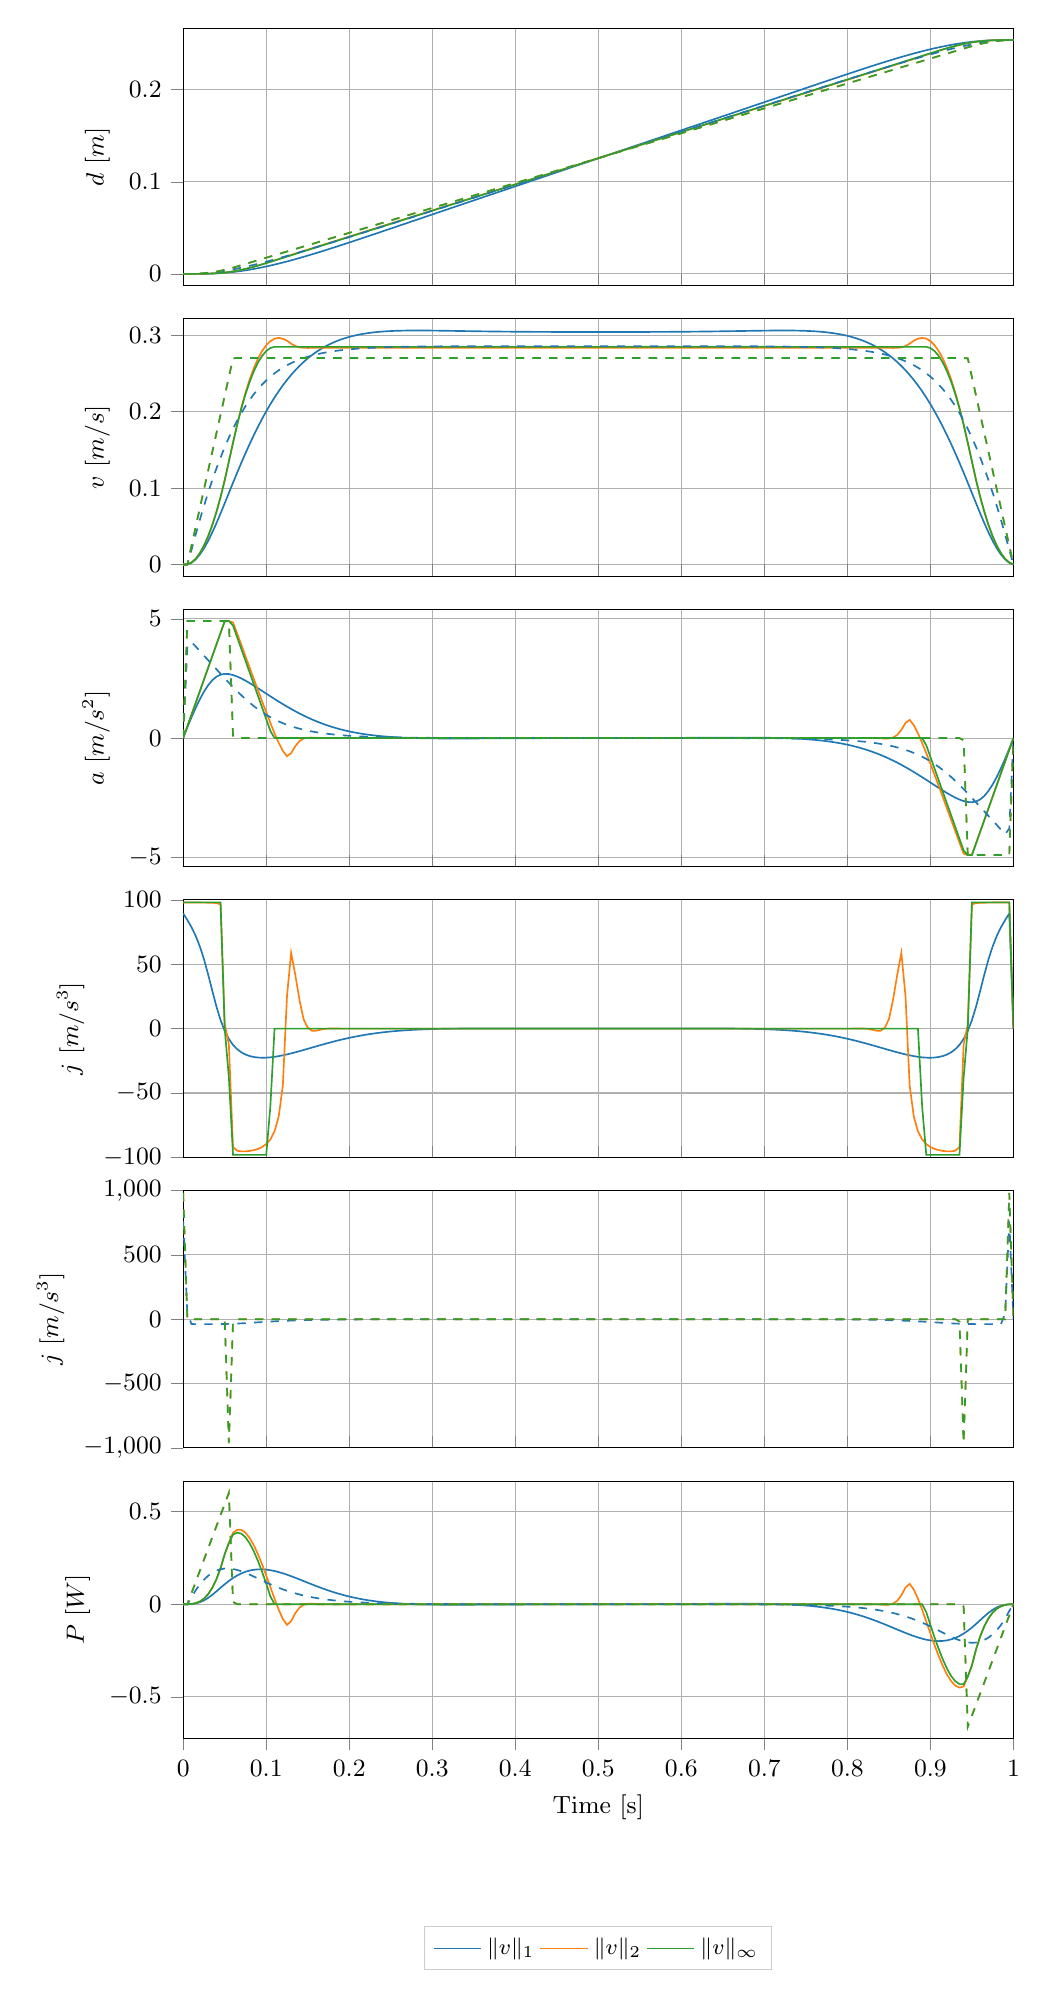
\begin{tikzpicture}

\definecolor{color0}{rgb}{0.12156862745098,0.466666666666667,0.705882352941177}
\definecolor{color1}{rgb}{1,0.498039215686275,0.0549019607843137}
\definecolor{color2}{rgb}{0.172549019607843,0.627450980392157,0.172549019607843}

\begin{groupplot}[group style={group size=1 by 6, vertical sep=12}]
\nextgroupplot[
%legend cell align={left},
%legend entries={{$\|v\|_1$},{$\|v\|_2$},{$\|v\|_\infty$}},
%legend style={at={(0.03,0.97)}, anchor=north west, draw=white!80.0!black},
ytick align=outside,
tick pos=left,
xticklabels={},
x grid style={white!69.01960784313725!black},
xmajorgrids,
xmin=0, xmax=1,
y grid style={white!69.01960784313725!black},
ylabel={$d$ [$m$]},
ymajorgrids,
ymin=-0.0127, ymax=0.2667
%title = \footnotesize{Low $\bar{j}$}
]
%\addlegendimage{no markers, color0}
%\addlegendimage{no markers, color1}
%\addlegendimage{no markers, color2}
\addplot [semithick, color0]
table [row sep=\\]{%
0	0 \\
0.005	0 \\
0.01	4.97841222228891e-59 \\
0.015	1.11882663014615e-05 \\
0.02	4.41115803738754e-05 \\
0.025	0.000108619886324381 \\
0.03	0.000213730411065708 \\
0.035	0.000367436893759766 \\
0.04	0.000576482178960549 \\
0.045	0.000846140945385967 \\
0.05	0.00118009848996838 \\
0.055	0.00158050332644914 \\
0.06	0.00204818096116712 \\
0.065	0.00258291284588478 \\
0.07	0.00318369593859121 \\
0.075	0.00384895072430918 \\
0.08	0.00457667842882801 \\
0.085	0.00536457823051905 \\
0.09	0.00621013531890959 \\
0.095	0.007110688164712 \\
0.1	0.00806348092257906 \\
0.105	0.00906570504014704 \\
0.11	0.0101145328603086 \\
0.115	0.0112071451320338 \\
0.12	0.0123407537579792 \\
0.125	0.0135126207105198 \\
0.13	0.0147200737784828 \\
0.135	0.0159605196232053 \\
0.14	0.0172314544973657 \\
0.145	0.0185304728952884 \\
0.15	0.0198552743469356 \\
0.155	0.0212036685311193 \\
0.16	0.0225735788605822 \\
0.165	0.0239630446781021 \\
0.17	0.0253702221953525 \\
0.175	0.0267933843024235 \\
0.18	0.0282309193738116 \\
0.185	0.0296813291949696 \\
0.19	0.0311432261312617 \\
0.195	0.0326153296578455 \\
0.2	0.034096462364331 \\
0.205	0.0355855455420478 \\
0.21	0.0370815944544977 \\
0.215	0.0385837133833349 \\
0.22	0.0400910905332998 \\
0.225	0.0416029928702529 \\
0.23	0.0431187609570829 \\
0.235	0.0446378038430888 \\
0.24	0.0461595940536333 \\
0.245	0.0476836627186148 \\
0.25	0.0492095948707105 \\
0.255	0.0507370249374636 \\
0.26	0.0522656324451537 \\
0.265	0.0537951379469891 \\
0.27	0.0553252991834896 \\
0.275	0.0568559074789137 \\
0.28	0.0583867843742175 \\
0.285	0.0599177784942126 \\
0.29	0.0614487626443085 \\
0.295	0.062979631130362 \\
0.3	0.0645102972937333 \\
0.305	0.0660406912525294 \\
0.31	0.0675707578392259 \\
0.315	0.0691004547243151 \\
0.32	0.0706297507152973 \\
0.325	0.0721586242201836 \\
0.33	0.0736870618646983 \\
0.335	0.0752150572524753 \\
0.34	0.0767426098577913 \\
0.345	0.0782697240406816 \\
0.35	0.0797964081746598 \\
0.355	0.0813226738776735 \\
0.36	0.0828485353373881 \\
0.365	0.0843740087223643 \\
0.37	0.08589911167119 \\
0.375	0.0874238628521195 \\
0.38	0.0889482815862646 \\
0.385	0.0904723875278768 \\
0.39	0.0919962003957401 \\
0.395	0.0935197397501539 \\
0.4	0.0950430248104321 \\
0.405	0.0965660743082844 \\
0.41	0.0980889063728403 \\
0.415	0.0996115384434745 \\
0.42	0.101133987206955 \\
0.425	0.102656268555779 \\
0.43	0.104178397564882 \\
0.435	0.105700388484204 \\
0.44	0.107222254744862 \\
0.445	0.108744008976971 \\
0.45	0.110265663037326 \\
0.455	0.11178722804544 \\
0.46	0.113308714426578 \\
0.465	0.114830131960628 \\
0.47	0.1163514898358 \\
0.475	0.117872796706283 \\
0.48	0.11939406075313 \\
0.485	0.120915289747716 \\
0.49	0.122436491117253 \\
0.495	0.123957672011884 \\
0.5	0.125478839372977 \\
0.505	0.127000000002263 \\
0.51	0.128521160631525 \\
0.515	0.130042327992544 \\
0.52	0.131563508887053 \\
0.525	0.133084710256421 \\
0.53	0.134605939250791 \\
0.535	0.136127203297376 \\
0.54	0.137648510167552 \\
0.545	0.139169868042371 \\
0.55	0.140691285576029 \\
0.555	0.142212771956738 \\
0.56	0.143734336964389 \\
0.565	0.145255991024253 \\
0.57	0.146777745255849 \\
0.575	0.14829961151598 \\
0.58	0.149821602434761 \\
0.585	0.151343731443317 \\
0.59	0.152866012791586 \\
0.595	0.154388461554506 \\
0.6	0.155911093624576 \\
0.605	0.157433925688566 \\
0.61	0.158956975185853 \\
0.615	0.16048026024557 \\
0.62	0.16200379959943 \\
0.625	0.163527612466751 \\
0.63	0.165051718407837 \\
0.635	0.166576137141478 \\
0.64	0.168100888321932 \\
0.645	0.169625991270316 \\
0.65	0.171151464654892 \\
0.655	0.172677326114254 \\
0.66	0.174203591816967 \\
0.665	0.175730275950702 \\
0.67	0.177257390133411 \\
0.675	0.178784942738611 \\
0.68	0.180312938126342 \\
0.685	0.181841375770882 \\
0.69	0.183370249275867 \\
0.695	0.18489954526702 \\
0.7	0.186429242152351 \\
0.705	0.187959308739357 \\
0.71	0.189489702698529 \\
0.715	0.191020368862341 \\
0.72	0.192551237348893 \\
0.725	0.194082221499541 \\
0.73	0.195613215620135 \\
0.735	0.197144092516073 \\
0.74	0.198674700812159 \\
0.745	0.200204862049338 \\
0.75	0.201734367551862 \\
0.755	0.203262975060242 \\
0.76	0.204790405127679 \\
0.765	0.206316337280442 \\
0.77	0.207840405946064 \\
0.775	0.209362196157209 \\
0.78	0.210881239043763 \\
0.785	0.212397007131081 \\
0.79	0.213908909468456 \\
0.795	0.215416286618771 \\
0.8	0.216918405547883 \\
0.805	0.218414454460528 \\
0.81	0.21990353763836 \\
0.815	0.22138467034488 \\
0.82	0.222856773871421 \\
0.825	0.224318670807599 \\
0.83	0.225769080628581 \\
0.835	0.227206615699742 \\
0.84	0.228629777806548 \\
0.845	0.230036955323507 \\
0.85	0.231426421140722 \\
0.855	0.232796331469878 \\
0.86	0.234144725653765 \\
0.865	0.235469527105135 \\
0.87	0.236768545502807 \\
0.875	0.238039480376752 \\
0.88	0.239279926221298 \\
0.885	0.240487379289122 \\
0.89	0.241659246241563 \\
0.895	0.242792854867444 \\
0.9	0.243885467139138 \\
0.905	0.244934294959297 \\
0.91	0.24593651907689 \\
0.915	0.246889311834804 \\
0.92	0.247789864680671 \\
0.925	0.248635421769139 \\
0.93	0.249423321570914 \\
0.935	0.250151049275515 \\
0.94	0.250816304061309 \\
0.945	0.251417087154078 \\
0.95	0.251951819038842 \\
0.955	0.252419496673588 \\
0.96	0.252819901510079 \\
0.965	0.253153859054658 \\
0.97	0.253423517821073 \\
0.975	0.253632563106261 \\
0.98	0.253786269588945 \\
0.985	0.25389138011368 \\
0.99	0.253955888419628 \\
0.995	0.253988811733699 \\
1	0.254 \\
};
\addplot [semithick, color1]
table [row sep=\\]{%
0	0 \\
0.005	1.06658667518364e-41 \\
0.01	-1.18561116295309e-41 \\
0.015	1.22564937587801e-05 \\
0.02	4.90239363036012e-05 \\
0.025	0.000122554365077358 \\
0.03	0.000245096735395254 \\
0.035	0.000428895979626159 \\
0.04	0.000686191699208123 \\
0.045	0.00102921616555437 \\
0.05	0.00147019031515712 \\
0.055	0.00202131133163284 \\
0.06	0.00269464437145003 \\
0.065	0.00349060240651143 \\
0.07	0.00440764064118935 \\
0.075	0.0054342539515717 \\
0.08	0.00655858532427453 \\
0.085	0.0077687117019199 \\
0.09	0.00905271285991824 \\
0.095	0.0103987089122039 \\
0.1	0.0117948951563319 \\
0.105	0.0132295859484796 \\
0.11	0.014691278943485 \\
0.115	0.0161687575596495 \\
0.12	0.0176512657423345 \\
0.125	0.0191288281870075 \\
0.13	0.0205928986940453 \\
0.135	0.0220379475667957 \\
0.14	0.0234671266587109 \\
0.145	0.0248878059844904 \\
0.15	0.0263052032098831 \\
0.155	0.0277221143567249 \\
0.16	0.0291394503599918 \\
0.165	0.0305572987352749 \\
0.17	0.0319754594581752 \\
0.175	0.0333937310965911 \\
0.18	0.0348120083795423 \\
0.185	0.0362302639284566 \\
0.19	0.037648505241612 \\
0.195	0.0390667465384287 \\
0.2	0.0404849976015637 \\
0.205	0.0419032620211205 \\
0.21	0.0433215389435684 \\
0.215	0.0447398253797589 \\
0.22	0.0461581179401846 \\
0.225	0.0475764137657653 \\
0.23	0.0489947108170905 \\
0.235	0.0504130077960133 \\
0.24	0.0518313039342342 \\
0.245	0.0532495987903341 \\
0.25	0.0546678921102522 \\
0.255	0.0560861837517568 \\
0.26	0.0575044736512391 \\
0.265	0.058922761810007 \\
0.27	0.0603410482850696 \\
0.275	0.061759333177993 \\
0.28	0.063177616621212 \\
0.285	0.0645958987637245 \\
0.29	0.0660141797583744 \\
0.295	0.0674324597521378 \\
0.3	0.0688507388798371 \\
0.305	0.0702690172609657 \\
0.31	0.0716872949989143 \\
0.315	0.0731055721818005 \\
0.32	0.0745238488841911 \\
0.325	0.0759421251691788 \\
0.33	0.077360401090454 \\
0.335	0.0787786766941634 \\
0.34	0.0801969520204627 \\
0.345	0.0816152271047447 \\
0.35	0.0830335019785666 \\
0.355	0.0844517766703255 \\
0.36	0.085870051205734 \\
0.365	0.087288325608149 \\
0.37	0.0887065998987958 \\
0.375	0.0901248740969252 \\
0.38	0.0915431482199297 \\
0.385	0.0929614222834372 \\
0.39	0.0943796963013946 \\
0.395	0.0957979702861503 \\
0.4	0.097216244248537 \\
0.405	0.0986345181979588 \\
0.41	0.10005279214248 \\
0.415	0.101471066088916 \\
0.42	0.102889340042927 \\
0.425	0.104307614009109 \\
0.43	0.105725887991082 \\
0.435	0.107144161991579 \\
0.44	0.10856243601253 \\
0.445	0.10998071005514 \\
0.45	0.111398984119964 \\
0.455	0.112817258206981 \\
0.46	0.114235532315655 \\
0.465	0.115653806445005 \\
0.47	0.117072080593652 \\
0.475	0.118490354759883 \\
0.48	0.119908628941696 \\
0.485	0.121326903136848 \\
0.49	0.1227451773429 \\
0.495	0.12416345155726 \\
0.5	0.12558172577722 \\
0.505	0.127 \\
0.51	0.12841827422278 \\
0.515	0.12983654844274 \\
0.52	0.1312548226571 \\
0.525	0.132673096863152 \\
0.53	0.134091371058304 \\
0.535	0.135509645240117 \\
0.54	0.136927919406348 \\
0.545	0.138346193554995 \\
0.55	0.139764467684345 \\
0.555	0.141182741793019 \\
0.56	0.142601015880036 \\
0.565	0.14401928994486 \\
0.57	0.14543756398747 \\
0.575	0.146855838008421 \\
0.58	0.148274112008918 \\
0.585	0.149692385990891 \\
0.59	0.151110659957073 \\
0.595	0.152528933911084 \\
0.6	0.15394720785752 \\
0.605	0.155365481802041 \\
0.61	0.156783755751463 \\
0.615	0.15820202971385 \\
0.62	0.159620303698605 \\
0.625	0.161038577716563 \\
0.63	0.16245685178007 \\
0.635	0.163875125903075 \\
0.64	0.165293400101204 \\
0.645	0.166711674391851 \\
0.65	0.168129948794266 \\
0.655	0.169548223329675 \\
0.66	0.170966498021433 \\
0.665	0.172384772895255 \\
0.67	0.173803047979537 \\
0.675	0.175221323305837 \\
0.68	0.176639598909546 \\
0.685	0.178057874830821 \\
0.69	0.179476151115809 \\
0.695	0.1808944278182 \\
0.7	0.182312705001086 \\
0.705	0.183730982739034 \\
0.71	0.185149261120163 \\
0.715	0.186567540247862 \\
0.72	0.187985820241626 \\
0.725	0.189404101236276 \\
0.73	0.190822383378788 \\
0.735	0.192240666822007 \\
0.74	0.19365895171493 \\
0.745	0.195077238189993 \\
0.75	0.196495526348761 \\
0.755	0.197913816248243 \\
0.76	0.199332107889748 \\
0.765	0.200750401209666 \\
0.77	0.202168696065766 \\
0.775	0.203586992203987 \\
0.78	0.205005289182909 \\
0.785	0.206423586234235 \\
0.79	0.207841882059815 \\
0.795	0.209260174620241 \\
0.8	0.210678461056432 \\
0.805	0.212096737978879 \\
0.81	0.213515002398436 \\
0.815	0.214933253461571 \\
0.82	0.216351494758388 \\
0.825	0.217769736071543 \\
0.83	0.219187991620458 \\
0.835	0.220606268903409 \\
0.84	0.222024540541825 \\
0.845	0.223442701264725 \\
0.85	0.224860549640008 \\
0.855	0.226277885643275 \\
0.86	0.227694796790117 \\
0.865	0.22911219401551 \\
0.87	0.230532873341289 \\
0.875	0.231962052433204 \\
0.88	0.233407101305955 \\
0.885	0.234871171812993 \\
0.89	0.236348734257666 \\
0.895	0.23783124244035 \\
0.9	0.239308721056515 \\
0.905	0.24077041405152 \\
0.91	0.242205104843668 \\
0.915	0.243601291087796 \\
0.92	0.244947287140082 \\
0.925	0.24623128829808 \\
0.93	0.247441414675725 \\
0.935	0.248565746048428 \\
0.94	0.249592359358811 \\
0.945	0.250509397593489 \\
0.95	0.25130535562855 \\
0.955	0.251978688668367 \\
0.96	0.252529809684843 \\
0.965	0.252970783834446 \\
0.97	0.253313808300792 \\
0.975	0.253571104020374 \\
0.98	0.253754903264605 \\
0.985	0.253877445634923 \\
0.99	0.253950976063696 \\
0.995	0.253987743506241 \\
1	0.254 \\
};
\addplot [semithick, color2]
table [row sep=\\]{%
0	0 \\
0.005	4.01047944496259e-36 \\
0.01	-5.85679849578213e-23 \\
0.015	1.22624929974272e-05 \\
0.02	4.90499707916886e-05 \\
0.025	0.000122624923647846 \\
0.03	0.000245249839788283 \\
0.035	0.000429187204597117 \\
0.04	0.00068669949929599 \\
0.045	0.00103004919852011 \\
0.05	0.0014714987651112 \\
0.055	0.00202331063547746 \\
0.06	0.00269774713807133 \\
0.065	0.0034948085026472 \\
0.07	0.0044097479719172 \\
0.075	0.00543030321535724 \\
0.08	0.00654421182814049 \\
0.085	0.0077392113827782 \\
0.09	0.0090030394427219 \\
0.095	0.0103234335688859 \\
0.1	0.0116881313247409 \\
0.105	0.013084870282945 \\
0.11	0.0145013880392891 \\
0.115	0.0159254222621307 \\
0.12	0.0173494551967736 \\
0.125	0.0187734881427431 \\
0.13	0.0201975215811617 \\
0.135	0.0216215545155533 \\
0.14	0.0230455876424411 \\
0.145	0.0244696206783009 \\
0.15	0.0258936537032167 \\
0.155	0.0273176867405598 \\
0.16	0.0287417197887991 \\
0.165	0.0301657528448728 \\
0.17	0.0315897859034955 \\
0.175	0.0330138189611305 \\
0.18	0.034437852016469 \\
0.185	0.0358618850695266 \\
0.19	0.037285918120836 \\
0.195	0.0387099511709705 \\
0.2	0.0401339842203534 \\
0.205	0.0415580172692342 \\
0.21	0.0429820503177316 \\
0.215	0.0444060833658894 \\
0.22	0.0458301164137186 \\
0.225	0.0472541494612241 \\
0.23	0.0486781825084164 \\
0.235	0.0501022155553154 \\
0.24	0.0515262486019489 \\
0.245	0.0529502816483507 \\
0.25	0.0543743146945579 \\
0.255	0.055798347740608 \\
0.26	0.0572223807865382 \\
0.265	0.0586464138323832 \\
0.27	0.0600704468781753 \\
0.275	0.0614944799239435 \\
0.28	0.0629185129697133 \\
0.285	0.0643425460155076 \\
0.29	0.0657665790613463 \\
0.295	0.0671906121072473 \\
0.3	0.0686146451532256 \\
0.305	0.0700386781992927 \\
0.31	0.0714627112454541 \\
0.315	0.0728867442917069 \\
0.32	0.0743107773380363 \\
0.325	0.0757348103844144 \\
0.33	0.0771588434308029 \\
0.335	0.0785828764771611 \\
0.34	0.0800069095234592 \\
0.345	0.0814309425696926 \\
0.35	0.0828549756158876 \\
0.355	0.0842790086620837 \\
0.36	0.0857030417082793 \\
0.365	0.0871270747543502 \\
0.37	0.088551107800016 \\
0.375	0.0899751408449521 \\
0.38	0.0913991738890307 \\
0.385	0.0928232069325504 \\
0.39	0.0942472399762824 \\
0.395	0.0956712730210666 \\
0.4	0.0970953060670962 \\
0.405	0.0985193391137935 \\
0.41	0.0999433721604925 \\
0.415	0.101367405206979 \\
0.42	0.102791438253412 \\
0.425	0.104215471299994 \\
0.43	0.105639504346763 \\
0.435	0.107063537393559 \\
0.44	0.108487570440113 \\
0.445	0.109911603486146 \\
0.45	0.11133563653144 \\
0.455	0.112759669575882 \\
0.46	0.114183702619485 \\
0.465	0.115607735662389 \\
0.47	0.11703176870484 \\
0.475	0.118455801747153 \\
0.48	0.119879834789637 \\
0.485	0.121303867832395 \\
0.49	0.122727900875119 \\
0.495	0.124151933917302 \\
0.5	0.125575966958821 \\
0.505	0.127 \\
0.51	0.128424033041179 \\
0.515	0.129848066082698 \\
0.52	0.131272099124881 \\
0.525	0.132696132167605 \\
0.53	0.134120165210363 \\
0.535	0.135544198252846 \\
0.54	0.13696823129516 \\
0.545	0.138392264337611 \\
0.55	0.139816297380515 \\
0.555	0.141240330424118 \\
0.56	0.14266436346856 \\
0.565	0.144088396513854 \\
0.57	0.145512429559887 \\
0.575	0.146936462606441 \\
0.58	0.148360495653237 \\
0.585	0.149784528700006 \\
0.59	0.151208561746588 \\
0.595	0.152632594793021 \\
0.6	0.154056627839507 \\
0.605	0.155480660886206 \\
0.61	0.156904693932904 \\
0.615	0.158328726978933 \\
0.62	0.159752760023718 \\
0.625	0.16117679306745 \\
0.63	0.162600826110969 \\
0.635	0.164024859155048 \\
0.64	0.165448892199984 \\
0.645	0.16687292524565 \\
0.65	0.168296958291721 \\
0.655	0.169720991337916 \\
0.66	0.171145024384112 \\
0.665	0.172569057430307 \\
0.67	0.173993090476541 \\
0.675	0.175417123522839 \\
0.68	0.176841156569197 \\
0.685	0.178265189615586 \\
0.69	0.179689222661964 \\
0.695	0.181113255708293 \\
0.7	0.182537288754546 \\
0.705	0.183961321800707 \\
0.71	0.185385354846774 \\
0.715	0.186809387892753 \\
0.72	0.188233420938654 \\
0.725	0.189657453984492 \\
0.73	0.191081487030287 \\
0.735	0.192505520076057 \\
0.74	0.193929553121825 \\
0.745	0.195353586167617 \\
0.75	0.196777619213462 \\
0.755	0.198201652259392 \\
0.76	0.199625685305442 \\
0.765	0.201049718351649 \\
0.77	0.202473751398051 \\
0.775	0.203897784444685 \\
0.78	0.205321817491584 \\
0.785	0.206745850538776 \\
0.79	0.208169883586281 \\
0.795	0.209593916634111 \\
0.8	0.211017949682268 \\
0.805	0.212441982730766 \\
0.81	0.213866015779647 \\
0.815	0.215290048829029 \\
0.82	0.216714081879164 \\
0.825	0.218138114930473 \\
0.83	0.219562147983531 \\
0.835	0.220986181038869 \\
0.84	0.222410214096504 \\
0.845	0.223834247155127 \\
0.85	0.225258280211201 \\
0.855	0.22668231325944 \\
0.86	0.228106346296783 \\
0.865	0.229530379321699 \\
0.87	0.230954412357559 \\
0.875	0.232378445484447 \\
0.88	0.233802478418838 \\
0.885	0.235226511857257 \\
0.89	0.236650544803226 \\
0.895	0.238074577737869 \\
0.9	0.239498611960711 \\
0.905	0.240915129717055 \\
0.91	0.242311868675259 \\
0.915	0.243676566431114 \\
0.92	0.244996960557278 \\
0.925	0.246260788617222 \\
0.93	0.24745578817186 \\
0.935	0.248569696784643 \\
0.94	0.249590252028083 \\
0.945	0.250505191497353 \\
0.95	0.251302252861929 \\
0.955	0.251976689364523 \\
0.96	0.252528501234889 \\
0.965	0.25296995080148 \\
0.97	0.253313300500704 \\
0.975	0.253570812795403 \\
0.98	0.253754750160212 \\
0.985	0.253877375076352 \\
0.99	0.253950950029208 \\
0.995	0.253987737507003 \\
1	0.254 \\
};
\addplot [semithick, color0,dashed]
table [row sep=\\]{%
0	0 \\
0.005	3.1861838222649e-58 \\
0.01	0 \\
0.015	9.50261228537274e-05 \\
0.02	0.000290690697085654 \\
0.025	0.00058237586316443 \\
0.03	0.000965234240263295 \\
0.035	0.00143449718218089 \\
0.04	0.00198542186576523 \\
0.045	0.002613261170158 \\
0.05	0.00331326043160454 \\
0.055	0.00408067211366791 \\
0.06	0.00491078223036921 \\
0.065	0.00579894399153219 \\
0.07	0.00674061486707412 \\
0.075	0.0077313937328332 \\
0.08	0.00876705527181334 \\
0.085	0.00984357944736526 \\
0.09	0.0109571746080189 \\
0.095	0.0121042935409427 \\
0.1	0.0132816424713788 \\
0.105	0.0144861835410961 \\
0.11	0.0157151316587486 \\
0.115	0.0169659468013914 \\
0.12	0.018236322886913 \\
0.125	0.0195241742713767 \\
0.13	0.0208276207938643 \\
0.135	0.0221449721291344 \\
0.14	0.0234747120421442 \\
0.145	0.0248154829840203 \\
0.15	0.0261660713363183 \\
0.155	0.0275253935014464 \\
0.16	0.0288924829532324 \\
0.165	0.0302664782980572 \\
0.17	0.0316466123511006 \\
0.175	0.0330322022019987 \\
0.18	0.0344226402231088 \\
0.185	0.0358173859616631 \\
0.19	0.0372159588512115 \\
0.195	0.0386179316747721 \\
0.2	0.040022924714 \\
0.205	0.0414306005199482 \\
0.21	0.0428406592451059 \\
0.215	0.0442528344805749 \\
0.22	0.045666889546874 \\
0.225	0.0470826141907253 \\
0.23	0.0484998216449236 \\
0.235	0.0499183460125454 \\
0.24	0.0513380399405073 \\
0.245	0.0527587725508657 \\
0.25	0.0541804276017836 \\
0.255	0.0556029018531695 \\
0.26	0.057026103614101 \\
0.265	0.0584499514521539 \\
0.27	0.0598743730465412 \\
0.275	0.0612993041692569 \\
0.28	0.0627246877800189 \\
0.285	0.064150473222181 \\
0.29	0.0655766155086503 \\
0.295	0.0670030746875405 \\
0.3	0.0684298152787981 \\
0.305	0.0698568057736644 \\
0.31	0.0712840181902129 \\
0.315	0.072711427678587 \\
0.32	0.0741390121702958 \\
0.325	0.075566752066832 \\
0.33	0.0769946299631587 \\
0.335	0.0784226304021767 \\
0.34	0.0798507396565012 \\
0.345	0.0812789455347929 \\
0.35	0.0827072372095691 \\
0.355	0.0841356050643837 \\
0.36	0.0855640405581276 \\
0.365	0.0869925361045324 \\
0.37	0.0884210849651191 \\
0.375	0.0898496811540506 \\
0.38	0.0912783193536308 \\
0.385	0.0927069948392167 \\
0.39	0.0941357034125366 \\
0.395	0.0955644413424629 \\
0.4	0.096993205312243 \\
0.405	0.0984219923727577 \\
0.41	0.0998507999007956 \\
0.415	0.101279625562141 \\
0.42	0.102708467278584 \\
0.425	0.104137323198581 \\
0.43	0.105566191671051 \\
0.435	0.106995071222108 \\
0.44	0.108423960534316 \\
0.445	0.109852858427953 \\
0.45	0.111281763844492 \\
0.455	0.11271067583166 \\
0.46	0.11413959352995 \\
0.465	0.11556851616043 \\
0.47	0.116997443013745 \\
0.475	0.118426373440197 \\
0.48	0.119855306840616 \\
0.485	0.1212842426578 \\
0.49	0.122713180368654 \\
0.495	0.124142119476835 \\
0.5	0.125571059505744 \\
0.505	0.126999999991766 \\
0.51	0.12842894047779 \\
0.515	0.129857880506721 \\
0.52	0.131286819614971 \\
0.525	0.132715757325938 \\
0.53	0.134144693143297 \\
0.535	0.135573626543943 \\
0.54	0.137002556970614 \\
0.545	0.138431483824078 \\
0.55	0.139860406454658 \\
0.555	0.141289324153006 \\
0.56	0.142718236140214 \\
0.565	0.144147141556785 \\
0.57	0.145576039450417 \\
0.575	0.147004928762629 \\
0.58	0.148433808313746 \\
0.585	0.149862676786313 \\
0.59	0.151291532706424 \\
0.595	0.152720374422995 \\
0.6	0.154149200084487 \\
0.605	0.155578007612673 \\
0.61	0.157006794673359 \\
0.615	0.158435558643303 \\
0.62	0.159864296573378 \\
0.625	0.161293005146778 \\
0.63	0.162721680632276 \\
0.635	0.164150318831625 \\
0.64	0.165578915020207 \\
0.645	0.167007463880294 \\
0.65	0.168435959425996 \\
0.655	0.169864394918867 \\
0.66	0.171292762772652 \\
0.665	0.172721054446225 \\
0.67	0.174149260323202 \\
0.675	0.175577369576105 \\
0.68	0.177005370013618 \\
0.685	0.178433247908379 \\
0.69	0.17986098780334 \\
0.695	0.181288572293598 \\
0.7	0.182715981780711 \\
0.705	0.184143194196205 \\
0.71	0.185570184690227 \\
0.715	0.18699692528081 \\
0.72	0.188423384459159 \\
0.725	0.189849526745192 \\
0.73	0.191275312187078 \\
0.735	0.192700695797785 \\
0.74	0.194125626920698 \\
0.745	0.195550048515525 \\
0.75	0.196973896354255 \\
0.755	0.198397098116064 \\
0.76	0.199819572368457 \\
0.765	0.201241227420497 \\
0.77	0.20266196003203 \\
0.775	0.204081653961194 \\
0.78	0.205500178329993 \\
0.785	0.206917385785313 \\
0.79	0.208333110430252 \\
0.795	0.209747165497609 \\
0.8	0.211159340734057 \\
0.805	0.212569399460041 \\
0.81	0.213977075266575 \\
0.815	0.215382068306079 \\
0.82	0.216784041129655 \\
0.825	0.21818261401906 \\
0.83	0.219577359757471 \\
0.835	0.220967797778437 \\
0.84	0.222353387629224 \\
0.845	0.223733521682145 \\
0.85	0.225107517026764 \\
0.855	0.226474606478222 \\
0.86	0.227833928642997 \\
0.865	0.22918451699505 \\
0.87	0.23052528793686 \\
0.875	0.231855027850016 \\
0.88	0.233172379185819 \\
0.885	0.234475825709236 \\
0.89	0.235763677094945 \\
0.895	0.237034053181949 \\
0.9	0.238284868326322 \\
0.905	0.239513816445905 \\
0.91	0.24071835751767 \\
0.915	0.241895706450058 \\
0.92	0.243042825384793 \\
0.925	0.244156420547159 \\
0.93	0.245232944724325 \\
0.935	0.246268606264749 \\
0.94	0.247259385131645 \\
0.945	0.248201056007969 \\
0.95	0.249089217769601 \\
0.955	0.249919327886544 \\
0.96	0.250686739568713 \\
0.965	0.251386738830172 \\
0.97	0.252014578134509 \\
0.975	0.252565502818007 \\
0.98	0.253034765759856 \\
0.985	0.253417624136907 \\
0.99	0.253709309302945 \\
0.995	0.253904973877155 \\
1	0.254 \\
};
\addplot [semithick, color1,dashed]
table [row sep=\\]{%
0	0 \\
0.005	3.50735115154921e-53 \\
0.01	-9.08322381945395e-52 \\
0.015	0.000122624996642986 \\
0.02	0.000367874991235329 \\
0.025	0.000735749983265719 \\
0.03	0.0012262499720044 \\
0.035	0.00183937495635808 \\
0.04	0.00257512493458052 \\
0.045	0.00343349990362343 \\
0.05	0.00441449985741509 \\
0.055	0.0055181247808942 \\
0.06	0.00674437461510253 \\
0.065	0.00809324523871019 \\
0.07	0.0094444697227753 \\
0.075	0.0107956827180545 \\
0.08	0.0121468957096879 \\
0.085	0.0134981087013386 \\
0.09	0.0148493216929893 \\
0.095	0.0162005346846401 \\
0.1	0.0175517476762908 \\
0.105	0.0189029606679415 \\
0.11	0.0202541736595922 \\
0.115	0.021605386651243 \\
0.12	0.0229565996428937 \\
0.125	0.0243078126345444 \\
0.13	0.0256590256261952 \\
0.135	0.0270102386178459 \\
0.14	0.0283614516094966 \\
0.145	0.0297126646011474 \\
0.15	0.0310638775927981 \\
0.155	0.0324150905844488 \\
0.16	0.0337663035760996 \\
0.165	0.0351175165677503 \\
0.17	0.036468729559401 \\
0.175	0.0378199425510517 \\
0.18	0.0391711555427025 \\
0.185	0.0405223685343532 \\
0.19	0.0418735815260039 \\
0.195	0.0432247945176547 \\
0.2	0.0445760075093054 \\
0.205	0.0459272205009561 \\
0.21	0.0472784334926069 \\
0.215	0.0486296464842576 \\
0.22	0.0499808594759083 \\
0.225	0.0513320724675591 \\
0.23	0.0526832854592098 \\
0.235	0.0540344984508605 \\
0.24	0.0553857114425112 \\
0.245	0.056736924434162 \\
0.25	0.0580881374258127 \\
0.255	0.0594393504174634 \\
0.26	0.0607905634091142 \\
0.265	0.0621417764007649 \\
0.27	0.0634929893924156 \\
0.275	0.0648442023840664 \\
0.28	0.0661954153757171 \\
0.285	0.0675466283673678 \\
0.29	0.0688978413590186 \\
0.295	0.0702490543506693 \\
0.3	0.07160026734232 \\
0.305	0.0729514803339708 \\
0.31	0.0743026933256215 \\
0.315	0.0756539063172722 \\
0.32	0.0770051193089229 \\
0.325	0.0783563323005737 \\
0.33	0.0797075452922244 \\
0.335	0.0810587582838751 \\
0.34	0.0824099712755259 \\
0.345	0.0837611842671766 \\
0.35	0.0851123972588273 \\
0.355	0.0864636102504781 \\
0.36	0.0878148232421288 \\
0.365	0.0891660362337795 \\
0.37	0.0905172492254303 \\
0.375	0.091868462217081 \\
0.38	0.0932196752087317 \\
0.385	0.0945708882003825 \\
0.39	0.0959221011920332 \\
0.395	0.0972733141836839 \\
0.4	0.0986245271753346 \\
0.405	0.0999757401669854 \\
0.41	0.101326953158636 \\
0.415	0.102678166150287 \\
0.42	0.104029379141938 \\
0.425	0.105380592133588 \\
0.43	0.106731805125239 \\
0.435	0.10808301811689 \\
0.44	0.10943423110854 \\
0.445	0.110785444100191 \\
0.45	0.112136657091842 \\
0.455	0.113487870083493 \\
0.46	0.114839083075143 \\
0.465	0.116190296066794 \\
0.47	0.117541509058445 \\
0.475	0.118892722050096 \\
0.48	0.120243935041746 \\
0.485	0.121595148033397 \\
0.49	0.122946361025048 \\
0.495	0.124297574016699 \\
0.5	0.125648787008349 \\
0.505	0.127 \\
0.51	0.128351212991651 \\
0.515	0.129702425983301 \\
0.52	0.131053638974952 \\
0.525	0.132404851966603 \\
0.53	0.133756064958254 \\
0.535	0.135107277949904 \\
0.54	0.136458490941555 \\
0.545	0.137809703933206 \\
0.55	0.139160916924857 \\
0.555	0.140512129916507 \\
0.56	0.141863342908158 \\
0.565	0.143214555899809 \\
0.57	0.14456576889146 \\
0.575	0.14591698188311 \\
0.58	0.147268194874761 \\
0.585	0.148619407866412 \\
0.59	0.149970620858062 \\
0.595	0.151321833849713 \\
0.6	0.152673046841364 \\
0.605	0.154024259833015 \\
0.61	0.155375472824665 \\
0.615	0.156726685816316 \\
0.62	0.158077898807967 \\
0.625	0.159429111799618 \\
0.63	0.160780324791268 \\
0.635	0.162131537782919 \\
0.64	0.16348275077457 \\
0.645	0.16483396376622 \\
0.65	0.166185176757871 \\
0.655	0.167536389749522 \\
0.66	0.168887602741173 \\
0.665	0.170238815732823 \\
0.67	0.171590028724474 \\
0.675	0.172941241716125 \\
0.68	0.174292454707776 \\
0.685	0.175643667699426 \\
0.69	0.176994880691077 \\
0.695	0.178346093682728 \\
0.7	0.179697306674378 \\
0.705	0.181048519666029 \\
0.71	0.18239973265768 \\
0.715	0.183750945649331 \\
0.72	0.185102158640981 \\
0.725	0.186453371632632 \\
0.73	0.187804584624283 \\
0.735	0.189155797615934 \\
0.74	0.190507010607584 \\
0.745	0.191858223599235 \\
0.75	0.193209436590886 \\
0.755	0.194560649582537 \\
0.76	0.195911862574187 \\
0.765	0.197263075565838 \\
0.77	0.198614288557489 \\
0.775	0.199965501549139 \\
0.78	0.20131671454079 \\
0.785	0.202667927532441 \\
0.79	0.204019140524092 \\
0.795	0.205370353515742 \\
0.8	0.206721566507393 \\
0.805	0.208072779499044 \\
0.81	0.209423992490695 \\
0.815	0.210775205482345 \\
0.82	0.212126418473996 \\
0.825	0.213477631465647 \\
0.83	0.214828844457297 \\
0.835	0.216180057448948 \\
0.84	0.217531270440599 \\
0.845	0.21888248343225 \\
0.85	0.2202336964239 \\
0.855	0.221584909415551 \\
0.86	0.222936122407202 \\
0.865	0.224287335398853 \\
0.87	0.225638548390503 \\
0.875	0.226989761382154 \\
0.88	0.228340974373805 \\
0.885	0.229692187365456 \\
0.89	0.231043400357106 \\
0.895	0.232394613348757 \\
0.9	0.233745826340408 \\
0.905	0.235097039332058 \\
0.91	0.236448252323709 \\
0.915	0.23779946531536 \\
0.92	0.239150678307011 \\
0.925	0.240501891298661 \\
0.93	0.241853104290312 \\
0.935	0.243204317281945 \\
0.94	0.244555530277225 \\
0.945	0.24590675476129 \\
0.95	0.247255625384897 \\
0.955	0.248481875219106 \\
0.96	0.249585500142585 \\
0.965	0.250566500096377 \\
0.97	0.251424875065419 \\
0.975	0.252160625043642 \\
0.98	0.252773750027996 \\
0.985	0.253264250016734 \\
0.99	0.253632125008765 \\
0.995	0.253877375003357 \\
1	0.254 \\
};
\addplot [semithick, color2,dashed]
table [row sep=\\]{%
0	0 \\
0.005	9.38936663520068e-50 \\
0.01	-2.29588740394978e-41 \\
0.015	0.000122624854529997 \\
0.02	0.000367874629050668 \\
0.025	0.000735749314671039 \\
0.03	0.00122624890027711 \\
0.035	0.00183937337157899 \\
0.04	0.00257512270952269 \\
0.045	0.00343349688743103 \\
0.05	0.00441449586528488 \\
0.055	0.00551811957637658 \\
0.06	0.00674436788725691 \\
0.065	0.00809324039705354 \\
0.07	0.00944445357487962 \\
0.075	0.0107956667521677 \\
0.08	0.0121468799294554 \\
0.085	0.0134980931067431 \\
0.09	0.0148493062840308 \\
0.095	0.0162005194613185 \\
0.1	0.0175517326386062 \\
0.105	0.0189029458158938 \\
0.11	0.0202541589931815 \\
0.115	0.0216053721704692 \\
0.12	0.0229565853477569 \\
0.125	0.0243077985250446 \\
0.13	0.0256590117023323 \\
0.135	0.02701022487962 \\
0.14	0.0283614380569076 \\
0.145	0.0297126512341953 \\
0.15	0.031063864411483 \\
0.155	0.0324150775887707 \\
0.16	0.0337662907660584 \\
0.165	0.0351175039433461 \\
0.17	0.0364687171206338 \\
0.175	0.0378199302979214 \\
0.18	0.0391711434752091 \\
0.185	0.0405223566524968 \\
0.19	0.0418735698297845 \\
0.195	0.0432247830070722 \\
0.2	0.0445759961843599 \\
0.205	0.0459272093616475 \\
0.21	0.0472784225389352 \\
0.215	0.0486296357162229 \\
0.22	0.0499808488935106 \\
0.225	0.0513320620707983 \\
0.23	0.052683275248086 \\
0.235	0.0540344884253736 \\
0.24	0.0553857016026613 \\
0.245	0.056736914779949 \\
0.25	0.0580881279572367 \\
0.255	0.0594393411345244 \\
0.26	0.0607905543118121 \\
0.265	0.0621417674890997 \\
0.27	0.0634929806663874 \\
0.275	0.0648441938436751 \\
0.28	0.0661954070209628 \\
0.285	0.0675466201982505 \\
0.29	0.0688978333755382 \\
0.295	0.0702490465528259 \\
0.3	0.0716002597301135 \\
0.305	0.0729514729074012 \\
0.31	0.0743026860846889 \\
0.315	0.0756538992619766 \\
0.32	0.0770051124392643 \\
0.325	0.078356325616552 \\
0.33	0.0797075387938396 \\
0.335	0.0810587519711273 \\
0.34	0.082409965148415 \\
0.345	0.0837611783257027 \\
0.35	0.0851123915029904 \\
0.355	0.0864636046802781 \\
0.36	0.0878148178575657 \\
0.365	0.0891660310348534 \\
0.37	0.0905172442121411 \\
0.375	0.0918684573894288 \\
0.38	0.0932196705667165 \\
0.385	0.0945708837440042 \\
0.39	0.0959220969212918 \\
0.395	0.0972733100985795 \\
0.4	0.0986245232758672 \\
0.405	0.0999757364531549 \\
0.41	0.101326949630443 \\
0.415	0.10267816280773 \\
0.42	0.104029375985018 \\
0.425	0.105380589162306 \\
0.43	0.106731802339593 \\
0.435	0.108083015516881 \\
0.44	0.109434228694169 \\
0.445	0.110785441871456 \\
0.45	0.112136655048744 \\
0.455	0.113487868226032 \\
0.46	0.114839081403319 \\
0.465	0.116190294580607 \\
0.47	0.117541507757895 \\
0.475	0.118892720935182 \\
0.48	0.12024393411247 \\
0.485	0.121595147289758 \\
0.49	0.122946360467046 \\
0.495	0.124297573644333 \\
0.5	0.125648786821621 \\
0.505	0.126999999998909 \\
0.51	0.128351213176196 \\
0.515	0.129702426353484 \\
0.52	0.131053639530772 \\
0.525	0.132404852708059 \\
0.53	0.133756065885347 \\
0.535	0.135107279062635 \\
0.54	0.136458492239922 \\
0.545	0.13780970541721 \\
0.55	0.139160918594498 \\
0.555	0.140512131771785 \\
0.56	0.141863344949073 \\
0.565	0.143214558126361 \\
0.57	0.144565771303648 \\
0.575	0.145916984480936 \\
0.58	0.147268197658224 \\
0.585	0.148619410835512 \\
0.59	0.149970624012799 \\
0.595	0.151321837190087 \\
0.6	0.152673050367375 \\
0.605	0.154024263544662 \\
0.61	0.15537547672195 \\
0.615	0.156726689899238 \\
0.62	0.158077903076525 \\
0.625	0.159429116253813 \\
0.63	0.160780329431101 \\
0.635	0.162131542608388 \\
0.64	0.163482755785676 \\
0.645	0.164833968962964 \\
0.65	0.166185182140251 \\
0.655	0.167536395317539 \\
0.66	0.168887608494827 \\
0.665	0.170238821672114 \\
0.67	0.171590034849402 \\
0.675	0.17294124802669 \\
0.68	0.174292461203977 \\
0.685	0.175643674381265 \\
0.69	0.176994887558553 \\
0.695	0.178346100735841 \\
0.7	0.179697313913128 \\
0.705	0.181048527090416 \\
0.71	0.182399740267704 \\
0.715	0.183750953444991 \\
0.72	0.185102166622279 \\
0.725	0.186453379799567 \\
0.73	0.187804592976854 \\
0.735	0.189155806154142 \\
0.74	0.19050701933143 \\
0.745	0.191858232508717 \\
0.75	0.193209445686005 \\
0.755	0.194560658863293 \\
0.76	0.19591187204058 \\
0.765	0.197263085217868 \\
0.77	0.198614298395156 \\
0.775	0.199965511572443 \\
0.78	0.201316724749731 \\
0.785	0.202667937927019 \\
0.79	0.204019151104307 \\
0.795	0.205370364281594 \\
0.8	0.206721577458882 \\
0.805	0.20807279063617 \\
0.81	0.209424003813457 \\
0.815	0.210775216990745 \\
0.82	0.212126430168033 \\
0.825	0.21347764334532 \\
0.83	0.214828856522608 \\
0.835	0.216180069699896 \\
0.84	0.217531282877183 \\
0.845	0.218882496054471 \\
0.85	0.220233709231759 \\
0.855	0.221584922409046 \\
0.86	0.222936135586334 \\
0.865	0.224287348763622 \\
0.87	0.225638561940909 \\
0.875	0.226989775118197 \\
0.88	0.228340988295485 \\
0.885	0.229692201472773 \\
0.89	0.23104341465006 \\
0.895	0.232394627827348 \\
0.9	0.233745841004636 \\
0.905	0.235097054181923 \\
0.91	0.236448267359211 \\
0.915	0.237799480536499 \\
0.92	0.239150693713786 \\
0.925	0.240501906891074 \\
0.93	0.241853120068362 \\
0.935	0.243204333245649 \\
0.94	0.244555546422938 \\
0.945	0.245906759600764 \\
0.95	0.247255632112782 \\
0.955	0.248481880423632 \\
0.96	0.249585504134719 \\
0.965	0.250566503112571 \\
0.97	0.251424877290478 \\
0.975	0.252160626628422 \\
0.98	0.252773751099723 \\
0.985	0.253264250685329 \\
0.99	0.253632125370949 \\
0.995	0.25387737514547 \\
1	0.254 \\
};
\nextgroupplot[
ytick align=outside,
xticklabels={},
tick pos=left,
x grid style={white!69.01960784313725!black},
xmajorgrids,
xmin=0, xmax=1,
y grid style={white!69.01960784313725!black},
ylabel={$v$ [$m/s$]},
ymajorgrids,
ymin=-0.0153099412059336, ymax=0.321508765324605
]
\addplot [semithick, color0, forget plot]
table [row sep=\\]{%
0	0 \\
0.005	1.01957882312477e-56 \\
0.01	0.0022376532602923 \\
0.015	0.00658466281448278 \\
0.02	0.0129016611901011 \\
0.025	0.0210221049482654 \\
0.03	0.0307412965388116 \\
0.035	0.0418090570401566 \\
0.04	0.0539317532850837 \\
0.045	0.0667915089164832 \\
0.05	0.0800809672961505 \\
0.055	0.0935355269435963 \\
0.06	0.106946376943532 \\
0.065	0.120156618541287 \\
0.07	0.133050957143594 \\
0.075	0.145545540903766 \\
0.08	0.157579960338208 \\
0.085	0.169111417678108 \\
0.09	0.180110569160483 \\
0.095	0.190558551573412 \\
0.1	0.200444823513594 \\
0.105	0.209765564032314 \\
0.11	0.218522454345031 \\
0.115	0.226721725189087 \\
0.12	0.234373390508122 \\
0.125	0.241490613592595 \\
0.13	0.248089168944501 \\
0.135	0.254186974832074 \\
0.14	0.259803679584546 \\
0.145	0.264960290329451 \\
0.15	0.269678836836733 \\
0.155	0.273982065892572 \\
0.16	0.277893163503992 \\
0.165	0.281435503450067 \\
0.17	0.284632421414201 \\
0.175	0.287507014277631 \\
0.18	0.290081964231589 \\
0.185	0.292379387258423 \\
0.19	0.294420705316753 \\
0.195	0.296226541297103 \\
0.2	0.297816635543366 \\
0.205	0.299209782489986 \\
0.21	0.300423785767428 \\
0.215	0.30147542999298 \\
0.22	0.302380467390633 \\
0.225	0.303153617365995 \\
0.23	0.303808577201178 \\
0.235	0.304358042108894 \\
0.24	0.304813732996318 \\
0.245	0.305186430419124 \\
0.25	0.305486013350621 \\
0.255	0.305721501538018 \\
0.26	0.305901100367093 \\
0.265	0.306032247300094 \\
0.27	0.306121659084829 \\
0.275	0.306175379060743 \\
0.28	0.306198823999036 \\
0.285	0.306196830019164 \\
0.29	0.306173697210697 \\
0.295	0.306133232674279 \\
0.3	0.306078791759215 \\
0.305	0.306013317339288 \\
0.31	0.305939377017858 \\
0.315	0.305859198196423 \\
0.32	0.305774700977273 \\
0.325	0.305687528902937 \\
0.33	0.305599077555408 \\
0.335	0.305510521063196 \\
0.34	0.30542283657806 \\
0.345	0.305336826795634 \\
0.35	0.305253140602737 \\
0.355	0.305172291942927 \\
0.36	0.305094676995246 \\
0.365	0.305020589765126 \\
0.37	0.304950236185909 \\
0.375	0.30488374682902 \\
0.38	0.304821188322429 \\
0.385	0.304762573572675 \\
0.39	0.304707870882744 \\
0.395	0.304657012055649 \\
0.4	0.304609899570452 \\
0.405	0.304566412911193 \\
0.41	0.304526414126826 \\
0.415	0.304489752696042 \\
0.42	0.30445626976481 \\
0.425	0.30442580182075 \\
0.43	0.304398183864219 \\
0.435	0.304373252131753 \\
0.44	0.304350846421727 \\
0.445	0.304330812070971 \\
0.45	0.304313001622742 \\
0.455	0.304297276227651 \\
0.46	0.304283506810078 \\
0.465	0.304271575034299 \\
0.47	0.304261374096692 \\
0.475	0.304252809369374 \\
0.48	0.304245798917281 \\
0.485	0.304240273907314 \\
0.49	0.304236178926221 \\
0.495	0.304233472218597 \\
0.5	0.304232125857278 \\
0.505	0.304232125852284 \\
0.51	0.304233472203756 \\
0.515	0.304236178901878 \\
0.52	0.304240273873564 \\
0.525	0.304245798874099 \\
0.53	0.304252809316921 \\
0.535	0.304261374035105 \\
0.54	0.304271574963944 \\
0.545	0.304283506731625 \\
0.55	0.304297276141753 \\
0.555	0.304313001530199 \\
0.56	0.304330811972782 \\
0.565	0.304350846319237 \\
0.57	0.304373252026099 \\
0.575	0.304398183756335 \\
0.58	0.304425801711119 \\
0.585	0.304456269653812 \\
0.59	0.304489752583966 \\
0.595	0.304526414014035 \\
0.6	0.304566412798022 \\
0.605	0.304609899457447 \\
0.61	0.304657011943336 \\
0.615	0.304707870771981 \\
0.62	0.304762573464211 \\
0.625	0.304821188217252 \\
0.63	0.304883746728194 \\
0.635	0.304950236090683 \\
0.64	0.30502058967685 \\
0.645	0.305094676915218 \\
0.65	0.305172291872396 \\
0.655	0.305253140542667 \\
0.66	0.305336826746959 \\
0.665	0.305422836541754 \\
0.67	0.305510521040034 \\
0.675	0.305599077546145 \\
0.68	0.305687528908088 \\
0.685	0.305774700996997 \\
0.69	0.305859198230555 \\
0.695	0.305939377066113 \\
0.7	0.306013317401274 \\
0.705	0.306078791834517 \\
0.71	0.306133232762271 \\
0.715	0.306173697310463 \\
0.72	0.306196830129613 \\
0.725	0.306198824118672 \\
0.73	0.306175379187627 \\
0.735	0.306121659217164 \\
0.74	0.306032247435897 \\
0.745	0.30590110050473 \\
0.75	0.305721501676038 \\
0.755	0.305486013487403 \\
0.76	0.305186430552694 \\
0.765	0.304813733124368 \\
0.77	0.304358042228919 \\
0.775	0.303808577310911 \\
0.78	0.303153617463613 \\
0.785	0.30238046747495 \\
0.79	0.301475430062996 \\
0.795	0.300423785822305 \\
0.8	0.299209782529108 \\
0.805	0.297816635566343 \\
0.81	0.296226541304027 \\
0.815	0.294420705308217 \\
0.82	0.292379387235653 \\
0.825	0.290081964196347 \\
0.83	0.287507014232227 \\
0.835	0.284632421361067 \\
0.84	0.281435503391815 \\
0.845	0.27789316344306 \\
0.85	0.273982065831277 \\
0.855	0.269678836777332 \\
0.86	0.264960290273902 \\
0.865	0.259803679534506 \\
0.87	0.254186974789002 \\
0.875	0.248089168909104 \\
0.88	0.241490613564909 \\
0.885	0.234373390488105 \\
0.89	0.226721725176286 \\
0.895	0.218522454338736 \\
0.9	0.209765564031898 \\
0.905	0.20044482351846 \\
0.91	0.190558551582786 \\
0.915	0.180110569173509 \\
0.92	0.169111417693619 \\
0.925	0.157579960354921 \\
0.93	0.145545540920279 \\
0.935	0.133050957158728 \\
0.94	0.120156618553884 \\
0.945	0.106946376952827 \\
0.95	0.093535526949165 \\
0.955	0.080080967298182 \\
0.96	0.0667915089158198 \\
0.965	0.0539317532829661 \\
0.97	0.0418090570376417 \\
0.975	0.0307412965367928 \\
0.98	0.0210221049470063 \\
0.985	0.0129016611894763 \\
0.99	0.00658466281424544 \\
0.995	0.00223765326023631 \\
1	7.64684117343577e-57 \\
};
\addplot [semithick, color1, forget plot]
table [row sep=\\]{%
0	0 \\
0.005	0 \\
0.01	0.00245129875175602 \\
0.015	0.00735348850896422 \\
0.02	0.0147060857547514 \\
0.025	0.0245084740635791 \\
0.03	0.036759848846181 \\
0.035	0.0514591439163929 \\
0.04	0.0686048932692494 \\
0.045	0.0881948299205496 \\
0.05	0.110224203295144 \\
0.055	0.134666607963438 \\
0.06	0.15919160701228 \\
0.065	0.183407646935583 \\
0.07	0.20532266207647 \\
0.075	0.224866274540566 \\
0.08	0.242025275529075 \\
0.085	0.256800231599668 \\
0.09	0.269199210457136 \\
0.095	0.279237248825599 \\
0.1	0.286938158429537 \\
0.105	0.292338599001077 \\
0.11	0.29549572323291 \\
0.115	0.296501636536984 \\
0.12	0.295512488934599 \\
0.125	0.292814101407568 \\
0.13	0.289009774550073 \\
0.135	0.285835818383056 \\
0.14	0.284135865155899 \\
0.145	0.283479445078538 \\
0.15	0.283382229368358 \\
0.155	0.283467200653384 \\
0.16	0.283569675056615 \\
0.165	0.283632144580065 \\
0.17	0.283654327683175 \\
0.175	0.283655456590241 \\
0.18	0.283651109782857 \\
0.185	0.28364826263108 \\
0.19	0.28364825936335 \\
0.195	0.283650212627002 \\
0.2	0.283652883911353 \\
0.205	0.283655384489576 \\
0.21	0.283657287238106 \\
0.215	0.283658512085133 \\
0.22	0.283659165116134 \\
0.225	0.283659410265052 \\
0.23	0.283659395784562 \\
0.235	0.283659227644176 \\
0.24	0.28365897121998 \\
0.245	0.28365866398361 \\
0.25	0.283658328300936 \\
0.255	0.283657979896444 \\
0.26	0.283657631753593 \\
0.265	0.283657295012513 \\
0.27	0.283656978584679 \\
0.275	0.283656688643803 \\
0.28	0.283656428502491 \\
0.285	0.283656198929986 \\
0.29	0.283655998752681 \\
0.295	0.283655825539864 \\
0.3	0.283655676225707 \\
0.305	0.28365554758972 \\
0.31	0.283655436577243 \\
0.315	0.283655340478118 \\
0.32	0.283655256997553 \\
0.325	0.28365518425504 \\
0.33	0.28365512074187 \\
0.335	0.283655065259872 \\
0.34	0.283655016856398 \\
0.345	0.283654974764379 \\
0.35	0.283654938351768 \\
0.355	0.283654907081714 \\
0.36	0.283654880482997 \\
0.365	0.283654858129347 \\
0.37	0.283654839625885 \\
0.375	0.283654824600912 \\
0.38	0.283654812701486 \\
0.385	0.283654803591481 \\
0.39	0.283654796951133 \\
0.395	0.283654792477359 \\
0.4	0.283654789884361 \\
0.405	0.283654788904208 \\
0.41	0.28365478928725 \\
0.415	0.283654790802265 \\
0.42	0.283654793236352 \\
0.425	0.283654796394581 \\
0.43	0.283654800099449 \\
0.435	0.283654804190176 \\
0.44	0.283654808521905 \\
0.445	0.283654812964832 \\
0.45	0.283654817403316 \\
0.455	0.283654821734978 \\
0.46	0.283654825869833 \\
0.465	0.283654829729461 \\
0.47	0.283654833246226 \\
0.475	0.283654836362574 \\
0.48	0.28365483903039 \\
0.485	0.283654841210451 \\
0.49	0.283654842871947 \\
0.495	0.283654843992111 \\
0.5	0.283654844555923 \\
0.505	0.283654844555923 \\
0.51	0.283654843992111 \\
0.515	0.283654842871947 \\
0.52	0.283654841210451 \\
0.525	0.28365483903039 \\
0.53	0.283654836362574 \\
0.535	0.283654833246226 \\
0.54	0.283654829729461 \\
0.545	0.283654825869833 \\
0.55	0.283654821734978 \\
0.555	0.283654817403316 \\
0.56	0.283654812964832 \\
0.565	0.283654808521905 \\
0.57	0.283654804190176 \\
0.575	0.283654800099449 \\
0.58	0.283654796394581 \\
0.585	0.283654793236352 \\
0.59	0.283654790802265 \\
0.595	0.28365478928725 \\
0.6	0.283654788904208 \\
0.605	0.283654789884361 \\
0.61	0.283654792477359 \\
0.615	0.283654796951133 \\
0.62	0.283654803591481 \\
0.625	0.283654812701486 \\
0.63	0.283654824600912 \\
0.635	0.283654839625885 \\
0.64	0.283654858129347 \\
0.645	0.283654880482997 \\
0.65	0.283654907081714 \\
0.655	0.283654938351768 \\
0.66	0.283654974764379 \\
0.665	0.283655016856398 \\
0.67	0.283655065259872 \\
0.675	0.28365512074187 \\
0.68	0.28365518425504 \\
0.685	0.283655256997553 \\
0.69	0.283655340478118 \\
0.695	0.283655436577243 \\
0.7	0.28365554758972 \\
0.705	0.283655676225707 \\
0.71	0.283655825539864 \\
0.715	0.283655998752681 \\
0.72	0.283656198929986 \\
0.725	0.283656428502491 \\
0.73	0.283656688643803 \\
0.735	0.283656978584679 \\
0.74	0.283657295012513 \\
0.745	0.283657631753593 \\
0.75	0.283657979896444 \\
0.755	0.283658328300936 \\
0.76	0.28365866398361 \\
0.765	0.28365897121998 \\
0.77	0.283659227644176 \\
0.775	0.283659395784562 \\
0.78	0.283659410265052 \\
0.785	0.283659165116134 \\
0.79	0.283658512085133 \\
0.795	0.283657287238106 \\
0.8	0.283655384489576 \\
0.805	0.283652883911353 \\
0.81	0.283650212627002 \\
0.815	0.28364825936335 \\
0.82	0.28364826263108 \\
0.825	0.283651109782857 \\
0.83	0.283655456590241 \\
0.835	0.283654327683175 \\
0.84	0.283632144580065 \\
0.845	0.283569675056615 \\
0.85	0.283467200653384 \\
0.855	0.283382229368358 \\
0.86	0.283479445078538 \\
0.865	0.284135865155899 \\
0.87	0.285835818383056 \\
0.875	0.289009774550073 \\
0.88	0.292814101407568 \\
0.885	0.295512488934599 \\
0.89	0.296501636536984 \\
0.895	0.29549572323291 \\
0.9	0.292338599001077 \\
0.905	0.286938158429537 \\
0.91	0.279237248825599 \\
0.915	0.269199210457136 \\
0.92	0.256800231599668 \\
0.925	0.242025275529075 \\
0.93	0.224866274540566 \\
0.935	0.20532266207647 \\
0.94	0.183407646935583 \\
0.945	0.15919160701228 \\
0.95	0.134666607963438 \\
0.955	0.110224203295144 \\
0.96	0.0881948299205496 \\
0.965	0.0686048932692494 \\
0.97	0.0514591439163929 \\
0.975	0.036759848846181 \\
0.98	0.0245084740635791 \\
0.985	0.0147060857547514 \\
0.99	0.00735348850896422 \\
0.995	0.00245129875175602 \\
1	2.25262877827288e-47 \\
};
\addplot [semithick, color2, forget plot]
table [row sep=\\]{%
0	8.02095888990951e-34 \\
0.005	0 \\
0.01	0.00245249859948544 \\
0.015	0.00735749555885228 \\
0.02	0.0147149905712314 \\
0.025	0.0245249832280873 \\
0.03	0.0367874729617668 \\
0.035	0.0515024589397747 \\
0.04	0.0686699398448237 \\
0.045	0.0882899133182189 \\
0.05	0.110362374073251 \\
0.055	0.134887300518776 \\
0.06	0.159412272915172 \\
0.065	0.182987893854 \\
0.07	0.204111048688009 \\
0.075	0.22278172255665 \\
0.08	0.238999910927541 \\
0.085	0.25276561198874 \\
0.09	0.264078825232807 \\
0.095	0.272939551170984 \\
0.1	0.279347791640838 \\
0.105	0.283303551268809 \\
0.11	0.284806844568324 \\
0.115	0.284806586928581 \\
0.12	0.284806589193889 \\
0.125	0.284806687683724 \\
0.13	0.284806586878319 \\
0.135	0.284806625377568 \\
0.14	0.284806607171955 \\
0.145	0.284806604983162 \\
0.15	0.284806607468616 \\
0.155	0.284806609647874 \\
0.16	0.284806611214735 \\
0.165	0.284806611724534 \\
0.17	0.284806611527008 \\
0.175	0.28480661106769 \\
0.18	0.284806610611525 \\
0.185	0.284806610261879 \\
0.19	0.284806610026901 \\
0.195	0.284806609876588 \\
0.2	0.284806609776147 \\
0.205	0.284806609699492 \\
0.21	0.284806609631546 \\
0.215	0.28480660956584 \\
0.22	0.284806609501099 \\
0.225	0.28480660943847 \\
0.23	0.284806609379787 \\
0.235	0.284806609326703 \\
0.24	0.284806609280374 \\
0.245	0.284806609241424 \\
0.25	0.28480660921003 \\
0.255	0.284806609186028 \\
0.26	0.284806609169013 \\
0.265	0.284806609158424 \\
0.27	0.284806609153624 \\
0.275	0.284806609153967 \\
0.28	0.284806609158853 \\
0.285	0.284806609167758 \\
0.29	0.284806609180201 \\
0.295	0.28480660919566 \\
0.3	0.284806609213404 \\
0.305	0.284806609232285 \\
0.31	0.284806609250558 \\
0.315	0.284806609265877 \\
0.32	0.284806609275628 \\
0.325	0.284806609277706 \\
0.33	0.284806609271638 \\
0.335	0.284806609259621 \\
0.34	0.284806609246683 \\
0.345	0.284806609238984 \\
0.35	0.284806609239217 \\
0.355	0.284806609239121 \\
0.36	0.284806609214193 \\
0.365	0.284806609133162 \\
0.37	0.284806608987212 \\
0.375	0.284806608815724 \\
0.38	0.284806608703947 \\
0.385	0.284806608746384 \\
0.39	0.28480660895684 \\
0.395	0.284806609205918 \\
0.4	0.284806609339473 \\
0.405	0.284806609339797 \\
0.41	0.284806609297262 \\
0.415	0.284806609286565 \\
0.42	0.284806609316558 \\
0.425	0.28480660935367 \\
0.43	0.284806609359152 \\
0.435	0.284806609310826 \\
0.44	0.284806609206636 \\
0.445	0.284806609058892 \\
0.45	0.284806608888395 \\
0.455	0.284806608720516 \\
0.46	0.284806608580807 \\
0.465	0.284806608490274 \\
0.47	0.284806608462645 \\
0.475	0.284806608496605 \\
0.48	0.284806608551616 \\
0.485	0.284806608544863 \\
0.49	0.284806608436555 \\
0.495	0.284806608303871 \\
0.5	0.284806608235792 \\
0.505	0.284806608235792 \\
0.51	0.284806608303871 \\
0.515	0.284806608436555 \\
0.52	0.284806608544863 \\
0.525	0.284806608551616 \\
0.53	0.284806608496605 \\
0.535	0.284806608462645 \\
0.54	0.284806608490274 \\
0.545	0.284806608580807 \\
0.55	0.284806608720516 \\
0.555	0.284806608888395 \\
0.56	0.284806609058892 \\
0.565	0.284806609206636 \\
0.57	0.284806609310826 \\
0.575	0.284806609359152 \\
0.58	0.28480660935367 \\
0.585	0.284806609316558 \\
0.59	0.284806609286565 \\
0.595	0.284806609297262 \\
0.6	0.284806609339797 \\
0.605	0.284806609339473 \\
0.61	0.284806609205918 \\
0.615	0.28480660895684 \\
0.62	0.284806608746384 \\
0.625	0.284806608703947 \\
0.63	0.284806608815724 \\
0.635	0.284806608987212 \\
0.64	0.284806609133162 \\
0.645	0.284806609214193 \\
0.65	0.284806609239121 \\
0.655	0.284806609239217 \\
0.66	0.284806609238984 \\
0.665	0.284806609246683 \\
0.67	0.284806609259621 \\
0.675	0.284806609271638 \\
0.68	0.284806609277706 \\
0.685	0.284806609275628 \\
0.69	0.284806609265877 \\
0.695	0.284806609250558 \\
0.7	0.284806609232285 \\
0.705	0.284806609213404 \\
0.71	0.28480660919566 \\
0.715	0.284806609180201 \\
0.72	0.284806609167758 \\
0.725	0.284806609158853 \\
0.73	0.284806609153967 \\
0.735	0.284806609153624 \\
0.74	0.284806609158424 \\
0.745	0.284806609169013 \\
0.75	0.284806609186028 \\
0.755	0.28480660921003 \\
0.76	0.284806609241424 \\
0.765	0.284806609280374 \\
0.77	0.284806609326703 \\
0.775	0.284806609379787 \\
0.78	0.28480660943847 \\
0.785	0.284806609501099 \\
0.79	0.28480660956584 \\
0.795	0.284806609631546 \\
0.8	0.284806609699492 \\
0.805	0.284806609776147 \\
0.81	0.284806609876588 \\
0.815	0.284806610026901 \\
0.82	0.284806610261879 \\
0.825	0.284806610611525 \\
0.83	0.28480661106769 \\
0.835	0.284806611527008 \\
0.84	0.284806611724534 \\
0.845	0.284806611214735 \\
0.85	0.284806609647874 \\
0.855	0.284806607468616 \\
0.86	0.284806604983162 \\
0.865	0.284806607171955 \\
0.87	0.284806625377568 \\
0.875	0.28480658687832 \\
0.88	0.284806687683726 \\
0.885	0.284806589193887 \\
0.89	0.284806586928581 \\
0.895	0.284806844568324 \\
0.9	0.283303551268809 \\
0.905	0.279347791640838 \\
0.91	0.272939551170984 \\
0.915	0.264078825232807 \\
0.92	0.25276561198874 \\
0.925	0.238999910927541 \\
0.93	0.22278172255665 \\
0.935	0.204111048688009 \\
0.94	0.182987893854 \\
0.945	0.159412272915172 \\
0.95	0.134887300518776 \\
0.955	0.110362374073251 \\
0.96	0.0882899133182189 \\
0.965	0.0686699398448237 \\
0.97	0.0515024589397747 \\
0.975	0.0367874729617668 \\
0.98	0.0245249832280874 \\
0.985	0.0147149905712314 \\
0.99	0.00735749555885228 \\
0.995	0.00245249859948544 \\
1	0 \\
};
\addplot [semithick, color0, dashed]
table [row sep=\\]{%
0	0 \\
0.005	0 \\
0.01	0.0190052245707455 \\
0.015	0.0391329148463853 \\
0.02	0.0583370332157551 \\
0.025	0.0765716754197731 \\
0.03	0.0938525883835191 \\
0.035	0.110184936716868 \\
0.04	0.125567860878554 \\
0.045	0.139999852289308 \\
0.05	0.153482336412674 \\
0.055	0.16602202334026 \\
0.06	0.177632352232598 \\
0.065	0.188334175108386 \\
0.07	0.198155773151816 \\
0.075	0.207132307796028 \\
0.08	0.215304835110385 \\
0.085	0.222719032130732 \\
0.09	0.229423786584761 \\
0.095	0.235469786087223 \\
0.1	0.24090821394346 \\
0.105	0.245789623530485 \\
0.11	0.250163028528567 \\
0.115	0.254075217104322 \\
0.12	0.257570276892734 \\
0.125	0.260689304497524 \\
0.13	0.263470267054011 \\
0.135	0.265947982601967 \\
0.14	0.268154188375224 \\
0.145	0.270117670459597 \\
0.15	0.271864433025622 \\
0.155	0.273417890357188 \\
0.16	0.274799068964971 \\
0.165	0.27602681060867 \\
0.17	0.277117970179626 \\
0.175	0.278087604222028 \\
0.18	0.278949147710849 \\
0.185	0.279714577909685 \\
0.19	0.280394564712111 \\
0.195	0.280998607845587 \\
0.2	0.28153516118964 \\
0.205	0.282011745031538 \\
0.21	0.282435047093799 \\
0.215	0.28281101325982 \\
0.22	0.283144928770264 \\
0.225	0.283441490839664 \\
0.23	0.283704873524352 \\
0.235	0.283938785592374 \\
0.24	0.284146522071695 \\
0.245	0.284331010183574 \\
0.25	0.284494850277174 \\
0.255	0.284640352186301 \\
0.26	0.284769567610591 \\
0.265	0.284884318877448 \\
0.27	0.284986224543145 \\
0.275	0.285076722152403 \\
0.28	0.285157088432412 \\
0.285	0.285228457293869 \\
0.29	0.285291835778043 \\
0.295	0.285348118251513 \\
0.3	0.285398098973263 \\
0.305	0.285442483309698 \\
0.31	0.285481897674816 \\
0.315	0.285516898341756 \\
0.32	0.285547979307244 \\
0.325	0.285575579265349 \\
0.33	0.285600087803596 \\
0.335	0.285621850864906 \\
0.34	0.285641175658339 \\
0.345	0.285658334955226 \\
0.35	0.28567357096293 \\
0.355	0.285687098748774 \\
0.36	0.28569910928097 \\
0.365	0.285709772117324 \\
0.37	0.285719237786316 \\
0.375	0.285727639916039 \\
0.38	0.285735097117166 \\
0.385	0.285741714663997 \\
0.39	0.28574758598526 \\
0.395	0.285752793956008 \\
0.4	0.285757412102949 \\
0.405	0.285761505607578 \\
0.41	0.28576513226902 \\
0.415	0.285768343288582 \\
0.42	0.285771183999393 \\
0.425	0.285773694494014 \\
0.43	0.285775910211449 \\
0.435	0.285777862441524 \\
0.44	0.285779578727564 \\
0.445	0.285781083307717 \\
0.45	0.285782397433608 \\
0.455	0.285783539657909 \\
0.46	0.28578452609604 \\
0.465	0.285785370663079 \\
0.47	0.285786085290446 \\
0.475	0.285786680083735 \\
0.48	0.285787163436789 \\
0.485	0.285787542170761 \\
0.49	0.285787821636158 \\
0.495	0.285788005781875 \\
0.5	0.285788097204446 \\
0.505	0.285788097204728 \\
0.51	0.28578800578618 \\
0.515	0.285787821650149 \\
0.52	0.285787542193334 \\
0.525	0.285787163471716 \\
0.53	0.285786680129324 \\
0.535	0.285786085334172 \\
0.54	0.285785370692693 \\
0.545	0.28578452611605 \\
0.55	0.28578353966961 \\
0.555	0.285782397441674 \\
0.56	0.285781083314178 \\
0.565	0.285779578726453 \\
0.57	0.285777862442258 \\
0.575	0.285775910223492 \\
0.58	0.285773694513366 \\
0.585	0.285771184022184 \\
0.59	0.285768343314261 \\
0.595	0.285765132298405 \\
0.6	0.285761505637121 \\
0.605	0.285757412137177 \\
0.61	0.285752793988764 \\
0.615	0.285747586015108 \\
0.62	0.285741714679891 \\
0.625	0.285735097099588 \\
0.63	0.285727639869923 \\
0.635	0.285719237716427 \\
0.64	0.285709772017252 \\
0.645	0.285699109140569 \\
0.65	0.285687098574176 \\
0.655	0.285673570756904 \\
0.66	0.285658334714685 \\
0.665	0.285641175395442 \\
0.67	0.285621850580495 \\
0.675	0.285600087502598 \\
0.68	0.285575578952319 \\
0.685	0.285547978992025 \\
0.69	0.285516898051741 \\
0.695	0.285481897422632 \\
0.7	0.285442483098648 \\
0.705	0.285398098804387 \\
0.71	0.285348118116695 \\
0.715	0.285291835669741 \\
0.72	0.285228457206583 \\
0.725	0.285157088377243 \\
0.73	0.28507672214131 \\
0.735	0.284986224582668 \\
0.74	0.28488431896547 \\
0.745	0.284769567745918 \\
0.75	0.28464035236178 \\
0.755	0.284494850478582 \\
0.76	0.284331010408088 \\
0.765	0.284146522306664 \\
0.77	0.283938785832704 \\
0.775	0.283704873759875 \\
0.78	0.283441491063868 \\
0.785	0.283144928987788 \\
0.79	0.28281101347148 \\
0.795	0.282435047289649 \\
0.8	0.282011745196766 \\
0.805	0.281535161306815 \\
0.81	0.280998607900736 \\
0.815	0.280394564715232 \\
0.82	0.279714577881021 \\
0.825	0.27894914768217 \\
0.83	0.278087604193125 \\
0.835	0.277117970157521 \\
0.84	0.276026810584082 \\
0.845	0.274799068923959 \\
0.85	0.27341789029154 \\
0.855	0.271864432954938 \\
0.86	0.27011767041066 \\
0.865	0.268154188361965 \\
0.87	0.265947982631254 \\
0.875	0.263470267160588 \\
0.88	0.260689304683319 \\
0.885	0.257570277141783 \\
0.89	0.254075217400928 \\
0.895	0.250163028874634 \\
0.9	0.24578962391661 \\
0.905	0.240908214352987 \\
0.91	0.235469786477519 \\
0.915	0.22942378694711 \\
0.92	0.222719032473151 \\
0.925	0.215304835433085 \\
0.93	0.207132308084905 \\
0.935	0.198155773379136 \\
0.94	0.188334175264736 \\
0.945	0.17763235232641 \\
0.95	0.166022023388749 \\
0.955	0.153482336433642 \\
0.96	0.139999852291837 \\
0.965	0.125567860867542 \\
0.97	0.110184936699502 \\
0.975	0.0938525883698803 \\
0.98	0.0765716754101552 \\
0.985	0.0583370332076629 \\
0.99	0.039132914841977 \\
0.995	0.0190052245689303 \\
1	0 \\
};
\addplot [semithick, color1, dashed]
table [row sep=\\]{%
0	7.01600736399201e-51 \\
0.005	0 \\
0.01	0.0245249993285973 \\
0.015	0.0490499989184686 \\
0.02	0.0735749984060779 \\
0.025	0.0980999977477356 \\
0.03	0.122624996870737 \\
0.035	0.147149995644487 \\
0.04	0.171674993808583 \\
0.045	0.196199990758332 \\
0.05	0.220724984695821 \\
0.055	0.245249966841667 \\
0.06	0.269774124721532 \\
0.065	0.270244896813022 \\
0.07	0.270242599055835 \\
0.075	0.270242598326678 \\
0.08	0.270242598330145 \\
0.085	0.270242598330146 \\
0.09	0.270242598330146 \\
0.095	0.270242598330146 \\
0.1	0.270242598330146 \\
0.105	0.270242598330146 \\
0.11	0.270242598330146 \\
0.115	0.270242598330146 \\
0.12	0.270242598330146 \\
0.125	0.270242598330146 \\
0.13	0.270242598330146 \\
0.135	0.270242598330146 \\
0.14	0.270242598330146 \\
0.145	0.270242598330146 \\
0.15	0.270242598330146 \\
0.155	0.270242598330146 \\
0.16	0.270242598330146 \\
0.165	0.270242598330146 \\
0.17	0.270242598330146 \\
0.175	0.270242598330146 \\
0.18	0.270242598330146 \\
0.185	0.270242598330146 \\
0.19	0.270242598330146 \\
0.195	0.270242598330146 \\
0.2	0.270242598330146 \\
0.205	0.270242598330146 \\
0.21	0.270242598330146 \\
0.215	0.270242598330146 \\
0.22	0.270242598330146 \\
0.225	0.270242598330146 \\
0.23	0.270242598330146 \\
0.235	0.270242598330146 \\
0.24	0.270242598330146 \\
0.245	0.270242598330146 \\
0.25	0.270242598330146 \\
0.255	0.270242598330146 \\
0.26	0.270242598330146 \\
0.265	0.270242598330146 \\
0.27	0.270242598330146 \\
0.275	0.270242598330146 \\
0.28	0.270242598330146 \\
0.285	0.270242598330146 \\
0.29	0.270242598330146 \\
0.295	0.270242598330146 \\
0.3	0.270242598330146 \\
0.305	0.270242598330146 \\
0.31	0.270242598330146 \\
0.315	0.270242598330146 \\
0.32	0.270242598330146 \\
0.325	0.270242598330146 \\
0.33	0.270242598330146 \\
0.335	0.270242598330146 \\
0.34	0.270242598330146 \\
0.345	0.270242598330146 \\
0.35	0.270242598330146 \\
0.355	0.270242598330146 \\
0.36	0.270242598330146 \\
0.365	0.270242598330146 \\
0.37	0.270242598330146 \\
0.375	0.270242598330146 \\
0.38	0.270242598330146 \\
0.385	0.270242598330146 \\
0.39	0.270242598330146 \\
0.395	0.270242598330146 \\
0.4	0.270242598330146 \\
0.405	0.270242598330146 \\
0.41	0.270242598330146 \\
0.415	0.270242598330146 \\
0.42	0.270242598330146 \\
0.425	0.270242598330146 \\
0.43	0.270242598330146 \\
0.435	0.270242598330146 \\
0.44	0.270242598330146 \\
0.445	0.270242598330146 \\
0.45	0.270242598330146 \\
0.455	0.270242598330146 \\
0.46	0.270242598330146 \\
0.465	0.270242598330146 \\
0.47	0.270242598330146 \\
0.475	0.270242598330146 \\
0.48	0.270242598330146 \\
0.485	0.270242598330146 \\
0.49	0.270242598330146 \\
0.495	0.270242598330146 \\
0.5	0.270242598330146 \\
0.505	0.270242598330146 \\
0.51	0.270242598330146 \\
0.515	0.270242598330146 \\
0.52	0.270242598330146 \\
0.525	0.270242598330146 \\
0.53	0.270242598330146 \\
0.535	0.270242598330146 \\
0.54	0.270242598330146 \\
0.545	0.270242598330146 \\
0.55	0.270242598330146 \\
0.555	0.270242598330146 \\
0.56	0.270242598330146 \\
0.565	0.270242598330146 \\
0.57	0.270242598330146 \\
0.575	0.270242598330146 \\
0.58	0.270242598330146 \\
0.585	0.270242598330146 \\
0.59	0.270242598330146 \\
0.595	0.270242598330146 \\
0.6	0.270242598330146 \\
0.605	0.270242598330146 \\
0.61	0.270242598330146 \\
0.615	0.270242598330146 \\
0.62	0.270242598330146 \\
0.625	0.270242598330146 \\
0.63	0.270242598330146 \\
0.635	0.270242598330146 \\
0.64	0.270242598330146 \\
0.645	0.270242598330146 \\
0.65	0.270242598330146 \\
0.655	0.270242598330146 \\
0.66	0.270242598330146 \\
0.665	0.270242598330146 \\
0.67	0.270242598330146 \\
0.675	0.270242598330146 \\
0.68	0.270242598330146 \\
0.685	0.270242598330146 \\
0.69	0.270242598330146 \\
0.695	0.270242598330146 \\
0.7	0.270242598330146 \\
0.705	0.270242598330146 \\
0.71	0.270242598330146 \\
0.715	0.270242598330146 \\
0.72	0.270242598330146 \\
0.725	0.270242598330146 \\
0.73	0.270242598330146 \\
0.735	0.270242598330146 \\
0.74	0.270242598330146 \\
0.745	0.270242598330146 \\
0.75	0.270242598330146 \\
0.755	0.270242598330146 \\
0.76	0.270242598330146 \\
0.765	0.270242598330146 \\
0.77	0.270242598330146 \\
0.775	0.270242598330146 \\
0.78	0.270242598330146 \\
0.785	0.270242598330146 \\
0.79	0.270242598330146 \\
0.795	0.270242598330146 \\
0.8	0.270242598330146 \\
0.805	0.270242598330146 \\
0.81	0.270242598330146 \\
0.815	0.270242598330146 \\
0.82	0.270242598330146 \\
0.825	0.270242598330146 \\
0.83	0.270242598330146 \\
0.835	0.270242598330146 \\
0.84	0.270242598330146 \\
0.845	0.270242598330146 \\
0.85	0.270242598330146 \\
0.855	0.270242598330146 \\
0.86	0.270242598330146 \\
0.865	0.270242598330146 \\
0.87	0.270242598330146 \\
0.875	0.270242598330146 \\
0.88	0.270242598330146 \\
0.885	0.270242598330146 \\
0.89	0.270242598330146 \\
0.895	0.270242598330146 \\
0.9	0.270242598330146 \\
0.905	0.270242598330146 \\
0.91	0.270242598330146 \\
0.915	0.270242598330146 \\
0.92	0.270242598330146 \\
0.925	0.270242598330145 \\
0.93	0.270242598326678 \\
0.935	0.270242599055835 \\
0.94	0.270244896813023 \\
0.945	0.269774124721535 \\
0.95	0.245249966841667 \\
0.955	0.220724984695821 \\
0.96	0.196199990758332 \\
0.965	0.171674993808583 \\
0.97	0.147149995644487 \\
0.975	0.122624996870737 \\
0.98	0.0980999977477356 \\
0.985	0.0735749984060779 \\
0.99	0.0490499989184686 \\
0.995	0.0245249993285973 \\
1	0 \\
};
\addplot [semithick, color2,dashed]
table [row sep=\\]{%
0	0 \\
0.005	0 \\
0.01	0.0245249709059993 \\
0.015	0.0490499549041343 \\
0.02	0.0735749371240741 \\
0.025	0.0980999171212142 \\
0.03	0.122624894260376 \\
0.035	0.147149867588739 \\
0.04	0.171674835581669 \\
0.045	0.19619979557077 \\
0.05	0.22072474221834 \\
0.055	0.245249662176066 \\
0.06	0.269774501959327 \\
0.065	0.270242635565215 \\
0.07	0.270242635457618 \\
0.075	0.270242635457538 \\
0.08	0.270242635457538 \\
0.085	0.270242635457538 \\
0.09	0.270242635457538 \\
0.095	0.270242635457538 \\
0.1	0.270242635457537 \\
0.105	0.270242635457537 \\
0.11	0.270242635457537 \\
0.115	0.270242635457537 \\
0.12	0.270242635457537 \\
0.125	0.270242635457537 \\
0.13	0.270242635457537 \\
0.135	0.270242635457537 \\
0.14	0.270242635457537 \\
0.145	0.270242635457537 \\
0.15	0.270242635457537 \\
0.155	0.270242635457537 \\
0.16	0.270242635457537 \\
0.165	0.270242635457537 \\
0.17	0.270242635457537 \\
0.175	0.270242635457537 \\
0.18	0.270242635457537 \\
0.185	0.270242635457537 \\
0.19	0.270242635457537 \\
0.195	0.270242635457537 \\
0.2	0.270242635457537 \\
0.205	0.270242635457537 \\
0.21	0.270242635457537 \\
0.215	0.270242635457537 \\
0.22	0.270242635457537 \\
0.225	0.270242635457537 \\
0.23	0.270242635457537 \\
0.235	0.270242635457537 \\
0.24	0.270242635457537 \\
0.245	0.270242635457537 \\
0.25	0.270242635457537 \\
0.255	0.270242635457537 \\
0.26	0.270242635457537 \\
0.265	0.270242635457537 \\
0.27	0.270242635457537 \\
0.275	0.270242635457537 \\
0.28	0.270242635457537 \\
0.285	0.270242635457537 \\
0.29	0.270242635457537 \\
0.295	0.270242635457537 \\
0.3	0.270242635457537 \\
0.305	0.270242635457537 \\
0.31	0.270242635457537 \\
0.315	0.270242635457537 \\
0.32	0.270242635457537 \\
0.325	0.270242635457537 \\
0.33	0.270242635457537 \\
0.335	0.270242635457537 \\
0.34	0.270242635457537 \\
0.345	0.270242635457537 \\
0.35	0.270242635457537 \\
0.355	0.270242635457537 \\
0.36	0.270242635457537 \\
0.365	0.270242635457537 \\
0.37	0.270242635457537 \\
0.375	0.270242635457537 \\
0.38	0.270242635457537 \\
0.385	0.270242635457537 \\
0.39	0.270242635457537 \\
0.395	0.270242635457537 \\
0.4	0.270242635457537 \\
0.405	0.270242635457537 \\
0.41	0.270242635457537 \\
0.415	0.270242635457537 \\
0.42	0.270242635457537 \\
0.425	0.270242635457537 \\
0.43	0.270242635457537 \\
0.435	0.270242635457537 \\
0.44	0.270242635457537 \\
0.445	0.270242635457537 \\
0.45	0.270242635457537 \\
0.455	0.270242635457537 \\
0.46	0.270242635457537 \\
0.465	0.270242635457537 \\
0.47	0.270242635457537 \\
0.475	0.270242635457537 \\
0.48	0.270242635457537 \\
0.485	0.270242635457537 \\
0.49	0.270242635457537 \\
0.495	0.270242635457537 \\
0.5	0.270242635457537 \\
0.505	0.270242635457537 \\
0.51	0.270242635457537 \\
0.515	0.270242635457537 \\
0.52	0.270242635457537 \\
0.525	0.270242635457537 \\
0.53	0.270242635457537 \\
0.535	0.270242635457537 \\
0.54	0.270242635457537 \\
0.545	0.270242635457537 \\
0.55	0.270242635457537 \\
0.555	0.270242635457537 \\
0.56	0.270242635457537 \\
0.565	0.270242635457537 \\
0.57	0.270242635457537 \\
0.575	0.270242635457537 \\
0.58	0.270242635457537 \\
0.585	0.270242635457537 \\
0.59	0.270242635457537 \\
0.595	0.270242635457537 \\
0.6	0.270242635457537 \\
0.605	0.270242635457537 \\
0.61	0.270242635457537 \\
0.615	0.270242635457537 \\
0.62	0.270242635457537 \\
0.625	0.270242635457537 \\
0.63	0.270242635457537 \\
0.635	0.270242635457537 \\
0.64	0.270242635457537 \\
0.645	0.270242635457537 \\
0.65	0.270242635457537 \\
0.655	0.270242635457537 \\
0.66	0.270242635457537 \\
0.665	0.270242635457537 \\
0.67	0.270242635457537 \\
0.675	0.270242635457537 \\
0.68	0.270242635457537 \\
0.685	0.270242635457537 \\
0.69	0.270242635457537 \\
0.695	0.270242635457537 \\
0.7	0.270242635457537 \\
0.705	0.270242635457537 \\
0.71	0.270242635457537 \\
0.715	0.270242635457537 \\
0.72	0.270242635457537 \\
0.725	0.270242635457537 \\
0.73	0.270242635457537 \\
0.735	0.270242635457537 \\
0.74	0.270242635457537 \\
0.745	0.270242635457537 \\
0.75	0.270242635457537 \\
0.755	0.270242635457537 \\
0.76	0.270242635457537 \\
0.765	0.270242635457537 \\
0.77	0.270242635457537 \\
0.775	0.270242635457537 \\
0.78	0.270242635457537 \\
0.785	0.270242635457537 \\
0.79	0.270242635457537 \\
0.795	0.270242635457537 \\
0.8	0.270242635457537 \\
0.805	0.270242635457537 \\
0.81	0.270242635457537 \\
0.815	0.270242635457537 \\
0.82	0.270242635457537 \\
0.825	0.270242635457537 \\
0.83	0.270242635457537 \\
0.835	0.270242635457537 \\
0.84	0.270242635457537 \\
0.845	0.270242635457537 \\
0.85	0.270242635457537 \\
0.855	0.270242635457537 \\
0.86	0.270242635457537 \\
0.865	0.270242635457537 \\
0.87	0.270242635457537 \\
0.875	0.270242635457537 \\
0.88	0.270242635457537 \\
0.885	0.270242635457537 \\
0.89	0.270242635457537 \\
0.895	0.270242635457537 \\
0.9	0.270242635457537 \\
0.905	0.270242635457537 \\
0.91	0.270242635457538 \\
0.915	0.270242635457538 \\
0.92	0.270242635457538 \\
0.925	0.270242635457538 \\
0.93	0.270242635457538 \\
0.935	0.270242635457618 \\
0.94	0.270242635565215 \\
0.945	0.269774502403757 \\
0.95	0.245249662169829 \\
0.955	0.220724742217416 \\
0.96	0.196199795570444 \\
0.965	0.171674835581515 \\
0.97	0.147149867588653 \\
0.975	0.122624894260323 \\
0.98	0.0980999171211818 \\
0.985	0.0735749371240533 \\
0.99	0.0490499549041212 \\
0.995	0.0245249709059915 \\
1	3.17480701630757e-47 \\
};
\nextgroupplot[
ytick align=outside,
tick pos=left,
x grid style={white!69.01960784313725!black},
xmajorgrids,
xticklabels={},
xmin=0, xmax=1,
y grid style={white!69.01960784313725!black},
ylabel={$a$ [$m/s^2$]},
ymajorgrids,
ymin=-5.39549979074532, ymax=5.39549979074532
]
\addplot [semithick, color0, forget plot]
table [row sep=\\]{%
0	0 \\
0.005	0.447530652058459 \\
0.01	0.869401910838097 \\
0.015	1.26339967512365 \\
0.02	1.62408875163287 \\
0.025	1.94383831810923 \\
0.03	2.21355210026901 \\
0.035	2.42453924898542 \\
0.04	2.5719511262799 \\
0.045	2.65789167593347 \\
0.05	2.69091192948916 \\
0.055	2.68216999998707 \\
0.06	2.64204831955107 \\
0.065	2.57886772046134 \\
0.07	2.49891675203453 \\
0.075	2.40688388688832 \\
0.08	2.30629146797996 \\
0.085	2.19983029647507 \\
0.09	2.08959648258586 \\
0.095	1.97725438803641 \\
0.1	1.86414810374386 \\
0.105	1.75137806254344 \\
0.11	1.63985416881129 \\
0.115	1.53033306380698 \\
0.12	1.42344461689464 \\
0.125	1.31971107038103 \\
0.13	1.21956117751475 \\
0.135	1.12334095049435 \\
0.14	1.03132214898101 \\
0.145	0.943709301456425 \\
0.15	0.860645811167701 \\
0.155	0.782219522284059 \\
0.16	0.708467989214943 \\
0.165	0.639383592826798 \\
0.17	0.574918572686122 \\
0.175	0.514989990791613 \\
0.18	0.459484605366746 \\
0.185	0.408263611665888 \\
0.19	0.361167196070075 \\
0.195	0.318018849252682 \\
0.2	0.278629389323832 \\
0.205	0.242800655488399 \\
0.21	0.210328845110569 \\
0.215	0.181007479530456 \\
0.22	0.154629995072533 \\
0.225	0.130991967036485 \\
0.23	0.109892981543185 \\
0.235	0.091138177484943 \\
0.24	0.0745394845610505 \\
0.245	0.0599165862995163 \\
0.25	0.0470976374793702 \\
0.255	0.0359197658149561 \\
0.26	0.0262293866001812 \\
0.265	0.0178823569469872 \\
0.27	0.0107439951829035 \\
0.275	0.00468898765862588 \\
0.28	-0.000398795974494958 \\
0.285	-0.00462656169337203 \\
0.29	-0.00809290728368035 \\
0.295	-0.0108881830128048 \\
0.3	-0.0130948839852148 \\
0.305	-0.0147880642860533 \\
0.31	-0.0160357642871442 \\
0.315	-0.0168994438298388 \\
0.32	-0.0174344148672481 \\
0.325	-0.0176902695058499 \\
0.33	-0.0177112984423554 \\
0.335	-0.0175368970272479 \\
0.34	-0.0172019564851681 \\
0.345	-0.0167372385794054 \\
0.35	-0.0161697319619464 \\
0.355	-0.0155229895361514 \\
0.36	-0.0148174460241404 \\
0.365	-0.0140707158432588 \\
0.37	-0.0132978713778642 \\
0.375	-0.0125117013181473 \\
0.38	-0.0117229499508491 \\
0.385	-0.0109405379862427 \\
0.39	-0.0101717654188971 \\
0.395	-0.00942249703958217 \\
0.4	-0.00869733185170672 \\
0.405	-0.00799975687333427 \\
0.41	-0.00733228615691251 \\
0.415	-0.00669658624643562 \\
0.42	-0.00609358881192961 \\
0.425	-0.00552359130618711 \\
0.43	-0.00498634649319276 \\
0.435	-0.0044811420052888 \\
0.44	-0.00400687015106171 \\
0.445	-0.00356208964581131 \\
0.45	-0.00314507901821163 \\
0.455	-0.00275388351469448 \\
0.46	-0.00238635515580627 \\
0.465	-0.00204018752137422 \\
0.47	-0.00171294546355574 \\
0.475	-0.00140209041852693 \\
0.48	-0.00110500199342111 \\
0.485	-0.000818996218657752 \\
0.49	-0.000541341524803026 \\
0.495	-0.000269272263766333 \\
0.5	-9.98830959552071e-10 \\
0.505	0.000269270294467312 \\
0.51	0.000541339624352038 \\
0.515	0.000818994337117612 \\
0.52	0.00110500010709151 \\
0.525	0.00140208856428418 \\
0.53	0.00171294363680276 \\
0.535	0.00204018576785927 \\
0.54	0.0023863535362563 \\
0.545	0.00275388202561971 \\
0.55	0.00314507768923657 \\
0.555	0.00356208851643648 \\
0.56	0.00400686929113319 \\
0.565	0.00448114137236965 \\
0.57	0.00498634604712539 \\
0.575	0.00552359095685219 \\
0.58	0.00609358853853534 \\
0.585	0.00669658603076697 \\
0.59	0.00733228601388135 \\
0.595	0.00799975679742727 \\
0.6	0.00869733188492143 \\
0.605	0.00942249717788234 \\
0.61	0.0101717657290563 \\
0.615	0.0109405384460108 \\
0.62	0.0117229506081218 \\
0.625	0.012511702188441 \\
0.63	0.0132978724977433 \\
0.635	0.0140707172334507 \\
0.64	0.0148174476735924 \\
0.645	0.0155229914355791 \\
0.65	0.0161697340542773 \\
0.655	0.0167372408582229 \\
0.66	0.0172019589590547 \\
0.665	0.0175368996559336 \\
0.67	0.017711301222237 \\
0.675	0.0176902723886436 \\
0.68	0.0174344177817743 \\
0.685	0.0168994467116871 \\
0.69	0.0160357671116115 \\
0.695	0.0147880670321166 \\
0.7	0.0130948866486513 \\
0.705	0.0108881855508439 \\
0.71	0.00809290963836874 \\
0.715	0.00462656382986495 \\
0.72	0.000398797811805443 \\
0.725	-0.00468898620885609 \\
0.73	-0.0107439940927078 \\
0.735	-0.0178823562534216 \\
0.74	-0.0262293862332925 \\
0.745	-0.0359197657384885 \\
0.75	-0.0470976377269541 \\
0.755	-0.0599165869418434 \\
0.76	-0.0745394856651024 \\
0.765	-0.0911381790898001 \\
0.77	-0.10989298360158 \\
0.775	-0.130991969459594 \\
0.78	-0.154629997732699 \\
0.785	-0.181007482390832 \\
0.79	-0.210328848138067 \\
0.795	-0.242800658639377 \\
0.8	-0.278629392553117 \\
0.805	-0.318018852463243 \\
0.81	-0.361167199161922 \\
0.815	-0.40826361451282 \\
0.82	-0.45948460786126 \\
0.825	-0.514989992823922 \\
0.83	-0.574918574232045 \\
0.835	-0.639383593850438 \\
0.84	-0.708467989750842 \\
0.845	-0.782219522356625 \\
0.85	-0.860645810789116 \\
0.855	-0.943709300685972 \\
0.86	-1.03132214787908 \\
0.865	-1.12334094910082 \\
0.87	-1.21956117597964 \\
0.875	-1.319711068839 \\
0.88	-1.42344461536076 \\
0.885	-1.5303330623639 \\
0.89	-1.63985416750994 \\
0.895	-1.75137806136768 \\
0.9	-1.86414810268764 \\
0.905	-1.97725438713479 \\
0.91	-2.08959648185536 \\
0.915	-2.1998302959779 \\
0.92	-2.30629146773965 \\
0.925	-2.40688388692835 \\
0.93	-2.49891675231031 \\
0.935	-2.57886772096874 \\
0.94	-2.64204832021149 \\
0.945	-2.68217000073234 \\
0.95	-2.69091193019659 \\
0.955	-2.65789167647244 \\
0.96	-2.57195112657075 \\
0.965	-2.42453924906487 \\
0.97	-2.21355210016978 \\
0.975	-1.94383831795729 \\
0.98	-1.624088751506 \\
0.985	-1.26339967504617 \\
0.99	-0.869401910801827 \\
0.995	-0.447530652047261 \\
1	0 \\
};
\addplot [semithick, color1, forget plot]
table [row sep=\\]{%
0	0 \\
0.005	0.490259750351205 \\
0.01	0.980437951441639 \\
0.015	1.47051944915743 \\
0.02	1.96047766176555 \\
0.025	2.45027495652038 \\
0.03	2.93985901404237 \\
0.035	3.4291498705713 \\
0.04	3.91798733026005 \\
0.045	4.40587467491897 \\
0.05	4.88848093365864 \\
0.055	4.90499980976847 \\
0.06	4.84320798466067 \\
0.065	4.38300302817726 \\
0.07	3.90872249281925 \\
0.075	3.43180019770178 \\
0.08	2.95499121411869 \\
0.085	2.47979577149363 \\
0.09	2.00760767369256 \\
0.095	1.54018192078745 \\
0.1	1.08008811430806 \\
0.105	0.631424846366556 \\
0.11	0.201182660814969 \\
0.115	-0.197829520477165 \\
0.12	-0.539677505406129 \\
0.125	-0.760865371499041 \\
0.13	-0.634791233403397 \\
0.135	-0.339990645431272 \\
0.14	-0.131284015472357 \\
0.145	-0.0194431420360005 \\
0.15	0.0169942570052593 \\
0.155	0.0204948806461203 \\
0.16	0.0124939046901106 \\
0.165	0.00443662062193847 \\
0.17	0.00022578141321123 \\
0.175	-0.000869361476758491 \\
0.18	-0.000569430355329777 \\
0.185	-6.53546159616429e-07 \\
0.19	0.000390652730384761 \\
0.195	0.000534256870388887 \\
0.2	0.000500115644490827 \\
0.205	0.000380549706099079 \\
0.21	0.00024496940539766 \\
0.215	0.000130606200146528 \\
0.22	4.90297835456683e-05 \\
0.225	-2.89609804368751e-06 \\
0.23	-3.36280770965473e-05 \\
0.235	-5.12848392144491e-05 \\
0.24	-6.14472739826812e-05 \\
0.245	-6.71365347480563e-05 \\
0.25	-6.96808984511719e-05 \\
0.255	-6.96285702914716e-05 \\
0.26	-6.73482158714999e-05 \\
0.265	-6.32855669045924e-05 \\
0.27	-5.79881752154994e-05 \\
0.275	-5.20282624209041e-05 \\
0.28	-4.59145009383825e-05 \\
0.285	-4.00354609397085e-05 \\
0.29	-3.46425634023587e-05 \\
0.295	-2.98628313753429e-05 \\
0.3	-2.57271974060902e-05 \\
0.305	-2.2202495560634e-05 \\
0.31	-1.92198248216438e-05 \\
0.315	-1.66961130398209e-05 \\
0.32	-1.45485026355769e-05 \\
0.325	-1.2702633960624e-05 \\
0.33	-1.10963995975745e-05 \\
0.335	-9.6806948395234e-06 \\
0.34	-8.41840388161729e-06 \\
0.345	-7.28252207652941e-06 \\
0.35	-6.25401080374098e-06 \\
0.355	-5.31974344769739e-06 \\
0.36	-4.47072990525485e-06 \\
0.365	-3.70069245031402e-06 \\
0.37	-3.00499462759572e-06 \\
0.375	-2.37988517400783e-06 \\
0.38	-1.82200103637713e-06 \\
0.385	-1.32806960403208e-06 \\
0.39	-8.94754730090635e-07 \\
0.395	-5.18599716949691e-07 \\
0.4	-1.96030460195966e-07 \\
0.405	7.66083796753105e-08 \\
0.41	3.03002915549566e-07 \\
0.415	4.86817329368239e-07 \\
0.42	6.31645954002123e-07 \\
0.425	7.40973608805134e-07 \\
0.43	8.18145388354204e-07 \\
0.435	8.66345684034523e-07 \\
0.44	8.88585488055274e-07 \\
0.445	8.87696732632662e-07 \\
0.45	8.66332384320954e-07 \\
0.455	8.26971104635462e-07 \\
0.46	7.71925491146655e-07 \\
0.465	7.03353084343312e-07 \\
0.47	6.23269519845543e-07 \\
0.475	5.33563333086738e-07 \\
0.48	4.36012054528106e-07 \\
0.485	3.32299315450249e-07 \\
0.49	2.24032745635563e-07 \\
0.495	1.12762461767463e-07 \\
0.5	6.35895948118173e-16 \\
0.505	-1.12762461426205e-07 \\
0.51	-2.24032746092592e-07 \\
0.515	-3.32299316023703e-07 \\
0.52	-4.3601205500116e-07 \\
0.525	-5.33563333382879e-07 \\
0.53	-6.23269519538014e-07 \\
0.535	-7.0335308431177e-07 \\
0.54	-7.71925490719162e-07 \\
0.545	-8.26971104165868e-07 \\
0.55	-8.66332384389326e-07 \\
0.555	-8.87696732812895e-07 \\
0.56	-8.88585488188439e-07 \\
0.565	-8.66345684372088e-07 \\
0.57	-8.18145388033767e-07 \\
0.575	-7.40973608808328e-07 \\
0.58	-6.31645954069591e-07 \\
0.585	-4.86817329330335e-07 \\
0.59	-3.03002914822364e-07 \\
0.595	-7.66083796627474e-08 \\
0.6	1.96030459320288e-07 \\
0.605	5.18599716167773e-07 \\
0.61	8.94754730161413e-07 \\
0.615	1.32806960404105e-06 \\
0.62	1.82200103699099e-06 \\
0.625	2.37988517416528e-06 \\
0.63	3.00499462766549e-06 \\
0.635	3.70069245072214e-06 \\
0.64	4.47072990467627e-06 \\
0.645	5.31974344818525e-06 \\
0.65	6.25401080363332e-06 \\
0.655	7.28252207649502e-06 \\
0.66	8.41840388180538e-06 \\
0.665	9.6806948396126e-06 \\
0.67	1.10963995970884e-05 \\
0.675	1.27026339606749e-05 \\
0.68	1.454850263603e-05 \\
0.685	1.66961130397671e-05 \\
0.69	1.92198248216564e-05 \\
0.695	2.22024955606849e-05 \\
0.7	2.57271974060277e-05 \\
0.705	2.9862831375002e-05 \\
0.71	3.46425634017396e-05 \\
0.715	4.00354609396827e-05 \\
0.72	4.59145009387434e-05 \\
0.725	5.20282624206236e-05 \\
0.73	5.79881752155225e-05 \\
0.735	6.32855669049262e-05 \\
0.74	6.73482158717818e-05 \\
0.745	6.96285702909527e-05 \\
0.75	6.96808984513187e-05 \\
0.755	6.71365347480025e-05 \\
0.76	6.14472739834103e-05 \\
0.765	5.1284839215053e-05 \\
0.77	3.36280770958057e-05 \\
0.775	2.89609804264943e-06 \\
0.78	-4.9029783545653e-05 \\
0.785	-0.000130606200145842 \\
0.79	-0.000244969405397573 \\
0.795	-0.000380549706099296 \\
0.8	-0.000500115644491047 \\
0.805	-0.000534256870388258 \\
0.81	-0.00039065273038473 \\
0.815	6.53546159377905e-07 \\
0.82	0.000569430355329696 \\
0.825	0.000869361476758806 \\
0.83	-0.000225781413211354 \\
0.835	-0.00443662062193859 \\
0.84	-0.0124939046901096 \\
0.845	-0.0204948806461203 \\
0.85	-0.0169942570052602 \\
0.855	0.0194431420360002 \\
0.86	0.131284015472357 \\
0.865	0.339990645431273 \\
0.87	0.634791233403397 \\
0.875	0.76086537149904 \\
0.88	0.539677505406129 \\
0.885	0.197829520477165 \\
0.89	-0.201182660814969 \\
0.895	-0.631424846366556 \\
0.9	-1.08008811430806 \\
0.905	-1.54018192078745 \\
0.91	-2.00760767369256 \\
0.915	-2.47979577149363 \\
0.92	-2.95499121411869 \\
0.925	-3.43180019770178 \\
0.93	-3.90872249281925 \\
0.935	-4.38300302817726 \\
0.94	-4.84320798466067 \\
0.945	-4.90499980976847 \\
0.95	-4.88848093365864 \\
0.955	-4.40587467491897 \\
0.96	-3.91798733026005 \\
0.965	-3.4291498705713 \\
0.97	-2.93985901404237 \\
0.975	-2.45027495652038 \\
0.98	-1.96047766176555 \\
0.985	-1.47051944915743 \\
0.99	-0.980437951441639 \\
0.995	-0.490259750351205 \\
1	0 \\
};
\addplot [semithick, color2, forget plot]
table [row sep=\\]{%
0	-7.15204853838644e-18 \\
0.005	0.490499719897088 \\
0.01	0.980999391873367 \\
0.015	1.47149900247583 \\
0.02	1.96199853137118 \\
0.025	2.45249794673589 \\
0.03	2.94299719560157 \\
0.035	3.4334961810098 \\
0.04	3.92399469467904 \\
0.045	4.41449215100637 \\
0.05	4.904985289105 \\
0.055	4.9049944792793 \\
0.06	4.7151241877656 \\
0.065	4.22463096680167 \\
0.07	3.73413477372836 \\
0.075	3.24363767417818 \\
0.08	2.75314021223985 \\
0.085	2.26264264881335 \\
0.09	1.77214518763526 \\
0.095	1.2816480939708 \\
0.1	0.791151925594257 \\
0.105	0.300658659903132 \\
0.11	-5.15279487699346e-05 \\
0.115	4.53061706904428e-07 \\
0.12	1.96979669745285e-05 \\
0.125	-2.01610809357862e-05 \\
0.13	7.69984978741037e-06 \\
0.135	-3.64112268065708e-06 \\
0.14	-4.3775848894656e-07 \\
0.145	4.97090741141128e-07 \\
0.15	4.35851531927183e-07 \\
0.155	3.13372221062277e-07 \\
0.16	1.01959862760835e-07 \\
0.165	-3.95052460052414e-08 \\
0.17	-9.18636316083558e-08 \\
0.175	-9.12329616896895e-08 \\
0.18	-6.9929124785165e-08 \\
0.185	-4.69957584703974e-08 \\
0.19	-3.00626189488747e-08 \\
0.195	-2.0088043139768e-08 \\
0.2	-1.53310123004374e-08 \\
0.205	-1.35893159892469e-08 \\
0.21	-1.31412255589315e-08 \\
0.215	-1.29480791759439e-08 \\
0.22	-1.25257740704054e-08 \\
0.225	-1.1736680940876e-08 \\
0.23	-1.06168151485332e-08 \\
0.235	-9.26583847525877e-09 \\
0.24	-7.78992165296766e-09 \\
0.245	-6.27874992447922e-09 \\
0.25	-4.8004006339111e-09 \\
0.255	-3.40307139458761e-09 \\
0.26	-2.11776088016379e-09 \\
0.265	-9.60023611758542e-10 \\
0.27	6.85396748930031e-11 \\
0.275	9.77350701698421e-10 \\
0.28	1.78086214696126e-09 \\
0.285	2.48863154034125e-09 \\
0.29	3.0918416042928e-09 \\
0.295	3.54887063073653e-09 \\
0.3	3.77613204825896e-09 \\
0.305	3.65457689114265e-09 \\
0.31	3.06386627726482e-09 \\
0.315	1.95019279945923e-09 \\
0.32	4.15453390952368e-10 \\
0.325	-1.2135850328341e-09 \\
0.33	-2.40341348608401e-09 \\
0.335	-2.58755249172416e-09 \\
0.34	-1.53968461474207e-09 \\
0.345	4.64894325157483e-11 \\
0.35	-1.91075029943818e-11 \\
0.355	-4.98571773612216e-09 \\
0.36	-1.62062330672053e-08 \\
0.365	-2.91898834018582e-08 \\
0.37	-3.42975375901809e-08 \\
0.375	-2.23555216330486e-08 \\
0.38	8.48744200207606e-09 \\
0.385	4.20911811971453e-08 \\
0.39	4.98156286986263e-08 \\
0.395	2.67109686694382e-08 \\
0.4	6.47241305148059e-11 \\
0.405	-8.50680995194013e-09 \\
0.41	-2.13954820418687e-09 \\
0.415	5.99856502902211e-09 \\
0.42	7.42257101065901e-09 \\
0.425	1.09636235864816e-09 \\
0.43	-9.66516823132211e-09 \\
0.435	-2.08381379637088e-08 \\
0.44	-2.95488322767879e-08 \\
0.445	-3.40993740832691e-08 \\
0.45	-3.35756477837717e-08 \\
0.455	-2.79418044552868e-08 \\
0.46	-1.81066937556545e-08 \\
0.465	-5.52573989917426e-09 \\
0.47	6.79188489022599e-09 \\
0.475	1.10022075891974e-08 \\
0.48	-1.35064029880462e-09 \\
0.485	-2.16615043808212e-08 \\
0.49	-2.65367918601059e-08 \\
0.495	-1.36158334266237e-08 \\
0.5	-6.35803215375068e-18 \\
0.505	1.36158334421124e-08 \\
0.51	2.6536791846888e-08 \\
0.515	2.16615043879117e-08 \\
0.52	1.35064028943644e-09 \\
0.525	-1.1002207574022e-08 \\
0.53	-6.79188490457304e-09 \\
0.535	5.5257399038431e-09 \\
0.54	1.81066937583396e-08 \\
0.545	2.79418044504722e-08 \\
0.55	3.35756477966398e-08 \\
0.555	3.40993740602027e-08 \\
0.56	2.95488323025513e-08 \\
0.565	2.08381379471917e-08 \\
0.57	9.6651682445265e-09 \\
0.575	-1.09636239328334e-09 \\
0.58	-7.42257095742469e-09 \\
0.585	-5.99856507178033e-09 \\
0.59	2.13954821951478e-09 \\
0.595	8.50680996054598e-09 \\
0.6	-6.47241446500918e-11 \\
0.605	-2.67109686773664e-08 \\
0.61	-4.98156286651244e-08 \\
0.615	-4.20911812264323e-08 \\
0.62	-8.48744199176428e-09 \\
0.625	2.23555216323642e-08 \\
0.63	3.42975375893406e-08 \\
0.635	2.91898833902843e-08 \\
0.64	1.62062331019404e-08 \\
0.645	4.98571769100579e-09 \\
0.65	1.91075314208075e-11 \\
0.655	-4.64894374759732e-11 \\
0.66	1.53968461433888e-09 \\
0.665	2.58755249523087e-09 \\
0.67	2.40341346926871e-09 \\
0.675	1.21358505375242e-09 \\
0.68	-4.15453400120652e-10 \\
0.685	-1.95019279561031e-09 \\
0.69	-3.06386627916641e-09 \\
0.695	-3.65457690224598e-09 \\
0.7	-3.77613202467587e-09 \\
0.705	-3.54887065152222e-09 \\
0.71	-3.0918415984524e-09 \\
0.715	-2.48863153834138e-09 \\
0.72	-1.78086214393912e-09 \\
0.725	-9.77350714880847e-10 \\
0.73	-6.85396508329264e-11 \\
0.735	9.60023586329448e-10 \\
0.74	2.1177608935971e-09 \\
0.745	3.40307138969621e-09 \\
0.75	4.80040063806199e-09 \\
0.755	6.2787499201835e-09 \\
0.76	7.78992165877238e-09 \\
0.765	9.26583847001246e-09 \\
0.77	1.06168151532304e-08 \\
0.775	1.17366809295872e-08 \\
0.78	1.25257740941604e-08 \\
0.785	1.29480791411114e-08 \\
0.79	1.31412256038666e-08 \\
0.795	1.35893159428701e-08 \\
0.8	1.53310123225907e-08 \\
0.805	2.00880431582943e-08 \\
0.81	3.00626189115807e-08 \\
0.815	4.69957584907139e-08 \\
0.82	6.99291247841417e-08 \\
0.825	9.12329616852646e-08 \\
0.83	9.18636316132754e-08 \\
0.835	3.95052459975165e-08 \\
0.84	-1.01959862756354e-07 \\
0.845	-3.13372221061545e-07 \\
0.85	-4.35851531918672e-07 \\
0.855	-4.97090741153705e-07 \\
0.86	4.3775848871015e-07 \\
0.865	3.64112267950458e-06 \\
0.87	-7.69984975441289e-06 \\
0.875	2.01610812756309e-05 \\
0.88	-1.96979677493407e-05 \\
0.885	-4.53061168590244e-07 \\
0.89	5.15279486349874e-05 \\
0.895	-0.300658659903131 \\
0.9	-0.791151925594257 \\
0.905	-1.2816480939708 \\
0.91	-1.77214518763526 \\
0.915	-2.26264264881335 \\
0.92	-2.75314021223985 \\
0.925	-3.24363767417818 \\
0.93	-3.73413477372835 \\
0.935	-4.22463096680167 \\
0.94	-4.7151241877656 \\
0.945	-4.9049944792793 \\
0.95	-4.904985289105 \\
0.955	-4.41449215100637 \\
0.96	-3.92399469467904 \\
0.965	-3.4334961810098 \\
0.97	-2.94299719560157 \\
0.975	-2.45249794673589 \\
0.98	-1.96199853137118 \\
0.985	-1.47149900247583 \\
0.99	-0.980999391873367 \\
0.995	-0.490499719897088 \\
1	0 \\
};
\addplot [semithick, color0,dashed]
table [row sep=\\]{%
0	0 \\
0.005	3.8010449141491 \\
0.01	4.02553805512797 \\
0.015	3.84082367387396 \\
0.02	3.64692844080359 \\
0.025	3.45618259274921 \\
0.03	3.26646966666975 \\
0.035	3.07658483233722 \\
0.04	2.88639828215072 \\
0.045	2.69649682467326 \\
0.05	2.50793738551712 \\
0.055	2.32206577846762 \\
0.06	2.14036457515765 \\
0.065	1.96431960868596 \\
0.07	1.79530692884237 \\
0.075	1.63450546287151 \\
0.08	1.48283940406945 \\
0.085	1.34095089080578 \\
0.09	1.20919990049233 \\
0.095	1.08768557124744 \\
0.1	0.97628191740499 \\
0.105	0.874680999616307 \\
0.11	0.782437715151183 \\
0.115	0.699011957682376 \\
0.12	0.62380552095789 \\
0.125	0.556192511297454 \\
0.13	0.495543109591256 \\
0.135	0.441241154651353 \\
0.14	0.392696416874603 \\
0.145	0.349352513205034 \\
0.15	0.310691466313224 \\
0.155	0.276235721556474 \\
0.16	0.245548328739751 \\
0.165	0.218231914191255 \\
0.17	0.193926808480437 \\
0.175	0.172308697764229 \\
0.18	0.153086039767244 \\
0.185	0.135997360485181 \\
0.19	0.120808626695113 \\
0.195	0.107310668810694 \\
0.2	0.0953167683796148 \\
0.205	0.0846604124521693 \\
0.21	0.0751932332041324 \\
0.215	0.0667831020888638 \\
0.22	0.0593124138799804 \\
0.225	0.0526765369374984 \\
0.23	0.0467824136045179 \\
0.235	0.0415472958642698 \\
0.24	0.0368976223756345 \\
0.245	0.0327680187199961 \\
0.25	0.0291003818253781 \\
0.255	0.0258430848580309 \\
0.26	0.0229502533714985 \\
0.265	0.020381133139393 \\
0.27	0.0180995218516421 \\
0.275	0.0160732560017702 \\
0.28	0.0142737722912754 \\
0.285	0.0126756968349399 \\
0.29	0.0112564946938363 \\
0.295	0.00999614435009901 \\
0.3	0.00887686728693358 \\
0.305	0.00788287302359762 \\
0.31	0.00700013338816237 \\
0.315	0.00621619309758581 \\
0.32	0.00551999162099662 \\
0.325	0.00490170764937364 \\
0.33	0.0043526122618614 \\
0.335	0.00386495868668526 \\
0.34	0.00343185937735737 \\
0.345	0.00304720154089049 \\
0.35	0.00270555716873551 \\
0.355	0.00240210643927198 \\
0.36	0.0021325672707693 \\
0.365	0.00189313379841481 \\
0.37	0.00168042594447697 \\
0.375	0.00149144022551356 \\
0.38	0.00132350936619893 \\
0.385	0.00117426425265333 \\
0.39	0.00104159414948475 \\
0.395	0.000923629388310575 \\
0.4	0.000818700925804734 \\
0.405	0.00072533228836121 \\
0.41	0.000642203912273231 \\
0.415	0.000568142162244294 \\
0.42	0.000502098924156683 \\
0.425	0.000443143487059824 \\
0.43	0.000390446014947355 \\
0.435	0.000343257208128079 \\
0.44	0.000300916030623744 \\
0.445	0.000262825178152874 \\
0.45	0.00022844486024504 \\
0.455	0.000197287626058502 \\
0.46	0.000168913407831523 \\
0.465	0.000142925473399338 \\
0.47	0.000118958657851572 \\
0.475	9.66706108768887e-05 \\
0.48	7.57467943350333e-05 \\
0.485	5.58930793309925e-05 \\
0.49	3.68291433932953e-05 \\
0.495	1.82845141662216e-05 \\
0.5	5.64836798150098e-11 \\
0.505	-1.828370957963e-05 \\
0.51	-3.68272062397827e-05 \\
0.515	-5.58913629195008e-05 \\
0.52	-7.57443236609275e-05 \\
0.525	-9.66684783294876e-05 \\
0.53	-0.000118959030497711 \\
0.535	-0.000142928295852228 \\
0.54	-0.000168915328446456 \\
0.545	-0.000197289287993239 \\
0.55	-0.000228445587333321 \\
0.555	-0.000262825499122185 \\
0.56	-0.000300917544929411 \\
0.565	-0.000343256839036206 \\
0.57	-0.000390443753320363 \\
0.575	-0.00044314202510331 \\
0.58	-0.000502098236472317 \\
0.585	-0.000568141584629906 \\
0.59	-0.000642203171033589 \\
0.595	-0.000725332256847771 \\
0.6	-0.000818699988885657 \\
0.605	-0.00092362968247402 \\
0.61	-0.00104159473135403 \\
0.615	-0.0011742670432951 \\
0.62	-0.00132351606069008 \\
0.625	-0.00149144593298142 \\
0.63	-0.0016804306991314 \\
0.635	-0.00189313983508279 \\
0.64	-0.00213257533652458 \\
0.645	-0.00240211327870911 \\
0.65	-0.00270556345431025 \\
0.655	-0.00304720844388596 \\
0.66	-0.00343186384846839 \\
0.665	-0.00386496298951629 \\
0.67	-0.00435261557930058 \\
0.675	-0.00490171005578229 \\
0.68	-0.00551999205884017 \\
0.685	-0.00621618805687457 \\
0.69	-0.00700012582174878 \\
0.695	-0.00788286479670347 \\
0.7	-0.00887685885222124 \\
0.705	-0.0099961375385579 \\
0.71	-0.0112564893907762 \\
0.715	-0.0126756926314798 \\
0.72	-0.0142737658681438 \\
0.725	-0.0160732471866074 \\
0.73	-0.0180995117282902 \\
0.735	-0.0203811234395172 \\
0.74	-0.0229502439104139 \\
0.745	-0.0258430768276775 \\
0.75	-0.0291003766395267 \\
0.755	-0.0327680140988771 \\
0.76	-0.0368976202847206 \\
0.765	-0.0415472947921645 \\
0.77	-0.046782414565785 \\
0.775	-0.0526765392013467 \\
0.78	-0.0593124152159879 \\
0.785	-0.0667831032615435 \\
0.79	-0.0751932363662067 \\
0.795	-0.0846604185767376 \\
0.8	-0.0953167779900486 \\
0.805	-0.107310681215922 \\
0.81	-0.120808637100682 \\
0.815	-0.135997366842193 \\
0.82	-0.153086039770196 \\
0.825	-0.17230869780899 \\
0.83	-0.193926807120917 \\
0.835	-0.218231914687712 \\
0.84	-0.245548332024609 \\
0.845	-0.276235726483823 \\
0.85	-0.310691467320518 \\
0.855	-0.349352508855471 \\
0.86	-0.392696409738928 \\
0.865	-0.441241146142224 \\
0.87	-0.495543094133312 \\
0.875	-0.556192495453674 \\
0.88	-0.623805508307349 \\
0.885	-0.69901194817099 \\
0.89	-0.782437705258809 \\
0.895	-0.874680991604822 \\
0.9	-0.976281912724491 \\
0.905	-1.08768557509371 \\
0.91	-1.20919990608173 \\
0.915	-1.34095089479189 \\
0.92	-1.48283940801309 \\
0.925	-1.63450546963596 \\
0.93	-1.79530694115377 \\
0.935	-1.9643196228801 \\
0.94	-2.1403645876651 \\
0.945	-2.32206578753224 \\
0.95	-2.50793739102148 \\
0.955	-2.69649682836097 \\
0.96	-2.88639828485904 \\
0.965	-3.07658483360789 \\
0.97	-3.2664696659244 \\
0.975	-3.45618259194502 \\
0.98	-3.64692844049845 \\
0.985	-3.84082367313719 \\
0.99	-4.02553805460934 \\
0.995	-3.80104491378605 \\
1	0 \\
};
\addplot [semithick, color1, dashed]
table [row sep=\\]{%
0	0 \\
0.005	4.90499986571945 \\
0.01	4.90499991797427 \\
0.015	4.90499989752185 \\
0.02	4.90499986833155 \\
0.025	4.90499982460034 \\
0.03	4.90499975474999 \\
0.035	4.90499963281909 \\
0.04	4.90499938994983 \\
0.045	4.90499878749775 \\
0.05	4.90499642916933 \\
0.055	4.90483157597291 \\
0.06	0.0941544182980107 \\
0.065	-0.000459551437388268 \\
0.07	-1.45831445640103e-07 \\
0.075	6.93479031675051e-10 \\
0.08	2.30713243620872e-13 \\
0.085	-5.66008176070903e-15 \\
0.09	1.72095370267645e-19 \\
0.095	2.02579234659588e-20 \\
0.1	2.05716082754332e-19 \\
0.105	-5.04732900848866e-19 \\
0.11	3.97734108226056e-19 \\
0.115	-5.93178171764853e-20 \\
0.12	-1.29636048225286e-19 \\
0.125	1.62287636690237e-19 \\
0.13	-7.89687377207543e-20 \\
0.135	-3.89438832191709e-20 \\
0.14	5.47229485802402e-20 \\
0.145	-2.04608902019806e-20 \\
0.15	5.85236713356795e-20 \\
0.155	-3.39419406861906e-20 \\
0.16	-1.28335586382321e-19 \\
0.165	2.89909413592227e-19 \\
0.17	-8.35252999785091e-20 \\
0.175	-4.25757540060983e-19 \\
0.18	7.21226624828162e-19 \\
0.185	-7.08302579630653e-19 \\
0.19	4.53563268056897e-19 \\
0.195	-1.76896544330108e-19 \\
0.2	1.42605729626863e-19 \\
0.205	-2.22943207821866e-19 \\
0.21	1.30792384070932e-19 \\
0.215	8.63665615000126e-20 \\
0.22	-3.55950808843353e-19 \\
0.225	3.97881524342111e-19 \\
0.23	5.60342420184207e-20 \\
0.235	-3.32204170713619e-19 \\
0.24	1.38552244400824e-19 \\
0.245	-2.99040664226996e-20 \\
0.25	5.06061531296165e-20 \\
0.255	7.91768668463767e-20 \\
0.26	-4.7683062568753e-20 \\
0.265	-2.26714217422058e-19 \\
0.27	2.89804586630275e-19 \\
0.275	-2.01226800116027e-19 \\
0.28	2.30052176655359e-20 \\
0.285	1.98159446774036e-19 \\
0.29	-3.10642582589479e-19 \\
0.295	2.9568503960813e-19 \\
0.3	-2.72396249400006e-19 \\
0.305	2.83084774195186e-19 \\
0.31	-8.75000294403126e-21 \\
0.315	-3.53784978442211e-19 \\
0.32	5.0678102001635e-19 \\
0.325	-5.05246513757567e-19 \\
0.33	5.42943471877885e-19 \\
0.335	-6.97644663787306e-19 \\
0.34	4.61375518907734e-19 \\
0.345	1.30333601955526e-20 \\
0.35	-2.06277832641677e-19 \\
0.355	1.71001532763817e-19 \\
0.36	1.46679141487209e-19 \\
0.365	-3.74998648883544e-19 \\
0.37	2.40380932923582e-19 \\
0.375	-7.86958357532964e-20 \\
0.38	2.20147903687033e-20 \\
0.385	-3.19141753533763e-20 \\
0.39	2.24241019748519e-20 \\
0.395	1.36184765966993e-20 \\
0.4	-8.79817198832795e-20 \\
0.405	1.13199818162377e-19 \\
0.41	5.82365984216713e-20 \\
0.415	-1.84568925100975e-19 \\
0.42	8.73397975426152e-20 \\
0.425	-6.85909577908284e-21 \\
0.43	9.52794389918113e-21 \\
0.435	5.26387635739471e-20 \\
0.44	-1.62228301909828e-19 \\
0.445	1.95178991485078e-19 \\
0.45	-2.43883188977708e-19 \\
0.455	2.89647599951447e-19 \\
0.46	-1.87704932056841e-19 \\
0.465	6.19156612503483e-20 \\
0.47	7.08325618787726e-21 \\
0.475	2.77422568495545e-20 \\
0.48	-9.8858394615385e-20 \\
0.485	6.46343399578398e-20 \\
0.49	-1.7930151337151e-19 \\
0.495	3.52592482630479e-19 \\
0.5	-2.69857755379458e-19 \\
0.505	2.11097913785877e-19 \\
0.51	3.23972964245389e-20 \\
0.515	-3.30368370514614e-19 \\
0.52	8.53472076944908e-20 \\
0.525	1.81213615619145e-19 \\
0.53	-1.34320014690598e-19 \\
0.535	6.35506841711491e-20 \\
0.54	6.75014779523756e-20 \\
0.545	-2.16003166349114e-19 \\
0.55	2.49886838347626e-19 \\
0.555	-2.99221390805723e-19 \\
0.56	2.83356932393934e-19 \\
0.565	-1.02713960408739e-19 \\
0.57	-9.40170411342848e-20 \\
0.575	1.95195489564532e-19 \\
0.58	-6.20365748413093e-20 \\
0.585	-1.40515070852508e-19 \\
0.59	2.40282448073523e-19 \\
0.595	-3.09933903713361e-19 \\
0.6	4.18290832645108e-19 \\
0.605	-4.94208039599561e-19 \\
0.61	5.6064786499217e-19 \\
0.615	-5.9665300354958e-19 \\
0.62	4.53574099474669e-19 \\
0.625	-2.46119307506925e-19 \\
0.63	-1.2030027127234e-19 \\
0.635	2.34557888839769e-19 \\
0.64	7.05178757421076e-20 \\
0.645	-1.36804902198427e-19 \\
0.65	1.72955124614406e-19 \\
0.655	-1.56422442897222e-19 \\
0.66	-6.43331096986167e-20 \\
0.665	1.31635983648773e-19 \\
0.67	-1.9364586159136e-19 \\
0.675	2.39607796165059e-19 \\
0.68	-2.66774843750411e-19 \\
0.685	2.11343210023145e-19 \\
0.69	2.3246519630957e-19 \\
0.695	-5.99968481703925e-19 \\
0.7	3.5828352399469e-19 \\
0.705	-7.69049451173656e-20 \\
0.71	2.87372879752838e-19 \\
0.715	-4.55117452777705e-19 \\
0.72	3.95825893398545e-19 \\
0.725	-3.85847516184139e-19 \\
0.73	3.73158265345647e-19 \\
0.735	-4.60581958788679e-19 \\
0.74	5.25058366042004e-19 \\
0.745	-4.17688628606866e-19 \\
0.75	-3.48473062514598e-20 \\
0.755	4.47500237170927e-19 \\
0.76	-3.19722418244443e-19 \\
0.765	3.14863634207823e-20 \\
0.77	3.03775913161803e-19 \\
0.775	-5.70319651376993e-19 \\
0.78	7.72241399865035e-19 \\
0.785	-8.12030869731875e-19 \\
0.79	4.35260803135176e-19 \\
0.795	6.0841053028827e-20 \\
0.8	-3.24223893015461e-19 \\
0.805	2.13238925682735e-19 \\
0.81	-3.92772697013669e-19 \\
0.815	9.19578973300786e-19 \\
0.82	-6.59143858531337e-19 \\
0.825	-7.10052830218315e-20 \\
0.83	1.51926739635769e-19 \\
0.835	2.94414057779648e-20 \\
0.84	-6.3087511436356e-20 \\
0.845	1.40971261459953e-19 \\
0.85	7.07194165310092e-23 \\
0.855	-3.02129206221361e-19 \\
0.86	-1.78464968635103e-19 \\
0.865	1.21403365793612e-18 \\
0.87	-1.49115140871139e-18 \\
0.875	1.06272616710114e-18 \\
0.88	-1.22863335039292e-18 \\
0.885	1.58859748926513e-18 \\
0.89	-9.81683197123838e-19 \\
0.895	7.39466065560362e-19 \\
0.9	-1.69786226411254e-18 \\
0.905	2.30222275569171e-18 \\
0.91	-2.53250180044159e-18 \\
0.915	5.66376071103076e-15 \\
0.92	-2.30717236165251e-13 \\
0.925	-6.93479027563213e-10 \\
0.93	1.458314455847e-07 \\
0.935	0.000459551437624027 \\
0.94	-0.0941544182976115 \\
0.945	-4.90483157597354 \\
0.95	-4.90499642916933 \\
0.955	-4.90499878749775 \\
0.96	-4.90499938994983 \\
0.965	-4.90499963281909 \\
0.97	-4.90499975474999 \\
0.975	-4.90499982460034 \\
0.98	-4.90499986833155 \\
0.985	-4.90499989752185 \\
0.99	-4.90499991797427 \\
0.995	-4.90499986571945 \\
1	0 \\
};
\addplot [semithick, color2, dashed]
table [row sep=\\]{%
0	0 \\
0.005	4.90499418119987 \\
0.01	4.904996799627 \\
0.015	4.90499644398796 \\
0.02	4.90499599942802 \\
0.025	4.90499542783243 \\
0.03	4.90499466567249 \\
0.035	4.90499359858608 \\
0.04	4.90499199782006 \\
0.045	4.90498932951407 \\
0.05	4.9049839915452 \\
0.055	4.90496795665222 \\
0.06	0.0936267211776312 \\
0.065	-2.15194925521102e-08 \\
0.07	-1.59640811103183e-11 \\
0.075	-1.48861506190154e-14 \\
0.08	-1.47902820039858e-14 \\
0.085	-1.42794130375203e-14 \\
0.09	-1.37020561255614e-14 \\
0.095	-1.30627897773199e-14 \\
0.1	-1.23802532356956e-14 \\
0.105	-1.16705591452232e-14 \\
0.11	-1.09475873517358e-14 \\
0.115	-1.02232454369613e-14 \\
0.12	-9.50738284973008e-15 \\
0.125	-8.80803730901732e-15 \\
0.13	-8.13169143259238e-15 \\
0.135	-7.48324926328716e-15 \\
0.14	-6.8665841231236e-15 \\
0.145	-6.28473869506895e-15 \\
0.15	-5.74039464821107e-15 \\
0.155	-5.23640240806335e-15 \\
0.16	-4.77542005086822e-15 \\
0.165	-4.35944296704657e-15 \\
0.17	-3.98857701586445e-15 \\
0.175	-3.66038575419839e-15 \\
0.18	-3.36966802752097e-15 \\
0.185	-3.1087359393962e-15 \\
0.19	-2.86824336716155e-15 \\
0.195	-2.6397085889995e-15 \\
0.2	-2.41846345765202e-15 \\
0.205	-2.20446227718053e-15 \\
0.21	-2.00017867661294e-15 \\
0.215	-1.80800704562398e-15 \\
0.22	-1.62856914362008e-15 \\
0.225	-1.46143283635318e-15 \\
0.23	-1.30576400833527e-15 \\
0.235	-1.16125167201947e-15 \\
0.24	-1.02834983747911e-15 \\
0.245	-9.08119141751776e-16 \\
0.25	-8.01735391886134e-16 \\
0.255	-7.10155766959029e-16 \\
0.26	-6.33438787000272e-16 \\
0.265	-5.71077511011037e-16 \\
0.27	-5.21719123304898e-16 \\
0.275	-4.83322699081122e-16 \\
0.28	-4.53693454584616e-16 \\
0.285	-4.30464887190836e-16 \\
0.29	-4.11428648054727e-16 \\
0.295	-3.94770941851199e-16 \\
0.3	-3.790035583685e-16 \\
0.305	-3.63169039201226e-16 \\
0.31	-3.46626693984069e-16 \\
0.315	-3.29018386288825e-16 \\
0.32	-3.1033119446865e-16 \\
0.325	-2.90461047854603e-16 \\
0.33	-2.69541619273111e-16 \\
0.335	-2.47543770072175e-16 \\
0.34	-2.24562570601139e-16 \\
0.345	-2.00674727231059e-16 \\
0.35	-1.76179510805629e-16 \\
0.355	-1.51392609067066e-16 \\
0.36	-1.26828503773603e-16 \\
0.365	-1.03196890752275e-16 \\
0.37	-8.09716517141363e-17 \\
0.375	-6.08387103300064e-17 \\
0.38	-4.30333310543477e-17 \\
0.385	-2.7807968253351e-17 \\
0.39	-1.51631481415173e-17 \\
0.395	-4.96864529323302e-18 \\
0.4	3.04413644797805e-18 \\
0.405	9.06895692902934e-18 \\
0.41	1.34688734533743e-17 \\
0.415	1.64774331944018e-17 \\
0.42	1.84009471744283e-17 \\
0.425	1.93602071097363e-17 \\
0.43	1.96787509030428e-17 \\
0.435	1.94055968525484e-17 \\
0.44	1.87162546510532e-17 \\
0.445	1.77082414416894e-17 \\
0.45	1.6473479117593e-17 \\
0.455	1.50564942004458e-17 \\
0.46	1.35412746740762e-17 \\
0.465	1.19347867030206e-17 \\
0.47	1.02641255398242e-17 \\
0.475	8.56292550576136e-18 \\
0.48	6.86954646842921e-18 \\
0.485	5.15371805704172e-18 \\
0.49	3.43378803262059e-18 \\
0.495	1.72434077399439e-18 \\
0.5	-3.64828828521601e-21 \\
0.505	-1.72100728843044e-18 \\
0.51	-3.4318274057542e-18 \\
0.515	-5.15537326725786e-18 \\
0.52	-6.86787050195736e-18 \\
0.525	-8.56459078512431e-18 \\
0.53	-1.02641233345477e-17 \\
0.535	-1.19331396797923e-17 \\
0.54	-1.35409446742482e-17 \\
0.545	-1.50604607754367e-17 \\
0.55	-1.6469515857787e-17 \\
0.555	-1.7707227402269e-17 \\
0.56	-1.87192433402325e-17 \\
0.565	-1.94072527518124e-17 \\
0.57	-1.96804173133167e-17 \\
0.575	-1.93568828905743e-17 \\
0.58	-1.83989769982303e-17 \\
0.585	-1.64794070864503e-17 \\
0.59	-1.3468876710398e-17 \\
0.595	-9.06861856449898e-18 \\
0.6	-3.04811613951694e-18 \\
0.605	4.97063437785897e-18 \\
0.61	1.51667829427655e-17 \\
0.615	2.78056723295504e-17 \\
0.62	4.30316647507025e-17 \\
0.625	6.08387057094272e-17 \\
0.63	8.09716659183784e-17 \\
0.635	1.03196884173604e-16 \\
0.64	1.26830815174728e-16 \\
0.645	1.51393926365116e-16 \\
0.65	1.76177854996838e-16 \\
0.655	2.0067473612325e-16 \\
0.66	2.24560921797534e-16 \\
0.665	2.47545101445221e-16 \\
0.67	2.69541938926719e-16 \\
0.675	2.90461371463168e-16 \\
0.68	3.10330866439839e-16 \\
0.685	3.2901838649562e-16 \\
0.69	3.46626702927959e-16 \\
0.695	3.63170688651067e-16 \\
0.7	3.79001571222175e-16 \\
0.705	3.94769277201915e-16 \\
0.71	4.11428997641934e-16 \\
0.715	4.30464864495068e-16 \\
0.72	4.53693130536611e-16 \\
0.725	4.83326353099779e-16 \\
0.73	5.21714155930224e-16 \\
0.735	5.71080807170681e-16 \\
0.74	6.33436802232091e-16 \\
0.745	7.10157765427389e-16 \\
0.75	8.01735055120227e-16 \\
0.755	9.08117804510919e-16 \\
0.76	1.02835348358785e-15 \\
0.765	1.16125103684816e-15 \\
0.77	1.30576266344299e-15 \\
0.775	1.46143481765754e-15 \\
0.78	1.62856319412352e-15 \\
0.785	1.80801465878755e-15 \\
0.79	2.00017536582254e-15 \\
0.795	2.20446359880835e-15 \\
0.8	2.41846145877007e-15 \\
0.805	2.63970926852838e-15 \\
0.81	2.86824270004039e-15 \\
0.815	3.10873626695972e-15 \\
0.82	3.36966505918334e-15 \\
0.825	3.66038872129525e-15 \\
0.83	3.9885760282108e-15 \\
0.835	4.35944361762412e-15 \\
0.84	4.77542172218665e-15 \\
0.845	5.23640140676122e-15 \\
0.85	5.74039167449677e-15 \\
0.855	6.28474134121973e-15 \\
0.86	6.86658577086738e-15 \\
0.865	7.48324464265626e-15 \\
0.87	8.13169242107321e-15 \\
0.875	8.80803828591763e-15 \\
0.88	9.50738286461933e-15 \\
0.885	1.02232464262693e-14 \\
0.89	1.09475876726819e-14 \\
0.895	1.16705588490926e-14 \\
0.9	1.2380251222338e-14 \\
0.905	1.30627901181183e-14 \\
0.91	1.37020557897261e-14 \\
0.915	1.42794130441377e-14 \\
0.92	1.47902829205019e-14 \\
0.925	1.4886147488964e-14 \\
0.93	1.59640658447084e-11 \\
0.935	2.15194726343337e-08 \\
0.94	-0.0936266322915787 \\
0.945	-4.90496804678553 \\
0.95	-4.90498399048275 \\
0.955	-4.90498932939426 \\
0.96	-4.90499199778597 \\
0.965	-4.90499359857234 \\
0.97	-4.90499466566596 \\
0.975	-4.90499542782824 \\
0.98	-4.90499599942571 \\
0.985	-4.90499644398642 \\
0.99	-4.90499679962593 \\
0.995	-4.90499418119831 \\
1	0 \\
};
\nextgroupplot[
ytick align=outside,
tick pos=left,
x grid style={white!69.01960784313725!black},
xmajorgrids,
xticklabels={},
xmin=0, xmax=1,
y grid style={white!69.01960784313725!black},
ylabel={$j$ [$m/s^3$]},
ymajorgrids,
ymin=-100, ymax=100
]
\addplot [semithick, color0, forget plot]
table [row sep=\\]{%
0	89.5061304116918 \\
0.005	84.3742517559276 \\
0.01	78.7995528571116 \\
0.015	72.1378153018438 \\
0.02	63.9499132952707 \\
0.025	53.9427564319562 \\
0.03	42.1974297432818 \\
0.035	29.4823754588959 \\
0.04	17.1881099307137 \\
0.045	6.60405071113791 \\
0.05	-1.74838590041691 \\
0.055	-8.02433608720012 \\
0.06	-12.6361198179467 \\
0.065	-15.9901936853613 \\
0.07	-18.4065730292425 \\
0.075	-20.1184837816725 \\
0.08	-21.2922343009772 \\
0.085	-22.0467627778424 \\
0.09	-22.4684189098895 \\
0.095	-22.6212568585107 \\
0.1	-22.5540082400837 \\
0.105	-22.3047787464295 \\
0.11	-21.9042210008611 \\
0.115	-21.3776893824683 \\
0.12	-20.746709302722 \\
0.125	-20.0299785732563 \\
0.13	-19.2440454040812 \\
0.135	-18.4037603026672 \\
0.14	-17.5225695049168 \\
0.145	-16.6126980577449 \\
0.15	-15.6852577767283 \\
0.155	-14.7503066138233 \\
0.16	-13.8168792776289 \\
0.165	-12.8930040281353 \\
0.17	-11.9857163789017 \\
0.175	-11.1010770849735 \\
0.18	-10.2441987401717 \\
0.185	-9.41928311916244 \\
0.19	-8.62966936347864 \\
0.195	-7.87789198577013 \\
0.2	-7.16574676708647 \\
0.205	-6.49436207556597 \\
0.21	-5.8642731160226 \\
0.215	-5.27549689158467 \\
0.22	-4.72760560720959 \\
0.225	-4.21979709866006 \\
0.23	-3.75096081164834 \\
0.235	-3.3197385847785 \\
0.24	-2.92457965230684 \\
0.245	-2.56378976402922 \\
0.25	-2.23557433288281 \\
0.255	-1.93807584295498 \\
0.26	-1.6694059306388 \\
0.265	-1.42767235281675 \\
0.27	-1.21100150485552 \\
0.275	-1.01755672662417 \\
0.28	-0.845553143775415 \\
0.285	-0.693269118061664 \\
0.29	-0.55905514582488 \\
0.295	-0.441340194482014 \\
0.3	-0.338636060167703 \\
0.305	-0.24954000021818 \\
0.31	-0.172735908538907 \\
0.315	-0.106994207481866 \\
0.32	-0.0511709277203667 \\
0.325	-0.00420578730109154 \\
0.33	0.0348802830214991 \\
0.335	0.066988108415952 \\
0.34	0.0929435811525518 \\
0.345	0.113501323491787 \\
0.35	0.129348485159001 \\
0.355	0.141108702402208 \\
0.36	0.149346036176313 \\
0.365	0.15456889307893 \\
0.37	0.157234011943373 \\
0.375	0.15775027345964 \\
0.38	0.156482392921281 \\
0.385	0.153754513469116 \\
0.39	0.149853675862992 \\
0.395	0.145033037575089 \\
0.4	0.139514995674491 \\
0.405	0.133494143284353 \\
0.41	0.127139982095376 \\
0.415	0.120599486901202 \\
0.42	0.1139995011485 \\
0.425	0.107448962598871 \\
0.43	0.101040897580791 \\
0.435	0.0948543708454181 \\
0.44	0.0889561010500808 \\
0.445	0.0834021255199352 \\
0.45	0.0782391007034308 \\
0.455	0.0735056717776411 \\
0.46	0.0692335268864101 \\
0.465	0.0654484115636973 \\
0.47	0.0621710090057608 \\
0.475	0.0594176850211649 \\
0.48	0.057201154952671 \\
0.485	0.0555309387709452 \\
0.49	0.0544138522073387 \\
0.495	0.0538542529870747 \\
0.5	0.0538542586596543 \\
0.505	0.0544138659769452 \\
0.51	0.0555309425531147 \\
0.515	0.0572011539947791 \\
0.52	0.0594176914385354 \\
0.525	0.0621710145037145 \\
0.53	0.0654484262113021 \\
0.535	0.0692335536794071 \\
0.54	0.0735056978726805 \\
0.545	0.0782391327233724 \\
0.55	0.0834021654399824 \\
0.555	0.0889561549393416 \\
0.56	0.0948544162472917 \\
0.565	0.101040934951149 \\
0.57	0.107448981945359 \\
0.575	0.11399951633663 \\
0.58	0.120599498446327 \\
0.585	0.127139996622874 \\
0.59	0.133494156709185 \\
0.595	0.139515017498831 \\
0.6	0.145033058592184 \\
0.605	0.149853710234788 \\
0.61	0.153754543390911 \\
0.615	0.156482432422182 \\
0.62	0.15775031606385 \\
0.625	0.157234061860459 \\
0.63	0.154568947141481 \\
0.635	0.149346088028334 \\
0.64	0.141108752397343 \\
0.645	0.129348523739639 \\
0.65	0.113501360789129 \\
0.655	0.0929436201663482 \\
0.66	0.0669881393757775 \\
0.665	0.0348803132606844 \\
0.67	-0.00420576671868076 \\
0.675	-0.0511709213738563 \\
0.68	-0.106994214017429 \\
0.685	-0.172735920015135 \\
0.69	-0.249540015898968 \\
0.695	-0.338636076693074 \\
0.7	-0.441340219561478 \\
0.705	-0.559055182495027 \\
0.71	-0.693269161700756 \\
0.715	-0.845553203611902 \\
0.72	-1.01755680413231 \\
0.725	-1.21100157677035 \\
0.73	-1.42767243214275 \\
0.735	-1.66940599597418 \\
0.74	-1.9380759010392 \\
0.745	-2.23557439769312 \\
0.75	-2.56378984297785 \\
0.755	-2.92457974465182 \\
0.76	-3.31973868493952 \\
0.765	-3.75096090235596 \\
0.77	-4.21979717160286 \\
0.775	-4.72760565462095 \\
0.78	-5.27549693162658 \\
0.785	-5.86427314944695 \\
0.79	-6.49436210026217 \\
0.795	-7.16574678274793 \\
0.8	-7.87789198202507 \\
0.805	-8.62966933973582 \\
0.81	-9.41928307017966 \\
0.815	-10.2441986696879 \\
0.82	-11.1010769925325 \\
0.825	-11.9857162816244 \\
0.83	-12.8930039236786 \\
0.835	-13.816879180081 \\
0.84	-14.7503065211565 \\
0.845	-15.6852576864982 \\
0.85	-16.6126979793711 \\
0.855	-17.5225694386215 \\
0.86	-18.4037602443482 \\
0.865	-19.2440453757634 \\
0.87	-20.0299785718731 \\
0.875	-20.7467093043508 \\
0.88	-21.377689400628 \\
0.885	-21.9042210292079 \\
0.89	-22.3047787715496 \\
0.895	-22.5540082639903 \\
0.9	-22.6212568894304 \\
0.905	-22.468418944114 \\
0.91	-22.0467628245089 \\
0.915	-21.2922343523499 \\
0.92	-20.1184838377405 \\
0.925	-18.4065730763906 \\
0.93	-15.9901937316862 \\
0.935	-12.6361198485505 \\
0.94	-8.02433610416989 \\
0.945	-1.7483858928508 \\
0.95	6.60405074482981 \\
0.955	17.1881099803399 \\
0.96	29.4823755011743 \\
0.965	42.197429779018 \\
0.97	53.9427564424983 \\
0.975	63.9499132902591 \\
0.98	72.1378152919648 \\
0.985	78.7995528488693 \\
0.99	84.3742517509131 \\
0.995	89.5061304094523 \\
1	0 \\
};
\addplot [semithick, color1, forget plot]
table [row sep=\\]{%
0	98.051950070241 \\
0.005	98.0356402180868 \\
0.01	98.0162995431578 \\
0.015	97.9916425216242 \\
0.02	97.9594589509667 \\
0.025	97.9168115043981 \\
0.03	97.858171305785 \\
0.035	97.7674919377505 \\
0.04	97.5774689317849 \\
0.045	96.5212517479338 \\
0.05	3.30377522196604 \\
0.055	-12.3583650215607 \\
0.06	-92.0409912966828 \\
0.065	-94.8561070716015 \\
0.07	-95.3844590234929 \\
0.075	-95.3617967166198 \\
0.08	-95.0390885250112 \\
0.085	-94.4376195602148 \\
0.09	-93.4851505810214 \\
0.095	-92.0187612958776 \\
0.1	-89.7326535883009 \\
0.105	-86.0484371103174 \\
0.11	-79.8024362584268 \\
0.115	-68.3695969857929 \\
0.12	-44.2375732185822 \\
0.125	25.2148276191286 \\
0.13	58.9601175944251 \\
0.135	41.741325991783 \\
0.14	22.3681746872713 \\
0.145	7.28747980825195 \\
0.15	0.700124728172215 \\
0.155	-1.60019519120195 \\
0.16	-1.61145681363442 \\
0.165	-0.842167841745448 \\
0.17	-0.219028577993944 \\
0.175	0.059986224285743 \\
0.18	0.113755361834032 \\
0.185	0.0782612553088753 \\
0.19	0.0287208280008253 \\
0.195	-0.00682824517961213 \\
0.2	-0.0239131876783494 \\
0.205	-0.0271160601402839 \\
0.21	-0.0228726410502264 \\
0.215	-0.0163152833201719 \\
0.22	-0.0103851763178712 \\
0.225	-0.00614639581057193 \\
0.23	-0.00353135242358036 \\
0.235	-0.00203248695364641 \\
0.24	-0.00113785215307503 \\
0.245	-0.000508872740623102 \\
0.25	1.04656319400503e-05 \\
0.255	0.000456070883994321 \\
0.26	0.00081252979338151 \\
0.265	0.00105947833781861 \\
0.27	0.00119198255891905 \\
0.275	0.00122275229650431 \\
0.28	0.00117580799973481 \\
0.285	0.00107857950746996 \\
0.29	0.000955946405403156 \\
0.295	0.000827126793850546 \\
0.3	0.000704940369091231 \\
0.305	0.000596534147798046 \\
0.31	0.000504742356364577 \\
0.315	0.000429522080848793 \\
0.32	0.000369173734990594 \\
0.325	0.000321246872609887 \\
0.33	0.000283140951610226 \\
0.335	0.000252458191581227 \\
0.34	0.00022717636101757 \\
0.345	0.000205702254557686 \\
0.35	0.000186853471208722 \\
0.355	0.000169802708488507 \\
0.36	0.000154007490988164 \\
0.365	0.00013913956454366 \\
0.37	0.000125021890717579 \\
0.375	0.000111576827526139 \\
0.38	9.87862864690105e-05 \\
0.385	8.66629747882897e-05 \\
0.39	7.52310026281882e-05 \\
0.395	6.45138513507453e-05 \\
0.4	5.45277679742551e-05 \\
0.405	4.52789071748513e-05 \\
0.41	3.67628827637345e-05 \\
0.415	2.89657249267768e-05 \\
0.42	2.18655309606026e-05 \\
0.425	1.54343559098139e-05 \\
0.43	9.64005913606356e-06 \\
0.435	4.44796080415033e-06 \\
0.44	-1.77751084522454e-07 \\
0.445	-4.27286966234159e-06 \\
0.45	-7.87225593709837e-06 \\
0.455	-1.10091226977616e-05 \\
0.46	-1.37144813606685e-05 \\
0.465	-1.60167128995539e-05 \\
0.47	-1.7941237351761e-05 \\
0.475	-1.95102557117264e-05 \\
0.48	-2.07425478155714e-05 \\
0.485	-2.16533139629371e-05 \\
0.49	-2.22540567736201e-05 \\
0.495	-2.25524922263134e-05 \\
0.5	-2.25524924124201e-05 \\
0.505	-2.22540569332775e-05 \\
0.51	-2.16533139862221e-05 \\
0.515	-2.07425477954913e-05 \\
0.52	-1.9510255676344e-05 \\
0.525	-1.79412372310269e-05 \\
0.53	-1.60167129547511e-05 \\
0.535	-1.37144812814785e-05 \\
0.54	-1.10091226893412e-05 \\
0.545	-7.87225604469149e-06 \\
0.55	-4.27286968471368e-06 \\
0.555	-1.77751075109162e-07 \\
0.56	4.44796076327042e-06 \\
0.565	9.64005926766394e-06 \\
0.57	1.54343558450882e-05 \\
0.575	2.18655309477473e-05 \\
0.58	2.89657249478514e-05 \\
0.585	3.67628829015941e-05 \\
0.59	4.52789070319232e-05 \\
0.595	5.45277677966067e-05 \\
0.6	6.4513851369498e-05 \\
0.605	7.52310027987279e-05 \\
0.61	8.66629747759275e-05 \\
0.615	9.87862865899874e-05 \\
0.62	0.000111576827434857 \\
0.625	0.000125021890700044 \\
0.63	0.000139139564611329 \\
0.635	0.000154007490790825 \\
0.64	0.000169802708701798 \\
0.645	0.000186853471089615 \\
0.65	0.000205702254572339 \\
0.655	0.00022717636106207 \\
0.66	0.000252458191561444 \\
0.665	0.000283140951495155 \\
0.67	0.000321246872717304 \\
0.675	0.000369173735071023 \\
0.68	0.000429522080747428 \\
0.685	0.000504742356377851 \\
0.69	0.000596534147805692 \\
0.695	0.000704940369068583 \\
0.7	0.000827126793794835 \\
0.705	0.000955946405347537 \\
0.71	0.00107857950758862 \\
0.715	0.00117580799981213 \\
0.72	0.00122275229637604 \\
0.725	0.00119198255897978 \\
0.73	0.00105947833788075 \\
0.735	0.000812529793371114 \\
0.74	0.000456070883834189 \\
0.745	1.04656320732029e-05 \\
0.75	-0.000508872740663265 \\
0.755	-0.00113785215291843 \\
0.76	-0.00203248695367145 \\
0.765	-0.00353135242384944 \\
0.77	-0.00614639581063124 \\
0.775	-0.0103851763176605 \\
0.78	-0.0163152833200378 \\
0.785	-0.0228726410503462 \\
0.79	-0.0271160601403444 \\
0.795	-0.0239131876783505 \\
0.8	-0.00682824517944203 \\
0.805	0.0287208280007056 \\
0.81	0.0782612553088214 \\
0.815	0.113755361834064 \\
0.82	0.0599862242858218 \\
0.825	-0.219028577994032 \\
0.83	-0.842167841745446 \\
0.835	-1.61145681363421 \\
0.84	-1.60019519120213 \\
0.845	0.700124728172018 \\
0.85	7.28747980825207 \\
0.855	22.3681746872713 \\
0.86	41.7413259917833 \\
0.865	58.9601175944249 \\
0.87	25.2148276191286 \\
0.875	-44.2375732185822 \\
0.88	-68.3695969857929 \\
0.885	-79.8024362584268 \\
0.89	-86.0484371103174 \\
0.895	-89.7326535883009 \\
0.9	-92.0187612958776 \\
0.905	-93.4851505810214 \\
0.91	-94.4376195602148 \\
0.915	-95.0390885250112 \\
0.92	-95.3617967166198 \\
0.925	-95.3844590234929 \\
0.93	-94.8561070716015 \\
0.935	-92.0409912966828 \\
0.94	-12.3583650215607 \\
0.945	3.30377522196604 \\
0.95	96.5212517479338 \\
0.955	97.5774689317849 \\
0.96	97.7674919377505 \\
0.965	97.858171305785 \\
0.97	97.9168115043981 \\
0.975	97.9594589509667 \\
0.98	97.9916425216242 \\
0.985	98.0162995431578 \\
0.99	98.0356402180868 \\
0.995	98.051950070241 \\
1	0 \\
};
\addplot [semithick, color2, forget plot]
table [row sep=\\]{%
0	98.0999439794176 \\
0.005	98.0999343952559 \\
0.01	98.0999221204934 \\
0.015	98.0999057790693 \\
0.02	98.0998830729419 \\
0.025	98.0998497731366 \\
0.03	98.0997970816447 \\
0.035	98.0997027338489 \\
0.04	98.0994912654667 \\
0.045	98.0986276197243 \\
0.05	0.00183803486061743 \\
0.055	-37.9740583027397 \\
0.06	-98.098644192787 \\
0.065	-98.0992386146621 \\
0.07	-98.0994199100356 \\
0.075	-98.0994923876645 \\
0.08	-98.0995126853013 \\
0.085	-98.099492235618 \\
0.09	-98.0994187328907 \\
0.095	-98.0992336753095 \\
0.1	-98.098653138225 \\
0.105	-60.1420375703803 \\
0.11	0.0103962020953678 \\
0.115	0.00384898105352471 \\
0.12	-0.00797180958206295 \\
0.125	0.00557218614463931 \\
0.13	-0.00226819449361348 \\
0.135	0.000640672838342113 \\
0.14	0.000186969846017532 \\
0.145	-1.22478418427829e-05 \\
0.15	-2.44958621729852e-05 \\
0.155	-4.22824716602849e-05 \\
0.16	-2.8293021753216e-05 \\
0.165	-1.04716771206228e-05 \\
0.17	1.26133983733429e-07 \\
0.175	4.2607673809052e-06 \\
0.18	4.5866732629532e-06 \\
0.185	3.38662790430469e-06 \\
0.19	1.99491516182128e-06 \\
0.195	9.51406167866347e-07 \\
0.2	3.4833926223799e-07 \\
0.205	8.9618086063063e-08 \\
0.21	3.86292765974122e-08 \\
0.215	8.446102110765e-08 \\
0.22	1.57818625905946e-07 \\
0.225	2.23973158468537e-07 \\
0.23	2.70195334654927e-07 \\
0.235	2.9518336445823e-07 \\
0.24	3.02234345697678e-07 \\
0.245	2.95669858113615e-07 \\
0.25	2.7946584786471e-07 \\
0.255	2.57062102884746e-07 \\
0.26	2.31547453681053e-07 \\
0.265	2.0571265733032e-07 \\
0.27	1.8176220536108e-07 \\
0.275	1.60702289052567e-07 \\
0.28	1.41553878675994e-07 \\
0.285	1.20642012790309e-07 \\
0.29	9.1405805288742e-08 \\
0.295	4.54522835044891e-08 \\
0.3	-2.43110314232444e-08 \\
0.305	-1.1814212277564e-07 \\
0.31	-2.22734695561088e-07 \\
0.315	-3.06947881701346e-07 \\
0.32	-3.25807684757313e-07 \\
0.325	-2.37965690649778e-07 \\
0.33	-3.68278011279085e-08 \\
0.335	2.09573575396093e-07 \\
0.34	3.17234809451943e-07 \\
0.345	-1.31193871012129e-08 \\
0.35	-9.93322046625826e-07 \\
0.355	-2.24410306621777e-06 \\
0.36	-2.59673006693041e-06 \\
0.365	-1.02153083766455e-06 \\
0.37	2.38840319142716e-06 \\
0.375	6.16859272702455e-06 \\
0.38	6.7207478390138e-06 \\
0.385	1.54488950029593e-06 \\
0.39	-4.620932005836e-06 \\
0.395	-5.32924890778489e-06 \\
0.4	-1.71430681649137e-06 \\
0.405	1.27345234955016e-06 \\
0.41	1.62762264664272e-06 \\
0.415	2.84801196327299e-07 \\
0.42	-1.26524173040292e-06 \\
0.425	-2.15230611799429e-06 \\
0.43	-2.2345939464769e-06 \\
0.435	-1.74213886261574e-06 \\
0.44	-9.10108361296949e-07 \\
0.445	1.04745259899377e-07 \\
0.45	1.12676866569723e-06 \\
0.455	1.9670221399269e-06 \\
0.46	2.51619077129648e-06 \\
0.465	2.46352495787997e-06 \\
0.47	8.42064539794112e-07 \\
0.475	-2.47056957760022e-06 \\
0.48	-4.06217281640332e-06 \\
0.485	-9.75057495856881e-07 \\
0.49	2.58419168669644e-06 \\
0.495	2.72316668405316e-06 \\
0.5	2.72316668969411e-06 \\
0.505	2.5841916809551e-06 \\
0.51	-9.75057491795243e-07 \\
0.515	-4.06217281969518e-06 \\
0.52	-2.47056957269171e-06 \\
0.525	8.42064533889872e-07 \\
0.53	2.46352496168292e-06 \\
0.535	2.51619077089923e-06 \\
0.54	1.96702213842636e-06 \\
0.545	1.12676866923303e-06 \\
0.55	1.04745252713393e-07 \\
0.555	-9.1010835153013e-07 \\
0.56	-1.74213887107252e-06 \\
0.565	-2.23459394053287e-06 \\
0.57	-2.15230612756216e-06 \\
0.575	-1.26524171282843e-06 \\
0.58	2.84801177129115e-07 \\
0.585	1.62762265825864e-06 \\
0.59	1.27345234820597e-06 \\
0.595	-1.71430682103938e-06 \\
0.6	-5.32924890654348e-06 \\
0.605	-4.62093199755107e-06 \\
0.61	1.54488948773956e-06 \\
0.615	6.72074784693368e-06 \\
0.62	6.16859272482579e-06 \\
0.625	2.38840319139507e-06 \\
0.63	-1.0215308398104e-06 \\
0.635	-2.59673005766937e-06 \\
0.64	-2.24410308218676e-06 \\
0.645	-9.93322031916022e-07 \\
0.65	-1.31193937798983e-08 \\
0.655	3.17234810363323e-07 \\
0.66	2.0957357617867e-07 \\
0.665	-3.68278051925824e-08 \\
0.67	-2.37965683102972e-07 \\
0.675	-3.25807690774744e-07 \\
0.68	-3.06947879097959e-07 \\
0.685	-2.22734696711264e-07 \\
0.69	-1.18142124615965e-07 \\
0.695	-2.43110244859768e-08 \\
0.7	4.5452274630728e-08 \\
0.705	9.1405810613967e-08 \\
0.71	1.20642012022206e-07 \\
0.715	1.41553878880448e-07 \\
0.72	1.60702285811663e-07 \\
0.725	1.81762212809589e-07 \\
0.73	2.05712647432469e-07 \\
0.735	2.31547461453536e-07 \\
0.74	2.57062099219797e-07 \\
0.745	2.7946584967318e-07 \\
0.75	2.95669856424279e-07 \\
0.755	3.02234347717797e-07 \\
0.76	2.95183362247989e-07 \\
0.765	2.70195336643598e-07 \\
0.77	2.23973155271388e-07 \\
0.775	1.57818632914717e-07 \\
0.78	8.44610093901892e-08 \\
0.785	3.86292925509592e-08 \\
0.79	8.96180678004906e-08 \\
0.795	3.48339275944311e-07 \\
0.8	9.51406167140799e-07 \\
0.805	1.99491515065714e-06 \\
0.81	3.38662791582651e-06 \\
0.815	4.58667325868578e-06 \\
0.82	4.26076738022519e-06 \\
0.825	1.26133985601292e-07 \\
0.83	-1.04716771231511e-05 \\
0.835	-2.82930217507752e-05 \\
0.84	-4.22824716610343e-05 \\
0.845	-2.44958621714343e-05 \\
0.85	-1.22478418469983e-05 \\
0.855	0.000186969845972771 \\
0.86	0.000640672838158877 \\
0.865	-0.0022681944867835 \\
0.87	0.00557218620600877 \\
0.875	-0.00797180980499435 \\
0.88	0.00384898131614997 \\
0.885	0.0103962019607154 \\
0.89	-60.1420375703533 \\
0.895	-98.098653138225 \\
0.9	-98.0992336753095 \\
0.905	-98.0994187328907 \\
0.91	-98.099492235618 \\
0.915	-98.0995126853013 \\
0.92	-98.0994923876645 \\
0.925	-98.0994199100356 \\
0.93	-98.0992386146621 \\
0.935	-98.098644192787 \\
0.94	-37.9740583027398 \\
0.945	0.0018380348606136 \\
0.95	98.0986276197243 \\
0.955	98.0994912654667 \\
0.96	98.0997027338489 \\
0.965	98.0997970816447 \\
0.97	98.0998497731366 \\
0.975	98.0998830729419 \\
0.98	98.0999057790693 \\
0.985	98.0999221204934 \\
0.99	98.0999343952559 \\
0.995	98.0999439794176 \\
1	0 \\
};
\nextgroupplot[
ytick align=outside,
tick pos=left,
x grid style={white!69.01960784313725!black},
xmajorgrids,
xticklabels={},
xmin=0, xmax=1,
y grid style={white!69.01960784313725!black},
ylabel={$j$ [$m/s^3$]},
ymajorgrids,
ymin=-1000, ymax=1000
]
\addplot [semithick, color0,dashed]
table [row sep=\\]{%
0	760.208982829819 \\
0.005	44.8986281957744 \\
0.01	-36.9428762508009 \\
0.015	-38.7790466140746 \\
0.02	-38.1491696108765 \\
0.025	-37.9425852158912 \\
0.03	-37.9769668665072 \\
0.035	-38.0373100372988 \\
0.04	-37.9802914954934 \\
0.045	-37.7118878312265 \\
0.05	-37.1743214099007 \\
0.055	-36.3402406619944 \\
0.06	-35.2089932943378 \\
0.065	-33.8025359687175 \\
0.07	-32.1602931941727 \\
0.075	-30.3332117604123 \\
0.08	-28.3777026527338 \\
0.085	-26.3501980626885 \\
0.09	-24.3028658489785 \\
0.095	-22.2807307684903 \\
0.1	-20.3201835577368 \\
0.105	-18.4486568930247 \\
0.11	-16.6851514937615 \\
0.115	-15.0412873448972 \\
0.12	-13.5226019320872 \\
0.125	-12.1298803412396 \\
0.13	-10.8603909879806 \\
0.135	-9.70894755534991 \\
0.14	-8.66878073391377 \\
0.145	-7.73220937836208 \\
0.15	-6.8911489513499 \\
0.155	-6.13747856334476 \\
0.16	-5.46328290969902 \\
0.165	-4.86102114216372 \\
0.17	-4.32362214324161 \\
0.175	-3.84453159939704 \\
0.18	-3.41773585641249 \\
0.185	-3.03774675801358 \\
0.19	-2.69959157688378 \\
0.195	-2.3987800862159 \\
0.2	-2.1312711854891 \\
0.205	-1.89343584960738 \\
0.21	-1.68202622305373 \\
0.215	-1.49413764177668 \\
0.22	-1.32717538849641 \\
0.225	-1.17882466659608 \\
0.23	-1.04702354804963 \\
0.235	-0.929934697727068 \\
0.24	-0.825920731127682 \\
0.245	-0.733527378923586 \\
0.25	-0.651459393469443 \\
0.255	-0.578566297306485 \\
0.26	-0.5138240464211 \\
0.265	-0.456322257550181 \\
0.27	-0.405253169974382 \\
0.275	-0.359896742098952 \\
0.28	-0.319615091267096 \\
0.285	-0.283840428220719 \\
0.29	-0.252070068747465 \\
0.295	-0.223855412633084 \\
0.3	-0.198798852667192 \\
0.305	-0.176547927087051 \\
0.31	-0.156788058115312 \\
0.315	-0.139240295317837 \\
0.32	-0.123656794324598 \\
0.325	-0.109819077502448 \\
0.33	-0.0975307150352276 \\
0.335	-0.086619861865578 \\
0.34	-0.0769315672933768 \\
0.345	-0.0683288744309953 \\
0.35	-0.0606901458927059 \\
0.355	-0.0539078337005368 \\
0.36	-0.0478866944708977 \\
0.365	-0.0425415707875664 \\
0.37	-0.0377971437926824 \\
0.375	-0.0335861718629266 \\
0.38	-0.0298490227091197 \\
0.385	-0.0265340206337171 \\
0.39	-0.0235929522348341 \\
0.395	-0.0209856925011681 \\
0.4	-0.0186737274887049 \\
0.405	-0.0166256752175957 \\
0.41	-0.0148123500057874 \\
0.415	-0.0132086476175222 \\
0.42	-0.0117910874193718 \\
0.425	-0.0105394944224937 \\
0.43	-0.0094377613638553 \\
0.435	-0.00846823550086708 \\
0.44	-0.00761817049417392 \\
0.445	-0.0068760635815668 \\
0.45	-0.0062314468373075 \\
0.455	-0.00567484364539584 \\
0.46	-0.00519758688643713 \\
0.465	-0.00479336310955314 \\
0.47	-0.00445760939493665 \\
0.475	-0.00418476330837108 \\
0.48	-0.00397074300080815 \\
0.485	-0.00381278718753944 \\
0.49	-0.00370892584541474 \\
0.495	-0.00365689153650836 \\
0.5	-0.00365675321266196 \\
0.505	-0.00370869933203055 \\
0.51	-0.00381283133594362 \\
0.515	-0.00397059214828535 \\
0.52	-0.00418483093371201 \\
0.525	-0.00445811043364474 \\
0.53	-0.00479385307090338 \\
0.535	-0.00519740651884554 \\
0.54	-0.00567479190935661 \\
0.545	-0.00623125986801637 \\
0.55	-0.00687598235777292 \\
0.555	-0.00761840916144521 \\
0.56	-0.00846785882135887 \\
0.565	-0.00943738285683152 \\
0.57	-0.0105396543565894 \\
0.575	-0.0117912422738014 \\
0.58	-0.0132086696315178 \\
0.585	-0.0148123172807366 \\
0.59	-0.0166258171628363 \\
0.595	-0.0186735464075772 \\
0.6	-0.0209859387176726 \\
0.605	-0.0235930097760019 \\
0.61	-0.0265344623882141 \\
0.615	-0.0298498034789961 \\
0.62	-0.0335859744582673 \\
0.625	-0.0377969532299975 \\
0.63	-0.0425418271902778 \\
0.635	-0.0478871002883566 \\
0.64	-0.053907588436906 \\
0.645	-0.0606900351202288 \\
0.65	-0.0683289979151422 \\
0.655	-0.0769310809164851 \\
0.66	-0.0866198282095812 \\
0.665	-0.0975305179568569 \\
0.67	-0.109818895296343 \\
0.675	-0.123656400611575 \\
0.68	-0.139239199606881 \\
0.685	-0.156787552974841 \\
0.69	-0.176547794990939 \\
0.695	-0.198798811103554 \\
0.7	-0.223855737267331 \\
0.705	-0.252070370443668 \\
0.71	-0.283840648140714 \\
0.715	-0.319614647332797 \\
0.72	-0.359896263692713 \\
0.725	-0.405252908336569 \\
0.73	-0.456322342245409 \\
0.735	-0.513824094179331 \\
0.74	-0.578566583452715 \\
0.745	-0.651459962369836 \\
0.75	-0.733527491870097 \\
0.755	-0.8259212371687 \\
0.76	-0.929934901488764 \\
0.765	-1.04702395472411 \\
0.77	-1.17882492711234 \\
0.775	-1.32717520292824 \\
0.78	-1.49413760911111 \\
0.785	-1.68202662093265 \\
0.79	-1.89343644210617 \\
0.795	-2.1312718826622 \\
0.8	-2.39878064517478 \\
0.805	-2.69959117695186 \\
0.81	-3.03774594830229 \\
0.815	-3.41773458560053 \\
0.82	-3.8445316077588 \\
0.825	-4.32362186238552 \\
0.83	-4.86102151335897 \\
0.835	-5.46328346737931 \\
0.84	-6.13747889184285 \\
0.845	-6.89114816733897 \\
0.85	-7.73220830699059 \\
0.855	-8.66878017669142 \\
0.86	-9.70894728065911 \\
0.865	-10.8603895982178 \\
0.87	-12.1298802640723 \\
0.875	-13.5226025707351 \\
0.88	-15.0412879727281 \\
0.885	-16.6851514175639 \\
0.89	-18.4486572692026 \\
0.895	-20.3201842239337 \\
0.9	-22.280732473844 \\
0.905	-24.3028661976031 \\
0.91	-26.3501977420323 \\
0.915	-28.3777026442398 \\
0.92	-30.3332123245745 \\
0.925	-32.1602943035623 \\
0.93	-33.8025363452665 \\
0.935	-35.2089929569993 \\
0.94	-36.3402399734281 \\
0.945	-37.1743206978472 \\
0.95	-37.7118874678987 \\
0.955	-37.9802912996137 \\
0.96	-38.0373097497711 \\
0.965	-37.9769664633021 \\
0.97	-37.9425852041241 \\
0.975	-38.1491697106851 \\
0.98	-38.7790465277478 \\
0.985	-36.9428762944302 \\
0.99	44.8986281646571 \\
0.995	760.208982757211 \\
1	0 \\
};
\addplot [semithick, color1,dashed]
table [row sep=\\]{%
0	980.999973143891 \\
0.005	1.04509629295834e-05 \\
0.01	-4.09048380801683e-06 \\
0.015	-5.83805927031487e-06 \\
0.02	-8.74624228621388e-06 \\
0.025	-1.39700710584962e-05 \\
0.03	-2.43861803867961e-05 \\
0.035	-4.85738519749042e-05 \\
0.04	-0.000120490414792448 \\
0.045	-0.000471665683645789 \\
0.05	-0.032970639285574 \\
0.055	-962.135431534979 \\
0.06	-18.9227939470798 \\
0.065	0.0918811211885256 \\
0.07	2.93049849343556e-05 \\
0.075	-1.38649663686286e-07 \\
0.08	-4.72746650763162e-11 \\
0.085	1.13205077121586e-12 \\
0.09	-3.03674893603373e-17 \\
0.095	3.70916318576747e-17 \\
0.1	-1.4208979672072e-16 \\
0.105	1.80493401813697e-16 \\
0.11	-9.14103850799782e-17 \\
0.115	-1.4063646209539e-17 \\
0.12	5.83847369834834e-17 \\
0.125	-4.82512748816019e-17 \\
0.13	8.00497090006113e-18 \\
0.135	1.87333663602861e-17 \\
0.14	-1.5036767756333e-17 \\
0.145	1.5796912307532e-17 \\
0.15	-1.8493122404374e-17 \\
0.155	-1.8878729139226e-17 \\
0.16	8.36489999946017e-17 \\
0.165	-7.46869427144248e-17 \\
0.17	-6.84464480163535e-17 \\
0.175	2.29396832976605e-16 \\
0.18	-2.85905840891384e-16 \\
0.185	2.32373169537402e-16 \\
0.19	-1.26091962477401e-16 \\
0.195	6.39004547913943e-17 \\
0.2	-7.31097874897459e-17 \\
0.205	7.07471183785597e-17 \\
0.21	-8.88516451418397e-18 \\
0.215	-8.84634740687584e-17 \\
0.22	1.50766466637383e-16 \\
0.225	-6.83694564644328e-17 \\
0.23	-7.76476825464079e-17 \\
0.235	9.41512830228886e-17 \\
0.24	-3.36912621649078e-17 \\
0.245	1.61020439103875e-17 \\
0.25	5.71414274349467e-18 \\
0.255	-2.53719858823949e-17 \\
0.26	-3.58062309702721e-17 \\
0.265	1.03303760810467e-16 \\
0.27	-9.82062773492602e-17 \\
0.275	4.48464035563125e-17 \\
0.28	3.50308458219299e-17 \\
0.285	-1.01760405872905e-16 \\
0.29	1.21265524439422e-16 \\
0.295	-1.13616257801627e-16 \\
0.3	1.11096204719165e-16 \\
0.305	-5.8366955427591e-17 \\
0.31	-6.90069950994159e-17 \\
0.315	1.721131996918e-16 \\
0.32	-2.02405506755111e-16 \\
0.325	2.09637997127722e-16 \\
0.33	-2.48117627133467e-16 \\
0.335	2.31804036539324e-16 \\
0.34	-8.96684317425251e-17 \\
0.345	-4.38622385675843e-17 \\
0.35	7.54558730816415e-17 \\
0.355	-4.86447825572897e-18 \\
0.36	-1.04335558074008e-16 \\
0.365	1.23075916361791e-16 \\
0.37	-6.38153537352291e-17 \\
0.375	2.01421252243999e-17 \\
0.38	-1.07857931444159e-17 \\
0.385	1.08676554655799e-17 \\
0.39	-1.76112507537807e-18 \\
0.395	-2.03200392965083e-17 \\
0.4	4.02363076091313e-17 \\
0.405	-1.09926439481411e-17 \\
0.41	-4.85611047045292e-17 \\
0.415	5.4381744528718e-17 \\
0.42	-1.88397786643396e-17 \\
0.425	3.27740793565279e-18 \\
0.43	8.62216393495319e-18 \\
0.435	-4.29734130965742e-17 \\
0.44	7.14814586795997e-17 \\
0.445	-8.78124360924237e-17 \\
0.45	1.06706157785831e-16 \\
0.455	-9.54705064016575e-17 \\
0.46	4.99241186614378e-17 \\
0.465	-1.09664810124942e-17 \\
0.47	4.13180013233544e-18 \\
0.475	-2.53201302929879e-17 \\
0.48	3.2698546914645e-17 \\
0.485	-4.87871706658699e-17 \\
0.49	1.06378799200398e-16 \\
0.495	-1.24490047601987e-16 \\
0.5	9.61911338330671e-17 \\
0.505	-3.57401234722676e-17 \\
0.51	-7.25531333878306e-17 \\
0.515	8.3143115641821e-17 \\
0.52	1.91732815849307e-17 \\
0.525	-6.31067260619486e-17 \\
0.53	3.95741397723495e-17 \\
0.535	7.90158756245297e-19 \\
0.54	-5.6700928860298e-17 \\
0.545	9.31780009393479e-17 \\
0.55	-1.0982164583107e-16 \\
0.555	1.16515664640158e-16 \\
0.56	-7.72141785608443e-17 \\
0.565	1.73938385489086e-18 \\
0.57	5.78425061397633e-17 \\
0.575	-5.14464128811682e-17 \\
0.58	-1.56956992022398e-17 \\
0.585	7.61595037852063e-17 \\
0.59	-1.10043270357377e-16 \\
0.595	1.45644947271694e-16 \\
0.6	-1.82499774449026e-16 \\
0.605	2.10971180918233e-16 \\
0.61	-2.31460173707933e-16 \\
0.615	2.1004542060485e-16 \\
0.62	-1.39938681396319e-16 \\
0.625	2.51638072470639e-17 \\
0.63	7.09716320224344e-17 \\
0.635	-3.28080026197757e-17 \\
0.64	-4.14645555879519e-17 \\
0.645	6.19520053622889e-17 \\
0.65	-6.58755135023147e-17 \\
0.655	1.84178666396975e-17 \\
0.66	3.91938186691245e-17 \\
0.665	-6.50563690479634e-17 \\
0.67	8.66507315523313e-17 \\
0.675	-1.01276527983031e-16 \\
0.68	9.56236107544712e-17 \\
0.685	4.22439725741345e-18 \\
0.69	-1.66486735603103e-16 \\
0.695	1.91650401139345e-16 \\
0.7	-8.70376938224112e-17 \\
0.705	7.28555649739417e-17 \\
0.71	-1.48498066505806e-16 \\
0.715	1.70188669234836e-16 \\
0.72	-1.56334681916537e-16 \\
0.725	1.51801156305957e-16 \\
0.73	-1.66748044826865e-16 \\
0.735	1.97128064966193e-16 \\
0.74	-1.88549398930292e-16 \\
0.745	7.65682644711852e-17 \\
0.75	9.64695086839093e-17 \\
0.755	-1.53444531082987e-16 \\
0.76	7.02417563330451e-17 \\
0.765	5.44579099482042e-17 \\
0.77	-1.74819112907867e-16 \\
0.775	2.68512210247989e-16 \\
0.78	-3.16854453919214e-16 \\
0.785	2.4945833457341e-16 \\
0.79	-7.48839500212698e-17 \\
0.795	-7.70129892088576e-17 \\
0.8	1.07492563739639e-16 \\
0.805	-1.21202324539281e-16 \\
0.81	2.62470334062841e-16 \\
0.815	-3.15744566365781e-16 \\
0.82	1.17627715101661e-16 \\
0.825	4.45864045314375e-17 \\
0.83	-2.44970667719142e-17 \\
0.835	-1.85057834430532e-17 \\
0.84	4.08117545792617e-17 \\
0.845	-2.81801084086843e-17 \\
0.85	-6.04399851275784e-17 \\
0.855	2.47328475171339e-17 \\
0.86	2.78499725314662e-16 \\
0.865	-5.41037013329527e-16 \\
0.87	5.10775515162681e-16 \\
0.875	-4.58271903498242e-16 \\
0.88	5.63446167931646e-16 \\
0.885	-5.14056137279762e-16 \\
0.89	3.44229852537925e-16 \\
0.895	-4.87465665934315e-16 \\
0.9	8.00017003960851e-16 \\
0.905	-9.66944911226659e-16 \\
0.91	1.13325864256624e-12 \\
0.915	-4.72761993752564e-11 \\
0.92	-1.38649662065409e-07 \\
0.925	2.93049849224526e-05 \\
0.93	0.0918811212356885 \\
0.935	-18.9227939470471 \\
0.94	-962.135431535185 \\
0.945	-0.0329706391587028 \\
0.95	-0.000471665683645893 \\
0.955	-0.000120490414792459 \\
0.96	-4.85738519749065e-05 \\
0.965	-2.43861803867968e-05 \\
0.97	-1.39700710584965e-05 \\
0.975	-8.74624228621401e-06 \\
0.98	-5.83805927031494e-06 \\
0.985	-4.09048380801687e-06 \\
0.99	1.04509629295835e-05 \\
0.995	980.999973143891 \\
1	0 \\
};
\addplot [semithick, color2,dashed]
table [row sep=\\]{%
0	980.998836239974 \\
0.005	0.000523685425559341 \\
0.01	-7.11278079316811e-05 \\
0.015	-8.89119870459223e-05 \\
0.02	-0.000114319117664375 \\
0.025	-0.000152431987586028 \\
0.03	-0.000213417283726555 \\
0.035	-0.000320153202858265 \\
0.04	-0.000533661198859253 \\
0.045	-0.00106759377358821 \\
0.05	-0.00320697859586815 \\
0.055	-962.268247094918 \\
0.06	-18.7253485394247 \\
0.065	4.30070569420148e-06 \\
0.07	3.1898389919396e-09 \\
0.075	1.91737230141954e-14 \\
0.08	1.02173793359277e-13 \\
0.085	1.15471382325592e-13 \\
0.09	1.2785326971449e-13 \\
0.095	1.3650730831161e-13 \\
0.1	1.41938818279768e-13 \\
0.105	1.44594358538659e-13 \\
0.11	1.44868382921814e-13 \\
0.115	1.43172517479339e-13 \\
0.12	1.39869108175638e-13 \\
0.125	1.35269175291606e-13 \\
0.13	1.29688433907366e-13 \\
0.135	1.23333027926833e-13 \\
0.14	1.16369085630784e-13 \\
0.145	1.08868809351723e-13 \\
0.15	1.00798448122189e-13 \\
0.155	9.21964714654947e-14 \\
0.16	8.31954167709488e-14 \\
0.165	7.41731901901013e-14 \\
0.17	6.56382523662991e-14 \\
0.175	5.81435453553361e-14 \\
0.18	5.21864176282637e-14 \\
0.185	4.80985144336943e-14 \\
0.19	4.57069555993222e-14 \\
0.195	4.42490262910029e-14 \\
0.2	4.28002360711379e-14 \\
0.205	4.08567201350245e-14 \\
0.21	3.84343261845557e-14 \\
0.215	3.5887580405744e-14 \\
0.22	3.34272614550344e-14 \\
0.225	3.11337656035819e-14 \\
0.23	2.89024672524061e-14 \\
0.235	2.65803669097276e-14 \\
0.24	2.40461391396758e-14 \\
0.245	2.12767499830547e-14 \\
0.25	1.8315924981285e-14 \\
0.255	1.53433959925787e-14 \\
0.26	1.24722552015693e-14 \\
0.265	9.87167754494999e-15 \\
0.27	7.6792848406194e-15 \\
0.275	5.92584889888748e-15 \\
0.28	4.64571348165127e-15 \\
0.285	3.80724783053041e-15 \\
0.29	3.33154123987846e-15 \\
0.295	3.15347669529902e-15 \\
0.3	3.16690383221398e-15 \\
0.305	3.30846904053632e-15 \\
0.31	3.52166153822171e-15 \\
0.315	3.73743836734358e-15 \\
0.32	3.9740293213619e-15 \\
0.325	4.18388571857316e-15 \\
0.33	4.39956983687838e-15 \\
0.335	4.59623989441408e-15 \\
0.34	4.77756867773834e-15 \\
0.345	4.89904328115678e-15 \\
0.35	4.95738034895345e-15 \\
0.355	4.91282105910622e-15 \\
0.36	4.72632260664379e-15 \\
0.365	4.44504780633521e-15 \\
0.37	4.02658827615389e-15 \\
0.375	3.56107585606231e-15 \\
0.38	3.04507255968235e-15 \\
0.385	2.52896402194023e-15 \\
0.39	2.03890056983458e-15 \\
0.395	1.60255634821959e-15 \\
0.4	1.20496409611332e-15 \\
0.405	8.79983304901305e-16 \\
0.41	6.01711948127952e-16 \\
0.415	3.84702796082851e-16 \\
0.42	1.9185198717791e-16 \\
0.425	6.37087585643708e-17 \\
0.43	-5.46308100148697e-17 \\
0.435	-1.37868440428281e-16 \\
0.44	-2.01602641717663e-16 \\
0.445	-2.46952464922677e-16 \\
0.45	-2.83396983326043e-16 \\
0.455	-3.03043905273927e-16 \\
0.46	-3.21297594327433e-16 \\
0.465	-3.3413223262637e-16 \\
0.47	-3.40240006831948e-16 \\
0.475	-3.3867580746643e-16 \\
0.48	-3.4316568230981e-16 \\
0.485	-3.43986004819603e-16 \\
0.49	-3.41889451709084e-16 \\
0.495	-3.4559781241018e-16 \\
0.5	-3.43471799985928e-16 \\
0.505	-3.42164023508374e-16 \\
0.51	-3.44709172226416e-16 \\
0.515	-3.42499447004523e-16 \\
0.52	-3.39344056646315e-16 \\
0.525	-3.39906509942843e-16 \\
0.53	-3.33803269100612e-16 \\
0.535	-3.21560998852411e-16 \\
0.54	-3.0390322004382e-16 \\
0.545	-2.81811016702705e-16 \\
0.55	-2.47542308961021e-16 \\
0.555	-2.02403187657329e-16 \\
0.56	-1.37601882057497e-16 \\
0.565	-5.46329123977941e-17 \\
0.57	6.4706884600195e-17 \\
0.575	1.91581178300774e-16 \\
0.58	3.83913982536951e-16 \\
0.585	6.02106075029512e-16 \\
0.59	8.80051629192721e-16 \\
0.595	1.20410048512242e-15 \\
0.6	1.60375010363997e-15 \\
0.605	2.03922971285853e-15 \\
0.61	2.52777787720187e-15 \\
0.615	3.04519848428213e-15 \\
0.62	3.56140819200343e-15 \\
0.625	4.02659204148004e-15 \\
0.63	4.44504365223417e-15 \\
0.635	4.72678619795015e-15 \\
0.64	4.91262223921496e-15 \\
0.645	4.95678572810216e-15 \\
0.65	4.89937622300769e-15 \\
0.655	4.77723713382266e-15 \\
0.66	4.59683592850344e-15 \\
0.665	4.39936749650643e-15 \\
0.67	4.18388650728987e-15 \\
0.675	3.9738989986428e-15 \\
0.68	3.7375040078475e-15 \\
0.685	3.52166328729512e-15 \\
0.69	3.30879714462142e-15 \\
0.695	3.16617651339447e-15 \\
0.7	3.15354119512087e-15 \\
0.705	3.33194408883089e-15 \\
0.71	3.80717337393553e-15 \\
0.715	4.64565320375927e-15 \\
0.72	5.92664451346068e-15 \\
0.725	7.67756057022482e-15 \\
0.73	9.87333024602361e-15 \\
0.735	1.24711990110411e-14 \\
0.74	1.53441926436092e-14 \\
0.745	1.83154579385675e-14 \\
0.75	2.12765498649035e-14 \\
0.755	2.40471358327569e-14 \\
0.76	2.65795106520621e-14 \\
0.765	2.89023253015955e-14 \\
0.77	3.11344308586265e-14 \\
0.775	3.34256752931965e-14 \\
0.78	3.58902929096436e-14 \\
0.785	3.84321414185782e-14 \\
0.79	4.08576466004716e-14 \\
0.795	4.27995719840724e-14 \\
0.8	4.42495619533153e-14 \\
0.805	4.57066863222543e-14 \\
0.81	4.80987133871753e-14 \\
0.815	5.21857584513423e-14 \\
0.82	5.81447324190721e-14 \\
0.825	6.56374614029625e-14 \\
0.83	7.41735178264158e-14 \\
0.835	8.31956209654461e-14 \\
0.84	9.21959368950608e-14 \\
0.845	1.00798053537184e-13 \\
0.85	1.08869933404148e-13 \\
0.855	1.16368885850122e-13 \\
0.86	1.2333177439748e-13 \\
0.865	1.29689555656921e-13 \\
0.87	1.35269172962266e-13 \\
0.875	1.39868915806514e-13 \\
0.88	1.43172712257212e-13 \\
0.885	1.44868249355306e-13 \\
0.89	1.44594235083607e-13 \\
0.895	1.41938474649089e-13 \\
0.9	1.36507779394278e-13 \\
0.905	1.27853134255393e-13 \\
0.91	1.15471450842616e-13 \\
0.915	1.02173975299307e-13 \\
0.92	1.91729135385566e-14 \\
0.925	3.18983593944414e-09 \\
0.93	4.30070171369805e-06 \\
0.935	-18.7253307622103 \\
0.94	-962.268282898791 \\
0.945	-0.00318873944377308 \\
0.95	-0.00106778230157702 \\
0.955	-0.000533678342846257 \\
0.96	-0.000320157273428321 \\
0.965	-0.00021341872372335 \\
0.97	-0.000152432456413479 \\
0.975	-0.000114319493174183 \\
0.98	-8.89121432393241e-05 \\
0.985	-7.11279004379579e-05 \\
0.99	0.000523685523783653 \\
0.995	980.998836239661 \\
1	0 \\
};
\nextgroupplot[
tick align=outside,
tick pos=left,
x grid style={white!69.01960784313725!black},
%ylabel={Power [$W$]},
xmajorgrids,
xmin=0, xmax=1,
y grid style={white!69.01960784313725!black},
xlabel={Time [s]},
ymajorgrids,
ymin=-0.72477208327598, ymax=0.664625293388725,
ylabel={$P$ [$W$]},
legend cell align={left},
legend entries={{\footnotesize{$\|v\|_1$}},{\footnotesize{$\|v\|_2$}},{\footnotesize{$\|v\|_\infty$}}},
%legend style={at={(0.5,-1.5)}, anchor=south, draw=white!80.0!black},
legend style={at={(0.5,-0.9)}, anchor=south, draw=white!80.0!black},
legend columns=3,
]
\addlegendimage{no markers, color0}
\addlegendimage{no markers, color1}
\addlegendimage{no markers, color2}
\addplot [semithick, color0, forget plot]
table [row sep=\\]{%
0	0 \\
0.005	2.28146387769012e-57 \\
0.01	0.000972710010145609 \\
0.015	0.00415953043030818 \\
0.02	0.0104767214081108 \\
0.025	0.020431786562876 \\
0.03	0.0340237307592394 \\
0.035	0.0506838498784649 \\
0.04	0.0693549168019103 \\
0.045	0.0887622977860782 \\
0.05	0.107745415111121 \\
0.055	0.125439092150548 \\
0.06	0.141278747742867 \\
0.065	0.154934012477956 \\
0.07	0.166241632840177 \\
0.075	0.17515560860486 \\
0.08	0.181712659026314 \\
0.085	0.186008210044075 \\
0.09	0.188179205897141 \\
0.095	0.188391366138196 \\
0.1	0.186829418829069 \\
0.105	0.183689403561622 \\
0.11	0.179172478868287 \\
0.115	0.173479876170111 \\
0.12	0.166808770531066 \\
0.125	0.159348918075628 \\
0.13	0.151279959503306 \\
0.135	0.142769318955572 \\
0.14	0.133970644571154 \\
0.145	0.125022745250249 \\
0.15	0.116048980642056 \\
0.155	0.107157060348444 \\
0.16	0.0984392053821263 \\
0.165	0.0899726216724613 \\
0.17	0.0818202327298235 \\
0.175	0.0740316173176808 \\
0.18	0.0666440984294812 \\
0.185	0.0596839323093915 \\
0.19	0.0531675503021127 \\
0.195	0.0471028118907034 \\
0.2	0.0414902336459631 \\
0.205	0.0363241656585549 \\
0.21	0.0315938939521041 \\
0.215	0.027284653861695 \\
0.22	0.0233785450913219 \\
0.225	0.0198553443264988 \\
0.23	0.0166932151835151 \\
0.235	0.0138693186303451 \\
0.24	0.0113603292723376 \\
0.245	0.00914286454782437 \\
0.25	0.0071938347559028 \\
0.255	0.00549072236992118 \\
0.26	0.00401179911147466 \\
0.265	0.00273628894175447 \\
0.27	0.00164448481529491 \\
0.275	0.000717826286895463 \\
0.28	-6.10554292029529e-05 \\
0.285	-0.000708319262199306 \\
0.29	-0.0012389176721139 \\
0.295	-0.00166661733182954 \\
0.3	-0.00200403313421082 \\
0.305	-0.00226267230460092 \\
0.31	-0.00245298586800706 \\
0.315	-0.00258442516987998 \\
0.32	-0.00266550149637326 \\
0.325	-0.00270384738543512 \\
0.33	-0.00270627823314617 \\
0.335	-0.00267885327431306 \\
0.34	-0.0026269351721962 \\
0.345	-0.00255524765857855 \\
0.35	-0.0024679307320443 \\
0.355	-0.00236859314727671 \\
0.36	-0.00226036195431481 \\
0.365	-0.00214592902246415 \\
0.37	-0.00202759450872476 \\
0.375	-0.00190730718854117 \\
0.38	-0.0017867017673311 \\
0.385	-0.00166713325647847 \\
0.39	-0.00154970849195543 \\
0.395	-0.00143531489709115 \\
0.4	-0.00132464669093964 \\
0.405	-0.00121822862753654 \\
0.41	-0.00111643740535817 \\
0.415	-0.00101952094504245 \\
0.42	-0.000927615659580334 \\
0.425	-0.000840761856158068 \\
0.43	-0.000758917408322796 \\
0.435	-0.000681969882706979 \\
0.44	-0.000609747160988792 \\
0.445	-0.000542026817289677 \\
0.45	-0.000478544218186345 \\
0.455	-0.00041899962628488 \\
0.46	-0.000363064257651521 \\
0.465	-0.000310385535246928 \\
0.47	-0.000260591570247081 \\
0.475	-0.00021329497441335 \\
0.48	-0.000168096107146797 \\
0.485	-0.000124585816946745 \\
0.49	-8.23478385000834e-05 \\
0.495	-4.09608178888967e-05 \\
0.5	-1.51938233098296e-10 \\
0.505	4.09603370573304e-05 \\
0.51	8.23468167790489e-05 \\
0.515	0.000124583853833469 \\
0.52	0.000168092767605919 \\
0.525	0.00021328977766644 \\
0.53	0.000260583956849391 \\
0.535	0.000310374862507863 \\
0.54	0.000363049774448741 \\
0.545	0.000418980439940378 \\
0.55	0.000478519287044444 \\
0.555	0.00054199492407652 \\
0.56	0.000609706892419684 \\
0.565	0.000681919584578425 \\
0.57	0.00075885518104552 \\
0.575	0.00084068552753936 \\
0.58	0.000927522788070653 \\
0.585	0.00101940880117157 \\
0.59	0.0011163029771208 \\
0.595	0.00121806862525246 \\
0.6	0.00132445758655219 \\
0.605	0.00143509295899641 \\
0.61	0.00154944987660096 \\
0.615	0.00166683408749148 \\
0.62	0.00178635829796251 \\
0.625	0.00190691596385049 \\
0.63	0.00202715259531289 \\
0.635	0.00214543427115302 \\
0.64	0.00225981331345251 \\
0.645	0.00236799102839785 \\
0.65	0.00246727740015546 \\
0.655	0.0025545476679958 \\
0.66	0.00262619578119458 \\
0.665	0.00267808481853167 \\
0.67	0.0027054944323513 \\
0.675	0.00270306546175476 \\
0.68	0.00266474204483091 \\
0.685	0.00258371163264041 \\
0.69	0.0024523434358847 \\
0.695	0.00226212600790884 \\
0.7	0.00200360485217371 \\
0.705	0.00166632133933617 \\
0.71	0.00123875429502338 \\
0.715	0.000708266076816305 \\
0.72	6.10553129187263e-05 \\
0.725	-0.000717881031730201 \\
0.73	-0.00164477323266222 \\
0.735	-0.00273708828350492 \\
0.74	-0.00401351900891933 \\
0.745	-0.00549394793463787 \\
0.75	-0.00719938026563921 \\
0.755	-0.00915183964331756 \\
0.76	-0.0113742197826831 \\
0.765	-0.0138900842992596 \\
0.77	-0.0167234066718358 \\
0.775	-0.0198982419403368 \\
0.78	-0.023438321590529 \\
0.785	-0.0273665635709017 \\
0.79	-0.0317044899735391 \\
0.795	-0.0364715465342955 \\
0.8	-0.0416843199760179 \\
0.805	-0.047355652343636 \\
0.81	-0.0534936551200993 \\
0.815	-0.0601006306682732 \\
0.82	-0.0671719140453447 \\
0.825	-0.0746946543299129 \\
0.83	-0.0826465613520521 \\
0.835	-0.0909946502480955 \\
0.84	-0.0996940226662577 \\
0.845	-0.108686728787301 \\
0.85	-0.117900758594518 \\
0.855	-0.127249213232471 \\
0.86	-0.136629707833972 \\
0.865	-0.145924055974089 \\
0.87	-0.154998282946191 \\
0.875	-0.163703011134207 \\
0.88	-0.171874256769568 \\
0.885	-0.179334674201136 \\
0.89	-0.185895282947687 \\
0.895	-0.191357716222542 \\
0.9	-0.195517039099632 \\
0.905	-0.198165203340166 \\
0.91	-0.199095239487421 \\
0.915	-0.198106343346854 \\
0.92	-0.195010109862075 \\
0.925	-0.189638333740534 \\
0.93	-0.181853095214876 \\
0.935	-0.171560409330319 \\
0.94	-0.158729796106291 \\
0.945	-0.143424181974942 \\
0.95	-0.125847932682367 \\
0.955	-0.10642326821285 \\
0.96	-0.0858922483007013 \\
0.965	-0.0653798263027173 \\
0.97	-0.046273263005895 \\
0.975	-0.0298780550759528 \\
0.98	-0.0170708820887058 \\
0.985	-0.0081499772771701 \\
0.99	-0.00286235921634536 \\
0.995	-0.000500709211304617 \\
1	0 \\
};
\addplot [semithick, color1, forget plot]
table [row sep=\\]{%
0	0 \\
0.005	0 \\
0.01	0.00120167316327156 \\
0.015	0.00540672393579377 \\
0.02	0.0144154763070993 \\
0.025	0.0300262501102586 \\
0.03	0.0540343864926402 \\
0.035	0.0882305583503042 \\
0.04	0.134396551311381 \\
0.045	0.194287683802868 \\
0.05	0.269414458118014 \\
0.055	0.330269843221414 \\
0.06	0.385499031086419 \\
0.065	0.401938135954764 \\
0.07	0.401274653771912 \\
0.075	0.385848062712389 \\
0.08	0.357591281391535 \\
0.085	0.318406064219721 \\
0.09	0.270223200332862 \\
0.095	0.215038081125807 \\
0.1	0.154959247230593 \\
0.105	0.0922949274806346 \\
0.11	0.0297243079297202 \\
0.115	-0.0293283882884031 \\
0.12	-0.0797407214222903 \\
0.125	-0.111396055023813 \\
0.13	-0.0917304356261393 \\
0.135	-0.0485907521897155 \\
0.14	-0.0186512486586893 \\
0.145	-0.0027558655574743 \\
0.15	0.0024079352183046 \\
0.155	0.00290481322224047 \\
0.16	0.00177144624658148 \\
0.165	0.000629184110844275 \\
0.17	3.20219374838943e-05 \\
0.175	-0.000123299563315948 \\
0.18	-8.07597761166689e-05 \\
0.185	-9.26886163622074e-08 \\
0.19	5.54039834945886e-05 \\
0.195	7.57710374416221e-05 \\
0.2	7.09296224245041e-05 \\
0.205	5.39724866004647e-05 \\
0.21	3.47436784957161e-05 \\
0.215	1.85237802013286e-05 \\
0.22	6.95387373319452e-06 \\
0.225	-4.10752731571084e-07 \\
0.23	-4.76946001530163e-06 \\
0.235	-7.27370894071319e-06 \\
0.24	-8.71503526109979e-06 \\
0.245	-9.52192987556144e-06 \\
0.25	-9.88278358458336e-06 \\
0.255	-9.8753497959782e-06 \\
0.26	-9.5519177084697e-06 \\
0.265	-8.97570636074506e-06 \\
0.27	-8.22437528763376e-06 \\
0.275	-7.37908231710223e-06 \\
0.28	-6.51197167632792e-06 \\
0.285	-5.67815333628382e-06 \\
0.29	-4.91328546062457e-06 \\
0.295	-4.23538304336532e-06 \\
0.3	-3.64883278880839e-06 \\
0.305	-3.14893051805499e-06 \\
0.31	-2.72590390036074e-06 \\
0.315	-2.36797081448578e-06 \\
0.32	-2.06337962701208e-06 \\
0.325	-1.80158398831256e-06 \\
0.33	-1.57377528382502e-06 \\
0.335	-1.37298906323296e-06 \\
0.34	-1.19396124747206e-06 \\
0.345	-1.03286180791949e-06 \\
0.35	-8.8699052449322e-07 \\
0.355	-7.5448566667758e-07 \\
0.36	-6.34072178473413e-07 \\
0.365	-5.24859695987085e-07 \\
0.37	-4.26190634583656e-07 \\
0.375	-3.37532955801751e-07 \\
0.38	-2.58409681357734e-07 \\
0.385	-1.88356661343768e-07 \\
0.39	-1.26900735642462e-07 \\
0.395	-7.3551647545091e-08 \\
0.4	-2.78024894989107e-08 \\
0.405	1.08651668825468e-08 \\
0.41	4.29741140818174e-08 \\
0.415	6.90440338604325e-08 \\
0.42	8.95847012405251e-08 \\
0.425	1.05090359069689e-07 \\
0.43	1.16035433292949e-07 \\
0.435	1.22871557682909e-07 \\
0.44	1.26025773234831e-07 \\
0.445	1.25899725332205e-07 \\
0.45	1.2286967714257e-07 \\
0.455	1.17287170632675e-07 \\
0.46	1.09480195387845e-07 \\
0.465	9.97547496895466e-08 \\
0.47	8.83967058596215e-08 \\
0.475	7.56739099678941e-08 \\
0.48	6.18384645712399e-08 \\
0.485	4.71291547791909e-08 \\
0.49	3.17739866307134e-08 \\
0.495	1.59928092504081e-08 \\
0.5	9.0187483158601e-17 \\
0.505	-1.59928092337967e-08 \\
0.51	-3.17739868210092e-08 \\
0.515	-4.71291551365795e-08 \\
0.52	-6.18384651135981e-08 \\
0.525	-7.56739107216196e-08 \\
0.53	-8.83967067871677e-08 \\
0.535	-9.9754750921837e-08 \\
0.54	-1.09480196816887e-07 \\
0.545	-1.17287172275777e-07 \\
0.55	-1.22869679028596e-07 \\
0.555	-1.25899727327781e-07 \\
0.56	-1.26025775227678e-07 \\
0.565	-1.22871559607172e-07 \\
0.57	-1.16035434920907e-07 \\
0.575	-1.05090360442747e-07 \\
0.58	-8.95847022475355e-08 \\
0.585	-6.90440344475345e-08 \\
0.59	-4.29741142082071e-08 \\
0.595	-1.08651668954371e-08 \\
0.6	2.78024892786456e-08 \\
0.605	7.35516467618294e-08 \\
0.61	1.26900733651036e-07 \\
0.615	1.88356656935618e-07 \\
0.62	2.58409673145577e-07 \\
0.625	3.37532941664448e-07 \\
0.63	4.26190612018569e-07 \\
0.635	5.24859661807156e-07 \\
0.64	6.34072128422789e-07 \\
0.645	7.54485595997597e-07 \\
0.65	8.86990426696323e-07 \\
0.655	1.03286167532679e-06 \\
0.66	1.19396107032493e-06 \\
0.665	1.37298882895598e-06 \\
0.67	1.57377497593086e-06 \\
0.675	1.80158358492751e-06 \\
0.68	2.06337909792901e-06 \\
0.685	2.36797011757767e-06 \\
0.69	2.72590297685837e-06 \\
0.695	3.14892928568518e-06 \\
0.7	3.64883113407782e-06 \\
0.705	4.23538081384523e-06 \\
0.71	4.91328246026877e-06 \\
0.715	5.67814932918483e-06 \\
0.72	6.51196640602561e-06 \\
0.725	7.37907554971222e-06 \\
0.73	8.22436688106587e-06 \\
0.735	8.97569634813496e-06 \\
0.74	9.55190636905422e-06 \\
0.745	9.8753376755601e-06 \\
0.75	9.88277144603517e-06 \\
0.755	9.52191860726806e-06 \\
0.76	8.7150258217845e-06 \\
0.765	7.27370236546201e-06 \\
0.77	4.76945718807753e-06 \\
0.775	4.10752710455395e-07 \\
0.78	-6.95387974299154e-06 \\
0.785	-1.85238228461802e-05 \\
0.79	-3.47438285207277e-05 \\
0.795	-5.39728486456924e-05 \\
0.8	-7.093024771368e-05 \\
0.805	-7.57717510175418e-05 \\
0.81	-5.54043650184737e-05 \\
0.815	9.26886152605725e-08 \\
0.82	8.07589654893336e-05 \\
0.825	0.000123297673842549 \\
0.83	-3.20220649270282e-05 \\
0.835	-0.000629233319850649 \\
0.84	-0.00177183649071736 \\
0.845	-0.00290586332257221 \\
0.85	-0.00240865723023263 \\
0.855	0.00275492046804368 \\
0.86	0.0186081599268929 \\
0.865	0.0483017680922637 \\
0.87	0.0907230358511247 \\
0.875	0.109948764739947 \\
0.88	0.0790125918976868 \\
0.885	0.0292305469904726 \\
0.89	-0.0298254940872517 \\
0.895	-0.0932916708221572 \\
0.9	-0.157875723067267 \\
0.905	-0.220968481998608 \\
0.91	-0.280299421761535 \\
0.915	-0.333779531890515 \\
0.92	-0.379421214080332 \\
0.925	-0.415291194204754 \\
0.93	-0.439469932586589 \\
0.935	-0.449964924817291 \\
0.94	-0.444140690043122 \\
0.945	-0.390417401055986 \\
0.95	-0.329157572714874 \\
0.955	-0.242817012930599 \\
0.96	-0.172773113111577 \\
0.965	-0.117628230437402 \\
0.97	-0.0756413140487557 \\
0.975	-0.045035868516636 \\
0.98	-0.0240241579628036 \\
0.985	-0.0108127925616694 \\
0.99	-0.00360481960483925 \\
0.995	-0.000600886557036064 \\
1	0 \\
};
\addplot [semithick, color2, forget plot]
table [row sep=\\]{%
0	-2.86831436525175e-51 \\
0.005	0 \\
0.01	0.00120294981733275 \\
0.015	0.00541327368778575 \\
0.02	0.0144353949449484 \\
0.025	0.0300737355053082 \\
0.03	0.0541327148798742 \\
0.035	0.0884167480411651 \\
0.04	0.134730239817508 \\
0.045	0.194877564678155 \\
0.05	0.270662910649999 \\
0.055	0.330810732184741 \\
0.06	0.37582433192451 \\
0.065	0.386528161462713 \\
0.07	0.381089082304027 \\
0.075	0.361311594201531 \\
0.08	0.329000132748179 \\
0.085	0.285959126919565 \\
0.09	0.233993009646346 \\
0.095	0.174906227763769 \\
0.1	0.110503271633576 \\
0.105	0.0425888330351391 \\
0.11	-7.33775624812167e-06 \\
0.115	6.45174792057436e-08 \\
0.12	2.80505539403467e-06 \\
0.125	-2.87100534072237e-06 \\
0.13	1.09648396871405e-06 \\
0.135	-5.18507931631835e-07 \\
0.14	-6.23382549987957e-08 \\
0.145	7.07873631764844e-08 \\
0.15	6.20666980840902e-08 \\
0.155	4.46252399192855e-08 \\
0.16	1.45194214964165e-08 \\
0.165	-5.6256776300485e-09 \\
0.17	-1.30816848204706e-08 \\
0.175	-1.29918753182544e-08 \\
0.18	-9.95813850654661e-09 \\
0.185	-6.69235133331995e-09 \\
0.19	-4.28101629567974e-09 \\
0.195	-2.86060373284598e-09 \\
0.2	-2.183186818862e-09 \\
0.205	-1.93516350751625e-09 \\
0.21	-1.87135394892135e-09 \\
0.215	-1.84384926524532e-09 \\
0.22	-1.78371162218447e-09 \\
0.225	-1.67134215241601e-09 \\
0.23	-1.51186956243285e-09 \\
0.235	-1.31948601935368e-09 \\
0.24	-1.10931058627074e-09 \\
0.245	-8.94114738132887e-10 \\
0.25	-6.83592913696951e-10 \\
0.255	-4.84608612355233e-10 \\
0.26	-3.01576147655117e-10 \\
0.265	-1.36710534788487e-10 \\
0.27	9.76027619938399e-12 \\
0.275	1.39177969652489e-10 \\
0.28	2.53600654727696e-10 \\
0.285	3.54389355236262e-10 \\
0.29	4.40288461720452e-10 \\
0.295	5.05370905407067e-10 \\
0.3	5.37733682303351e-10 \\
0.305	5.20423826272502e-10 \\
0.31	4.36304682812462e-10 \\
0.315	2.77713899314356e-10 \\
0.32	5.91619357946029e-11 \\
0.325	-1.72818519135826e-10 \\
0.33	-3.42254022824656e-10 \\
0.335	-3.6847602572462e-10 \\
0.34	-2.19256177216987e-10 \\
0.345	6.62024882012743e-12 \\
0.35	-2.72097156942903e-12 \\
0.355	-7.0998268152415e-10 \\
0.36	-2.30782114400283e-09 \\
0.365	-4.15673585633779e-09 \\
0.37	-4.88408268883543e-09 \\
0.375	-3.18350015230757e-09 \\
0.38	1.20863978659136e-09 \\
0.385	5.99392328744426e-09 \\
0.39	7.0939101413544e-09 \\
0.395	3.8037302076741e-09 \\
0.4	9.21693007718369e-12 \\
0.405	-1.21139784935505e-09 \\
0.41	-3.04678734731254e-10 \\
0.415	8.54215483250376e-10 \\
0.42	1.05699864097858e-09 \\
0.425	1.56125622994788e-10 \\
0.43	-1.37635189642432e-09 \\
0.435	-2.96741970889756e-09 \\
0.44	-4.20785136338378e-09 \\
0.445	-4.85586355184327e-09 \\
0.45	-4.78128319326358e-09 \\
0.455	-3.97900528422102e-09 \\
0.46	-2.57845302057962e-09 \\
0.465	-7.86883620041604e-10 \\
0.47	9.67186850326975e-10 \\
0.475	1.56675071472746e-09 \\
0.48	-1.92335641437843e-10 \\
0.485	-3.08466979934068e-09 \\
0.49	-3.77892684423177e-09 \\
0.495	-1.93893966873359e-09 \\
0.5	-9.0540478638192e-19 \\
0.505	1.93893967047574e-09 \\
0.51	3.778926840589e-09 \\
0.515	3.08466979917734e-09 \\
0.52	1.92335640099222e-10 \\
0.525	-1.56675071286905e-09 \\
0.53	-9.67186852485366e-10 \\
0.535	7.86883620630129e-10 \\
0.54	2.57845302014236e-09 \\
0.545	3.97900528158356e-09 \\
0.55	4.78128319227774e-09 \\
0.555	4.85586354565162e-09 \\
0.56	4.20785136486973e-09 \\
0.565	2.96741970545989e-09 \\
0.57	1.37635189807113e-09 \\
0.575	-1.56125627929957e-10 \\
0.58	-1.05699863353558e-09 \\
0.585	-8.54215489429245e-10 \\
0.59	3.04678736902555e-10 \\
0.595	1.21139785039964e-09 \\
0.6	-9.21693209010558e-12 \\
0.605	-3.80373021058679e-09 \\
0.61	-7.09391014278761e-09 \\
0.615	-5.99392329604399e-09 \\
0.62	-1.20863978530302e-09 \\
0.625	3.18350015096068e-09 \\
0.63	4.88408268577497e-09 \\
0.635	4.15673585255951e-09 \\
0.64	2.30782114829262e-09 \\
0.645	7.09982675037287e-10 \\
0.65	2.72097561744508e-12 \\
0.655	-6.62024952648526e-12 \\
0.66	2.19256177153645e-10 \\
0.665	3.68476026207249e-10 \\
0.67	3.42254020415661e-10 \\
0.675	1.72818522110983e-10 \\
0.68	-5.91619371006284e-11 \\
0.685	-2.77713898775766e-10 \\
0.69	-4.36304683106723e-10 \\
0.695	-5.20423827887043e-10 \\
0.7	-5.37733678980688e-10 \\
0.705	-5.05370908398505e-10 \\
0.71	-4.40288460912659e-10 \\
0.715	-3.54389354966958e-10 \\
0.72	-2.53600654305263e-10 \\
0.725	-1.39177971532098e-10 \\
0.73	-9.7602727731613e-12 \\
0.735	1.36710531164996e-10 \\
0.74	3.01576149556852e-10 \\
0.745	4.84608611629729e-10 \\
0.75	6.83592914230441e-10 \\
0.755	8.94114737422605e-10 \\
0.76	1.10931058694565e-09 \\
0.765	1.31948601839195e-09 \\
0.77	1.51186956281996e-09 \\
0.775	1.67134215046407e-09 \\
0.78	1.78371162517503e-09 \\
0.785	1.84384925986592e-09 \\
0.79	1.87135395488852e-09 \\
0.795	1.93516350045038e-09 \\
0.8	2.1831868214291e-09 \\
0.805	2.86060373447537e-09 \\
0.81	4.28101628810955e-09 \\
0.815	6.69235133069158e-09 \\
0.82	9.9581384941757e-09 \\
0.825	1.29918752968157e-08 \\
0.83	1.30816848000738e-08 \\
0.835	5.62567762504678e-09 \\
0.84	-1.45194215217678e-08 \\
0.845	-4.46252401646867e-08 \\
0.85	-6.20666985577946e-08 \\
0.855	-7.07873637960234e-08 \\
0.86	6.23382544860489e-08 \\
0.865	5.18507898323278e-07 \\
0.87	-1.09648411223432e-06 \\
0.875	2.87100437294441e-06 \\
0.88	-2.80505647439529e-06 \\
0.885	-6.4517403061192e-08 \\
0.89	7.33774959108101e-06 \\
0.895	-0.0428148221095759 \\
0.9	-0.112068075057005 \\
0.905	-0.179012782355716 \\
0.91	-0.241844256061493 \\
0.915	-0.298758006310138 \\
0.92	-0.347949585318809 \\
0.925	-0.387614557604901 \\
0.93	-0.415948488574945 \\
0.935	-0.431146928476862 \\
0.94	-0.43140532218964 \\
0.945	-0.390958159289142 \\
0.95	-0.33081011236584 \\
0.955	-0.243596917056397 \\
0.96	-0.173224575727182 \\
0.965	-0.117888988103687 \\
0.97	-0.075785796113171 \\
0.975	-0.0451106009521676 \\
0.98	-0.0240589905377051 \\
0.985	-0.0108265469735042 \\
0.99	-0.00360884933447254 \\
0.995	-0.000601474938047804 \\
1	0 \\
};
\addplot [semithick, color0, dashed]
table [row sep=\\]{%
0	0 \\
0.005	0 \\
0.01	0.0382531273778945 \\
0.015	0.0751513128848453 \\
0.02	0.106375492793321 \\
0.025	0.132322845841731 \\
0.03	0.153283316546604 \\
0.035	0.169496652527576 \\
0.04	0.1812194289666 \\
0.045	0.188754578576421 \\
0.05	0.19246204475293 \\
0.055	0.192757029435185 \\
0.06	0.190098997060289 \\
0.065	0.184974256575549 \\
0.07	0.177875216264786 \\
0.075	0.169279444314895 \\
0.08	0.159631246694177 \\
0.085	0.149327642267553 \\
0.09	0.138709609954434 \\
0.095	0.128058544395897 \\
0.1	0.117597166513666 \\
0.105	0.10749375680248 \\
0.11	0.0978684942285959 \\
0.115	0.0888008074533335 \\
0.12	0.08033688038017 \\
0.125	0.0724967194684322 \\
0.13	0.0652804377103916 \\
0.135	0.058673597460245 \\
0.14	0.0526515944724339 \\
0.145	0.0471831435180748 \\
0.15	0.0422329796675719 \\
0.155	0.0377638941146335 \\
0.16	0.033738226061794 \\
0.165	0.0301189296236185 \\
0.17	0.0268703017647559 \\
0.175	0.023958456473936 \\
0.18	0.0213516101597509 \\
0.185	0.0190202221424719 \\
0.19	0.0169370411478221 \\
0.195	0.015077074271392 \\
0.2	0.0134175108749152 \\
0.205	0.011937615325363 \\
0.21	0.0106186021805721 \\
0.215	0.00944349838519278 \\
0.22	0.00839700460161974 \\
0.225	0.00746535808091758 \\
0.23	0.00663619936741683 \\
0.235	0.00589844436617392 \\
0.24	0.00524216553537565 \\
0.245	0.00465848193218537 \\
0.25	0.00413945438520977 \\
0.255	0.00367799238778518 \\
0.26	0.00326776686457756 \\
0.265	0.00290313261618328 \\
0.27	0.00257905719926781 \\
0.275	0.00229105556765054 \\
0.28	0.00203513367376367 \\
0.285	0.00180773472667734 \\
0.29	0.00160569301781519 \\
0.295	0.00142619049003562 \\
0.3	0.0012667205242644 \\
0.305	0.00112505342573537 \\
0.31	0.000999205681814715 \\
0.315	0.000887414086358068 \\
0.32	0.000788111226584253 \\
0.325	0.000699904000679635 \\
0.33	0.000621553222081312 \\
0.335	0.000551958326803719 \\
0.34	0.000490140173621227 \\
0.345	0.000435229259221887 \\
0.35	0.000386453088918514 \\
0.355	0.00034312540976068 \\
0.36	0.000304636284870269 \\
0.365	0.000270443413066349 \\
0.37	0.000240065010006156 \\
0.375	0.000213072847855917 \\
0.38	0.000189086538643165 \\
0.385	0.0001677681405109 \\
0.39	0.000148816506895818 \\
0.395	0.000131964839144813 \\
0.4	0.000116974928922125 \\
0.405	0.000103636023393945 \\
0.41	9.1759742967221e-05 \\
0.415	8.11785222284722e-05 \\
0.42	7.17427020205383e-05 \\
0.425	6.3319375744023e-05 \\
0.43	5.57900326550067e-05 \\
0.435	4.90476556032438e-05 \\
0.44	4.29978282320121e-05 \\
0.445	3.75552320665361e-05 \\
0.45	3.26427599211065e-05 \\
0.455	2.81907780528524e-05 \\
0.46	2.41364191041995e-05 \\
0.465	2.04230046963129e-05 \\
0.47	1.69983645694031e-05 \\
0.475	1.38135864720863e-05 \\
0.48	1.08237307462195e-05 \\
0.485	7.98677288317986e-06 \\
0.49	5.26266033154778e-06 \\
0.495	2.61274742012746e-06 \\
0.5	8.0711816887184e-12 \\
0.505	-2.61263328530315e-06 \\
0.51	-5.26238691497193e-06 \\
0.515	-7.98653542891102e-06 \\
0.52	-1.08233920470764e-05 \\
0.525	-1.38133051094557e-05 \\
0.53	-1.6998453198672e-05 \\
0.535	-2.04234590775463e-05 \\
0.54	-2.41367648778742e-05 \\
0.545	-2.81911128384604e-05 \\
0.55	-3.26429942850098e-05 \\
0.555	-3.75554506239713e-05 \\
0.56	-4.2998270989085e-05 \\
0.565	-4.90478974273705e-05 \\
0.57	-5.57900906139129e-05 \\
0.575	-6.331965779109e-05 \\
0.58	-7.174323402267e-05 \\
0.585	-8.11792466659641e-05 \\
0.59	-9.17606681287168e-05 \\
0.595	-0.000103637334169202 \\
0.6	-0.00011697647074453 \\
0.605	-0.000131967013918429 \\
0.61	-0.000148819302344195 \\
0.615	-0.000167771986479336 \\
0.62	-0.000189091874293979 \\
0.625	-0.000213079224239615 \\
0.63	-0.00024007274881389 \\
0.635	-0.000270453235285229 \\
0.64	-0.000304648806604025 \\
0.645	-0.000343140811890962 \\
0.65	-0.00038647228663511 \\
0.655	-0.000435253458502746 \\
0.66	-0.000490170255960504 \\
0.665	-0.000551996285592658 \\
0.67	-0.000621601058312662 \\
0.675	-0.000699964410421894 \\
0.68	-0.000788187464007743 \\
0.685	-0.000887509968337449 \\
0.69	-0.000999327105298802 \\
0.695	-0.00112520759964449 \\
0.7	-0.00126691631644712 \\
0.705	-0.0014264393244458 \\
0.71	-0.00160600903212927 \\
0.715	-0.00180813580961014 \\
0.72	-0.00203564210854932 \\
0.725	-0.00229170018425033 \\
0.73	-0.00257987473792958 \\
0.735	-0.00290416971089067 \\
0.74	-0.00326908230325485 \\
0.745	-0.00367966090872114 \\
0.75	-0.00414157073026769 \\
0.755	-0.00466116563577007 \\
0.76	-0.00524556882860429 \\
0.765	-0.00590275966322166 \\
0.77	-0.00664167099506559 \\
0.775	-0.00747229545211258 \\
0.78	-0.00840579970370943 \\
0.785	-0.00945464851528692 \\
0.79	-0.0106327376914637 \\
0.795	-0.0119555346621412 \\
0.8	-0.0134402254537531 \\
0.805	-0.0151058649730345 \\
0.81	-0.0169735294238384 \\
0.815	-0.0190664612390673 \\
0.82	-0.0214101984968988 \\
0.825	-0.0240326821960212 \\
0.83	-0.0269643205905391 \\
0.835	-0.030237992610924 \\
0.84	-0.033888961466497 \\
0.845	-0.037954660220644 \\
0.85	-0.0424743027631795 \\
0.855	-0.0474882608606887 \\
0.86	-0.0530371196886547 \\
0.865	-0.0591603307078357 \\
0.87	-0.0658943430958021 \\
0.875	-0.0732700926849467 \\
0.88	-0.0813097121091338 \\
0.885	-0.0900223506079097 \\
0.89	-0.0993990150331575 \\
0.895	-0.109406423079465 \\
0.9	-0.11997998208257 \\
0.905	-0.131016194836664 \\
0.91	-0.14236502184685 \\
0.915	-0.153823016196635 \\
0.92	-0.165128279132867 \\
0.925	-0.175958465577224 \\
0.93	-0.185933035221016 \\
0.935	-0.19462063701781 \\
0.94	-0.201551899691877 \\
0.945	-0.206237004048015 \\
0.95	-0.208186420094843 \\
0.955	-0.206932316701373 \\
0.96	-0.202047666767838 \\
0.965	-0.193160088166833 \\
0.97	-0.179957876685362 \\
0.975	-0.162185841066481 \\
0.98	-0.139625710394955 \\
0.985	-0.112031129082291 \\
0.99	-0.0787655189420825 \\
0.995	-0.0361198560915471 \\
1	0 \\
};
\addplot [semithick, color1, dashed]
table [row sep=\\]{%
0	0 \\
0.005	0 \\
0.01	0.0601475598475443 \\
0.015	0.120295119834268 \\
0.02	0.180442678747153 \\
0.025	0.240590235872969 \\
0.03	0.300737789788592 \\
0.035	0.36088533730277 \\
0.04	0.421032869950369 \\
0.045	0.481180358388344 \\
0.05	0.541327630880728 \\
0.055	0.601454890685659 \\
0.06	0.0127002128925054 \\
0.065	-6.20957153886341e-05 \\
0.07	-1.97049344469256e-08 \\
0.075	9.3703787702467e-11 \\
0.08	3.11742732126401e-14 \\
0.085	-7.64797600887538e-16 \\
0.09	2.32537500108585e-20 \\
0.095	2.73727693710697e-21 \\
0.1	2.77966243609151e-20 \\
0.105	-6.82001652940548e-20 \\
0.11	5.37423494257665e-20 \\
0.115	-8.01510052052299e-21 \\
0.12	-1.75165912548268e-20 \\
0.125	2.19285163080142e-20 \\
0.13	-1.06703584342542e-20 \\
0.135	-5.26214809510725e-21 \\
0.14	7.39423590630555e-21 \\
0.145	-2.76470206616553e-21 \\
0.15	7.90779450278676e-21 \\
0.155	-4.58627912170193e-21 \\
0.16	-1.73408711610906e-20 \\
0.165	3.91729366047662e-20 \\
0.17	-1.12860470462486e-20 \\
0.175	-5.75289119423657e-20 \\
0.18	9.74530785392221e-20 \\
0.185	-9.57067647616664e-20 \\
0.19	6.12860580334042e-20 \\
0.195	-2.39024908876962e-20 \\
0.2	1.92690714555649e-20 \\
0.205	-3.01243758809194e-20 \\
0.21	1.76728368565616e-20 \\
0.215	1.16699619943019e-20 \\
0.22	-4.80965357297724e-20 \\
0.225	5.37622684828857e-20 \\
0.23	7.57141957925914e-21 \\
0.235	-4.48878591348799e-20 \\
0.24	1.8721359265676e-20 \\
0.245	-4.04067630535381e-21 \\
0.25	6.83796915662041e-21 \\
0.255	1.06984811121024e-20 \\
0.26	-6.44299736245938e-21 \\
0.265	-3.06339195972614e-20 \\
0.27	3.91587722494797e-20 \\
0.275	-2.7190026658508e-20 \\
0.28	3.1084948985425e-21 \\
0.285	2.67755618899398e-20 \\
0.29	-4.19744293354839e-20 \\
0.295	3.99533466955266e-20 \\
0.3	-3.68065351066221e-20 \\
0.305	3.82507824631049e-20 \\
0.31	-1.18231176549572e-21 \\
0.315	-4.78038859121989e-20 \\
0.32	6.84769098168101e-20 \\
0.325	-6.82695653375464e-20 \\
0.33	7.33632272933352e-20 \\
0.335	-9.42666533265214e-20 \\
0.34	6.23416595177728e-20 \\
0.345	1.76108456210942e-21 \\
0.35	-2.78725287354989e-20 \\
0.355	2.31059492662658e-20 \\
0.36	1.98194761581693e-20 \\
0.365	-5.06703046222916e-20 \\
0.37	3.24805839511466e-20 \\
0.375	-1.06334835658666e-20 \\
0.38	2.97466707546593e-21 \\
0.385	-4.31228483553016e-21 \\
0.39	3.02997379145207e-21 \\
0.395	1.84014625039516e-21 \\
0.4	-1.18882042934063e-20 \\
0.405	1.52957064953504e-20 \\
0.41	7.86900483769087e-21 \\
0.415	-2.49391929451448e-20 \\
0.42	1.18014669127726e-20 \\
0.425	-9.26809932767342e-22 \\
0.43	1.28742815802929e-21 \\
0.435	7.11261812055486e-21 \\
0.44	-2.19204989153997e-20 \\
0.445	2.63728388991925e-20 \\
0.45	-3.2953813339189e-20 \\
0.455	3.91375600054848e-20 \\
0.46	-2.53629342792121e-20 \\
0.465	8.36612458681164e-21 \\
0.47	9.57098778425019e-22 \\
0.475	3.74856978728294e-21 \\
0.48	-1.33578747138043e-20 \\
0.485	8.73347598578031e-21 \\
0.49	-2.42274534290221e-20 \\
0.495	4.76427543288687e-20 \\
0.5	-3.64635304966429e-20 \\
0.505	2.85238243617843e-20 \\
0.51	4.37756478231968e-21 \\
0.515	-4.46398034269829e-20 \\
0.52	1.15322255837909e-20 \\
0.525	2.4485819168859e-20 \\
0.53	-1.81494948888654e-20 \\
0.535	8.58705100803492e-21 \\
0.54	9.12088739648753e-21 \\
0.545	-2.91866284608617e-20 \\
0.55	3.37650342417838e-20 \\
0.555	-4.04311830636493e-20 \\
0.56	3.82875568324981e-20 \\
0.565	-1.38788437728187e-20 \\
0.57	-1.27037047417207e-20 \\
0.575	2.6375068141122e-20 \\
0.58	-8.382462588309e-21 \\
0.585	-1.89865789258632e-20 \\
0.59	3.24672765502586e-20 \\
0.595	-4.18786717250521e-20 \\
0.6	5.65200007358472e-20 \\
0.605	-6.67780323685166e-20 \\
0.61	7.57554678918665e-20 \\
0.615	-8.06205289903622e-20 \\
0.62	6.12875215886454e-20 \\
0.625	-3.32559605799438e-20 \\
0.63	-1.62551289442292e-20 \\
0.635	3.16937666694464e-20 \\
0.64	9.52846698463477e-21 \\
0.645	-1.84852561172022e-20 \\
0.65	2.33699211351557e-20 \\
0.655	-2.11360037028471e-20 \\
0.66	-8.69277336180625e-21 \\
0.665	1.77868251274945e-20 \\
0.67	-2.61656803961645e-20 \\
0.675	3.23761167079028e-20 \\
0.68	-3.60469634721149e-20 \\
0.685	2.85569691080442e-20 \\
0.69	3.14109993360129e-20 \\
0.695	-8.10685207059307e-20 \\
0.7	4.84117352316032e-20 \\
0.705	-1.03914960964771e-20 \\
0.71	3.88301968570118e-20 \\
0.715	-6.14960614920222e-20 \\
0.72	5.34845089591871e-20 \\
0.725	-5.21362176664174e-20 \\
0.73	5.04216296076889e-20 \\
0.735	-6.22344326435204e-20 \\
0.74	7.09465685570861e-20 \\
0.745	-5.64386301438375e-20 \\
0.75	-4.70861329310043e-21 \\
0.755	6.04668134232139e-20 \\
0.76	-4.3201308525388e-20 \\
0.765	4.25447833139974e-21 \\
0.77	4.10465960414793e-20 \\
0.775	-7.70623322334309e-20 \\
0.78	1.04346261218818e-19 \\
0.785	-1.09722666080315e-19 \\
0.79	5.88130051952581e-20 \\
0.795	8.22092212782621e-21 \\
0.8	-4.38095536446068e-20 \\
0.805	2.88131206708156e-20 \\
0.81	-5.30719570970566e-20 \\
0.815	1.24254705557286e-19 \\
0.82	-8.90643745014334e-20 \\
0.825	-9.59432608949358e-21 \\
0.83	2.05285384374989e-20 \\
0.835	3.9781609979647e-21 \\
0.84	-8.52446650637183e-21 \\
0.845	1.9048219993408e-20 \\
0.85	9.55569943786591e-24 \\
0.855	-4.08240908603426e-20 \\
0.86	-2.41144184174291e-20 \\
0.865	1.64041805090455e-19 \\
0.87	-2.01486315596912e-19 \\
0.875	1.43596940355424e-19 \\
0.88	-1.66014534502627e-19 \\
0.885	2.14653356599878e-19 \\
0.89	-1.32646308963895e-19 \\
0.895	9.99176154670012e-20 \\
0.9	-2.29417354930239e-19 \\
0.905	3.11079329716458e-19 \\
0.91	-3.42194933413554e-19 \\
0.915	7.65294705434575e-16 \\
0.92	-3.11748126904237e-14 \\
0.925	-9.37037871480725e-11 \\
0.93	1.97049343862724e-08 \\
0.935	6.20951874516812e-05 \\
0.94	-0.0127223755286641 \\
0.945	-0.661598322657404 \\
0.95	-0.601475105806137 \\
0.955	-0.54132789115173 \\
0.96	-0.48118041748889 \\
0.965	-0.421032890797658 \\
0.97	-0.360885346273836 \\
0.975	-0.300737794071292 \\
0.98	-0.240590238017985 \\
0.985	-0.180442679820991 \\
0.99	-0.120295120335863 \\
0.995	-0.0601475592067697 \\
1	0 \\
};
\addplot [semithick, color2,dashed]
table [row sep=\\]{%
0	0 \\
0.005	0 \\
0.01	0.060147451902436 \\
0.015	0.120294927191274 \\
0.02	0.180442386125876 \\
0.025	0.240589822475148 \\
0.03	0.3007372261129 \\
0.035	0.360884579277776 \\
0.04	0.421031847377581 \\
0.045	0.481178951863733 \\
0.05	0.541325663559449 \\
0.055	0.601470867176693 \\
0.06	0.0126290510378901 \\
0.065	-2.90774219165413e-09 \\
0.07	-2.1570876759558e-12 \\
0.075	-2.01143628755029e-15 \\
0.08	-1.99848239395865e-15 \\
0.085	-1.9294531060231e-15 \\
0.09	-1.85143987927941e-15 \\
0.095	-1.76506136792535e-15 \\
0.1	-1.67283613102305e-15 \\
0.105	-1.5769413303341e-15 \\
0.11	-1.47925242891735e-15 \\
0.115	-1.38137839490684e-15 \\
0.12	-1.28465009880742e-15 \\
0.125	-1.19015360779858e-15 \\
0.13	-1.09876486173562e-15 \\
0.135	-1.0111465013482e-15 \\
0.14	-9.27821895011902e-16 \\
0.145	-8.49202174058697e-16 \\
0.15	-7.7564968914945e-16 \\
0.155	-7.07549593535616e-16 \\
0.16	-6.45261049981697e-16 \\
0.165	-5.89053678270744e-16 \\
0.17	-5.38941782246283e-16 \\
0.175	-4.94596146502898e-16 \\
0.18	-4.55313984187134e-16 \\
0.185	-4.20056496601995e-16 \\
0.19	-3.87560823337668e-16 \\
0.195	-3.56680902965561e-16 \\
0.2	-3.26785969276815e-16 \\
0.205	-2.97869847775994e-16 \\
0.21	-2.70266778476924e-16 \\
0.215	-2.4430029446761e-16 \\
0.22	-2.20054408698357e-16 \\
0.225	-1.97470730620133e-16 \\
0.23	-1.7643655344906e-16 \\
0.235	-1.56909856138007e-16 \\
0.24	-1.38951985126342e-16 \\
0.245	-1.22706255088218e-16 \\
0.25	-1.08331542621445e-16 \\
0.255	-9.59571830241882e-17 \\
0.26	-8.55910835999894e-17 \\
0.265	-7.71647458130765e-17 \\
0.27	-7.04953754252557e-17 \\
0.275	-6.53071999880662e-17 \\
0.28	-6.13036574283905e-17 \\
0.285	-5.81649827931914e-17 \\
0.29	-5.55927810765204e-17 \\
0.295	-5.3341969863961e-17 \\
0.3	-5.12114602306439e-17 \\
0.305	-4.90718791351604e-17 \\
0.31	-4.6836655651094e-17 \\
0.315	-4.44573979123389e-17 \\
0.32	-4.19323599289467e-17 \\
0.325	-3.92474795349928e-17 \\
0.33	-3.64208187789287e-17 \\
0.335	-3.34484404076996e-17 \\
0.34	-3.03431904521855e-17 \\
0.345	-2.71154335783218e-17 \\
0.35	-2.38056076568664e-17 \\
0.355	-2.04563688315383e-17 \\
0.36	-1.71372345554573e-17 \\
0.365	-1.39440998639591e-17 \\
0.37	-1.0940996278289e-17 \\
0.375	-8.2206067087093e-18 \\
0.38	-5.81472039832179e-18 \\
0.385	-3.75744931375255e-18 \\
0.39	-2.04886455779835e-18 \\
0.395	-6.71369899348488e-19 \\
0.4	4.11327728196966e-19 \\
0.405	1.22540941067589e-18 \\
0.41	1.81993192934196e-18 \\
0.415	2.22645248601532e-18 \\
0.42	2.48636022966621e-18 \\
0.425	2.61597669616943e-18 \\
0.43	2.65901875327533e-18 \\
0.435	2.62210981802958e-18 \\
0.44	2.5289649913975e-18 \\
0.445	2.39276091826026e-18 \\
0.45	2.22591820594652e-18 \\
0.455	2.0344533367398e-18 \\
0.46	1.82971487768837e-18 \\
0.465	1.61264410612393e-18 \\
0.47	1.38690216827455e-18 \\
0.475	1.15703377795175e-18 \\
0.48	9.28222171013162e-19 \\
0.485	6.96377175070025e-19 \\
0.49	4.63977963768969e-19 \\
0.495	2.32995197595566e-19 \\
0.5	-4.92961520552816e-22 \\
0.505	-2.32544772633535e-19 \\
0.51	-4.63713041283208e-19 \\
0.515	-6.96600829255548e-19 \\
0.52	-9.27995712215016e-19 \\
0.525	-1.15725879269366e-18 \\
0.53	-1.38690187029469e-18 \\
0.535	-1.61242155817499e-18 \\
0.54	-1.82967028767677e-18 \\
0.545	-2.03498930557943e-18 \\
0.55	-2.22538268505902e-18 \\
0.555	-2.39262389991754e-18 \\
0.56	-2.52936882701769e-18 \\
0.565	-2.62233356532016e-18 \\
0.57	-2.65924392082742e-18 \\
0.575	-2.61552752329584e-18 \\
0.58	-2.48609401686217e-18 \\
0.585	-2.22671920090996e-18 \\
0.59	-1.81993236943529e-18 \\
0.595	-1.22536369041467e-18 \\
0.6	-4.11865469361855e-19 \\
0.605	6.71638667084221e-19 \\
0.61	2.04935569693269e-18 \\
0.615	3.7571390855032e-18 \\
0.62	5.81449524517752e-18 \\
0.625	8.22060608437055e-18 \\
0.63	1.09409981975849e-17 \\
0.635	1.39440989750404e-17 \\
0.64	1.71375468750232e-17 \\
0.645	2.04565468265866e-17 \\
0.65	2.38053839218007e-17 \\
0.655	2.71154347798465e-17 \\
0.66	3.03429676636696e-17 \\
0.665	3.34486203045799e-17 \\
0.67	3.64208619709455e-17 \\
0.675	3.92475232614086e-17 \\
0.68	4.19323156052614e-17 \\
0.685	4.44573979402813e-17 \\
0.69	4.68366568596042e-17 \\
0.695	4.90721020109964e-17 \\
0.7	5.12111917248139e-17 \\
0.705	5.33417449343562e-17 \\
0.71	5.55928283132044e-17 \\
0.715	5.81649797265093e-17 \\
0.72	6.13036136425971e-17 \\
0.725	6.53076937238821e-17 \\
0.73	7.0494704227044e-17 \\
0.735	7.71651911945111e-17 \\
0.74	8.55908154154973e-17 \\
0.745	9.59574530598664e-17 \\
0.75	1.08331497117192e-16 \\
0.755	1.22706074398471e-16 \\
0.76	1.3895247779336e-16 \\
0.765	1.56909770312822e-16 \\
0.77	1.76436371725443e-16 \\
0.775	1.97470998336589e-16 \\
0.78	2.20053604794543e-16 \\
0.785	2.44301323168303e-16 \\
0.79	2.70266331118562e-16 \\
0.795	2.97870026356087e-16 \\
0.8	3.26785699185252e-16 \\
0.805	3.56680994784398e-16 \\
0.81	3.87560733195378e-16 \\
0.815	4.2005654086281e-16 \\
0.82	4.55313583101442e-16 \\
0.825	4.94596547420935e-16 \\
0.83	5.3894164879322e-16 \\
0.835	5.8905376617764e-16 \\
0.84	6.45261275812445e-16 \\
0.845	7.07549458238352e-16 \\
0.85	7.75649287337255e-16 \\
0.855	8.49202531610077e-16 \\
0.86	9.27822117657212e-16 \\
0.865	1.01114587700246e-15 \\
0.87	1.09876499530045e-15 \\
0.875	1.19015373979863e-15 \\
0.88	1.28465010081928e-15 \\
0.885	1.38137852858344e-15 \\
0.89	1.479252472284e-15 \\
0.895	1.57694129032053e-15 \\
0.9	1.67283585897551e-15 \\
0.905	1.76506141397448e-15 \\
0.91	1.8514398339009e-15 \\
0.915	1.92945310691726e-15 \\
0.92	1.99848251779952e-15 \\
0.925	2.01143586461361e-15 \\
0.93	2.15708561324583e-12 \\
0.935	2.90773949918021e-09 \\
0.94	-0.0126509539347858 \\
0.945	-0.661617657063948 \\
0.95	-0.601472833307158 \\
0.955	-0.541326252654861 \\
0.96	-0.481179213620137 \\
0.965	-0.421031984781644 \\
0.97	-0.360884657787897 \\
0.975	-0.300737272842403 \\
0.98	-0.240589850511695 \\
0.985	-0.180442402480003 \\
0.99	-0.120294935913255 \\
0.995	-0.0601474197939731 \\
1	0 \\
};
\end{groupplot}

\end{tikzpicture} \caption{Minimum velocity trajectories - nominal $\bar{j}$ (solid) and 10x
$\bar{j}$ (dashed)}
\label{fig:min_v}
\end{figure}


\subsection{Minimal Acceleration and Jerk}

Minimizing the acceleration across the 3 norms results in significantly
different trajectory profiles. . The results shown in Fig.~\ref{fig:min_a}
demonstrate a parabolic velocity profile for minimization of the $\mathcal{L}_{2}$
norm and a triangular profile for minimization of the $\mathcal{L}_{\infty}$
norm. Minimization of the $\mathcal{L}_{1}$ norm of acceleration
is similar to minimization of the $\mathcal{L}_{\infty}$ norm of
velocity, which is expected from the time derivative relationship
between these variables. Fig.~\ref{fig:min_j} shows minimization
of jerk using the three norms. In this the velocity profiles develop
a range of bell shapes, nearing a triangle shape in the case of the
$\mathcal{L}_{1}$ norm. of the system jerk and results in bell shaped
velocity profiles.

\begin{figure}
\begin{centering}
% This file was created by matplotlib2tikz v0.6.18.
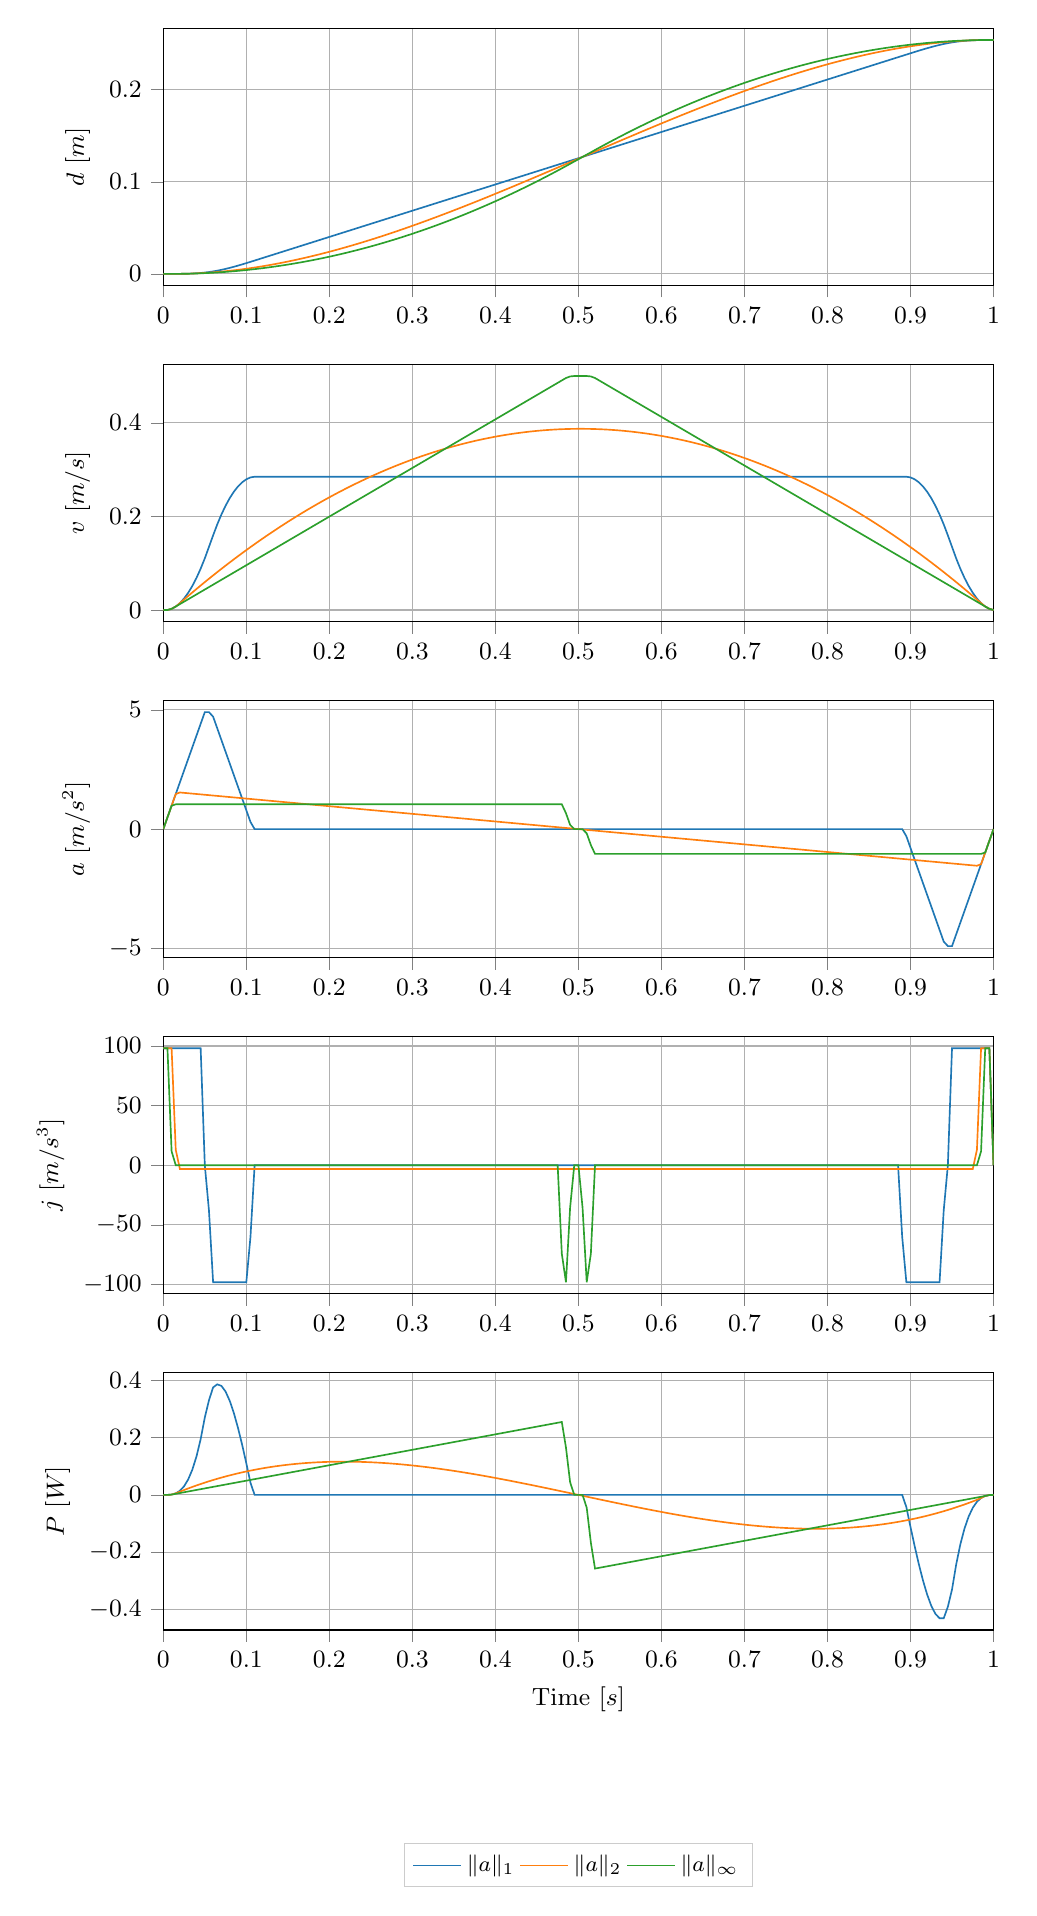
\begin{tikzpicture}

\definecolor{color0}{rgb}{0.12156862745098,0.466666666666667,0.705882352941177}
\definecolor{color1}{rgb}{1,0.498039215686275,0.0549019607843137}
\definecolor{color2}{rgb}{0.172549019607843,0.627450980392157,0.172549019607843}

\begin{groupplot}[group style={group size=1 by 5}]
\nextgroupplot[
tick align=outside,
tick pos=left,
x grid style={white!69.01960784313725!black},
xmajorgrids,
xmin=0, xmax=1,
y grid style={white!69.01960784313725!black},
ylabel={$d$ [$m$]},
ymajorgrids,
ymin=-0.0127, ymax=0.2667
%title = \footnotesize{Acceleration}
]
\addplot [semithick, color0]
table [row sep=\\]{%
0	0 \\
0.005	7.15492698256377e-45 \\
0.01	7.3468396926393e-40 \\
0.015	1.22624999824193e-05 \\
0.02	4.90499999267255e-05 \\
0.025	0.000122624999808562 \\
0.03	0.000245249999598463 \\
0.035	0.000429187499259862 \\
0.04	0.000686699998745778 \\
0.045	0.00103004999799272 \\
0.05	0.00147149999690757 \\
0.055	0.00202331249533063 \\
0.06	0.00269774999283745 \\
0.065	0.00349481248999924 \\
0.07	0.0044097532795291 \\
0.075	0.00543030986184874 \\
0.08	0.0065442197371954 \\
0.085	0.00773922040574979 \\
0.09	0.00900304936767008 \\
0.095	0.0103234441231081 \\
0.1	0.0116881421722219 \\
0.105	0.0130848810151923 \\
0.11	0.0145013981522565 \\
0.115	0.0159254310838363 \\
0.12	0.0173494640157493 \\
0.125	0.0187734969479424 \\
0.13	0.0201975298803767 \\
0.135	0.0216215628130223 \\
0.14	0.0230455957458556 \\
0.145	0.0244696286788575 \\
0.15	0.0258936616120122 \\
0.155	0.0273176945453065 \\
0.16	0.0287417274787289 \\
0.165	0.0301657604122698 \\
0.17	0.0315897933459206 \\
0.175	0.0330138262796738 \\
0.18	0.0344378592135228 \\
0.185	0.0358618921474615 \\
0.19	0.0372859250814848 \\
0.195	0.0387099580155876 \\
0.2	0.0401339909497656 \\
0.205	0.0415580238840149 \\
0.21	0.0429820568183317 \\
0.215	0.0444060897527126 \\
0.22	0.0458301226871546 \\
0.225	0.0472541556216546 \\
0.23	0.0486781885562101 \\
0.235	0.0501022214908184 \\
0.24	0.0515262544254773 \\
0.245	0.0529502873601844 \\
0.25	0.0543743202949379 \\
0.255	0.0557983532297356 \\
0.26	0.0572223861645757 \\
0.265	0.0586464190994565 \\
0.27	0.0600704520343764 \\
0.275	0.0614944849693337 \\
0.28	0.0629185179043269 \\
0.285	0.0643425508393547 \\
0.29	0.0657665837744156 \\
0.295	0.0671906167095084 \\
0.3	0.0686146496446318 \\
0.305	0.0700386825797846 \\
0.31	0.0714627155149657 \\
0.315	0.0728867484501739 \\
0.32	0.0743107813854082 \\
0.325	0.0757348143206676 \\
0.33	0.077158847255951 \\
0.335	0.0785828801912575 \\
0.34	0.0800069131265863 \\
0.345	0.0814309460619363 \\
0.35	0.0828549789973068 \\
0.355	0.0842790119326968 \\
0.36	0.0857030448681056 \\
0.365	0.0871270778035323 \\
0.37	0.0885511107389762 \\
0.375	0.0899751436744365 \\
0.38	0.0913991766099125 \\
0.385	0.0928232095454034 \\
0.39	0.0942472424809086 \\
0.395	0.0956712754164273 \\
0.4	0.0970953083519589 \\
0.405	0.0985193412875027 \\
0.41	0.0999433742230581 \\
0.415	0.101367407158624 \\
0.42	0.102791440094201 \\
0.425	0.104215473029787 \\
0.43	0.105639505965382 \\
0.435	0.107063538900986 \\
0.44	0.108487571836597 \\
0.445	0.109911604772216 \\
0.45	0.111335637707842 \\
0.455	0.112759670643473 \\
0.46	0.11418370357911 \\
0.465	0.115607736514752 \\
0.47	0.117031769450399 \\
0.475	0.118455802386049 \\
0.48	0.119879835321702 \\
0.485	0.121303868257359 \\
0.49	0.122727901193017 \\
0.495	0.124151934128677 \\
0.5	0.125575967064338 \\
0.505	0.127 \\
0.51	0.128424032935662 \\
0.515	0.129848065871323 \\
0.52	0.131272098806983 \\
0.525	0.132696131742641 \\
0.53	0.134120164678298 \\
0.535	0.135544197613951 \\
0.54	0.136968230549601 \\
0.545	0.138392263485248 \\
0.55	0.13981629642089 \\
0.555	0.141240329356527 \\
0.56	0.142664362292158 \\
0.565	0.144088395227784 \\
0.57	0.145512428163403 \\
0.575	0.146936461099014 \\
0.58	0.148360494034618 \\
0.585	0.149784526970213 \\
0.59	0.151208559905799 \\
0.595	0.152632592841376 \\
0.6	0.154056625776942 \\
0.605	0.155480658712497 \\
0.61	0.156904691648041 \\
0.615	0.158328724583573 \\
0.62	0.159752757519091 \\
0.625	0.161176790454597 \\
0.63	0.162600823390087 \\
0.635	0.164024856325563 \\
0.64	0.165448889261024 \\
0.645	0.166872922196468 \\
0.65	0.168296955131894 \\
0.655	0.169720988067303 \\
0.66	0.171145021002693 \\
0.665	0.172569053938064 \\
0.67	0.173993086873414 \\
0.675	0.175417119808742 \\
0.68	0.176841152744049 \\
0.685	0.178265185679332 \\
0.69	0.179689218614592 \\
0.695	0.181113251549826 \\
0.7	0.182537284485034 \\
0.705	0.183961317420215 \\
0.71	0.185385350355368 \\
0.715	0.186809383290492 \\
0.72	0.188233416225584 \\
0.725	0.189657449160645 \\
0.73	0.191081482095673 \\
0.735	0.192505515030666 \\
0.74	0.193929547965624 \\
0.745	0.195353580900543 \\
0.75	0.196777613835424 \\
0.755	0.198201646770264 \\
0.76	0.199625679705062 \\
0.765	0.201049712639816 \\
0.77	0.202473745574523 \\
0.775	0.203897778509182 \\
0.78	0.20532181144379 \\
0.785	0.206745844378345 \\
0.79	0.208169877312845 \\
0.795	0.209593910247287 \\
0.8	0.211017943181668 \\
0.805	0.212441976115985 \\
0.81	0.213866009050234 \\
0.815	0.215290041984412 \\
0.82	0.216714074918515 \\
0.825	0.218138107852538 \\
0.83	0.219562140786477 \\
0.835	0.220986173720326 \\
0.84	0.222410206654079 \\
0.845	0.22383423958773 \\
0.85	0.225258272521271 \\
0.855	0.226682305454694 \\
0.86	0.228106338387988 \\
0.865	0.229530371321143 \\
0.87	0.230954404254144 \\
0.875	0.232378437186978 \\
0.88	0.233802470119623 \\
0.885	0.235226503052058 \\
0.89	0.236650535984251 \\
0.895	0.238074568916164 \\
0.9	0.239498601847743 \\
0.905	0.240915118984808 \\
0.91	0.242311857827778 \\
0.915	0.243676555876892 \\
0.92	0.24499695063233 \\
0.925	0.24626077959425 \\
0.93	0.247455780262805 \\
0.935	0.248569690138151 \\
0.94	0.249590246720471 \\
0.945	0.250505187510001 \\
0.95	0.251302250007163 \\
0.955	0.251976687504669 \\
0.96	0.252528500003092 \\
0.965	0.252969950002007 \\
0.97	0.253313300001254 \\
0.975	0.25357081250074 \\
0.98	0.253754750000402 \\
0.985	0.253877375000191 \\
0.99	0.253950950000073 \\
0.995	0.253987737500018 \\
1	0.254 \\
};
\addplot [semithick, color1]
table [row sep=\\]{%
0	0 \\
0.005	-1.02723585926967e-51 \\
0.01	-1.98932063356359e-51 \\
0.015	1.2262499993547e-05 \\
0.02	4.90499999636167e-05 \\
0.025	0.000122624999768821 \\
0.03	0.000234599927477803 \\
0.035	0.000384574783846816 \\
0.04	0.000572149569625047 \\
0.045	0.000796924285562061 \\
0.05	0.00105849893240768 \\
0.055	0.0013564735109119 \\
0.06	0.00169044802182486 \\
0.065	0.00206002246589679 \\
0.07	0.00246479684387802 \\
0.075	0.00290437115651894 \\
0.08	0.00337834540457 \\
0.085	0.0038863195887817 \\
0.09	0.00442789370990458 \\
0.095	0.00500266776868922 \\
0.1	0.00561024176588622 \\
0.105	0.00625021570224623 \\
0.11	0.00692218957851991 \\
0.115	0.00762576339545796 \\
0.12	0.00836053715381108 \\
0.125	0.00912611085433001 \\
0.13	0.00992208449776549 \\
0.135	0.0107480580848683 \\
0.14	0.0116036316163892 \\
0.145	0.012488405093079 \\
0.15	0.0134019785156886 \\
0.155	0.0143439518849686 \\
0.16	0.0153139252016701 \\
0.165	0.0163114984665437 \\
0.17	0.0173362716803405 \\
0.175	0.0183878448438112 \\
0.18	0.0194658179577067 \\
0.185	0.020569791022778 \\
0.19	0.0216993640397759 \\
0.195	0.0228541370094513 \\
0.2	0.0240337099325553 \\
0.205	0.0252376828098386 \\
0.21	0.0264656556420522 \\
0.215	0.0277172284299471 \\
0.22	0.0289920011742743 \\
0.225	0.0302895738757846 \\
0.23	0.0316095465352292 \\
0.235	0.0329515191533589 \\
0.24	0.0343150917309247 \\
0.245	0.0356998642686777 \\
0.25	0.0371054367673688 \\
0.255	0.0385314092277491 \\
0.26	0.0399773816505695 \\
0.265	0.0414429540365812 \\
0.27	0.0429277263865351 \\
0.275	0.0444312987011823 \\
0.28	0.0459532709812738 \\
0.285	0.0474932432275608 \\
0.29	0.0490508154407941 \\
0.295	0.0506255876217251 \\
0.3	0.0522171597711046 \\
0.305	0.0538251318896838 \\
0.31	0.0554491039782139 \\
0.315	0.0570886760374458 \\
0.32	0.0587434480681308 \\
0.325	0.0604130200710199 \\
0.33	0.0620969920468642 \\
0.335	0.063794963996415 \\
0.34	0.0655065359204233 \\
0.345	0.0672313078196402 \\
0.35	0.068968879694817 \\
0.355	0.0707188515467049 \\
0.36	0.0724808233760549 \\
0.365	0.0742543951836182 \\
0.37	0.0760391669701461 \\
0.375	0.0778347387363897 \\
0.38	0.0796407104831003 \\
0.385	0.0814566822110289 \\
0.39	0.083282253920927 \\
0.395	0.0851170256135456 \\
0.4	0.0869605972896359 \\
0.405	0.0888125689499494 \\
0.41	0.090672540595237 \\
0.415	0.0925401122262502 \\
0.42	0.0944148838437402 \\
0.425	0.0962964554484581 \\
0.43	0.0981844270411554 \\
0.435	0.100078398622583 \\
0.44	0.101977970193493 \\
0.445	0.103882741754636 \\
0.45	0.105792313306763 \\
0.455	0.107706284850625 \\
0.46	0.109624256386975 \\
0.465	0.111545827916563 \\
0.47	0.113470599440141 \\
0.475	0.115398170958459 \\
0.48	0.117328142472269 \\
0.485	0.119260113982323 \\
0.49	0.121193685489372 \\
0.495	0.123128456994167 \\
0.5	0.125064028497459 \\
0.505	0.127 \\
0.51	0.128935971502541 \\
0.515	0.130871543005833 \\
0.52	0.132806314510628 \\
0.525	0.134739886017677 \\
0.53	0.136671857527731 \\
0.535	0.138601829041541 \\
0.54	0.140529400559859 \\
0.545	0.142454172083437 \\
0.55	0.144375743613025 \\
0.555	0.146293715149375 \\
0.56	0.148207686693237 \\
0.565	0.150117258245364 \\
0.57	0.152022029806507 \\
0.575	0.153921601377417 \\
0.58	0.155815572958845 \\
0.585	0.157703544551542 \\
0.59	0.15958511615626 \\
0.595	0.16145988777375 \\
0.6	0.163327459404763 \\
0.605	0.165187431050051 \\
0.61	0.167039402710364 \\
0.615	0.168882974386454 \\
0.62	0.170717746079073 \\
0.625	0.172543317788971 \\
0.63	0.1743592895169 \\
0.635	0.17616526126361 \\
0.64	0.177960833029854 \\
0.645	0.179745604816382 \\
0.65	0.181519176623945 \\
0.655	0.183281148453295 \\
0.66	0.185031120305183 \\
0.665	0.18676869218036 \\
0.67	0.188493464079577 \\
0.675	0.190205036003585 \\
0.68	0.191903007953136 \\
0.685	0.19358697992898 \\
0.69	0.195256551931869 \\
0.695	0.196911323962554 \\
0.7	0.198550896021786 \\
0.705	0.200174868110316 \\
0.71	0.201782840228895 \\
0.715	0.203374412378275 \\
0.72	0.204949184559206 \\
0.725	0.206506756772439 \\
0.73	0.208046729018726 \\
0.735	0.209568701298818 \\
0.74	0.211072273613465 \\
0.745	0.212557045963419 \\
0.75	0.21402261834943 \\
0.755	0.215468590772251 \\
0.76	0.216894563232631 \\
0.765	0.218300135731322 \\
0.77	0.219684908269075 \\
0.775	0.221048480846641 \\
0.78	0.222390453464771 \\
0.785	0.223710426124215 \\
0.79	0.225007998825726 \\
0.795	0.226282771570053 \\
0.8	0.227534344357948 \\
0.805	0.228762317190161 \\
0.81	0.229966290067445 \\
0.815	0.231145862990549 \\
0.82	0.232300635960224 \\
0.825	0.233430208977222 \\
0.83	0.234534182042293 \\
0.835	0.235612155156189 \\
0.84	0.23666372831966 \\
0.845	0.237688501533456 \\
0.85	0.23868607479833 \\
0.855	0.239656048115031 \\
0.86	0.240598021484311 \\
0.865	0.241511594906921 \\
0.87	0.242396368383611 \\
0.875	0.243251941915132 \\
0.88	0.244077915502235 \\
0.885	0.24487388914567 \\
0.89	0.245639462846189 \\
0.895	0.246374236604542 \\
0.9	0.24707781042148 \\
0.905	0.247749784297754 \\
0.91	0.248389758234114 \\
0.915	0.248997332231311 \\
0.92	0.249572106290095 \\
0.925	0.250113680411218 \\
0.93	0.25062165459543 \\
0.935	0.251095628843481 \\
0.94	0.251535203156122 \\
0.945	0.251939977534103 \\
0.95	0.252309551978175 \\
0.955	0.252643526489088 \\
0.96	0.252941501067592 \\
0.965	0.253203075714438 \\
0.97	0.253427850430375 \\
0.975	0.253615425216153 \\
0.98	0.253765400072522 \\
0.985	0.253877375000231 \\
0.99	0.253950950000036 \\
0.995	0.253987737500006 \\
1	0.254 \\
};
\addplot [semithick, color2]
table [row sep=\\]{%
0	0 \\
0.005	-5.33997020257706e-53 \\
0.01	-9.20933114546916e-33 \\
0.015	1.22624989318178e-05 \\
0.02	4.90499946479011e-05 \\
0.025	0.000111816750021611 \\
0.03	0.000200562765006526 \\
0.035	0.000315288039555219 \\
0.04	0.000455992573619226 \\
0.045	0.000622676367149013 \\
0.05	0.000815339420093938 \\
0.055	0.00103398173240222 \\
0.06	0.00127860330402088 \\
0.065	0.00154920413489573 \\
0.07	0.00184578422497131 \\
0.075	0.00216834357419084 \\
0.08	0.00251688218249618 \\
0.085	0.00289140004982781 \\
0.09	0.0032918971761247 \\
0.095	0.00371837356132434 \\
0.1	0.00417082920536263 \\
0.105	0.00464926410817386 \\
0.11	0.00515367826969059 \\
0.115	0.00568407168984365 \\
0.12	0.006240444368562 \\
0.125	0.00682279630577274 \\
0.13	0.00743112750140094 \\
0.135	0.00806543795536964 \\
0.14	0.00872572766759971 \\
0.145	0.00941199663800977 \\
0.15	0.0101242448665161 \\
0.155	0.0108624723530326 \\
0.16	0.0116266790974704 \\
0.165	0.0124168650997383 \\
0.17	0.0132330303597421 \\
0.175	0.0140751748773846 \\
0.18	0.0149432986525657 \\
0.185	0.0158374016851821 \\
0.19	0.016757483975127 \\
0.195	0.0177035455222903 \\
0.2	0.0186755863265579 \\
0.205	0.019673606387812 \\
0.21	0.0206976057059307 \\
0.215	0.0217475842807877 \\
0.22	0.0228235421122522 \\
0.225	0.0239254792001886 \\
0.23	0.0250533955444563 \\
0.235	0.0262072911449091 \\
0.24	0.0273871660013954 \\
0.245	0.0285930201137574 \\
0.25	0.0298248534818311 \\
0.255	0.0310826661054456 \\
0.26	0.0323664579844229 \\
0.265	0.0336762291185772 \\
0.27	0.0350119795077147 \\
0.275	0.0363737091516328 \\
0.28	0.0377614180501196 \\
0.285	0.0391751062029532 \\
0.29	0.0406147736099011 \\
0.295	0.0420804202707191 \\
0.3	0.043572046185151 \\
0.305	0.045089651352927 \\
0.31	0.0466332357737629 \\
0.315	0.0482027994473591 \\
0.32	0.0497983423733991 \\
0.325	0.0514198645515479 \\
0.33	0.0530673659814506 \\
0.335	0.0547408466627305 \\
0.34	0.0564403065949869 \\
0.345	0.0581657457777928 \\
0.35	0.0599171642106924 \\
0.355	0.0616945618931979 \\
0.36	0.0634979388247857 \\
0.365	0.0653272950048932 \\
0.37	0.0671826304329132 \\
0.375	0.0690639451081892 \\
0.38	0.0709712390300088 \\
0.385	0.0729045121975963 \\
0.39	0.0748637646101036 \\
0.395	0.0768489962666002 \\
0.4	0.0788602071660599 \\
0.405	0.0808973973073457 \\
0.41	0.0829605666891906 \\
0.415	0.0850497153101741 \\
0.42	0.0871648431686923 \\
0.425	0.0893059502629202 \\
0.43	0.0914730365907625 \\
0.435	0.0936661021497886 \\
0.44	0.0958851469371454 \\
0.445	0.0981301709494365 \\
0.45	0.100401174182551 \\
0.455	0.102698156631413 \\
0.46	0.1050211182896 \\
0.465	0.107370059148738 \\
0.47	0.109744979197512 \\
0.475	0.112145878419978 \\
0.48	0.114572756792809 \\
0.485	0.117025614282952 \\
0.49	0.119504451004539 \\
0.495	0.122000000341862 \\
0.5	0.124500000205134 \\
0.505	0.127 \\
0.51	0.129499999794866 \\
0.515	0.131999999658138 \\
0.52	0.134495548995461 \\
0.525	0.136974385717048 \\
0.53	0.139427243207191 \\
0.535	0.141854121580022 \\
0.54	0.144255020802488 \\
0.545	0.146629940851262 \\
0.55	0.1489788817104 \\
0.555	0.151301843368587 \\
0.56	0.153598825817449 \\
0.565	0.155869829050564 \\
0.57	0.158114853062855 \\
0.575	0.160333897850211 \\
0.58	0.162526963409238 \\
0.585	0.16469404973708 \\
0.59	0.166835156831308 \\
0.595	0.168950284689826 \\
0.6	0.171039433310809 \\
0.605	0.173102602692654 \\
0.61	0.17513979283394 \\
0.615	0.1771510037334 \\
0.62	0.179136235389896 \\
0.625	0.181095487802404 \\
0.63	0.183028760969991 \\
0.635	0.184936054891811 \\
0.64	0.186817369567087 \\
0.645	0.188672704995107 \\
0.65	0.190502061175214 \\
0.655	0.192305438106802 \\
0.66	0.194082835789308 \\
0.665	0.195834254222207 \\
0.67	0.197559693405013 \\
0.675	0.19925915333727 \\
0.68	0.200932634018549 \\
0.685	0.202580135448452 \\
0.69	0.204201657626601 \\
0.695	0.205797200552641 \\
0.7	0.207366764226237 \\
0.705	0.208910348647073 \\
0.71	0.210427953814849 \\
0.715	0.211919579729281 \\
0.72	0.213385226390099 \\
0.725	0.214824893797047 \\
0.73	0.21623858194988 \\
0.735	0.217626290848367 \\
0.74	0.218988020492285 \\
0.745	0.220323770881423 \\
0.75	0.221633542015577 \\
0.755	0.222917333894554 \\
0.76	0.224175146518169 \\
0.765	0.225406979886243 \\
0.77	0.226612833998605 \\
0.775	0.227792708855091 \\
0.78	0.228946604455544 \\
0.785	0.230074520799811 \\
0.79	0.231176457887748 \\
0.795	0.232252415719212 \\
0.8	0.233302394294069 \\
0.805	0.234326393612188 \\
0.81	0.235324413673442 \\
0.815	0.23629645447771 \\
0.82	0.237242516024873 \\
0.825	0.238162598314818 \\
0.83	0.239056701347434 \\
0.835	0.239924825122615 \\
0.84	0.240766969640258 \\
0.845	0.241583134900262 \\
0.85	0.24237332090253 \\
0.855	0.243137527646967 \\
0.86	0.243875755133484 \\
0.865	0.24458800336199 \\
0.87	0.2452742723324 \\
0.875	0.24593456204463 \\
0.88	0.246568872498599 \\
0.885	0.247177203694227 \\
0.89	0.247759555631438 \\
0.895	0.248315928310156 \\
0.9	0.248846321730309 \\
0.905	0.249350735891826 \\
0.91	0.249829170794637 \\
0.915	0.250281626438676 \\
0.92	0.250708102823875 \\
0.925	0.251108599950172 \\
0.93	0.251483117817504 \\
0.935	0.251831656425809 \\
0.94	0.252154215775029 \\
0.945	0.252450795865104 \\
0.95	0.252721396695979 \\
0.955	0.252966018267598 \\
0.96	0.253184660579906 \\
0.965	0.253377323632851 \\
0.97	0.253544007426381 \\
0.975	0.253684711960445 \\
0.98	0.253799437234993 \\
0.985	0.253888183249978 \\
0.99	0.253950950005352 \\
0.995	0.253987737501068 \\
1	0.254 \\
};
\nextgroupplot[
tick align=outside,
tick pos=left,
x grid style={white!69.01960784313725!black},
xmajorgrids,
xmin=0, xmax=1,
y grid style={white!69.01960784313725!black},
ylabel={$v$ [$m/s$]},
ymajorgrids,
ymin=-0.0249999986327163, ymax=0.524999971287041
]
\addplot [semithick, color0, forget plot]
table [row sep=\\]{%
0	1.43155912149436e-42 \\
0.005	1.41059322098675e-37 \\
0.01	0.00245249999648387 \\
0.015	0.00735749998886123 \\
0.02	0.0147149999763672 \\
0.025	0.0245249999579802 \\
0.03	0.0367874999322799 \\
0.035	0.0515024998971832 \\
0.04	0.0686699998493876 \\
0.045	0.0882899997829714 \\
0.05	0.11036249968461 \\
0.055	0.134887499501365 \\
0.06	0.159412499432357 \\
0.065	0.182988157905972 \\
0.07	0.20411131646393 \\
0.075	0.222781975069331 \\
0.08	0.239000133710879 \\
0.085	0.252765792384056 \\
0.09	0.264078951087597 \\
0.095	0.272939609822767 \\
0.1	0.279347768594083 \\
0.105	0.283303427412843 \\
0.11	0.284806586315947 \\
0.115	0.284806586382605 \\
0.12	0.284806586438632 \\
0.125	0.284806586486858 \\
0.13	0.284806586529116 \\
0.135	0.284806586566658 \\
0.14	0.28480658660038 \\
0.145	0.284806586630943 \\
0.15	0.28480658665885 \\
0.155	0.284806586684492 \\
0.16	0.284806586708179 \\
0.165	0.284806586730161 \\
0.17	0.284806586750641 \\
0.175	0.284806586769791 \\
0.18	0.284806586787751 \\
0.185	0.284806586804642 \\
0.19	0.284806586820565 \\
0.195	0.28480658683561 \\
0.2	0.284806586849852 \\
0.205	0.284806586863358 \\
0.21	0.284806586876186 \\
0.215	0.284806586888388 \\
0.22	0.284806586900009 \\
0.225	0.28480658691109 \\
0.23	0.284806586921667 \\
0.235	0.284806586931773 \\
0.24	0.284806586941436 \\
0.245	0.284806586950684 \\
0.25	0.284806586959541 \\
0.255	0.284806586968027 \\
0.26	0.284806586976164 \\
0.265	0.284806586983969 \\
0.27	0.284806586991459 \\
0.275	0.28480658699865 \\
0.28	0.284806587005554 \\
0.285	0.284806587012186 \\
0.29	0.284806587018557 \\
0.295	0.284806587024679 \\
0.3	0.284806587030561 \\
0.305	0.284806587036213 \\
0.31	0.284806587041644 \\
0.315	0.284806587046861 \\
0.32	0.284806587051874 \\
0.325	0.284806587056688 \\
0.33	0.284806587061311 \\
0.335	0.284806587065748 \\
0.34	0.284806587070006 \\
0.345	0.28480658707409 \\
0.35	0.284806587078005 \\
0.355	0.284806587081755 \\
0.36	0.284806587085345 \\
0.365	0.28480658708878 \\
0.37	0.284806587092063 \\
0.375	0.284806587095197 \\
0.38	0.284806587098187 \\
0.385	0.284806587101035 \\
0.39	0.284806587103745 \\
0.395	0.284806587106319 \\
0.4	0.28480658710876 \\
0.405	0.28480658711107 \\
0.41	0.284806587113251 \\
0.415	0.284806587115306 \\
0.42	0.284806587117237 \\
0.425	0.284806587119046 \\
0.43	0.284806587120733 \\
0.435	0.284806587122302 \\
0.44	0.284806587123752 \\
0.445	0.284806587125086 \\
0.45	0.284806587126305 \\
0.455	0.284806587127409 \\
0.46	0.284806587128401 \\
0.465	0.28480658712928 \\
0.47	0.284806587130047 \\
0.475	0.284806587130704 \\
0.48	0.28480658713125 \\
0.485	0.284806587131687 \\
0.49	0.284806587132014 \\
0.495	0.284806587132232 \\
0.5	0.284806587132341 \\
0.505	0.284806587132341 \\
0.51	0.284806587132232 \\
0.515	0.284806587132014 \\
0.52	0.284806587131687 \\
0.525	0.28480658713125 \\
0.53	0.284806587130704 \\
0.535	0.284806587130047 \\
0.54	0.28480658712928 \\
0.545	0.284806587128401 \\
0.55	0.284806587127409 \\
0.555	0.284806587126305 \\
0.56	0.284806587125086 \\
0.565	0.284806587123752 \\
0.57	0.284806587122302 \\
0.575	0.284806587120733 \\
0.58	0.284806587119046 \\
0.585	0.284806587117237 \\
0.59	0.284806587115306 \\
0.595	0.284806587113251 \\
0.6	0.28480658711107 \\
0.605	0.28480658710876 \\
0.61	0.284806587106319 \\
0.615	0.284806587103745 \\
0.62	0.284806587101035 \\
0.625	0.284806587098187 \\
0.63	0.284806587095197 \\
0.635	0.284806587092063 \\
0.64	0.28480658708878 \\
0.645	0.284806587085345 \\
0.65	0.284806587081755 \\
0.655	0.284806587078005 \\
0.66	0.28480658707409 \\
0.665	0.284806587070006 \\
0.67	0.284806587065748 \\
0.675	0.284806587061311 \\
0.68	0.284806587056688 \\
0.685	0.284806587051874 \\
0.69	0.284806587046861 \\
0.695	0.284806587041644 \\
0.7	0.284806587036213 \\
0.705	0.284806587030561 \\
0.71	0.284806587024679 \\
0.715	0.284806587018557 \\
0.72	0.284806587012186 \\
0.725	0.284806587005554 \\
0.73	0.28480658699865 \\
0.735	0.284806586991459 \\
0.74	0.284806586983969 \\
0.745	0.284806586976164 \\
0.75	0.284806586968027 \\
0.755	0.284806586959541 \\
0.76	0.284806586950684 \\
0.765	0.284806586941436 \\
0.77	0.284806586931773 \\
0.775	0.284806586921667 \\
0.78	0.28480658691109 \\
0.785	0.284806586900009 \\
0.79	0.284806586888388 \\
0.795	0.284806586876186 \\
0.8	0.284806586863358 \\
0.805	0.284806586849852 \\
0.81	0.28480658683561 \\
0.815	0.284806586820565 \\
0.82	0.284806586804642 \\
0.825	0.284806586787751 \\
0.83	0.284806586769791 \\
0.835	0.284806586750641 \\
0.84	0.284806586730161 \\
0.845	0.284806586708179 \\
0.85	0.284806586684492 \\
0.855	0.28480658665885 \\
0.86	0.284806586630943 \\
0.865	0.28480658660038 \\
0.87	0.284806586566658 \\
0.875	0.284806586529116 \\
0.88	0.284806586486858 \\
0.885	0.284806586438632 \\
0.89	0.284806586382605 \\
0.895	0.284806586315947 \\
0.9	0.283303427412843 \\
0.905	0.279347768594083 \\
0.91	0.272939609822767 \\
0.915	0.264078951087597 \\
0.92	0.252765792384056 \\
0.925	0.239000133710879 \\
0.93	0.222781975069331 \\
0.935	0.20411131646393 \\
0.94	0.182988157905972 \\
0.945	0.159412499432357 \\
0.95	0.134887499501365 \\
0.955	0.11036249968461 \\
0.96	0.0882899997829714 \\
0.965	0.0686699998493876 \\
0.97	0.0515024998971832 \\
0.975	0.0367874999322799 \\
0.98	0.0245249999579802 \\
0.985	0.0147149999763672 \\
0.99	0.00735749998886123 \\
0.995	0.00245249999648387 \\
1	0 \\
};
\addplot [semithick, color1, forget plot]
table [row sep=\\]{%
0	0 \\
0.005	0 \\
0.01	0.0024524999987094 \\
0.015	0.00735749999401394 \\
0.02	0.0147149999610408 \\
0.025	0.0223949855417964 \\
0.03	0.0299949712738027 \\
0.035	0.0375149571556461 \\
0.04	0.0449549431874029 \\
0.045	0.0523149293691236 \\
0.05	0.0595949157008442 \\
0.055	0.0667949021825915 \\
0.06	0.0739148888143866 \\
0.065	0.0809548755962463 \\
0.07	0.0879148625281843 \\
0.075	0.0947948496102121 \\
0.08	0.10159483684234 \\
0.085	0.108314824224576 \\
0.09	0.114954811756927 \\
0.095	0.121514799439401 \\
0.1	0.127994787272002 \\
0.105	0.134394775254737 \\
0.11	0.140714763387609 \\
0.115	0.146954751670624 \\
0.12	0.153114740103786 \\
0.125	0.159194728687097 \\
0.13	0.165194717420561 \\
0.135	0.171114706304182 \\
0.14	0.176954695337963 \\
0.145	0.182714684521905 \\
0.15	0.188394673856013 \\
0.155	0.193994663340288 \\
0.16	0.199514652974733 \\
0.165	0.20495464275935 \\
0.17	0.210314632694141 \\
0.175	0.215594622779108 \\
0.18	0.220794613014254 \\
0.185	0.225914603399581 \\
0.19	0.23095459393509 \\
0.195	0.235914584620783 \\
0.2	0.240794575456662 \\
0.205	0.245594566442728 \\
0.21	0.250314557578985 \\
0.215	0.254954548865432 \\
0.22	0.259514540302072 \\
0.225	0.263994531888907 \\
0.23	0.268394523625938 \\
0.235	0.272714515513167 \\
0.24	0.276954507550595 \\
0.245	0.281114499738224 \\
0.25	0.285194492076056 \\
0.255	0.289194484564091 \\
0.26	0.293114477202333 \\
0.265	0.296954469990781 \\
0.27	0.300714462929438 \\
0.275	0.304394456018305 \\
0.28	0.307994449257384 \\
0.285	0.311514442646677 \\
0.29	0.314954436186183 \\
0.295	0.318314429875907 \\
0.3	0.321594423715848 \\
0.305	0.324794417706008 \\
0.31	0.327914411846389 \\
0.315	0.330954406136992 \\
0.32	0.333914400577819 \\
0.325	0.336794395168871 \\
0.33	0.33959438991015 \\
0.335	0.342314384801658 \\
0.34	0.344954379843395 \\
0.345	0.347514375035363 \\
0.35	0.349994370377564 \\
0.355	0.352394365869999 \\
0.36	0.354714361512669 \\
0.365	0.356954357305577 \\
0.37	0.359114353248723 \\
0.375	0.361194349342109 \\
0.38	0.363194345585736 \\
0.385	0.365114341979605 \\
0.39	0.366954338523719 \\
0.395	0.368714335218078 \\
0.4	0.370394332062683 \\
0.405	0.371994329057536 \\
0.41	0.373514326202638 \\
0.415	0.37495432349799 \\
0.42	0.376314320943594 \\
0.425	0.37759431853945 \\
0.43	0.37879431628556 \\
0.435	0.379914314181924 \\
0.44	0.380954312228543 \\
0.445	0.381914310425419 \\
0.45	0.382794308772552 \\
0.455	0.383594307269944 \\
0.46	0.384314305917594 \\
0.465	0.384954304715503 \\
0.47	0.385514303663672 \\
0.475	0.385994302762102 \\
0.48	0.386394302010793 \\
0.485	0.386714301409745 \\
0.49	0.386954300958959 \\
0.495	0.387114300658435 \\
0.5	0.387194300508173 \\
0.505	0.387194300508173 \\
0.51	0.387114300658435 \\
0.515	0.386954300958959 \\
0.52	0.386714301409745 \\
0.525	0.386394302010793 \\
0.53	0.385994302762102 \\
0.535	0.385514303663672 \\
0.54	0.384954304715503 \\
0.545	0.384314305917594 \\
0.55	0.383594307269944 \\
0.555	0.382794308772552 \\
0.56	0.381914310425419 \\
0.565	0.380954312228543 \\
0.57	0.379914314181924 \\
0.575	0.37879431628556 \\
0.58	0.37759431853945 \\
0.585	0.376314320943594 \\
0.59	0.37495432349799 \\
0.595	0.373514326202638 \\
0.6	0.371994329057536 \\
0.605	0.370394332062683 \\
0.61	0.368714335218078 \\
0.615	0.366954338523719 \\
0.62	0.365114341979605 \\
0.625	0.363194345585736 \\
0.63	0.361194349342109 \\
0.635	0.359114353248723 \\
0.64	0.356954357305577 \\
0.645	0.354714361512669 \\
0.65	0.352394365869999 \\
0.655	0.349994370377564 \\
0.66	0.347514375035363 \\
0.665	0.344954379843395 \\
0.67	0.342314384801658 \\
0.675	0.33959438991015 \\
0.68	0.336794395168871 \\
0.685	0.333914400577819 \\
0.69	0.330954406136992 \\
0.695	0.327914411846389 \\
0.7	0.324794417706008 \\
0.705	0.321594423715848 \\
0.71	0.318314429875907 \\
0.715	0.314954436186184 \\
0.72	0.311514442646677 \\
0.725	0.307994449257384 \\
0.73	0.304394456018305 \\
0.735	0.300714462929438 \\
0.74	0.296954469990781 \\
0.745	0.293114477202333 \\
0.75	0.289194484564091 \\
0.755	0.285194492076056 \\
0.76	0.281114499738224 \\
0.765	0.276954507550595 \\
0.77	0.272714515513167 \\
0.775	0.268394523625938 \\
0.78	0.263994531888907 \\
0.785	0.259514540302072 \\
0.79	0.254954548865432 \\
0.795	0.250314557578985 \\
0.8	0.245594566442728 \\
0.805	0.240794575456662 \\
0.81	0.235914584620783 \\
0.815	0.23095459393509 \\
0.82	0.225914603399581 \\
0.825	0.220794613014254 \\
0.83	0.215594622779108 \\
0.835	0.210314632694141 \\
0.84	0.20495464275935 \\
0.845	0.199514652974733 \\
0.85	0.193994663340288 \\
0.855	0.188394673856013 \\
0.86	0.182714684521905 \\
0.865	0.176954695337963 \\
0.87	0.171114706304182 \\
0.875	0.165194717420561 \\
0.88	0.159194728687097 \\
0.885	0.153114740103786 \\
0.89	0.146954751670624 \\
0.895	0.140714763387609 \\
0.9	0.134394775254737 \\
0.905	0.127994787272002 \\
0.91	0.121514799439401 \\
0.915	0.114954811756927 \\
0.92	0.108314824224576 \\
0.925	0.10159483684234 \\
0.93	0.0947948496102121 \\
0.935	0.0879148625281843 \\
0.94	0.0809548755962463 \\
0.945	0.0739148888143866 \\
0.95	0.0667949021825915 \\
0.955	0.0595949157008442 \\
0.96	0.0523149293691236 \\
0.965	0.0449549431874029 \\
0.97	0.0375149571556461 \\
0.975	0.0299949712738027 \\
0.98	0.0223949855417964 \\
0.985	0.0147149999610408 \\
0.99	0.00735749999401394 \\
0.995	0.0024524999987094 \\
1	0 \\
};
\addplot [semithick, color2, forget plot]
table [row sep=\\]{%
0	0 \\
0.005	0 \\
0.01	0.00245249978636357 \\
0.015	0.00735749914321664 \\
0.02	0.0125533510747421 \\
0.025	0.017749202996983 \\
0.03	0.0229450549097385 \\
0.035	0.0281409068128014 \\
0.04	0.0333367587059574 \\
0.045	0.0385326105889851 \\
0.05	0.0437284624616556 \\
0.055	0.0489243143237322 \\
0.06	0.05412016617497 \\
0.065	0.0593160180151155 \\
0.07	0.064511869843906 \\
0.075	0.0697077216610696 \\
0.08	0.0749035734663245 \\
0.085	0.0800994252593784 \\
0.09	0.0852952770399282 \\
0.095	0.0904911288076593 \\
0.1	0.0956869805622451 \\
0.105	0.100882832303346 \\
0.11	0.106078684030611 \\
0.115	0.111274535743671 \\
0.12	0.116470387442147 \\
0.125	0.121666239125641 \\
0.13	0.12686209079374 \\
0.135	0.132057942446013 \\
0.14	0.137253794082012 \\
0.145	0.142449645701267 \\
0.15	0.147645497303291 \\
0.155	0.152841348887572 \\
0.16	0.158037200453578 \\
0.165	0.163233052000749 \\
0.17	0.168428903528502 \\
0.175	0.173624755036225 \\
0.18	0.178820606523278 \\
0.185	0.184016457988988 \\
0.19	0.189212309432649 \\
0.195	0.194408160853521 \\
0.2	0.199604012250825 \\
0.205	0.204799863623739 \\
0.21	0.209995714971402 \\
0.215	0.215191566292904 \\
0.22	0.220387417587283 \\
0.225	0.225583268853527 \\
0.23	0.230779120090563 \\
0.235	0.235974971297257 \\
0.24	0.241170822472408 \\
0.245	0.246366673614741 \\
0.25	0.251562524722902 \\
0.255	0.256758375795454 \\
0.26	0.261954226830864 \\
0.265	0.267150077827499 \\
0.27	0.272345928783617 \\
0.275	0.277541779697356 \\
0.28	0.282737630566721 \\
0.285	0.287933481389572 \\
0.29	0.293129332163615 \\
0.295	0.298325182886376 \\
0.3	0.303521033555192 \\
0.305	0.308716884167187 \\
0.31	0.313912734719246 \\
0.315	0.319108585207993 \\
0.32	0.324304435629758 \\
0.325	0.329500285980541 \\
0.33	0.334696136255976 \\
0.335	0.339891986451276 \\
0.34	0.345087836561189 \\
0.345	0.350283686579925 \\
0.35	0.355479536501085 \\
0.355	0.360675386317573 \\
0.36	0.365871236021489 \\
0.365	0.371067085604004 \\
0.37	0.376262935055208 \\
0.375	0.381458784363924 \\
0.38	0.386654633517488 \\
0.385	0.391850482501466 \\
0.39	0.397046331299313 \\
0.395	0.402242179891939 \\
0.4	0.407438028257158 \\
0.405	0.412633876368981 \\
0.41	0.417829724196695 \\
0.415	0.423025571703643 \\
0.42	0.428221418845586 \\
0.425	0.433417265568458 \\
0.43	0.438613111805221 \\
0.435	0.443808957471356 \\
0.44	0.44900480245822 \\
0.445	0.454200646622928 \\
0.45	0.459396489772415 \\
0.455	0.464592331637337 \\
0.46	0.469788171827677 \\
0.465	0.474984009754743 \\
0.47	0.480179844493135 \\
0.475	0.485375674566265 \\
0.48	0.490571498028534 \\
0.485	0.495767344317467 \\
0.49	0.499109867464693 \\
0.495	0.499999972654325 \\
0.5	0.499999958973193 \\
0.505	0.499999958973193 \\
0.51	0.499999972654325 \\
0.515	0.499109867464689 \\
0.52	0.49576734431746 \\
0.525	0.490571498028533 \\
0.53	0.485375674566264 \\
0.535	0.480179844493135 \\
0.54	0.474984009754743 \\
0.545	0.469788171827677 \\
0.55	0.464592331637337 \\
0.555	0.459396489772415 \\
0.56	0.454200646622928 \\
0.565	0.44900480245822 \\
0.57	0.443808957471356 \\
0.575	0.438613111805221 \\
0.58	0.433417265568458 \\
0.585	0.428221418845586 \\
0.59	0.423025571703643 \\
0.595	0.417829724196695 \\
0.6	0.412633876368981 \\
0.605	0.407438028257158 \\
0.61	0.402242179891939 \\
0.615	0.397046331299313 \\
0.62	0.391850482501466 \\
0.625	0.386654633517488 \\
0.63	0.381458784363924 \\
0.635	0.376262935055208 \\
0.64	0.371067085604004 \\
0.645	0.365871236021489 \\
0.65	0.360675386317573 \\
0.655	0.355479536501085 \\
0.66	0.350283686579925 \\
0.665	0.345087836561189 \\
0.67	0.339891986451276 \\
0.675	0.334696136255976 \\
0.68	0.329500285980541 \\
0.685	0.324304435629758 \\
0.69	0.319108585207993 \\
0.695	0.313912734719246 \\
0.7	0.308716884167187 \\
0.705	0.303521033555192 \\
0.71	0.298325182886376 \\
0.715	0.293129332163615 \\
0.72	0.287933481389572 \\
0.725	0.282737630566721 \\
0.73	0.277541779697356 \\
0.735	0.272345928783617 \\
0.74	0.267150077827499 \\
0.745	0.261954226830864 \\
0.75	0.256758375795454 \\
0.755	0.251562524722902 \\
0.76	0.246366673614741 \\
0.765	0.241170822472408 \\
0.77	0.235974971297257 \\
0.775	0.230779120090563 \\
0.78	0.225583268853527 \\
0.785	0.220387417587283 \\
0.79	0.215191566292904 \\
0.795	0.209995714971402 \\
0.8	0.204799863623739 \\
0.805	0.199604012250825 \\
0.81	0.194408160853521 \\
0.815	0.189212309432649 \\
0.82	0.184016457988988 \\
0.825	0.178820606523278 \\
0.83	0.173624755036225 \\
0.835	0.168428903528502 \\
0.84	0.163233052000749 \\
0.845	0.158037200453578 \\
0.85	0.152841348887572 \\
0.855	0.147645497303291 \\
0.86	0.142449645701267 \\
0.865	0.137253794082012 \\
0.87	0.132057942446013 \\
0.875	0.12686209079374 \\
0.88	0.121666239125641 \\
0.885	0.116470387442147 \\
0.89	0.111274535743671 \\
0.895	0.106078684030611 \\
0.9	0.100882832303346 \\
0.905	0.0956869805622451 \\
0.91	0.0904911288076593 \\
0.915	0.0852952770399282 \\
0.92	0.0800994252593784 \\
0.925	0.0749035734663245 \\
0.93	0.0697077216610696 \\
0.935	0.064511869843906 \\
0.94	0.0593160180151155 \\
0.945	0.05412016617497 \\
0.95	0.0489243143237322 \\
0.955	0.0437284624616556 \\
0.96	0.0385326105889851 \\
0.965	0.0333367587059574 \\
0.97	0.0281409068128014 \\
0.975	0.0229450549097385 \\
0.98	0.017749202996983 \\
0.985	0.0125533510747421 \\
0.99	0.00735749914321664 \\
0.995	0.00245249978636357 \\
1	1.74825809539874e-49 \\
};
\nextgroupplot[
tick align=outside,
tick pos=left,
x grid style={white!69.01960784313725!black},
xmajorgrids,
xmin=0, xmax=1,
y grid style={white!69.01960784313725!black},
ylabel={$a$ [$m/s^2$]},
ymajorgrids,
ymin=-5.39549998481818, ymax=5.39549998481818
]
\addplot [semithick, color0, forget plot]
table [row sep=\\]{%
0	0 \\
0.005	0.490499999296774 \\
0.01	0.980999998475471 \\
0.015	1.4714999975012 \\
0.02	1.96199999632259 \\
0.025	2.45249999485994 \\
0.03	2.94299999298066 \\
0.035	3.43349999044088 \\
0.04	3.92399998671677 \\
0.045	4.41449998032782 \\
0.05	4.90499996335098 \\
0.055	4.90499998619835 \\
0.06	4.71513169472291 \\
0.065	4.22463171159159 \\
0.07	3.73413172108023 \\
0.075	3.24363172830967 \\
0.08	2.75313173463543 \\
0.085	2.26263174070815 \\
0.09	1.77213174703391 \\
0.095	1.28163175426335 \\
0.1	0.791131763751986 \\
0.105	0.300631780620676 \\
0.11	1.33316283769716e-08 \\
0.115	1.12053678774955e-08 \\
0.12	9.64529310023644e-09 \\
0.125	8.45155959515196e-09 \\
0.13	7.50846816724312e-09 \\
0.135	6.74439515869773e-09 \\
0.14	6.11262920627908e-09 \\
0.145	5.58140634252849e-09 \\
0.15	5.12837389989298e-09 \\
0.155	4.73734522420055e-09 \\
0.16	4.39631063109834e-09 \\
0.165	4.09617165088719e-09 \\
0.17	3.82990924606116e-09 \\
0.175	3.59202179574693e-09 \\
0.18	3.37813600769635e-09 \\
0.185	3.18473170941209e-09 \\
0.19	3.00894344147576e-09 \\
0.195	2.84841495905151e-09 \\
0.2	2.70119088167224e-09 \\
0.205	2.56563487750148e-09 \\
0.21	2.44036709808475e-09 \\
0.215	2.32421577854253e-09 \\
0.22	2.21617939744268e-09 \\
0.225	2.11539680273341e-09 \\
0.23	2.02112341347122e-09 \\
0.235	1.93271210288473e-09 \\
0.24	1.84959772246318e-09 \\
0.245	1.77128448283383e-09 \\
0.25	1.69733559447178e-09 \\
0.255	1.62736470970996e-09 \\
0.26	1.56102881084667e-09 \\
0.265	1.49802226700028e-09 \\
0.27	1.4380718415274e-09 \\
0.275	1.38093247715683e-09 \\
0.28	1.32638372099753e-09 \\
0.285	1.27422667880576e-09 \\
0.29	1.22428140921866e-09 \\
0.295	1.17638468546833e-09 \\
0.3	1.1303880654198e-09 \\
0.305	1.08615622141003e-09 \\
0.31	1.0435654898948e-09 \\
0.315	1.00250260778964e-09 \\
0.32	9.62863607966154e-10 \\
0.325	9.24552850906147e-10 \\
0.33	8.87482173230605e-10 \\
0.335	8.51570136873724e-10 \\
0.34	8.16741365191102e-10 \\
0.345	7.8292595437849e-10 \\
0.35	7.50058950313294e-10 \\
0.355	7.18079882380118e-10 \\
0.36	6.86932347055453e-10 \\
0.365	6.56563635046977e-10 \\
0.37	6.26924396643285e-10 \\
0.375	5.97968340657689e-10 \\
0.38	5.69651962967158e-10 \\
0.385	5.41934301172823e-10 \\
0.39	5.14776712356631e-10 \\
0.395	4.88142671292043e-10 \\
0.4	4.61997586795346e-10 \\
0.405	4.36308634186543e-10 \\
0.41	4.1104460207207e-10 \\
0.415	3.86175751871406e-10 \\
0.42	3.61673688691146e-10 \\
0.425	3.37511242307164e-10 \\
0.43	3.13662357151711e-10 \\
0.435	2.90101990320527e-10 \\
0.44	2.66806016717752e-10 \\
0.445	2.43751140545641e-10 \\
0.45	2.20914812423678e-10 \\
0.455	1.98275151488971e-10 \\
0.46	1.75810871888264e-10 \\
0.465	1.53501213122351e-10 \\
0.47	1.31325873747279e-10 \\
0.475	1.09264947974004e-10 \\
0.48	8.72988647399637e-11 \\
0.485	6.54083288527694e-11 \\
0.49	4.35742638283634e-11 \\
0.495	2.17777560639465e-11 \\
0.5	6.79283911244658e-26 \\
0.505	-2.1777756063946e-11 \\
0.51	-4.35742638283633e-11 \\
0.515	-6.54083288527692e-11 \\
0.52	-8.72988647399635e-11 \\
0.525	-1.09264947974004e-10 \\
0.53	-1.31325873747279e-10 \\
0.535	-1.53501213122351e-10 \\
0.54	-1.75810871888263e-10 \\
0.545	-1.98275151488971e-10 \\
0.55	-2.20914812423678e-10 \\
0.555	-2.43751140545641e-10 \\
0.56	-2.66806016717752e-10 \\
0.565	-2.90101990320527e-10 \\
0.57	-3.13662357151711e-10 \\
0.575	-3.37511242307165e-10 \\
0.58	-3.61673688691146e-10 \\
0.585	-3.86175751871406e-10 \\
0.59	-4.1104460207207e-10 \\
0.595	-4.36308634186543e-10 \\
0.6	-4.61997586795346e-10 \\
0.605	-4.88142671292043e-10 \\
0.61	-5.14776712356631e-10 \\
0.615	-5.41934301172823e-10 \\
0.62	-5.69651962967158e-10 \\
0.625	-5.97968340657689e-10 \\
0.63	-6.26924396643285e-10 \\
0.635	-6.56563635046977e-10 \\
0.64	-6.86932347055453e-10 \\
0.645	-7.18079882380118e-10 \\
0.65	-7.50058950313294e-10 \\
0.655	-7.8292595437849e-10 \\
0.66	-8.16741365191102e-10 \\
0.665	-8.51570136873724e-10 \\
0.67	-8.87482173230605e-10 \\
0.675	-9.24552850906147e-10 \\
0.68	-9.62863607966154e-10 \\
0.685	-1.00250260778964e-09 \\
0.69	-1.0435654898948e-09 \\
0.695	-1.08615622141003e-09 \\
0.7	-1.1303880654198e-09 \\
0.705	-1.17638468546833e-09 \\
0.71	-1.22428140921866e-09 \\
0.715	-1.27422667880576e-09 \\
0.72	-1.32638372099753e-09 \\
0.725	-1.38093247715683e-09 \\
0.73	-1.4380718415274e-09 \\
0.735	-1.49802226700028e-09 \\
0.74	-1.56102881084667e-09 \\
0.745	-1.62736470970996e-09 \\
0.75	-1.69733559447178e-09 \\
0.755	-1.77128448283383e-09 \\
0.76	-1.84959772246319e-09 \\
0.765	-1.93271210288472e-09 \\
0.77	-2.02112341347122e-09 \\
0.775	-2.11539680273341e-09 \\
0.78	-2.21617939744267e-09 \\
0.785	-2.32421577854253e-09 \\
0.79	-2.44036709808475e-09 \\
0.795	-2.56563487750147e-09 \\
0.8	-2.70119088167224e-09 \\
0.805	-2.84841495905151e-09 \\
0.81	-3.00894344147575e-09 \\
0.815	-3.18473170941209e-09 \\
0.82	-3.37813600769634e-09 \\
0.825	-3.59202179574692e-09 \\
0.83	-3.82990924606116e-09 \\
0.835	-4.09617165088719e-09 \\
0.84	-4.39631063109833e-09 \\
0.845	-4.73734522420054e-09 \\
0.85	-5.12837389989297e-09 \\
0.855	-5.58140634252849e-09 \\
0.86	-6.11262920627909e-09 \\
0.865	-6.74439515869772e-09 \\
0.87	-7.50846816724311e-09 \\
0.875	-8.45155959515197e-09 \\
0.88	-9.64529310023644e-09 \\
0.885	-1.12053678774955e-08 \\
0.89	-1.33316283769715e-08 \\
0.895	-0.300631780620676 \\
0.9	-0.791131763751986 \\
0.905	-1.28163175426335 \\
0.91	-1.77213174703391 \\
0.915	-2.26263174070815 \\
0.92	-2.75313173463543 \\
0.925	-3.24363172830967 \\
0.93	-3.73413172108023 \\
0.935	-4.22463171159159 \\
0.94	-4.71513169472291 \\
0.945	-4.90499998619835 \\
0.95	-4.90499996335098 \\
0.955	-4.41449998032782 \\
0.96	-3.92399998671677 \\
0.965	-3.43349999044088 \\
0.97	-2.94299999298066 \\
0.975	-2.45249999485994 \\
0.98	-1.96199999632259 \\
0.985	-1.4714999975012 \\
0.99	-0.980999998475471 \\
0.995	-0.490499999296774 \\
1	-1.91101565722546e-39 \\
};
\addplot [semithick, color1, forget plot]
table [row sep=\\]{%
0	0 \\
0.005	0.490499999741881 \\
0.01	0.980999999060907 \\
0.015	1.47149999340537 \\
0.02	1.53599711615111 \\
0.025	1.51999714640126 \\
0.03	1.50399717636868 \\
0.035	1.48799720635136 \\
0.04	1.47199723634414 \\
0.045	1.45599726634411 \\
0.05	1.43999729634947 \\
0.055	1.42399732635902 \\
0.06	1.40799735637193 \\
0.065	1.3919973863876 \\
0.07	1.37599741640558 \\
0.075	1.35999744642552 \\
0.08	1.34399747644716 \\
0.085	1.32799750647028 \\
0.09	1.31199753649471 \\
0.095	1.29599756652031 \\
0.1	1.27999759654695 \\
0.105	1.26399762657454 \\
0.11	1.247997656603 \\
0.115	1.23199768663225 \\
0.12	1.21599771666223 \\
0.125	1.19999774669289 \\
0.13	1.18399777672419 \\
0.135	1.16799780675608 \\
0.14	1.15199783678853 \\
0.145	1.13599786682152 \\
0.15	1.119997896855 \\
0.155	1.10399792688896 \\
0.16	1.08799795692338 \\
0.165	1.07199798695824 \\
0.17	1.05599801699352 \\
0.175	1.03999804702921 \\
0.18	1.02399807706529 \\
0.185	1.00799810710175 \\
0.19	0.991998137138591 \\
0.195	0.97599816717579 \\
0.2	0.959998197213344 \\
0.205	0.943998227251245 \\
0.21	0.927998257289486 \\
0.215	0.911998287328063 \\
0.22	0.89599831736697 \\
0.225	0.879998347406203 \\
0.23	0.863998377445757 \\
0.235	0.847998407485629 \\
0.24	0.831998437525817 \\
0.245	0.815998467566318 \\
0.25	0.79999849760713 \\
0.255	0.78399852764825 \\
0.26	0.767998557689678 \\
0.265	0.751998587731412 \\
0.27	0.735998617773451 \\
0.275	0.719998647815793 \\
0.28	0.703998677858439 \\
0.285	0.687998707901388 \\
0.29	0.671998737944638 \\
0.295	0.655998767988191 \\
0.3	0.639998798032044 \\
0.305	0.623998828076198 \\
0.31	0.607998858120652 \\
0.315	0.591998888165406 \\
0.32	0.575998918210459 \\
0.325	0.55999894825581 \\
0.33	0.543998978301458 \\
0.335	0.527999008347402 \\
0.34	0.511999038393642 \\
0.345	0.495999068440175 \\
0.35	0.479999098486999 \\
0.355	0.463999128534113 \\
0.36	0.447999158581513 \\
0.365	0.431999188629198 \\
0.37	0.415999218677163 \\
0.375	0.399999248725406 \\
0.38	0.383999278773921 \\
0.385	0.367999308822705 \\
0.39	0.351999338871753 \\
0.395	0.335999368921058 \\
0.4	0.319999398970614 \\
0.405	0.303999429020416 \\
0.41	0.287999459070455 \\
0.415	0.271999489120723 \\
0.42	0.255999519171212 \\
0.425	0.239999549221914 \\
0.43	0.223999579272818 \\
0.435	0.207999609323914 \\
0.44	0.191999639375191 \\
0.445	0.175999669426637 \\
0.45	0.159999699478242 \\
0.455	0.143999729529992 \\
0.46	0.127999759581874 \\
0.465	0.111999789633875 \\
0.47	0.0959998196859804 \\
0.475	0.0799998497381768 \\
0.48	0.0639998797904494 \\
0.485	0.0479999098427832 \\
0.49	0.0319999398951631 \\
0.495	0.0159999699475738 \\
0.5	2.74483815952147e-17 \\
0.505	-0.0159999699475738 \\
0.51	-0.031999939895163 \\
0.515	-0.0479999098427831 \\
0.52	-0.0639998797904493 \\
0.525	-0.0799998497381768 \\
0.53	-0.0959998196859803 \\
0.535	-0.111999789633875 \\
0.54	-0.127999759581874 \\
0.545	-0.143999729529992 \\
0.55	-0.159999699478242 \\
0.555	-0.175999669426637 \\
0.56	-0.191999639375191 \\
0.565	-0.207999609323914 \\
0.57	-0.223999579272818 \\
0.575	-0.239999549221914 \\
0.58	-0.255999519171212 \\
0.585	-0.271999489120723 \\
0.59	-0.287999459070454 \\
0.595	-0.303999429020416 \\
0.6	-0.319999398970614 \\
0.605	-0.335999368921058 \\
0.61	-0.351999338871753 \\
0.615	-0.367999308822705 \\
0.62	-0.383999278773921 \\
0.625	-0.399999248725406 \\
0.63	-0.415999218677163 \\
0.635	-0.431999188629198 \\
0.64	-0.447999158581513 \\
0.645	-0.463999128534113 \\
0.65	-0.479999098486999 \\
0.655	-0.495999068440175 \\
0.66	-0.511999038393642 \\
0.665	-0.527999008347402 \\
0.67	-0.543998978301458 \\
0.675	-0.55999894825581 \\
0.68	-0.575998918210459 \\
0.685	-0.591998888165406 \\
0.69	-0.607998858120652 \\
0.695	-0.623998828076198 \\
0.7	-0.639998798032044 \\
0.705	-0.655998767988191 \\
0.71	-0.671998737944638 \\
0.715	-0.687998707901388 \\
0.72	-0.703998677858439 \\
0.725	-0.719998647815793 \\
0.73	-0.735998617773451 \\
0.735	-0.751998587731412 \\
0.74	-0.767998557689678 \\
0.745	-0.78399852764825 \\
0.75	-0.79999849760713 \\
0.755	-0.815998467566318 \\
0.76	-0.831998437525817 \\
0.765	-0.84799840748563 \\
0.77	-0.863998377445757 \\
0.775	-0.879998347406203 \\
0.78	-0.89599831736697 \\
0.785	-0.911998287328063 \\
0.79	-0.927998257289486 \\
0.795	-0.943998227251245 \\
0.8	-0.959998197213344 \\
0.805	-0.97599816717579 \\
0.81	-0.991998137138591 \\
0.815	-1.00799810710175 \\
0.82	-1.02399807706529 \\
0.825	-1.03999804702921 \\
0.83	-1.05599801699352 \\
0.835	-1.07199798695824 \\
0.84	-1.08799795692338 \\
0.845	-1.10399792688896 \\
0.85	-1.119997896855 \\
0.855	-1.13599786682152 \\
0.86	-1.15199783678853 \\
0.865	-1.16799780675608 \\
0.87	-1.18399777672419 \\
0.875	-1.19999774669289 \\
0.88	-1.21599771666223 \\
0.885	-1.23199768663225 \\
0.89	-1.247997656603 \\
0.895	-1.26399762657454 \\
0.9	-1.27999759654695 \\
0.905	-1.29599756652031 \\
0.91	-1.31199753649471 \\
0.915	-1.32799750647028 \\
0.92	-1.34399747644716 \\
0.925	-1.35999744642552 \\
0.93	-1.37599741640558 \\
0.935	-1.3919973863876 \\
0.94	-1.40799735637193 \\
0.945	-1.42399732635902 \\
0.95	-1.43999729634947 \\
0.955	-1.45599726634411 \\
0.96	-1.47199723634414 \\
0.965	-1.48799720635136 \\
0.97	-1.50399717636868 \\
0.975	-1.51999714640126 \\
0.98	-1.53599711615111 \\
0.985	-1.47149999340537 \\
0.99	-0.980999999060907 \\
0.995	-0.490499999741881 \\
1	0 \\
};
\addplot [semithick, color2, forget plot]
table [row sep=\\]{%
0	0 \\
0.005	0.490499957272713 \\
0.01	0.980999871370615 \\
0.015	1.03917038630509 \\
0.02	1.03917038444818 \\
0.025	1.03917038255111 \\
0.03	1.03917038061257 \\
0.035	1.03917037863119 \\
0.04	1.03917037660554 \\
0.045	1.03917037453411 \\
0.05	1.03917037241533 \\
0.055	1.03917037024756 \\
0.06	1.03917036802909 \\
0.065	1.0391703657581 \\
0.07	1.03917036343273 \\
0.075	1.03917036105098 \\
0.08	1.03917035861078 \\
0.085	1.03917035610996 \\
0.09	1.03917035354622 \\
0.095	1.03917035091716 \\
0.1	1.03917034822026 \\
0.105	1.03917034545285 \\
0.11	1.03917034261213 \\
0.115	1.03917033969515 \\
0.12	1.0391703366988 \\
0.125	1.03917033361979 \\
0.13	1.03917033045465 \\
0.135	1.03917032719972 \\
0.14	1.03917032385112 \\
0.145	1.03917032040475 \\
0.15	1.03917031685626 \\
0.155	1.03917031320105 \\
0.16	1.03917030943424 \\
0.165	1.03917030555062 \\
0.17	1.03917030154468 \\
0.175	1.03917029741055 \\
0.18	1.03917029314198 \\
0.185	1.03917028873229 \\
0.19	1.03917028417438 \\
0.195	1.03917027946065 \\
0.2	1.03917027458296 \\
0.205	1.0391702695326 \\
0.21	1.03917026430025 \\
0.215	1.03917025887589 \\
0.22	1.03917025324874 \\
0.225	1.03917024740723 \\
0.23	1.03917024133886 \\
0.235	1.03917023503016 \\
0.24	1.03917022846657 \\
0.245	1.03917022163231 \\
0.25	1.03917021451029 \\
0.255	1.03917020708195 \\
0.26	1.03917019932708 \\
0.265	1.03917019122369 \\
0.27	1.03917018274773 \\
0.275	1.0391701738729 \\
0.28	1.03917016457037 \\
0.285	1.03917015480845 \\
0.29	1.03917014455227 \\
0.295	1.03917013376329 \\
0.3	1.03917012239891 \\
0.305	1.03917011041183 \\
0.31	1.03917009774941 \\
0.315	1.03917008435295 \\
0.32	1.0391700701567 \\
0.325	1.03917005508684 \\
0.33	1.03917003906015 \\
0.335	1.03917002198254 \\
0.34	1.03917000374712 \\
0.345	1.03916998423201 \\
0.35	1.03916996329761 \\
0.355	1.03916994078324 \\
0.36	1.03916991650303 \\
0.365	1.03916989024073 \\
0.37	1.03916986174331 \\
0.375	1.03916983071276 \\
0.38	1.03916979679561 \\
0.385	1.03916975956945 \\
0.39	1.0391697185252 \\
0.395	1.03916967304377 \\
0.4	1.03916962236459 \\
0.405	1.03916956554274 \\
0.41	1.03916950138959 \\
0.415	1.03916942838867 \\
0.42	1.0391693445744 \\
0.425	1.03916924735249 \\
0.43	1.03916913322704 \\
0.435	1.03916899737279 \\
0.44	1.03916883294168 \\
0.445	1.03916862989743 \\
0.45	1.03916837298425 \\
0.455	1.03916803806812 \\
0.46	1.03916758541316 \\
0.465	1.03916694767835 \\
0.47	1.03916601462595 \\
0.475	1.0391646924538 \\
0.48	1.03916925778664 \\
0.485	0.668504629445173 \\
0.49	0.17802103792651 \\
0.495	-2.73622649821273e-06 \\
0.5	1.57924726977116e-20 \\
0.505	2.73622649820289e-06 \\
0.51	-0.178021037927189 \\
0.515	-0.668504629445848 \\
0.52	-1.03916925778546 \\
0.525	-1.03916469245366 \\
0.53	-1.03916601462592 \\
0.535	-1.03916694767835 \\
0.54	-1.03916758541316 \\
0.545	-1.03916803806812 \\
0.55	-1.03916837298425 \\
0.555	-1.03916862989743 \\
0.56	-1.03916883294168 \\
0.565	-1.03916899737279 \\
0.57	-1.03916913322704 \\
0.575	-1.03916924735249 \\
0.58	-1.0391693445744 \\
0.585	-1.03916942838867 \\
0.59	-1.03916950138959 \\
0.595	-1.03916956554274 \\
0.6	-1.03916962236459 \\
0.605	-1.03916967304377 \\
0.61	-1.0391697185252 \\
0.615	-1.03916975956945 \\
0.62	-1.03916979679561 \\
0.625	-1.03916983071276 \\
0.63	-1.03916986174331 \\
0.635	-1.03916989024073 \\
0.64	-1.03916991650303 \\
0.645	-1.03916994078324 \\
0.65	-1.03916996329761 \\
0.655	-1.03916998423201 \\
0.66	-1.03917000374712 \\
0.665	-1.03917002198254 \\
0.67	-1.03917003906015 \\
0.675	-1.03917005508684 \\
0.68	-1.0391700701567 \\
0.685	-1.03917008435295 \\
0.69	-1.03917009774941 \\
0.695	-1.03917011041183 \\
0.7	-1.03917012239891 \\
0.705	-1.03917013376329 \\
0.71	-1.03917014455227 \\
0.715	-1.03917015480845 \\
0.72	-1.03917016457037 \\
0.725	-1.0391701738729 \\
0.73	-1.03917018274773 \\
0.735	-1.03917019122369 \\
0.74	-1.03917019932708 \\
0.745	-1.03917020708195 \\
0.75	-1.03917021451029 \\
0.755	-1.03917022163231 \\
0.76	-1.03917022846657 \\
0.765	-1.03917023503016 \\
0.77	-1.03917024133886 \\
0.775	-1.03917024740723 \\
0.78	-1.03917025324874 \\
0.785	-1.03917025887589 \\
0.79	-1.03917026430025 \\
0.795	-1.0391702695326 \\
0.8	-1.03917027458296 \\
0.805	-1.03917027946065 \\
0.81	-1.03917028417438 \\
0.815	-1.03917028873229 \\
0.82	-1.03917029314198 \\
0.825	-1.03917029741055 \\
0.83	-1.03917030154468 \\
0.835	-1.03917030555062 \\
0.84	-1.03917030943424 \\
0.845	-1.03917031320105 \\
0.85	-1.03917031685626 \\
0.855	-1.03917032040475 \\
0.86	-1.03917032385112 \\
0.865	-1.03917032719972 \\
0.87	-1.03917033045465 \\
0.875	-1.03917033361979 \\
0.88	-1.0391703366988 \\
0.885	-1.03917033969515 \\
0.89	-1.03917034261213 \\
0.895	-1.03917034545285 \\
0.9	-1.03917034822026 \\
0.905	-1.03917035091716 \\
0.91	-1.03917035354622 \\
0.915	-1.03917035610996 \\
0.92	-1.03917035861078 \\
0.925	-1.03917036105098 \\
0.93	-1.03917036343273 \\
0.935	-1.0391703657581 \\
0.94	-1.03917036802909 \\
0.945	-1.03917037024756 \\
0.95	-1.03917037241533 \\
0.955	-1.03917037453411 \\
0.96	-1.03917037660554 \\
0.965	-1.03917037863119 \\
0.97	-1.03917038061257 \\
0.975	-1.03917038255111 \\
0.98	-1.03917038444818 \\
0.985	-1.03917038630509 \\
0.99	-0.980999871370615 \\
0.995	-0.490499957272713 \\
1	-1.6901798905006e-35 \\
};
\nextgroupplot[
tick align=outside,
tick pos=left,
x grid style={white!69.01960784313725!black},
xmajorgrids,
xmin=0, xmax=1,
y grid style={white!69.01960784313725!black},
ylabel={$j$ [$m/s^3$]},
ymajorgrids,
ymin=-107.909998722146, ymax=107.909999885068
]
\addplot [semithick, color0, forget plot]
table [row sep=\\]{%
0	98.0999998593548 \\
0.005	98.0999998357395 \\
0.01	98.0999998051462 \\
0.015	98.0999997642769 \\
0.02	98.0999997074703 \\
0.025	98.099999624145 \\
0.03	98.0999994920429 \\
0.035	98.0999992551775 \\
0.04	98.0999987222103 \\
0.045	98.099996604633 \\
0.05	4.56947296881439e-06 \\
0.055	-37.9736582950882 \\
0.06	-98.0999966262625 \\
0.065	-98.0999981022727 \\
0.07	-98.0999985541125 \\
0.075	-98.0999987348485 \\
0.08	-98.0999987854545 \\
0.085	-98.0999987348484 \\
0.09	-98.0999985541125 \\
0.095	-98.0999981022724 \\
0.1	-98.0999966262621 \\
0.105	-60.1263534578095 \\
0.11	-4.25252099895207e-07 \\
0.115	-3.12014955451816e-07 \\
0.12	-2.38746701016894e-07 \\
0.125	-1.88618285581769e-07 \\
0.13	-1.52814601709078e-07 \\
0.135	-1.26353190483728e-07 \\
0.14	-1.06244572750119e-07 \\
0.145	-9.06064885271019e-08 \\
0.15	-7.82057351384871e-08 \\
0.155	-6.82069186204416e-08 \\
0.16	-6.00277960422306e-08 \\
0.165	-5.32524809652057e-08 \\
0.17	-4.75774900628462e-08 \\
0.175	-4.27771576101152e-08 \\
0.18	-3.86808596568525e-08 \\
0.185	-3.51576535872661e-08 \\
0.19	-3.21056964848493e-08 \\
0.195	-2.94448154758549e-08 \\
0.2	-2.71112008341519e-08 \\
0.205	-2.5053555883345e-08 \\
0.21	-2.32302639084447e-08 \\
0.215	-2.16072762199704e-08 \\
0.22	-2.01565189418524e-08 \\
0.225	-1.88546778524393e-08 \\
0.23	-1.76822621172983e-08 \\
0.235	-1.66228760843083e-08 \\
0.24	-1.5662647925871e-08 \\
0.245	-1.47897776724093e-08 \\
0.25	-1.39941769523646e-08 \\
0.255	-1.32671797726585e-08 \\
0.26	-1.26013087692782e-08 \\
0.265	-1.19900850945755e-08 \\
0.27	-1.14278728741138e-08 \\
0.275	-1.09097512318605e-08 \\
0.28	-1.0431408438354e-08 \\
0.285	-9.98905391741918e-09 \\
0.29	-9.57934475006691e-09 \\
0.295	-9.19932400970606e-09 \\
0.3	-8.84636880195393e-09 \\
0.305	-8.51814630304498e-09 \\
0.31	-8.21257642103274e-09 \\
0.315	-7.92779996469677e-09 \\
0.32	-7.66215141200156e-09 \\
0.325	-7.41413553510833e-09 \\
0.33	-7.18240727137625e-09 \\
0.335	-6.96575433652434e-09 \\
0.34	-6.76308216252247e-09 \\
0.345	-6.57340081303918e-09 \\
0.35	-6.39581358663515e-09 \\
0.355	-6.2295070649329e-09 \\
0.36	-6.07374240169537e-09 \\
0.365	-5.92784768073828e-09 \\
0.37	-5.79121119711916e-09 \\
0.375	-5.66327553810628e-09 \\
0.38	-5.54353235886702e-09 \\
0.385	-5.43151776323845e-09 \\
0.39	-5.32680821291747e-09 \\
0.395	-5.22901689933947e-09 \\
0.4	-5.1377905217605e-09 \\
0.405	-5.05280642289463e-09 \\
0.41	-4.97377004013296e-09 \\
0.415	-4.90041263605185e-09 \\
0.42	-4.83248927679636e-09 \\
0.425	-4.7697770310906e-09 \\
0.43	-4.71207336623685e-09 \\
0.435	-4.65919472055509e-09 \\
0.44	-4.61097523442212e-09 \\
0.445	-4.56726562439262e-09 \\
0.45	-4.52793218694132e-09 \\
0.455	-4.49285592014157e-09 \\
0.46	-4.46193175318256e-09 \\
0.465	-4.43506787501427e-09 \\
0.47	-4.41218515465504e-09 \\
0.475	-4.39321664680811e-09 \\
0.48	-4.37810717743885e-09 \\
0.485	-4.36681300488119e-09 \\
0.49	-4.3593015528834e-09 \\
0.495	-4.35555121278928e-09 \\
0.5	-4.35555121278922e-09 \\
0.505	-4.35930155288346e-09 \\
0.51	-4.36681300488118e-09 \\
0.515	-4.37810717743885e-09 \\
0.52	-4.39321664680811e-09 \\
0.525	-4.41218515465504e-09 \\
0.53	-4.43506787501426e-09 \\
0.535	-4.46193175318257e-09 \\
0.54	-4.49285592014158e-09 \\
0.545	-4.52793218694131e-09 \\
0.55	-4.56726562439267e-09 \\
0.555	-4.61097523442207e-09 \\
0.56	-4.65919472055509e-09 \\
0.565	-4.7120733662368e-09 \\
0.57	-4.7697770310907e-09 \\
0.575	-4.83248927679632e-09 \\
0.58	-4.90041263605187e-09 \\
0.585	-4.97377004013288e-09 \\
0.59	-5.05280642289467e-09 \\
0.595	-5.1377905217605e-09 \\
0.6	-5.22901689933951e-09 \\
0.605	-5.32680821291744e-09 \\
0.61	-5.43151776323842e-09 \\
0.615	-5.54353235886702e-09 \\
0.62	-5.66327553810632e-09 \\
0.625	-5.79121119711914e-09 \\
0.63	-5.92784768073833e-09 \\
0.635	-6.07374240169525e-09 \\
0.64	-6.22950706493296e-09 \\
0.645	-6.39581358663517e-09 \\
0.65	-6.57340081303921e-09 \\
0.655	-6.76308216252244e-09 \\
0.66	-6.96575433652435e-09 \\
0.665	-7.18240727137625e-09 \\
0.67	-7.41413553510834e-09 \\
0.675	-7.66215141200159e-09 \\
0.68	-7.92779996469663e-09 \\
0.685	-8.21257642103288e-09 \\
0.69	-8.51814630304495e-09 \\
0.695	-8.84636880195393e-09 \\
0.7	-9.19932400970606e-09 \\
0.705	-9.57934475006692e-09 \\
0.71	-9.98905391741926e-09 \\
0.715	-1.04314084383539e-08 \\
0.72	-1.09097512318604e-08 \\
0.725	-1.14278728741141e-08 \\
0.73	-1.19900850945754e-08 \\
0.735	-1.2601308769278e-08 \\
0.74	-1.32671797726584e-08 \\
0.745	-1.39941769523648e-08 \\
0.75	-1.47897776724094e-08 \\
0.755	-1.56626479258712e-08 \\
0.76	-1.66228760843079e-08 \\
0.765	-1.76822621172986e-08 \\
0.77	-1.8854677852439e-08 \\
0.775	-2.01565189418523e-08 \\
0.78	-2.16072762199708e-08 \\
0.785	-2.32302639084446e-08 \\
0.79	-2.50535558833446e-08 \\
0.795	-2.71112008341524e-08 \\
0.8	-2.94448154758543e-08 \\
0.805	-3.21056964848493e-08 \\
0.81	-3.51576535872663e-08 \\
0.815	-3.86808596568516e-08 \\
0.82	-4.2777157610116e-08 \\
0.825	-4.75774900628466e-08 \\
0.83	-5.32524809652058e-08 \\
0.835	-6.00277960422298e-08 \\
0.84	-6.82069186204413e-08 \\
0.845	-7.82057351384864e-08 \\
0.85	-9.06064885271038e-08 \\
0.855	-1.0624457275012e-07 \\
0.86	-1.26353190483725e-07 \\
0.865	-1.52814601709079e-07 \\
0.87	-1.88618285581772e-07 \\
0.875	-2.38746701016892e-07 \\
0.88	-3.12014955451818e-07 \\
0.885	-4.25252099895201e-07 \\
0.89	-60.1263534578095 \\
0.895	-98.0999966262621 \\
0.9	-98.0999981022724 \\
0.905	-98.0999985541125 \\
0.91	-98.0999987348484 \\
0.915	-98.0999987854545 \\
0.92	-98.0999987348485 \\
0.925	-98.0999985541125 \\
0.93	-98.0999981022727 \\
0.935	-98.0999966262625 \\
0.94	-37.9736582950882 \\
0.945	4.56947296885282e-06 \\
0.95	98.099996604633 \\
0.955	98.0999987222103 \\
0.96	98.0999992551775 \\
0.965	98.0999994920429 \\
0.97	98.099999624145 \\
0.975	98.0999997074703 \\
0.98	98.0999997642769 \\
0.985	98.0999998051462 \\
0.99	98.0999998357395 \\
0.995	98.0999998593548 \\
1	0 \\
};
\addplot [semithick, color1, forget plot]
table [row sep=\\]{%
0	98.0999999483762 \\
0.005	98.0999998638052 \\
0.01	98.0999988688935 \\
0.015	12.8994245491479 \\
0.02	-3.19999394997009 \\
0.025	-3.19999400651646 \\
0.03	-3.19999400346405 \\
0.035	-3.19999400144375 \\
0.04	-3.19999400000575 \\
0.045	-3.19999399892857 \\
0.05	-3.1999939980902 \\
0.055	-3.1999939974181 \\
0.06	-3.19999399686623 \\
0.065	-3.19999399640434 \\
0.07	-3.19999399601125 \\
0.075	-3.19999399567198 \\
0.08	-3.19999399537566 \\
0.085	-3.1999939951141 \\
0.09	-3.19999399488099 \\
0.095	-3.19999399467149 \\
0.1	-3.19999399448173 \\
0.105	-3.19999399430872 \\
0.11	-3.19999399414998 \\
0.115	-3.1999939940034 \\
0.12	-3.19999399386737 \\
0.125	-3.19999399374046 \\
0.13	-3.19999399362156 \\
0.135	-3.19999399350956 \\
0.14	-3.19999399340372 \\
0.145	-3.19999399330329 \\
0.15	-3.19999399320757 \\
0.155	-3.19999399311606 \\
0.16	-3.19999399302835 \\
0.165	-3.19999399294393 \\
0.17	-3.19999399286246 \\
0.175	-3.1999939927836 \\
0.18	-3.19999399270713 \\
0.185	-3.19999399263273 \\
0.19	-3.19999399256016 \\
0.195	-3.19999399248924 \\
0.2	-3.1999939924198 \\
0.205	-3.19999399235163 \\
0.21	-3.19999399228462 \\
0.215	-3.19999399221861 \\
0.22	-3.19999399215351 \\
0.225	-3.19999399208916 \\
0.23	-3.19999399202548 \\
0.235	-3.19999399196242 \\
0.24	-3.19999399189982 \\
0.245	-3.19999399183768 \\
0.25	-3.19999399177592 \\
0.255	-3.19999399171443 \\
0.26	-3.19999399165325 \\
0.265	-3.19999399159226 \\
0.27	-3.19999399153147 \\
0.275	-3.19999399147081 \\
0.28	-3.19999399141027 \\
0.285	-3.19999399134988 \\
0.29	-3.19999399128955 \\
0.295	-3.19999399122934 \\
0.3	-3.1999939911692 \\
0.305	-3.19999399110919 \\
0.31	-3.19999399104924 \\
0.315	-3.19999399098943 \\
0.32	-3.19999399092981 \\
0.325	-3.19999399087035 \\
0.33	-3.1999939908111 \\
0.335	-3.19999399075212 \\
0.34	-3.19999399069344 \\
0.345	-3.19999399063514 \\
0.35	-3.19999399057727 \\
0.355	-3.19999399051988 \\
0.36	-3.19999399046308 \\
0.365	-3.19999399040691 \\
0.37	-3.19999399035149 \\
0.375	-3.19999399029688 \\
0.38	-3.1999939902432 \\
0.385	-3.19999399019053 \\
0.39	-3.19999399013898 \\
0.395	-3.19999399008869 \\
0.4	-3.19999399003973 \\
0.405	-3.19999398999223 \\
0.41	-3.19999398994632 \\
0.415	-3.19999398990209 \\
0.42	-3.1999939898597 \\
0.425	-3.19999398981923 \\
0.43	-3.19999398978083 \\
0.435	-3.1999939897446 \\
0.44	-3.19999398971065 \\
0.445	-3.1999939896791 \\
0.45	-3.19999398965005 \\
0.455	-3.19999398962359 \\
0.46	-3.19999398959983 \\
0.465	-3.19999398957884 \\
0.47	-3.19999398956071 \\
0.475	-3.19999398954549 \\
0.48	-3.19999398953324 \\
0.485	-3.19999398952402 \\
0.49	-3.19999398951785 \\
0.495	-3.19999398951476 \\
0.5	-3.19999398951476 \\
0.505	-3.19999398951785 \\
0.51	-3.19999398952402 \\
0.515	-3.19999398953324 \\
0.52	-3.19999398954549 \\
0.525	-3.19999398956071 \\
0.53	-3.19999398957884 \\
0.535	-3.19999398959983 \\
0.54	-3.19999398962359 \\
0.545	-3.19999398965005 \\
0.55	-3.1999939896791 \\
0.555	-3.19999398971065 \\
0.56	-3.1999939897446 \\
0.565	-3.19999398978083 \\
0.57	-3.19999398981923 \\
0.575	-3.1999939898597 \\
0.58	-3.1999939899021 \\
0.585	-3.19999398994631 \\
0.59	-3.19999398999223 \\
0.595	-3.19999399003973 \\
0.6	-3.1999939900887 \\
0.605	-3.19999399013898 \\
0.61	-3.19999399019053 \\
0.615	-3.1999939902432 \\
0.62	-3.19999399029688 \\
0.625	-3.19999399035149 \\
0.63	-3.19999399040691 \\
0.635	-3.19999399046307 \\
0.64	-3.1999939905199 \\
0.645	-3.19999399057727 \\
0.65	-3.19999399063514 \\
0.655	-3.19999399069344 \\
0.66	-3.19999399075214 \\
0.665	-3.19999399081108 \\
0.67	-3.19999399087035 \\
0.675	-3.19999399092981 \\
0.68	-3.19999399098945 \\
0.685	-3.19999399104922 \\
0.69	-3.19999399110918 \\
0.695	-3.1999939911692 \\
0.7	-3.19999399122935 \\
0.705	-3.19999399128956 \\
0.71	-3.19999399134988 \\
0.715	-3.19999399141028 \\
0.72	-3.19999399147081 \\
0.725	-3.19999399153147 \\
0.73	-3.19999399159226 \\
0.735	-3.19999399165325 \\
0.74	-3.19999399171445 \\
0.745	-3.19999399177591 \\
0.75	-3.19999399183768 \\
0.755	-3.19999399189982 \\
0.76	-3.19999399196242 \\
0.765	-3.19999399202548 \\
0.77	-3.19999399208915 \\
0.775	-3.19999399215351 \\
0.78	-3.19999399221862 \\
0.785	-3.19999399228462 \\
0.79	-3.19999399235163 \\
0.795	-3.1999939924198 \\
0.8	-3.19999399248924 \\
0.805	-3.19999399256016 \\
0.81	-3.19999399263273 \\
0.815	-3.19999399270713 \\
0.82	-3.19999399278362 \\
0.825	-3.19999399286245 \\
0.83	-3.19999399294393 \\
0.835	-3.19999399302835 \\
0.84	-3.19999399311606 \\
0.845	-3.19999399320757 \\
0.85	-3.19999399330329 \\
0.855	-3.19999399340372 \\
0.86	-3.19999399350956 \\
0.865	-3.19999399362156 \\
0.87	-3.19999399374046 \\
0.875	-3.19999399386737 \\
0.88	-3.19999399400342 \\
0.885	-3.19999399414996 \\
0.89	-3.19999399430872 \\
0.895	-3.19999399448173 \\
0.9	-3.19999399467149 \\
0.905	-3.19999399488099 \\
0.91	-3.1999939951141 \\
0.915	-3.19999399537566 \\
0.92	-3.19999399567198 \\
0.925	-3.19999399601125 \\
0.93	-3.19999399640434 \\
0.935	-3.19999399686623 \\
0.94	-3.1999939974181 \\
0.945	-3.1999939980902 \\
0.95	-3.19999399892857 \\
0.955	-3.19999400000575 \\
0.96	-3.19999400144375 \\
0.965	-3.19999400346405 \\
0.97	-3.19999400651645 \\
0.975	-3.19999394997011 \\
0.98	12.8994245491479 \\
0.985	98.0999988688935 \\
0.99	98.0999998638052 \\
0.995	98.0999999483762 \\
1	0 \\
};
\addplot [semithick, color2, forget plot]
table [row sep=\\]{%
0	98.0999914545427 \\
0.005	98.0999828195804 \\
0.01	11.6341029868945 \\
0.015	-3.71381296465977e-07 \\
0.02	-3.79414323204131e-07 \\
0.025	-3.87707552838176e-07 \\
0.03	-3.96275616571351e-07 \\
0.035	-4.05130975556551e-07 \\
0.04	-4.14286481510757e-07 \\
0.045	-4.23755819962041e-07 \\
0.05	-4.33553509905864e-07 \\
0.055	-4.43694896714074e-07 \\
0.06	-4.54196482188129e-07 \\
0.065	-4.65075375217319e-07 \\
0.07	-4.76349892537903e-07 \\
0.075	-4.88039449808545e-07 \\
0.08	-5.00164653390801e-07 \\
0.085	-5.12747420026897e-07 \\
0.09	-5.25811069144592e-07 \\
0.095	-5.39380422150213e-07 \\
0.1	-5.5348192100653e-07 \\
0.105	-5.68143759133951e-07 \\
0.11	-5.83396021601829e-07 \\
0.115	-5.99270839524898e-07 \\
0.12	-6.15802559802757e-07 \\
0.125	-6.33027930995931e-07 \\
0.13	-6.50986307564199e-07 \\
0.135	-6.69719874833224e-07 \\
0.14	-6.89273897077717e-07 \\
0.145	-7.09696991379404e-07 \\
0.15	-7.3104143030544e-07 \\
0.155	-7.53363476900579e-07 \\
0.16	-7.76723755990371e-07 \\
0.165	-8.01187666368967e-07 \\
0.17	-8.26825839107761e-07 \\
0.175	-8.53714647990726e-07 \\
0.18	-8.819367789785e-07 \\
0.185	-9.11581866647605e-07 \\
0.19	-9.42747206772787e-07 \\
0.195	-9.75538555654405e-07 \\
0.2	-1.01007102847878e-06 \\
0.205	-1.04647011099255e-06 \\
0.21	-1.0848728011279e-06 \\
0.215	-1.12542890001689e-06 \\
0.22	-1.16830247516426e-06 \\
0.225	-1.21367352252843e-06 \\
0.23	-1.26173985902737e-06 \\
0.235	-1.31271928271463e-06 \\
0.24	-1.36685204477859e-06 \\
0.245	-1.42440368588023e-06 \\
0.25	-1.48566829950776e-06 \\
0.255	-1.550972297423e-06 \\
0.26	-1.62067876746665e-06 \\
0.265	-1.69519253266977e-06 \\
0.27	-1.77496604369671e-06 \\
0.275	-1.86050626527765e-06 \\
0.28	-1.95238275297751e-06 \\
0.285	-2.0512371613662e-06 \\
0.29	-2.15779448097159e-06 \\
0.295	-2.27287637273679e-06 \\
0.3	-2.39741705959449e-06 \\
0.305	-2.5324823512964e-06 \\
0.31	-2.67929252895673e-06 \\
0.315	-2.83925001100661e-06 \\
0.32	-3.0139729775824e-06 \\
0.325	-3.20533646678461e-06 \\
0.33	-3.41552290293604e-06 \\
0.335	-3.64708461500689e-06 \\
0.34	-3.90302171104142e-06 \\
0.345	-4.1868797753762e-06 \\
0.35	-4.50287337115175e-06 \\
0.355	-4.85604343969468e-06 \\
0.36	-5.25245965695581e-06 \\
0.365	-5.69948303773023e-06 \\
0.37	-6.20611018856752e-06 \\
0.375	-6.78342956381825e-06 \\
0.38	-7.44523340579468e-06 \\
0.385	-8.20884922228815e-06 \\
0.39	-9.09628574942014e-06 \\
0.395	-1.01358372307204e-05 \\
0.4	-1.13643683496969e-05 \\
0.405	-1.28306312150082e-05 \\
0.41	-1.46001834935379e-05 \\
0.415	-1.67628545125792e-05 \\
0.42	-1.94443819022824e-05 \\
0.425	-2.28250892002457e-05 \\
0.43	-2.71708500348386e-05 \\
0.435	-3.28862222348514e-05 \\
0.44	-4.0608849494456e-05 \\
0.445	-5.13826367486216e-05 \\
0.45	-6.69832262855107e-05 \\
0.455	-9.05309919830731e-05 \\
0.46	-0.000127546960818679 \\
0.465	-0.000186610481361387 \\
0.47	-0.00026443442951659 \\
0.475	0.000913066567415077 \\
0.48	-74.1329256682927 \\
0.485	-98.0967183037327 \\
0.49	-35.6047548306015 \\
0.495	0.00054724529964255 \\
0.5	0.000547245299640574 \\
0.505	-35.6047548307374 \\
0.51	-98.0967183037319 \\
0.515	-74.1329256679226 \\
0.52	0.000913066360255982 \\
0.525	-0.0002644344516919 \\
0.53	-0.000186610485720336 \\
0.535	-0.000127546961844232 \\
0.54	-9.05309922440362e-05 \\
0.545	-6.69832263553455e-05 \\
0.55	-5.13826367686435e-05 \\
0.555	-4.06088495009628e-05 \\
0.56	-3.28862222374163e-05 \\
0.565	-2.71708500360823e-05 \\
0.57	-2.28250892009428e-05 \\
0.575	-1.9444381902699e-05 \\
0.58	-1.67628545128302e-05 \\
0.585	-1.46001834936859e-05 \\
0.59	-1.28306312150919e-05 \\
0.595	-1.13643683497416e-05 \\
0.6	-1.01358372307422e-05 \\
0.605	-9.09628574942948e-06 \\
0.61	-8.20884922229108e-06 \\
0.615	-7.44523340579461e-06 \\
0.62	-6.78342956381706e-06 \\
0.625	-6.20611018856618e-06 \\
0.63	-5.6994830377291e-06 \\
0.635	-5.25245965695504e-06 \\
0.64	-4.85604343969429e-06 \\
0.645	-4.50287337115168e-06 \\
0.65	-4.18687977537638e-06 \\
0.655	-3.90302171104179e-06 \\
0.66	-3.6470846150074e-06 \\
0.665	-3.41552290293662e-06 \\
0.67	-3.20533646678523e-06 \\
0.675	-3.01397297758302e-06 \\
0.68	-2.83925001100719e-06 \\
0.685	-2.67929252895727e-06 \\
0.69	-2.53248235129687e-06 \\
0.695	-2.39741705959489e-06 \\
0.7	-2.27287637273711e-06 \\
0.705	-2.15779448097181e-06 \\
0.71	-2.05123716136637e-06 \\
0.715	-1.95238275297757e-06 \\
0.72	-1.86050626527767e-06 \\
0.725	-1.77496604369664e-06 \\
0.73	-1.69519253266966e-06 \\
0.735	-1.62067876746649e-06 \\
0.74	-1.55097229742277e-06 \\
0.745	-1.48566829950749e-06 \\
0.75	-1.42440368587994e-06 \\
0.755	-1.36685204477826e-06 \\
0.76	-1.31271928271429e-06 \\
0.765	-1.26173985902701e-06 \\
0.77	-1.21367352252805e-06 \\
0.775	-1.16830247516387e-06 \\
0.78	-1.12542890001649e-06 \\
0.785	-1.0848728011275e-06 \\
0.79	-1.04647011099215e-06 \\
0.795	-1.01007102847838e-06 \\
0.8	-9.75538555653996e-07 \\
0.805	-9.42747206772386e-07 \\
0.81	-9.1158186664721e-07 \\
0.815	-8.81936778978104e-07 \\
0.82	-8.53714647990335e-07 \\
0.825	-8.26825839107376e-07 \\
0.83	-8.01187666368599e-07 \\
0.835	-7.76723755989991e-07 \\
0.84	-7.53363476900216e-07 \\
0.845	-7.3104143030508e-07 \\
0.85	-7.09696991379058e-07 \\
0.855	-6.89273897077375e-07 \\
0.86	-6.69719874832887e-07 \\
0.865	-6.50986307563889e-07 \\
0.87	-6.33027930995618e-07 \\
0.875	-6.15802559802473e-07 \\
0.88	-5.9927083952461e-07 \\
0.885	-5.8339602160156e-07 \\
0.89	-5.68143759133702e-07 \\
0.895	-5.53481921006299e-07 \\
0.9	-5.39380422149984e-07 \\
0.905	-5.25811069144381e-07 \\
0.91	-5.12747420026711e-07 \\
0.915	-5.0016465339062e-07 \\
0.92	-4.88039449808379e-07 \\
0.925	-4.76349892537749e-07 \\
0.93	-4.65075375217184e-07 \\
0.935	-4.54196482188015e-07 \\
0.94	-4.43694896713973e-07 \\
0.945	-4.335535099058e-07 \\
0.95	-4.23755819962003e-07 \\
0.955	-4.14286481510733e-07 \\
0.96	-4.05130975556532e-07 \\
0.965	-3.96275616571313e-07 \\
0.97	-3.87707552838138e-07 \\
0.975	-3.7941432320412e-07 \\
0.98	-3.71381296465594e-07 \\
0.985	11.6341029868945 \\
0.99	98.0999828195804 \\
0.995	98.0999914545427 \\
1	0 \\
};
\nextgroupplot[
legend cell align={left},
legend entries={{\footnotesize{$\|a\|_1$}},{\footnotesize{$\|a\|_2$}},{\footnotesize{$\|a\|_\infty$}}},
legend style={at={(0.5,-1.0)}, anchor=south, draw=white!80.0!black},
legend columns=3,
tick align=outside,
tick pos=left,
x grid style={white!69.01960784313725!black},
ylabel={$P$ [$W$]},
xmajorgrids,
xmin=0, xmax=1,
y grid style={white!69.01960784313725!black},
xlabel={Time [$s$]},
ymajorgrids,
ymin=-0.472303402496621, ymax=0.427425558313567
]
\addlegendimage{no markers, color0}
\addlegendimage{no markers, color1}
\addlegendimage{no markers, color2}
\addplot [semithick, color0, forget plot]
table [row sep=\\]{%
0	0 \\
0.005	3.45947986951016e-38 \\
0.01	0.00120295124640588 \\
0.015	0.0054132806076122 \\
0.02	0.0144354149497597 \\
0.025	0.0300737811354432 \\
0.03	0.0541328060212379 \\
0.035	0.0884169164523299 \\
0.04	0.134730539248419 \\
0.045	0.194878101152535 \\
0.05	0.270664028454169 \\
0.055	0.330811591596263 \\
0.06	0.375825464304252 \\
0.065	0.386528787367649 \\
0.07	0.381089270719703 \\
0.075	0.361311341415187 \\
0.08	0.328999426350766 \\
0.085	0.285957952406706 \\
0.09	0.233991346472873 \\
0.095	0.174904035472553 \\
0.1	0.110500446434009 \\
0.105	0.0425850069195317 \\
0.11	1.89846778403904e-09 \\
0.115	1.5956812871754e-09 \\
0.12	1.37352150153921e-09 \\
0.125	1.20352991939274e-09 \\
0.13	1.06923059438752e-09 \\
0.135	9.60424081802697e-10 \\
0.14	8.70458529697069e-10 \\
0.145	7.94810644507919e-10 \\
0.15	7.30297332769428e-10 \\
0.155	6.74613561625319e-10 \\
0.16	6.26049112475999e-10 \\
0.165	5.83308333275013e-10 \\
0.17	5.453916899677e-10 \\
0.175	5.11515733624688e-10 \\
0.18	4.81057693028399e-10 \\
0.185	4.53516284023084e-10 \\
0.19	4.28483455751418e-10 \\
0.195	4.05623671189477e-10 \\
0.2	3.84658477719506e-10 \\
0.205	3.65354856299393e-10 \\
0.21	3.47516311965231e-10 \\
0.215	3.30975981539418e-10 \\
0.22	3.15591245071884e-10 \\
0.225	3.01239471674568e-10 \\
0.23	2.87814630569103e-10 \\
0.235	2.75224568772164e-10 \\
0.24	2.63388807274697e-10 \\
0.245	2.52236744037305e-10 \\
0.25	2.41706178793226e-10 \\
0.255	2.31742094362354e-10 \\
0.26	2.2229564389435e-10 \\
0.265	2.13323304545169e-10 \\
0.27	2.04786166516971e-10 \\
0.275	1.96649332847314e-10 \\
0.28	1.88881410318517e-10 \\
0.285	1.81454075735271e-10 \\
0.29	1.74341704854918e-10 \\
0.295	1.67521053648167e-10 \\
0.3	1.60970983466145e-10 \\
0.305	1.54672223203969e-10 \\
0.31	1.4860716276569e-10 \\
0.315	1.42759673115073e-10 \\
0.32	1.37114948990647e-10 \\
0.325	1.31659371010055e-10 \\
0.33	1.26380384417782e-10 \\
0.335	1.21266392165059e-10 \\
0.34	1.16306660369488e-10 \\
0.345	1.11491234499131e-10 \\
0.35	1.0681086487302e-10 \\
0.355	1.02256940276375e-10 \\
0.36	9.78214286616948e-11 \\
0.365	9.34968240521663e-11 \\
0.37	8.92760988863624e-11 \\
0.375	8.51526611468474e-11 \\
0.38	8.11203157032296e-11 \\
0.385	7.71732293750082e-11 \\
0.39	7.33058992833892e-11 \\
0.395	6.95131241158243e-11 \\
0.4	6.57899779738327e-11 \\
0.405	6.21317865148808e-11 \\
0.41	5.85341051337354e-11 \\
0.415	5.49926989585912e-11 \\
0.42	5.15035244631138e-11 \\
0.425	4.80627125179064e-11 \\
0.43	4.46665527243117e-11 \\
0.435	4.13114788902882e-11 \\
0.44	3.79940555227328e-11 \\
0.445	3.47109652233256e-11 \\
0.45	3.14589968860178e-11 \\
0.455	2.8235034603872e-11 \\
0.46	2.50360472012824e-11 \\
0.465	2.18590783147905e-11 \\
0.47	1.87012369519171e-11 \\
0.475	1.5559688462745e-11 \\
0.48	1.24316458635108e-11 \\
0.485	9.31436145527215e-12 \\
0.49	6.20511868387308e-12 \\
0.495	3.10122418998543e-12 \\
0.5	9.67322662277494e-27 \\
0.505	-3.10122418998655e-12 \\
0.51	-6.20511868387781e-12 \\
0.515	-9.31436145528282e-12 \\
0.52	-1.24316458635299e-11 \\
0.525	-1.55596884627749e-11 \\
0.53	-1.87012369519602e-11 \\
0.535	-2.18590783148494e-11 \\
0.54	-2.50360472013597e-11 \\
0.545	-2.82350346039703e-11 \\
0.55	-3.14589968861398e-11 \\
0.555	-3.47109652234742e-11 \\
0.56	-3.79940555229108e-11 \\
0.565	-4.13114788904985e-11 \\
0.57	-4.46665527245576e-11 \\
0.575	-4.80627125181912e-11 \\
0.58	-5.15035244634408e-11 \\
0.585	-5.49926989589641e-11 \\
0.59	-5.85341051341577e-11 \\
0.595	-6.21317865153567e-11 \\
0.6	-6.57899779743663e-11 \\
0.605	-6.951312411642e-11 \\
0.61	-7.33058992840516e-11 \\
0.615	-7.71732293757424e-11 \\
0.62	-8.11203157040408e-11 \\
0.625	-8.51526611477413e-11 \\
0.63	-8.92760988873449e-11 \\
0.635	-9.3496824053244e-11 \\
0.64	-9.78214286628744e-11 \\
0.645	-1.02256940277664e-10 \\
0.65	-1.06810864874426e-10 \\
0.655	-1.11491234500664e-10 \\
0.66	-1.16306660371155e-10 \\
0.665	-1.21266392166872e-10 \\
0.67	-1.26380384419751e-10 \\
0.675	-1.31659371012192e-10 \\
0.68	-1.37114948992965e-10 \\
0.685	-1.42759673117585e-10 \\
0.69	-1.48607162768412e-10 \\
0.695	-1.54672223206919e-10 \\
0.7	-1.6097098346934e-10 \\
0.705	-1.67521053651627e-10 \\
0.71	-1.74341704858666e-10 \\
0.715	-1.8145407573933e-10 \\
0.72	-1.88881410322915e-10 \\
0.725	-1.96649332852081e-10 \\
0.73	-2.04786166522141e-10 \\
0.735	-2.13323304550779e-10 \\
0.74	-2.22295643900442e-10 \\
0.745	-2.31742094368975e-10 \\
0.75	-2.41706178800428e-10 \\
0.755	-2.52236744045149e-10 \\
0.76	-2.63388807283249e-10 \\
0.765	-2.75224568781502e-10 \\
0.77	-2.87814630579316e-10 \\
0.775	-3.01239471685755e-10 \\
0.78	-3.15591245084162e-10 \\
0.785	-3.30975981552923e-10 \\
0.79	-3.47516311980119e-10 \\
0.795	-3.65354856315849e-10 \\
0.8	-3.84658477737747e-10 \\
0.805	-4.05623671209761e-10 \\
0.81	-4.28483455774052e-10 \\
0.815	-4.5351628404844e-10 \\
0.82	-4.81057693056927e-10 \\
0.825	-5.11515733656945e-10 \\
0.83	-5.45391690004371e-10 \\
0.835	-5.83308333316959e-10 \\
0.84	-6.26049112524317e-10 \\
0.845	-6.74613561681424e-10 \\
0.85	-7.30297332835178e-10 \\
0.855	-7.94810644585799e-10 \\
0.86	-8.70458529790481e-10 \\
0.865	-9.60424081916413e-10 \\
0.87	-1.06923059452846e-09 \\
0.875	-1.20352991957132e-09 \\
0.88	-1.37352150177179e-09 \\
0.885	-1.5956812874893e-09 \\
0.89	-1.89846778448336e-09 \\
0.895	-0.0428109555883296 \\
0.9	-0.112065170103053 \\
0.905	-0.179010485356393 \\
0.91	-0.241842473794987 \\
0.915	-0.298756708391856 \\
0.92	-0.347948762221407 \\
0.925	-0.38761420838743 \\
0.93	-0.415948619995647 \\
0.935	-0.431147570114112 \\
0.94	-0.431406631550703 \\
0.945	-0.390959153757778 \\
0.95	-0.330811590055351 \\
0.955	-0.243597626343321 \\
0.96	-0.173224978987802 \\
0.965	-0.117889221913224 \\
0.97	-0.0757859284179484 \\
0.975	-0.0451106716974132 \\
0.98	-0.0240590249136843 \\
0.985	-0.0108265612142273 \\
0.99	-0.00360885373892807 \\
0.995	-0.000601475623275338 \\
1	-0 \\
};
\addplot [semithick, color1, forget plot]
table [row sep=\\]{%
0	0 \\
0.005	0 \\
0.01	0.0012029512482154 \\
0.015	0.00541328059633578 \\
0.02	0.0113010987521612 \\
0.025	0.017020157058614 \\
0.03	0.0225561760505295 \\
0.035	0.0279110757219962 \\
0.04	0.0330867760659325 \\
0.045	0.0380851970752147 \\
0.05	0.0429082587426951 \\
0.055	0.0475578810612113 \\
0.06	0.0520359840235907 \\
0.065	0.056344487622654 \\
0.07	0.0604853118512165 \\
0.075	0.0644603767020898 \\
0.08	0.0682716021680828 \\
0.085	0.0719209082420016 \\
0.09	0.0754102149166507 \\
0.095	0.0787414421848331 \\
0.1	0.0819165100393503 \\
0.105	0.084937338473003 \\
0.11	0.0878058474785909 \\
0.115	0.0905239570489128 \\
0.12	0.0930935871767671 \\
0.125	0.0955166578549513 \\
0.13	0.0977950890762627 \\
0.135	0.099930800833498 \\
0.14	0.101925713119454 \\
0.145	0.103781745926925 \\
0.15	0.105500819248709 \\
0.155	0.1070848530776 \\
0.16	0.108535767406393 \\
0.165	0.109855482227884 \\
0.17	0.111045917534867 \\
0.175	0.112108993320136 \\
0.18	0.113046629576486 \\
0.185	0.113860746296711 \\
0.19	0.114553263473604 \\
0.195	0.115126101099961 \\
0.2	0.115581179168574 \\
0.205	0.115920417672237 \\
0.21	0.116145736603743 \\
0.215	0.116259055955887 \\
0.22	0.11626229572146 \\
0.225	0.116157375893256 \\
0.23	0.115946216464069 \\
0.235	0.11563073742669 \\
0.24	0.115212858773914 \\
0.245	0.114694500498532 \\
0.25	0.114077582593337 \\
0.255	0.113364025051121 \\
0.26	0.112555747864678 \\
0.265	0.111654671026799 \\
0.27	0.110662714530276 \\
0.275	0.109581798367902 \\
0.28	0.108413842532468 \\
0.285	0.107160767016767 \\
0.29	0.10582449181359 \\
0.295	0.104406936915729 \\
0.3	0.102910022315975 \\
0.305	0.10133566800712 \\
0.31	0.0996857939819548 \\
0.315	0.0979623202332708 \\
0.32	0.0961671667538588 \\
0.325	0.0943022535365098 \\
0.33	0.0923695005740144 \\
0.335	0.0903708278591632 \\
0.34	0.0883081553847466 \\
0.345	0.0861834031435548 \\
0.35	0.0839984911283777 \\
0.355	0.0817553393320053 \\
0.36	0.0794558677472273 \\
0.365	0.077101996366833 \\
0.37	0.0746956451836118 \\
0.375	0.0722387341903526 \\
0.38	0.0697331833798444 \\
0.385	0.0671809127448758 \\
0.39	0.0645838422782352 \\
0.395	0.0619438919727107 \\
0.4	0.0592629818210904 \\
0.405	0.0565430318161618 \\
0.41	0.0537859619507125 \\
0.415	0.0509936922175298 \\
0.42	0.0481681426094007 \\
0.425	0.0453112331191119 \\
0.43	0.04242488373945 \\
0.435	0.0395110144632014 \\
0.44	0.0365715452831521 \\
0.445	0.033608396192088 \\
0.45	0.0306234871827949 \\
0.455	0.0276187382480582 \\
0.46	0.0245960693806633 \\
0.465	0.0215574005733954 \\
0.47	0.0185046518190394 \\
0.475	0.0154397431103803 \\
0.48	0.0123645944402027 \\
0.485	0.00928112580129133 \\
0.49	0.00619125718643077 \\
0.495	0.00309690858840551 \\
0.5	5.31392845592028e-18 \\
0.505	-0.00309754858600131 \\
0.51	-0.006193817176814 \\
0.515	-0.00928688577965361 \\
0.52	-0.0123748344017356 \\
0.525	-0.0154557430502756 \\
0.53	-0.0185276917324888 \\
0.535	-0.0215887604555905 \\
0.54	-0.0246370292267959 \\
0.545	-0.02767057805332 \\
0.55	-0.0306874869423777 \\
0.555	-0.0336858359011837 \\
0.56	-0.0366637049369526 \\
0.565	-0.0396191740568986 \\
0.57	-0.042550323268236 \\
0.575	-0.0454552325781787 \\
0.58	-0.0483319819939404 \\
0.585	-0.0511786515227347 \\
0.59	-0.0539933211717747 \\
0.595	-0.0567740709482736 \\
0.6	-0.0595189808594442 \\
0.605	-0.0622261309124991 \\
0.61	-0.0648936011146506 \\
0.615	-0.0675194714731108 \\
0.62	-0.0701018219950917 \\
0.625	-0.0726387326878049 \\
0.63	-0.0751282835584618 \\
0.635	-0.0775685546142737 \\
0.64	-0.0799576258624516 \\
0.645	-0.0822935773102064 \\
0.65	-0.0845744889647485 \\
0.655	-0.0867984408332886 \\
0.66	-0.0889635129230366 \\
0.665	-0.0910677852412028 \\
0.67	-0.093109337794997 \\
0.675	-0.0950862505916288 \\
0.68	-0.0969966036383078 \\
0.685	-0.0988384769422434 \\
0.69	-0.100609950510645 \\
0.695	-0.102309104350721 \\
0.7	-0.103934018469681 \\
0.705	-0.105482772874734 \\
0.71	-0.106953447573088 \\
0.715	-0.108344122571952 \\
0.72	-0.109652877878534 \\
0.725	-0.110877793500043 \\
0.73	-0.112016949443687 \\
0.735	-0.113068425716674 \\
0.74	-0.114030302326211 \\
0.745	-0.114900659279508 \\
0.75	-0.115677576583771 \\
0.755	-0.116359134246208 \\
0.76	-0.116943412274027 \\
0.765	-0.117428490674436 \\
0.77	-0.117812449454641 \\
0.775	-0.11809336862185 \\
0.78	-0.118269328183271 \\
0.785	-0.11833840814611 \\
0.79	-0.118298688517574 \\
0.795	-0.118148249304871 \\
0.8	-0.117885170515206 \\
0.805	-0.117507532155787 \\
0.81	-0.11701341423382 \\
0.815	-0.116400896756512 \\
0.82	-0.115668059731069 \\
0.825	-0.114812983164697 \\
0.83	-0.113833747064602 \\
0.835	-0.11272843143799 \\
0.84	-0.111495116292067 \\
0.845	-0.110131881634038 \\
0.85	-0.108636807471108 \\
0.855	-0.107007973810483 \\
0.86	-0.105243460659367 \\
0.865	-0.103341348024966 \\
0.87	-0.101299715914482 \\
0.875	-0.0991166443351214 \\
0.88	-0.0967902132940865 \\
0.885	-0.0943185027985808 \\
0.89	-0.0916995928558073 \\
0.895	-0.0889315634729682 \\
0.9	-0.0860124946572652 \\
0.905	-0.0829404664158995 \\
0.91	-0.0797135587560712 \\
0.915	-0.0763298516849798 \\
0.92	-0.0727874252098236 \\
0.925	-0.0690843593377997 \\
0.93	-0.0652187340761035 \\
0.935	-0.0611886294319287 \\
0.94	-0.0569921254124666 \\
0.945	-0.0526273020249054 \\
0.95	-0.0480922392764296 \\
0.955	-0.0433850171742185 \\
0.96	-0.0385037157254445 \\
0.965	-0.0334464149372698 \\
0.97	-0.0282111948168419 \\
0.975	-0.022796135371284 \\
0.98	-0.0171993166042226 \\
0.985	-0.0108265611728158 \\
0.99	-0.00360885374360915 \\
0.995	-0.000601475624366963 \\
1	0 \\
};
\addplot [semithick, color2, forget plot]
table [row sep=\\]{%
0	0 \\
0.005	0 \\
0.01	0.00120295098747956 \\
0.015	0.0038228476134479 \\
0.02	0.00652253533122636 \\
0.025	0.00922222303417606 \\
0.03	0.0119219107218647 \\
0.035	0.014621598393842 \\
0.04	0.0173212860496389 \\
0.045	0.0200209736887663 \\
0.05	0.0227206613107142 \\
0.055	0.0254203489149504 \\
0.06	0.0281200365009194 \\
0.065	0.0308197240680409 \\
0.07	0.0335194116157083 \\
0.075	0.0362190991432874 \\
0.08	0.0389187866501147 \\
0.085	0.0416184741354955 \\
0.09	0.0443181615987024 \\
0.095	0.0470178490389728 \\
0.1	0.0497175364555068 \\
0.105	0.0524172238474653 \\
0.11	0.055116911213967 \\
0.115	0.0578165985540857 \\
0.12	0.0605162858668478 \\
0.125	0.0632159731512286 \\
0.13	0.0659156604061491 \\
0.135	0.0686153476304724 \\
0.14	0.0713150348229993 \\
0.145	0.0740147219824643 \\
0.15	0.0767144091075307 \\
0.155	0.0794140961967851 \\
0.16	0.0821137832487324 \\
0.165	0.0848134702617891 \\
0.17	0.0875131572342766 \\
0.175	0.0902128441644142 \\
0.18	0.0929125310503106 \\
0.185	0.0956122178899553 \\
0.19	0.0983119046812089 \\
0.195	0.101011591421792 \\
0.2	0.103711278109275 \\
0.205	0.106410964741061 \\
0.21	0.109110651314376 \\
0.215	0.111810337826252 \\
0.22	0.114510024273507 \\
0.225	0.117209710652725 \\
0.23	0.11990939696024 \\
0.235	0.122609083192103 \\
0.24	0.125308769344061 \\
0.245	0.128008455411522 \\
0.25	0.130708141389524 \\
0.255	0.133407827272693 \\
0.26	0.1361075130552 \\
0.265	0.138807198730713 \\
0.27	0.141506884292336 \\
0.275	0.144206569732547 \\
0.28	0.146906255043127 \\
0.285	0.149605940215069 \\
0.29	0.152305625238486 \\
0.295	0.155005310102497 \\
0.3	0.157704994795097 \\
0.305	0.160404679303005 \\
0.31	0.163104363611493 \\
0.315	0.165804047704171 \\
0.32	0.168503731562753 \\
0.325	0.171203415166764 \\
0.33	0.173903098493203 \\
0.335	0.176602781516131 \\
0.34	0.179302464206188 \\
0.345	0.182002146529995 \\
0.35	0.184701828449442 \\
0.355	0.187401509920803 \\
0.36	0.190101190893655 \\
0.365	0.19280087130953 \\
0.37	0.195500551100227 \\
0.375	0.198200230185678 \\
0.38	0.200899908471225 \\
0.385	0.20359958584411 \\
0.39	0.206299262168885 \\
0.395	0.20899893728136 \\
0.4	0.211698610980481 \\
0.405	0.214398283017286 \\
0.41	0.217097953079614 \\
0.415	0.219797620770532 \\
0.42	0.222497285577243 \\
0.425	0.225196946825174 \\
0.43	0.227896603608323 \\
0.435	0.230596254680286 \\
0.44	0.233295898277859 \\
0.445	0.235995531824838 \\
0.45	0.238695151415738 \\
0.455	0.241394750884532 \\
0.46	0.244094320086915 \\
0.465	0.246793841806431 \\
0.47	0.249493287652819 \\
0.475	0.252192631792604 \\
0.48	0.254893409748795 \\
0.485	0.165711382401983 \\
0.49	0.0444260283227136 \\
0.495	-6.84056587141204e-07 \\
0.5	3.94811785047053e-21 \\
0.505	6.84056568421403e-07 \\
0.51	-0.0445052570477445 \\
0.515	-0.166828628501124 \\
0.52	-0.257593091614322 \\
0.525	-0.254892289937676 \\
0.53	-0.252192952667696 \\
0.535	-0.249493511669297 \\
0.54	-0.246793993263348 \\
0.545	-0.244094426412888 \\
0.55	-0.241394828684265 \\
0.555	-0.238695210428246 \\
0.56	-0.235995577936253 \\
0.565	-0.233295935193038 \\
0.57	-0.230596284826953 \\
0.575	-0.227896628636782 \\
0.58	-0.225196967894001 \\
0.585	-0.222497303522777 \\
0.59	-0.21979763621116 \\
0.595	-0.217097966482162 \\
0.6	-0.214398294740595 \\
0.605	-0.211698621304795 \\
0.61	-0.208998946428635 \\
0.615	-0.206299270317119 \\
0.62	-0.203599593137656 \\
0.625	-0.200899915028336 \\
0.63	-0.198200236104116 \\
0.635	-0.195500556461487 \\
0.64	-0.192800876182067 \\
0.645	-0.190101195335371 \\
0.65	-0.187401513980992 \\
0.655	-0.184701832170317 \\
0.66	-0.182002149947907 \\
0.665	-0.179302467352599 \\
0.67	-0.176602784418403 \\
0.675	-0.173903101175237 \\
0.68	-0.171203417649526 \\
0.685	-0.168503733864706 \\
0.69	-0.165804049841634 \\
0.695	-0.163104365598939 \\
0.7	-0.160404681153313 \\
0.705	-0.157704996519761 \\
0.71	-0.155005311711808 \\
0.715	-0.152305626741681 \\
0.72	-0.14960594162046 \\
0.725	-0.146906256358215 \\
0.73	-0.144206570964115 \\
0.735	-0.141506885446533 \\
0.74	-0.138807199813124 \\
0.745	-0.13610751407091 \\
0.75	-0.133407828226337 \\
0.755	-0.13070814228534 \\
0.76	-0.128008456253389 \\
0.765	-0.125308770135535 \\
0.77	-0.122609083936451 \\
0.775	-0.119909397660466 \\
0.78	-0.117209711311599 \\
0.785	-0.114510024893582 \\
0.79	-0.111810338409891 \\
0.795	-0.109110651863762 \\
0.8	-0.106410965258217 \\
0.805	-0.103711278596078 \\
0.81	-0.101011591879987 \\
0.815	-0.0983119051124152 \\
0.82	-0.0956122182956825 \\
0.825	-0.092912531431965 \\
0.83	-0.0902128445233077 \\
0.835	-0.0875131575716345 \\
0.84	-0.0848134705787566 \\
0.845	-0.0821137835463811 \\
0.85	-0.0794140964761185 \\
0.855	-0.0767144093694896 \\
0.86	-0.0740147222279314 \\
0.865	-0.0713150350528033 \\
0.87	-0.0686153478453922 \\
0.875	-0.0659156606069172 \\
0.88	-0.0632159733385345 \\
0.885	-0.0605162860413411 \\
0.89	-0.0578165987163785 \\
0.895	-0.0551169113646368 \\
0.9	-0.0524172239870574 \\
0.905	-0.049717536584536 \\
0.91	-0.0470178491579259 \\
0.915	-0.0443181617080398 \\
0.92	-0.0416184742356528 \\
0.925	-0.0389187867415044 \\
0.93	-0.0362190992263005 \\
0.935	-0.0335194116907155 \\
0.94	-0.0308197241353937 \\
0.945	-0.0281200365609516 \\
0.95	-0.0254203489679787 \\
0.955	-0.0227206613570396 \\
0.96	-0.0200209737286751 \\
0.965	-0.0173212860834032 \\
0.97	-0.0146215984217209 \\
0.975	-0.0119219107441046 \\
0.98	-0.00922222305101181 \\
0.985	-0.00652253534288156 \\
0.99	-0.00360885285655247 \\
0.995	-0.000601475520211334 \\
1	-1.47743533812392e-84 \\
};
\end{groupplot}

\end{tikzpicture}
\par\end{centering}
\caption{Minimum acceleration trajectories}

\centering{}\label{fig:min_a}
\end{figure}

\begin{figure}
\begin{centering}
% This file was created by matplotlib2tikz v0.6.18.
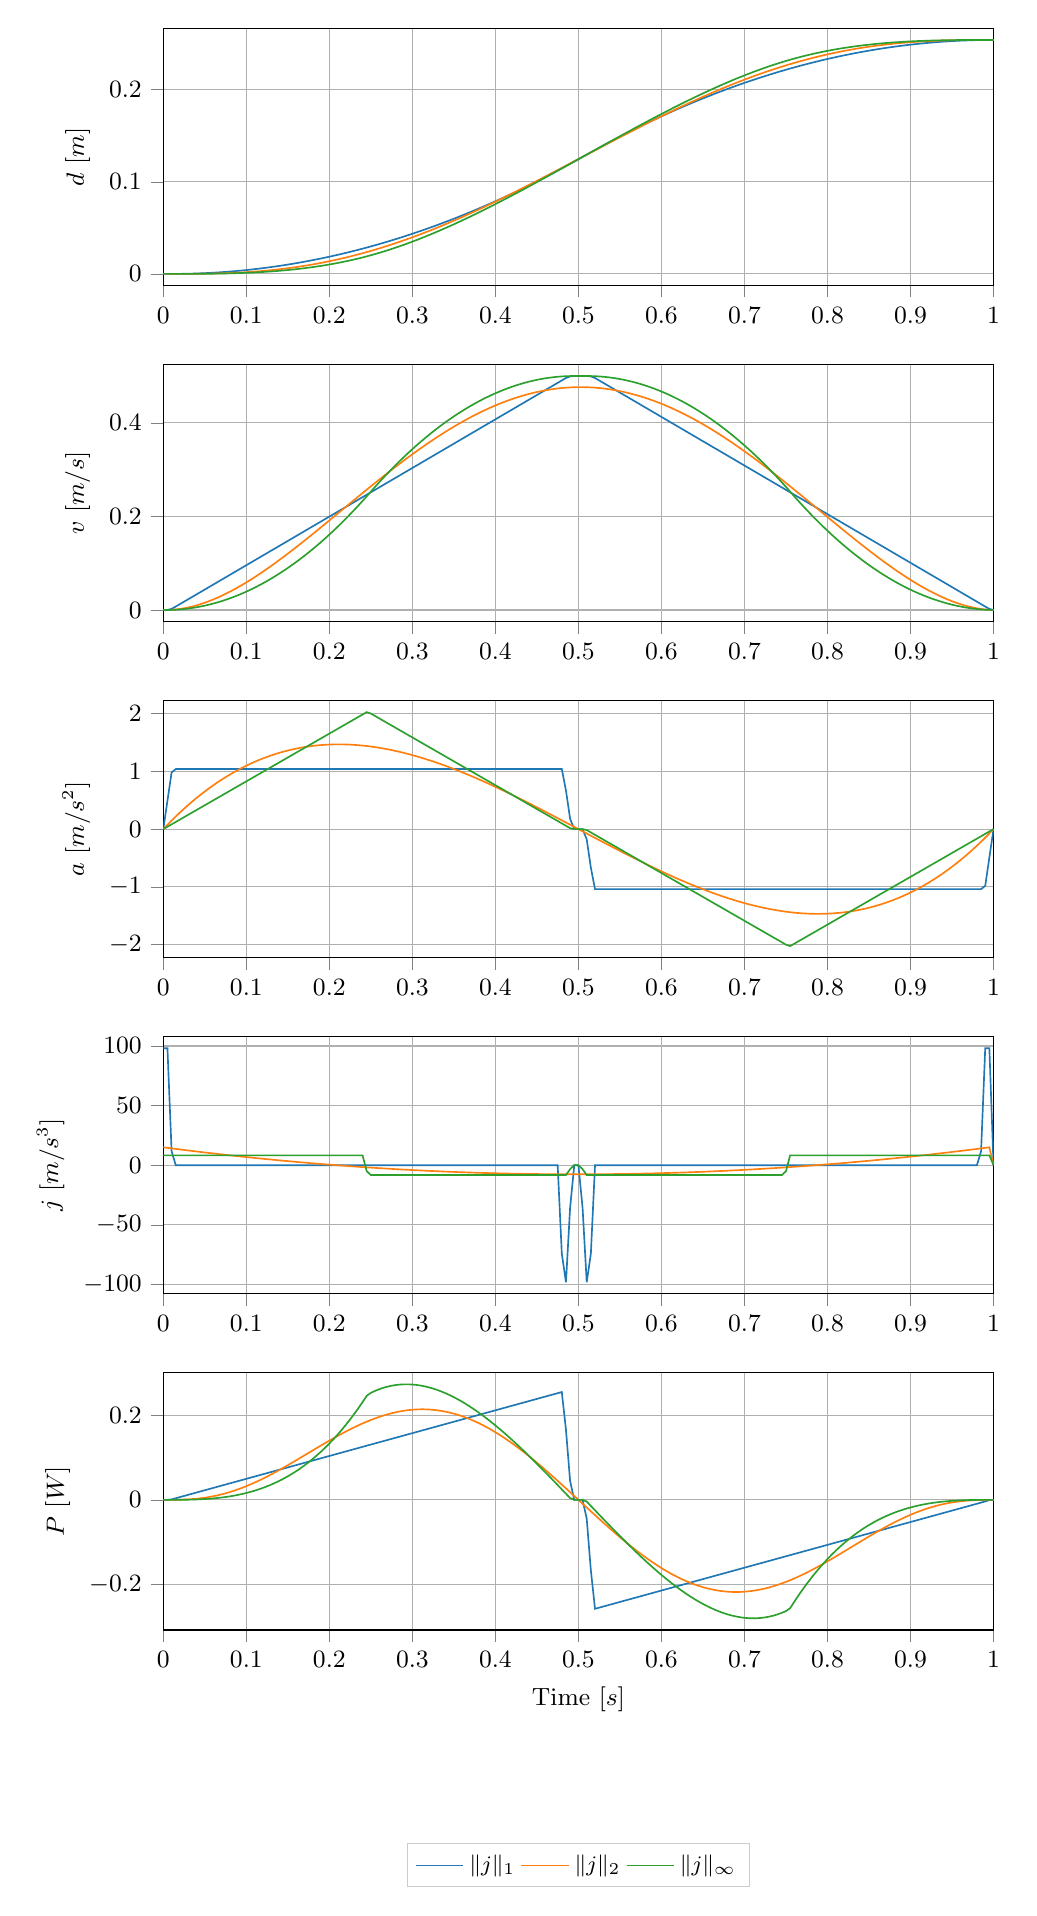
\begin{tikzpicture}

\definecolor{color0}{rgb}{0.12156862745098,0.466666666666667,0.705882352941177}
\definecolor{color1}{rgb}{1,0.498039215686275,0.0549019607843137}
\definecolor{color2}{rgb}{0.172549019607843,0.627450980392157,0.172549019607843}

\begin{groupplot}[group style={group size=1 by 5}]
\nextgroupplot[
tick align=outside,
tick pos=left,
x grid style={white!69.01960784313725!black},
xmajorgrids,
xmin=0, xmax=1,
y grid style={white!69.01960784313725!black},
%ylabel={Distance [$m$]},
ylabel={$d$ [$m$]},
ymajorgrids,
ymin=-0.0127, ymax=0.2667
%title = \footnotesize{Jerk}
]
\addplot [semithick, color0]
table [row sep=\\]{%
0	0 \\
0.005	-2.33564889720827e-45 \\
0.01	2.22040997396793e-45 \\
0.015	1.22624999986642e-05 \\
0.02	4.90499999933082e-05 \\
0.025	0.000111816755307425 \\
0.03	0.000200562765943674 \\
0.035	0.000315288031903358 \\
0.04	0.000455992553187333 \\
0.045	0.000622676329796226 \\
0.05	0.000815339361730528 \\
0.055	0.00103398164899064 \\
0.06	0.00127860319157689 \\
0.065	0.00154920398948958 \\
0.07	0.00184578404272894 \\
0.075	0.00216834335129518 \\
0.08	0.0025168819151885 \\
0.085	0.00289139973440907 \\
0.09	0.00329189680895702 \\
0.095	0.00371837313883249 \\
0.1	0.00417082872403559 \\
0.105	0.00464926356456643 \\
0.11	0.00515367766042509 \\
0.115	0.00568407101161166 \\
0.12	0.00624044361812621 \\
0.125	0.00682279547996879 \\
0.13	0.00743112659713945 \\
0.135	0.00806543696963824 \\
0.14	0.00872572659746519 \\
0.145	0.00941199548062034 \\
0.15	0.0101242436191037 \\
0.155	0.0108624710129153 \\
0.16	0.0116266776620551 \\
0.165	0.0124168635665231 \\
0.17	0.0132330287263193 \\
0.175	0.0140751731414438 \\
0.18	0.0149432968118964 \\
0.185	0.0158373997376772 \\
0.19	0.0167574819187861 \\
0.195	0.0177035433552231 \\
0.2	0.0186755840469881 \\
0.205	0.0196736039940811 \\
0.21	0.020697603196502 \\
0.215	0.0217475816542508 \\
0.22	0.0228235393673273 \\
0.225	0.0239254763357315 \\
0.23	0.0250533925594633 \\
0.235	0.0262072880385226 \\
0.24	0.0273871627729093 \\
0.245	0.0285930167626232 \\
0.25	0.0298248500076643 \\
0.255	0.0310826625080324 \\
0.26	0.0323664542637274 \\
0.265	0.033676225274749 \\
0.27	0.0350119755410972 \\
0.275	0.0363737050627718 \\
0.28	0.0377614138397725 \\
0.285	0.0391751018720992 \\
0.29	0.0406147691597516 \\
0.295	0.0420804157027295 \\
0.3	0.0435720415010326 \\
0.305	0.0450896465546608 \\
0.31	0.0466332308636136 \\
0.315	0.0482027944278908 \\
0.32	0.0497983372474921 \\
0.325	0.0514198593224171 \\
0.33	0.0530673606526654 \\
0.335	0.0547408412382366 \\
0.34	0.0564403010791303 \\
0.345	0.0581657401753461 \\
0.35	0.0599171585268833 \\
0.355	0.0616945561337415 \\
0.36	0.06349793299592 \\
0.365	0.0653272891134183 \\
0.37	0.0671826244862356 \\
0.375	0.0690639391143712 \\
0.38	0.0709712329978243 \\
0.385	0.0729045061365938 \\
0.39	0.0748637585306789 \\
0.395	0.0768489901800785 \\
0.4	0.0788602010847912 \\
0.405	0.0808973912448158 \\
0.41	0.0829605606601507 \\
0.415	0.0850497093307942 \\
0.42	0.0871648372567444 \\
0.425	0.089305944437999 \\
0.43	0.0914730308745555 \\
0.435	0.0936660965664109 \\
0.44	0.0958851415135618 \\
0.445	0.0981301657160038 \\
0.45	0.100401169173732 \\
0.455	0.10269815188674 \\
0.46	0.10502111385502 \\
0.465	0.107370055078562 \\
0.47	0.10974497555735 \\
0.475	0.112145875291365 \\
0.48	0.114572754280572 \\
0.485	0.117025612524909 \\
0.49	0.119504450024204 \\
0.495	0.122000000023402 \\
0.5	0.124500000023016 \\
0.505	0.12700000002283 \\
0.51	0.129500000022645 \\
0.515	0.132000000022259 \\
0.52	0.134495550020981 \\
0.525	0.136974387519325 \\
0.53	0.13942724576272 \\
0.535	0.141854124750997 \\
0.54	0.144255024484091 \\
0.545	0.146629944961968 \\
0.55	0.148978886184609 \\
0.555	0.151301848151999 \\
0.56	0.153598830864126 \\
0.565	0.155869834320984 \\
0.57	0.158114858522566 \\
0.575	0.160333903468867 \\
0.58	0.162526969159882 \\
0.585	0.164694055595609 \\
0.59	0.166835162776044 \\
0.595	0.168950290701184 \\
0.6	0.171039439371029 \\
0.605	0.173102608785574 \\
0.61	0.175139798944819 \\
0.615	0.177151009848763 \\
0.62	0.179136241497404 \\
0.625	0.18109549389074 \\
0.63	0.183028767028771 \\
0.635	0.184936060911495 \\
0.64	0.186817375538912 \\
0.645	0.188672710911021 \\
0.65	0.190502067027821 \\
0.655	0.192305443889312 \\
0.66	0.194082841495492 \\
0.665	0.195834259846361 \\
0.67	0.197559698941919 \\
0.675	0.199259158782165 \\
0.68	0.200932639367099 \\
0.685	0.20258014069672 \\
0.69	0.204201662771027 \\
0.695	0.205797205590021 \\
0.7	0.207366769153701 \\
0.705	0.208910353462067 \\
0.71	0.210427958515119 \\
0.715	0.211919584312855 \\
0.72	0.213385230855276 \\
0.725	0.214824898142382 \\
0.73	0.216238586174173 \\
0.735	0.217626294950647 \\
0.74	0.218988024471806 \\
0.745	0.220323774737648 \\
0.75	0.221633545748174 \\
0.755	0.222917337503383 \\
0.76	0.224175150003275 \\
0.765	0.225406983247851 \\
0.77	0.226612837237109 \\
0.775	0.227792711971051 \\
0.78	0.228946607449675 \\
0.785	0.230074523672982 \\
0.79	0.231176460640971 \\
0.795	0.232252418353643 \\
0.8	0.233302396810997 \\
0.805	0.234326396013033 \\
0.81	0.235324415959752 \\
0.815	0.236296456651152 \\
0.82	0.237242518087235 \\
0.825	0.238162600268 \\
0.83	0.239056703193447 \\
0.835	0.239924826863576 \\
0.84	0.240766971278386 \\
0.845	0.241583136437879 \\
0.85	0.242373322342054 \\
0.855	0.24313752899091 \\
0.86	0.243875756384448 \\
0.865	0.244588004522669 \\
0.87	0.245274273405571 \\
0.875	0.245934563033155 \\
0.88	0.246568873405421 \\
0.885	0.247177204522369 \\
0.89	0.247759556383999 \\
0.895	0.248315928990311 \\
0.9	0.248846322341305 \\
0.905	0.249350736436982 \\
0.91	0.249829171277341 \\
0.915	0.250281626862382 \\
0.92	0.250708103192106 \\
0.925	0.251108600266512 \\
0.93	0.251483118085601 \\
0.935	0.251831656649373 \\
0.94	0.252154215957828 \\
0.945	0.252450796010966 \\
0.95	0.252721396808787 \\
0.955	0.252966018351293 \\
0.96	0.253184660638482 \\
0.965	0.253377323670356 \\
0.97	0.253544007446914 \\
0.975	0.253684711968157 \\
0.98	0.253799437234087 \\
0.985	0.253888183244703 \\
0.99	0.253950950000007 \\
0.995	0.253987737500001 \\
1	0.254 \\
};
\addplot [semithick, color1]
table [row sep=\\]{%
0	0 \\
0.005	0 \\
0.01	-3.1861838222649e-58 \\
0.015	1.87675483974273e-06 \\
0.02	7.45043378590008e-06 \\
0.025	1.84851921035247e-05 \\
0.03	3.66897426274972e-05 \\
0.035	6.37179273339723e-05 \\
0.04	0.000101169288911824 \\
0.045	0.000150589642334092 \\
0.05	0.000213471646429427 \\
0.055	0.000291255375453534 \\
0.06	0.00038532889066062 \\
0.065	0.000497028811874838 \\
0.07	0.000627640889061733 \\
0.075	0.000778400573899687 \\
0.08	0.000950493591351361 \\
0.085	0.00114505651123515 \\
0.09	0.0013631773197966 \\
0.095	0.00160589599127991 \\
0.1	0.00187420505949931 \\
0.105	0.00216905018941056 \\
0.11	0.00249133074868235 \\
0.115	0.00284190037926778 \\
0.12	0.00322156756897579 \\
0.125	0.00363109622304261 \\
0.13	0.00407120623570322 \\
0.135	0.00454257406176273 \\
0.14	0.00504583328816793 \\
0.145	0.00558157520557864 \\
0.15	0.0061503493799392 \\
0.155	0.00675266422404993 \\
0.16	0.00738898756913852 \\
0.165	0.00805974723643154 \\
0.17	0.00876533160872583 \\
0.175	0.00950609020195999 \\
0.18	0.0102823342367858 \\
0.185	0.0110943372101396 \\
0.19	0.0119423354668139 \\
0.195	0.0128265287710288 \\
0.2	0.0137470808780031 \\
0.205	0.0147041201055262 \\
0.21	0.0156977399055294 \\
0.215	0.0167279994356572 \\
0.22	0.0177949241308388 \\
0.225	0.0188985062748597 \\
0.23	0.020038705571933 \\
0.235	0.0212154497182709 \\
0.24	0.0224286349736561 \\
0.245	0.0236781267330131 \\
0.25	0.0249637600979802 \\
0.255	0.0262853404484803 \\
0.26	0.0276426440142925 \\
0.265	0.0290354184466239 \\
0.27	0.0304633833896808 \\
0.275	0.0319262310522398 \\
0.28	0.03342362677922 \\
0.285	0.0349552096232538 \\
0.29	0.0365205929162586 \\
0.295	0.0381193648410083 \\
0.3	0.0397510890027045 \\
0.305	0.0414153050005484 \\
0.31	0.0431115289993116 \\
0.315	0.0448392543009083 \\
0.32	0.0465979519159659 \\
0.325	0.0483870711353972 \\
0.33	0.0502060401019715 \\
0.335	0.052054266381886 \\
0.34	0.0539311375363373 \\
0.345	0.0558360216930931 \\
0.35	0.0577682681180631 \\
0.355	0.0597272077868711 \\
0.36	0.0617121539564257 \\
0.365	0.0637224027364924 \\
0.37	0.0657572336612649 \\
0.375	0.0678159102609363 \\
0.38	0.0698976806332706 \\
0.385	0.0720017780151744 \\
0.39	0.0741274213542681 \\
0.395	0.0762738158804574 \\
0.4	0.0784401536775048 \\
0.405	0.0806256142546011 \\
0.41	0.0828293651179365 \\
0.415	0.0850505623422727 \\
0.42	0.0872883511425135 \\
0.425	0.089541866445277 \\
0.43	0.0918102334604668 \\
0.435	0.094092568252843 \\
0.44	0.0963879783135943 \\
0.445	0.0986955631319092 \\
0.45	0.101014414766547 \\
0.455	0.103343618417411 \\
0.46	0.105682252997117 \\
0.465	0.108029391702567 \\
0.47	0.110384102586519 \\
0.475	0.112745449129162 \\
0.48	0.115112490809683 \\
0.485	0.11748428367784 \\
0.49	0.119859880925534 \\
0.495	0.122238333458382 \\
0.5	0.124618690467284 \\
0.505	0.127 \\
0.51	0.129381309532716 \\
0.515	0.131761666541618 \\
0.52	0.134140119074466 \\
0.525	0.13651571632216 \\
0.53	0.138887509190317 \\
0.535	0.141254550870838 \\
0.54	0.143615897413481 \\
0.545	0.145970608297433 \\
0.55	0.148317747002883 \\
0.555	0.150656381582589 \\
0.56	0.152985585233453 \\
0.565	0.155304436868091 \\
0.57	0.157612021686406 \\
0.575	0.159907431747157 \\
0.58	0.162189766539533 \\
0.585	0.164458133554723 \\
0.59	0.166711648857487 \\
0.595	0.168949437657727 \\
0.6	0.171170634882063 \\
0.605	0.173374385745399 \\
0.61	0.175559846322495 \\
0.615	0.177726184119543 \\
0.62	0.179872578645732 \\
0.625	0.181998221984826 \\
0.63	0.184102319366729 \\
0.635	0.186184089739064 \\
0.64	0.188242766338735 \\
0.645	0.190277597263508 \\
0.65	0.192287846043574 \\
0.655	0.194272792213129 \\
0.66	0.196231731881937 \\
0.665	0.198163978306907 \\
0.67	0.200068862463663 \\
0.675	0.201945733618114 \\
0.68	0.203793959898029 \\
0.685	0.205612928864603 \\
0.69	0.207402048084034 \\
0.695	0.209160745699092 \\
0.7	0.210888471000688 \\
0.705	0.212584694999452 \\
0.71	0.214248910997295 \\
0.715	0.215880635158992 \\
0.72	0.217479407083741 \\
0.725	0.219044790376746 \\
0.73	0.22057637322078 \\
0.735	0.22207376894776 \\
0.74	0.223536616610319 \\
0.745	0.224964581553376 \\
0.75	0.226357355985707 \\
0.755	0.22771465955152 \\
0.76	0.22903623990202 \\
0.765	0.230321873266987 \\
0.77	0.231571365026344 \\
0.775	0.232784550281729 \\
0.78	0.233961294428067 \\
0.785	0.23510149372514 \\
0.79	0.236205075869161 \\
0.795	0.237272000564343 \\
0.8	0.238302260094471 \\
0.805	0.239295879894474 \\
0.81	0.240252919121997 \\
0.815	0.241173471228971 \\
0.82	0.242057664533186 \\
0.825	0.24290566278986 \\
0.83	0.243717665763214 \\
0.835	0.24449390979804 \\
0.84	0.245234668391274 \\
0.845	0.245940252763568 \\
0.85	0.246611012430861 \\
0.855	0.24724733577595 \\
0.86	0.247849650620061 \\
0.865	0.248418424794421 \\
0.87	0.248954166711832 \\
0.875	0.249457425938237 \\
0.88	0.249928793764297 \\
0.885	0.250368903776957 \\
0.89	0.250778432431024 \\
0.895	0.251158099620732 \\
0.9	0.251508669251318 \\
0.905	0.251830949810589 \\
0.91	0.252125794940501 \\
0.915	0.25239410400872 \\
0.92	0.252636822680203 \\
0.925	0.252854943488765 \\
0.93	0.253049506408649 \\
0.935	0.2532215994261 \\
0.94	0.253372359110938 \\
0.945	0.253502971188125 \\
0.95	0.253614671109339 \\
0.955	0.253708744624546 \\
0.96	0.253786528353571 \\
0.965	0.253849410357666 \\
0.97	0.253898830711088 \\
0.975	0.253936282072666 \\
0.98	0.253963310257373 \\
0.985	0.253981514807896 \\
0.99	0.253992549566214 \\
0.995	0.25399812324516 \\
1	0.254 \\
};
\addplot [semithick, color2]
table [row sep=\\]{%
0	0 \\
0.005	-4.93834723965812e-48 \\
0.01	4.12350114161078e-39 \\
0.015	1.03290299028283e-06 \\
0.02	4.13161196077499e-06 \\
0.025	1.03290299010289e-05 \\
0.03	2.06580598002041e-05 \\
0.035	3.61516046470467e-05 \\
0.04	5.78425674298679e-05 \\
0.045	8.67638511365204e-05 \\
0.05	0.000123948358754373 \\
0.055	0.000170428993270285 \\
0.06	0.000227238657670573 \\
0.065	0.000295410254940985 \\
0.07	0.000375976688066662 \\
0.075	0.0004699708600321 \\
0.08	0.000578425673821114 \\
0.085	0.000702374032416789 \\
0.09	0.000842848838801435 \\
0.095	0.00100088299595653 \\
0.1	0.00117750940686268 \\
0.105	0.00137376097449951 \\
0.11	0.00159067060184565 \\
0.115	0.00182927119187863 \\
0.12	0.00209059564757478 \\
0.125	0.00237567687190915 \\
0.13	0.00268554776785541 \\
0.135	0.0030212412383857 \\
0.14	0.00338379018647054 \\
0.145	0.0037742275150786 \\
0.15	0.00419358612717661 \\
0.155	0.00464289892572908 \\
0.16	0.00512319881369813 \\
0.165	0.00563551869404316 \\
0.17	0.00618089146972058 \\
0.175	0.00676035004368339 \\
0.18	0.00737492731888077 \\
0.185	0.00802565619825753 \\
0.19	0.00871356958475345 \\
0.195	0.00943970038130246 \\
0.2	0.0102050814908317 \\
0.205	0.01101074581626 \\
0.21	0.0118577262604967 \\
0.215	0.0127470557264389 \\
0.22	0.0136797671169684 \\
0.225	0.0146568933349478 \\
0.23	0.0156794672832134 \\
0.235	0.0167485218645646 \\
0.24	0.0178650899817458 \\
0.245	0.0190302045374087 \\
0.25	0.0202448984340201 \\
0.255	0.0215102045734902 \\
0.26	0.0228254982139116 \\
0.265	0.0241897464534195 \\
0.27	0.0256019163895927 \\
0.275	0.027060975119825 \\
0.28	0.028565889741418 \\
0.285	0.0301156273516179 \\
0.29	0.0317091550476347 \\
0.295	0.0333454399266523 \\
0.3	0.0350234490858354 \\
0.305	0.036742149622334 \\
0.31	0.0385005086332863 \\
0.315	0.0402974932158213 \\
0.32	0.0421320704670602 \\
0.325	0.0440032074841179 \\
0.33	0.0459098713641042 \\
0.335	0.0478510292041244 \\
0.34	0.0498256481012802 \\
0.345	0.0518326951526703 \\
0.35	0.0538711374553908 \\
0.355	0.0559399421065358 \\
0.36	0.0580380762031978 \\
0.365	0.0601645068424679 \\
0.37	0.0623182011214363 \\
0.375	0.0644981261371926 \\
0.38	0.0667032489868261 \\
0.385	0.0689325367674262 \\
0.39	0.0711849565760824 \\
0.395	0.073459475509885 \\
0.4	0.0757550606659251 \\
0.405	0.0780706791412951 \\
0.41	0.0804052980330892 \\
0.415	0.0827578844384034 \\
0.42	0.0851274054543365 \\
0.425	0.0875128281779901 \\
0.43	0.0899131197064696 \\
0.435	0.0923272471368847 \\
0.44	0.0947541775663504 \\
0.445	0.0971928780919879 \\
0.45	0.0996423158109261 \\
0.455	0.102101457820303 \\
0.46	0.104569271217269 \\
0.465	0.107044723098989 \\
0.47	0.109526780562647 \\
0.475	0.112014410705451 \\
0.48	0.11450658062465 \\
0.485	0.117002257417544 \\
0.49	0.119500408181527 \\
0.495	0.122000000014178 \\
0.5	0.124500000013633 \\
0.505	0.127 \\
0.51	0.129499999986367 \\
0.515	0.131999999985822 \\
0.52	0.134499591818473 \\
0.525	0.136997742582456 \\
0.53	0.13949341937535 \\
0.535	0.141985589294549 \\
0.54	0.144473219437353 \\
0.545	0.146955276901011 \\
0.55	0.149430728782731 \\
0.555	0.151898542179697 \\
0.56	0.154357684189074 \\
0.565	0.156807121908012 \\
0.57	0.15924582243365 \\
0.575	0.161672752863115 \\
0.58	0.16408688029353 \\
0.585	0.16648717182201 \\
0.59	0.168872594545664 \\
0.595	0.171242115561597 \\
0.6	0.173594701966911 \\
0.605	0.175929320858705 \\
0.61	0.178244939334075 \\
0.615	0.180540524490115 \\
0.62	0.182815043423918 \\
0.625	0.185067463232574 \\
0.63	0.187296751013174 \\
0.635	0.189501873862807 \\
0.64	0.191681798878564 \\
0.645	0.193835493157532 \\
0.65	0.195961923796802 \\
0.655	0.198060057893464 \\
0.66	0.200128862544609 \\
0.665	0.20216730484733 \\
0.67	0.20417435189872 \\
0.675	0.206148970795876 \\
0.68	0.208090128635896 \\
0.685	0.209996792515882 \\
0.69	0.21186792953294 \\
0.695	0.213702506784179 \\
0.7	0.215499491366714 \\
0.705	0.217257850377666 \\
0.71	0.218976550914165 \\
0.715	0.220654560073348 \\
0.72	0.222290844952365 \\
0.725	0.223884372648382 \\
0.73	0.225434110258582 \\
0.735	0.226939024880175 \\
0.74	0.228398083610407 \\
0.745	0.22981025354658 \\
0.75	0.231174501786088 \\
0.755	0.23248979542651 \\
0.76	0.23375510156598 \\
0.765	0.234969795462591 \\
0.77	0.236134910018254 \\
0.775	0.237251478135435 \\
0.78	0.238320532716787 \\
0.785	0.239343106665052 \\
0.79	0.240320232883032 \\
0.795	0.241252944273561 \\
0.8	0.242142273739503 \\
0.805	0.24298925418374 \\
0.81	0.243794918509168 \\
0.815	0.244560299618698 \\
0.82	0.245286430415247 \\
0.825	0.245974343801742 \\
0.83	0.246625072681119 \\
0.835	0.247239649956317 \\
0.84	0.247819108530279 \\
0.845	0.248364481305957 \\
0.85	0.248876801186302 \\
0.855	0.249357101074271 \\
0.86	0.249806413872823 \\
0.865	0.250225772484921 \\
0.87	0.250616209813529 \\
0.875	0.250978758761614 \\
0.88	0.251314452232145 \\
0.885	0.251624323128091 \\
0.89	0.251909404352425 \\
0.895	0.252170728808121 \\
0.9	0.252409329398154 \\
0.905	0.252626239025501 \\
0.91	0.252822490593137 \\
0.915	0.252999117004043 \\
0.92	0.253157151161199 \\
0.925	0.253297625967583 \\
0.93	0.253421574326179 \\
0.935	0.253530029139968 \\
0.94	0.253624023311933 \\
0.945	0.253704589745059 \\
0.95	0.253772761342329 \\
0.955	0.25382957100673 \\
0.96	0.253876051641246 \\
0.965	0.253913236148863 \\
0.97	0.25394215743257 \\
0.975	0.253963848395353 \\
0.98	0.2539793419402 \\
0.985	0.253989670970099 \\
0.99	0.253995868388039 \\
0.995	0.25399896709701 \\
1	0.254 \\
};
\nextgroupplot[
tick align=outside,
tick pos=left,
x grid style={white!69.01960784313725!black},
xmajorgrids,
xmin=0, xmax=1,
y grid style={white!69.01960784313725!black},
%ylabel={Velocity [$m/s$]},
ylabel={$v$ [$m/s$]},
ymajorgrids,
ymin=-0.0249999999981434, ymax=0.524999999961011
]
\addplot [semithick, color0, forget plot]
table [row sep=\\]{%
0	0 \\
0.005	2.37804044225857e-43 \\
0.01	0.00245249999973284 \\
0.015	0.0073574999989288 \\
0.02	0.0125533510628235 \\
0.025	0.0177492021272496 \\
0.03	0.0229450531919369 \\
0.035	0.028140904256795 \\
0.04	0.0333367553217786 \\
0.045	0.0385326063868605 \\
0.05	0.0437284574520223 \\
0.055	0.0489243085172511 \\
0.06	0.0541201595825367 \\
0.065	0.0593160106478715 \\
0.07	0.0645118617132491 \\
0.075	0.0697077127786643 \\
0.08	0.0749035638441126 \\
0.085	0.0800994149095903 \\
0.09	0.0852952659750939 \\
0.095	0.0904911170406207 \\
0.1	0.0956869681061678 \\
0.105	0.100882819171733 \\
0.11	0.106078670237314 \\
0.115	0.111274521302909 \\
0.12	0.116470372368516 \\
0.125	0.121666223434133 \\
0.13	0.126862074499758 \\
0.135	0.132057925565391 \\
0.14	0.137253776631028 \\
0.145	0.14244962769667 \\
0.15	0.147645478762314 \\
0.155	0.15284132982796 \\
0.16	0.158037180893605 \\
0.165	0.163233031959249 \\
0.17	0.16842888302489 \\
0.175	0.173624734090526 \\
0.18	0.178820585156157 \\
0.185	0.184016436221781 \\
0.19	0.189212287287397 \\
0.195	0.194408138353003 \\
0.2	0.199603989418599 \\
0.205	0.204799840484182 \\
0.21	0.209995691549751 \\
0.215	0.215191542615305 \\
0.22	0.220387393680842 \\
0.225	0.225583244746361 \\
0.23	0.23077909581186 \\
0.235	0.235974946877337 \\
0.24	0.24117079794279 \\
0.245	0.246366649008219 \\
0.25	0.25156250007362 \\
0.255	0.256758351138992 \\
0.26	0.261954202204332 \\
0.265	0.267150053269639 \\
0.27	0.27234590433491 \\
0.275	0.277541755400143 \\
0.28	0.282737606465334 \\
0.285	0.287933457530481 \\
0.29	0.293129308595581 \\
0.295	0.298325159660631 \\
0.3	0.303521010725628 \\
0.305	0.308716861790567 \\
0.31	0.313912712855444 \\
0.315	0.319108563920255 \\
0.32	0.324304414984996 \\
0.325	0.329500266049661 \\
0.33	0.334696117114246 \\
0.335	0.339891968178742 \\
0.34	0.345087819243145 \\
0.345	0.350283670307446 \\
0.35	0.355479521371639 \\
0.355	0.360675372435712 \\
0.36	0.365871223499658 \\
0.365	0.371067074563464 \\
0.37	0.376262925627118 \\
0.375	0.381458776690606 \\
0.38	0.386654627753913 \\
0.385	0.391850478817019 \\
0.39	0.397046329879906 \\
0.395	0.402242180942547 \\
0.4	0.407438032004917 \\
0.405	0.412633883066981 \\
0.41	0.417829734128703 \\
0.415	0.423025585190036 \\
0.42	0.428221436250925 \\
0.425	0.433417287311302 \\
0.43	0.438613138371084 \\
0.435	0.443808989430165 \\
0.44	0.449004840488411 \\
0.445	0.454200691545642 \\
0.45	0.459396542601618 \\
0.455	0.464592393655999 \\
0.46	0.469788244708288 \\
0.465	0.47498409575771 \\
0.47	0.480179946802948 \\
0.475	0.485375797841471 \\
0.48	0.490571648867308 \\
0.485	0.495767499858972 \\
0.49	0.499109999839636 \\
0.495	0.499999999922846 \\
0.5	0.499999999962867 \\
0.505	0.499999999962867 \\
0.51	0.499999999922846 \\
0.515	0.49910999974451 \\
0.52	0.495767499668719 \\
0.525	0.490571648679079 \\
0.53	0.485375797655267 \\
0.535	0.480179946618767 \\
0.54	0.474984095575553 \\
0.545	0.469788244528155 \\
0.55	0.46459239347789 \\
0.555	0.459396542425533 \\
0.56	0.454200691371581 \\
0.565	0.449004840316374 \\
0.57	0.443808989260152 \\
0.575	0.438613138203095 \\
0.58	0.433417287145336 \\
0.585	0.428221436086983 \\
0.59	0.423025585028118 \\
0.595	0.41782973396881 \\
0.6	0.412633882909112 \\
0.605	0.407438031849071 \\
0.61	0.402242180788726 \\
0.615	0.397046329728108 \\
0.62	0.391850478667246 \\
0.625	0.386654627606163 \\
0.63	0.381458776544881 \\
0.635	0.376262925483416 \\
0.64	0.371067074421786 \\
0.645	0.365871223360004 \\
0.65	0.360675372298083 \\
0.655	0.355479521236033 \\
0.66	0.350283670173865 \\
0.665	0.345087819111587 \\
0.67	0.339891968049208 \\
0.675	0.334696116986736 \\
0.68	0.329500265924176 \\
0.685	0.324304414861534 \\
0.69	0.319108563798817 \\
0.695	0.31391271273603 \\
0.7	0.308716861673176 \\
0.705	0.303521010610262 \\
0.71	0.298325159547289 \\
0.715	0.293129308484263 \\
0.72	0.287933457421187 \\
0.725	0.282737606358064 \\
0.73	0.277541755294896 \\
0.735	0.272345904231688 \\
0.74	0.267150053168441 \\
0.745	0.261954202105158 \\
0.75	0.256758351041841 \\
0.755	0.251562499978493 \\
0.76	0.246366648915116 \\
0.765	0.241170797851712 \\
0.77	0.235974946788282 \\
0.775	0.230779095724829 \\
0.78	0.225583244661354 \\
0.785	0.220387393597859 \\
0.79	0.215191542534346 \\
0.795	0.209995691470816 \\
0.8	0.204799840407271 \\
0.805	0.199603989343712 \\
0.81	0.194408138280141 \\
0.815	0.189212287216558 \\
0.82	0.184016436152966 \\
0.825	0.178820585089366 \\
0.83	0.173624734025759 \\
0.835	0.168428882962147 \\
0.84	0.16323303189853 \\
0.845	0.15803718083491 \\
0.85	0.152841329771289 \\
0.855	0.147645478707667 \\
0.86	0.142449627644047 \\
0.865	0.137253776580429 \\
0.87	0.132057925516815 \\
0.875	0.126862074453207 \\
0.88	0.121666223389605 \\
0.885	0.116470372326012 \\
0.89	0.11127452126243 \\
0.895	0.106078670198859 \\
0.9	0.100882819135302 \\
0.905	0.0956869680717604 \\
0.91	0.0904911170082372 \\
0.915	0.0852952659447344 \\
0.92	0.0800994148812547 \\
0.925	0.074903563817801 \\
0.93	0.0697077127543767 \\
0.935	0.0645118616909855 \\
0.94	0.0593160106276319 \\
0.945	0.054120159564321 \\
0.95	0.0489243085010593 \\
0.955	0.0437284574378546 \\
0.96	0.0385326063747167 \\
0.965	0.0333367553116587 \\
0.97	0.0281409042486991 \\
0.975	0.022945053185865 \\
0.98	0.0177492021232017 \\
0.985	0.0125533510607995 \\
0.99	0.0073574999989288 \\
0.995	0.00245249999973284 \\
1	0 \\
};
\addplot [semithick, color1, forget plot]
table [row sep=\\]{%
0	0 \\
0.005	0 \\
0.01	0.000375350967948546 \\
0.015	0.00111473578923147 \\
0.02	0.00220695166352493 \\
0.025	0.0036409101047945 \\
0.03	0.00540563694129501 \\
0.035	0.00749027231557038 \\
0.04	0.00988407068445365 \\
0.045	0.0125764008190669 \\
0.05	0.0155567458048214 \\
0.055	0.0188147030414172 \\
0.06	0.0223399842428437 \\
0.065	0.026122415437379 \\
0.07	0.0301519369675906 \\
0.075	0.0344186034903348 \\
0.08	0.038912583976757 \\
0.085	0.0436241617122915 \\
0.09	0.0485437342966619 \\
0.095	0.0536618136438805 \\
0.1	0.0589690259822488 \\
0.105	0.0644561118543574 \\
0.11	0.0701139261170858 \\
0.115	0.0759334379416026 \\
0.12	0.0819057308133652 \\
0.125	0.0880220025321203 \\
0.13	0.0942735652119035 \\
0.135	0.100651845281039 \\
0.14	0.107148383482142 \\
0.145	0.113754834872113 \\
0.15	0.120462968822145 \\
0.155	0.127264669017719 \\
0.16	0.134151933458604 \\
0.165	0.141116874458858 \\
0.17	0.148151718646831 \\
0.175	0.155248806965157 \\
0.18	0.162400594670765 \\
0.185	0.169599651334867 \\
0.19	0.176838660842968 \\
0.195	0.184110421394861 \\
0.2	0.191407845504628 \\
0.205	0.198723960000639 \\
0.21	0.206051906025555 \\
0.215	0.213384939036324 \\
0.22	0.220716428804184 \\
0.225	0.228039859414663 \\
0.23	0.235348829267576 \\
0.235	0.242637051077029 \\
0.24	0.249898351871415 \\
0.245	0.257126672993417 \\
0.25	0.264316070100007 \\
0.255	0.271460713162447 \\
0.26	0.278554886466287 \\
0.265	0.285592988611365 \\
0.27	0.29256953251181 \\
0.275	0.299479145396039 \\
0.28	0.306316568806758 \\
0.285	0.313076658600962 \\
0.29	0.319754384949935 \\
0.295	0.326344832339251 \\
0.3	0.332843199568772 \\
0.305	0.339244799752649 \\
0.31	0.345545060319323 \\
0.315	0.351739523011522 \\
0.32	0.357823843886264 \\
0.325	0.363793793314858 \\
0.33	0.3696452559829 \\
0.335	0.375374230890274 \\
0.34	0.380976831351155 \\
0.345	0.386449284994007 \\
0.35	0.391787933761581 \\
0.355	0.39698923391092 \\
0.36	0.402049756013354 \\
0.365	0.406966184954501 \\
0.37	0.411735319934271 \\
0.375	0.416354074466861 \\
0.38	0.420819476380758 \\
0.385	0.425128667818736 \\
0.39	0.429278905237861 \\
0.395	0.433267559409485 \\
0.4	0.437092115419252 \\
0.405	0.440750172667093 \\
0.41	0.444239444867228 \\
0.415	0.447557760048168 \\
0.42	0.450703060552709 \\
0.425	0.453673403037941 \\
0.43	0.45646695847524 \\
0.435	0.459082012150271 \\
0.44	0.461516963662988 \\
0.445	0.463770326927637 \\
0.45	0.465840730172748 \\
0.455	0.467726915941143 \\
0.46	0.469427741089934 \\
0.465	0.470942176790519 \\
0.47	0.472269308528588 \\
0.475	0.473408336104116 \\
0.48	0.474358573631372 \\
0.485	0.475119449538911 \\
0.49	0.475690506569576 \\
0.495	0.4760714017805 \\
0.5	0.476261906543107 \\
0.505	0.476261906543107 \\
0.51	0.4760714017805 \\
0.515	0.475690506569576 \\
0.52	0.475119449538911 \\
0.525	0.474358573631372 \\
0.53	0.473408336104116 \\
0.535	0.472269308528588 \\
0.54	0.470942176790519 \\
0.545	0.469427741089934 \\
0.55	0.467726915941143 \\
0.555	0.465840730172748 \\
0.56	0.463770326927637 \\
0.565	0.461516963662988 \\
0.57	0.459082012150271 \\
0.575	0.45646695847524 \\
0.58	0.453673403037941 \\
0.585	0.450703060552709 \\
0.59	0.447557760048168 \\
0.595	0.444239444867228 \\
0.6	0.440750172667093 \\
0.605	0.437092115419252 \\
0.61	0.433267559409485 \\
0.615	0.429278905237861 \\
0.62	0.425128667818736 \\
0.625	0.420819476380758 \\
0.63	0.416354074466861 \\
0.635	0.411735319934271 \\
0.64	0.406966184954501 \\
0.645	0.402049756013354 \\
0.65	0.39698923391092 \\
0.655	0.391787933761581 \\
0.66	0.386449284994007 \\
0.665	0.380976831351155 \\
0.67	0.375374230890274 \\
0.675	0.3696452559829 \\
0.68	0.363793793314858 \\
0.685	0.357823843886264 \\
0.69	0.351739523011522 \\
0.695	0.345545060319323 \\
0.7	0.339244799752649 \\
0.705	0.332843199568772 \\
0.71	0.326344832339251 \\
0.715	0.319754384949935 \\
0.72	0.313076658600962 \\
0.725	0.306316568806758 \\
0.73	0.299479145396039 \\
0.735	0.29256953251181 \\
0.74	0.285592988611365 \\
0.745	0.278554886466287 \\
0.75	0.271460713162447 \\
0.755	0.264316070100007 \\
0.76	0.257126672993417 \\
0.765	0.249898351871415 \\
0.77	0.242637051077029 \\
0.775	0.235348829267576 \\
0.78	0.228039859414663 \\
0.785	0.220716428804184 \\
0.79	0.213384939036324 \\
0.795	0.206051906025555 \\
0.8	0.198723960000639 \\
0.805	0.191407845504628 \\
0.81	0.184110421394861 \\
0.815	0.176838660842968 \\
0.82	0.169599651334867 \\
0.825	0.162400594670765 \\
0.83	0.155248806965157 \\
0.835	0.148151718646831 \\
0.84	0.141116874458858 \\
0.845	0.134151933458604 \\
0.85	0.127264669017719 \\
0.855	0.120462968822145 \\
0.86	0.113754834872113 \\
0.865	0.107148383482142 \\
0.87	0.100651845281039 \\
0.875	0.0942735652119035 \\
0.88	0.0880220025321203 \\
0.885	0.0819057308133652 \\
0.89	0.0759334379416026 \\
0.895	0.0701139261170858 \\
0.9	0.0644561118543574 \\
0.905	0.0589690259822488 \\
0.91	0.0536618136438805 \\
0.915	0.0485437342966619 \\
0.92	0.0436241617122915 \\
0.925	0.038912583976757 \\
0.93	0.0344186034903348 \\
0.935	0.0301519369675906 \\
0.94	0.026122415437379 \\
0.945	0.0223399842428437 \\
0.95	0.0188147030414172 \\
0.955	0.0155567458048214 \\
0.96	0.0125764008190669 \\
0.965	0.00988407068445365 \\
0.97	0.00749027231557038 \\
0.975	0.00540563694129501 \\
0.98	0.0036409101047945 \\
0.985	0.00220695166352493 \\
0.99	0.00111473578923147 \\
0.995	0.000375350967948546 \\
1	0 \\
};
\addplot [semithick, color2, forget plot]
table [row sep=\\]{%
0	0 \\
0.005	6.46398974360891e-46 \\
0.01	0.000206580598056566 \\
0.015	0.000619741794098431 \\
0.02	0.00123948358805079 \\
0.025	0.00206580597983504 \\
0.03	0.00309870896936853 \\
0.035	0.00433819255656424 \\
0.04	0.00578425674133049 \\
0.045	0.00743690152357056 \\
0.05	0.00929612690318229 \\
0.055	0.0113619328800577 \\
0.06	0.0136343194540824 \\
0.065	0.0161132866251353 \\
0.07	0.0187988343930876 \\
0.075	0.0216909627578027 \\
0.08	0.024789671719135 \\
0.085	0.0280949612769292 \\
0.09	0.0316068314310196 \\
0.095	0.0353252821812288 \\
0.1	0.0392503135273666 \\
0.105	0.0433819254692288 \\
0.11	0.0477201180065955 \\
0.115	0.0522648911392295 \\
0.12	0.0570162448668743 \\
0.125	0.0619741791892516 \\
0.13	0.067138694106059 \\
0.135	0.0725097896169664 \\
0.14	0.0780874657216128 \\
0.145	0.0838717224196015 \\
0.15	0.0898625597104952 \\
0.155	0.0960599775938098 \\
0.16	0.102463976069007 \\
0.165	0.109074555135483 \\
0.17	0.115891714792562 \\
0.175	0.122915455039477 \\
0.18	0.130145775875352 \\
0.185	0.137582677299183 \\
0.19	0.145226159309802 \\
0.195	0.153076221905842 \\
0.2	0.161132865085675 \\
0.205	0.16939608884734 \\
0.21	0.177865893188426 \\
0.215	0.186542278105909 \\
0.22	0.19542524359588 \\
0.225	0.204514789653108 \\
0.23	0.213810916270245 \\
0.235	0.223313623436232 \\
0.24	0.233022911132589 \\
0.245	0.242938779322278 \\
0.25	0.253061227894024 \\
0.255	0.263058728084283 \\
0.26	0.272849647901577 \\
0.265	0.282433987234642 \\
0.27	0.291811746046463 \\
0.275	0.300982924318584 \\
0.28	0.309947522039984 \\
0.285	0.318705539203356 \\
0.29	0.327256975803519 \\
0.295	0.335601831836626 \\
0.3	0.34374010729972 \\
0.305	0.351671802190468 \\
0.31	0.359396916506996 \\
0.315	0.366915450247775 \\
0.32	0.374227403411544 \\
0.325	0.381332775997256 \\
0.33	0.388231568004039 \\
0.335	0.394923779431162 \\
0.34	0.401409410278018 \\
0.345	0.407688460544102 \\
0.35	0.413760930229005 \\
0.355	0.419626819332394 \\
0.36	0.425286127854015 \\
0.365	0.43073885579368 \\
0.37	0.435985003151265 \\
0.375	0.441024569926711 \\
0.38	0.445857556120016 \\
0.385	0.450483961731243 \\
0.39	0.454903786760514 \\
0.395	0.459117031208015 \\
0.4	0.463123695074004 \\
0.405	0.466923778358811 \\
0.41	0.470517281062847 \\
0.415	0.473904203186615 \\
0.42	0.477084544730723 \\
0.425	0.480058305695902 \\
0.43	0.482825486083024 \\
0.435	0.485386085893137 \\
0.44	0.4877401051275 \\
0.445	0.489887543787643 \\
0.45	0.491828401875441 \\
0.455	0.493562679393224 \\
0.46	0.495090376343952 \\
0.465	0.496411492731472 \\
0.47	0.497526028560963 \\
0.475	0.498433983839731 \\
0.48	0.499135358578802 \\
0.485	0.499630152796627 \\
0.49	0.499918366530225 \\
0.495	0.499999999890863 \\
0.5	0.499999997273479 \\
0.505	0.499999997273479 \\
0.51	0.499999999890863 \\
0.515	0.499918366530225 \\
0.52	0.499630152796627 \\
0.525	0.499135358578802 \\
0.53	0.498433983839731 \\
0.535	0.497526028560963 \\
0.54	0.496411492731472 \\
0.545	0.495090376343952 \\
0.55	0.493562679393224 \\
0.555	0.491828401875441 \\
0.56	0.489887543787643 \\
0.565	0.4877401051275 \\
0.57	0.485386085893137 \\
0.575	0.482825486083024 \\
0.58	0.480058305695902 \\
0.585	0.477084544730723 \\
0.59	0.473904203186615 \\
0.595	0.470517281062847 \\
0.6	0.466923778358811 \\
0.605	0.463123695074004 \\
0.61	0.459117031208015 \\
0.615	0.454903786760514 \\
0.62	0.450483961731243 \\
0.625	0.445857556120016 \\
0.63	0.441024569926711 \\
0.635	0.435985003151265 \\
0.64	0.43073885579368 \\
0.645	0.425286127854015 \\
0.65	0.419626819332394 \\
0.655	0.413760930229005 \\
0.66	0.407688460544102 \\
0.665	0.401409410278018 \\
0.67	0.394923779431162 \\
0.675	0.388231568004039 \\
0.68	0.381332775997256 \\
0.685	0.374227403411544 \\
0.69	0.366915450247775 \\
0.695	0.359396916506996 \\
0.7	0.351671802190468 \\
0.705	0.34374010729972 \\
0.71	0.335601831836626 \\
0.715	0.327256975803519 \\
0.72	0.318705539203356 \\
0.725	0.309947522039984 \\
0.73	0.300982924318584 \\
0.735	0.291811746046463 \\
0.74	0.282433987234642 \\
0.745	0.272849647901577 \\
0.75	0.263058728084283 \\
0.755	0.253061227894024 \\
0.76	0.242938779322278 \\
0.765	0.233022911132589 \\
0.77	0.223313623436232 \\
0.775	0.213810916270245 \\
0.78	0.204514789653108 \\
0.785	0.19542524359588 \\
0.79	0.186542278105909 \\
0.795	0.177865893188426 \\
0.8	0.16939608884734 \\
0.805	0.161132865085675 \\
0.81	0.153076221905842 \\
0.815	0.145226159309802 \\
0.82	0.137582677299183 \\
0.825	0.130145775875352 \\
0.83	0.122915455039477 \\
0.835	0.115891714792562 \\
0.84	0.109074555135483 \\
0.845	0.102463976069007 \\
0.85	0.0960599775938098 \\
0.855	0.0898625597104952 \\
0.86	0.0838717224196015 \\
0.865	0.0780874657216128 \\
0.87	0.0725097896169664 \\
0.875	0.067138694106059 \\
0.88	0.0619741791892516 \\
0.885	0.0570162448668743 \\
0.89	0.0522648911392295 \\
0.895	0.0477201180065955 \\
0.9	0.0433819254692288 \\
0.905	0.0392503135273666 \\
0.91	0.0353252821812288 \\
0.915	0.0316068314310196 \\
0.92	0.0280949612769292 \\
0.925	0.024789671719135 \\
0.93	0.0216909627578027 \\
0.935	0.0187988343930876 \\
0.94	0.0161132866251353 \\
0.945	0.0136343194540824 \\
0.95	0.0113619328800577 \\
0.955	0.00929612690318229 \\
0.96	0.00743690152357056 \\
0.965	0.00578425674133049 \\
0.97	0.00433819255656424 \\
0.975	0.00309870896936853 \\
0.98	0.00206580597983504 \\
0.985	0.00123948358805079 \\
0.99	0.000619741794098431 \\
0.995	0.000206580598056566 \\
1	0 \\
};
\nextgroupplot[
tick align=outside,
tick pos=left,
x grid style={white!69.01960784313725!black},
xmajorgrids,
xmin=0, xmax=1,
y grid style={white!69.01960784313725!black},
%ylabel={Acceleration [$m/s^2$]},
ylabel={$a$ [$m/s^2$]},
ymajorgrids,
ymin=-2.226938685784, ymax=2.226938685784
]
\addplot [semithick, color0, forget plot]
table [row sep=\\]{%
0	0 \\
0.005	0.490499999946568 \\
0.01	0.980999999839191 \\
0.015	1.03917021277893 \\
0.02	1.03917021288523 \\
0.025	1.03917021293745 \\
0.03	1.03917021297161 \\
0.035	1.03917021299672 \\
0.04	1.03917021301638 \\
0.045	1.03917021303238 \\
0.05	1.03917021304575 \\
0.055	1.03917021305713 \\
0.06	1.03917021306696 \\
0.065	1.03917021307552 \\
0.07	1.03917021308303 \\
0.075	1.03917021308966 \\
0.08	1.03917021309553 \\
0.085	1.03917021310073 \\
0.09	1.03917021310535 \\
0.095	1.03917021310943 \\
0.1	1.03917021311304 \\
0.105	1.03917021311621 \\
0.11	1.03917021311897 \\
0.115	1.03917021312136 \\
0.12	1.0391702131234 \\
0.125	1.0391702131251 \\
0.13	1.03917021312648 \\
0.135	1.03917021312757 \\
0.14	1.03917021312836 \\
0.145	1.03917021312886 \\
0.15	1.03917021312909 \\
0.155	1.03917021312904 \\
0.16	1.03917021312873 \\
0.165	1.03917021312815 \\
0.17	1.03917021312731 \\
0.175	1.0391702131262 \\
0.18	1.03917021312482 \\
0.185	1.03917021312318 \\
0.19	1.03917021312126 \\
0.195	1.03917021311907 \\
0.2	1.0391702131166 \\
0.205	1.03917021311384 \\
0.21	1.03917021311079 \\
0.215	1.03917021310743 \\
0.22	1.03917021310376 \\
0.225	1.03917021309976 \\
0.23	1.03917021309542 \\
0.235	1.03917021309073 \\
0.24	1.03917021308567 \\
0.245	1.03917021308023 \\
0.25	1.03917021307438 \\
0.255	1.03917021306811 \\
0.26	1.03917021306138 \\
0.265	1.03917021305419 \\
0.27	1.03917021304649 \\
0.275	1.03917021303826 \\
0.28	1.03917021302946 \\
0.285	1.03917021302006 \\
0.29	1.03917021301 \\
0.295	1.03917021299926 \\
0.3	1.03917021298776 \\
0.305	1.03917021297546 \\
0.31	1.03917021296229 \\
0.315	1.03917021294818 \\
0.32	1.03917021293305 \\
0.325	1.03917021291681 \\
0.33	1.03917021289935 \\
0.335	1.03917021288055 \\
0.34	1.03917021286029 \\
0.345	1.03917021283841 \\
0.35	1.03917021281475 \\
0.355	1.03917021278909 \\
0.36	1.03917021276121 \\
0.365	1.03917021273084 \\
0.37	1.03917021269766 \\
0.375	1.03917021266131 \\
0.38	1.03917021262134 \\
0.385	1.03917021257722 \\
0.39	1.03917021252833 \\
0.395	1.03917021247389 \\
0.4	1.03917021241295 \\
0.405	1.03917021234433 \\
0.41	1.03917021226656 \\
0.415	1.03917021217775 \\
0.42	1.03917021207544 \\
0.425	1.03917021195641 \\
0.43	1.03917021181631 \\
0.435	1.03917021164911 \\
0.44	1.03917021144626 \\
0.445	1.03917021119512 \\
0.45	1.03917021087624 \\
0.455	1.03917021045788 \\
0.46	1.03917020988436 \\
0.465	1.03917020904757 \\
0.47	1.03917020770467 \\
0.475	1.03917020516739 \\
0.48	1.03917019833268 \\
0.485	0.668499996132869 \\
0.49	0.178000016641908 \\
0.495	8.00432223520196e-09 \\
0.5	-1.58887947641678e-15 \\
0.505	-8.00431740738352e-09 \\
0.51	-0.178000035667193 \\
0.515	-0.668500015158154 \\
0.52	-1.03917019792789 \\
0.525	-1.03917020476259 \\
0.53	-1.03917020729987 \\
0.535	-1.03917020864277 \\
0.54	-1.03917020947957 \\
0.545	-1.03917021005309 \\
0.55	-1.03917021047145 \\
0.555	-1.03917021079033 \\
0.56	-1.03917021104147 \\
0.565	-1.03917021124432 \\
0.57	-1.03917021141152 \\
0.575	-1.03917021155162 \\
0.58	-1.03917021167065 \\
0.585	-1.03917021177295 \\
0.59	-1.03917021186177 \\
0.595	-1.03917021193954 \\
0.6	-1.03917021200815 \\
0.605	-1.03917021206909 \\
0.61	-1.03917021212354 \\
0.615	-1.03917021217243 \\
0.62	-1.03917021221654 \\
0.625	-1.03917021225651 \\
0.63	-1.03917021229287 \\
0.635	-1.03917021232604 \\
0.64	-1.03917021235641 \\
0.645	-1.03917021238429 \\
0.65	-1.03917021240995 \\
0.655	-1.03917021243362 \\
0.66	-1.0391702124555 \\
0.665	-1.03917021247576 \\
0.67	-1.03917021249455 \\
0.675	-1.03917021251201 \\
0.68	-1.03917021252826 \\
0.685	-1.03917021254339 \\
0.69	-1.0391702125575 \\
0.695	-1.03917021257067 \\
0.7	-1.03917021258297 \\
0.705	-1.03917021259446 \\
0.71	-1.03917021260521 \\
0.715	-1.03917021261526 \\
0.72	-1.03917021262467 \\
0.725	-1.03917021263347 \\
0.73	-1.0391702126417 \\
0.735	-1.0391702126494 \\
0.74	-1.03917021265659 \\
0.745	-1.03917021266331 \\
0.75	-1.03917021266959 \\
0.755	-1.03917021267543 \\
0.76	-1.03917021268088 \\
0.765	-1.03917021268593 \\
0.77	-1.03917021269062 \\
0.775	-1.03917021269496 \\
0.78	-1.03917021269896 \\
0.785	-1.03917021270264 \\
0.79	-1.039170212706 \\
0.795	-1.03917021270905 \\
0.8	-1.03917021271181 \\
0.805	-1.03917021271428 \\
0.81	-1.03917021271647 \\
0.815	-1.03917021271839 \\
0.82	-1.03917021272003 \\
0.825	-1.0391702127214 \\
0.83	-1.03917021272251 \\
0.835	-1.03917021272336 \\
0.84	-1.03917021272394 \\
0.845	-1.03917021272425 \\
0.85	-1.03917021272429 \\
0.855	-1.03917021272407 \\
0.86	-1.03917021272356 \\
0.865	-1.03917021272277 \\
0.87	-1.03917021272169 \\
0.875	-1.03917021272031 \\
0.88	-1.0391702127186 \\
0.885	-1.03917021271657 \\
0.89	-1.03917021271418 \\
0.895	-1.03917021271141 \\
0.9	-1.03917021270824 \\
0.905	-1.03917021270464 \\
0.91	-1.03917021270055 \\
0.915	-1.03917021269594 \\
0.92	-1.03917021269074 \\
0.925	-1.03917021268487 \\
0.93	-1.03917021267824 \\
0.935	-1.03917021267073 \\
0.94	-1.03917021266216 \\
0.945	-1.03917021265234 \\
0.95	-1.03917021264095 \\
0.955	-1.03917021262758 \\
0.96	-1.03917021261158 \\
0.965	-1.03917021259193 \\
0.97	-1.03917021256682 \\
0.975	-1.03917021253266 \\
0.98	-1.03917021248044 \\
0.985	-1.03917021237414 \\
0.99	-0.980999999839191 \\
0.995	-0.490499999946568 \\
1	0 \\
};
\addplot [semithick, color1, forget plot]
table [row sep=\\]{%
0	0 \\
0.005	0.0750701935897093 \\
0.01	0.147876964256585 \\
0.015	0.218443174858691 \\
0.02	0.286791688253915 \\
0.025	0.352945367300101 \\
0.03	0.416927074855074 \\
0.035	0.478759673776655 \\
0.04	0.538466026922656 \\
0.045	0.596068997150889 \\
0.05	0.651591447319165 \\
0.055	0.70505624028529 \\
0.06	0.756486238907074 \\
0.065	0.805904306042321 \\
0.07	0.853333304548839 \\
0.075	0.898796097284432 \\
0.08	0.942315547106907 \\
0.085	0.983914516874069 \\
0.09	1.02361586944372 \\
0.095	1.06144246767367 \\
0.1	1.09741717442172 \\
0.105	1.13156285254568 \\
0.11	1.16390236490334 \\
0.115	1.19445857435252 \\
0.12	1.22325434375102 \\
0.125	1.25031253595664 \\
0.13	1.27565601382719 \\
0.135	1.29930764022046 \\
0.14	1.32129027799427 \\
0.145	1.34162679000642 \\
0.15	1.36034003911471 \\
0.155	1.37745288817695 \\
0.16	1.39298820005094 \\
0.165	1.40696883759448 \\
0.17	1.41941766366537 \\
0.175	1.43035754112143 \\
0.18	1.43981133282045 \\
0.185	1.44780190162024 \\
0.19	1.4543521103786 \\
0.195	1.45948482195334 \\
0.2	1.46322289920225 \\
0.205	1.46558920498315 \\
0.21	1.46660660215383 \\
0.215	1.4662979535721 \\
0.22	1.46468612209577 \\
0.225	1.46179397058263 \\
0.23	1.45764436189049 \\
0.235	1.45226015887715 \\
0.24	1.44566422440042 \\
0.245	1.4378794213181 \\
0.25	1.428928612488 \\
0.255	1.41883466076791 \\
0.26	1.40762042901564 \\
0.265	1.39530878008899 \\
0.27	1.38192257684577 \\
0.275	1.36748468214378 \\
0.28	1.35201795884083 \\
0.285	1.33554526979471 \\
0.29	1.31808947786323 \\
0.295	1.29967344590419 \\
0.3	1.28032003677541 \\
0.305	1.26005211333467 \\
0.31	1.23889253843978 \\
0.315	1.21686417494855 \\
0.32	1.19398988571878 \\
0.325	1.17029253360827 \\
0.33	1.14579498147483 \\
0.335	1.12052009217625 \\
0.34	1.09449072857035 \\
0.345	1.06772975351492 \\
0.35	1.04026002986777 \\
0.355	1.0121044204867 \\
0.36	0.983285788229511 \\
0.365	0.953826995954011 \\
0.37	0.923750906518001 \\
0.375	0.893080382779282 \\
0.38	0.861838287595659 \\
0.385	0.830047483824933 \\
0.39	0.797730834324907 \\
0.395	0.764911201953384 \\
0.4	0.731611449568166 \\
0.405	0.697854440027055 \\
0.41	0.663663036187854 \\
0.415	0.629060100908363 \\
0.42	0.594068497046385 \\
0.425	0.558711087459721 \\
0.43	0.523010735006172 \\
0.435	0.486990302543538 \\
0.44	0.450672652929618 \\
0.445	0.414080649022213 \\
0.45	0.377237153679119 \\
0.455	0.340165029758135 \\
0.46	0.302887140117055 \\
0.465	0.265426347613675 \\
0.47	0.227805515105787 \\
0.475	0.190047505451183 \\
0.48	0.152175181507653 \\
0.485	0.114211406132984 \\
0.49	0.076179042184962 \\
0.495	0.0381009525213728 \\
0.5	1.29732143385112e-17 \\
0.505	-0.0381009525213728 \\
0.51	-0.076179042184962 \\
0.515	-0.114211406132984 \\
0.52	-0.152175181507653 \\
0.525	-0.190047505451183 \\
0.53	-0.227805515105787 \\
0.535	-0.265426347613675 \\
0.54	-0.302887140117055 \\
0.545	-0.340165029758135 \\
0.55	-0.377237153679119 \\
0.555	-0.414080649022213 \\
0.56	-0.450672652929618 \\
0.565	-0.486990302543538 \\
0.57	-0.523010735006172 \\
0.575	-0.558711087459721 \\
0.58	-0.594068497046385 \\
0.585	-0.629060100908363 \\
0.59	-0.663663036187854 \\
0.595	-0.697854440027055 \\
0.6	-0.731611449568166 \\
0.605	-0.764911201953384 \\
0.61	-0.797730834324907 \\
0.615	-0.830047483824933 \\
0.62	-0.861838287595659 \\
0.625	-0.893080382779282 \\
0.63	-0.923750906518001 \\
0.635	-0.953826995954011 \\
0.64	-0.983285788229511 \\
0.645	-1.0121044204867 \\
0.65	-1.04026002986777 \\
0.655	-1.06772975351492 \\
0.66	-1.09449072857035 \\
0.665	-1.12052009217625 \\
0.67	-1.14579498147483 \\
0.675	-1.17029253360827 \\
0.68	-1.19398988571878 \\
0.685	-1.21686417494855 \\
0.69	-1.23889253843978 \\
0.695	-1.26005211333467 \\
0.7	-1.28032003677541 \\
0.705	-1.29967344590419 \\
0.71	-1.31808947786323 \\
0.715	-1.33554526979471 \\
0.72	-1.35201795884083 \\
0.725	-1.36748468214378 \\
0.73	-1.38192257684577 \\
0.735	-1.39530878008899 \\
0.74	-1.40762042901564 \\
0.745	-1.41883466076791 \\
0.75	-1.428928612488 \\
0.755	-1.4378794213181 \\
0.76	-1.44566422440042 \\
0.765	-1.45226015887715 \\
0.77	-1.45764436189049 \\
0.775	-1.46179397058263 \\
0.78	-1.46468612209577 \\
0.785	-1.4662979535721 \\
0.79	-1.46660660215383 \\
0.795	-1.46558920498315 \\
0.8	-1.46322289920225 \\
0.805	-1.45948482195334 \\
0.81	-1.4543521103786 \\
0.815	-1.44780190162024 \\
0.82	-1.43981133282045 \\
0.825	-1.43035754112143 \\
0.83	-1.41941766366537 \\
0.835	-1.40696883759448 \\
0.84	-1.39298820005094 \\
0.845	-1.37745288817695 \\
0.85	-1.36034003911471 \\
0.855	-1.34162679000642 \\
0.86	-1.32129027799427 \\
0.865	-1.29930764022046 \\
0.87	-1.27565601382719 \\
0.875	-1.25031253595664 \\
0.88	-1.22325434375102 \\
0.885	-1.19445857435252 \\
0.89	-1.16390236490334 \\
0.895	-1.13156285254568 \\
0.9	-1.09741717442172 \\
0.905	-1.06144246767367 \\
0.91	-1.02361586944372 \\
0.915	-0.983914516874069 \\
0.92	-0.942315547106907 \\
0.925	-0.898796097284432 \\
0.93	-0.853333304548839 \\
0.935	-0.805904306042321 \\
0.94	-0.756486238907074 \\
0.945	-0.70505624028529 \\
0.95	-0.651591447319165 \\
0.955	-0.596068997150889 \\
0.96	-0.538466026922656 \\
0.965	-0.478759673776655 \\
0.97	-0.416927074855074 \\
0.975	-0.352945367300101 \\
0.98	-0.286791688253915 \\
0.985	-0.218443174858691 \\
0.99	-0.147876964256585 \\
0.995	-0.0750701935897093 \\
1	0 \\
};
\addplot [semithick, color2, forget plot]
table [row sep=\\]{%
0	0 \\
0.005	0.0413161196113132 \\
0.01	0.0826322392083731 \\
0.015	0.123948358790471 \\
0.02	0.16526447835685 \\
0.025	0.206580597906697 \\
0.03	0.247896717439143 \\
0.035	0.28921283695325 \\
0.04	0.330528956448014 \\
0.045	0.371845075922347 \\
0.05	0.41316119537508 \\
0.055	0.454477314804946 \\
0.06	0.495793434210573 \\
0.065	0.537109553590471 \\
0.07	0.57842567294302 \\
0.075	0.619741792266454 \\
0.08	0.661057911558844 \\
0.085	0.702374030818078 \\
0.09	0.743690150041835 \\
0.095	0.785006269227562 \\
0.1	0.826322388372438 \\
0.105	0.867638507473342 \\
0.11	0.908954626526804 \\
0.115	0.950270745528956 \\
0.12	0.991586864475467 \\
0.125	1.03290298336147 \\
0.13	1.07421910218148 \\
0.135	1.11553522092927 \\
0.14	1.15685133959774 \\
0.145	1.19816745817875 \\
0.15	1.23948357666292 \\
0.155	1.28079969503936 \\
0.16	1.32211581329533 \\
0.165	1.3634319314158 \\
0.17	1.40474804938288 \\
0.175	1.44606416717506 \\
0.18	1.48738028476617 \\
0.185	1.52869640212393 \\
0.19	1.57001251920792 \\
0.195	1.61132863596662 \\
0.2	1.65264475233294 \\
0.205	1.69396086821733 \\
0.21	1.7352769834965 \\
0.215	1.77659309799418 \\
0.22	1.81790921144571 \\
0.225	1.85922532342739 \\
0.23	1.90054143319736 \\
0.235	1.94185753927136 \\
0.24	1.98317363793785 \\
0.245	2.02448971434909 \\
0.25	1.99950003805196 \\
0.255	1.95818396345869 \\
0.26	1.9168678666131 \\
0.265	1.87555176236402 \\
0.27	1.83423565442438 \\
0.275	1.79291954427999 \\
0.28	1.75160343267429 \\
0.285	1.71028732003267 \\
0.29	1.66897120662145 \\
0.295	1.62765509261872 \\
0.3	1.58633897814959 \\
0.305	1.54502286330557 \\
0.31	1.50370674815576 \\
0.315	1.46239063275384 \\
0.32	1.42107451714252 \\
0.325	1.37975840135652 \\
0.33	1.33844228542461 \\
0.335	1.29712616937112 \\
0.34	1.25581005321695 \\
0.345	1.21449393698044 \\
0.35	1.1731778206779 \\
0.355	1.13186170432416 \\
0.36	1.09054558793292 \\
0.365	1.04922947151711 \\
0.37	1.00791335508913 \\
0.375	0.966597238661145 \\
0.38	0.92528112224533 \\
0.385	0.883965005854094 \\
0.39	0.842648889500354 \\
0.395	0.801332773197815 \\
0.4	0.7600166569613 \\
0.405	0.718700540807135 \\
0.41	0.677384424753639 \\
0.415	0.636068308821729 \\
0.42	0.594752193035723 \\
0.425	0.553436077424405 \\
0.43	0.512119962022487 \\
0.435	0.470803846872672 \\
0.44	0.42948773202864 \\
0.445	0.388171617559506 \\
0.45	0.346855503556763 \\
0.455	0.305539390145541 \\
0.46	0.264223277503898 \\
0.465	0.222907165898187 \\
0.47	0.181591055753766 \\
0.475	0.140274947814102 \\
0.48	0.0989588435650225 \\
0.485	0.0576427467196186 \\
0.49	0.0163266721276458 \\
0.495	-5.23476821390392e-07 \\
0.5	5.07563702478095e-23 \\
0.505	5.23476821390392e-07 \\
0.51	-0.0163266721276458 \\
0.515	-0.0576427467196186 \\
0.52	-0.0989588435650225 \\
0.525	-0.140274947814102 \\
0.53	-0.181591055753766 \\
0.535	-0.222907165898187 \\
0.54	-0.264223277503898 \\
0.545	-0.305539390145541 \\
0.55	-0.346855503556763 \\
0.555	-0.388171617559506 \\
0.56	-0.42948773202864 \\
0.565	-0.470803846872672 \\
0.57	-0.512119962022487 \\
0.575	-0.553436077424405 \\
0.58	-0.594752193035723 \\
0.585	-0.636068308821729 \\
0.59	-0.677384424753639 \\
0.595	-0.718700540807135 \\
0.6	-0.7600166569613 \\
0.605	-0.801332773197815 \\
0.61	-0.842648889500354 \\
0.615	-0.883965005854094 \\
0.62	-0.92528112224533 \\
0.625	-0.966597238661145 \\
0.63	-1.00791335508913 \\
0.635	-1.04922947151711 \\
0.64	-1.09054558793292 \\
0.645	-1.13186170432416 \\
0.65	-1.1731778206779 \\
0.655	-1.21449393698044 \\
0.66	-1.25581005321695 \\
0.665	-1.29712616937112 \\
0.67	-1.33844228542461 \\
0.675	-1.37975840135652 \\
0.68	-1.42107451714252 \\
0.685	-1.46239063275384 \\
0.69	-1.50370674815576 \\
0.695	-1.54502286330557 \\
0.7	-1.58633897814959 \\
0.705	-1.62765509261872 \\
0.71	-1.66897120662145 \\
0.715	-1.71028732003267 \\
0.72	-1.75160343267429 \\
0.725	-1.79291954427999 \\
0.73	-1.83423565442438 \\
0.735	-1.87555176236402 \\
0.74	-1.9168678666131 \\
0.745	-1.95818396345869 \\
0.75	-1.99950003805196 \\
0.755	-2.02448971434909 \\
0.76	-1.98317363793785 \\
0.765	-1.94185753927136 \\
0.77	-1.90054143319736 \\
0.775	-1.85922532342739 \\
0.78	-1.81790921144571 \\
0.785	-1.77659309799418 \\
0.79	-1.7352769834965 \\
0.795	-1.69396086821733 \\
0.8	-1.65264475233294 \\
0.805	-1.61132863596662 \\
0.81	-1.57001251920792 \\
0.815	-1.52869640212393 \\
0.82	-1.48738028476617 \\
0.825	-1.44606416717506 \\
0.83	-1.40474804938288 \\
0.835	-1.3634319314158 \\
0.84	-1.32211581329533 \\
0.845	-1.28079969503936 \\
0.85	-1.23948357666292 \\
0.855	-1.19816745817875 \\
0.86	-1.15685133959774 \\
0.865	-1.11553522092927 \\
0.87	-1.07421910218148 \\
0.875	-1.03290298336147 \\
0.88	-0.991586864475467 \\
0.885	-0.950270745528956 \\
0.89	-0.908954626526804 \\
0.895	-0.867638507473342 \\
0.9	-0.826322388372438 \\
0.905	-0.785006269227562 \\
0.91	-0.743690150041835 \\
0.915	-0.702374030818078 \\
0.92	-0.661057911558844 \\
0.925	-0.619741792266454 \\
0.93	-0.57842567294302 \\
0.935	-0.537109553590471 \\
0.94	-0.495793434210573 \\
0.945	-0.454477314804946 \\
0.95	-0.41316119537508 \\
0.955	-0.371845075922347 \\
0.96	-0.330528956448014 \\
0.965	-0.28921283695325 \\
0.97	-0.247896717439143 \\
0.975	-0.206580597906697 \\
0.98	-0.16526447835685 \\
0.985	-0.123948358790471 \\
0.99	-0.0826322392083731 \\
0.995	-0.0413161196113132 \\
1	0 \\
};
\nextgroupplot[
tick align=outside,
tick pos=left,
x grid style={white!69.01960784313725!black},
xmajorgrids,
xmin=0, xmax=1,
y grid style={white!69.01960784313725!black},
%ylabel={Jerk [$m/s^3$]},
ylabel={$j$ [$m/s^3$]},
ymajorgrids,
ymin=-107.909995692568, ymax=107.909999783689
]
\addplot [semithick, color0, forget plot]
table [row sep=\\]{%
0	98.0999999893137 \\
0.005	98.0999999785245 \\
0.01	11.6340425879481 \\
0.015	2.12603534384257e-08 \\
0.02	1.04438291483777e-08 \\
0.025	6.83241037550169e-09 \\
0.03	5.02166870669885e-09 \\
0.035	3.93090296964917e-09 \\
0.04	3.19990801659138e-09 \\
0.045	2.67431145428926e-09 \\
0.05	2.27692168711333e-09 \\
0.055	1.9648471625704e-09 \\
0.06	1.71234500618346e-09 \\
0.065	1.50302524903898e-09 \\
0.07	1.32595303510317e-09 \\
0.075	1.17354982418028e-09 \\
0.08	1.04039406006921e-09 \\
0.085	9.22501536007482e-10 \\
0.09	8.16875578752172e-10 \\
0.095	7.21215941128867e-10 \\
0.1	6.33724675880023e-10 \\
0.105	5.52973254031454e-10 \\
0.11	4.77809485427708e-10 \\
0.115	4.07290966991134e-10 \\
0.12	3.40636610689307e-10 \\
0.125	2.77190740796458e-10 \\
0.13	2.16396085932777e-10 \\
0.135	1.57773166170041e-10 \\
0.14	1.00904343490235e-10 \\
0.145	4.5421315699175e-11 \\
0.15	-9.00481898382003e-12 \\
0.155	-6.26715602685298e-11 \\
0.16	-1.15851533495365e-10 \\
0.165	-1.68797894756092e-10 \\
0.17	-2.21748876732046e-10 \\
0.175	-2.74931677259595e-10 \\
0.18	-3.28565847982894e-10 \\
0.185	-3.82866307756901e-10 \\
0.19	-4.38046081493554e-10 \\
0.195	-4.94318847635267e-10 \\
0.2	-5.51901364825225e-10 \\
0.205	-6.11015839505954e-10 \\
0.21	-6.71892290337642e-10 \\
0.215	-7.34770961976588e-10 \\
0.22	-7.99904839527153e-10 \\
0.225	-8.67562315694345e-10 \\
0.23	-9.38030065223636e-10 \\
0.235	-1.01161618566649e-09 \\
0.24	-1.08865366994838e-09 \\
0.245	-1.16950428490277e-09 \\
0.25	-1.25456294117491e-09 \\
0.255	-1.34426265424183e-09 \\
0.26	-1.4390802142008e-09 \\
0.265	-1.53954270460894e-09 \\
0.27	-1.64623503860111e-09 \\
0.275	-1.75980871590598e-09 \\
0.28	-1.88099204818502e-09 \\
0.285	-2.01060215571268e-09 \\
0.29	-2.1495591081482e-09 \\
0.295	-2.29890267107848e-09 \\
0.3	-2.45981223264341e-09 \\
0.305	-2.63363062999092e-09 \\
0.31	-2.82189278190628e-09 \\
0.315	-3.02636027706493e-09 \\
0.32	-3.24906338454504e-09 \\
0.325	-3.49235237167069e-09 \\
0.33	-3.75896056924305e-09 \\
0.335	-4.05208236736583e-09 \\
0.34	-4.37547032834499e-09 \\
0.345	-4.733556971293e-09 \\
0.35	-5.131608666201e-09 \\
0.355	-5.57592169646247e-09 \\
0.36	-6.0740742386147e-09 \\
0.365	-6.63525326676789e-09 \\
0.37	-7.27068298420069e-09 \\
0.375	-7.99419251159675e-09 \\
0.38	-8.82297712004283e-09 \\
0.385	-9.77863235699632e-09 \\
0.39	-1.08885790512725e-08 \\
0.395	-1.2188057975512e-08 \\
0.4	-1.37229707656497e-08 \\
0.405	-1.55540050679831e-08 \\
0.41	-1.77627555858213e-08 \\
0.415	-2.04610316473727e-08 \\
0.42	-2.38054101542816e-08 \\
0.425	-2.80207314396943e-08 \\
0.43	-3.34394750498213e-08 \\
0.435	-4.05707110506901e-08 \\
0.44	-5.02273440036296e-08 \\
0.445	-6.37763654515031e-08 \\
0.45	-8.36713411499204e-08 \\
0.455	-1.1470423516555e-07 \\
0.46	-1.673590940949e-07 \\
0.465	-2.68580199037433e-07 \\
0.47	-5.07455795276752e-07 \\
0.475	-1.36694070820603e-06 \\
0.48	-74.1340404399629 \\
0.485	-98.0999958981922 \\
0.49	-35.6000017275172 \\
0.495	-1.60086476481633e-06 \\
0.5	-1.60086316370076e-06 \\
0.505	-35.6000055325752 \\
0.51	-98.0999958981922 \\
0.515	-74.1340365539473 \\
0.52	-1.36694070821117e-06 \\
0.525	-5.07455794726167e-07 \\
0.53	-2.68580198546493e-07 \\
0.535	-1.67359093746167e-07 \\
0.54	-1.14704234936553e-07 \\
0.545	-8.36713409981254e-08 \\
0.55	-6.37763653508011e-08 \\
0.555	-5.02273439351385e-08 \\
0.56	-4.05707110032054e-08 \\
0.565	-3.34394750161399e-08 \\
0.57	-2.80207314153878e-08 \\
0.575	-2.38054101363702e-08 \\
0.58	-2.04610316338592e-08 \\
0.585	-1.77627555755214e-08 \\
0.59	-1.55540050599337e-08 \\
0.595	-1.372297075928e-08 \\
0.6	-1.21880579703773e-08 \\
0.605	-1.08885790470937e-08 \\
0.61	-9.77863235353449e-09 \\
0.615	-8.82297711715445e-09 \\
0.62	-7.99419250915645e-09 \\
0.625	-7.27068298210979e-09 \\
0.63	-6.63525326497006e-09 \\
0.635	-6.07407423704514e-09 \\
0.64	-5.57592169509197e-09 \\
0.645	-5.13160866499101e-09 \\
0.65	-4.73355697021896e-09 \\
0.655	-4.37547032739123e-09 \\
0.66	-4.05208236651277e-09 \\
0.665	-3.75896056847543e-09 \\
0.67	-3.49235237097443e-09 \\
0.675	-3.24906338392035e-09 \\
0.68	-3.02636027649784e-09 \\
0.685	-2.82189278138387e-09 \\
0.69	-2.63363062950483e-09 \\
0.695	-2.45981223220116e-09 \\
0.7	-2.29890267067052e-09 \\
0.705	-2.14955910777233e-09 \\
0.71	-2.01060215536052e-09 \\
0.715	-1.88099204786886e-09 \\
0.72	-1.75980871561539e-09 \\
0.725	-1.64623503833377e-09 \\
0.73	-1.53954270435938e-09 \\
0.735	-1.43908021397009e-09 \\
0.74	-1.34426265402303e-09 \\
0.745	-1.25456294097212e-09 \\
0.75	-1.16950428471435e-09 \\
0.755	-1.08865366977553e-09 \\
0.76	-1.01161618550616e-09 \\
0.765	-9.38030065074346e-10 \\
0.77	-8.6756231555477e-10 \\
0.775	-7.9990483939667e-10 \\
0.78	-7.34770961854218e-10 \\
0.785	-6.71892290222379e-10 \\
0.79	-6.11015839397057e-10 \\
0.795	-5.51901364722059e-10 \\
0.8	-4.94318847537064e-10 \\
0.805	-4.38046081400043e-10 \\
0.81	-3.82866307667381e-10 \\
0.815	-3.28565847896914e-10 \\
0.82	-2.7493167717679e-10 \\
0.825	-2.21748876652101e-10 \\
0.83	-1.68797894678509e-10 \\
0.835	-1.15851533419622e-10 \\
0.84	-6.26715601945468e-11 \\
0.845	-9.00481891108107e-12 \\
0.85	4.54213157708552e-11 \\
0.855	1.00904343561253e-10 \\
0.86	1.57773166240768e-10 \\
0.865	2.16396086003451e-10 \\
0.87	2.77190740867503e-10 \\
0.875	3.40636610761146e-10 \\
0.88	4.07290967063979e-10 \\
0.885	4.77809485501823e-10 \\
0.89	5.52973254107793e-10 \\
0.895	6.33724675958797e-10 \\
0.9	7.21215941211506e-10 \\
0.905	8.16875578836663e-10 \\
0.91	9.22501536095997e-10 \\
0.915	1.04039406016302e-09 \\
0.92	1.17354982428065e-09 \\
0.925	1.3259530352099e-09 \\
0.93	1.50302524915577e-09 \\
0.935	1.71234500630946e-09 \\
0.94	1.96484716271143e-09 \\
0.945	2.27692168727109e-09 \\
0.95	2.67431145447095e-09 \\
0.955	3.19990801680441e-09 \\
0.96	3.93090296991048e-09 \\
0.965	5.0216687070347e-09 \\
0.97	6.83241037597688e-09 \\
0.975	1.04438291491765e-08 \\
0.98	2.12603534403332e-08 \\
0.985	11.6340425069894 \\
0.99	98.0999999785245 \\
0.995	98.0999999893137 \\
1	-1.08262427158294e-23 \\
};
\addplot [semithick, color1, forget plot]
table [row sep=\\]{%
0	15.0140387179419 \\
0.005	14.5613541333751 \\
0.01	14.1132421204213 \\
0.015	13.6697026790448 \\
0.02	13.2307358092371 \\
0.025	12.7963415109947 \\
0.03	12.3665197843161 \\
0.035	11.9412706292002 \\
0.04	11.5205940456467 \\
0.045	11.1044900336551 \\
0.05	10.6929585932251 \\
0.055	10.2859997243566 \\
0.06	9.88361342704946 \\
0.065	9.48579970130353 \\
0.07	9.09255854711873 \\
0.075	8.70388996449502 \\
0.08	8.31979395343235 \\
0.085	7.94027051393065 \\
0.09	7.56531964598991 \\
0.095	7.19494134961008 \\
0.1	6.82913562479115 \\
0.105	6.4679024715331 \\
0.11	6.11124188983589 \\
0.115	5.75915387969952 \\
0.12	5.41163844112398 \\
0.125	5.06869557410924 \\
0.13	4.7303252786553 \\
0.135	4.39652755476214 \\
0.14	4.06730240242977 \\
0.145	3.74264982165816 \\
0.15	3.42256981244731 \\
0.155	3.10706237479722 \\
0.16	2.79612750870787 \\
0.165	2.48976521417927 \\
0.17	2.1879754912114 \\
0.175	1.89075833980426 \\
0.18	1.59811375995785 \\
0.185	1.31004175167216 \\
0.19	1.02654231494719 \\
0.195	0.747615449782927 \\
0.2	0.473261156179376 \\
0.205	0.20347943413653 \\
0.21	-0.0617297163456139 \\
0.215	-0.32236629526706 \\
0.22	-0.578430302627811 \\
0.225	-0.82992173842787 \\
0.23	-1.07684060266724 \\
0.235	-1.31918689534593 \\
0.24	-1.55696061646393 \\
0.245	-1.79016176602126 \\
0.25	-2.01879034401791 \\
0.255	-2.24284635045388 \\
0.26	-2.46232978532919 \\
0.265	-2.67724064864383 \\
0.27	-2.8875789403978 \\
0.275	-3.09334466059112 \\
0.28	-3.29453780922378 \\
0.285	-3.49115838629578 \\
0.29	-3.68320639180713 \\
0.295	-3.87068182575784 \\
0.3	-4.0535846881479 \\
0.305	-4.23191497897732 \\
0.31	-4.40567269824611 \\
0.315	-4.57485784595426 \\
0.32	-4.73947042210179 \\
0.325	-4.89951042668869 \\
0.33	-5.05497785971497 \\
0.335	-5.20587272118064 \\
0.34	-5.3521950110857 \\
0.345	-5.49394472943016 \\
0.35	-5.63112187621402 \\
0.355	-5.7637264514373 \\
0.36	-5.89175845509999 \\
0.365	-6.01521788720212 \\
0.37	-6.13410474774368 \\
0.375	-6.2484190367247 \\
0.38	-6.35816075414518 \\
0.385	-6.46332990000514 \\
0.39	-6.56392647430462 \\
0.395	-6.65995047704361 \\
0.4	-6.75140190822217 \\
0.405	-6.83828076784032 \\
0.41	-6.9205870558981 \\
0.415	-6.99832077239557 \\
0.42	-7.0714819173328 \\
0.425	-7.14007049070985 \\
0.43	-7.20408649252684 \\
0.435	-7.26352992278388 \\
0.44	-7.31840078148112 \\
0.445	-7.36869906861873 \\
0.45	-7.41442478419691 \\
0.455	-7.45557792821591 \\
0.46	-7.49215850067602 \\
0.465	-7.52416650157752 \\
0.47	-7.55160193092077 \\
0.475	-7.57446478870609 \\
0.48	-7.59275507493385 \\
0.485	-7.60647278960435 \\
0.49	-7.61561793271785 \\
0.495	-7.62019050427455 \\
0.5	-7.62019050427455 \\
0.505	-7.61561793271785 \\
0.51	-7.60647278960435 \\
0.515	-7.59275507493385 \\
0.52	-7.57446478870609 \\
0.525	-7.55160193092077 \\
0.53	-7.52416650157752 \\
0.535	-7.49215850067602 \\
0.54	-7.45557792821591 \\
0.545	-7.41442478419691 \\
0.55	-7.36869906861873 \\
0.555	-7.31840078148112 \\
0.56	-7.26352992278388 \\
0.565	-7.20408649252684 \\
0.57	-7.14007049070986 \\
0.575	-7.0714819173328 \\
0.58	-6.99832077239557 \\
0.585	-6.9205870558981 \\
0.59	-6.83828076784032 \\
0.595	-6.75140190822217 \\
0.6	-6.65995047704361 \\
0.605	-6.56392647430461 \\
0.61	-6.46332990000514 \\
0.615	-6.35816075414518 \\
0.62	-6.2484190367247 \\
0.625	-6.13410474774368 \\
0.63	-6.01521788720212 \\
0.635	-5.89175845509999 \\
0.64	-5.7637264514373 \\
0.645	-5.63112187621402 \\
0.65	-5.49394472943016 \\
0.655	-5.3521950110857 \\
0.66	-5.20587272118064 \\
0.665	-5.05497785971497 \\
0.67	-4.89951042668869 \\
0.675	-4.73947042210179 \\
0.68	-4.57485784595426 \\
0.685	-4.40567269824611 \\
0.69	-4.23191497897732 \\
0.695	-4.0535846881479 \\
0.7	-3.87068182575784 \\
0.705	-3.68320639180713 \\
0.71	-3.49115838629578 \\
0.715	-3.29453780922378 \\
0.72	-3.09334466059112 \\
0.725	-2.8875789403978 \\
0.73	-2.67724064864383 \\
0.735	-2.46232978532919 \\
0.74	-2.24284635045388 \\
0.745	-2.01879034401791 \\
0.75	-1.79016176602126 \\
0.755	-1.55696061646393 \\
0.76	-1.31918689534593 \\
0.765	-1.07684060266724 \\
0.77	-0.829921738427871 \\
0.775	-0.578430302627811 \\
0.78	-0.32236629526706 \\
0.785	-0.0617297163456145 \\
0.79	0.203479434136529 \\
0.795	0.473261156179375 \\
0.8	0.747615449782926 \\
0.805	1.02654231494719 \\
0.81	1.31004175167216 \\
0.815	1.59811375995785 \\
0.82	1.89075833980426 \\
0.825	2.1879754912114 \\
0.83	2.48976521417927 \\
0.835	2.79612750870787 \\
0.84	3.10706237479722 \\
0.845	3.42256981244731 \\
0.85	3.74264982165816 \\
0.855	4.06730240242977 \\
0.86	4.39652755476214 \\
0.865	4.7303252786553 \\
0.87	5.06869557410924 \\
0.875	5.41163844112398 \\
0.88	5.75915387969953 \\
0.885	6.11124188983589 \\
0.89	6.4679024715331 \\
0.895	6.82913562479116 \\
0.9	7.19494134961008 \\
0.905	7.56531964598991 \\
0.91	7.94027051393065 \\
0.915	8.31979395343235 \\
0.92	8.70388996449503 \\
0.925	9.09255854711873 \\
0.93	9.48579970130353 \\
0.935	9.88361342704946 \\
0.94	10.2859997243566 \\
0.945	10.6929585932251 \\
0.95	11.1044900336551 \\
0.955	11.5205940456467 \\
0.96	11.9412706292002 \\
0.965	12.3665197843161 \\
0.97	12.7963415109947 \\
0.975	13.2307358092371 \\
0.98	13.6697026790448 \\
0.985	14.1132421204213 \\
0.99	14.5613541333751 \\
0.995	15.0140387179419 \\
1	0 \\
};
\addplot [semithick, color2, forget plot]
table [row sep=\\]{%
0	8.26322392226264 \\
0.005	8.26322391941197 \\
0.01	8.26322391641964 \\
0.015	8.26322391327575 \\
0.02	8.2632239099695 \\
0.025	8.26322390648907 \\
0.03	8.26322390282152 \\
0.035	8.26322389895262 \\
0.04	8.26322389486673 \\
0.045	8.2632238905466 \\
0.05	8.26322388597317 \\
0.055	8.26322388112531 \\
0.06	8.26322387597957 \\
0.065	8.26322387050982 \\
0.07	8.26322386468688 \\
0.075	8.26322385847809 \\
0.08	8.26322385184673 \\
0.085	8.26322384475141 \\
0.09	8.26322383714533 \\
0.095	8.26322382897533 \\
0.1	8.26322382018081 \\
0.105	8.26322381069239 \\
0.11	8.26322380043027 \\
0.115	8.26322378930226 \\
0.12	8.26322377720121 \\
0.125	8.26322376400194 \\
0.13	8.26322374955731 \\
0.135	8.26322373369319 \\
0.14	8.26322371620202 \\
0.145	8.26322369683442 \\
0.15	8.26322367528823 \\
0.155	8.26322365119372 \\
0.16	8.26322362409375 \\
0.165	8.26322359341645 \\
0.17	8.26322355843684 \\
0.175	8.26322351822218 \\
0.18	8.263223471552 \\
0.185	8.26322341679808 \\
0.19	8.26322335173912 \\
0.195	8.26322327326405 \\
0.2	8.26322317687759 \\
0.205	8.26322305583499 \\
0.21	8.26322289953508 \\
0.215	8.26322269030635 \\
0.22	8.26322239633611 \\
0.225	8.2632219539937 \\
0.23	8.26322121480027 \\
0.235	8.26321973329747 \\
0.24	8.26321528224787 \\
0.245	-4.99793525942475 \\
0.25	-8.26321491865396 \\
0.255	-8.26321936911831 \\
0.26	-8.2632208498163 \\
0.265	-8.26322158792777 \\
0.27	-8.26322202887921 \\
0.275	-8.26322232113835 \\
0.28	-8.26322252832556 \\
0.285	-8.2632226822422 \\
0.29	-8.26322280054683 \\
0.295	-8.26322289382553 \\
0.3	-8.26322296880555 \\
0.305	-8.26322302996206 \\
0.31	-8.26322308038301 \\
0.315	-8.26322312226328 \\
0.32	-8.26322315720083 \\
0.325	-8.26322318638164 \\
0.33	-8.26322321069897 \\
0.335	-8.26322323083268 \\
0.34	-8.26322324730297 \\
0.345	-8.2632232605076 \\
0.35	-8.26322327074793 \\
0.355	-8.26322327824716 \\
0.36	-8.26322328316304 \\
0.365	-8.26322328559642 \\
0.37	-8.26322328559643 \\
0.375	-8.26322328316308 \\
0.38	-8.26322327824721 \\
0.385	-8.26322327074801 \\
0.39	-8.26322326050771 \\
0.395	-8.26322324730312 \\
0.4	-8.26322323083287 \\
0.405	-8.26322321069921 \\
0.41	-8.26322318638193 \\
0.415	-8.26322315720121 \\
0.42	-8.26322312226375 \\
0.425	-8.26322308038361 \\
0.43	-8.26322302996283 \\
0.435	-8.26322296880655 \\
0.44	-8.26322289382682 \\
0.445	-8.26322280054854 \\
0.45	-8.26322268224446 \\
0.455	-8.26322252832854 \\
0.46	-8.26322232114227 \\
0.465	-8.2632220288841 \\
0.47	-8.26322158793277 \\
0.475	-8.26322084981593 \\
0.48	-8.26321936908077 \\
0.485	-8.26321491839457 \\
0.49	-3.26543912089343 \\
0.495	0.000104695364278078 \\
0.5	0.000104695364278078 \\
0.505	-3.26543912089343 \\
0.51	-8.26321491839457 \\
0.515	-8.26321936908077 \\
0.52	-8.26322084981593 \\
0.525	-8.26322158793277 \\
0.53	-8.2632220288841 \\
0.535	-8.26322232114227 \\
0.54	-8.26322252832854 \\
0.545	-8.26322268224446 \\
0.55	-8.26322280054854 \\
0.555	-8.26322289382682 \\
0.56	-8.26322296880655 \\
0.565	-8.26322302996283 \\
0.57	-8.26322308038361 \\
0.575	-8.26322312226375 \\
0.58	-8.26322315720121 \\
0.585	-8.26322318638193 \\
0.59	-8.26322321069921 \\
0.595	-8.26322323083287 \\
0.6	-8.26322324730312 \\
0.605	-8.26322326050771 \\
0.61	-8.26322327074801 \\
0.615	-8.26322327824721 \\
0.62	-8.26322328316308 \\
0.625	-8.26322328559643 \\
0.63	-8.26322328559642 \\
0.635	-8.26322328316304 \\
0.64	-8.26322327824716 \\
0.645	-8.26322327074793 \\
0.65	-8.2632232605076 \\
0.655	-8.26322324730297 \\
0.66	-8.26322323083268 \\
0.665	-8.26322321069897 \\
0.67	-8.26322318638164 \\
0.675	-8.26322315720083 \\
0.68	-8.26322312226328 \\
0.685	-8.26322308038301 \\
0.69	-8.26322302996206 \\
0.695	-8.26322296880555 \\
0.7	-8.26322289382553 \\
0.705	-8.26322280054683 \\
0.71	-8.2632226822422 \\
0.715	-8.26322252832556 \\
0.72	-8.26322232113835 \\
0.725	-8.26322202887921 \\
0.73	-8.26322158792777 \\
0.735	-8.2632208498163 \\
0.74	-8.26321936911831 \\
0.745	-8.26321491865396 \\
0.75	-4.99793525942475 \\
0.755	8.26321528224787 \\
0.76	8.26321973329747 \\
0.765	8.26322121480027 \\
0.77	8.2632219539937 \\
0.775	8.26322239633611 \\
0.78	8.26322269030635 \\
0.785	8.26322289953508 \\
0.79	8.26322305583499 \\
0.795	8.26322317687759 \\
0.8	8.26322327326405 \\
0.805	8.26322335173912 \\
0.81	8.26322341679808 \\
0.815	8.263223471552 \\
0.82	8.26322351822218 \\
0.825	8.26322355843684 \\
0.83	8.26322359341645 \\
0.835	8.26322362409375 \\
0.84	8.26322365119372 \\
0.845	8.26322367528823 \\
0.85	8.26322369683442 \\
0.855	8.26322371620202 \\
0.86	8.26322373369319 \\
0.865	8.26322374955731 \\
0.87	8.26322376400194 \\
0.875	8.26322377720121 \\
0.88	8.26322378930226 \\
0.885	8.26322380043027 \\
0.89	8.26322381069239 \\
0.895	8.26322382018081 \\
0.9	8.26322382897533 \\
0.905	8.26322383714533 \\
0.91	8.26322384475141 \\
0.915	8.26322385184673 \\
0.92	8.26322385847809 \\
0.925	8.26322386468688 \\
0.93	8.26322387050982 \\
0.935	8.26322387597957 \\
0.94	8.26322388112531 \\
0.945	8.26322388597317 \\
0.95	8.2632238905466 \\
0.955	8.26322389486673 \\
0.96	8.26322389895262 \\
0.965	8.26322390282152 \\
0.97	8.26322390648907 \\
0.975	8.2632239099695 \\
0.98	8.26322391327575 \\
0.985	8.26322391641964 \\
0.99	8.26322391941197 \\
0.995	8.26322392226264 \\
1	-1.05645999132628e-15 \\
};
\nextgroupplot[
legend cell align={left},
legend entries={{\footnotesize{$\|j\|_1$}},{\footnotesize{$\|j\|_2$}},{\footnotesize{$\|j\|_\infty$}}},
legend style={at={(0.5,-1.0)}, anchor=south, draw=white!80.0!black},
legend columns=3,
tick align=outside,
tick pos=left,
x grid style={white!69.01960784313725!black},
%ylabel={Power [$W$]},
ylabel={$P$ [$W$]},
xmajorgrids,
xmin=0, xmax=1,
y grid style={white!69.01960784313725!black},
xlabel={Time [$s$]},
ymajorgrids,
ymin=-0.307713742735018, ymax=0.300780860963173
]
\addlegendimage{no markers, color0}
\addlegendimage{no markers, color1}
\addlegendimage{no markers, color2}
\addplot [semithick, color0, forget plot]
table [row sep=\\]{%
0	0 \\
0.005	5.83214418400382e-44 \\
0.01	0.00120295124967177 \\
0.015	0.00382284741970391 \\
0.02	0.00652253424818866 \\
0.025	0.00922222107702193 \\
0.03	0.011921907906055 \\
0.035	0.014621594735227 \\
0.04	0.0173212815645037 \\
0.045	0.0200209683938632 \\
0.05	0.02272065522329 \\
0.055	0.0254203420527723 \\
0.06	0.0281200288823012 \\
0.065	0.0308197157118692 \\
0.07	0.0335194025414702 \\
0.075	0.0362190893710988 \\
0.08	0.0389187762007506 \\
0.085	0.0416184630304215 \\
0.09	0.0443181498601078 \\
0.095	0.0470178366898061 \\
0.1	0.0497175235195134 \\
0.105	0.0524172103492267 \\
0.11	0.0551168971789433 \\
0.115	0.0578165840086605 \\
0.12	0.0605162708383758 \\
0.125	0.0632159576680867 \\
0.13	0.0659156444977908 \\
0.135	0.0686153313274856 \\
0.14	0.0713150181571687 \\
0.145	0.0740147049868377 \\
0.15	0.0767143918164902 \\
0.155	0.0794140786461236 \\
0.16	0.0821137654757355 \\
0.165	0.0848134523053233 \\
0.17	0.0875131391348842 \\
0.175	0.0902128259644156 \\
0.18	0.0929125127939145 \\
0.185	0.0956121996233781 \\
0.19	0.0983118864528032 \\
0.195	0.101011573282187 \\
0.2	0.103711260111525 \\
0.205	0.106410946940814 \\
0.21	0.109110633770051 \\
0.215	0.111810320599231 \\
0.22	0.114510007428351 \\
0.225	0.117209694257405 \\
0.23	0.119909381086389 \\
0.235	0.122609067915298 \\
0.24	0.125308754744125 \\
0.245	0.128008441572866 \\
0.25	0.130708128401513 \\
0.255	0.133407815230061 \\
0.26	0.1361075020585 \\
0.265	0.138807188886824 \\
0.27	0.141506875715024 \\
0.275	0.144206562543089 \\
0.28	0.14690624937101 \\
0.285	0.149605936198776 \\
0.29	0.152305623026373 \\
0.295	0.155005309853788 \\
0.3	0.157704996681006 \\
0.305	0.16040468350801 \\
0.31	0.163104370334781 \\
0.315	0.1658040571613 \\
0.32	0.168503743987544 \\
0.325	0.171203430813486 \\
0.33	0.173903117639097 \\
0.335	0.176602804464346 \\
0.34	0.179302491289196 \\
0.345	0.182002178113605 \\
0.35	0.184701864937525 \\
0.355	0.187401551760901 \\
0.36	0.190101238583671 \\
0.365	0.192800925405762 \\
0.37	0.195500612227088 \\
0.375	0.19820029904755 \\
0.38	0.200899985867029 \\
0.385	0.203599672685384 \\
0.39	0.206299359502447 \\
0.395	0.208999046318013 \\
0.4	0.211698733131831 \\
0.405	0.21439841994359 \\
0.41	0.217098106752902 \\
0.415	0.219797793559272 \\
0.42	0.222497480362062 \\
0.425	0.22519716716043 \\
0.43	0.227896853953248 \\
0.435	0.230596540738962 \\
0.44	0.233296227515368 \\
0.445	0.235995914279228 \\
0.45	0.23869560102557 \\
0.455	0.241395287746318 \\
0.46	0.244094974427359 \\
0.465	0.246794661041405 \\
0.47	0.249494347527418 \\
0.475	0.252194033713103 \\
0.48	0.254893718824916 \\
0.485	0.165710285869263 \\
0.49	0.0444207941387991 \\
0.495	2.00108055849171e-09 \\
0.5	-3.97219869074696e-16 \\
0.505	-2.00107935169727e-09 \\
0.51	-0.0445000089099316 \\
0.515	-0.166827521197396 \\
0.52	-0.257593405378479 \\
0.525	-0.254893720304281 \\
0.53	-0.252194034133882 \\
0.535	-0.24949434765695 \\
0.54	-0.246794661049356 \\
0.545	-0.244094974373398 \\
0.55	-0.241395287656926 \\
0.555	-0.238695600914345 \\
0.56	-0.235995914153893 \\
0.565	-0.233296227380644 \\
0.57	-0.230596540597902 \\
0.575	-0.227896853807915 \\
0.58	-0.225197167012269 \\
0.585	-0.222497480212114 \\
0.59	-0.219797793408309 \\
0.595	-0.217098106601504 \\
0.6	-0.214398419792204 \\
0.605	-0.211698732980806 \\
0.61	-0.208999046167627 \\
0.615	-0.206299359352921 \\
0.62	-0.203599672536898 \\
0.625	-0.20089998571973 \\
0.63	-0.198200298901561 \\
0.635	-0.19550061208251 \\
0.64	-0.19280092526268 \\
0.645	-0.190101238442158 \\
0.65	-0.187401551621018 \\
0.655	-0.184701864799325 \\
0.66	-0.182002177977133 \\
0.665	-0.179302491154492 \\
0.67	-0.176602804331444 \\
0.675	-0.173903117508026 \\
0.68	-0.171203430684272 \\
0.685	-0.16850374386021 \\
0.69	-0.165804057035868 \\
0.695	-0.163104370211268 \\
0.7	-0.160404683386431 \\
0.705	-0.157704996561376 \\
0.71	-0.15500530973612 \\
0.715	-0.152305622910678 \\
0.72	-0.149605936085065 \\
0.725	-0.146906249259293 \\
0.73	-0.144206562433374 \\
0.735	-0.141506875607318 \\
0.74	-0.138807188781134 \\
0.745	-0.136107501954833 \\
0.75	-0.133407815128421 \\
0.755	-0.130708128301907 \\
0.76	-0.128008441475298 \\
0.765	-0.1253087546486 \\
0.77	-0.122609067821819 \\
0.775	-0.119909380994961 \\
0.78	-0.117209694168031 \\
0.785	-0.114510007341034 \\
0.79	-0.111810320513974 \\
0.795	-0.109110633686856 \\
0.8	-0.106410946859684 \\
0.805	-0.103711260032462 \\
0.81	-0.101011573205193 \\
0.815	-0.0983118863778815 \\
0.82	-0.0956121995505298 \\
0.825	-0.0929125127231412 \\
0.83	-0.0902128258957188 \\
0.835	-0.0875131390682655 \\
0.84	-0.084813452240784 \\
0.845	-0.082113765413277 \\
0.85	-0.0794140785857471 \\
0.855	-0.0767143917581967 \\
0.86	-0.0740147049306283 \\
0.865	-0.0713150181030443 \\
0.87	-0.0686153312754471 \\
0.875	-0.0659156444478391 \\
0.88	-0.0632159576202226 \\
0.885	-0.0605162707925999 \\
0.89	-0.0578165839649735 \\
0.895	-0.0551168971373458 \\
0.9	-0.0524172103097193 \\
0.905	-0.0497175234820965 \\
0.91	-0.0470178366544802 \\
0.915	-0.0443181498268732 \\
0.92	-0.0416184629992786 \\
0.925	-0.0389187761716995 \\
0.93	-0.0362190893441397 \\
0.935	-0.0335194025166029 \\
0.94	-0.0308197156890937 \\
0.945	-0.028120028861617 \\
0.95	-0.0254203420341788 \\
0.955	-0.0227206552067858 \\
0.96	-0.0200209683794464 \\
0.965	-0.0173212815521708 \\
0.97	-0.0146215947249716 \\
0.975	-0.0119219078978642 \\
0.98	-0.00922222107086288 \\
0.985	-0.00652253424392906 \\
0.99	-0.003608853748883 \\
0.995	-0.000601475624868959 \\
1	0 \\
};
\addplot [semithick, color1, forget plot]
table [row sep=\\]{%
0	0 \\
0.005	0 \\
0.01	2.77528808355008e-05 \\
0.015	0.000121753212464166 \\
0.02	0.00031646769673855 \\
0.025	0.000642521177121672 \\
0.03	0.00112687819883133 \\
0.035	0.00179302016515039 \\
0.04	0.00266111813564023 \\
0.045	0.00374820131199442 \\
0.05	0.00506832125726995 \\
0.055	0.00663271189423292 \\
0.06	0.00844994532855604 \\
0.065	0.0105260835426051 \\
0.07	0.0128648260055512 \\
0.075	0.0154676532455466 \\
0.08	0.0183339664297006 \\
0.085	0.0214612229975928 \\
0.09	0.0248450683940613 \\
0.095	0.0284794639470026 \\
0.1	0.0323568109359203 \\
0.105	0.03646807089696 \\
0.11	0.0408028822101673 \\
0.115	0.0453496730147062 \\
0.12	0.0500957704977754 \\
0.125	0.0550275066029586 \\
0.13	0.0601303202037471 \\
0.135	0.0653888557879713 \\
0.14	0.0707870586988781 \\
0.145	0.0763082669785919 \\
0.15	0.0819352998596958 \\
0.155	0.0876505429506702 \\
0.16	0.0934360301609265 \\
0.165	0.0992735224111726 \\
0.17	0.105144583174847 \\
0.175	0.111030650896359 \\
0.18	0.116913108331874 \\
0.185	0.122773348858375 \\
0.19	0.128592839796748 \\
0.195	0.134353182794616 \\
0.2	0.140036171314669 \\
0.205	0.14562384527422 \\
0.21	0.15109854288173 \\
0.215	0.156442949716035 \\
0.22	0.161640145094014 \\
0.225	0.166673645772432 \\
0.23	0.171527447029705 \\
0.235	0.176186061173305 \\
0.24	0.180634553518566 \\
0.245	0.184858575884612 \\
0.25	0.188844397653142 \\
0.255	0.192578934435827 \\
0.26	0.196049774396038 \\
0.265	0.199245202270646 \\
0.27	0.202154221137642 \\
0.275	0.204766571975297 \\
0.28	0.207072751058619 \\
0.285	0.209064025238824 \\
0.29	0.210732445151569 \\
0.295	0.212070856399691 \\
0.3	0.213072908756167 \\
0.305	0.213733063433061 \\
0.31	0.214046598462166 \\
0.315	0.214009612233106 \\
0.32	0.213619025234607 \\
0.325	0.212872580044704 \\
0.33	0.211768839615592 \\
0.335	0.210307183898879 \\
0.34	0.208487804856974 \\
0.345	0.206311699906334 \\
0.35	0.203780663838327 \\
0.355	0.200897279263435 \\
0.36	0.197664905624537 \\
0.365	0.194087666825008 \\
0.37	0.190170437517381 \\
0.375	0.185918828098289 \\
0.38	0.181339168455447 \\
0.385	0.176438490512394 \\
0.39	0.171224509616741 \\
0.395	0.165705604817659 \\
0.4	0.159890798078348 \\
0.405	0.153789732469211 \\
0.41	0.147412649387496 \\
0.415	0.140770364849111 \\
0.42	0.133874244898377 \\
0.425	0.12673618018144 \\
0.43	0.119368559729084 \\
0.435	0.111784243994678 \\
0.44	0.103996537193011 \\
0.445	0.0960191589857198 \\
0.45	0.0878662155590849 \\
0.455	0.0795521701398997 \\
0.46	0.0710918129951697 \\
0.465	0.0625002309613705 \\
0.47	0.0537927765490044 \\
0.475	0.0449850366681914 \\
0.48	0.0360928010210327 \\
0.485	0.0271320302064841 \\
0.49	0.0181188235834748 \\
0.495	0.00906938693801111 \\
0.5	3.08932389742586e-18 \\
0.505	-0.0090730161444687 \\
0.51	-0.0181333316996454 \\
0.515	-0.0271646408197113 \\
0.52	-0.0361506942356999 \\
0.525	-0.0450753318040119 \\
0.53	-0.053922514930786 \\
0.535	-0.0626763588263894 \\
0.54	-0.0713211645442904 \\
0.545	-0.0798414507585756 \\
0.55	-0.0882219852343747 \\
0.555	-0.0964478159454564 \\
0.56	-0.104504301793257 \\
0.565	-0.112377142881607 \\
0.57	-0.120052410301413 \\
0.575	-0.127516575379566 \\
0.58	-0.134756538346334 \\
0.585	-0.141759656375498 \\
0.59	-0.148513770951501 \\
0.595	-0.155007234517875 \\
0.6	-0.161228936361196 \\
0.605	-0.167168327684844 \\
0.61	-0.172815445826822 \\
0.615	-0.178160937575904 \\
0.62	-0.183196081540362 \\
0.625	-0.187912809523552 \\
0.63	-0.192303726860613 \\
0.635	-0.196362131670535 \\
0.64	-0.200082032977872 \\
0.645	-0.203458167658357 \\
0.65	-0.206486016162678 \\
0.655	-0.209161816972686 \\
0.66	-0.21148257974429 \\
0.665	-0.213446097091306 \\
0.67	-0.215050954964524 \\
0.675	-0.216296541580252 \\
0.68	-0.217183054852604 \\
0.685	-0.217711508283789 \\
0.69	-0.217883735266671 \\
0.695	-0.217702391753859 \\
0.7	-0.217170957247589 \\
0.705	-0.216293734064662 \\
0.71	-0.215075844830704 \\
0.715	-0.213523228158001 \\
0.72	-0.21164263246119 \\
0.725	-0.209441607865042 \\
0.73	-0.206928496158632 \\
0.735	-0.20411241875013 \\
0.74	-0.201003262576494 \\
0.745	-0.197611663922318 \\
0.75	-0.193948990102109 \\
0.755	-0.190027318960237 \\
0.76	-0.185859416142844 \\
0.765	-0.18145871009596 \\
0.77	-0.176839264744083 \\
0.775	-0.172015749803512 \\
0.78	-0.167003408684663 \\
0.785	-0.161818023937659 \\
0.79	-0.156475880195433 \\
0.795	-0.150993724568628 \\
0.8	-0.145388724446544 \\
0.805	-0.139678422658397 \\
0.81	-0.133880689949155 \\
0.815	-0.128013674724213 \\
0.82	-0.122095750017169 \\
0.825	-0.116145457634966 \\
0.83	-0.11018144943466 \\
0.835	-0.104222425686078 \\
0.84	-0.0982870704746294 \\
0.845	-0.0923939840985377 \\
0.85	-0.0865616124147423 \\
0.855	-0.0808081730877492 \\
0.86	-0.0751515786956835 \\
0.865	-0.0696093566478094 \\
0.87	-0.0641985658677807 \\
0.875	-0.0589357101968844 \\
0.88	-0.0538366484715397 \\
0.885	-0.0489165012293168 \\
0.89	-0.0441895539977362 \\
0.895	-0.0396691571201133 \\
0.9	-0.0353676220727097 \\
0.905	-0.0312961142274555 \\
0.91	-0.0274645420145039 \\
0.915	-0.0238814424388816 \\
0.92	-0.0205538629054991 \\
0.925	-0.017487239306781 \\
0.93	-0.0146852703271818 \\
0.935	-0.012149787918849 \\
0.94	-0.00988062390269547 \\
0.945	-0.00787547264914599 \\
0.95	-0.00612974979281866 \\
0.955	-0.00463644693540559 \\
0.96	-0.0033859822910149 \\
0.965	-0.00236604722823721 \\
0.97	-0.00156144866319935 \\
0.975	-0.00095394725786818 \\
0.98	-0.000522091377867378 \\
0.985	-0.000241046764070027 \\
0.99	-8.24218722298588e-05 \\
0.995	-1.40888349139911e-05 \\
1	0 \\
};
\addplot [semithick, color2, forget plot]
table [row sep=\\]{%
0	0 \\
0.005	1.33533486706624e-47 \\
0.01	8.53510869720947e-06 \\
0.015	3.84079891261814e-05 \\
0.02	0.000102421304305545 \\
0.025	0.000213377717236777 \\
0.03	0.000384079890902843 \\
0.035	0.000627330488266709 \\
0.04	0.000955932172269677 \\
0.045	0.00138268760582956 \\
0.05	0.00192039945183862 \\
0.055	0.00258187037316132 \\
0.06	0.00337990303263177 \\
0.065	0.00432730009305086 \\
0.07	0.00543686421718305 \\
0.075	0.00672139806775279 \\
0.08	0.00819370430744037 \\
0.085	0.0098665855988773 \\
0.09	0.011752844604641 \\
0.095	0.0138652839872486 \\
0.1	0.0162167064091503 \\
0.105	0.0188199145327207 \\
0.11	0.02168771102025 \\
0.115	0.0248328985339327 \\
0.12	0.0282682797358547 \\
0.125	0.0320066572879783 \\
0.13	0.036060833852124 \\
0.135	0.0404436120899487 \\
0.14	0.04516779466292 \\
0.145	0.0502461842322836 \\
0.15	0.0556915834590248 \\
0.155	0.0615167950038196 \\
0.16	0.0677346215269738 \\
0.165	0.0743578656883453 \\
0.17	0.0813993301472443 \\
0.175	0.0888718175623023 \\
0.18	0.0967881305912977 \\
0.185	0.105161071890919 \\
0.19	0.114003444116437 \\
0.195	0.123328049921232 \\
0.2	0.133147691956106 \\
0.205	0.14347517286823 \\
0.21	0.154323295299462 \\
0.215	0.165704861883534 \\
0.22	0.177632675240986 \\
0.225	0.190119537969243 \\
0.23	0.203178252620746 \\
0.235	0.216821621645826 \\
0.24	0.231062447196842 \\
0.245	0.245913529977237 \\
0.25	0.252997967401788 \\
0.255	0.257558691391242 \\
0.26	0.261508361239616 \\
0.265	0.264859781254715 \\
0.27	0.267625754489127 \\
0.275	0.269819083752667 \\
0.28	0.271452571777064 \\
0.285	0.272539021261837 \\
0.29	0.273091234891044 \\
0.295	0.273122015340528 \\
0.3	0.272644165281435 \\
0.305	0.271670487382073 \\
0.31	0.27021378430897 \\
0.315	0.268286858727502 \\
0.32	0.26590251330228 \\
0.325	0.263073550697409 \\
0.33	0.259812773576653 \\
0.335	0.256132984603553 \\
0.34	0.252046986441512 \\
0.345	0.247567581753851 \\
0.35	0.242707573203862 \\
0.355	0.237479763454845 \\
0.36	0.231896955170137 \\
0.365	0.225971951013143 \\
0.37	0.219717553647368 \\
0.375	0.213146565736439 \\
0.38	0.206271789944144 \\
0.385	0.199106028934467 \\
0.39	0.191662085371626 \\
0.395	0.183952761920133 \\
0.4	0.175990861244855 \\
0.405	0.167789186011094 \\
0.41	0.159360538884701 \\
0.415	0.15071772253221 \\
0.42	0.141873539621024 \\
0.425	0.132840792819673 \\
0.43	0.123632284798163 \\
0.435	0.114260818228479 \\
0.44	0.10473919578531 \\
0.445	0.0950802201471513 \\
0.45	0.085296693998012 \\
0.455	0.0754014200302024 \\
0.46	0.0654072009491187 \\
0.465	0.0553268394820303 \\
0.47	0.0451731383956818 \\
0.475	0.0349589005359467 \\
0.48	0.0246969289336855 \\
0.485	0.0144000271755702 \\
0.49	0.00408100163046362 \\
0.495	-1.30869205319033e-07 \\
0.5	1.26890924927582e-23 \\
0.505	1.30869204633963e-07 \\
0.51	-0.00408166803102052 \\
0.515	-0.0144083338911936 \\
0.52	-0.0247214110654848 \\
0.525	-0.0350080931884073 \\
0.53	-0.0452555766745062 \\
0.535	-0.0554510584935522 \\
0.54	-0.0655817358000559 \\
0.545	-0.0756348058275287 \\
0.55	-0.085597465848881 \\
0.555	-0.0954569131588482 \\
0.56	-0.105200345065218 \\
0.565	-0.114814958884054 \\
0.57	-0.124287951936918 \\
0.575	-0.13360652154916 \\
0.58	-0.142757865048826 \\
0.585	-0.151729179765928 \\
0.59	-0.160507663031948 \\
0.595	-0.169080512179485 \\
0.6	-0.177434924542001 \\
0.605	-0.185558097453636 \\
0.61	-0.193437228249067 \\
0.615	-0.201059514263403 \\
0.62	-0.208412152832103 \\
0.625	-0.215482341290907 \\
0.63	-0.222257276975785 \\
0.635	-0.228724157222894 \\
0.64	-0.234870179368537 \\
0.645	-0.240682540749134 \\
0.65	-0.246148438701189 \\
0.655	-0.251255070561256 \\
0.66	-0.255989633665913 \\
0.665	-0.260339325351722 \\
0.67	-0.264291342955185 \\
0.675	-0.267832883812694 \\
0.68	-0.27095114526046 \\
0.685	-0.273633324634417 \\
0.69	-0.275866619270093 \\
0.695	-0.277638226502415 \\
0.7	-0.278935343665426 \\
0.705	-0.279745168091847 \\
0.71	-0.280054897112373 \\
0.715	-0.279851728054498 \\
0.72	-0.279122858240455 \\
0.725	-0.27785548498332 \\
0.73	-0.276036805579031 \\
0.735	-0.273654017287982 \\
0.74	-0.270694317284751 \\
0.745	-0.267144902478109 \\
0.75	-0.262992968407213 \\
0.755	-0.256159926486001 \\
0.76	-0.240894891392371 \\
0.765	-0.226248648402889 \\
0.77	-0.212208396968996 \\
0.775	-0.198761334977427 \\
0.78	-0.185894659993634 \\
0.785	-0.173595569473136 \\
0.79	-0.161851260823094 \\
0.795	-0.150648931425859 \\
0.8	-0.13997577864964 \\
0.805	-0.129818999853947 \\
0.81	-0.120165792392611 \\
0.815	-0.111003353615586 \\
0.82	-0.102318880870075 \\
0.825	-0.0940995715012715 \\
0.83	-0.0863326228528568 \\
0.835	-0.0790052322673558 \\
0.84	-0.0721045970863877 \\
0.845	-0.0656179146508519 \\
0.85	-0.0595323823010675 \\
0.855	-0.0538351973768799 \\
0.86	-0.0485135572177427 \\
0.865	-0.043554659162783 \\
0.87	-0.0389457005508529 \\
0.875	-0.0346738787205709 \\
0.88	-0.0307263910103554 \\
0.885	-0.0270904347584531 \\
0.89	-0.0237532073029612 \\
0.895	-0.0207019059818472 \\
0.9	-0.0179237281329641 \\
0.905	-0.0154058710940651 \\
0.91	-0.0131355322028141 \\
0.915	-0.0110999087967964 \\
0.92	-0.00928619821352672 \\
0.925	-0.00768159779045688 \\
0.93	-0.00627330486498201 \\
0.935	-0.00504851677444624 \\
0.94	-0.00399443085614756 \\
0.945	-0.00309824444734211 \\
0.95	-0.00234715488524803 \\
0.955	-0.0017283595070488 \\
0.96	-0.00122905564989621 \\
0.965	-0.000836440650913077 \\
0.97	-0.000537711847195599 \\
0.975	-0.000320066575815498 \\
0.98	-0.000170702173821949 \\
0.985	-7.68159782433098e-05 \\
0.99	-2.56053260886839e-05 \\
0.995	-4.26755434934085e-06 \\
1	0 \\
};
\end{groupplot}

\end{tikzpicture}
\par\end{centering}
\caption{Minimum jerk trajectories}

\centering{}\label{fig:min_j}
\end{figure}


\subsection{Minimal Power}

Minimizing power results (Fig. \ref{fig:min_p}) in velocity profiles
that are largely similar to those of acceleration minimization, while
the other profiles are accentuated at the beginning and end of the
motion. Interestingly, the overall peak power using the $\mathcal{L}_{1}$
norm is higher than that of several of the other cases, indicating
that this cost function is not appropriate for power minimization.
 Note, however, that the $\mathcal{L}_{1}$ norm this is also the
minimum total energy solution, as was shown via \eqref{eq:energy}.

\begin{figure}
\begin{centering}
% This file was created by matplotlib2tikz v0.6.18.
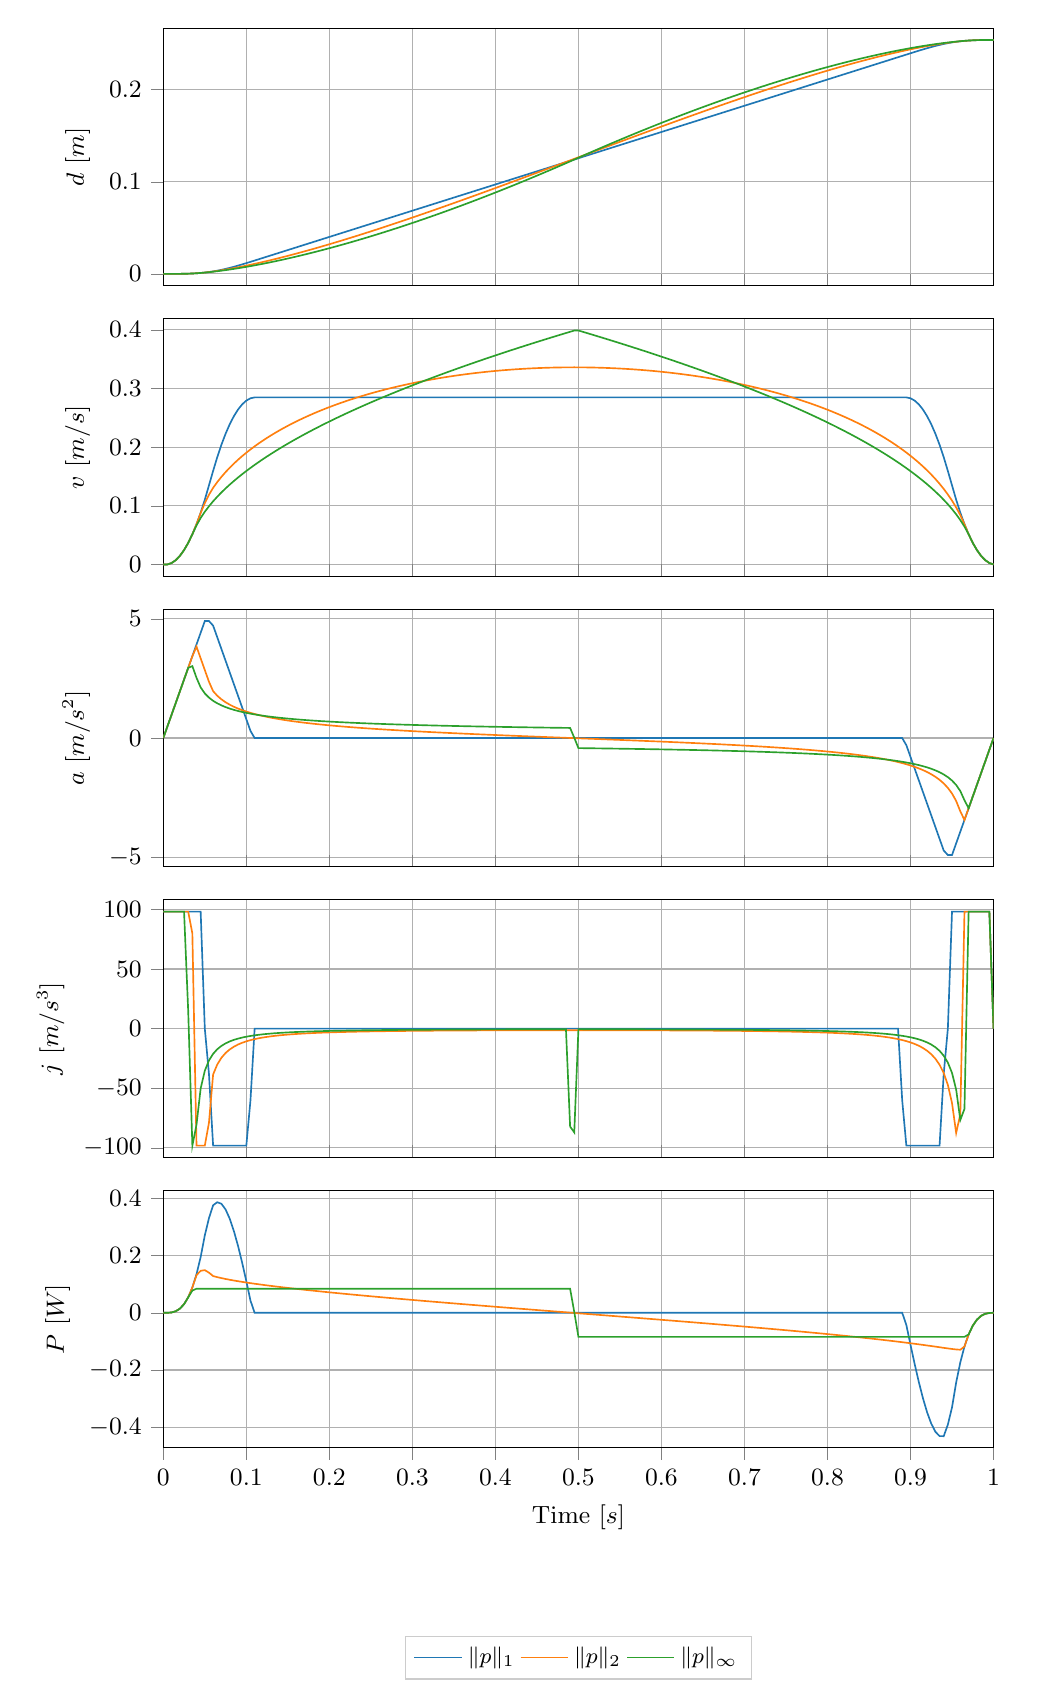
\begin{tikzpicture}

\definecolor{color0}{rgb}{0.12156862745098,0.466666666666667,0.705882352941177}
\definecolor{color1}{rgb}{1,0.498039215686275,0.0549019607843137}
\definecolor{color2}{rgb}{0.172549019607843,0.627450980392157,0.172549019607843}

\begin{groupplot}[group style={group size=1 by 5,vertical sep=12}]
\nextgroupplot[
ytick align=outside,
xticklabels={},
tick pos=left,
x grid style={white!69.01960784313725!black},
xmajorgrids,
xmin=0, xmax=1,
y grid style={white!69.01960784313725!black},
ylabel={$d$ [$m$]},
ymajorgrids,
ymin=-0.0127, ymax=0.2667
%title = \footnotesize{Power}
]
\addplot [semithick, color0]
table [row sep=\\]{%
0	0 \\
0.005	9.25695301174221e-47 \\
0.01	-3.64082910620409e-47 \\
0.015	1.22624999390332e-05 \\
0.02	4.9049999748544e-05 \\
0.025	0.00012262499935038 \\
0.03	0.000245249998653829 \\
0.035	0.000429187497551063 \\
0.04	0.000686699995909681 \\
0.045	0.00103004999355919 \\
0.05	0.0014714999902622 \\
0.055	0.00202331248563346 \\
0.06	0.00269774997870274 \\
0.065	0.0034948124710328 \\
0.07	0.00440975325488723 \\
0.075	0.00543030983112396 \\
0.08	0.00654421970022489 \\
0.085	0.00773922036255711 \\
0.09	0.00900304931844182 \\
0.095	0.0103234440681873 \\
0.1	0.0116881421121146 \\
0.105	0.0130848809505905 \\
0.11	0.0145013980840956 \\
0.115	0.0159254310134818 \\
0.12	0.017349463943552 \\
0.125	0.0187734968742346 \\
0.13	0.0201975298054713 \\
0.135	0.021621562737213 \\
0.14	0.0230455956694177 \\
0.145	0.0244696286020496 \\
0.15	0.0258936615350772 \\
0.155	0.0273176944684731 \\
0.16	0.028741727402213 \\
0.165	0.0301657603362752 \\
0.17	0.0315897932706402 \\
0.175	0.0330138262052907 \\
0.18	0.0344378591402105 \\
0.185	0.0358618920753853 \\
0.19	0.0372859250108018 \\
0.195	0.0387099579464476 \\
0.2	0.0401339908823117 \\
0.205	0.0415580238183834 \\
0.21	0.0429820567546532 \\
0.215	0.0444060896911119 \\
0.22	0.0458301226277512 \\
0.225	0.047254155564563 \\
0.23	0.0486781885015401 \\
0.235	0.0501022214386753 \\
0.24	0.0515262543759621 \\
0.245	0.0529502873133942 \\
0.25	0.0543743202509657 \\
0.255	0.0557983531886709 \\
0.26	0.0572223861265046 \\
0.265	0.0586464190644616 \\
0.27	0.0600704520025371 \\
0.275	0.0614944849407264 \\
0.28	0.0629185178790251 \\
0.285	0.0643425508174289 \\
0.29	0.0657665837559337 \\
0.295	0.0671906166945357 \\
0.3	0.068614649633231 \\
0.305	0.0700386825720159 \\
0.31	0.071462715510887 \\
0.315	0.0728867484498408 \\
0.32	0.0743107813888741 \\
0.325	0.0757348143279836 \\
0.33	0.0771588472671663 \\
0.335	0.0785828802064192 \\
0.34	0.0800069131457394 \\
0.345	0.081430946085124 \\
0.35	0.0828549790245702 \\
0.355	0.0842790119640754 \\
0.36	0.085703044903637 \\
0.365	0.0871270778432524 \\
0.37	0.088551110782919 \\
0.375	0.0899751437226345 \\
0.38	0.0913991766623964 \\
0.385	0.0928232096022024 \\
0.39	0.0942472425420501 \\
0.395	0.0956712754819373 \\
0.4	0.0970953084218617 \\
0.405	0.0985193413618212 \\
0.41	0.0999433743018136 \\
0.415	0.101367407241837 \\
0.42	0.102791440181889 \\
0.425	0.104215473121967 \\
0.43	0.10563950606207 \\
0.435	0.107063539002195 \\
0.44	0.108487571942341 \\
0.445	0.109911604882505 \\
0.45	0.111335637822686 \\
0.455	0.112759670762881 \\
0.46	0.114183703703089 \\
0.465	0.115607736643308 \\
0.47	0.117031769583535 \\
0.475	0.118455802523769 \\
0.48	0.119879835464007 \\
0.485	0.121303868404249 \\
0.49	0.122727901344492 \\
0.495	0.124151934284734 \\
0.5	0.125575967224973 \\
0.505	0.127000000165207 \\
0.51	0.128424033105435 \\
0.515	0.129848066045654 \\
0.52	0.131272098985862 \\
0.525	0.132696131926058 \\
0.53	0.13412016486624 \\
0.535	0.135544197806405 \\
0.54	0.136968230746552 \\
0.545	0.138392263686679 \\
0.55	0.139816296626783 \\
0.555	0.141240329566863 \\
0.56	0.142664362506916 \\
0.565	0.144088395446941 \\
0.57	0.145512428386935 \\
0.575	0.146936461326897 \\
0.58	0.148360494266823 \\
0.585	0.149784527206712 \\
0.59	0.151208560146562 \\
0.595	0.15263259308637 \\
0.6	0.154056626026135 \\
0.605	0.155480658965853 \\
0.61	0.156904691905522 \\
0.615	0.15832872484514 \\
0.62	0.159752757784704 \\
0.625	0.161176790724212 \\
0.63	0.162600823663661 \\
0.635	0.164024856603049 \\
0.64	0.165448889542372 \\
0.645	0.166872922481628 \\
0.65	0.168296955420813 \\
0.655	0.169720988359926 \\
0.66	0.171145021298962 \\
0.665	0.172569054237919 \\
0.67	0.173993087176794 \\
0.675	0.175417120115582 \\
0.68	0.17684115305428 \\
0.685	0.178265185992885 \\
0.69	0.179689218931393 \\
0.695	0.1811132518698 \\
0.7	0.182537284808102 \\
0.705	0.183961317746294 \\
0.71	0.185385350684373 \\
0.715	0.186809383622333 \\
0.72	0.188233416560169 \\
0.725	0.189657449497877 \\
0.73	0.19108148243545 \\
0.735	0.192505515372885 \\
0.74	0.193929548310173 \\
0.745	0.19535358124731 \\
0.75	0.196777614184289 \\
0.755	0.198201647121101 \\
0.76	0.199625680057741 \\
0.765	0.2010497129942 \\
0.77	0.202473745930469 \\
0.775	0.20389777886654 \\
0.78	0.205321811802402 \\
0.785	0.206745844738045 \\
0.79	0.208169877673458 \\
0.795	0.209593910608628 \\
0.8	0.211017943543542 \\
0.805	0.212441976478186 \\
0.81	0.213866009412542 \\
0.815	0.215290042346594 \\
0.82	0.216714075280321 \\
0.825	0.218138108213701 \\
0.83	0.219562141146711 \\
0.835	0.220986174079321 \\
0.84	0.2224102070115 \\
0.845	0.223834239943211 \\
0.85	0.225258272874411 \\
0.855	0.226682305805049 \\
0.86	0.228106338735064 \\
0.865	0.229530371664382 \\
0.87	0.23095440459291 \\
0.875	0.232378437520527 \\
0.88	0.233802470447072 \\
0.885	0.235226503372317 \\
0.89	0.236650536295912 \\
0.895	0.238074569217269 \\
0.9	0.239498602135049 \\
0.905	0.240915119249915 \\
0.91	0.24231185806606 \\
0.915	0.243676556085694 \\
0.92	0.244996950810419 \\
0.925	0.246260779741538 \\
0.93	0.247455780380176 \\
0.935	0.248569690227327 \\
0.94	0.249590246783881 \\
0.945	0.250505187550762 \\
0.95	0.251302250033257 \\
0.955	0.251976687519108 \\
0.96	0.252528500012157 \\
0.965	0.252969950007695 \\
0.97	0.25331330000472 \\
0.975	0.253570812502745 \\
0.98	0.253754750001472 \\
0.985	0.253877375000695 \\
0.99	0.253950950000264 \\
0.995	0.253987737500063 \\
1	0.254 \\
};
\addplot [semithick, color1]
table [row sep=\\]{%
0	0 \\
0.005	-5.55633977183417e-50 \\
0.01	3.72580902032029e-51 \\
0.015	1.22624998764282e-05 \\
0.02	4.90499994794069e-05 \\
0.025	0.000122624998620903 \\
0.03	0.000245249997052825 \\
0.035	0.000429187494420032 \\
0.04	0.000686699990132649 \\
0.045	0.0010300499828061 \\
0.05	0.00146921822598665 \\
0.055	0.00199194222289912 \\
0.06	0.00258595947680784 \\
0.065	0.0032390074950768 \\
0.07	0.00394121879843834 \\
0.075	0.00468778755180045 \\
0.08	0.00547495342989616 \\
0.085	0.00629965947759231 \\
0.09	0.00715935052728483 \\
0.095	0.00805184512284497 \\
0.1	0.00897524946946153 \\
0.105	0.00992789706592706 \\
0.11	0.010908304867537 \\
0.115	0.0119151405416526 \\
0.12	0.0129471974262293 \\
0.125	0.0140033749931337 \\
0.13	0.0150826633425494 \\
0.135	0.0161841307120251 \\
0.14	0.017306913281693 \\
0.145	0.0184502067567998 \\
0.15	0.0196132593457163 \\
0.155	0.0207953658476693 \\
0.16	0.0219958626331133 \\
0.165	0.0232141233495871 \\
0.17	0.0244495552227628 \\
0.175	0.0257015958499914 \\
0.18	0.0269697104045807 \\
0.185	0.0282533891850888 \\
0.19	0.0295521454563683 \\
0.195	0.03086551353884 \\
0.2	0.032193047110178 \\
0.205	0.0335343176897224 \\
0.21	0.0348889132808661 \\
0.215	0.0362564371506503 \\
0.22	0.0376365067290476 \\
0.225	0.0390287526130786 \\
0.23	0.0404328176631017 \\
0.235	0.041848356180436 \\
0.24	0.0432750331569992 \\
0.245	0.0447125235889123 \\
0.25	0.0461605118470958 \\
0.255	0.0476186910987896 \\
0.26	0.0490867627746961 \\
0.265	0.050564436077106 \\
0.27	0.0520514275249267 \\
0.275	0.0535474605320166 \\
0.28	0.0550522650156463 \\
0.285	0.0565655770322672 \\
0.29	0.0580871384380805 \\
0.295	0.0596166965721754 \\
0.3	0.0611540039602374 \\
0.305	0.0626988180370422 \\
0.31	0.0642509008861282 \\
0.315	0.0658100189952058 \\
0.32	0.067375943026 \\
0.325	0.0689484475973512 \\
0.33	0.0705273110805096 \\
0.335	0.0721123154056554 \\
0.34	0.073703245878769 \\
0.345	0.0752998910080489 \\
0.35	0.0769020423391503 \\
0.355	0.0785094942985752 \\
0.36	0.0801220440446041 \\
0.365	0.08173949132521 \\
0.37	0.0833616383424375 \\
0.375	0.0849882896227748 \\
0.38	0.0866192518930808 \\
0.385	0.0882543339616628 \\
0.39	0.0898933466041314 \\
0.395	0.0915361024536849 \\
0.4	0.0931824158955028 \\
0.405	0.0948321029649456 \\
0.41	0.0964849812492839 \\
0.415	0.0981408697926939 \\
0.42	0.0997995890042741 \\
0.425	0.101460960568855 \\
0.43	0.103124807360382 \\
0.435	0.104790953357676 \\
0.44	0.106459223562368 \\
0.445	0.108129443918829 \\
0.45	0.109801441235933 \\
0.455	0.111475043110471 \\
0.46	0.113150077852064 \\
0.465	0.114826374409435 \\
0.47	0.116503762297879 \\
0.475	0.118182071527795 \\
0.48	0.119861132534159 \\
0.485	0.121540776106782 \\
0.49	0.123220833321247 \\
0.495	0.124901135470387 \\
0.5	0.126581513996183 \\
0.505	0.128261800421971 \\
0.51	0.129941826284819 \\
0.515	0.131621423067975 \\
0.52	0.133300422133255 \\
0.525	0.134978654653258 \\
0.53	0.13665595154328 \\
0.535	0.138332143392826 \\
0.54	0.14000706039657 \\
0.545	0.14168053228467 \\
0.55	0.143352388252279 \\
0.555	0.145022456888156 \\
0.56	0.14669056610221 \\
0.565	0.148356543051871 \\
0.57	0.150020214067116 \\
0.575	0.151681404574031 \\
0.58	0.153339939016724 \\
0.585	0.15499564077746 \\
0.59	0.156648332094818 \\
0.595	0.158297833979721 \\
0.6	0.159943966129128 \\
0.605	0.161586546837204 \\
0.61	0.163225392903762 \\
0.615	0.164860319539739 \\
0.62	0.166491140269491 \\
0.625	0.168117666829634 \\
0.63	0.169739709064182 \\
0.635	0.171357074815684 \\
0.64	0.172969569812054 \\
0.645	0.174576997548764 \\
0.65	0.176179159166046 \\
0.655	0.177775853320717 \\
0.66	0.179366876052215 \\
0.665	0.180952020642402 \\
0.67	0.182531077468638 \\
0.675	0.184103833849615 \\
0.68	0.185670073883368 \\
0.685	0.187229578276849 \\
0.69	0.188782124166371 \\
0.695	0.190327484928201 \\
0.7	0.191865429978474 \\
0.705	0.193395724561542 \\
0.71	0.19491812952578 \\
0.715	0.196432401085782 \\
0.72	0.197938290569742 \\
0.725	0.19943554415073 \\
0.73	0.200923902560397 \\
0.735	0.202403100783516 \\
0.74	0.203872867731559 \\
0.745	0.205332925893319 \\
0.75	0.206782990960373 \\
0.755	0.208222771424879 \\
0.76	0.209651968146931 \\
0.765	0.211070273888333 \\
0.77	0.212477372809271 \\
0.775	0.213872939923867 \\
0.78	0.215256640510116 \\
0.785	0.21662812946904 \\
0.79	0.217987050627215 \\
0.795	0.219333035975936 \\
0.8	0.220665704839342 \\
0.805	0.221984662962621 \\
0.81	0.223289501510037 \\
0.815	0.224579795960891 \\
0.82	0.225855104889534 \\
0.825	0.227114968613197 \\
0.83	0.22835890768857 \\
0.835	0.229586421234542 \\
0.84	0.230796985054342 \\
0.845	0.231990049525067 \\
0.85	0.233165037216176 \\
0.855	0.234321340190474 \\
0.86	0.235458316931072 \\
0.865	0.236575288825004 \\
0.87	0.237671536117921 \\
0.875	0.238746293233267 \\
0.88	0.239798743321964 \\
0.885	0.240828011872618 \\
0.89	0.241833159164217 \\
0.895	0.242813171278452 \\
0.9	0.243766949299942 \\
0.905	0.244693296209028 \\
0.91	0.245590900796763 \\
0.915	0.246458317679002 \\
0.92	0.247293942113734 \\
0.925	0.248095977762375 \\
0.93	0.248862394660362 \\
0.935	0.249590873258921 \\
0.94	0.250278728066236 \\
0.945	0.250922800367833 \\
0.95	0.251519302119785 \\
0.955	0.252063578789677 \\
0.96	0.252549729005873 \\
0.965	0.252969950023096 \\
0.97	0.253313300010803 \\
0.975	0.253570812505784 \\
0.98	0.253754750002971 \\
0.985	0.253877375001366 \\
0.99	0.25395095000051 \\
0.995	0.25398773750012 \\
1	0.254 \\
};
\addplot [semithick, color2]
table [row sep=\\]{%
0	0 \\
0.005	5.45021791331394e-42 \\
0.01	-2.40380353859081e-30 \\
0.015	1.22624954347334e-05 \\
0.02	4.90499807082241e-05 \\
0.025	0.000122624948671972 \\
0.03	0.000245249889580744 \\
0.035	0.000429187288481109 \\
0.04	0.000686699614763461 \\
0.045	0.00101962428676764 \\
0.05	0.00141569883661211 \\
0.055	0.00186485466884201 \\
0.06	0.00236081863029006 \\
0.065	0.00289917305795396 \\
0.07	0.00347658009083621 \\
0.075	0.00409039842657789 \\
0.08	0.00473846816955753 \\
0.085	0.00541897908336943 \\
0.09	0.00613038463866607 \\
0.095	0.00687134315432883 \\
0.1	0.00764067591660535 \\
0.105	0.00843733643633536 \\
0.11	0.00926038729182438 \\
0.115	0.0101089823016406 \\
0.12	0.0109823525426262 \\
0.125	0.0118797952056053 \\
0.13	0.0128006645868787 \\
0.135	0.0137443647151878 \\
0.14	0.0147103432502735 \\
0.145	0.0156980863836372 \\
0.15	0.0167071145388531 \\
0.155	0.0177369787168054 \\
0.16	0.0187872573663231 \\
0.165	0.0198575536867389 \\
0.17	0.02094749328848 \\
0.175	0.0220567221527096 \\
0.18	0.0231849048425093 \\
0.185	0.0243317229270179 \\
0.19	0.0254968735869478 \\
0.195	0.0266800683754468 \\
0.2	0.027881032112707 \\
0.205	0.0290995018962858 \\
0.21	0.0303352262119936 \\
0.215	0.0315879641325607 \\
0.22	0.0328574845932311 \\
0.225	0.0341435657350277 \\
0.23	0.0354459943077619 \\
0.235	0.0367645651259665 \\
0.24	0.0380990805718618 \\
0.245	0.0394493501402457 \\
0.25	0.0408151900208631 \\
0.255	0.0421964227143725 \\
0.26	0.0435928766785078 \\
0.265	0.0450043860014485 \\
0.27	0.0464307900997597 \\
0.275	0.0478719334385765 \\
0.28	0.0493276652719646 \\
0.285	0.050797839401625 \\
0.29	0.0522823139523049 \\
0.295	0.0537809511624575 \\
0.3	0.0552936171888417 \\
0.305	0.0568201819238893 \\
0.31	0.0583605188247874 \\
0.315	0.0599145047533236 \\
0.32	0.0614820198256391 \\
0.325	0.0630629472711135 \\
0.33	0.0646571732996796 \\
0.335	0.0662645869769302 \\
0.34	0.0678850801064385 \\
0.345	0.0695185471187634 \\
0.35	0.0711648849666598 \\
0.355	0.0728239930260534 \\
0.36	0.0744957730023776 \\
0.365	0.0761801288419059 \\
0.37	0.0778769666477399 \\
0.375	0.0795861946001432 \\
0.38	0.0813077228809357 \\
0.385	0.0830414636016847 \\
0.39	0.0847873307354504 \\
0.395	0.0865452400518608 \\
0.4	0.0883151090553093 \\
0.405	0.0900968569260815 \\
0.41	0.0918904044642335 \\
0.415	0.0936956740360552 \\
0.42	0.0955125895229622 \\
0.425	0.0973410762726727 \\
0.43	0.0991810610525302 \\
0.435	0.101032472004844 \\
0.44	0.102895238604117 \\
0.445	0.104769291616045 \\
0.45	0.106654563058154 \\
0.455	0.108550986161939 \\
0.46	0.110458495336356 \\
0.465	0.11237702613245 \\
0.47	0.114306515208813 \\
0.475	0.11624690029734 \\
0.48	0.11819812016818 \\
0.485	0.120160114591255 \\
0.49	0.122132824286573 \\
0.495	0.124116190832349 \\
0.5	0.12611015631484 \\
0.505	0.128104458941858 \\
0.51	0.130088220765054 \\
0.515	0.13206138511681 \\
0.52	0.134023894859175 \\
0.525	0.135975692036344 \\
0.53	0.137916717784641 \\
0.535	0.139846912284686 \\
0.54	0.141766214724841 \\
0.545	0.143674563268192 \\
0.55	0.145571895020445 \\
0.555	0.147458145997642 \\
0.56	0.149333251093178 \\
0.565	0.151197144043815 \\
0.57	0.153049757394503 \\
0.575	0.154891022461842 \\
0.58	0.156720869296087 \\
0.585	0.15853922664156 \\
0.59	0.16034602189537 \\
0.595	0.162141181064329 \\
0.6	0.163924628719946 \\
0.605	0.165696287951382 \\
0.61	0.167456080316236 \\
0.615	0.169203925789039 \\
0.62	0.170939742707294 \\
0.625	0.172663447714921 \\
0.63	0.174374955702948 \\
0.635	0.176074179747245 \\
0.64	0.177761031043146 \\
0.645	0.179435418836716 \\
0.65	0.181097250352472 \\
0.655	0.18274643071729 \\
0.66	0.184382862880256 \\
0.665	0.186006447528172 \\
0.67	0.187617082996396 \\
0.675	0.189214665174709 \\
0.68	0.190799087407811 \\
0.685	0.192370240390079 \\
0.69	0.193928012054124 \\
0.695	0.195472287452697 \\
0.7	0.197002948633408 \\
0.705	0.198519874505685 \\
0.71	0.200022940699364 \\
0.715	0.20151201941419 \\
0.72	0.202986979259498 \\
0.725	0.204447685083208 \\
0.73	0.205893997789219 \\
0.735	0.207325774142163 \\
0.74	0.208742866558373 \\
0.745	0.210145122881796 \\
0.75	0.211532386143415 \\
0.755	0.212904494302607 \\
0.76	0.214261279968639 \\
0.765	0.215602570100312 \\
0.77	0.216928185681494 \\
0.775	0.218237941370003 \\
0.78	0.21953164511696 \\
0.785	0.220809097753339 \\
0.79	0.222070092540003 \\
0.795	0.223314414676979 \\
0.8	0.22454184076709 \\
0.805	0.225752138228364 \\
0.81	0.226945064648756 \\
0.815	0.228120367075703 \\
0.82	0.229277781231814 \\
0.825	0.23041703064654 \\
0.83	0.231537825691903 \\
0.835	0.232639862508239 \\
0.84	0.233722821803315 \\
0.845	0.234786367504998 \\
0.85	0.235830145243732 \\
0.855	0.236853780636219 \\
0.86	0.237856877335582 \\
0.865	0.238839014805611 \\
0.87	0.239799745766918 \\
0.875	0.240738593250218 \\
0.88	0.241655047175708 \\
0.885	0.242548560356084 \\
0.89	0.243418543792427 \\
0.895	0.244264361094052 \\
0.9	0.245085321801497 \\
0.905	0.245880673319963 \\
0.91	0.246649591069348 \\
0.915	0.247391166311863 \\
0.92	0.248104390905512 \\
0.925	0.24878813791251 \\
0.93	0.249441136499412 \\
0.935	0.250061938782871 \\
0.94	0.250648874984248 \\
0.945	0.251199991037768 \\
0.95	0.251712958788762 \\
0.955	0.252184941229656 \\
0.96	0.252612379338142 \\
0.965	0.252990631043532 \\
0.97	0.253313300333528 \\
0.975	0.253570812683426 \\
0.98	0.253754750095869 \\
0.985	0.25387737504461 \\
0.99	0.253950950016782 \\
0.995	0.253987737503974 \\
1	0.254 \\
};
\nextgroupplot[
ytick align=outside,
xticklabels={},
tick pos=left,
x grid style={white!69.01960784313725!black},
xmajorgrids,
xmin=0, xmax=1,
y grid style={white!69.01960784313725!black},
ylabel={$v$ [$m/s$]},
ymajorgrids,
ymin=-0.0199430262701768, ymax=0.418803551673712
]
\addplot [semithick, color0, forget plot]
table [row sep=\\]{%
0	1.93501887858559e-44 \\
0.005	0 \\
0.01	0.00245249998780663 \\
0.015	0.00735749996190217 \\
0.02	0.0147149999203671 \\
0.025	0.0245249998606899 \\
0.03	0.0367874997794469 \\
0.035	0.0515024996717235 \\
0.04	0.068669999529902 \\
0.045	0.0882899993406014 \\
0.05	0.110362499074252 \\
0.055	0.134887498613855 \\
0.06	0.159412498466013 \\
0.065	0.182988156770885 \\
0.07	0.204111315247347 \\
0.075	0.222781973820185 \\
0.08	0.239000132466444 \\
0.085	0.252765791176941 \\
0.09	0.264078949949097 \\
0.095	0.272939608785463 \\
0.1	0.279347767695171 \\
0.105	0.283303426701025 \\
0.11	0.28480658587724 \\
0.115	0.284806586014034 \\
0.12	0.284806586136526 \\
0.125	0.284806586247343 \\
0.13	0.284806586348329 \\
0.135	0.284806586440951 \\
0.14	0.28480658652637 \\
0.145	0.284806586605524 \\
0.15	0.284806586679181 \\
0.155	0.284806586747977 \\
0.16	0.28480658681244 \\
0.165	0.284806586873016 \\
0.17	0.284806586930085 \\
0.175	0.284806586983972 \\
0.18	0.284806587034958 \\
0.185	0.284806587083287 \\
0.19	0.284806587129174 \\
0.195	0.284806587172805 \\
0.2	0.284806587214349 \\
0.205	0.284806587253953 \\
0.21	0.284806587291748 \\
0.215	0.284806587327853 \\
0.22	0.284806587362375 \\
0.225	0.28480658739541 \\
0.23	0.284806587427044 \\
0.235	0.284806587457356 \\
0.24	0.284806587486418 \\
0.245	0.284806587514296 \\
0.25	0.28480658754105 \\
0.255	0.284806587566735 \\
0.26	0.284806587591402 \\
0.265	0.284806587615096 \\
0.27	0.284806587637862 \\
0.275	0.284806587659739 \\
0.28	0.284806587680764 \\
0.285	0.28480658770097 \\
0.29	0.28480658772039 \\
0.295	0.284806587739053 \\
0.3	0.284806587756986 \\
0.305	0.284806587774215 \\
0.31	0.284806587790764 \\
0.315	0.284806587806655 \\
0.32	0.284806587821908 \\
0.325	0.284806587836543 \\
0.33	0.284806587850579 \\
0.335	0.284806587864031 \\
0.34	0.284806587876917 \\
0.345	0.28480658788925 \\
0.35	0.284806587901046 \\
0.355	0.284806587912316 \\
0.36	0.284806587923073 \\
0.365	0.284806587933329 \\
0.37	0.284806587943095 \\
0.375	0.284806587952379 \\
0.38	0.284806587961193 \\
0.385	0.284806587969544 \\
0.39	0.28480658797744 \\
0.395	0.28480658798489 \\
0.4	0.284806587991901 \\
0.405	0.284806587998478 \\
0.41	0.284806588004629 \\
0.415	0.284806588010358 \\
0.42	0.284806588015672 \\
0.425	0.284806588020574 \\
0.43	0.284806588025069 \\
0.435	0.284806588029162 \\
0.44	0.284806588032855 \\
0.445	0.284806588036152 \\
0.45	0.284806588039057 \\
0.455	0.28480658804157 \\
0.46	0.284806588043695 \\
0.465	0.284806588045433 \\
0.47	0.284806588046786 \\
0.475	0.284806588047755 \\
0.48	0.284806588048341 \\
0.485	0.284806588048544 \\
0.49	0.284806588048364 \\
0.495	0.284806588047801 \\
0.5	0.284806588046855 \\
0.505	0.284806588045525 \\
0.51	0.28480658804381 \\
0.515	0.284806588041707 \\
0.52	0.284806588039217 \\
0.525	0.284806588036335 \\
0.53	0.28480658803306 \\
0.535	0.284806588029389 \\
0.54	0.284806588025318 \\
0.545	0.284806588020845 \\
0.55	0.284806588015964 \\
0.555	0.284806588010672 \\
0.56	0.284806588004964 \\
0.565	0.284806587998834 \\
0.57	0.284806587992277 \\
0.575	0.284806587985286 \\
0.58	0.284806587977856 \\
0.585	0.284806587969979 \\
0.59	0.284806587961646 \\
0.595	0.284806587952851 \\
0.6	0.284806587943584 \\
0.605	0.284806587933835 \\
0.61	0.284806587923596 \\
0.615	0.284806587912854 \\
0.62	0.284806587901598 \\
0.625	0.284806587889817 \\
0.63	0.284806587877496 \\
0.635	0.284806587864622 \\
0.64	0.284806587851181 \\
0.645	0.284806587837155 \\
0.65	0.284806587822528 \\
0.655	0.284806587807282 \\
0.66	0.284806587791396 \\
0.665	0.284806587774851 \\
0.67	0.284806587757624 \\
0.675	0.28480658773969 \\
0.68	0.284806587721025 \\
0.685	0.2848065877016 \\
0.69	0.284806587681386 \\
0.695	0.284806587660351 \\
0.7	0.284806587638461 \\
0.705	0.284806587615678 \\
0.71	0.284806587591962 \\
0.715	0.28480658756727 \\
0.72	0.284806587541555 \\
0.725	0.284806587514766 \\
0.73	0.284806587486846 \\
0.735	0.284806587457736 \\
0.74	0.284806587427368 \\
0.745	0.284806587395671 \\
0.75	0.284806587362563 \\
0.755	0.284806587327958 \\
0.76	0.284806587291758 \\
0.765	0.284806587253854 \\
0.77	0.284806587214126 \\
0.775	0.284806587172441 \\
0.78	0.284806587128648 \\
0.785	0.284806587082577 \\
0.79	0.284806587034037 \\
0.795	0.28480658698281 \\
0.8	0.284806586928645 \\
0.805	0.284806586871256 \\
0.81	0.28480658681031 \\
0.815	0.284806586745418 \\
0.82	0.284806586676122 \\
0.825	0.284806586601879 \\
0.83	0.284806586522035 \\
0.835	0.284806586435796 \\
0.84	0.284806586342185 \\
0.845	0.284806586239976 \\
0.85	0.284806586127612 \\
0.855	0.284806586003062 \\
0.86	0.284806585863613 \\
0.865	0.284806585705521 \\
0.87	0.284806585523396 \\
0.875	0.284806585309031 \\
0.88	0.284806585048956 \\
0.885	0.284806584719061 \\
0.89	0.284806584271436 \\
0.895	0.284806583556055 \\
0.9	0.283303422973131 \\
0.905	0.27934776322908 \\
0.91	0.272939603926665 \\
0.915	0.264078944944966 \\
0.92	0.252765786223985 \\
0.925	0.239000127727573 \\
0.93	0.222781969430172 \\
0.935	0.20411131131084 \\
0.94	0.182988153376127 \\
0.945	0.159412496499095 \\
0.95	0.134887497170097 \\
0.955	0.110362498609733 \\
0.96	0.0882899991076826 \\
0.965	0.068669999405065 \\
0.97	0.051502499605017 \\
0.975	0.0367874997452947 \\
0.98	0.0245249998445884 \\
0.985	0.0147149999137768 \\
0.99	0.00735749995981772 \\
0.995	0.00245249998743795 \\
1	0 \\
};
\addplot [semithick, color1, forget plot]
table [row sep=\\]{%
0	0 \\
0.005	0 \\
0.01	0.00245249997528564 \\
0.015	0.00735749992059574 \\
0.02	0.0147149998282992 \\
0.025	0.0245249996863844 \\
0.03	0.0367874994734413 \\
0.035	0.0515024991425235 \\
0.04	0.0686699985346907 \\
0.045	0.0878336486361088 \\
0.05	0.104544799382495 \\
0.055	0.118803450781744 \\
0.06	0.130609603653792 \\
0.065	0.140442260672308 \\
0.07	0.149313750672421 \\
0.075	0.157433175619143 \\
0.08	0.16494120953923 \\
0.085	0.171938209938502 \\
0.09	0.178498919112028 \\
0.095	0.184680869323313 \\
0.1	0.190529519293105 \\
0.105	0.196081560321998 \\
0.11	0.201367134823114 \\
0.115	0.206411376915327 \\
0.12	0.211235513380896 \\
0.125	0.215857669883125 \\
0.13	0.220293473895152 \\
0.135	0.224556513933583 \\
0.14	0.22865869502136 \\
0.145	0.232610517783298 \\
0.15	0.236421300390591 \\
0.155	0.240099357088795 \\
0.16	0.243652143294777 \\
0.165	0.247086374635125 \\
0.17	0.250408125445723 \\
0.175	0.253622910917866 \\
0.18	0.256735756101624 \\
0.185	0.259751254255889 \\
0.19	0.262673616494343 \\
0.195	0.265506714267605 \\
0.2	0.268254115908868 \\
0.205	0.270919118228753 \\
0.21	0.27350477395684 \\
0.215	0.27601391567945 \\
0.22	0.278449176806211 \\
0.225	0.280813010004621 \\
0.23	0.28310770346686 \\
0.235	0.285335395312638 \\
0.24	0.287498086382607 \\
0.245	0.28959765163671 \\
0.25	0.291635850338766 \\
0.255	0.293614335181298 \\
0.26	0.295534660481977 \\
0.265	0.297398289564129 \\
0.27	0.29920660141798 \\
0.275	0.300960896725954 \\
0.28	0.302662403324166 \\
0.285	0.304312281162667 \\
0.29	0.305911626818971 \\
0.295	0.307461477612403 \\
0.3	0.308962815360955 \\
0.305	0.310416569817213 \\
0.31	0.311823621815523 \\
0.315	0.313184806158828 \\
0.32	0.314500914270245 \\
0.325	0.315772696631673 \\
0.33	0.317000865029171 \\
0.335	0.318186094622712 \\
0.34	0.319329025855988 \\
0.345	0.320430266220285 \\
0.35	0.321490391884965 \\
0.355	0.32250994920579 \\
0.36	0.323489456121179 \\
0.365	0.32442940344549 \\
0.37	0.325330256067458 \\
0.375	0.326192454061203 \\
0.38	0.327016413716408 \\
0.385	0.327802528493708 \\
0.39	0.328551169910713 \\
0.395	0.329262688363572 \\
0.4	0.329937413888555 \\
0.405	0.330575656867672 \\
0.41	0.331177708682 \\
0.415	0.331743842316037 \\
0.42	0.332274312916099 \\
0.425	0.332769358305483 \\
0.43	0.333229199458872 \\
0.435	0.333654040938232 \\
0.44	0.334044071292213 \\
0.445	0.334399463420894 \\
0.45	0.334720374907513 \\
0.455	0.335006948318669 \\
0.46	0.335259311474304 \\
0.465	0.335477577688665 \\
0.47	0.335661845983264 \\
0.475	0.335812201272773 \\
0.48	0.335928714524625 \\
0.485	0.33601144289302 \\
0.49	0.336060429827887 \\
0.495	0.336075705159276 \\
0.5	0.336057285157541 \\
0.505	0.336005172569569 \\
0.51	0.335919356631229 \\
0.515	0.335799813056102 \\
0.52	0.335646504000476 \\
0.525	0.335459378004475 \\
0.53	0.335238369909111 \\
0.535	0.334983400748942 \\
0.54	0.33469437761992 \\
0.545	0.334371193521922 \\
0.55	0.334013727175317 \\
0.555	0.333621842810868 \\
0.56	0.333195389932089 \\
0.565	0.3327342030491 \\
0.57	0.332238101382879 \\
0.575	0.331706888538662 \\
0.58	0.331140352147111 \\
0.585	0.330538263471702 \\
0.59	0.329900376980621 \\
0.595	0.329226429881263 \\
0.6	0.328516141615239 \\
0.605	0.327769213311577 \\
0.61	0.326985327195557 \\
0.615	0.326164145950375 \\
0.62	0.325305312028544 \\
0.625	0.324408446909608 \\
0.63	0.323473150300449 \\
0.635	0.322498999274024 \\
0.64	0.321485547342015 \\
0.645	0.320432323456352 \\
0.65	0.319338830934113 \\
0.655	0.318204546299667 \\
0.66	0.317028918037343 \\
0.665	0.315811365247167 \\
0.67	0.314551276195403 \\
0.675	0.313248006750757 \\
0.68	0.311900878696086 \\
0.685	0.310509177904323 \\
0.69	0.309072152366039 \\
0.695	0.307589010054639 \\
0.7	0.306058916613531 \\
0.705	0.304480992847754 \\
0.71	0.30285431200043 \\
0.715	0.301177896792001 \\
0.72	0.299450716197431 \\
0.725	0.297671681933411 \\
0.73	0.295839644623937 \\
0.735	0.293953389608468 \\
0.74	0.292011632352011 \\
0.745	0.29001301341086 \\
0.75	0.287956092901217 \\
0.755	0.285839344410286 \\
0.76	0.283661148280561 \\
0.765	0.281419784187594 \\
0.77	0.27911342291921 \\
0.775	0.276740117249656 \\
0.78	0.274297791784932 \\
0.785	0.27178423163501 \\
0.79	0.269197069744176 \\
0.795	0.266533772681219 \\
0.8	0.26379162465567 \\
0.805	0.260967709483219 \\
0.81	0.25805889017091 \\
0.815	0.255061785728441 \\
0.82	0.251972744732703 \\
0.825	0.248787815074537 \\
0.83	0.245502709194384 \\
0.835	0.242112763959971 \\
0.84	0.238612894145116 \\
0.845	0.234997538221693 \\
0.85	0.231260594859671 \\
0.855	0.227395348119671 \\
0.86	0.223394378786318 \\
0.865	0.219249458583411 \\
0.87	0.214951423069233 \\
0.875	0.210490017739455 \\
0.88	0.205853710130757 \\
0.885	0.201029458319804 \\
0.89	0.196002422847027 \\
0.895	0.190755604297881 \\
0.9	0.185269381817188 \\
0.905	0.179520917547067 \\
0.91	0.173483376447793 \\
0.915	0.167124886946432 \\
0.92	0.160407129728075 \\
0.925	0.1532833795975 \\
0.93	0.145695719711703 \\
0.935	0.137570961463109 \\
0.94	0.128814460319352 \\
0.945	0.119300350390417 \\
0.95	0.108855333978357 \\
0.955	0.0972300432392828 \\
0.96	0.0840442034445907 \\
0.965	0.0686699975413425 \\
0.97	0.0515024989963208 \\
0.975	0.036787499437366 \\
0.98	0.0245249996790202 \\
0.985	0.0147149998286512 \\
0.99	0.00735749992206043 \\
0.995	0.00245249997602257 \\
1	0 \\
};
\addplot [semithick, color2, forget plot]
table [row sep=\\]{%
0	1.09004358266264e-39 \\
0.005	0 \\
0.01	0.00245249908694667 \\
0.015	0.00735749705469815 \\
0.02	0.0147149935927495 \\
0.025	0.0245249881817544 \\
0.03	0.0367874797800731 \\
0.035	0.0515024652564704 \\
0.04	0.066584934400836 \\
0.045	0.0792149099688938 \\
0.05	0.0898311664459793 \\
0.055	0.0991927922896105 \\
0.06	0.107670885532781 \\
0.065	0.115481406576449 \\
0.07	0.122763667148337 \\
0.075	0.129613948595927 \\
0.08	0.136102182762381 \\
0.085	0.142281111059328 \\
0.09	0.148191703132551 \\
0.095	0.153866552455304 \\
0.1	0.159332103946002 \\
0.105	0.164610171097805 \\
0.11	0.169719001963238 \\
0.115	0.174674048197125 \\
0.12	0.179488532595818 \\
0.125	0.184173876254692 \\
0.13	0.188740025661808 \\
0.135	0.193195707017152 \\
0.14	0.197548626672721 \\
0.145	0.201805631043186 \\
0.15	0.205972835590461 \\
0.155	0.210055729903547 \\
0.16	0.214059264083151 \\
0.165	0.217987920348222 \\
0.17	0.221845772845925 \\
0.175	0.225636537959936 \\
0.18	0.22936361690173 \\
0.185	0.233030131985975 \\
0.19	0.23663895769979 \\
0.195	0.240192747452044 \\
0.2	0.243693956715766 \\
0.205	0.247144863141556 \\
0.21	0.25054758411342 \\
0.215	0.253904092134078 \\
0.22	0.257216228359325 \\
0.225	0.260485714546835 \\
0.23	0.263714163640921 \\
0.235	0.266903089179059 \\
0.24	0.270053913676782 \\
0.245	0.273167976123489 \\
0.25	0.276246538701866 \\
0.255	0.279290792827077 \\
0.26	0.282301864588131 \\
0.265	0.285280819662243 \\
0.27	0.288228667763347 \\
0.275	0.29114636667763 \\
0.28	0.294034825932071 \\
0.285	0.296894910135985 \\
0.29	0.299727442030531 \\
0.295	0.302533205276825 \\
0.3	0.305312947009529 \\
0.305	0.308067380179621 \\
0.31	0.310797185707239 \\
0.315	0.313503014463097 \\
0.32	0.316185489094886 \\
0.325	0.318845205713218 \\
0.33	0.321482735450121 \\
0.335	0.324098625901648 \\
0.34	0.326693402464982 \\
0.345	0.329267569579295 \\
0.35	0.331821611878708 \\
0.355	0.334355995264839 \\
0.36	0.336871167905666 \\
0.365	0.339367561166799 \\
0.37	0.341845590480656 \\
0.375	0.344305656158494 \\
0.38	0.346748144149803 \\
0.385	0.349173426753141 \\
0.39	0.351581863282089 \\
0.395	0.353973800689697 \\
0.4	0.356349574154434 \\
0.405	0.358709507630412 \\
0.41	0.361053914364334 \\
0.415	0.3633830973814 \\
0.42	0.365697349942089 \\
0.425	0.367996955971518 \\
0.43	0.370282190462697 \\
0.435	0.37255331985464 \\
0.44	0.374810602385711 \\
0.445	0.377054288421739 \\
0.45	0.379284620756981 \\
0.455	0.381501834883421 \\
0.46	0.383706159218769 \\
0.465	0.385897815272666 \\
0.47	0.388077017705395 \\
0.475	0.390243974167855 \\
0.48	0.392398884615004 \\
0.485	0.394541939063663 \\
0.49	0.396673309155184 \\
0.495	0.398793096498303 \\
0.5	0.398860525403535 \\
0.505	0.396752364639186 \\
0.51	0.394632870351177 \\
0.515	0.392501948473061 \\
0.52	0.390359435433713 \\
0.525	0.388205149659458 \\
0.53	0.386038900008983 \\
0.535	0.383860488030923 \\
0.54	0.38166970867029 \\
0.545	0.379466350450644 \\
0.55	0.377250195439348 \\
0.555	0.375021019107109 \\
0.56	0.372778590127566 \\
0.565	0.370522670137557 \\
0.57	0.368253013467847 \\
0.575	0.365969366849005 \\
0.58	0.363671469094545 \\
0.585	0.361359050762004 \\
0.59	0.359031833791837 \\
0.595	0.356689531123409 \\
0.6	0.354331846287063 \\
0.605	0.351958472970893 \\
0.61	0.349569094560639 \\
0.615	0.347163383650886 \\
0.62	0.34474100152553 \\
0.625	0.342301597605246 \\
0.63	0.339844808859467 \\
0.635	0.337370259180123 \\
0.64	0.33487755871411 \\
0.645	0.332366303151175 \\
0.65	0.32983607296355 \\
0.655	0.327286432593311 \\
0.66	0.324716929583036 \\
0.665	0.322127093644862 \\
0.67	0.319516435662544 \\
0.675	0.316884446620542 \\
0.68	0.31423059645353 \\
0.685	0.311554332808979 \\
0.69	0.308855079714675 \\
0.695	0.306132236142096 \\
0.7	0.303385174455544 \\
0.705	0.300613238735742 \\
0.71	0.297815742965253 \\
0.715	0.294991969061571 \\
0.72	0.292141164741969 \\
0.725	0.289262541202184 \\
0.73	0.286355270588748 \\
0.735	0.283418483242097 \\
0.74	0.28045126468457 \\
0.745	0.277452652323858 \\
0.75	0.27442163183839 \\
0.755	0.271357133206352 \\
0.76	0.268258026334505 \\
0.765	0.265123116236395 \\
0.77	0.261951137701957 \\
0.775	0.25874074939141 \\
0.78	0.255490527275687 \\
0.785	0.252198957332907 \\
0.79	0.248864427395216 \\
0.795	0.245485218022155 \\
0.8	0.242059492254797 \\
0.805	0.238585284078432 \\
0.81	0.235060485389379 \\
0.815	0.231482831222187 \\
0.82	0.227849882945174 \\
0.825	0.224159009072557 \\
0.83	0.220407363267211 \\
0.835	0.216591859015241 \\
0.84	0.212709140336517 \\
0.845	0.208755547746848 \\
0.85	0.204727078497462 \\
0.855	0.20061933987245 \\
0.86	0.196427494005886 \\
0.865	0.192146192261333 \\
0.87	0.187769496660112 \\
0.875	0.183290785097967 \\
0.88	0.178702636075174 \\
0.885	0.173996687268662 \\
0.89	0.169163460325058 \\
0.895	0.164192141488954 \\
0.9	0.159070303693173 \\
0.905	0.153783549877025 \\
0.91	0.148315048502869 \\
0.915	0.142644918729983 \\
0.92	0.136749401399531 \\
0.925	0.13059971738044 \\
0.93	0.124160456691706 \\
0.935	0.117387240275482 \\
0.94	0.110223210703969 \\
0.945	0.102593550198805 \\
0.95	0.0943964881788538 \\
0.955	0.0854876216971342 \\
0.96	0.0756503410779507 \\
0.965	0.0645338579992773 \\
0.97	0.0515024699795693 \\
0.975	0.0367874824886742 \\
0.98	0.0245249897480518 \\
0.985	0.0147149944343828 \\
0.99	0.00735749743856703 \\
0.995	0.00245249920510985 \\
1	0 \\
};
\nextgroupplot[
ytick align=outside,
xticklabels={},
tick pos=left,
x grid style={white!69.01960784313725!black},
xmajorgrids,
xmin=0, xmax=1,
y grid style={white!69.01960784313725!black},
ylabel={$a$ [$m/s^2$]},
ymajorgrids,
ymin=-5.3954998576111, ymax=5.39549996224311
]
\addplot [semithick, color0, forget plot]
table [row sep=\\]{%
0	0 \\
0.005	0.490499997561326 \\
0.01	0.980999994819107 \\
0.015	1.47149999169299 \\
0.02	1.96199998806456 \\
0.025	2.45249998375139 \\
0.03	2.94299997845532 \\
0.035	3.4334999716357 \\
0.04	3.92399996213988 \\
0.045	4.4144999467302 \\
0.05	4.90499990792058 \\
0.055	4.90499997043155 \\
0.06	4.71513166097447 \\
0.065	4.22463169529226 \\
0.07	3.73413171456776 \\
0.075	3.24363172925178 \\
0.08	2.75313174209937 \\
0.085	2.2626317544312 \\
0.09	1.77213176727313 \\
0.095	1.28163178194157 \\
0.1	0.791131801170949 \\
0.105	0.300631835242886 \\
0.11	2.73588391525873e-08 \\
0.115	2.44983597633741e-08 \\
0.12	2.21634052543417e-08 \\
0.125	2.01971265256757e-08 \\
0.13	1.85244759380757e-08 \\
0.135	1.70837629147087e-08 \\
0.14	1.58308114406532e-08 \\
0.145	1.47315337611539e-08 \\
0.15	1.37591345125667e-08 \\
0.155	1.28925887621273e-08 \\
0.16	1.21152503636926e-08 \\
0.165	1.14137815185861e-08 \\
0.17	1.07773713210053e-08 \\
0.175	1.01971646812819e-08 \\
0.18	9.66583921400324e-09 \\
0.185	9.17728726386785e-09 \\
0.19	8.72637385422624e-09 \\
0.195	8.3087502615343e-09 \\
0.2	7.92070887442145e-09 \\
0.205	7.55906905940687e-09 \\
0.21	7.22108657333389e-09 \\
0.215	6.90438104296786e-09 \\
0.22	6.60687744195334e-09 \\
0.225	6.32675850993683e-09 \\
0.23	6.06242579800181e-09 \\
0.235	5.81246756827909e-09 \\
0.24	5.57563218009711e-09 \\
0.245	5.35080589821252e-09 \\
0.25	5.13699428846714e-09 \\
0.255	4.93330654158911e-09 \\
0.26	4.73894220081516e-09 \\
0.265	4.55317987354044e-09 \\
0.27	4.37536758909534e-09 \\
0.275	4.20491452883966e-09 \\
0.28	4.04128390568979e-09 \\
0.285	3.88398681052182e-09 \\
0.29	3.73257687541244e-09 \\
0.295	3.58664562956529e-09 \\
0.3	3.44581844495934e-09 \\
0.305	3.30975098585237e-09 \\
0.31	3.17812609019999e-09 \\
0.315	3.05065102260122e-09 \\
0.32	2.92705504778917e-09 \\
0.325	2.80708728151455e-09 \\
0.33	2.69051478212703e-09 \\
0.335	2.57712085166304e-09 \\
0.34	2.4667035196454e-09 \\
0.345	2.35907418672985e-09 \\
0.35	2.25405640842463e-09 \\
0.355	2.15148480189153e-09 \\
0.36	2.05120406110831e-09 \\
0.365	1.95306806756649e-09 \\
0.37	1.8569390854543e-09 \\
0.375	1.76268703154096e-09 \\
0.38	1.67018881134807e-09 \\
0.385	1.57932771413749e-09 \\
0.39	1.48999286013826e-09 \\
0.395	1.40207869430933e-09 \\
0.4	1.31548452147514e-09 \\
0.405	1.23011407834743e-09 \\
0.41	1.14587513839497e-09 \\
0.415	1.06267914597778e-09 \\
0.42	9.80440876557082e-10 \\
0.425	8.99078120066079e-10 \\
0.43	8.18511384882959e-10 \\
0.435	7.38663620039671e-10 \\
0.44	6.59459953541468e-10 \\
0.445	5.80827444869279e-10 \\
0.45	5.02694849845113e-10 \\
0.455	4.24992396255145e-10 \\
0.46	3.47651568690803e-10 \\
0.465	2.7060490117644e-10 \\
0.47	1.93785776236368e-10 \\
0.475	1.17128229154442e-10 \\
0.48	4.05667561706451e-11 \\
0.485	-3.5963874532652e-11 \\
0.49	-1.12528810221535e-10 \\
0.495	-1.89193300510866e-10 \\
0.5	-2.66022884889243e-10 \\
0.505	-3.43083582025165e-10 \\
0.51	-4.2044208197454e-10 \\
0.515	-4.98165942506741e-10 \\
0.52	-5.76323790760232e-10 \\
0.525	-6.5498553150219e-10 \\
0.53	-7.34222563358222e-10 \\
0.535	-8.14108004456655e-10 \\
0.54	-8.94716929006636e-10 \\
0.545	-9.76126616493742e-10 \\
0.55	-1.05841681528743e-09 \\
0.555	-1.14167002263954e-09 \\
0.56	-1.22597178321533e-09 \\
0.565	-1.31141100855703e-09 \\
0.57	-1.39808032010849e-09 \\
0.575	-1.48607641870956e-09 \\
0.58	-1.57550048384044e-09 \\
0.585	-1.66645860626426e-09 \\
0.59	-1.75906225815624e-09 \\
0.595	-1.85342880529791e-09 \\
0.6	-1.94968206660342e-09 \\
0.605	-2.0479529267896e-09 \\
0.61	-2.14838000889946e-09 \\
0.615	-2.25111041429087e-09 \\
0.62	-2.35630053871767e-09 \\
0.625	-2.46411697445618e-09 \\
0.63	-2.57473750981339e-09 \\
0.635	-2.68835223911707e-09 \\
0.64	-2.80516479824246e-09 \\
0.645	-2.92539374311609e-09 \\
0.65	-3.04927409140632e-09 \\
0.655	-3.17705905091359e-09 \\
0.66	-3.30902196206684e-09 \\
0.665	-3.44545848661596e-09 \\
0.67	-3.58668908021799e-09 \\
0.675	-3.73306179319387e-09 \\
0.68	-3.88495545201557e-09 \\
0.685	-4.04278328360628e-09 \\
0.69	-4.20699705658071e-09 \\
0.695	-4.37809182790668e-09 \\
0.7	-4.55661140128119e-09 \\
0.705	-4.74315462521342e-09 \\
0.71	-4.93838268599615e-09 \\
0.715	-5.14302758407038e-09 \\
0.72	-5.35790202443939e-09 \\
0.725	-5.58391100453266e-09 \\
0.73	-5.82206544951775e-09 \\
0.735	-6.07349833023785e-09 \\
0.74	-6.33948380749643e-09 \\
0.745	-6.62146008719145e-09 \\
0.75	-6.9210568531062e-09 \\
0.755	-7.24012838349035e-09 \\
0.76	-7.58079377379746e-09 \\
0.765	-7.94548610938287e-09 \\
0.77	-8.33701299961449e-09 \\
0.775	-8.75863165692423e-09 \\
0.78	-9.21414276644084e-09 \\
0.785	-9.70800887024877e-09 \\
0.79	-1.02455050751154e-08 \\
0.795	-1.08329128737186e-08 \\
0.8	-1.14777721966328e-08 \\
0.805	-1.21892131973597e-08 \\
0.81	-1.29783988658086e-08 \\
0.815	-1.38591242604749e-08 \\
0.82	-1.48486411574287e-08 \\
0.825	-1.59688138132979e-08 \\
0.83	-1.72477723415657e-08 \\
0.835	-1.8722333531519e-08 \\
0.84	-2.04416409442809e-08 \\
0.845	-2.24728107814078e-08 \\
0.85	-2.4910019328678e-08 \\
0.855	-2.78898172648045e-08 \\
0.86	-3.16185103406312e-08 \\
0.865	-3.64250276285921e-08 \\
0.87	-4.28728227585577e-08 \\
0.875	-5.20151292589623e-08 \\
0.88	-6.59789522408773e-08 \\
0.885	-8.95249282115045e-08 \\
0.89	-1.43076301695782e-07 \\
0.895	-0.300632116584767 \\
0.9	-0.791131948810265 \\
0.905	-1.28163186048292 \\
0.91	-1.77213179633989 \\
0.915	-2.26263174419604 \\
0.92	-2.7531316992825 \\
0.925	-3.24363165948017 \\
0.93	-3.73413162386641 \\
0.935	-4.22463158694263 \\
0.94	-4.71513137540645 \\
0.945	-4.90499986579954 \\
0.95	-4.90499971207285 \\
0.955	-4.41449990041001 \\
0.96	-3.92399994052351 \\
0.965	-3.43349996000962 \\
0.97	-2.94299997194445 \\
0.975	-2.45249998014127 \\
0.98	-1.96199998616231 \\
0.985	-1.47149999079182 \\
0.99	-0.980999994475953 \\
0.995	-0.49049999748759 \\
1	1.1534334893632e-33 \\
};
\addplot [semithick, color1, forget plot]
table [row sep=\\]{%
0	0 \\
0.005	0.490499995057128 \\
0.01	0.980999989062019 \\
0.015	1.47149998154069 \\
0.02	1.96199997161705 \\
0.025	2.45249995741138 \\
0.03	2.94299993381644 \\
0.035	3.43349987843344 \\
0.04	3.83273002028362 \\
0.045	3.34223014927718 \\
0.05	2.85173027984992 \\
0.055	2.36123057440961 \\
0.06	1.96653140370313 \\
0.065	1.7742980000226 \\
0.07	1.62388498934437 \\
0.075	1.50160678401735 \\
0.08	1.39940007985453 \\
0.085	1.31214183470517 \\
0.09	1.23639004225694 \\
0.095	1.1697299939584 \\
0.1	1.11040820577871 \\
0.105	1.05711490022308 \\
0.11	1.00884841844269 \\
0.115	0.964827293113833 \\
0.12	0.92443130044577 \\
0.125	0.887160802405391 \\
0.13	0.85260800768607 \\
0.135	0.820436217555483 \\
0.14	0.790364552387506 \\
0.145	0.762156521458686 \\
0.15	0.735611339640858 \\
0.155	0.710557241196343 \\
0.16	0.686846268069602 \\
0.165	0.664350162119613 \\
0.17	0.642957094428559 \\
0.175	0.622569036751708 \\
0.18	0.603099630852873 \\
0.185	0.584472447690904 \\
0.19	0.566619554652421 \\
0.195	0.549480328252463 \\
0.2	0.533000463977039 \\
0.205	0.517131145617502 \\
0.21	0.501828344521907 \\
0.215	0.487052225352295 \\
0.22	0.472766639681842 \\
0.225	0.458938692447889 \\
0.23	0.44553836915562 \\
0.235	0.432538213993799 \\
0.24	0.419913050820659 \\
0.245	0.407639740411113 \\
0.25	0.395696968506449 \\
0.255	0.384065060135665 \\
0.26	0.372725816430489 \\
0.265	0.361662370770135 \\
0.27	0.350859061594941 \\
0.275	0.340301319642242 \\
0.28	0.329975567700333 \\
0.285	0.31986913126076 \\
0.29	0.309970158686312 \\
0.295	0.300267549710554 \\
0.3	0.290750891251439 \\
0.305	0.281410399662114 \\
0.31	0.272236868660915 \\
0.315	0.263221622283458 \\
0.32	0.254356472285631 \\
0.325	0.245633679499643 \\
0.33	0.237045918708111 \\
0.335	0.228586246655101 \\
0.34	0.220248072859487 \\
0.345	0.212025132936105 \\
0.35	0.203911464164842 \\
0.355	0.195901383077954 \\
0.36	0.187989464862019 \\
0.365	0.180170524393778 \\
0.37	0.172439598748992 \\
0.375	0.164791931040897 \\
0.38	0.157222955460062 \\
0.385	0.149728283400901 \\
0.39	0.14230369057186 \\
0.395	0.134945104996688 \\
0.4	0.127648595823379 \\
0.405	0.120410362865449 \\
0.41	0.113226726807394 \\
0.415	0.1060941200125 \\
0.42	0.0990090778767874 \\
0.425	0.0919682306778859 \\
0.43	0.0849682958720089 \\
0.435	0.0780060707961515 \\
0.44	0.0710784257360935 \\
0.445	0.0641822973238729 \\
0.45	0.0573146822311234 \\
0.455	0.0504726311270755 \\
0.46	0.0436532428721437 \\
0.465	0.0368536589198877 \\
0.47	0.0300710579017592 \\
0.475	0.0233026503704641 \\
0.48	0.0165456736789778 \\
0.485	0.00979738697328746 \\
0.49	0.0030550662777925 \\
0.495	-0.00368400034700711 \\
0.5	-0.0104225175943571 \\
0.505	-0.0171631876680534 \\
0.51	-0.0239087150253705 \\
0.515	-0.0306618111251565 \\
0.52	-0.0374251992001596 \\
0.525	-0.0442016190727983 \\
0.53	-0.0509938320338846 \\
0.535	-0.057804625804241 \\
0.54	-0.0646368195997319 \\
0.545	-0.0714932693209634 \\
0.55	-0.0783768728897983 \\
0.555	-0.0852905757558995 \\
0.56	-0.0922373765977581 \\
0.565	-0.0992203332441149 \\
0.57	-0.106242568843338 \\
0.575	-0.113307278310216 \\
0.58	-0.120417735081784 \\
0.585	-0.127577298216229 \\
0.59	-0.134789419871675 \\
0.595	-0.142057653204759 \\
0.6	-0.149385660732394 \\
0.605	-0.156777223204047 \\
0.61	-0.164236249036294 \\
0.615	-0.171766784366382 \\
0.62	-0.179373023787133 \\
0.625	-0.187059321831833 \\
0.63	-0.194830205284873 \\
0.635	-0.202690386401918 \\
0.64	-0.210644777132456 \\
0.645	-0.218698504447817 \\
0.65	-0.226856926889371 \\
0.655	-0.235125652464786 \\
0.66	-0.243510558035149 \\
0.665	-0.252017810352816 \\
0.67	-0.260653888929228 \\
0.675	-0.269425610934084 \\
0.68	-0.278340158352633 \\
0.685	-0.28740510765689 \\
0.69	-0.296628462280009 \\
0.695	-0.306018688221505 \\
0.7	-0.315584753155401 \\
0.705	-0.325336169464793 \\
0.71	-0.335283041685892 \\
0.715	-0.345436118913908 \\
0.72	-0.355806852803982 \\
0.725	-0.366407461894851 \\
0.73	-0.377251003093756 \\
0.735	-0.388351451291473 \\
0.74	-0.399723788230131 \\
0.745	-0.411384101928583 \\
0.75	-0.423349698186337 \\
0.755	-0.435639225944851 \\
0.76	-0.44827281859338 \\
0.765	-0.461272253676953 \\
0.77	-0.474661133910622 \\
0.775	-0.488465092944839 \\
0.78	-0.502712029984409 \\
0.785	-0.517432378166777 \\
0.79	-0.532659412591546 \\
0.795	-0.548429605109731 \\
0.8	-0.564783034490122 \\
0.805	-0.581763862461965 \\
0.81	-0.599420888493753 \\
0.815	-0.617808199147516 \\
0.82	-0.636985931633302 \\
0.825	-0.657021176030595 \\
0.83	-0.677989046882618 \\
0.835	-0.699973962970959 \\
0.84	-0.723071184684503 \\
0.845	-0.747388672404441 \\
0.85	-0.773049348000019 \\
0.855	-0.800193866670538 \\
0.86	-0.828984040581369 \\
0.865	-0.859607102835757 \\
0.87	-0.892281065955625 \\
0.875	-0.927261521739485 \\
0.88	-0.964850362190654 \\
0.885	-1.00540709455543 \\
0.89	-1.04936370982907 \\
0.895	-1.09724449613871 \\
0.9	-1.14969285402411 \\
0.905	-1.20750821985478 \\
0.91	-1.27169790027232 \\
0.915	-1.34355144367138 \\
0.92	-1.42475002611503 \\
0.925	-1.51753197715932 \\
0.93	-1.62495164971873 \\
0.935	-1.75130022875147 \\
0.94	-1.90282198578705 \\
0.945	-2.08900328241198 \\
0.95	-2.32505814781483 \\
0.955	-2.63716795893841 \\
0.96	-3.07484118064965 \\
0.965	-3.43349970900433 \\
0.97	-2.94299991179096 \\
0.975	-2.45249995166915 \\
0.98	-1.9619999700738 \\
0.985	-1.47149998131816 \\
0.99	-0.980999989207571 \\
0.995	-0.490499995204514 \\
1	-9.27830826434427e-39 \\
};
\addplot [semithick, color2, forget plot]
table [row sep=\\]{%
0	1.42789833871049e-25 \\
0.005	0.490499817389334 \\
0.01	0.980999593550296 \\
0.015	1.47149930761027 \\
0.02	1.96199891780099 \\
0.025	2.45249831966372 \\
0.03	2.94299709527947 \\
0.035	3.01649382887312 \\
0.04	2.52599511361156 \\
0.045	2.12325129541709 \\
0.05	1.87232516872625 \\
0.055	1.69561864863402 \\
0.06	1.5621042087337 \\
0.065	1.45645211437747 \\
0.07	1.37005628951816 \\
0.075	1.29764683329079 \\
0.08	1.23578565938927 \\
0.085	1.18211841464474 \\
0.09	1.13496986455051 \\
0.095	1.09311029813967 \\
0.1	1.05561343036053 \\
0.105	1.02176617308663 \\
0.11	0.991009246777437 \\
0.115	0.962896879738548 \\
0.12	0.937068731774744 \\
0.125	0.913229881423371 \\
0.13	0.891136271068746 \\
0.135	0.870583931113761 \\
0.14	0.851400874092951 \\
0.145	0.833440909455005 \\
0.15	0.816578862617253 \\
0.155	0.800706835920843 \\
0.16	0.78573125301425 \\
0.165	0.771570499540488 \\
0.17	0.758153022802189 \\
0.175	0.745415788358779 \\
0.18	0.733303016849055 \\
0.185	0.721765142763078 \\
0.19	0.710757950450686 \\
0.195	0.700241852744448 \\
0.2	0.690181285157921 \\
0.205	0.680544194372832 \\
0.21	0.671301604131605 \\
0.215	0.662427245049367 \\
0.22	0.653897237502021 \\
0.225	0.645689818817164 \\
0.23	0.637785107627686 \\
0.235	0.63016489954458 \\
0.24	0.622812489341406 \\
0.245	0.615712515675329 \\
0.25	0.608850825042334 \\
0.255	0.602214352210653 \\
0.26	0.595791014822572 \\
0.265	0.589569620220733 \\
0.27	0.583539782856583 \\
0.275	0.577691850888275 \\
0.28	0.572016840782676 \\
0.285	0.566506378909287 \\
0.29	0.561152649258786 \\
0.295	0.555948346540821 \\
0.3	0.550886634018427 \\
0.305	0.545961105523512 \\
0.31	0.541165751171687 \\
0.315	0.53649492635769 \\
0.32	0.531943323666406 \\
0.325	0.527505947380536 \\
0.33	0.523178090305572 \\
0.335	0.518955312666792 \\
0.34	0.514833422862435 \\
0.345	0.510808459882694 \\
0.35	0.506876677226252 \\
0.355	0.503034528165301 \\
0.36	0.499278652226689 \\
0.365	0.495605862771427 \\
0.37	0.492013135567473 \\
0.375	0.488497598261824 \\
0.38	0.485056520667543 \\
0.385	0.481687305789728 \\
0.39	0.478387481521538 \\
0.395	0.475154692947426 \\
0.4	0.471986695195501 \\
0.405	0.46888134678454 \\
0.41	0.465836603413069 \\
0.415	0.462850512137851 \\
0.42	0.459921205885879 \\
0.425	0.457046898235833 \\
0.43	0.454225878388495 \\
0.435	0.451456506214187 \\
0.44	0.448737207205591 \\
0.445	0.446066467048436 \\
0.45	0.443442825288114 \\
0.455	0.440864867069514 \\
0.46	0.438331210779366 \\
0.465	0.435840486545802 \\
0.47	0.433391292492106 \\
0.475	0.430982089429735 \\
0.48	0.428610889731875 \\
0.485	0.426274018304079 \\
0.49	0.42395746862376 \\
0.495	0.0134857810465219 \\
0.5	-0.421632152869906 \\
0.505	-0.423898857601723 \\
0.51	-0.426184375623164 \\
0.515	-0.428502607869566 \\
0.52	-0.430857154851101 \\
0.525	-0.433249930095005 \\
0.53	-0.435682395611976 \\
0.535	-0.438155872126522 \\
0.54	-0.44067164392935 \\
0.545	-0.443231002259084 \\
0.55	-0.445835266447766 \\
0.555	-0.448485795908675 \\
0.56	-0.451183998001799 \\
0.565	-0.453931333942005 \\
0.57	-0.456729323768322 \\
0.575	-0.459579550892193 \\
0.58	-0.462483666508074 \\
0.585	-0.4654433940335 \\
0.59	-0.468460533685614 \\
0.595	-0.471536967269178 \\
0.6	-0.474674663233993 \\
0.605	-0.477875682050778 \\
0.61	-0.481142181950516 \\
0.615	-0.484476425071211 \\
0.62	-0.48788078405686 \\
0.625	-0.491357749155791 \\
0.63	-0.494909935868872 \\
0.635	-0.498540093202548 \\
0.64	-0.502251112586882 \\
0.645	-0.50604603752504 \\
0.65	-0.509928074047806 \\
0.655	-0.513900602054964 \\
0.66	-0.517967187634801 \\
0.665	-0.52213159646374 \\
0.67	-0.526397808400391 \\
0.675	-0.530770033402349 \\
0.68	-0.535252728910103 \\
0.685	-0.539850618860815 \\
0.69	-0.544568714515867 \\
0.695	-0.549412337310317 \\
0.7	-0.554387143960443 \\
0.705	-0.559499154097878 \\
0.71	-0.564754780736349 \\
0.715	-0.570160863920496 \\
0.72	-0.575724707956977 \\
0.725	-0.581454122687171 \\
0.73	-0.587357469330088 \\
0.735	-0.593443711505408 \\
0.74	-0.599722472142413 \\
0.745	-0.60620409709377 \\
0.75	-0.61289972640741 \\
0.755	-0.619821374369463 \\
0.76	-0.62698201962196 \\
0.765	-0.634395706887664 \\
0.77	-0.642077662109504 \\
0.775	-0.650044423144563 \\
0.78	-0.65831398855601 \\
0.785	-0.666905987538164 \\
0.79	-0.675841874612224 \\
0.795	-0.68514515347159 \\
0.8	-0.694841635272973 \\
0.805	-0.704959737810576 \\
0.81	-0.71553083343836 \\
0.815	-0.726589655402577 \\
0.82	-0.738174774523502 \\
0.825	-0.75032916106915 \\
0.83	-0.763100850394072 \\
0.835	-0.776543735744772 \\
0.84	-0.790718517933824 \\
0.845	-0.805693849877054 \\
0.85	-0.821547725002422 \\
0.855	-0.838369173312845 \\
0.86	-0.85626034891072 \\
0.865	-0.875339120244177 \\
0.87	-0.895742312428885 \\
0.875	-0.917629804558684 \\
0.88	-0.9411897613024 \\
0.885	-0.966645388720806 \\
0.89	-0.994263767220768 \\
0.895	-1.02436755915612 \\
0.9	-1.05735076322965 \\
0.905	-1.09370027483126 \\
0.91	-1.13402595457707 \\
0.915	-1.17910346609042 \\
0.92	-1.22993680381822 \\
0.925	-1.28785213774683 \\
0.93	-1.35464328324476 \\
0.935	-1.43280591430266 \\
0.94	-1.52593210103277 \\
0.945	-1.63941240399025 \\
0.95	-1.78177329634392 \\
0.955	-1.9674561238367 \\
0.96	-2.22329661573468 \\
0.965	-2.6062776039416 \\
0.97	-2.94299749817902 \\
0.975	-2.45249854812448 \\
0.98	-1.9619990627338 \\
0.985	-1.47149939916315 \\
0.99	-0.980999646691435 \\
0.995	-0.49049984102197 \\
1	1.01241482737671e-39 \\
};
\nextgroupplot[
ytick align=outside,
xticklabels={},
tick pos=left,
x grid style={white!69.01960784313725!black},
xmajorgrids,
xmin=0, xmax=1,
y grid style={white!69.01960784313725!black},
ylabel={$j$ [$m/s^3$]},
ymajorgrids,
ymin=-107.909997385929, ymax=107.90999936456
]
\addplot [semithick, color0, forget plot]
table [row sep=\\]{%
0	98.0999995122653 \\
0.005	98.0999994515562 \\
0.01	98.099999374776 \\
0.015	98.0999992743153 \\
0.02	98.0999991373645 \\
0.025	98.0999989407871 \\
0.03	98.0999986360765 \\
0.035	98.0999981008343 \\
0.04	98.0999969180641 \\
0.045	98.0999922380758 \\
0.05	1.25021957158439e-05 \\
0.055	-37.9736618914174 \\
0.06	-98.0999931364411 \\
0.065	-98.0999961448995 \\
0.07	-98.0999970631977 \\
0.075	-98.0999974304816 \\
0.08	-98.099997533634 \\
0.085	-98.0999974316125 \\
0.09	-98.0999970663135 \\
0.095	-98.0999961541236 \\
0.1	-98.0999931856124 \\
0.105	-60.1263615768094 \\
0.11	-5.72095877842348e-07 \\
0.115	-4.66990901806753e-07 \\
0.12	-3.93255745733193e-07 \\
0.125	-3.34530117520031e-07 \\
0.13	-2.88142604673439e-07 \\
0.135	-2.50590294811125e-07 \\
0.14	-2.19855535899895e-07 \\
0.145	-1.9447984971738e-07 \\
0.15	-1.73309150087874e-07 \\
0.155	-1.55467679686883e-07 \\
0.16	-1.40293769021379e-07 \\
0.165	-1.2728203951611e-07 \\
0.17	-1.16041327944675e-07 \\
0.175	-1.06265093455703e-07 \\
0.18	-9.77103900270955e-08 \\
0.185	-9.01826819283466e-08 \\
0.19	-8.35247185384311e-08 \\
0.195	-7.7608277422579e-08 \\
0.2	-7.23279630028893e-08 \\
0.205	-6.75964972145775e-08 \\
0.21	-6.33411060731978e-08 \\
0.215	-5.95007202029771e-08 \\
0.22	-5.60237864032339e-08 \\
0.225	-5.28665423870067e-08 \\
0.23	-4.99916459444778e-08 \\
0.235	-4.73670776364924e-08 \\
0.24	-4.49652563768405e-08 \\
0.245	-4.27623219491714e-08 \\
0.25	-4.07375493755871e-08 \\
0.255	-3.88728681547309e-08 \\
0.26	-3.71524654549576e-08 \\
0.265	-3.55624568890325e-08 \\
0.27	-3.40906120511841e-08 \\
0.275	-3.27261246299054e-08 \\
0.28	-3.14594190336051e-08 \\
0.285	-3.02819870218792e-08 \\
0.29	-2.91862491694304e-08 \\
0.295	-2.81654369212394e-08 \\
0.3	-2.72134918213944e-08 \\
0.305	-2.63249791304178e-08 \\
0.31	-2.54950135198059e-08 \\
0.315	-2.47191949623513e-08 \\
0.32	-2.39935532549712e-08 \\
0.325	-2.33144998774715e-08 \\
0.33	-2.26787860928015e-08 \\
0.335	-2.20834664035182e-08 \\
0.34	-2.15258665831603e-08 \\
0.345	-2.10035556609929e-08 \\
0.35	-2.05143213066842e-08 \\
0.355	-2.00561481566196e-08 \\
0.36	-1.96271987083317e-08 \\
0.365	-1.92257964224371e-08 \\
0.37	-1.88504107826689e-08 \\
0.375	-1.84996440385814e-08 \\
0.38	-1.81722194421463e-08 \\
0.385	-1.78669707998521e-08 \\
0.39	-1.75828331657528e-08 \\
0.395	-1.7318834566838e-08 \\
0.4	-1.7074088625551e-08 \\
0.405	-1.68477879904901e-08 \\
0.41	-1.66391984834577e-08 \\
0.415	-1.64476538841266e-08 \\
0.42	-1.62725512982126e-08 \\
0.425	-1.61133470366223e-08 \\
0.43	-1.59695529686474e-08 \\
0.435	-1.58407332996415e-08 \\
0.44	-1.57265017344352e-08 \\
0.445	-1.56265190048337e-08 \\
0.45	-1.55404907179903e-08 \\
0.455	-1.54681655128697e-08 \\
0.46	-1.54093335028731e-08 \\
0.465	-1.53638249880122e-08 \\
0.47	-1.53315094163865e-08 \\
0.475	-1.53122945967572e-08 \\
0.48	-1.53061261406575e-08 \\
0.485	-1.53129871377761e-08 \\
0.49	-1.53328980578703e-08 \\
0.495	-1.53659168756766e-08 \\
0.5	-1.54121394271858e-08 \\
0.505	-1.54716999898715e-08 \\
0.51	-1.55447721064495e-08 \\
0.515	-1.56315696506856e-08 \\
0.52	-1.57323481484084e-08 \\
0.525	-1.58474063711878e-08 \\
0.53	-1.59770882196791e-08 \\
0.535	-1.61217849100251e-08 \\
0.54	-1.62819374973906e-08 \\
0.545	-1.64580397587447e-08 \\
0.55	-1.6650641470427e-08 \\
0.555	-1.68603521151439e-08 \\
0.56	-1.7087845068337e-08 \\
0.565	-1.73338623103224e-08 \\
0.57	-1.75992197201824e-08 \\
0.575	-1.78848130261921e-08 \\
0.58	-1.81916244847487e-08 \\
0.585	-1.85207303784259e-08 \\
0.59	-1.8873309428356e-08 \\
0.595	-1.9250652261087e-08 \\
0.6	-1.96541720372434e-08 \\
0.605	-2.0085416421911e-08 \\
0.61	-2.05460810783326e-08 \\
0.615	-2.10380248853495e-08 \\
0.62	-2.15632871476745e-08 \\
0.625	-2.21241070714968e-08 \\
0.63	-2.27229458607188e-08 \\
0.635	-2.33625118250386e-08 \\
0.64	-2.40457889747932e-08 \\
0.645	-2.47760696579918e-08 \\
0.65	-2.55569919014478e-08 \\
0.655	-2.63925822307104e-08 \\
0.66	-2.72873049097839e-08 \\
0.665	-2.82461187204055e-08 \\
0.67	-2.92745425951762e-08 \\
0.675	-3.03787317643555e-08 \\
0.68	-3.15655663180588e-08 \\
0.685	-3.28427545949091e-08 \\
0.69	-3.42189542652344e-08 \\
0.695	-3.57039146749234e-08 \\
0.7	-3.73086447863711e-08 \\
0.705	-3.90456121565696e-08 \\
0.71	-4.09289796148622e-08 \\
0.715	-4.29748880737416e-08 \\
0.72	-4.52017960187179e-08 \\
0.725	-4.76308889969836e-08 \\
0.73	-5.02865761441368e-08 \\
0.735	-5.31970954516548e-08 \\
0.74	-5.63952559390701e-08 \\
0.745	-5.99193531828569e-08 \\
0.75	-6.38143060769201e-08 \\
0.755	-6.81330780613745e-08 \\
0.76	-7.29384671170825e-08 \\
0.765	-7.8305378046223e-08 \\
0.77	-8.43237314620421e-08 \\
0.775	-9.11022219032948e-08 \\
0.78	-9.87732207615797e-08 \\
0.785	-1.07499240973266e-07 \\
0.79	-1.17481559720776e-07 \\
0.795	-1.2897186458271e-07 \\
0.8	-1.42288200145389e-07 \\
0.805	-1.57837133689719e-07 \\
0.81	-1.76145078933316e-07 \\
0.815	-1.97903379390768e-07 \\
0.82	-2.24034531173958e-07 \\
0.825	-2.55791705653371e-07 \\
0.83	-2.94912237990639e-07 \\
0.835	-3.43861482552537e-07 \\
0.84	-4.06233967425236e-07 \\
0.845	-4.87441709454261e-07 \\
0.85	-5.95959587225208e-07 \\
0.855	-7.4573861516547e-07 \\
0.86	-9.61303457591988e-07 \\
0.865	-1.28955902599335e-06 \\
0.87	-1.82846130008064e-06 \\
0.875	-2.79276459638322e-06 \\
0.88	-4.70919519412528e-06 \\
0.885	-1.07102746968553e-05 \\
0.89	-60.1263947016931 \\
0.895	-98.0999664450996 \\
0.9	-98.0999823345319 \\
0.905	-98.0999871713933 \\
0.91	-98.0999895712299 \\
0.915	-98.0999910172924 \\
0.92	-98.0999920395331 \\
0.925	-98.0999928772484 \\
0.93	-98.0999926152436 \\
0.935	-98.0999576927644 \\
0.94	-37.9736980786183 \\
0.945	3.07453382116379e-05 \\
0.95	98.0999623325681 \\
0.955	98.0999919773008 \\
0.96	98.0999961027784 \\
0.965	98.0999976130332 \\
0.97	98.0999983606356 \\
0.975	98.0999987957927 \\
0.98	98.0999990740975 \\
0.985	98.0999992631734 \\
0.99	98.0999993976726 \\
0.995	98.0999994975181 \\
1	0 \\
};
\addplot [semithick, color1, forget plot]
table [row sep=\\]{%
0	98.0999990114257 \\
0.005	98.0999988009781 \\
0.01	98.0999984957346 \\
0.015	98.0999980152712 \\
0.02	98.0999971588666 \\
0.025	98.0999952810119 \\
0.03	98.0999889233993 \\
0.035	79.846028370037 \\
0.04	-98.0999742012877 \\
0.045	-98.0999738854533 \\
0.05	-98.0999410880605 \\
0.055	-78.9398341412959 \\
0.06	-38.4466807361071 \\
0.065	-30.0826021356459 \\
0.07	-24.455641065404 \\
0.075	-20.4413408325635 \\
0.08	-17.4516490298716 \\
0.085	-15.1503584896477 \\
0.09	-13.3320096597081 \\
0.095	-11.8643576359364 \\
0.1	-10.6586611111257 \\
0.105	-9.65329635607881 \\
0.11	-8.80422506577155 \\
0.115	-8.07919853361261 \\
0.12	-7.45409960807582 \\
0.125	-6.91055894386423 \\
0.13	-6.43435802611736 \\
0.135	-6.01433303359533 \\
0.14	-5.64160618576416 \\
0.145	-5.30903636356558 \\
0.15	-5.0108196889029 \\
0.155	-4.74219462534818 \\
0.16	-4.4992211899979 \\
0.165	-4.27861353821067 \\
0.17	-4.07761153537026 \\
0.175	-3.89388117976705 \\
0.18	-3.72543663239379 \\
0.185	-3.5705786076966 \\
0.19	-3.42784527999151 \\
0.195	-3.29597285508486 \\
0.2	-3.17386367190753 \\
0.205	-3.06056021911893 \\
0.21	-2.95522383392228 \\
0.215	-2.85711713409062 \\
0.22	-2.76558944679059 \\
0.225	-2.68006465845389 \\
0.23	-2.60003103236415 \\
0.235	-2.52503263462794 \\
0.24	-2.45466208190927 \\
0.245	-2.38855438093274 \\
0.25	-2.32638167415686 \\
0.255	-2.26784874103519 \\
0.26	-2.21268913207076 \\
0.265	-2.16066183503892 \\
0.27	-2.11154839053978 \\
0.275	-2.06515038838171 \\
0.28	-2.02128728791464 \\
0.285	-1.97979451488953 \\
0.29	-1.94052179515157 \\
0.295	-1.90333169182301 \\
0.3	-1.86809831786508 \\
0.305	-1.83470620023983 \\
0.31	-1.80304927549134 \\
0.315	-1.77302999956538 \\
0.32	-1.7445585571976 \\
0.325	-1.71755215830638 \\
0.33	-1.69193441060209 \\
0.335	-1.6676347591227 \\
0.34	-1.64458798467656 \\
0.345	-1.62273375425261 \\
0.35	-1.60201621737758 \\
0.355	-1.58238364318689 \\
0.36	-1.56378809364828 \\
0.365	-1.54618512895712 \\
0.37	-1.52953354161899 \\
0.375	-1.51379511616705 \\
0.38	-1.49893441183218 \\
0.385	-1.48491856580822 \\
0.39	-1.47171711503435 \\
0.395	-1.45930183466187 \\
0.4	-1.44764659158603 \\
0.405	-1.43672721161086 \\
0.41	-1.42652135897889 \\
0.415	-1.41700842714251 \\
0.42	-1.40816943978031 \\
0.425	-1.39998696117541 \\
0.43	-1.39244501517147 \\
0.435	-1.3855290120116 \\
0.44	-1.37922568244413 \\
0.445	-1.37352301854989 \\
0.45	-1.36841022080958 \\
0.455	-1.36387765098635 \\
0.46	-1.35991679045122 \\
0.465	-1.35652020362569 \\
0.47	-1.35368150625902 \\
0.475	-1.35139533829727 \\
0.48	-1.34965734113806 \\
0.485	-1.34846413909899 \\
0.49	-1.34781332495992 \\
0.495	-1.34770344946999 \\
0.5	-1.34813401473928 \\
0.505	-1.3491054714634 \\
0.51	-1.3506192199572 \\
0.515	-1.35267761500062 \\
0.52	-1.35528397452774 \\
0.525	-1.35844259221726 \\
0.53	-1.36215875407129 \\
0.535	-1.36643875909818 \\
0.54	-1.37128994424628 \\
0.545	-1.376720713767 \\
0.55	-1.38274057322023 \\
0.555	-1.38936016837173 \\
0.56	-1.39659132927136 \\
0.565	-1.40444711984454 \\
0.57	-1.41294189337557 \\
0.575	-1.42209135431368 \\
0.58	-1.43191262688902 \\
0.585	-1.44242433108922 \\
0.59	-1.45364666661686 \\
0.595	-1.46560150552693 \\
0.6	-1.47831249433049 \\
0.605	-1.49180516644942 \\
0.61	-1.50610706601775 \\
0.615	-1.52124788415021 \\
0.62	-1.53725960893994 \\
0.625	-1.55417669060792 \\
0.63	-1.57203622340906 \\
0.635	-1.59087814610763 \\
0.64	-1.61074546307208 \\
0.645	-1.63168448831096 \\
0.65	-1.65374511508301 \\
0.655	-1.67698111407248 \\
0.66	-1.70145046353336 \\
0.665	-1.72721571528237 \\
0.67	-1.75434440097133 \\
0.675	-1.7829094837098 \\
0.68	-1.81298986085129 \\
0.685	-1.84467092462393 \\
0.69	-1.87804518829916 \\
0.695	-1.91321298677911 \\
0.7	-1.95028326187853 \\
0.705	-1.98937444421979 \\
0.71	-2.03061544560314 \\
0.715	-2.07414677801481 \\
0.72	-2.12012181817377 \\
0.725	-2.16870823978107 \\
0.73	-2.22008963954337 \\
0.735	-2.27446738773155 \\
0.74	-2.33206273969037 \\
0.745	-2.39311925155089 \\
0.75	-2.45790555170278 \\
0.755	-2.52671852970575 \\
0.76	-2.59988701671468 \\
0.765	-2.67777604673376 \\
0.77	-2.76079180684337 \\
0.775	-2.84938740791402 \\
0.78	-2.94406963647355 \\
0.785	-3.04540688495388 \\
0.79	-3.15403850363695 \\
0.795	-3.27068587607831 \\
0.8	-3.39616559436862 \\
0.805	-3.53140520635745 \\
0.81	-3.67746213075272 \\
0.815	-3.83554649715712 \\
0.82	-4.00704887945854 \\
0.825	-4.19357417040463 \\
0.83	-4.39698321766825 \\
0.835	-4.61944434270886 \\
0.84	-4.86349754398748 \\
0.845	-5.13213511911576 \\
0.85	-5.42890373410369 \\
0.855	-5.75803478216624 \\
0.86	-6.12461245087764 \\
0.865	-6.53479262397363 \\
0.87	-6.99609115677184 \\
0.875	-7.51776809023392 \\
0.88	-8.11134647295542 \\
0.885	-8.79132305472819 \\
0.89	-9.57615726192709 \\
0.895	-10.4896715770813 \\
0.9	-11.5630731661333 \\
0.905	-12.8379360835077 \\
0.91	-14.3707086798123 \\
0.915	-16.2397164887291 \\
0.92	-18.5563902088586 \\
0.925	-21.4839345118831 \\
0.93	-25.2697158065481 \\
0.935	-30.304351407116 \\
0.94	-37.2362593249846 \\
0.945	-47.2109730805696 \\
0.95	-62.4219622247168 \\
0.955	-87.534644342249 \\
0.96	-71.7317056709348 \\
0.965	98.0999594426729 \\
0.97	98.0999920243626 \\
0.975	98.09999631907 \\
0.98	98.0999977511285 \\
0.985	98.0999984221177 \\
0.99	98.0999988006114 \\
0.995	98.0999990409029 \\
1	0 \\
};
\addplot [semithick, color2, forget plot]
table [row sep=\\]{%
0	98.0999634778669 \\
0.005	98.0999552321923 \\
0.01	98.0999428119954 \\
0.015	98.0999220381426 \\
0.02	98.0998803725474 \\
0.025	98.099755123149 \\
0.03	14.6993467187313 \\
0.035	-98.0997430523119 \\
0.04	-80.5487636388948 \\
0.045	-50.1852253381682 \\
0.05	-35.341304018445 \\
0.055	-26.7028879800657 \\
0.06	-21.1304188712441 \\
0.065	-17.2791649718639 \\
0.07	-14.4818912454738 \\
0.075	-12.3722347803035 \\
0.08	-10.7334489489065 \\
0.085	-9.42971001884493 \\
0.09	-8.37191328216919 \\
0.095	-7.49937355582681 \\
0.1	-6.76945145478085 \\
0.105	-6.15138526183811 \\
0.11	-5.62247340777771 \\
0.115	-5.16562959276088 \\
0.12	-4.76777007027456 \\
0.125	-4.41872207092496 \\
0.13	-4.11046799099703 \\
0.135	-3.83661140416216 \\
0.14	-3.59199292758913 \\
0.145	-3.37240936755034 \\
0.15	-3.17440533928195 \\
0.155	-2.9951165813187 \\
0.16	-2.83215069475238 \\
0.165	-2.68349534765975 \\
0.17	-2.54744688868206 \\
0.175	-2.42255430194479 \\
0.18	-2.30757481719542 \\
0.185	-2.2014384624783 \\
0.19	-2.10321954124774 \\
0.195	-2.01211351730542 \\
0.2	-1.92741815701778 \\
0.205	-1.84851804824538 \\
0.21	-1.77487181644763 \\
0.215	-1.70600150946906 \\
0.22	-1.64148373697137 \\
0.225	-1.58094223789567 \\
0.23	-1.52404161662133 \\
0.235	-1.4704820406348 \\
0.24	-1.41999473321524 \\
0.245	-1.37233812659901 \\
0.25	-1.32729456633633 \\
0.255	-1.28466747761604 \\
0.26	-1.24427892036795 \\
0.265	-1.20596747282991 \\
0.27	-1.16958639366167 \\
0.275	-1.1350020211197 \\
0.28	-1.10209237467786 \\
0.285	-1.07074593010008 \\
0.29	-1.04086054359313 \\
0.295	-1.01234250447878 \\
0.3	-0.985105698982986 \\
0.305	-0.959070870365038 \\
0.31	-0.934164962799274 \\
0.315	-0.910320538256886 \\
0.32	-0.887475257174081 \\
0.325	-0.865571414992761 \\
0.33	-0.844555527755969 \\
0.335	-0.824377960871345 \\
0.34	-0.80499259594824 \\
0.345	-0.786356531288425 \\
0.35	-0.768429812190231 \\
0.355	-0.751175187722261 \\
0.36	-0.734557891052447 \\
0.365	-0.718545440790791 \\
0.37	-0.703107461129876 \\
0.375	-0.688215518856179 \\
0.38	-0.673842975563078 \\
0.385	-0.659964853637861 \\
0.39	-0.646557714822564 \\
0.395	-0.633599550384916 \\
0.4	-0.621069682192121 \\
0.405	-0.608948674294212 \\
0.41	-0.597218255043587 \\
0.415	-0.585861250394402 \\
0.42	-0.574861530009318 \\
0.425	-0.56420396946755 \\
0.43	-0.553874434861653 \\
0.435	-0.543859801719089 \\
0.44	-0.534148031431019 \\
0.445	-0.524728352064437 \\
0.45	-0.51559164371998 \\
0.455	-0.506731258029606 \\
0.46	-0.498144846712765 \\
0.465	-0.489838810739177 \\
0.47	-0.481840612474329 \\
0.475	-0.474239939571854 \\
0.48	-0.467374285559272 \\
0.485	-0.463309936063744 \\
0.49	-82.0943375154477 \\
0.495	-87.0235867832857 \\
0.5	-0.453340946363327 \\
0.505	-0.457103604288161 \\
0.51	-0.463646449280463 \\
0.515	-0.470909396306913 \\
0.52	-0.478555048780849 \\
0.525	-0.486493103394192 \\
0.53	-0.494695302909121 \\
0.535	-0.503154360565636 \\
0.54	-0.511871665946871 \\
0.545	-0.520852837736308 \\
0.55	-0.530105892181836 \\
0.555	-0.5396404186248 \\
0.56	-0.549467188041339 \\
0.565	-0.559597965263343 \\
0.57	-0.570045424774085 \\
0.575	-0.580823123176198 \\
0.58	-0.591945505085322 \\
0.585	-0.603427930422765 \\
0.59	-0.615286716712761 \\
0.595	-0.627539192963045 \\
0.6	-0.640203763356967 \\
0.605	-0.653299979947692 \\
0.61	-0.666848624138896 \\
0.615	-0.680871797129933 \\
0.62	-0.695393019786058 \\
0.625	-0.710437342616275 \\
0.63	-0.726031466735206 \\
0.635	-0.742203876866778 \\
0.64	-0.758984987631583 \\
0.645	-0.776407304553176 \\
0.65	-0.794505601431629 \\
0.655	-0.813317115967434 \\
0.66	-0.83288176578768 \\
0.665	-0.853242387330202 \\
0.67	-0.874445000391738 \\
0.675	-0.896539101550673 \\
0.68	-0.919577990142422 \\
0.685	-0.943619131010457 \\
0.69	-0.968724558890074 \\
0.695	-0.994961330025036 \\
0.7	-1.02240202748713 \\
0.705	-1.05112532769418 \\
0.71	-1.08121663682944 \\
0.715	-1.11276880729615 \\
0.72	-1.14588294603882 \\
0.725	-1.18066932858332 \\
0.73	-1.21724843506409 \\
0.735	-1.25575212740101 \\
0.74	-1.29632499027137 \\
0.745	-1.33912586272798 \\
0.75	-1.3843295924105 \\
0.755	-1.43212905049949 \\
0.76	-1.48273745314085 \\
0.765	-1.53639104436792 \\
0.77	-1.59335220701175 \\
0.775	-1.65391308228945 \\
0.78	-1.71839979643083 \\
0.785	-1.78717741481194 \\
0.79	-1.86065577187325 \\
0.795	-1.93929636027665 \\
0.8	-2.02362050752055 \\
0.805	-2.11421912555672 \\
0.81	-2.21176439284346 \\
0.815	-2.317023824185 \\
0.82	-2.43087730912959 \\
0.825	-2.55433786498436 \\
0.83	-2.68857707014018 \\
0.835	-2.83495643781034 \\
0.84	-2.99506638864604 \\
0.845	-3.17077502507355 \\
0.85	-3.3642896620845 \\
0.855	-3.57823511957507 \\
0.86	-3.81575426669139 \\
0.865	-4.08063843694158 \\
0.87	-4.37749842595986 \\
0.875	-4.71199134874315 \\
0.88	-5.0911254836813 \\
0.885	-5.52367569999222 \\
0.89	-6.02075838706978 \\
0.895	-6.59664081470647 \\
0.9	-7.26990232032295 \\
0.905	-8.06513594916201 \\
0.91	-9.01550230266992 \\
0.915	-10.1666675455586 \\
0.92	-11.5830667857231 \\
0.925	-13.3582290995858 \\
0.93	-15.6325262115801 \\
0.935	-18.6252373460216 \\
0.94	-22.6960605914969 \\
0.945	-28.4721784707324 \\
0.95	-37.1365654985572 \\
0.955	-51.1680983795963 \\
0.96	-76.5961976413831 \\
0.965	-67.3439788474852 \\
0.97	98.0997900109089 \\
0.975	98.099897078136 \\
0.98	98.0999327141293 \\
0.985	98.0999504943437 \\
0.99	98.0999611338929 \\
0.995	98.099968204394 \\
1	0 \\
};
\nextgroupplot[
legend cell align={left},
legend entries={{\footnotesize{$\|p\|_1$}},{\footnotesize{$\|p\|_2$}},{\footnotesize{$\|p\|_\infty$}}},
legend style={at={(0.5,-0.9)}, anchor=south, draw=white!80.0!black},
legend columns=3,
tick align=outside,
tick pos=left,
x grid style={white!69.01960784313725!black},
ylabel={$P$ [$W$]},
xmajorgrids,
xmin=0, xmax=1,
y grid style={white!69.01960784313725!black},
xlabel={Time [$s$]},
ymajorgrids,
ymin=-0.472303360412453, ymax=0.427425552235417
]
\addlegendimage{no markers, color0}
\addlegendimage{no markers, color1}
\addlegendimage{no markers, color2}
\addplot [semithick, color0, forget plot]
table [row sep=\\]{%
0	0 \\
0.005	0 \\
0.01	0.00120295123766608 \\
0.015	0.0054132805664101 \\
0.02	0.0144354148340652 \\
0.025	0.0300737808799224 \\
0.03	0.0541328055291686 \\
0.035	0.0884169155810152 \\
0.04	0.13473053777774 \\
0.045	0.194878098692947 \\
0.05	0.270664023898546 \\
0.055	0.330811588356273 \\
0.06	0.375825459336071 \\
0.065	0.386528783478696 \\
0.07	0.381089267783628 \\
0.075	0.361311339494246 \\
0.08	0.328999425529661 \\
0.085	0.285957952775436 \\
0.09	0.233991348136464 \\
0.095	0.174904038585073 \\
0.1	0.110500451304882 \\
0.105	0.0425850145498639 \\
0.11	3.89598878630647e-09 \\
0.115	3.48864710357507e-09 \\
0.12	3.15614189382469e-09 \\
0.125	2.87613732889167e-09 \\
0.13	2.63794637790755e-09 \\
0.135	2.43278409965235e-09 \\
0.14	2.25435968417752e-09 \\
0.145	2.09781892298914e-09 \\
0.15	1.95934606809192e-09 \\
0.155	1.83594709984341e-09 \\
0.16	1.72525155223072e-09 \\
0.165	1.62536007881141e-09 \\
0.17	1.53473317100685e-09 \\
0.175	1.45210983489471e-09 \\
0.18	1.37644733868446e-09 \\
0.185	1.30687593215256e-09 \\
0.19	1.24266437771771e-09 \\
0.195	1.18319340282937e-09 \\
0.2	1.12793503142119e-09 \\
0.205	1.07643633081331e-09 \\
0.21	1.02830651174474e-09 \\
0.215	9.83206601229401e-10 \\
0.22	9.40841108682096e-10 \\
0.225	9.00951250244989e-10 \\
0.23	8.63309401529283e-10 \\
0.235	8.27714526414061e-10 \\
0.24	7.93988387146457e-10 \\
0.245	7.61972384160638e-10 \\
0.25	7.31524906758095e-10 \\
0.255	7.02519100765324e-10 \\
0.26	6.74840978503526e-10 \\
0.265	6.48387811290394e-10 \\
0.27	6.23066756355772e-10 \\
0.275	5.98793679179841e-10 \\
0.28	5.75492139514349e-10 \\
0.285	5.53092515090146e-10 \\
0.29	5.31531241645126e-10 \\
0.295	5.10750151592838e-10 \\
0.3	4.90695896669477e-10 \\
0.305	4.71319442331479e-10 \\
0.31	4.52575623659331e-10 \\
0.315	4.34422754167967e-10 \\
0.32	4.16822280263863e-10 \\
0.325	3.99738475203759e-10 \\
0.33	3.83138167329571e-10 \\
0.335	3.66990498137698e-10 \\
0.34	3.51266706367093e-10 \\
0.345	3.35939934850068e-10 \\
0.35	3.20985057309952e-10 \\
0.355	3.06378522685966e-10 \\
0.36	2.92098214889105e-10 \\
0.365	2.78123326162577e-10 \\
0.37	2.64434242473205e-10 \\
0.375	2.51012439540544e-10 \\
0.38	2.37840388305502e-10 \\
0.385	2.24901468774618e-10 \\
0.39	2.12179891303363e-10 \\
0.395	1.99660624506275e-10 \\
0.4	1.87329329058746e-10 \\
0.405	1.75172296751512e-10 \\
0.41	1.63176394222801e-10 \\
0.415	1.51329010857846e-10 \\
0.42	1.39618010401658e-10 \\
0.425	1.28031685869986e-10 \\
0.43	1.16558717394095e-10 \\
0.435	1.05188132662384e-10 \\
0.44	9.39092696562253e-11 \\
0.445	8.27117414054879e-11 \\
0.45	7.15854025045962e-11 \\
0.455	6.05203171605193e-11 \\
0.46	4.95067285534329e-11 \\
0.465	3.85350293062168e-11 \\
0.47	2.75957328709389e-11 \\
0.475	1.66794456547761e-11 \\
0.48	5.77683970657521e-12 \\
0.485	-5.12137419932526e-12 \\
0.49	-1.60244732481686e-11 \\
0.495	-2.69417492000011e-11 \\
0.5	-3.78825350938433e-11 \\
0.505	-4.88562322055122e-11 \\
0.51	-5.98723374186022e-11 \\
0.515	-7.09404711819631e-11 \\
0.52	-8.20704062261246e-11 \\
0.525	-9.3272097220152e-11 \\
0.53	-1.04555711563471e-10 \\
0.535	-1.15931661518357e-10 \\
0.54	-1.27410637899436e-10 \\
0.545	-1.39003645559957e-10 \\
0.55	-1.50722040930368e-10 \\
0.555	-1.62577571891017e-10 \\
0.56	-1.74582420283959e-10 \\
0.565	-1.86749247405619e-10 \\
0.57	-1.99091242854625e-10 \\
0.575	-2.11622177149032e-10 \\
0.58	-2.24356458580028e-10 \\
0.585	-2.37309194821665e-10 \\
0.59	-2.50496259878793e-10 \\
0.595	-2.63934367025214e-10 \\
0.6	-2.77641148482057e-10 \\
0.605	-2.91635242664029e-10 \\
0.61	-3.0593638994896e-10 \\
0.615	-3.20565538054636e-10 \\
0.62	-3.35544958251438e-10 \\
0.625	-3.50898373828121e-10 \\
0.63	-3.66651102425076e-10 \\
0.635	-3.82830214100575e-10 \\
0.64	-3.99464707273841e-10 \\
0.645	-4.16585705028528e-10 \\
0.65	-4.34226674654537e-10 \\
0.655	-4.5242367377647e-10 \\
0.66	-4.71215626971524e-10 \\
0.665	-4.90644637446498e-10 \\
0.67	-5.10756339142208e-10 \\
0.675	-5.31600295570478e-10 \\
0.68	-5.53230452868373e-10 \\
0.685	-5.75705655910488e-10 \\
0.69	-5.99090238035194e-10 \\
0.695	-6.23454696984886e-10 \\
0.7	-6.48876472196701e-10 \\
0.705	-6.75440841670277e-10 \\
0.71	-7.03241960510896e-10 \\
0.715	-7.32384067991713e-10 \\
0.72	-7.62982895981286e-10 \\
0.725	-7.95167319093546e-10 \\
0.73	-8.2908129640111e-10 \\
0.735	-8.64886166682649e-10 \\
0.74	-9.02763374632059e-10 \\
0.745	-9.42917725504818e-10 \\
0.75	-9.8558129163773e-10 \\
0.755	-1.03101812835909e-09 \\
0.76	-1.07953000183893e-09 \\
0.765	-1.13146339144312e-09 \\
0.77	-1.18721810999e-09 \\
0.775	-1.24725799525455e-09 \\
0.78	-1.31212427731307e-09 \\
0.785	-1.38245243685147e-09 \\
0.79	-1.45899366644177e-09 \\
0.795	-1.54264247132297e-09 \\
0.8	-1.63447256243375e-09 \\
0.805	-1.73578410369305e-09 \\
0.81	-1.84816674161688e-09 \\
0.815	-1.97358493795323e-09 \\
0.82	-2.11449540241293e-09 \\
0.825	-2.27401167712316e-09 \\
0.83	-2.45613958285525e-09 \\
0.835	-2.66612195161219e-09 \\
0.84	-2.91095698828664e-09 \\
0.845	-3.20020226093485e-09 \\
0.85	-3.54726878268681e-09 \\
0.855	-3.97160181971912e-09 \\
0.86	-4.50257999010426e-09 \\
0.865	-5.18704387656428e-09 \\
0.87	-6.10523113080728e-09 \\
0.875	-7.40712567432648e-09 \\
0.88	-9.39562003641621e-09 \\
0.885	-1.27486445255689e-08 \\
0.89	-2.03745363880825e-08 \\
0.895	-0.0428110030158666 \\
0.9	-0.112065194560676 \\
0.905	-0.179010496754515 \\
0.91	-0.24184247529943 \\
0.915	-0.298756701903139 \\
0.92	-0.347948749273659 \\
0.925	-0.38761419045848 \\
0.93	-0.415948598638223 \\
0.935	-0.431147546508028 \\
0.94	-0.431406591655732 \\
0.945	-0.390959136967415 \\
0.95	-0.330811567390776 \\
0.955	-0.243597619560832 \\
0.96	-0.173224975623683 \\
0.965	-0.117889220105576 \\
0.97	-0.075785927446317 \\
0.975	-0.0451106711973912 \\
0.98	-0.0240590246778565 \\
0.985	-0.0108265611188121 \\
0.99	-0.00360885370996901 \\
0.995	-0.000601475618838316 \\
1	0 \\
};
\addplot [semithick, color1, forget plot]
table [row sep=\\]{%
0	0 \\
0.005	0 \\
0.01	0.00120295122446491 \\
0.015	0.00541328049867113 \\
0.02	0.0144354146227339 \\
0.025	0.030073780343186 \\
0.03	0.0541328042578051 \\
0.035	0.0884169122724364 \\
0.04	0.131596782438371 \\
0.045	0.146780134296311 \\
0.05	0.149066784999948 \\
0.055	0.140261170165611 \\
0.06	0.128423943605201 \\
0.065	0.124593211114764 \\
0.07	0.121234179209826 \\
0.075	0.11820136226955 \\
0.08	0.115409370900251 \\
0.085	0.112803659122315 \\
0.09	0.110347143071869 \\
0.095	0.108013376078895 \\
0.1	0.105782770833069 \\
0.105	0.103640369537688 \\
0.11	0.101574457746317 \\
0.115	0.0995756650285572 \\
0.12	0.097636360167516 \\
0.125	0.0957502318094357 \\
0.13	0.0939119899419945 \\
0.135	0.0921171484595568 \\
0.14	0.0903618635700343 \\
0.145	0.0886428115442109 \\
0.15	0.0869570947499781 \\
0.155	0.085302168393015 \\
0.16	0.0836757826645888 \\
0.165	0.0820759365231963 \\
0.17	0.0805008403789422 \\
0.175	0.07894888567415 \\
0.18	0.0774186198658114 \\
0.185	0.0759087256828608 \\
0.19	0.0744180037984828 \\
0.195	0.0729453582544984 \\
0.2	0.0714897841215885 \\
0.205	0.0700503569896592 \\
0.21	0.0686262239667998 \\
0.215	0.0672165959299385 \\
0.22	0.0658207408204239 \\
0.225	0.0644379778169383 \\
0.23	0.0630676722490088 \\
0.235	0.0617092311388716 \\
0.24	0.060362099279011 \\
0.245	0.0590257557684283 \\
0.25	0.0576997109434251 \\
0.255	0.0563835036490493 \\
0.26	0.0550766988058261 \\
0.265	0.053778885233373 \\
0.27	0.0524896736982619 \\
0.275	0.0512086951582774 \\
0.28	0.0499355991792194 \\
0.285	0.0486700525037413 \\
0.29	0.0474117377545322 \\
0.295	0.0461603522565313 \\
0.3	0.0449156069648758 \\
0.305	0.0436772254870022 \\
0.31	0.0424449431887817 \\
0.315	0.0412185063758285 \\
0.32	0.0399976715421926 \\
0.325	0.0387822046795812 \\
0.33	0.037571880641053 \\
0.335	0.0363664825538253 \\
0.34	0.0351658012764393 \\
0.345	0.0339696348960537 \\
0.35	0.032777788262096 \\
0.355	0.0315900725529074 \\
0.36	0.0304063048723631 \\
0.365	0.0292263078737672 \\
0.37	0.0280499094085897 \\
0.375	0.0268769421978574 \\
0.38	0.025707243524222 \\
0.385	0.0245406549429189 \\
0.39	0.0233770220099983 \\
0.395	0.022216194026357 \\
0.4	0.0210580237962355 \\
0.405	0.0199023673989602 \\
0.41	0.0187490839728178 \\
0.415	0.0175980355100427 \\
0.42	0.016449086661983 \\
0.425	0.0153021045535854 \\
0.43	0.0141569586064071 \\
0.435	0.0130135203694249 \\
0.44	0.011871663356963 \\
0.445	0.0107312628931117 \\
0.45	0.0095921959620533 \\
0.455	0.0084543410637477 \\
0.46	0.00731757807446774 \\
0.465	0.00618178811170408 \\
0.47	0.00504685340298706 \\
0.475	0.00391265715819768 \\
0.48	0.00277908344496147 \\
0.485	0.0016460170667378 \\
0.49	0.000513343443233815 \\
0.495	-0.000619051507213715 \\
0.5	-0.00175128148363317 \\
0.505	-0.0028834599171241 \\
0.51	-0.00401570008460092 \\
0.515	-0.00514811522189452 \\
0.52	-0.00628081863652749 \\
0.525	-0.00741392382047583 \\
0.53	-0.00854754456322924 \\
0.535	-0.00968179506546235 \\
0.54	-0.0108167900536317 \\
0.545	-0.0119526448958174 \\
0.55	-0.0130894757191338 \\
0.555	-0.0142273995290416 \\
0.56	-0.0153665343309015 \\
0.565	-0.0165069992541233 \\
0.57	-0.0176489146792752 \\
0.575	-0.0187924023685329 \\
0.58	-0.0199375855998697 \\
0.585	-0.0210845893054019 \\
0.59	-0.0222335402143324 \\
0.595	-0.0233845670009568 \\
0.6	-0.0245378004382246 \\
0.605	-0.0256933735573819 \\
0.61	-0.0268514218142517 \\
0.615	-0.0280120832627517 \\
0.62	-0.0291754987362884 \\
0.625	-0.0303418120377147 \\
0.63	-0.0315111701385905 \\
0.635	-0.0326837233885419 \\
0.64	-0.0338596257355822 \\
0.645	-0.0350390349583216 \\
0.65	-0.0362221129110787 \\
0.655	-0.0374090257829852 \\
0.66	-0.0385999443722764 \\
0.665	-0.0397950443770621 \\
0.67	-0.0409945067039916 \\
0.675	-0.0421985177963534 \\
0.68	-0.043407269983297 \\
0.685	-0.0446209618520221 \\
0.69	-0.0458397986449554 \\
0.695	-0.0470639926841359 \\
0.7	-0.0482937638252453 \\
0.705	-0.0495293399439627 \\
0.71	-0.0507709574575962 \\
0.715	-0.0520188618852411 \\
0.72	-0.0532733084500532 \\
0.725	-0.0545345627275963 \\
0.73	-0.0558029013446403 \\
0.735	-0.0570786127332482 \\
0.74	-0.058361997945505 \\
0.745	-0.0596533715348143 \\
0.75	-0.0609530625103236 \\
0.755	-0.0622614153717402 \\
0.76	-0.0635787912325809 \\
0.765	-0.0649055690407467 \\
0.77	-0.0662421469062535 \\
0.775	-0.0675889435469595 \\
0.78	-0.068946399864222 \\
0.785	-0.0703149806615667 \\
0.79	-0.0716951765206492 \\
0.795	-0.0730875058499837 \\
0.8	-0.0744925171230543 \\
0.805	-0.0759107913234049 \\
0.81	-0.0773429446149792 \\
0.815	-0.0787896312561188 \\
0.82	-0.0802515467748806 \\
0.825	-0.0817294314211771 \\
0.83	-0.0832240739069003 \\
0.835	-0.0847363154374565 \\
0.84	-0.0862670540252534 \\
0.845	-0.0878172490549116 \\
0.85	-0.0893879260371827 \\
0.855	-0.0909801814373863 \\
0.86	-0.0925951873847235 \\
0.865	-0.0942341959455973 \\
0.87	-0.0958985424524468 \\
0.875	-0.0975896470800289 \\
0.88	-0.0993090133889755 \\
0.885	-0.101058221804683 \\
0.89	-0.102838914787121 \\
0.895	-0.104652768461732 \\
0.9	-0.106501442172343 \\
0.905	-0.108386491786978 \\
0.91	-0.110309222780406 \\
0.915	-0.112270441565147 \\
0.92	-0.114270031134555 \\
0.925	-0.116306215053128 \\
0.93	-0.118374250051245 \\
0.935	-0.120464028139952 \\
0.94	-0.122555493591479 \\
0.945	-0.12460941177924 \\
0.95	-0.126547490599741 \\
0.955	-0.128205977338416 \\
0.96	-0.129211288873163 \\
0.965	-0.117889208287764 \\
0.97	-0.0757859250015932 \\
0.975	-0.0451106702960845 \\
0.98	-0.0240590243181489 \\
0.985	-0.0108265609864785 \\
0.99	-0.00360885367206799 \\
0.995	-0.000601475613239071 \\
1	-0 \\
};
\addplot [semithick, color2, forget plot]
table [row sep=\\]{%
0	7.78235710403002e-65 \\
0.005	0 \\
0.01	0.00120295030373858 \\
0.015	0.00541327591086648 \\
0.02	0.0144354007522115 \\
0.025	0.0300737461527627 \\
0.03	0.0541327230677036 \\
0.035	0.0776784343089477 \\
0.04	0.0840966094683292 \\
0.045	0.084096580103901 \\
0.05	0.084096576936422 \\
0.055	0.0840965742081724 \\
0.06	0.0840965717244203 \\
0.065	0.0840965693897771 \\
0.07	0.0840965671504459 \\
0.075	0.0840965649729099 \\
0.08	0.084096562834664 \\
0.085	0.084096560719672 \\
0.09	0.0840965586159307 \\
0.095	0.0840965565140698 \\
0.1	0.0840965544065001 \\
0.105	0.0840965522868695 \\
0.11	0.0840965501497034 \\
0.115	0.0840965479901563 \\
0.12	0.0840965458038364 \\
0.125	0.0840965435866773 \\
0.13	0.0840965413348417 \\
0.135	0.0840965390446474 \\
0.14	0.0840965367125083 \\
0.145	0.0840965343348869 \\
0.15	0.0840965319082545 \\
0.155	0.0840965294290562 \\
0.16	0.0840965268936813 \\
0.165	0.0840965242984351 \\
0.17	0.0840965216395129 \\
0.175	0.0840965189129756 \\
0.18	0.0840965161147247 \\
0.185	0.0840965132404781 \\
0.19	0.0840965102857449 \\
0.195	0.0840965072457992 \\
0.2	0.0840965041156531 \\
0.205	0.0840965008900269 \\
0.21	0.0840964975633185 \\
0.215	0.0840964941295689 \\
0.22	0.0840964905824258 \\
0.225	0.0840964869151027 \\
0.23	0.0840964831203349 \\
0.235	0.0840964791903299 \\
0.24	0.0840964751167128 \\
0.245	0.0840964708904658 \\
0.25	0.08409646650186 \\
0.255	0.084096461940379 \\
0.26	0.0840964571946334 \\
0.265	0.0840964522522641 \\
0.27	0.0840964470998329 \\
0.275	0.0840964417226982 \\
0.28	0.0840964361048738 \\
0.285	0.0840964302288674 \\
0.29	0.084096424075496 \\
0.295	0.0840964176236729 \\
0.3	0.084096410850163 \\
0.305	0.0840964037292991 \\
0.31	0.0840963962326521 \\
0.315	0.0840963883286467 \\
0.32	0.0840963799821109 \\
0.325	0.0840963711537464 \\
0.33	0.0840963617995027 \\
0.335	0.0840963518698338 \\
0.34	0.084096341308811 \\
0.345	0.0840963300530586 \\
0.35	0.0840963180304693 \\
0.355	0.084096305158644 \\
0.36	0.0840962913429858 \\
0.365	0.0840962764743533 \\
0.37	0.0840962604261511 \\
0.375	0.0840962430506928 \\
0.38	0.0840962241746155 \\
0.385	0.0840962035930436 \\
0.39	0.0840961810620842 \\
0.395	0.0840961562890731 \\
0.4	0.0840961289197377 \\
0.405	0.0840960985210834 \\
0.41	0.0840960645582373 \\
0.415	0.0840960263626098 \\
0.42	0.0840959830873179 \\
0.425	0.0840959336435053 \\
0.43	0.0840958766072674 \\
0.435	0.0840958100800361 \\
0.44	0.0840957314728046 \\
0.445	0.0840956371608735 \\
0.45	0.0840955219084032 \\
0.455	0.0840953778613277 \\
0.46	0.0840951926769316 \\
0.465	0.0840949457827004 \\
0.47	0.0840946001449116 \\
0.475	0.0840940816871129 \\
0.48	0.0840932175323162 \\
0.485	0.0840914888770755 \\
0.49	0.084086306010021 \\
0.495	0.00268901819112029 \\
0.5	-0.0840862110103573 \\
0.505	-0.0840914370606665 \\
0.51	-0.0840931817254967 \\
0.515	-0.0840940542572964 \\
0.52	-0.0840945778601259 \\
0.525	-0.0840949269762406 \\
0.53	-0.0840951763776629 \\
0.535	-0.0840953634540506 \\
0.54	-0.0840955089788864 \\
0.545	-0.0840956254169178 \\
0.55	-0.0840957207005868 \\
0.555	-0.0840958001183672 \\
0.56	-0.0840958673316146 \\
0.565	-0.0840959249556475 \\
0.57	-0.0840959749084083 \\
0.575	-0.084096018628383 \\
0.58	-0.0840960572156113 \\
0.585	-0.0840960915256956 \\
0.59	-0.0840961222341242 \\
0.595	-0.0840961498812985 \\
0.6	-0.0840961749046952 \\
0.605	-0.0840961976622578 \\
0.61	-0.0840962184496861 \\
0.615	-0.0840962375134033 \\
0.62	-0.0840962550604115 \\
0.625	-0.0840962712658724 \\
0.63	-0.084096286279004 \\
0.635	-0.0840963002277131 \\
0.64	-0.0840963132222703 \\
0.645	-0.0840963253582493 \\
0.65	-0.0840963367188974 \\
0.655	-0.084096347377062 \\
0.66	-0.0840963573967666 \\
0.665	-0.0840963668345083 \\
0.67	-0.0840963757403337 \\
0.675	-0.084096384158735 \\
0.68	-0.0840963921294006 \\
0.685	-0.0840963996878479 \\
0.69	-0.0840964068659582 \\
0.695	-0.0840964136924315 \\
0.7	-0.084096420193175 \\
0.705	-0.0840964263916357 \\
0.71	-0.0840964323090872 \\
0.715	-0.0840964379648769 \\
0.72	-0.0840964433766405 \\
0.725	-0.0840964485604887 \\
0.73	-0.0840964535311697 \\
0.735	-0.0840964583022118 \\
0.74	-0.0840964628860484 \\
0.745	-0.0840964672941281 \\
0.75	-0.084096471537012 \\
0.755	-0.0840964756244594 \\
0.76	-0.0840964795655045 \\
0.765	-0.0840964833685242 \\
0.77	-0.0840964870412986 \\
0.775	-0.0840964905910653 \\
0.78	-0.0840964940245677 \\
0.785	-0.0840964973480987 \\
0.79	-0.0840965005675401 \\
0.795	-0.084096503688398 \\
0.8	-0.0840965067158343 \\
0.805	-0.0840965096546966 \\
0.81	-0.0840965125095438 \\
0.815	-0.0840965152846709 \\
0.82	-0.0840965179841302 \\
0.825	-0.0840965206117518 \\
0.83	-0.0840965231711619 \\
0.835	-0.0840965256658 \\
0.84	-0.0840965280989342 \\
0.845	-0.0840965304736755 \\
0.85	-0.0840965327929913 \\
0.855	-0.0840965350597174 \\
0.86	-0.0840965372765692 \\
0.865	-0.0840965394461516 \\
0.87	-0.0840965415709681 \\
0.875	-0.0840965436534277 \\
0.88	-0.0840965456958512 \\
0.885	-0.0840965477004741 \\
0.89	-0.0840965496694464 \\
0.895	-0.0840965516048277 \\
0.9	-0.0840965535085744 \\
0.905	-0.0840965553825148 \\
0.91	-0.0840965572283054 \\
0.915	-0.0840965590473551 \\
0.92	-0.0840965608406969 \\
0.925	-0.084096562608766 \\
0.93	-0.0840965643510108 \\
0.935	-0.0840965660651893 \\
0.94	-0.0840965677460425 \\
0.945	-0.0840965693826589 \\
0.95	-0.0840965709528629 \\
0.955	-0.084096572410131 \\
0.96	-0.0840965736488912 \\
0.965	-0.0840965743997319 \\
0.97	-0.0757858201499564 \\
0.975	-0.0451106236963141 \\
0.98	-0.0240590034496168 \\
0.985	-0.0108265527344417 \\
0.99	-0.0036088511938837 \\
0.995	-0.000601475235106445 \\
1	0 \\
};
\end{groupplot}

\end{tikzpicture}
\par\end{centering}
\caption{Minimum power trajectories}

\centering{}\label{fig:min_p}
\end{figure}


\subsection{Minimal Time}

The minimal time trajectory results in an S-curve velocity profile.
In separate tests not shown, it was found that as the final time was
manually reduced for any of the previously described optimization
scenarios, the results converged to this same minimum time S-curve
solution. This result can potentially be used to justify the specification
of a different actuator that can meet requirements but will also be
able to lower to total energy used in the motion.

\begin{figure}
\begin{centering}
% This file was created by matplotlib2tikz v0.6.18.
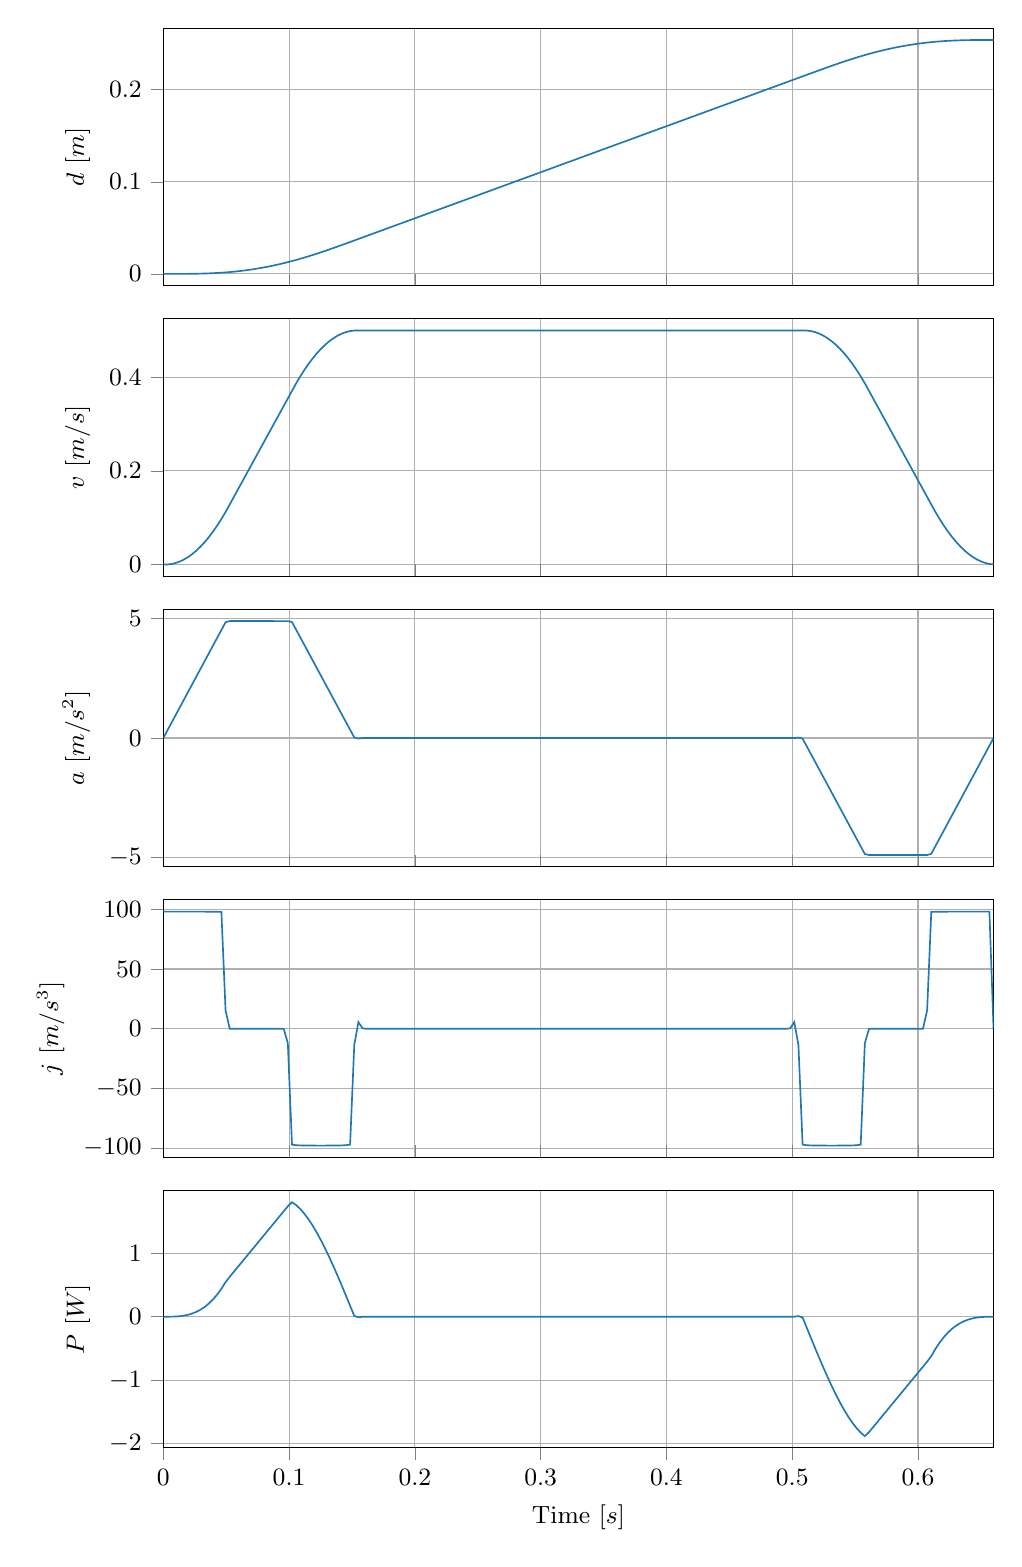
\begin{tikzpicture}

\definecolor{color0}{rgb}{0.12156862745098,0.466666666666667,0.705882352941177}

\begin{groupplot}[group style={group size=1 by 5,vertical sep=12}]
\nextgroupplot[
ytick align=outside,
xticklabels={},
tick pos=left,
x grid style={white!69.01960784313725!black},
xmajorgrids,
xmin=0, xmax=0.660065526635328,
y grid style={white!69.01960784313725!black},
%ylabel={Distance [$m$]},
ylabel={$d$ [$m$]},
ymajorgrids,
ymin=-0.0127, ymax=0.2667
%title = \footnotesize{Time}
]
\addplot [semithick, color0, forget plot]
table [row sep=\\]{%
0	0 \\
0.00330032763317664	1.9304767099347e-54 \\
0.00660065526635328	1.36450236350196e-38 \\
0.00990098289952992	3.52591962219528e-06 \\
0.0132013105327066	1.41036291372389e-05 \\
0.0165016381658832	3.5258941583591e-05 \\
0.0198019657990598	7.05176028306475e-05 \\
0.0231022934322365	0.000123405278886766 \\
0.0264026210654131	0.00019744753935727 \\
0.0297029486985898	0.000296169835339485 \\
0.0330032763317664	0.000423097468966021 \\
0.036303603964943	0.000581755549809146 \\
0.0396039315981197	0.000775668929357587 \\
0.0429042592312963	0.00100836209595871 \\
0.046204586864473	0.00128335899052278 \\
0.0495049144976496	0.00160418263678508 \\
0.0528052421308262	0.00197435421259847 \\
0.0561055697640029	0.00239738929957203 \\
0.0594058973971795	0.00287383924731233 \\
0.0627062250303562	0.00340370354613136 \\
0.0660065526635328	0.00398698162406344 \\
0.0693068802967094	0.00462367285041352 \\
0.0726072079298861	0.00531377652621804 \\
0.0759075355630627	0.00605729187252274 \\
0.0792078631962393	0.00685421801581524 \\
0.082508190829416	0.007704553969693 \\
0.0858085184625926	0.00860829861146637 \\
0.0891088460957693	0.00956545065181772 \\
0.0924091737289459	0.010576008594734 \\
0.0957095013621225	0.0116399706834759 \\
0.0990098289952992	0.0127573348259206 \\
0.102310156628476	0.0139280984883905 \\
0.105610484261652	0.0151522584774808 \\
0.108910811894829	0.0164293807740938 \\
0.112211139528006	0.0177559748978061 \\
0.115511467161182	0.019128533145679 \\
0.118811794794359	0.0205435423940555 \\
0.122112122427536	0.0219974869678191 \\
0.125412450060712	0.0234868497960351 \\
0.128712777693889	0.0250081130152648 \\
0.132013105327066	0.0265577583506249 \\
0.135313432960242	0.0281322674035955 \\
0.138613760593419	0.0297281219144619 \\
0.141914088226596	0.0313418040530982 \\
0.145214415859772	0.0329697968076074 \\
0.148514743492949	0.0346085846050359 \\
0.151815071126125	0.0362546545116954 \\
0.155115398759302	0.0379044992536054 \\
0.158415726392479	0.0395546299821568 \\
0.161716054025655	0.0412045512464358 \\
0.165016381658832	0.0428544619740113 \\
0.168316709292009	0.0445043744194074 \\
0.171617036925185	0.0461542869366769 \\
0.174917364558362	0.0478041994471601 \\
0.178217692191539	0.0494541119585764 \\
0.181518019824715	0.051104024470093 \\
0.184818347457892	0.0527539369816045 \\
0.188118675091068	0.0544038494931148 \\
0.191419002724245	0.0560537620046251 \\
0.194719330357422	0.0577036745161354 \\
0.198019657990598	0.0593535870276457 \\
0.201319985623775	0.0610034995391561 \\
0.204620313256952	0.0626534120506664 \\
0.207920640890128	0.0643033245621767 \\
0.211220968523305	0.0659532370736871 \\
0.214521296156482	0.0676031495851974 \\
0.217821623789658	0.0692530620967077 \\
0.221121951422835	0.0709029746082181 \\
0.224422279056012	0.0725528871197284 \\
0.227722606689188	0.0742027996312387 \\
0.231022934322365	0.0758527121427491 \\
0.234323261955541	0.0775026246542594 \\
0.237623589588718	0.0791525371657697 \\
0.240923917221895	0.0808024496772801 \\
0.244224244855071	0.0824523621887904 \\
0.247524572488248	0.0841022747003007 \\
0.250824900121425	0.085752187211811 \\
0.254125227754601	0.0874020997233214 \\
0.257425555387778	0.0890520122348317 \\
0.260725883020955	0.090701924746342 \\
0.264026210654131	0.0923518372578524 \\
0.267326538287308	0.0940017497693627 \\
0.270626865920484	0.095651662280873 \\
0.273927193553661	0.0973015747923834 \\
0.277227521186838	0.0989514873038937 \\
0.280527848820014	0.100601399815404 \\
0.283828176453191	0.102251312326914 \\
0.287128504086368	0.103901224838425 \\
0.290428831719544	0.105551137349935 \\
0.293729159352721	0.107201049861445 \\
0.297029486985898	0.108850962372956 \\
0.300329814619074	0.110500874884466 \\
0.303630142252251	0.112150787395976 \\
0.306930469885427	0.113800699907487 \\
0.310230797518604	0.115450612418997 \\
0.313531125151781	0.117100524930507 \\
0.316831452784957	0.118750437442018 \\
0.320131780418134	0.120400349953528 \\
0.323432108051311	0.122050262465038 \\
0.326732435684487	0.123700174976549 \\
0.330032763317664	0.125350087488059 \\
0.333333090950841	0.126999999999569 \\
0.336633418584017	0.12864991251108 \\
0.339933746217194	0.13029982502259 \\
0.343234073850371	0.1319497375341 \\
0.346534401483547	0.133599650045611 \\
0.349834729116724	0.135249562557121 \\
0.3531350567499	0.136899475068631 \\
0.356435384383077	0.138549387580142 \\
0.359735712016254	0.140199300091652 \\
0.36303603964943	0.141849212603162 \\
0.366336367282607	0.143499125114673 \\
0.369636694915784	0.145149037626183 \\
0.37293702254896	0.146798950137693 \\
0.376237350182137	0.148448862649204 \\
0.379537677815314	0.150098775160714 \\
0.38283800544849	0.151748687672224 \\
0.386138333081667	0.153398600183735 \\
0.389438660714843	0.155048512695245 \\
0.39273898834802	0.156698425206755 \\
0.396039315981197	0.158348337718266 \\
0.399339643614373	0.159998250229776 \\
0.40263997124755	0.161648162741286 \\
0.405940298880727	0.163298075252797 \\
0.409240626513903	0.164947987764307 \\
0.41254095414708	0.166597900275817 \\
0.415841281780257	0.168247812787328 \\
0.419141609413433	0.169897725298838 \\
0.42244193704661	0.171547637810348 \\
0.425742264679786	0.173197550321859 \\
0.429042592312963	0.174847462833369 \\
0.43234291994614	0.176497375344879 \\
0.435643247579316	0.17814728785639 \\
0.438943575212493	0.1797972003679 \\
0.44224390284567	0.18144711287941 \\
0.445544230478846	0.183097025390921 \\
0.448844558112023	0.184746937902431 \\
0.4521448857452	0.186396850413941 \\
0.455445213378376	0.188046762925452 \\
0.458745541011553	0.189696675436962 \\
0.46204586864473	0.191346587948472 \\
0.465346196277906	0.192996500459983 \\
0.468646523911083	0.194646412971493 \\
0.471946851544259	0.196296325483003 \\
0.475247179177436	0.197946237994514 \\
0.478547506810613	0.199596150506024 \\
0.481847834443789	0.201246063017534 \\
0.485148162076966	0.202895975529046 \\
0.488448489710143	0.204545888040563 \\
0.491748817343319	0.206195800551978 \\
0.495049144976496	0.207845713062427 \\
0.498349472609673	0.209495625579625 \\
0.501649800242849	0.211145538026112 \\
0.504950127876026	0.212795448753601 \\
0.508250455509202	0.214445370017843 \\
0.511550783142379	0.216095500746394 \\
0.514851110775556	0.217745345488304 \\
0.518151438408732	0.219391415394964 \\
0.521451766041909	0.221030203192392 \\
0.524752093675086	0.222658195946902 \\
0.528052421308262	0.224271878085538 \\
0.531352748941439	0.225867732596404 \\
0.534653076574616	0.227442241649375 \\
0.537953404207792	0.228991886984735 \\
0.541253731840969	0.230513150203965 \\
0.544554059474146	0.232002513032181 \\
0.547854387107322	0.233456457605944 \\
0.551154714740499	0.234871466854321 \\
0.554455042373675	0.236244025102194 \\
0.557755370006852	0.237570619225906 \\
0.561055697640029	0.238847741522519 \\
0.564356025273205	0.240071901511609 \\
0.567656352906382	0.241242665174079 \\
0.570956680539559	0.242360029316524 \\
0.574257008172735	0.243423991405266 \\
0.577557335805912	0.244434549348182 \\
0.580857663439089	0.245391701388534 \\
0.584157991072265	0.246295446030307 \\
0.587458318705442	0.247145781984185 \\
0.590758646338619	0.247942708127477 \\
0.594058973971795	0.248686223473782 \\
0.597359301604972	0.249376327149586 \\
0.600659629238148	0.250013018375937 \\
0.603959956871325	0.250596296453869 \\
0.607260284504502	0.251126160752688 \\
0.610560612137678	0.251602610700428 \\
0.613860939770855	0.252025645787401 \\
0.617161267404032	0.252395817363215 \\
0.620461595037208	0.252716641009477 \\
0.623761922670385	0.252991637904041 \\
0.627062250303562	0.253224331070642 \\
0.630362577936738	0.253418244450191 \\
0.633662905569915	0.253576902531034 \\
0.636963233203091	0.25370383016466 \\
0.640263560836268	0.253802552460643 \\
0.643563888469445	0.253876594721113 \\
0.646864216102621	0.253929482397169 \\
0.650164543735798	0.253964741058416 \\
0.653464871368975	0.253985896370863 \\
0.656765199002151	0.253996474080378 \\
0.660065526635328	0.254 \\
};
\nextgroupplot[
ytick align=outside,
xticklabels={},
tick pos=left,
x grid style={white!69.01960784313725!black},
xmajorgrids,
xmin=0, xmax=0.660065526635328,
y grid style={white!69.01960784313725!black},
%ylabel={Velocity [$m/s$]},
ylabel={$v$ [$m/s$]},
ymajorgrids,
ymin=-0.0249994987158772, ymax=0.524989473033422
]
\addplot [semithick, color0, forget plot]
table [row sep=\\]{%
0	5.8499027971765e-52 \\
0.00330032763317664	1.47012512924192e-56 \\
0.00660065526635328	0.00106835442237641 \\
0.00990098289952992	0.00320504831360106 \\
0.0132013105327066	0.00641006433230687 \\
0.0165016381658832	0.0106833821262526 \\
0.0198019657990598	0.0160249774975261 \\
0.0231022934322365	0.0224348212359867 \\
0.0264026210654131	0.0299128774336849 \\
0.0297029486985898	0.038459100954279 \\
0.0330032763317664	0.0480734334519435 \\
0.036303603964943	0.0587557967273079 \\
0.0396039315981197	0.0705060807484586 \\
0.0429042592312963	0.0833241196418378 \\
0.046204586864473	0.0972096355032201 \\
0.0495049144976496	0.112162069029823 \\
0.0528052421308262	0.128179724558555 \\
0.0561055697640029	0.144364439139552 \\
0.0594058973971795	0.160548999284967 \\
0.0627062250303562	0.176733386124656 \\
0.0660065526635328	0.192917581863611 \\
0.0693068802967094	0.209101565816449 \\
0.0726072079298861	0.225285313745974 \\
0.0759075355630627	0.241468797001057 \\
0.0792078631962393	0.257651981375952 \\
0.082508190829416	0.273834825575637 \\
0.0858085184625926	0.290017279111792 \\
0.0891088460957693	0.306199279355666 \\
0.0924091737289459	0.322380747307146 \\
0.0957095013621225	0.338561581344941 \\
0.0990098289952992	0.354741647677875 \\
0.102310156628476	0.370920746408472 \\
0.105610484261652	0.386968337256772 \\
0.108910811894829	0.401958311767816 \\
0.112211139528006	0.415885451515555 \\
0.115511467161182	0.428748114021207 \\
0.118811794794359	0.440545526191923 \\
0.122112122427536	0.451277265094584 \\
0.125412450060712	0.460943090600222 \\
0.128712777693889	0.469542878041028 \\
0.132013105327066	0.47707658995512 \\
0.135313432960242	0.483544268400529 \\
0.138613760593419	0.488946043542689 \\
0.141914088226596	0.493282163305169 \\
0.145214415859772	0.496553063688125 \\
0.148514743492949	0.498759544389579 \\
0.151815071126125	0.499903320302171 \\
0.155115398759302	0.499989974317544 \\
0.158415726392479	0.499926506596802 \\
0.161716054025655	0.499923313973345 \\
0.165016381658832	0.499923834473077 \\
0.168316709292009	0.499923856251023 \\
0.171617036925185	0.499923854194774 \\
0.174917364558362	0.499923854477508 \\
0.178217692191539	0.499923854507902 \\
0.181518019824715	0.499923854506346 \\
0.184818347457892	0.499923854505995 \\
0.188118675091068	0.499923854505997 \\
0.191419002724245	0.499923854506 \\
0.194719330357422	0.499923854506 \\
0.198019657990598	0.499923854506 \\
0.201319985623775	0.499923854506 \\
0.204620313256952	0.499923854506 \\
0.207920640890128	0.499923854506 \\
0.211220968523305	0.499923854506 \\
0.214521296156482	0.499923854506 \\
0.217821623789658	0.499923854506 \\
0.221121951422835	0.499923854506 \\
0.224422279056012	0.499923854506 \\
0.227722606689188	0.499923854506 \\
0.231022934322365	0.499923854506 \\
0.234323261955541	0.499923854506 \\
0.237623589588718	0.499923854506 \\
0.240923917221895	0.499923854506 \\
0.244224244855071	0.499923854506 \\
0.247524572488248	0.499923854506 \\
0.250824900121425	0.499923854506 \\
0.254125227754601	0.499923854506 \\
0.257425555387778	0.499923854506 \\
0.260725883020955	0.499923854506 \\
0.264026210654131	0.499923854506 \\
0.267326538287308	0.499923854506 \\
0.270626865920484	0.499923854506 \\
0.273927193553661	0.499923854506 \\
0.277227521186838	0.499923854506 \\
0.280527848820014	0.499923854506 \\
0.283828176453191	0.499923854506 \\
0.287128504086368	0.499923854506 \\
0.290428831719544	0.499923854506 \\
0.293729159352721	0.499923854506 \\
0.297029486985898	0.499923854506 \\
0.300329814619074	0.499923854506 \\
0.303630142252251	0.499923854506 \\
0.306930469885427	0.499923854506 \\
0.310230797518604	0.499923854506 \\
0.313531125151781	0.499923854506 \\
0.316831452784957	0.499923854506 \\
0.320131780418134	0.499923854506 \\
0.323432108051311	0.499923854506 \\
0.326732435684487	0.499923854506 \\
0.330032763317664	0.499923854506 \\
0.333333090950841	0.499923854506 \\
0.336633418584017	0.499923854506 \\
0.339933746217194	0.499923854506 \\
0.343234073850371	0.499923854506 \\
0.346534401483547	0.499923854506 \\
0.349834729116724	0.499923854506 \\
0.3531350567499	0.499923854506 \\
0.356435384383077	0.499923854506 \\
0.359735712016254	0.499923854506 \\
0.36303603964943	0.499923854506 \\
0.366336367282607	0.499923854506 \\
0.369636694915784	0.499923854506 \\
0.37293702254896	0.499923854506 \\
0.376237350182137	0.499923854506 \\
0.379537677815314	0.499923854506 \\
0.38283800544849	0.499923854506 \\
0.386138333081667	0.499923854506 \\
0.389438660714843	0.499923854506 \\
0.39273898834802	0.499923854506 \\
0.396039315981197	0.499923854506 \\
0.399339643614373	0.499923854506 \\
0.40263997124755	0.499923854506 \\
0.405940298880727	0.499923854506 \\
0.409240626513903	0.499923854506 \\
0.41254095414708	0.499923854506 \\
0.415841281780257	0.499923854506 \\
0.419141609413433	0.499923854506 \\
0.42244193704661	0.499923854506 \\
0.425742264679786	0.499923854506 \\
0.429042592312963	0.499923854506 \\
0.43234291994614	0.499923854506 \\
0.435643247579316	0.499923854506 \\
0.438943575212493	0.499923854506 \\
0.44224390284567	0.499923854506 \\
0.445544230478846	0.499923854506 \\
0.448844558112023	0.499923854506 \\
0.4521448857452	0.499923854506 \\
0.455445213378376	0.499923854506 \\
0.458745541011553	0.499923854506 \\
0.46204586864473	0.499923854506 \\
0.465346196277906	0.499923854506 \\
0.468646523911083	0.499923854506 \\
0.471946851544259	0.499923854506 \\
0.475247179177436	0.499923854505997 \\
0.478547506810613	0.499923854505995 \\
0.481847834443789	0.499923854506351 \\
0.485148162076966	0.499923854507994 \\
0.488448489710143	0.499923854477324 \\
0.491748817343319	0.499923854184437 \\
0.495049144976496	0.499923856229178 \\
0.498349472609673	0.499923834803654 \\
0.501649800242849	0.499923313947033 \\
0.504950127876026	0.499926506585708 \\
0.508250455509202	0.499989974317542 \\
0.511550783142379	0.499903320302173 \\
0.514851110775556	0.498759544389582 \\
0.518151438408732	0.496553063688129 \\
0.521451766041909	0.493282163305173 \\
0.524752093675086	0.488946043542693 \\
0.528052421308262	0.483544268400533 \\
0.531352748941439	0.477076589955124 \\
0.534653076574616	0.469542878041032 \\
0.537953404207792	0.460943090600226 \\
0.541253731840969	0.451277265094588 \\
0.544554059474146	0.440545526191926 \\
0.547854387107322	0.42874811402121 \\
0.551154714740499	0.415885451515557 \\
0.554455042373675	0.401958311767818 \\
0.557755370006852	0.386968337256774 \\
0.561055697640029	0.370920746408473 \\
0.564356025273205	0.354741647677875 \\
0.567656352906382	0.338561581344942 \\
0.570956680539559	0.322380747307147 \\
0.574257008172735	0.306199279355667 \\
0.577557335805912	0.290017279111793 \\
0.580857663439089	0.273834825575638 \\
0.584157991072265	0.257651981375952 \\
0.587458318705442	0.241468797001057 \\
0.590758646338619	0.225285313745974 \\
0.594058973971795	0.209101565816449 \\
0.597359301604972	0.192917581863611 \\
0.600659629238148	0.176733386124656 \\
0.603959956871325	0.160548999284967 \\
0.607260284504502	0.144364439139553 \\
0.610560612137678	0.128179724558555 \\
0.613860939770855	0.112162069029823 \\
0.617161267404032	0.0972096355032202 \\
0.620461595037208	0.0833241196418379 \\
0.623761922670385	0.0705060807484587 \\
0.627062250303562	0.0587557967273079 \\
0.630362577936738	0.0480734334519435 \\
0.633662905569915	0.038459100954279 \\
0.636963233203091	0.0299128774336849 \\
0.640263560836268	0.0224348212359867 \\
0.643563888469445	0.0160249774975261 \\
0.646864216102621	0.0106833821262526 \\
0.650164543735798	0.00641006433230687 \\
0.653464871368975	0.00320504831360106 \\
0.656765199002151	0.00106835442237641 \\
0.660065526635328	2.29799021682434e-51 \\
};
\nextgroupplot[
ytick align=outside,
xticklabels={},
tick pos=left,
x grid style={white!69.01960784313725!black},
xmajorgrids,
xmin=0, xmax=0.660065526635328,
y grid style={white!69.01960784313725!black},
%ylabel={Acceleration [$m/s^2$]},
ylabel={$a$ [$m/s^2$]},
ymajorgrids,
ymin=-5.39436929234858, ymax=5.39436929234858
]
\addplot [semithick, color0, forget plot]
table [row sep=\\]{%
0	0 \\
0.00330032763317664	0.323711625366145 \\
0.00660065526635328	0.647418719809963 \\
0.00990098289952992	0.971120559815732 \\
0.0132013105327066	1.29481623308793 \\
0.0165016381658832	1.6185045743874 \\
0.0198019657990598	1.94218406500781 \\
0.0231022934322365	2.26585267551164 \\
0.0264026210654131	2.58950760969395 \\
0.0297029486985898	2.91314486507831 \\
0.0330032763317664	3.23675842603615 \\
0.036303603964943	3.56033864729998 \\
0.0396039315981197	3.88386860883918 \\
0.0429042592312963	4.2073143653369 \\
0.046204586864473	4.53059065296832 \\
0.0495049144976496	4.85335315430917 \\
0.0528052421308262	4.90397208395325 \\
0.0561055697640029	4.90392528993755 \\
0.0594058973971795	4.90387277826455 \\
0.0627062250303562	4.90381487469993 \\
0.0660065526635328	4.90375070345978 \\
0.0693068802967094	4.90367918834407 \\
0.0726072079298861	4.90359899192969 \\
0.0759075355630627	4.90350843116711 \\
0.0792078631962393	4.90340535800355 \\
0.082508190829416	4.90328698686764 \\
0.0858085184625926	4.90314963920674 \\
0.0891088460957693	4.902988354494 \\
0.0924091737289459	4.90279627850782 \\
0.0957095013621225	4.90256366376574 \\
0.0990098289952992	4.90227048004462 \\
0.102310156628476	4.86242356273508 \\
0.105610484261652	4.54196557952487 \\
0.108910811894829	4.2199264120735 \\
0.112211139528006	3.89738957318954 \\
0.115511467161182	3.57461848700138 \\
0.118811794794359	3.25171925198584 \\
0.122112122427536	2.92874725783927 \\
0.125412450060712	2.60573748931942 \\
0.128712777693889	2.28271636984123 \\
0.132013105327066	1.95970799395559 \\
0.135313432960242	1.63673905822481 \\
0.138613760593419	1.31384524339077 \\
0.141914088226596	0.991083536699343 \\
0.145214415859772	0.66856413868501 \\
0.148514743492949	0.346564353518824 \\
0.151815071126125	0.0262561857500026 \\
0.155115398759302	-0.0192307333771689 \\
0.158415726392479	-0.000967365599965547 \\
0.161716054025655	0.000157711435318978 \\
0.165016381658832	6.5988206306752e-06 \\
0.168316709292009	-6.230463491966e-07 \\
0.171617036925185	8.5668462946096e-08 \\
0.174917364558362	9.20959977828398e-09 \\
0.178217692191539	-4.7159510096632e-10 \\
0.181518019824715	-1.06180363453087e-10 \\
0.184818347457892	4.77918538745403e-13 \\
0.188118675091068	1.04401565693984e-12 \\
0.191419002724245	3.53609541170004e-14 \\
0.194719330357422	-1.06170109124987e-14 \\
0.198019657990598	-5.49564726011714e-15 \\
0.201319985623775	6.03873025703199e-15 \\
0.204620313256952	1.49822779465689e-15 \\
0.207920640890128	-6.45236194758753e-15 \\
0.211220968523305	2.09348667934519e-15 \\
0.214521296156482	-3.85407038429761e-15 \\
0.217821623789658	-4.02733761336132e-16 \\
0.221121951422835	-7.86522937921989e-16 \\
0.224422279056012	7.7649503408089e-15 \\
0.227722606689188	7.02463875708386e-16 \\
0.231022934322365	8.89876766839045e-16 \\
0.234323261955541	-4.55272394763277e-15 \\
0.237623589588718	9.6031233171621e-16 \\
0.240923917221895	7.27394219605992e-16 \\
0.244224244855071	-3.12617990978548e-15 \\
0.247524572488248	5.53422670958592e-15 \\
0.250824900121425	-1.50474064216173e-15 \\
0.254125227754601	-4.28041190644812e-15 \\
0.257425555387778	-1.73263183295305e-15 \\
0.260725883020955	-1.50263146925097e-15 \\
0.264026210654131	1.01519342043858e-16 \\
0.267326538287308	-5.17742757648415e-15 \\
0.270626865920484	-2.30845564499204e-15 \\
0.273927193553661	1.55867657683676e-15 \\
0.277227521186838	1.74661694742636e-15 \\
0.280527848820014	7.66211649871023e-15 \\
0.283828176453191	3.3979919651668e-15 \\
0.287128504086368	4.53112337015998e-15 \\
0.290428831719544	8.07102748405055e-15 \\
0.293729159352721	8.00425275654289e-15 \\
0.297029486985898	-2.63010635933099e-15 \\
0.300329814619074	-5.92584103496117e-17 \\
0.303630142252251	-4.83330079360465e-15 \\
0.306930469885427	-4.99928848901137e-15 \\
0.310230797518604	6.69287671832599e-15 \\
0.313531125151781	-6.17260357685337e-15 \\
0.316831452784957	-3.65568535859468e-15 \\
0.320131780418134	2.73735024184671e-15 \\
0.323432108051311	3.48413205980004e-15 \\
0.326732435684487	-1.04563061588001e-15 \\
0.330032763317664	-4.53748383332274e-15 \\
0.333333090950841	-1.79144325779794e-15 \\
0.336633418584017	6.18555188958279e-15 \\
0.339933746217194	-1.230589852617e-15 \\
0.343234073850371	-9.18523723545373e-16 \\
0.346534401483547	6.56707220137881e-15 \\
0.349834729116724	-1.70620056840614e-15 \\
0.3531350567499	1.88233693079122e-15 \\
0.356435384383077	-1.64668590781016e-15 \\
0.359735712016254	-5.88516480413747e-15 \\
0.36303603964943	3.69299811265528e-15 \\
0.366336367282607	-4.5544561124753e-15 \\
0.369636694915784	7.27215449096717e-15 \\
0.37293702254896	-6.31885244366754e-15 \\
0.376237350182137	5.97356567621306e-15 \\
0.379537677815314	6.54243621082012e-15 \\
0.38283800544849	4.47346241280137e-15 \\
0.386138333081667	4.80675951434611e-15 \\
0.389438660714843	-1.92169880900555e-15 \\
0.39273898834802	-6.01121865448001e-16 \\
0.396039315981197	6.64726097433787e-15 \\
0.399339643614373	3.87180464981395e-15 \\
0.40263997124755	7.81629037775261e-15 \\
0.405940298880727	3.60989792738888e-15 \\
0.409240626513903	-6.3297150177979e-15 \\
0.41254095414708	-8.1832103392123e-15 \\
0.415841281780257	-7.81929929277498e-15 \\
0.419141609413433	-7.89854197125933e-15 \\
0.42244193704661	2.66241413057503e-15 \\
0.425742264679786	-4.87575261995347e-15 \\
0.429042592312963	6.64670106534389e-16 \\
0.43234291994614	-1.67439532084167e-15 \\
0.435643247579316	7.06257869338571e-15 \\
0.438943575212493	1.35784076231216e-15 \\
0.44224390284567	6.51957889676548e-15 \\
0.445544230478846	1.3473295212673e-15 \\
0.448844558112023	-5.6986038641228e-15 \\
0.4521448857452	-5.96917669773545e-15 \\
0.455445213378376	-4.63144598501049e-15 \\
0.458745541011553	4.13595281416347e-15 \\
0.46204586864473	5.45950181638641e-15 \\
0.465346196277906	8.22553924471345e-15 \\
0.468646523911083	-3.29559698070538e-14 \\
0.471946851544259	-1.05838009516032e-12 \\
0.475247179177436	-6.73433900597358e-13 \\
0.478547506810613	1.07994244429196e-10 \\
0.481847834443789	4.9792455857962e-10 \\
0.485148162076966	-9.29327882895179e-09 \\
0.488448489710143	-8.87447092172379e-08 \\
0.491748817343319	6.19559473423544e-07 \\
0.495049144976496	-6.49203758309579e-06 \\
0.498349472609673	-0.000157819571883665 \\
0.501649800242849	0.000967370211010038 \\
0.504950127876026	0.0192307367379679 \\
0.508250455509202	-0.026256185748913 \\
0.511550783142379	-0.34656435351847 \\
0.514851110775556	-0.668564138684834 \\
0.518151438408732	-0.99108353669925 \\
0.521451766041909	-1.31384524339073 \\
0.524752093675086	-1.6367390582248 \\
0.528052421308262	-1.9597079939556 \\
0.531352748941439	-2.28271636984127 \\
0.534653076574616	-2.60573748931948 \\
0.537953404207792	-2.92874725783934 \\
0.541253731840969	-3.25171925198593 \\
0.544554059474146	-3.57461848700148 \\
0.547854387107322	-3.89738957318965 \\
0.551154714740499	-4.21992641207364 \\
0.554455042373675	-4.54196557952503 \\
0.557755370006852	-4.86242356273531 \\
0.561055697640029	-4.90227048004465 \\
0.564356025273205	-4.90256366376576 \\
0.567656352906382	-4.90279627850784 \\
0.570956680539559	-4.90298835449402 \\
0.574257008172735	-4.90314963920676 \\
0.577557335805912	-4.90328698686766 \\
0.580857663439089	-4.90340535800356 \\
0.584157991072265	-4.90350843116712 \\
0.587458318705442	-4.9035989919297 \\
0.590758646338619	-4.90367918834408 \\
0.594058973971795	-4.90375070345979 \\
0.597359301604972	-4.90381487469993 \\
0.600659629238148	-4.90387277826455 \\
0.603959956871325	-4.90392528993755 \\
0.607260284504502	-4.90397208395326 \\
0.610560612137678	-4.85335315430918 \\
0.613860939770855	-4.53059065296833 \\
0.617161267404032	-4.2073143653369 \\
0.620461595037208	-3.88386860883918 \\
0.623761922670385	-3.56033864729998 \\
0.627062250303562	-3.23675842603615 \\
0.630362577936738	-2.91314486507831 \\
0.633662905569915	-2.58950760969395 \\
0.636963233203091	-2.26585267551164 \\
0.640263560836268	-1.94218406500781 \\
0.643563888469445	-1.6185045743874 \\
0.646864216102621	-1.29481623308793 \\
0.650164543735798	-0.971120559815733 \\
0.653464871368975	-0.647418719809964 \\
0.656765199002151	-0.323711625366145 \\
0.660065526635328	0 \\
};
\nextgroupplot[
ytick align=outside,
xticklabels={},
tick pos=left,
x grid style={white!69.01960784313725!black},
xmajorgrids,
xmin=0, xmax=0.660065526635328,
y grid style={white!69.01960784313725!black},
%ylabel={Jerk [$m/s^3$]},
ylabel={$j$ [$m/s^3$]},
ymajorgrids,
ymin=-107.673478580786, ymax=107.882702016969
]
\addplot [semithick, color0, forget plot]
table [row sep=\\]{%
0	98.0846938079797 \\
0.00330032763317664	98.0833209375163 \\
0.00660065526635328	98.0817288416298 \\
0.00990098289952992	98.0798603199999 \\
0.0132013105327066	98.0776387306454 \\
0.0165016381658832	98.0749569729415 \\
0.0198019657990598	98.0716602952212 \\
0.0231022934322365	98.0675163667869 \\
0.0264026210654131	98.062159687113 \\
0.0297029486985898	98.0549802706585 \\
0.0330032763317664	98.0448783360254 \\
0.036303603964943	98.0296496283911 \\
0.0396039315981197	98.004135482268 \\
0.0429042592312963	97.9527863784446 \\
0.046204586864473	97.7971090192 \\
0.0495049144976496	15.337546834804 \\
0.0528052421308262	-0.0141785970684603 \\
0.0561055697640029	-0.0159110484894104 \\
0.0594058973971795	-0.0175447928377748 \\
0.0627062250303562	-0.0194438999018947 \\
0.0660065526635328	-0.0216690958171342 \\
0.0693068802967094	-0.0242995312275456 \\
0.0726072079298861	-0.0274399310127994 \\
0.0759075355630627	-0.031231191269297 \\
0.0792078631962393	-0.0358664802599279 \\
0.082508190829416	-0.0416163715143896 \\
0.0858085184625926	-0.0488693034953776 \\
0.0891088460957693	-0.0581990661335532 \\
0.0924091737289459	-0.0704823181002615 \\
0.0957095013621225	-0.0888347320942743 \\
0.0990098289952992	-12.0736247237712 \\
0.102310156628476	-97.0988395182482 \\
0.105610484261652	-97.5779386913192 \\
0.108910811894829	-97.7287332450396 \\
0.112211139528006	-97.7997102298213 \\
0.115511467161182	-97.838539352752 \\
0.118811794794359	-97.8605853854888 \\
0.122112122427536	-97.8720310289117 \\
0.125412450060712	-97.8754703717918 \\
0.128712777693889	-97.8716090604422 \\
0.132013105327066	-97.8596586848298 \\
0.135313432960242	-97.8368970365643 \\
0.138613760593419	-97.7968682402474 \\
0.141914088226596	-97.7234486577009 \\
0.145214415859772	-97.566005850229 \\
0.148514743492949	-97.0534454061278 \\
0.151815071126125	-13.7825465200194 \\
0.155115398759302	5.53380446629458 \\
0.158415726392479	0.340898556448411 \\
0.161716054025655	-0.0457870959516916 \\
0.165016381658832	-0.00218825781431192 \\
0.168316709292009	0.00021474150200455 \\
0.171617036925185	-2.3167037384652e-05 \\
0.174917364558362	-2.93343273226787e-06 \\
0.178217692191539	1.10719411152853e-07 \\
0.181518019824715	3.23175105766984e-08 \\
0.184818347457892	1.71513205979636e-10 \\
0.188118675091068	-3.05604978744475e-10 \\
0.191419002724245	-1.39171390326557e-11 \\
0.194719330357422	1.55016323197182e-12 \\
0.198019657990598	3.49047334731682e-12 \\
0.201319985623775	-1.37821268002293e-12 \\
0.204620313256952	-2.40946496020785e-12 \\
0.207920640890128	2.58999612039398e-12 \\
0.211220968523305	-1.80137930768341e-12 \\
0.214521296156482	1.04619402773296e-12 \\
0.217821623789658	-1.16159996681405e-13 \\
0.221121951422835	2.59105009740704e-12 \\
0.224422279056012	-2.14004046169988e-12 \\
0.227722606689188	5.66869465502817e-14 \\
0.231022934322365	-1.64918132544232e-12 \\
0.234323261955541	1.67040535061477e-12 \\
0.237623589588718	-7.06017533811197e-14 \\
0.240923917221895	-1.16764895144288e-12 \\
0.244224244855071	2.62409910585134e-12 \\
0.247524572488248	-2.13280864387257e-12 \\
0.250824900121425	-8.41023825559425e-13 \\
0.254125227754601	7.71987483720802e-13 \\
0.257425555387778	6.9702919815072e-14 \\
0.260725883020955	4.86073581813011e-13 \\
0.264026210654131	-1.59950572949037e-12 \\
0.267326538287308	8.69316256215639e-13 \\
0.270626865920484	1.17175864832111e-12 \\
0.273927193553661	5.69615241838577e-14 \\
0.277227521186838	1.79241160055365e-12 \\
0.280527848820014	-1.29201870653551e-12 \\
0.283828176453191	3.43348626360588e-13 \\
0.287128504086368	1.0725996949754e-12 \\
0.290428831719544	-2.02271852461794e-14 \\
0.293729159352721	-3.22220954949017e-12 \\
0.297029486985898	7.78969867537238e-13 \\
0.300329814619074	-1.44653508700258e-12 \\
0.303630142252251	-5.02939013299562e-14 \\
0.306930469885427	3.54272820604856e-12 \\
0.310230797518604	-3.89824492621264e-12 \\
0.313531125151781	7.62625565453897e-13 \\
0.316831452784957	1.93708959876616e-12 \\
0.320131780418134	2.26273064015003e-13 \\
0.323432108051311	-1.3725210795784e-12 \\
0.326732435684487	-1.05803428576997e-12 \\
0.330032763317664	8.32048910003737e-13 \\
0.333333090950841	2.41702967673834e-12 \\
0.336633418584017	-2.24709495543426e-12 \\
0.339933746217194	9.45545111227831e-14 \\
0.343234073850371	2.26813600015407e-12 \\
0.346534401483547	-2.50680504109294e-12 \\
0.349834729116724	1.08732723613121e-12 \\
0.3531350567499	-1.06929469301584e-12 \\
0.356435384383077	-1.2842588310304e-12 \\
0.359735712016254	2.90218783736044e-12 \\
0.36303603964943	-2.49897682311132e-12 \\
0.366336367282607	3.58347155212623e-12 \\
0.369636694915784	-4.11807047924187e-12 \\
0.37293702254896	3.72461532802351e-12 \\
0.376237350182137	1.72379864056345e-13 \\
0.379537677815314	-6.26885964440463e-13 \\
0.38283800544849	1.01004626627664e-13 \\
0.386138333081667	-2.03870800549285e-12 \\
0.389438660714843	4.00152238554007e-13 \\
0.39273898834802	2.19627871997616e-12 \\
0.396039315981197	-8.40948718652576e-13 \\
0.399339643614373	1.19519278604313e-12 \\
0.40263997124755	-1.2745282727256e-12 \\
0.405940298880727	-3.01169972324387e-12 \\
0.409240626513903	-5.61609498128864e-13 \\
0.41254095414708	1.10258742170492e-13 \\
0.415841281780257	-2.40252945781517e-14 \\
0.419141609413433	3.19994488413858e-12 \\
0.42244193704661	-2.28411279810171e-12 \\
0.425742264679786	1.67867755697423e-12 \\
0.429042592312963	-7.08836504623307e-13 \\
0.43234291994614	2.64719989883532e-12 \\
0.435643247579316	-1.72858539362915e-12 \\
0.438943575212493	1.56413596695393e-12 \\
0.44224390284567	-1.56675440762344e-12 \\
0.445544230478846	-2.1341875939654e-12 \\
0.448844558112023	-8.1381902146289e-14 \\
0.4521448857452	4.04898574757909e-13 \\
0.455445213378376	2.65408471431176e-12 \\
0.458745541011553	3.96590079593828e-13 \\
0.46204586864473	8.36498071154078e-13 \\
0.465346196277906	-1.24638141792647e-11 \\
0.468646523911083	-3.10686101412271e-10 \\
0.471946851544259	1.16624545721424e-10 \\
0.475247179177436	3.29263567123623e-08 \\
0.478547506810613	1.18147621169681e-07 \\
0.481847834443789	-2.96676527456634e-06 \\
0.485148162076966	-2.40737844748467e-05 \\
0.488448489710143	0.000214617081646938 \\
0.491748817343319	-0.00215484620042855 \\
0.495049144976496	-0.0458522162496914 \\
0.498349472609673	0.340932718794001 \\
0.501649800242849	5.53380408748144 \\
0.504950127876026	-13.7825475380154 \\
0.508250455509202	-97.0534454063505 \\
0.511550783142379	-97.5660058502831 \\
0.514851110775556	-97.7234486577259 \\
0.518151438408732	-97.7968682402624 \\
0.521451766041909	-97.8368970365747 \\
0.524752093675086	-97.8596586848376 \\
0.528052421308262	-97.8716090604486 \\
0.531352748941439	-97.8754703717973 \\
0.534653076574616	-97.8720310289166 \\
0.537953404207792	-97.8605853854934 \\
0.541253731840969	-97.8385393527566 \\
0.544554059474146	-97.7997102298261 \\
0.547854387107322	-97.728733245045 \\
0.551154714740499	-97.5779386913264 \\
0.554455042373675	-97.098839518272 \\
0.557755370006852	-12.0736247237091 \\
0.561055697640029	-0.0888347320923705 \\
0.564356025273205	-0.0704823180988865 \\
0.567656352906382	-0.0581990661325026 \\
0.570956680539559	-0.0488693034945457 \\
0.574257008172735	-0.0416163715137052 \\
0.577557335805912	-0.0358664802592628 \\
0.580857663439089	-0.0312311912686647 \\
0.584157991072265	-0.0274399310124121 \\
0.587458318705442	-0.0242995312273087 \\
0.590758646338619	-0.0216690958169337 \\
0.594058973971795	-0.019443899901657 \\
0.597359301604972	-0.0175447928377465 \\
0.600659629238148	-0.0159110484893193 \\
0.603959956871325	-0.0141785970681221 \\
0.607260284504502	15.3375468348017 \\
0.610560612137678	97.7971090192012 \\
0.613860939770855	97.9527863784452 \\
0.617161267404032	98.0041354822684 \\
0.620461595037208	98.0296496283914 \\
0.623761922670385	98.0448783360256 \\
0.627062250303562	98.0549802706587 \\
0.630362577936738	98.0621596871132 \\
0.633662905569915	98.067516366787 \\
0.636963233203091	98.0716602952213 \\
0.640263560836268	98.0749569729416 \\
0.643563888469445	98.0776387306455 \\
0.646864216102621	98.07986032 \\
0.650164543735798	98.0817288416299 \\
0.653464871368975	98.0833209375164 \\
0.656765199002151	98.0846938079798 \\
0.660065526635328	0 \\
};
\nextgroupplot[
tick align=outside,
tick pos=left,
x grid style={white!69.01960784313725!black},
xlabel={Time [$s$]},
xmajorgrids,
xmin=0, xmax=0.660065526635328,
y grid style={white!69.01960784313725!black},
%ylabel={Power [$W$]},
ylabel={$P$ [$W$]},
ymajorgrids,
ymin=-2.06586284802753, ymax=1.98783266416152
]
\addplot [semithick, color0, forget plot]
table [row sep=\\]{%
0	0 \\
0.00330032763317664	4.75896595078515e-57 \\
0.00660065526635328	0.000691672652438246 \\
0.00990098289952992	0.00311248831254073 \\
0.0132013105327066	0.0082998553526089 \\
0.0165016381658832	0.0172911028412684 \\
0.0198019657990598	0.0311234559378039 \\
0.0231022934322365	0.0508339997221857 \\
0.0264026210654131	0.0774596237423694 \\
0.0297029486985898	0.112036932460486 \\
0.0330032763317664	0.155602090794066 \\
0.036303603964943	0.209190533841136 \\
0.0396039315981197	0.273836353751219 \\
0.0429042592312963	0.350570765548154 \\
0.046204586864473	0.440417065989347 \\
0.0495049144976496	0.544362131519735 \\
0.0528052421308262	0.628589790963969 \\
0.0561055697640029	0.707952424064101 \\
0.0594058973971795	0.787311867171164 \\
0.0627062250303562	0.866667807734175 \\
0.0660065526635328	0.946019727773443 \\
0.0693068802967094	1.02536699654428 \\
0.0726072079298861	1.10470883738132 \\
0.0759075355630627	1.18404428195846 \\
0.0792078631962393	1.26337210597907 \\
0.082508190829416	1.34269073679619 \\
0.0858085184625926	1.42199811744071 \\
0.0891088460957693	1.50129150083529 \\
0.0924091737289459	1.58056712816004 \\
0.0957095013621225	1.65981970664878 \\
0.0990098289952992	1.73903950745364 \\
0.102310156628476	1.80357377724384 \\
0.105610484261652	1.75759686818623 \\
0.108910811894829	1.69623449638148 \\
0.112211139528006	1.62086762237795 \\
0.115511467161182	1.53261093464718 \\
0.118811794794359	1.43253036889451 \\
0.122112122427536	1.32167705267097 \\
0.125412450060712	1.20109669161976 \\
0.128712777693889	1.07183321404662 \\
0.132013105327066	0.934930807064121 \\
0.135313432960242	0.791435790471886 \\
0.138613760593419	0.642399433583299 \\
0.141914088226596	0.48888383099919 \\
0.145214415859772	0.331977571336054 \\
0.148514743492949	0.172852279062718 \\
0.151815071126125	0.0131255544348969 \\
0.155115398759302	-0.00961517388735825 \\
0.158415726392479	-0.000483611704992695 \\
0.161716054025655	7.8843623396156e-05 \\
0.165016381658832	3.29890771268719e-06 \\
0.168316709292009	-3.11475733513486e-07 \\
0.171617036925185	4.28277081789545e-08 \\
0.174917364558362	4.60409861935493e-09 \\
0.178217692191539	-2.35761640642126e-10 \\
0.181518019824715	-5.30820965703519e-11 \\
0.184818347457892	2.38922878029475e-13 \\
0.188118675091068	5.21928331381975e-13 \\
0.191419002724245	1.76777844811807e-14 \\
0.194719330357422	-5.30769701870864e-15 \\
0.198019657990598	-2.7474051612831e-15 \\
0.201319985623775	3.01890530641744e-15 \\
0.204620313256952	7.48999814032897e-16 \\
0.207920640890128	-3.2256896555058e-15 \\
0.211220968523305	1.04658393009521e-15 \\
0.214521296156482	-1.92674172205548e-15 \\
0.217821623789658	-2.01336214306859e-16 \\
0.221121951422835	-3.93201578783344e-16 \\
0.224422279056012	3.88188390442487e-15 \\
0.227722606689188	3.5117844839536e-16 \\
0.231022934322365	4.44870623313513e-16 \\
0.234323261955541	-2.27601530440235e-15 \\
0.237623589588718	4.80083042401212e-16 \\
0.240923917221895	3.63641722010811e-16 \\
0.244224244855071	-1.56285191037918e-15 \\
0.247524572488248	2.76669194836625e-15 \\
0.250824900121425	-7.52255741861326e-16 \\
0.254125227754601	-2.13988001914492e-15 \\
0.257425555387778	-8.66183984369686e-16 \\
0.260725883020955	-7.51201316009962e-16 \\
0.264026210654131	5.07519407814787e-17 \\
0.267326538287308	-2.58831955046162e-15 \\
0.270626865920484	-1.15405204400055e-15 \\
0.273927193553661	7.79219602220451e-16 \\
0.277227521186838	8.7317547670289e-16 \\
0.280527848820014	3.83047481370924e-15 \\
0.283828176453191	1.69873724080661e-15 \\
0.287128504086368	2.2652166604526e-15 \\
0.290428831719544	4.03489916965042e-15 \\
0.293729159352721	4.0015168904912e-15 \\
0.297029486985898	-1.31485290891749e-15 \\
0.300329814619074	-2.96246929138761e-17 \\
0.303630142252251	-2.41628236272575e-15 \\
0.306930469885427	-2.49926357121404e-15 \\
0.310230797518604	3.345928726759e-15 \\
0.313531125151781	-3.08583177247806e-15 \\
0.316831452784957	-1.8275643153298e-15 \\
0.320131780418134	1.36846668403694e-15 \\
0.323432108051311	1.74180072894317e-15 \\
0.326732435684487	-5.22735687880219e-16 \\
0.330032763317664	-2.26839640771337e-15 \\
0.333333090950841	-8.95585218567131e-16 \\
0.336633418584017	3.0923049428871e-15 \\
0.339933746217194	-6.1520122243626e-16 \\
0.343234073850371	-4.59191920330007e-16 \\
0.346534401483547	3.2830360477325e-15 \\
0.349834729116724	-8.52970364717927e-16 \\
0.3531350567499	9.41025133920139e-16 \\
0.356435384383077	-8.23217566193166e-16 \\
0.359735712016254	-2.94213427328745e-15 \\
0.36303603964943	1.84621785116201e-15 \\
0.366336367282607	-2.27688125492707e-15 \\
0.369636694915784	3.63552350368743e-15 \\
0.37293702254896	-3.15894506969293e-15 \\
0.376237350182137	2.98632797799718e-15 \\
0.379537677815314	3.27071992837282e-15 \\
0.38283800544849	2.23639057239537e-15 \\
0.386138333081667	2.4030137440953e-15 \\
0.389438660714843	-9.60703075797645e-16 \\
0.39273898834802	-3.00515160002602e-16 \\
0.396039315981197	3.3231243281983e-15 \\
0.399339643614373	1.93560750442924e-15 \\
0.40263997124755	3.90755001358424e-15 \\
0.405940298880727	1.80467408623347e-15 \\
0.409240626513903	-3.16437552962205e-15 \\
0.41254095414708	-4.09098205501237e-15 \\
0.415841281780257	-3.90905424198011e-15 \\
0.419141609413433	-3.94866954724939e-15 \\
0.42244193704661	1.33100433444831e-15 \\
0.425742264679786	-2.43750504338487e-15 \\
0.429042592312963	3.32284441633586e-16 \\
0.43234291994614	-8.37070162761981e-16 \\
0.435643247579316	3.53075156314934e-15 \\
0.438943575212493	6.78816987700458e-16 \\
0.44224390284567	3.25929301182698e-15 \\
0.445544230478846	6.73562167561675e-16 \\
0.448844558112023	-2.84886800905506e-15 \\
0.4521448857452	-2.98413382295931e-15 \\
0.455445213378376	-2.31537032876278e-15 \\
0.458745541011553	2.06766147291154e-15 \\
0.46204586864473	2.72933519173041e-15 \\
0.465346196277906	4.11214328460752e-15 \\
0.468646523911083	-1.64754754549257e-14 \\
0.471946851544259	-5.29109456704975e-13 \\
0.475247179177436	-3.36665671341639e-13 \\
0.478547506810613	5.39888989395061e-11 \\
0.481847834443789	2.48924364578497e-10 \\
0.485148162076966	-4.64593177318712e-09 \\
0.488448489710143	-4.43655970963508e-08 \\
0.491748817343319	3.09732559850379e-07 \\
0.495049144976496	-3.245524463326e-06 \\
0.498349472609673	-7.88977655831525e-05 \\
0.501649800242849	0.000483610921701779 \\
0.504950127876026	0.00961395503648173 \\
0.508250455509202	-0.0131278296382756 \\
0.511550783142379	-0.173248671022259 \\
0.514851110775556	-0.333452745205661 \\
0.518151438408732	-0.492125566518878 \\
0.521451766041909	-0.64809642390799 \\
0.524752093675086	-0.800277086830807 \\
0.528052421308262	-0.94760556821594 \\
0.531352748941439	-1.08903054155861 \\
0.534653076574616	-1.22350548015448 \\
0.537953404207792	-1.3499858126154 \\
0.541253731840969	-1.46742697089163 \\
0.544554059474146	-1.57478218229145 \\
0.547854387107322	-1.67099842911099 \\
0.551154714740499	-1.75500600124767 \\
0.554455042373675	-1.82568081645342 \\
0.557755370006852	-1.88160396110984 \\
0.561055697640029	-1.81835382555439 \\
0.564356025273205	-1.73914351192995 \\
0.567656352906382	-1.65989846106371 \\
0.570956680539559	-1.58062904976002 \\
0.574257008172735	-1.50134088609811 \\
0.577557335805912	-1.42203795063562 \\
0.580857663439089	-1.34272315093555 \\
0.584157991072265	-1.2633986629839 \\
0.587458318705442	-1.18406614955686 \\
0.590758646338619	-1.1047269044557 \\
0.594058973971795	-1.02538195046696 \\
0.597359301604972	-0.946032107533919 \\
0.600659629238148	-0.866678041227221 \\
0.603959956871325	-0.787320297867717 \\
0.607260284504502	-0.707959179455935 \\
0.610560612137678	-0.622101470504744 \\
0.613860939770855	-0.508160421564106 \\
0.617161267404032	-0.408991495901863 \\
0.620461595037208	-0.323619932636095 \\
0.623761922670385	-0.251025524158391 \\
0.627062250303562	-0.190178320135581 \\
0.630362577936738	-0.140044875807213 \\
0.633662905569915	-0.0995901345830933 \\
0.636963233203091	-0.0677781733653667 \\
0.640263560836268	-0.0435725523058321 \\
0.643563888469445	-0.0259364993842012 \\
0.646864216102621	-0.0138330166013534 \\
0.650164543735798	-0.00622494526284471 \\
0.653464871368975	-0.00207500827612068 \\
0.656765199002151	-0.000345838746534576 \\
0.660065526635328	0 \\
};
\end{groupplot}

\end{tikzpicture}
\par\end{centering}
\caption{Minimum time trajectory}

\centering{}\label{fig:min_t}
\end{figure}


\subsection{Total Energy and Peak Power Comparison}

The generated trajectory profiles for the various optimization problems
considered will naturally exhibit different total energy and peak
power consumption characteristics that may further aid in the selection
of the proper trajectory. A relative comparison of these values for
the above cases is provided in Tables \ref{tab:energy} and \ref{tab:power}.
The total energy was found via trapezoidal integration of the absolute
value of the power. The results were divided by the best case over
all combinations. It can be seen that, in general, minimizing the
velocity resulted in the lowest energy required for the move, which
makes sense as kinetic energy is proportional to the velocity squared.
As expected per previous discussion, the minimization of the $\mathcal{L}_{1}$
norm of Power similarly achieves the minimum total energy mark. Minimal
peak power, on the other hand, is generally reduced by minimizing
the jerk or more directly so by minimizing the $\mathcal{L}_{\infty}$
norm of the power. Simultaneous comparison of these tables illustrates
the well-known tradeoff that must be considered between system specifications
and performance requirements.

\begin{table}
\caption{Total energy relative to best case}
\label{tab:energy}
\centering{}%
\begin{tabular}{|l|c|c|c|c|c|c|}
\hline 
 & $v$ & $a$ & $j$ & $P$ & $E_{total}$ & $t_{f}$\tabularnewline
\hline 
$\|\cdot\|_{1}$ & 1.17 & 1.00 & 3.08 & 1.00 & \multirow{3}{*}{1.00} & \multirow{3}{*}{3.08}\tabularnewline
\cline{1-5} \cline{2-5} \cline{3-5} \cline{4-5} \cline{5-5} 
$\|\cdot\|_{2}$ & 1.17 & 1.85 & 2.80 & 1.39 &  & \tabularnewline
\cline{1-5} \cline{2-5} \cline{3-5} \cline{4-5} \cline{5-5} 
$\|\cdot\|_{\infty}$ & 1.00 & 3.08 & 3.08 & 1.96 &  & \tabularnewline
\hline 
\end{tabular}
\end{table}

\begin{table}
\caption{Peak power relative to best case}
\label{tab:power}
\centering{}%
\begin{tabular}{|l|c|c|c|c|c|c|}
\hline 
 & $v$ & $a$ & $j$ & $P$ & $E_{total}$ & $t_{f}$\tabularnewline
\hline 
$\|\cdot\|_{1}$ & 2.37 & 5.13 & 3.06 & 5.13 & \multirow{3}{*}{5.13} & \multirow{3}{*}{11.2}\tabularnewline
\cline{1-5} \cline{2-5} \cline{3-5} \cline{4-5} \cline{5-5} 
$\|\cdot\|_{2}$ & 5.45 & 1.41 & 2.59 & 1.77 &  & \tabularnewline
\cline{1-5} \cline{2-5} \cline{3-5} \cline{4-5} \cline{5-5} 
$\|\cdot\|_{\infty}$ & 5.13 & 3.06 & 3.33 & 1.00 &  & \tabularnewline
\hline 
\end{tabular}
\end{table}


\subsection{Multi-Objective Trajectory Optimization}

Extension of the trajectory optimization framework to mixed optimization
problems can be easily handled by modifying the cost function in \eqref{eq:baseProgram}
with the weighted multi-objective formulation

\begin{align}
\begin{split} & \min\limits _{\mathbf{x}}\;\sum_{i}w_{i}J_{i}\\
s.t.\quad & \mathcal{C}\\
 & \sum_{i}w_{i}=1
\end{split}
\label{eq:multioptStatement}
\end{align}
where $w_{i}$ are weights for each of the $J_{i}$ cost functions.
Equal weighting of total energy and peak power cost functions results
in the motion profiles shown in Fig. \ref{fig:multiobj_e_p}, which
exhibits a total energy 1.50 times greater and peak power 1.08 times
greater than their respective optimal cases. Varying the cost function
weights provides a means to extracting the multi-objective Pareto
front, as shown in Fig. \ref{fig:pareto} in which weights were varied
from 0 to 1. Representing the range of possible solutions to this
problem, at the extremes the Pareto front replicates the best and
worst energy and power case results shown in Tables \ref{tab:energy}
and \ref{tab:power}. In between lies a trade space between the two
cost functions where an engineer can find a motion profile that appropriately
balances the needs of their particular system.

\begin{figure}
\centering{}% This file was created by tikzplotlib v0.9.8.
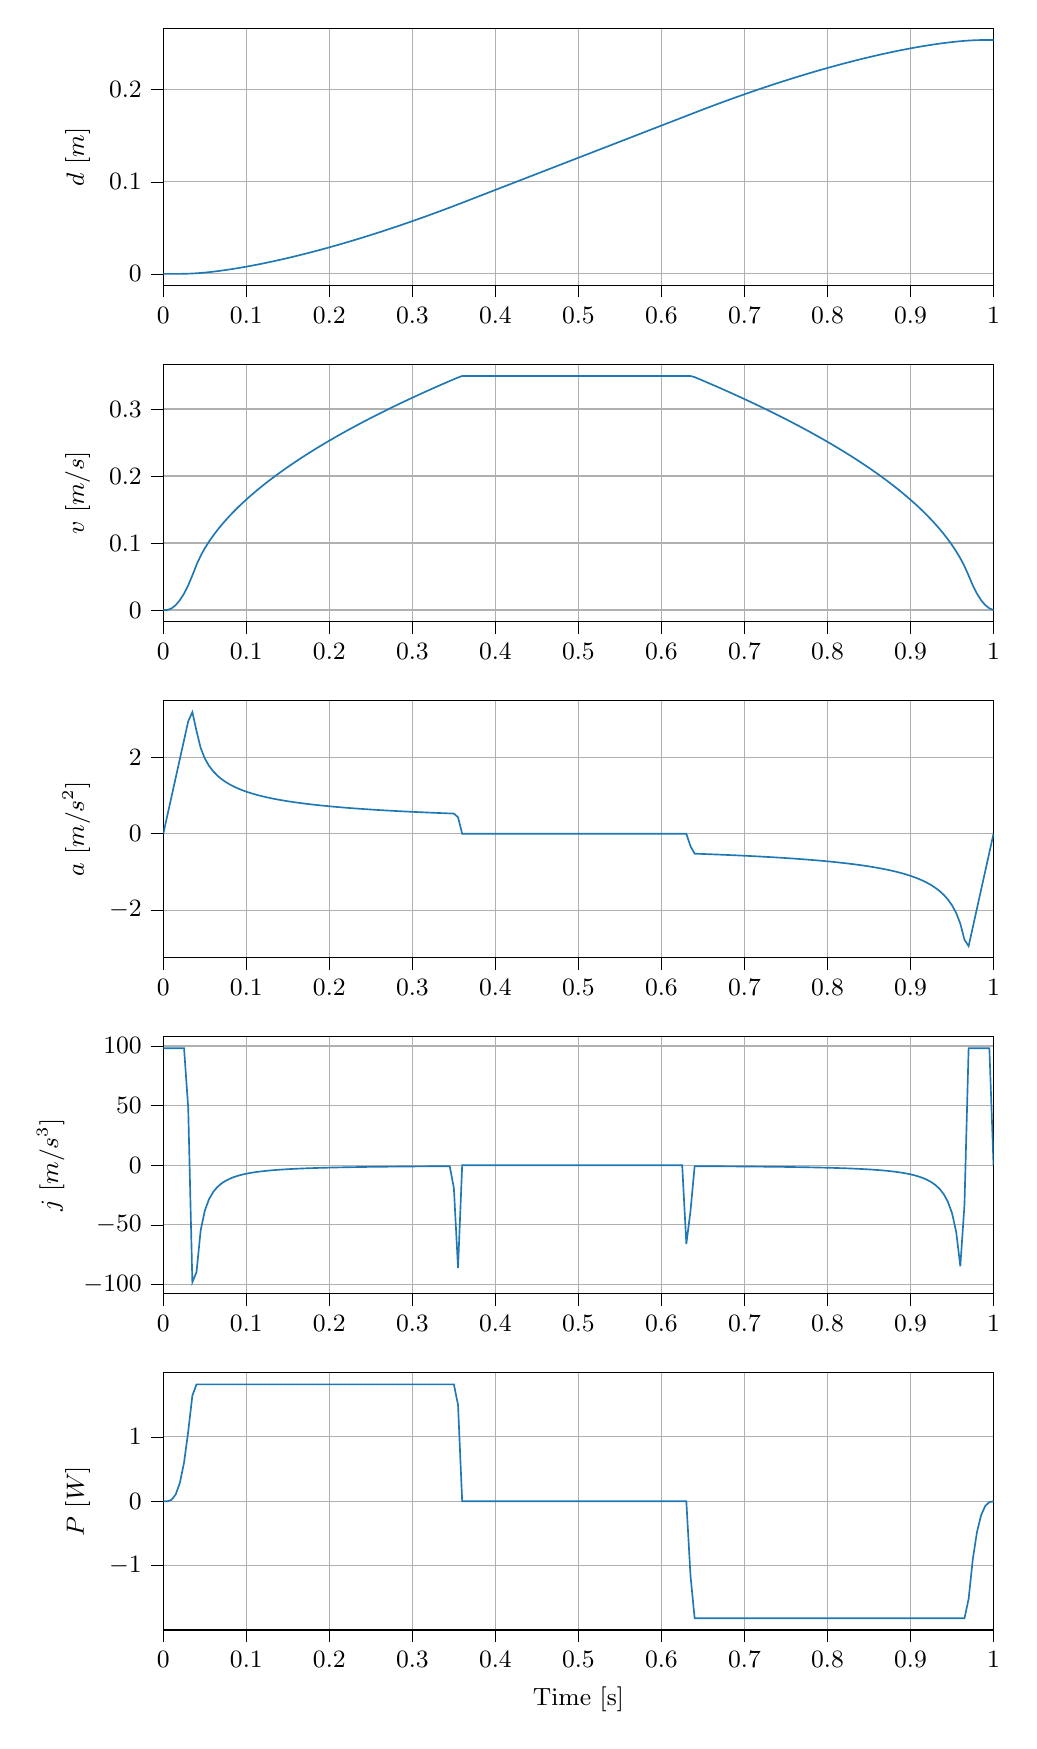
\begin{tikzpicture}

\definecolor{color0}{rgb}{0.12156862745098,0.466666666666667,0.705882352941177}

\begin{groupplot}[group style={group size=1 by 5}]
\nextgroupplot[
tick align=outside,
tick pos=left,
%title={Minimum Mixed Objective},
x grid style={white!69.0196078431373!black},
xmajorgrids,
xmin=0, xmax=1,
xtick style={color=black},
y grid style={white!69.0196078431373!black},
%ylabel={Distance [$m$]},
ylabel={$d$ [$m$]},
ymajorgrids,
ymin=-0.0127, ymax=0.2667,
ytick style={color=black}
]
\addplot [semithick, color0]
table {%
0 0
0.005 1.68807185859196e-39
0.01 4.86476736674278e-39
0.015 1.22624983908442e-05
0.02 4.90499931729681e-05
0.025 0.000122624981758809
0.03 0.000245249960577419
0.035 0.00042918742408564
0.04 0.000686699860812089
0.045 0.00102380833069699
0.05 0.00142825034584902
0.055 0.00188881587096085
0.06 0.00239866581669289
0.065 0.00295303612552734
0.07 0.00354835145617467
0.075 0.004181795662243
0.08 0.0048510736537654
0.085 0.0055542668550625
0.09 0.00628973952541833
0.095 0.00705607493724717
0.1 0.00785203015032001
0.105 0.00867650292556987
0.11 0.00952850687304129
0.115 0.0104071523656795
0.12 0.0113116316007226
0.125 0.0122412067142633
0.13 0.0131952001887407
0.135 0.0141729870128478
0.14 0.0151739882016336
0.145 0.0161976653869956
0.15 0.0172435162609539
0.155 0.0183110707059304
0.16 0.0193998874840764
0.165 0.0205095513857154
0.17 0.0216396707579978
0.175 0.0227898753508572
0.18 0.0239598144296451
0.185 0.0251491551133713
0.19 0.0263575809049609
0.195 0.0275847903858664
0.2 0.0288304960520967
0.205 0.0300944232725266
0.21 0.031376309353426
0.215 0.032675902695656
0.22 0.0339929620330379
0.225 0.0353272557420986
0.23 0.0366785612148023
0.235 0.0380466642870594
0.24 0.0394313587167826
0.245 0.0408324457060946
0.25 0.0422497334629922
0.255 0.0436830367983684
0.26 0.0451321767548028
0.265 0.0465969802639674
0.27 0.0480772798298684
0.275 0.0495729132354678
0.28 0.0510837232705073
0.285 0.0526095574786019
0.29 0.0541502679218775
0.295 0.055705710961614
0.3 0.0572757470535141
0.305 0.0588602405563594
0.31 0.0604590595529347
0.315 0.0620720756822118
0.32 0.0636991639818669
0.325 0.0653402027402817
0.33 0.0669950733572182
0.335 0.0686636602123598
0.34 0.0703458505408047
0.345 0.0720415343141952
0.35 0.0737506041247144
0.355 0.0754729550625355
0.36 0.0772084845254729
0.365 0.0789548011616216
0.37 0.0807011179655414
0.375 0.0824474348582539
0.38 0.0841937518105269
0.385 0.0859400688071023
0.39 0.08768638583859
0.395 0.0894327028986149
0.4 0.0911790199825537
0.405 0.0929253370868912
0.41 0.094671654208856
0.415 0.0964179713462002
0.42 0.0981642884970573
0.425 0.099910605659847
0.43 0.101656922833209
0.435 0.103403240015953
0.44 0.105149557207029
0.445 0.106895874405492
0.45 0.10864219161049
0.455 0.110388508821241
0.46 0.112134826037025
0.465 0.11388114325717
0.47 0.115627460481044
0.475 0.117373777708049
0.48 0.119120094937613
0.485 0.120866412169185
0.49 0.122612729402231
0.495 0.124359046636226
0.5 0.126105363870656
0.505 0.127851681105008
0.51 0.129597998338769
0.515 0.131344315571421
0.52 0.133090632802437
0.525 0.134836950031279
0.53 0.13658326725739
0.535 0.13832958448019
0.54 0.140075901699072
0.545 0.141822218913393
0.55 0.143568536122466
0.555 0.145314853325554
0.56 0.147061170521856
0.565 0.148807487710492
0.57 0.150553804890489
0.575 0.152300122060756
0.58 0.154046439220056
0.585 0.155792756366966
0.59 0.157539073499828
0.595 0.159285390616669
0.6 0.161031707715101
0.605 0.162778024792153
0.61 0.16452434184402
0.615 0.16627065886563
0.62 0.168016975849865
0.625 0.169763292785972
0.63 0.17150960965575
0.635 0.173255926421586
0.64 0.175002242959304
0.645 0.176740304602208
0.65 0.17846530689874
0.655 0.180177150750876
0.66 0.181875734940047
0.665 0.183560955921008
0.67 0.185232707706501
0.675 0.186890881761585
0.68 0.188535366896474
0.685 0.190166049154869
0.69 0.191782811696466
0.695 0.193385534672796
0.7 0.194974095095715
0.705 0.196548366697842
0.71 0.198108219784277
0.715 0.199653521074817
0.72 0.201184133535873
0.725 0.202699916201196
0.73 0.204200723980409
0.735 0.205686407454272
0.74 0.20715681265546
0.745 0.208611780833513
0.75 0.210051148202446
0.755 0.211474745669363
0.76 0.212882398542164
0.765 0.214273926214259
0.77 0.215649141823897
0.775 0.217007851885426
0.78 0.21834985588944
0.785 0.219674945868368
0.79 0.220982905923563
0.795 0.222273511709396
0.8 0.223546529869217
0.805 0.224801717417236
0.81 0.226038821059509
0.815 0.227257576446077
0.82 0.228457707345051
0.825 0.229638924727861
0.83 0.230800925753007
0.835 0.231943392633397
0.84 0.233065991369582
0.845 0.234168370327789
0.85 0.235250158637485
0.855 0.236310964377962
0.86 0.237350372516941
0.865 0.238367942555902
0.87 0.239363205826376
0.875 0.2403356623679
0.88 0.241284777300801
0.885 0.242209976583925
0.89 0.243110642016803
0.895 0.243986105304526
0.9 0.244835640947312
0.905 0.245658457638672
0.91 0.246453687745927
0.915 0.247220374288333
0.92 0.247957454595141
0.925 0.248663739475106
0.93 0.24933788618595
0.935 0.24997836262473
0.94 0.25058339872249
0.945 0.251150918540277
0.95 0.251678442038726
0.955 0.25216293673534
0.96 0.252600581168288
0.965 0.252986359970697
0.97 0.253313300121329
0.975 0.253570812565845
0.98 0.253754750034065
0.985 0.253877375015712
0.99 0.253950950005863
0.995 0.253987737501378
1 0.254
};

\nextgroupplot[
tick align=outside,
tick pos=left,
x grid style={white!69.0196078431373!black},
xmajorgrids,
xmin=0, xmax=1,
xtick style={color=black},
y grid style={white!69.0196078431373!black},
%ylabel={Velocity [$m/s$]},
ylabel={$v$ [$m/s$]},
ymajorgrids,
ymin=-0.0174631723443006, ymax=0.366726619230313,
ytick style={color=black}
]
\addplot [semithick, color0]
table {%
0 3.37614372417057e-37
0.005 2.59892684000837e-37
0.01 0.00245249967816884
0.015 0.00735749895642478
0.02 0.0147149977171683
0.025 0.0245249957637218
0.03 0.0367874927016443
0.035 0.0515024873452897
0.04 0.0674216939769804
0.045 0.0808884030304052
0.05 0.0921131050223669
0.055 0.101969989146407
0.06 0.11087406176689
0.065 0.119063066129467
0.07 0.126688841213666
0.075 0.13385559830448
0.08 0.140638640259421
0.085 0.147094534071165
0.09 0.153267082365769
0.095 0.159191042614567
0.1 0.164894555049972
0.105 0.170400789494283
0.11 0.175729098527634
0.115 0.18089584700863
0.12 0.185915022708147
0.125 0.190798694895469
0.13 0.195557364821415
0.135 0.20020023775717
0.14 0.204735437072389
0.145 0.209170174791673
0.15 0.213510888995297
0.155 0.217763355629207
0.16 0.221932780327793
0.165 0.226023874456481
0.17 0.230040918571872
0.175 0.233987815757587
0.18 0.237868136745237
0.185 0.24168515831792
0.19 0.245441896181095
0.195 0.249141133246061
0.2 0.252785444085992
0.205 0.256377216179877
0.21 0.259918668445987
0.215 0.263411867476395
0.22 0.266858741812127
0.225 0.270261094540741
0.23 0.27362061445142
0.235 0.276938885944637
0.24 0.280217397862403
0.245 0.283457551379531
0.25 0.286660667075236
0.255 0.289827991286869
0.26 0.292960701832919
0.265 0.296059913180214
0.27 0.299126681119873
0.275 0.302162007007906
0.28 0.305166841618922
0.285 0.308142088655115
0.29 0.311088607947291
0.295 0.314007218380035
0.3 0.316898700569048
0.305 0.319763799315065
0.31 0.322603225855415
0.315 0.325417659931032
0.32 0.328207751682958
0.325 0.330974123387288
0.33 0.333717371028335
0.335 0.336438065688976
0.34 0.339136754678094
0.345 0.341813962103836
0.35 0.344470187564231
0.355 0.347105892587473
0.36 0.349263327229748
0.365 0.349263360783951
0.37 0.349263378542511
0.375 0.349263390454597
0.38 0.349263399315071
0.385 0.349263406297552
0.39 0.349263412004964
0.395 0.349263416787766
0.4 0.349263420867495
0.405 0.349263424392966
0.41 0.349263427468842
0.415 0.34926343017142
0.42 0.349263432557934
0.425 0.349263434672316
0.43 0.349263436548928
0.435 0.349263438215064
0.44 0.349263439692667
0.445 0.349263440999549
0.45 0.349263442150274
0.455 0.349263443156799
0.46 0.349263444028959
0.465 0.34926344477483
0.47 0.349263445401005
0.475 0.349263445912803
0.48 0.349263446314433
0.485 0.34926344660911
0.49 0.349263446799147
0.495 0.349263446886013
0.5 0.349263446870375
0.505 0.349263446752114
0.51 0.349263446530321
0.515 0.349263446203272
0.52 0.349263445768388
0.525 0.349263445222161
0.53 0.349263444560058
0.535 0.349263443776389
0.54 0.349263442864133
0.545 0.349263441814712
0.55 0.349263440617683
0.555 0.349263439260353
0.56 0.349263437727244
0.565 0.349263435999388
0.57 0.349263434053356
0.575 0.34926343185991
0.58 0.349263429382075
0.585 0.349263426572327
0.59 0.349263423368348
0.595 0.349263419686389
0.6 0.349263415410399
0.605 0.349263410373254
0.61 0.349263404321968
0.615 0.349263396847171
0.62 0.349263387221421
0.625 0.349263373955547
0.63 0.349263353167174
0.635 0.349263307543573
0.64 0.347612328580737
0.645 0.34500045930653
0.65 0.342368770427182
0.655 0.339716837834119
0.66 0.33704419619217
0.665 0.334350357098749
0.67 0.331634811016759
0.675 0.328897026977696
0.68 0.326136451679025
0.685 0.32335250831935
0.69 0.320544595266158
0.695 0.317712084583682
0.7 0.314854320425505
0.705 0.311970617287015
0.71 0.309060258107854
0.715 0.30612249221127
0.72 0.303156533064604
0.725 0.300161555842604
0.73 0.297136694772612
0.735 0.294081040237683
0.74 0.290993635610453
0.745 0.28787347378672
0.75 0.28471949338336
0.755 0.28153057456014
0.76 0.278305534419018
0.765 0.275043121927662
0.77 0.27174201230572
0.775 0.26840080080279
0.78 0.265017995785671
0.785 0.26159201103893
0.79 0.25812115716668
0.795 0.254603631964098
0.8 0.251037509603875
0.805 0.247420728454577
0.81 0.243751077313534
0.815 0.240026179794921
0.82 0.236243476562046
0.825 0.232400205029077
0.83 0.228493376077976
0.835 0.224519747236988
0.84 0.220475791641544
0.845 0.216357661939114
0.85 0.212161148095406
0.855 0.20788162779577
0.86 0.203514007792255
0.865 0.199052654094854
0.87 0.194491308304817
0.875 0.189822986580203
0.88 0.185039856624748
0.885 0.180133086575523
0.89 0.175092657544625
0.895 0.16990712855722
0.9 0.164563338272057
0.905 0.159046021450993
0.91 0.153337308481224
0.915 0.147416061361502
0.92 0.141256975992918
0.925 0.134829342168913
0.93 0.128095287755952
0.935 0.121007219552057
0.94 0.113503963557329
0.945 0.105504699689861
0.95 0.0968989393228647
0.955 0.0875288865894994
0.96 0.0771557604818095
0.965 0.0653880301264388
0.97 0.051502488903184
0.975 0.0367874936440142
0.98 0.0245249963293189
0.985 0.0147149980303518
0.99 0.0073574991029834
0.995 0.00245249972431613
1 0
};

\nextgroupplot[
tick align=outside,
tick pos=left,
x grid style={white!69.0196078431373!black},
xmajorgrids,
xmin=0, xmax=1,
xtick style={color=black},
y grid style={white!69.0196078431373!black},
%ylabel={Acceleration [$m/s^2$]},
ylabel={$a$ [$m/s^2$]},
ymajorgrids,
ymin=-3.24934107074255, ymax=3.49018334524675,
ytick style={color=black}
]
\addplot [semithick, color0]
table {%
0 3.49320243338249e-35
0.005 0.490499935633769
0.01 0.980999855651188
0.015 1.47149975214869
0.02 1.96199960931071
0.025 2.4524993875845
0.03 2.94299892872907
0.035 3.18384132633815
0.04 2.69334181068497
0.045 2.24494039839234
0.05 1.97137682480807
0.055 1.78081452409658
0.06 1.63780087251531
0.065 1.5251550168398
0.07 1.43335141816285
0.075 1.35660839098814
0.08 1.29117876234888
0.085 1.23450965892083
0.09 1.18479204975959
0.095 1.14070248708104
0.1 1.1012468888622
0.105 1.06566180667005
0.11 1.0333496961992
0.115 1.0038351399035
0.12 0.976734437464321
0.125 0.951733985189269
0.13 0.928574587150964
0.135 0.907039863043894
0.14 0.886947543856754
0.145 0.86814284072485
0.15 0.850493326781967
0.155 0.833884939717129
0.16 0.818218825737692
0.165 0.803408823078093
0.17 0.789379437143053
0.175 0.77606419752994
0.18 0.76340431453672
0.185 0.751347572635
0.19 0.739847412993105
0.195 0.728862167986253
0.2 0.718354418776979
0.205 0.708290453222014
0.21 0.698639806081634
0.215 0.689374867146307
0.22 0.68047054572288
0.225 0.671903982135805
0.23 0.663654298643403
0.235 0.655702383553218
0.24 0.648030703425499
0.245 0.64062313914109
0.25 0.633464842326459
0.255 0.626542109210111
0.26 0.619842269458947
0.265 0.613353587931746
0.27 0.607065177606646
0.275 0.600966922203307
0.28 0.595049407238631
0.285 0.589303858435092
0.29 0.583722086548727
0.295 0.578296437802768
0.3 0.573019749203278
0.305 0.567885308070016
0.31 0.562886815123382
0.315 0.558018350385169
0.32 0.553274340866035
0.325 0.548649528209505
0.33 0.544138932128148
0.335 0.539737797823674
0.34 0.535441485148278
0.345 0.531245092079125
0.35 0.527141004648277
0.355 0.431486928454975
0.36 6.71084063226892e-06
0.365 3.55171201959153e-06
0.37 2.38241722333096e-06
0.375 1.77209479087405e-06
0.38 1.39649623125239e-06
0.385 1.14148230315077e-06
0.39 9.56560354762641e-07
0.395 8.15945925386273e-07
0.4 7.05094173873434e-07
0.405 6.15175120806951e-07
0.41 5.40515733125338e-07
0.415 4.77302755350586e-07
0.42 4.22876321742727e-07
0.425 3.75322551709576e-07
0.43 3.33227182040384e-07
0.435 2.95520523836516e-07
0.44 2.61376505385388e-07
0.445 2.30144952819482e-07
0.45 2.01304956416905e-07
0.455 1.74431986007731e-07
0.46 1.49174186684199e-07
0.465 1.25234929219301e-07
0.47 1.02359693236601e-07
0.475 8.0325989413837e-08
0.48 5.89354284359455e-08
0.485 3.80073049907574e-08
0.49 1.73732357202291e-08
0.495 -3.12749863117864e-09
0.5 -2.36521859875102e-08
0.505 -4.43587286788514e-08
0.51 -6.5409722517947e-08
0.515 -8.69767927208193e-08
0.52 -1.0924543457101e-07
0.525 -1.32420655978085e-07
0.53 -1.56733800685656e-07
0.535 -1.8245105790048e-07
0.54 -2.09884358218932e-07
0.545 -2.39405652669862e-07
0.55 -2.71466031071888e-07
0.555 -3.06621859031809e-07
0.56 -3.45571276362043e-07
0.565 -3.89206320335458e-07
0.57 -4.38689202950792e-07
0.575 -4.95567015268478e-07
0.58 -5.6194963385958e-07
0.585 -6.40795686190331e-07
0.59 -7.36391896379244e-07
0.595 -8.55197887696541e-07
0.6 -1.00742896832759e-06
0.605 -1.21025734389283e-06
0.61 -1.4949592592422e-06
0.615 -1.92515007665445e-06
0.62 -2.6531748075634e-06
0.625 -4.15767450384445e-06
0.63 -9.12472035999615e-06
0.635 -0.330195792567176
0.64 -0.522373854841325
0.645 -0.52633777586964
0.65 -0.530386518612593
0.655 -0.534528328389859
0.66 -0.538767818684107
0.665 -0.543109216398013
0.67 -0.547556807812657
0.675 -0.552115059734167
0.68 -0.556788671935069
0.685 -0.561582610638304
0.69 -0.566502136495152
0.695 -0.571552831635388
0.7 -0.576740627698117
0.705 -0.58207183583222
0.71 -0.587553179316731
0.715 -0.593191829333319
0.72 -0.598995444399846
0.725 -0.604972213998544
0.73 -0.611130906985795
0.735 -0.617480925445894
0.74 -0.624032364746717
0.745 -0.630796080671831
0.75 -0.637783764644115
0.755 -0.645008028224438
0.76 -0.652482498271079
0.765 -0.660221924388402
0.77 -0.668242300586024
0.775 -0.676561003423823
0.78 -0.685196949348232
0.785 -0.694170774449962
0.79 -0.703505040516466
0.795 -0.713224472044574
0.8 -0.723356229859624
0.805 -0.733930228208445
0.81 -0.744979503722648
0.815 -0.756540646574961
0.82 -0.768654306593882
0.825 -0.781365790220112
0.83 -0.794725768197772
0.835 -0.808791119088817
0.84 -0.823625940485872
0.845 -0.839302768741711
0.85 -0.855904059927066
0.855 -0.873524000703148
0.86 -0.892270739480207
0.865 -0.912269158007234
0.87 -0.93366434492289
0.875 -0.956625991091054
0.88 -0.981354009844913
0.885 -1.00808580617951
0.89 -1.03710579748114
0.895 -1.06875805703251
0.9 -1.10346336421281
0.905 -1.14174259395382
0.91 -1.18424942394447
0.915 -1.23181707371677
0.92 -1.28552676480093
0.925 -1.34681088259233
0.93 -1.41761364077883
0.935 -1.50065119894565
0.94 -1.59985277349358
0.945 -1.72115207339933
0.95 -1.87401054667306
0.955 -2.07462522153798
0.96 -2.35354607107415
0.965 -2.77710824465095
0.97 -2.94299905183395
0.975 -2.45249946293907
0.98 -1.96199965979343
0.985 -1.47149978547367
0.99 -0.980999875733455
0.995 -0.490499944863226
1 1.74372094396703e-36
};

\nextgroupplot[
tick align=outside,
tick pos=left,
x grid style={white!69.0196078431373!black},
xmajorgrids,
xmin=0, xmax=1,
xtick style={color=black},
y grid style={white!69.0196078431373!black},
%ylabel={Jerk [$m/s^3$]},
ylabel={$j$ [$m/s^3$]},
ymajorgrids,
ymin=-107.909897735799, ymax=107.909983577809,
ytick style={color=black}
]
\addplot [semithick, color0]
table {%
0 98.0999871267538
0.005 98.0999840034838
0.01 98.0999792995013
0.015 98.0999714324039
0.02 98.0999556547575
0.025 98.099908228913
0.03 48.168479521816
0.035 -98.0999031306354
0.04 -89.6802824585265
0.045 -54.7127147168535
0.05 -38.1124601422982
0.055 -28.6027303162535
0.06 -22.5291711351026
0.065 -18.3607197353889
0.07 -15.3486054349424
0.075 -13.0859257278528
0.08 -11.3338206856104
0.085 -9.94352183224647
0.09 -8.81791253571032
0.095 -7.89111964376803
0.1 -7.11701643843085
0.105 -6.46242209416895
0.11 -5.902911259141
0.115 -5.4201404878353
0.12 -5.00009045501028
0.125 -4.63187960766103
0.13 -4.3069448214141
0.135 -4.01846383742783
0.14 -3.76094062638094
0.145 -3.52990278857647
0.15 -3.32167741296766
0.155 -3.13322279588737
0.16 -2.96200053191977
0.165 -2.8058771870081
0.17 -2.66304792262253
0.175 -2.53197659864408
0.18 -2.41134838034389
0.185 -2.30003192837914
0.19 -2.19704900137041
0.195 -2.10154984185475
0.2 -2.01279311099305
0.205 -1.93012942807587
0.21 -1.85298778706538
0.215 -1.78086428468555
0.22 -1.71331271741491
0.225 -1.64993669848039
0.23 -1.59038301803702
0.235 -1.53433602554379
0.24 -1.48151285688175
0.245 -1.43165936292619
0.25 -1.38454662326962
0.255 -1.3399679502329
0.26 -1.29773630544015
0.265 -1.2576820650201
0.27 -1.21965108066767
0.275 -1.18350299293529
0.28 -1.14910976070775
0.285 -1.11635437727293
0.29 -1.0851297491919
0.295 -1.05533771989793
0.3 -1.02688822665241
0.305 -0.999698589326772
0.31 -0.973692947642598
0.315 -0.948801903826957
0.32 -0.924962531305847
0.325 -0.902119216271402
0.33 -0.880226860894808
0.335 -0.859262535079304
0.34 -0.83927861383056
0.345 -0.820817486169602
0.35 -19.1308152386604
0.355 -86.2960435228686
0.36 -0.000631825722535478
0.365 -0.000233858959252113
0.37 -0.000122064486491383
0.375 -7.51197119243309e-05
0.38 -5.10027856203243e-05
0.385 -3.69843896776258e-05
0.39 -2.81228858752736e-05
0.395 -2.21703503025677e-05
0.4 -1.79838106132965e-05
0.405 -1.49318775363226e-05
0.41 -1.26425955549505e-05
0.415 -1.08852867215718e-05
0.42 -9.51075400663018e-06
0.425 -8.41907393383825e-06
0.43 -7.54133164077366e-06
0.435 -6.82880369022562e-06
0.44 -6.24631051318127e-06
0.445 -5.76799928051543e-06
0.45 -5.37459408183473e-06
0.455 -5.05155986470637e-06
0.46 -4.78785149297962e-06
0.465 -4.57504719653995e-06
0.47 -4.40674076455285e-06
0.475 -4.27811219557832e-06
0.48 -4.18562468903762e-06
0.485 -4.12681385410564e-06
0.49 -4.10014687028156e-06
0.495 -4.10493747126632e-06
0.5 -4.14130853826824e-06
0.505 -4.21019876781911e-06
0.51 -4.31341404057447e-06
0.515 -4.45372837003806e-06
0.52 -4.6350442814151e-06
0.525 -4.86262894151421e-06
0.53 -5.14345144296467e-06
0.535 -5.4866600636905e-06
0.54 -5.90425889018595e-06
0.545 -6.41207568040532e-06
0.55 -7.03116559198412e-06
0.555 -7.78988346604683e-06
0.56 -8.72700879468301e-06
0.565 -9.8965765230668e-06
0.57 -1.13755624635371e-05
0.575 -1.32765237182204e-05
0.58 -1.57692104661503e-05
0.585 -1.91192420377825e-05
0.59 -2.37611982634595e-05
0.595 -3.04462161262088e-05
0.6 -4.05656751130492e-05
0.605 -5.69403830698733e-05
0.61 -8.60381634824508e-05
0.615 -0.00014560494618179
0.62 -0.000300899939256209
0.625 -0.00099340917123034
0.63 -66.0373335693633
0.635 -38.4356124548297
0.64 -0.792784205663123
0.645 -0.809748548590421
0.65 -0.828361955453222
0.655 -0.847898058849658
0.66 -0.868279542781205
0.665 -0.889518282928883
0.67 -0.911650384301906
0.675 -0.934722440180413
0.68 -0.958787740647008
0.685 -0.983905171369649
0.69 -1.01013902804706
0.695 -1.03755921254594
0.7 -1.06624162682051
0.705 -1.09626869690229
0.71 -1.12773000331752
0.715 -1.16072301330534
0.72 -1.19535391973969
0.725 -1.23173859745018
0.73 -1.27000369201982
0.735 -1.31028786016451
0.74 -1.35274318502289
0.745 -1.39753679445674
0.75 -1.44485271606458
0.755 -1.49489400932831
0.76 -1.5478852234646
0.765 -1.60407523952427
0.77 -1.66374056755988
0.775 -1.72718918488178
0.78 -1.79476502034613
0.785 -1.86685321330062
0.79 -1.94388630562169
0.795 -2.02635156300996
0.8 -2.11479966976428
0.805 -2.20985510284062
0.81 -2.31222857046245
0.815 -2.42273200378423
0.82 -2.542296725246
0.825 -2.67199559553208
0.83 -2.81307017820894
0.835 -2.96696427941102
0.84 -3.13536565116782
0.845 -3.32025823707102
0.85 -3.52398815521628
0.855 -3.7493477554118
0.86 -3.99968370540545
0.865 -4.27903738313123
0.87 -4.59232923363284
0.875 -4.94560375077179
0.88 -5.34635926691966
0.885 -5.80399826032541
0.89 -6.33045191027369
0.895 -6.94106143606057
0.9 -7.65584594820108
0.905 -8.50136599813038
0.91 -9.51352995446127
0.915 -10.7419382168321
0.92 -12.2568235582802
0.925 -14.1605516372995
0.93 -16.6075116333632
0.935 -19.8403149095856
0.94 -24.2598599811504
0.945 -30.5716946547455
0.95 -40.1229349729843
0.955 -55.7841699072351
0.96 -84.7124347153604
0.965 -33.1781614365991
0.97 98.0999177789761
0.975 98.0999606291283
0.98 98.0999748639517
0.985 98.099981948043
0.99 98.0999861740458
0.995 98.0999889726452
1 0
};

\nextgroupplot[
tick align=outside,
tick pos=left,
x grid style={white!69.0196078431373!black},
xlabel={Time [s]},
xmajorgrids,
xmin=0, xmax=1,
xtick style={color=black},
y grid style={white!69.0196078431373!black},
%ylabel={Power [$W$]},
ylabel={$P$ [$W$]},
ymajorgrids,
ymin=-1.99748602810669, ymax=1.9974863258046,
ytick style={color=black}
]
\addplot [semithick, color0]
table {%
0 1.17935534727217e-70
0.005 1.27477344774098e-36
0.01 0.0240590183026822
0.015 0.108265578908133
0.02 0.288708197720922
0.025 0.601475370910403
0.03 1.08265551611568
0.035 1.63975747619141
0.04 1.81589667335408
0.045 1.81589643724398
0.05 1.81589640502206
0.055 1.81589637693892
0.06 1.81589635101129
0.065 1.81589632627685
0.07 1.81589630219016
0.075 1.81589627840595
0.08 1.81589625468588
0.085 1.81589623085312
0.09 1.81589620676812
0.095 1.81589618231461
0.1 1.81589615739099
0.105 1.8158961319048
0.11 1.8158961057689
0.115 1.81589607889869
0.12 1.81589605121008
0.125 1.81589602261776
0.13 1.81589599303376
0.135 1.81589596236618
0.14 1.81589593051795
0.145 1.81589589738556
0.15 1.81589586285786
0.155 1.81589582681461
0.16 1.81589578912508
0.165 1.81589574964632
0.17 1.81589570822135
0.175 1.81589566467695
0.18 1.81589561882124
0.185 1.81589557044075
0.19 1.81589551929706
0.195 1.81589546512276
0.2 1.81589540761673
0.205 1.81589534643843
0.21 1.81589528120101
0.215 1.81589521146301
0.22 1.81589513671819
0.225 1.81589505638305
0.23 1.81589496978134
0.235 1.81589487612471
0.24 1.81589477448836
0.245 1.81589466378002
0.25 1.81589454270012
0.255 1.81589440969004
0.26 1.81589426286402
0.265 1.81589409991845
0.27 1.81589391800922
0.275 1.81589371358315
0.28 1.81589348214225
0.285 1.81589321790708
0.29 1.81589291332532
0.295 1.8158925583353
0.3 1.81589213922921
0.305 1.81589163683674
0.31 1.81589102350284
0.315 1.81589025780916
0.32 1.81588927479512
0.325 1.8158879664599
0.33 1.81588613903971
0.335 1.81588340679025
0.34 1.81587887593206
0.345 1.81586989771783
0.35 1.81584360743989
0.355 1.49771655441191
0.36 2.34385052773483e-05
0.365 1.24048287649929e-05
0.37 8.3209108851844e-06
0.375 6.18927834867599e-06
0.38 4.87745020857896e-06
0.385 3.98677997426813e-06
0.39 3.34091533293078e-06
0.395 2.84980061814465e-06
0.4 2.46263603200776e-06
0.405 2.14858169294392e-06
0.41 1.88782377552189e-06
0.415 1.66704397564016e-06
0.42 1.47695235679338e-06
0.425 1.31086443520064e-06
0.43 1.1638407075094e-06
0.435 1.03214514218259e-06
0.44 9.12892573257495e-07
0.445 8.03812181504112e-07
0.45 7.0308462000079e-07
0.455 6.09227160297387e-07
0.46 5.21010902015423e-07
0.465 4.37399827852651e-07
0.47 3.57504991300053e-07
0.475 2.80549318590321e-07
0.48 2.05839908455559e-07
0.485 1.32745623373955e-07
0.49 6.06783618970129e-08
0.495 -1.09232095205674e-08
0.5 -8.26084400401701e-08
0.505 -1.54928824719175e-07
0.51 -2.28452251232101e-07
0.515 -3.0377814365381e-07
0.52 -3.81554369127358e-07
0.525 -4.62496945254846e-07
0.53 -5.47413871064618e-07
0.535 -6.37234848029668e-07
0.54 -7.33049335548733e-07
0.545 -8.36156422413733e-07
0.55 -9.48131600229947e-07
0.555 -1.07091805037853e-06
0.56 -1.20695411961999e-06
0.565 -1.3593553675304e-06
0.57 -1.53218097504723e-06
0.575 -1.73083436469241e-06
0.58 -1.96268456261798e-06
0.585 -2.23806497091601e-06
0.59 -2.57194754670125e-06
0.595 -2.9868933876547e-06
0.6 -3.51858082261467e-06
0.605 -4.22698607357287e-06
0.61 -5.22134560205577e-06
0.615 -6.72384455212927e-06
0.62 -9.26656820180136e-06
0.625 -1.45212342502167e-05
0.63 -3.18693042964504e-05
0.635 -1.15325274648984
0.64 -1.81583592071089
0.645 -1.81586774425403
0.65 -1.81587780228547
0.655 -1.8158827345336
0.66 -1.81588566382593
0.665 -1.81588760446297
0.67 -1.81588898479891
0.675 -1.8158900169618
0.68 -1.8158908179998
0.685 -1.81589145778424
0.69 -1.81589198060252
0.695 -1.81589241588585
0.7 -1.8158927839567
0.705 -1.81589309929964
0.71 -1.81589337251719
0.715 -1.81589361154878
0.72 -1.81589382245749
0.725 -1.81589400995348
0.73 -1.81589417775147
0.735 -1.81589432882055
0.74 -1.81589446556235
0.745 -1.81589458994048
0.75 -1.81589470357605
0.755 -1.81589480781929
0.76 -1.81589490380388
0.765 -1.81589499248875
0.77 -1.8158950746905
0.775 -1.81589515110893
0.78 -1.81589522234724
0.785 -1.81589528892817
0.79 -1.81589535130702
0.795 -1.81589540988225
0.8 -1.81589546500408
0.805 -1.81589551698167
0.81 -1.81589556608898
0.815 -1.81589561256967
0.82 -1.81589565664128
0.825 -1.81589569849861
0.83 -1.81589573831672
0.835 -1.81589577625342
0.84 -1.81589581245133
0.845 -1.81589584703982
0.85 -1.81589588013645
0.855 -1.81589591184844
0.86 -1.81589594227375
0.865 -1.81589597150217
0.87 -1.81589599961613
0.875 -1.8158960266915
0.88 -1.81589605279824
0.885 -1.8158960780009
0.89 -1.81589610235911
0.895 -1.81589612592787
0.9 -1.81589614875775
0.905 -1.81589617089491
0.91 -1.81589619238085
0.915 -1.81589621325177
0.92 -1.81589623353739
0.925 -1.81589625325858
0.93 -1.81589627242327
0.935 -1.81589629101874
0.94 -1.81589630899707
0.945 -1.81589632624578
0.95 -1.81589634252481
0.955 -1.81589635731713
0.96 -1.81589636942701
0.965 -1.81589637565618
0.97 -1.51571776009159
0.975 -0.902213084048194
0.98 -0.481180344545588
0.985 -0.216531164449081
0.99 -0.0721770570573572
0.995 -0.0120295097955414
1 0
};
\end{groupplot}

\end{tikzpicture}
 \caption{Minimum mixed total energy-peak power objective trajectories -- equal
weighting}
\label{fig:multiobj_e_p}
\end{figure}
\begin{figure}
\centering{}% This file was created by tikzplotlib v0.9.8.
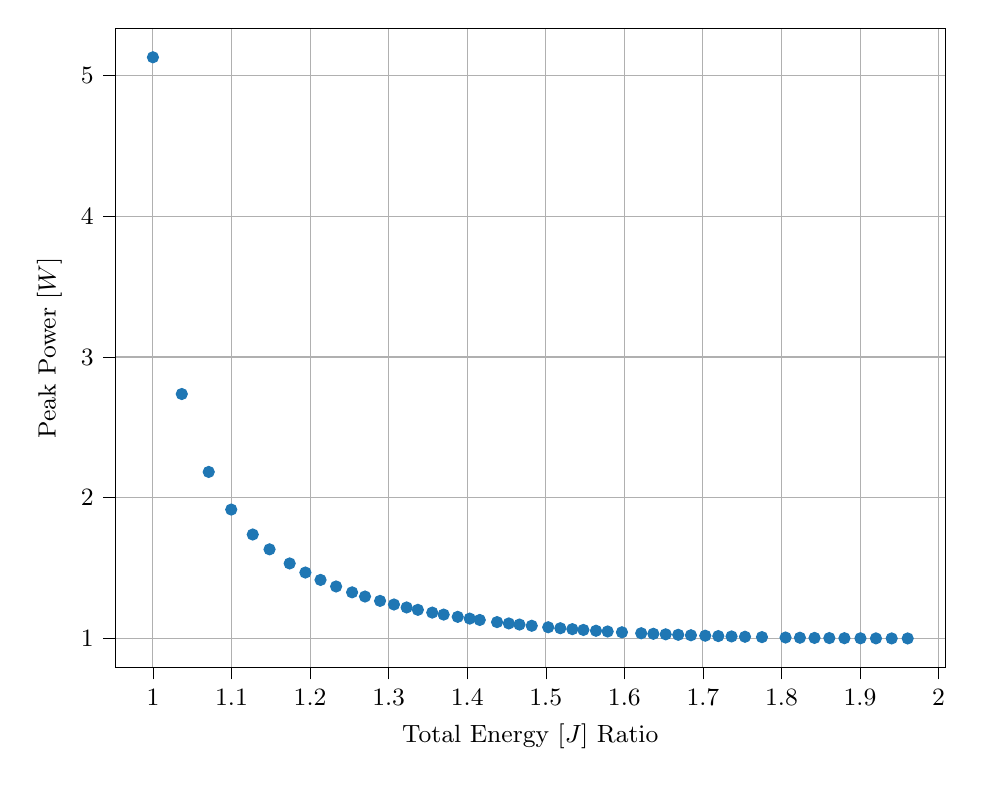
\begin{tikzpicture}

\definecolor{color0}{rgb}{0.12156862745098,0.466666666666667,0.705882352941177}

\begin{axis}[
tick align=outside,
tick pos=left,
%title={Minimum Total Energy-Peak Power Pareto Front},
x grid style={white!69.0196078431373!black},
xlabel={Total Energy [$J$] Ratio},
xmajorgrids,
xmin=0.951969544385374, xmax=2.00863956790714,
xtick style={color=black},
y grid style={white!69.0196078431373!black},
ylabel={Peak Power [$W$]},
ymajorgrids,
ymin=0.793506983229606, ymax=5.33635335217828,
ytick style={color=black},
width=\columnwidth,
height=0.8*\columnwidth,
scatter/classes={a={mark=o,draw=blude,fill=blue}}
]
\addplot [draw=color0, fill=color0, mark=*, only marks, scatter]
table{%
x  y
1.96060911229251 1
1.94025735739117 1.0001722044611
1.92022941641552 1.0005209338863
1.90051914797258 1.00104840496291
1.88010319966055 1.00179943373981
1.86091983474008 1.00270705753225
1.84204341192555 1.00380314173853
1.82346217004409 1.00509101615154
1.80516808270552 1.00657419535713
1.77516465085549 1.00952319054964
1.75356571069214 1.01202998468797
1.73644395014839 1.01429940861698
1.71958098197054 1.01678138261286
1.70297082005988 1.01948129270869
1.6847560029071 1.02275126915254
1.66856844904918 1.02594922527939
1.65262776498959 1.02938413528153
1.63692401135337 1.03306306078131
1.62144838436521 1.03699519261659
1.59695173300746 1.04391393451492
1.57874869726961 1.04959554278909
1.56391713794426 1.05463789934253
1.54787852047451 1.06052045258158
1.53382274519599 1.06607340032231
1.51853154152655 1.07256979509741
1.50309219668518 1.07965044840479
1.48212701741409 1.09013686156188
1.46651934681065 1.09866941642491
1.4529516924511 1.10665694012016
1.43798552897677 1.11611869909273
1.41596721112654 1.1313799157411
1.40322301939178 1.14103305686666
1.38791279277902 1.15351995344745
1.37003803674729 1.16955872989789
1.35549882376095 1.18376353726084
1.33721798248121 1.20333421203095
1.32291260433993 1.22019533614076
1.3067782828274 1.24128269858374
1.28907827174466 1.26687287758902
1.26991954833709 1.29787652349395
1.25350241925129 1.32761325443868
1.2331526541595 1.36927317067809
1.21332027018405 1.41592781493746
1.19403407664326 1.46844271819122
1.1740449855315 1.53296716763917
1.14841534276446 1.63321207078177
1.1270421185732 1.73863123835234
1.09966977869654 1.91587822063535
1.07100508087054 2.1833255626401
1.03673105988299 2.73696111101528
1 5.12986033540788
};
\end{axis}

\end{tikzpicture}
 \caption{Minimum total energy-peak power Pareto front -- normalized to axes
minima}
\label{fig:pareto}
\end{figure}


\section{MULTI-AXIS TRAJECTORY OPTIMIZATION EXAMPLE}

The trajectory optimization framework can be generalized to multi-axis
problems by extension of the problem formulation \eqref{eq:baseProgram}
with new kinematic variables and associated kinematic constraints
\eqref{eq:kinematicConstraints} for each moving body. Also necessary
is the reformulation of the cost and objective function variables
to include coupled effects of the system (e.g., staged motion and
accompanying dynamics).

Here we demonstrate such an extension through and example of a two-link
Selective Compliance Articulated Robotic Arm (SCARA). A SCARA consists
of a fixed rotary joint rotating a link at the end of which another
rotary joint/link pair is situated. In this example, it is clear that
the kinematics of the endpoint of link 2, as well as the joint torque
and power requirements, are coupled and dependent on the relative
motion of the two joints. Derivation of these relationships is straightforward
using Lagrange's equations and will not be reproduced here.

To exercise this example, we define a trajectory generation problem
for the SCARA starting at rest such that the tip velocity $\left\langle v_{x}^{tip},v_{y}^{tip}\right\rangle $
of the second link is equal to $\left\langle 0,v_{f}^{tip}\right\rangle $
at $t_{f}$ (as if it were throwing a baseball). We choose to formulate
the tip velocities as constraints while the cost function minimizes
the equally weighted peak power ($\mathcal{L}_{\infty}$ norm) of
the two joint actuators. In this case we only care about hitting the
velocity target at the end of motion, so the final position and acceleration
constraints $d_{N}$ and $a_{N}$ are removed from the problem formulation.
Note that this does not dictate the position or pose of the SCARA
at the end of motion, only the tip velocity, so there may be many
ways in which the end condition may manifest. An alternative formulation
to this problem could instead add new constraint equations to enforce
the tip velocity at an intermediate point in time.

The solution of this trajectory generation problem is shown through
the following figures. Fig. \ref{fig:SCARA_states} shows the initial
and final positions of the SCARA as well as traces of the tip positons,
Fig. \ref{fig:SCARA_trajectories} shows the motion profiles of the
two joint actuators, and Fig. \ref{fig:SCARA_tip_position-trajectories}
shows the trajectories the link tips. From the motion profiles it
is clear that the position (limited to $\pm\pi$ radians) and jerk
side constraints are being enforced at various points through the
motion, while the peak power cost function manifests as a flattening
of the actuator power curves. An interesting outcome of this example
is that the optimizer plans ``wind-up'' motion for the arm (much
like a pitcher throwing a baseball), which it turns out is required
in order to reach the tip velocities within the given joint position
constraints (i.e., it is not possible to reach the tip speeds if only
forward motion is allowed). The optimization code used for this example,
along with specific link dimensions and properties, is provided on
GitHub at \url{TBDsite}. Readers are encouraged to explore this example
to better understand the relationship between the problem formulation,
variables, and constraints.

\begin{figure}
\centering{}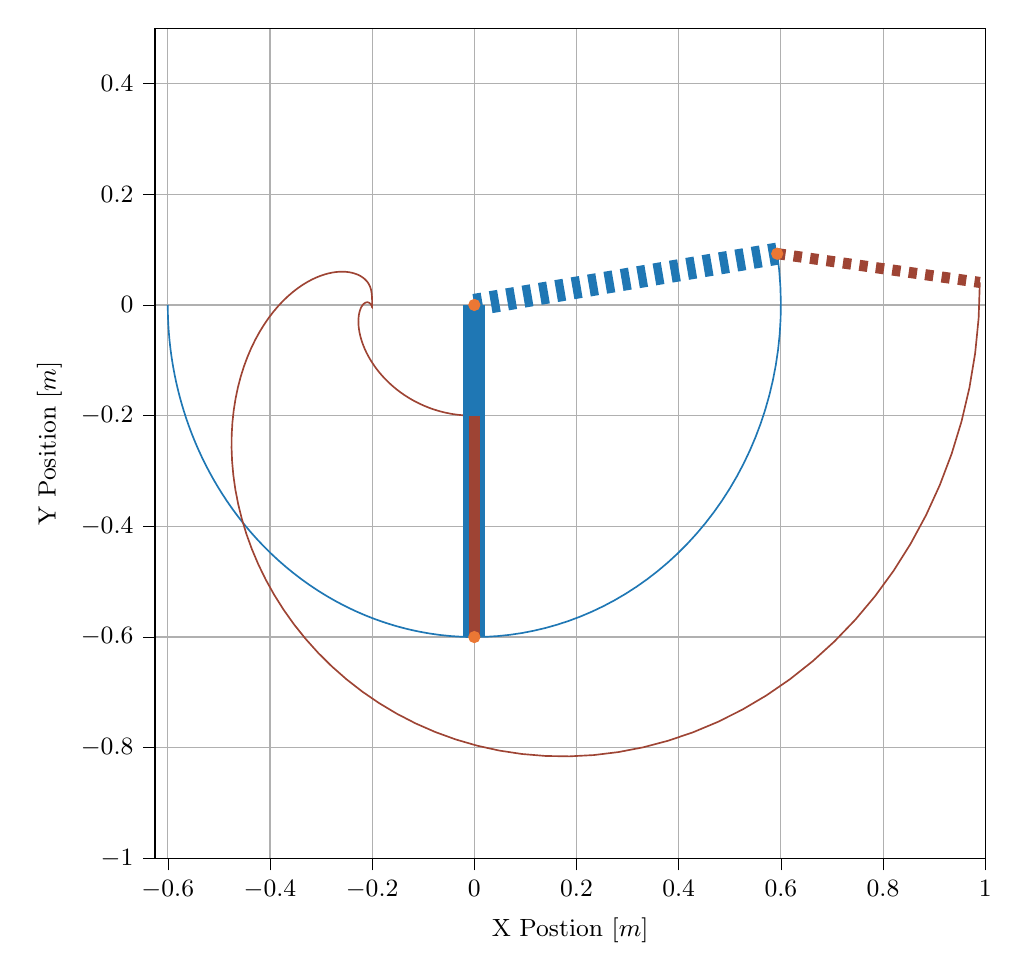
\begin{tikzpicture}

\definecolor{color0}{rgb}{0.12156862745098,0.466666666666667,0.705882352941177}
\definecolor{color1}{rgb}{0.62156862745098,0.266666666666667,0.205882352941177}
\definecolor{color2}{rgb}{0.92156862745098,0.466666666666667,0.205882352941177}
\definecolor{color3}{rgb}{0.12156862745098,0.466666666666667,0.705882352941177}
\definecolor{color4}{rgb}{0.62156862745098,0.266666666666667,0.205882352941177}

\begin{axis}[
width=\columnwidth,
height=\columnwidth,
tick align=outside,
tick pos=left,
x grid style={white!69.0196078431373!black},
xlabel={X Postion [$m$]},
xmajorgrids,
xmin=-0.625, xmax=1.0,
xtick style={color=black},
y grid style={white!69.0196078431373!black},
ylabel={Y Position [$m$]},
ymajorgrids,
ymin=-1.0, ymax=0.5,
ytick style={color=black},
scatter/classes={a={mark=*,draw=black,fill=color2}}
]

\addplot [semithick, color0]
table {%
0.000477796026439958 -0.599999809759101
0.000477796026439958 -0.599999809759101
0.000477796026439958 -0.599999809759101
0.00041006853654841 -0.599999859869813
0.000207634109141991 -0.599999964073396
-0.00019560350227917 -0.599999968116057
-0.000864684292381848 -0.599999376933905
-0.00186336559251155 -0.599997106550247
-0.00325381863989863 -0.599991177155347
-0.00509621133293122 -0.599978356801352
-0.00744811874149606 -0.599953769491627
-0.0103636663988564 -0.599910488672079
-0.0138922497464608 -0.599839149603443
-0.0180765788143499 -0.599727635930152
-0.02294972369488 -0.599560931167407
-0.0285311842391278 -0.599321259030508
-0.0348238336290432 -0.598988564674967
-0.0418150311550916 -0.598541145761508
-0.0494808641595295 -0.597956222546455
-0.0577901410653986 -0.597210431586423
-0.0667071956265104 -0.596280261329894
-0.0761937710563357 -0.595142427702995
-0.0862102996700035 -0.593774186228071
-0.096716772038635 -0.59215358312386
-0.107673311007187 -0.590259653116109
-0.119040528238622 -0.588072574293913
-0.130779722898645 -0.585573790464151
-0.142852970958714 -0.582746109972661
-0.155223144131062 -0.579573787818314
-0.167853888373859 -0.57604259578418
-0.180709583517588 -0.572139883616673
-0.193755298459357 -0.567854633087488
-0.206956750887514 -0.563177505997961
-0.220280276620865 -0.558100886696873
-0.23369281112228 -0.552618919355614
-0.247161884230735 -0.546727539989996
-0.260655628315419 -0.540424502985842
-0.274142799618887 -0.533709401657043
-0.287592812325162 -0.526583682142643
-0.300975784731617 -0.519050649749316
-0.314262596741366 -0.511115466689645
-0.327424957686403 -0.502785140078798
-0.340435483230617 -0.494068499054065
-0.353267779796807 -0.484976159988751
-0.365896534638646 -0.47552047899058
-0.378297609371749 -0.46571549119996
-0.390448134525593 -0.455576836818428
-0.402326602514741 -0.445121674274513
-0.41391295638046 -0.434368581437916
-0.425188671736623 -0.423337446284694
-0.436136829567852 -0.412049348858243
-0.446742177862637 -0.400526436728648
-0.456991180501784 -0.388791796394402
-0.466872052341789 -0.376869323164098
-0.476374780011312 -0.364783591968134
-0.485491128551254 -0.352559731248522
-0.494214634641188 -0.340223301533679
-0.502540587719016 -0.327800179522566
-0.510466000753328 -0.315316447517257
-0.517989572695497 -0.302798286948154
-0.525111644651273 -0.290271873683337
-0.531834151523411 -0.27776327200221
-0.538160570286004 -0.265298323759203
-0.544095865220312 -0.252902529544803
-0.549646429503025 -0.240600919646156
-0.554820021679067 -0.228417914236252
-0.559625694973294 -0.216377174225143
-0.564073717251678 -0.204501446219517
-0.568175479778803 -0.192812406701766
-0.571943393652956 -0.181330511654106
-0.575390773758196 -0.170074858441641
-0.578531711062928 -0.159063067035061
-0.581380934980298 -0.148311187849852
-0.583953668236613 -0.137833643763065
-0.586265477286621 -0.127643214241458
-0.5883321218046 -0.117751069858823
-0.590169407175497 -0.10816686569427
-0.591793044165136 -0.098898902308173
-0.593218519974288 -0.089954363760274
-0.594460984610377 -0.0813396445533221
-0.595535156012221 -0.0730607825957231
-0.596455246931125 -0.065124023281203
-0.597234916674393 -0.0575365475583234
-0.597887251933353 -0.0503073948399588
-0.598424783202909 -0.0434485770601431
-0.598859545362858 -0.0369762752016924
-0.599203186851238 -0.0309118240697771
-0.599467110893425 -0.0252820678958445
-0.599662597488906 -0.0201188760336566
-0.599800841338953 -0.0154580312162988
-0.599892868442443 -0.0113378301230114
-0.599949329506059 -0.00779756533993152
-0.599980187637188 -0.0048759043104134
-0.599994327392647 -0.00260904132680093
-0.599999118859071 -0.001028284171802
-0.599999979708295 -0.000156045010102346
-0.6 -7.34788079488412e-17
-0.599999749491242 -0.000548279533622229
-0.599997386492833 -0.00177093245779821
-0.599989008176914 -0.00363181316734528
-0.599967905124127 -0.00620586987990541
-0.599923706853826 -0.0095679650273493
-0.599841444827761 -0.0137927903973277
-0.599700523740698 -0.0189547309433017
-0.599479866238742 -0.0249777896215725
-0.599157477148874 -0.0317854931784384
-0.598711486655913 -0.0393008364575904
-0.598121101388857 -0.0474462651151831
-0.597366277360901 -0.0561563057187641
-0.596427210715572 -0.0653802899813259
-0.595284348084627 -0.075076926718271
-0.593918390780774 -0.0852111793861326
-0.592310300558431 -0.0957523255716584
-0.590441309135237 -0.106672679101389
-0.58829293188889 -0.117946709532629
-0.585846985567363 -0.129550412973616
-0.583085609685625 -0.14146084892133
-0.579991291260135 -0.153655790852154
-0.576546892556764 -0.166113457260811
-0.572735681562956 -0.17881230121168
-0.568541364928225 -0.191730843542584
-0.563948123144589 -0.204847539408447
-0.558940647759747 -0.218140670856938
-0.553504180431288 -0.231588260162487
-0.54762455364091 -0.245168000052197
-0.541288232894355 -0.25885719794919
-0.534482360236468 -0.272632732070186
-0.527194798911938 -0.28647101773164
-0.51941417900156 -0.300347982600408
-0.511129943861629 -0.314239049909473
-0.502332397190666 -0.328119128873461
-0.493012750543462 -0.341962611701294
-0.483163171107514 -0.355743376727285
-0.472776829551624 -0.369434797277022
-0.461847947750843 -0.383009755957122
-0.450371846186225 -0.396440664113573
-0.438344990812155 -0.40969948624558
-0.425765039178406 -0.422757769193436
-0.412630885588741 -0.435586675942058
-0.39894270507277 -0.448157023898121
-0.38470199594319 -0.460439327509419
-0.369911620706321 -0.472403845101225
-0.354575845090329 -0.484020629806705
-0.338700374952537 -0.495259584467591
-0.322292390825089 -0.506090520377776
-0.30536057985676 -0.516483219736656
-0.287915164908207 -0.526407501671357
-0.26996793055831 -0.535833291677611
-0.251532245780638 -0.544730694318347
-0.232623083051481 -0.553070069007195
-0.213257033654429 -0.560822108691262
-0.193452318951108 -0.567957921233993
-0.173228797393602 -0.57444911328469
-0.152607967061127 -0.580267876406638
-0.131612963511956 -0.585387075220832
-0.110268552751212 -0.589780337307165
-0.0886011191261832 -0.593422144589826
-0.0666386479731188 -0.596287925918607
-0.0444107028531716 -0.598354150543044
-0.0219483972301776 -0.599598422161889
0.000715639540647482 -0.599999573216555
0.0235473020263004 -0.599537759083848
0.0465110544260477 -0.598194551810845
0.0695699822518262 -0.595953033023141
0.0926858500313193 -0.59279788562711
0.115819165063314 -0.588715483917348
0.138929247231095 -0.583693981692292
0.161974304854712 -0.57772339797418
0.184911516537087 -0.570795699924198
0.207697118932134 -0.562904882539929
0.230286500335536 -0.554047044720221
0.25263429997057 -0.544220461282356
0.274694512812593 -0.533425650518094
0.296420599766608 -0.521665436878853
0.317765602982803 -0.508945008385951
0.338682266065368 -0.495271968369731
0.359123158900224 -0.480656381151363
0.379040806797935 -0.465110811293363
0.398387823618933 -0.448650356059337
0.417117048519664 -0.431292670740234
0.435181685930449 -0.413057986523359
0.452535448348849 -0.393969120601737
0.469132701506534 -0.374051478244882
0.484928611443043 -0.353333046577761
0.499879292996708 -0.331844379842587
0.513941959201593 -0.309618575947937
0.527075071059665 -0.286691244141583
0.539238487139901 -0.263100463677035
0.550393612440701 -0.23888673337897
0.560514543912218 -0.214064116710106
0.5695764111642 -0.188633803559465
0.577548410441114 -0.162597151257157
0.584393575040822 -0.135956424824304
0.590063032718495 -0.108745654713429
0.594504905382456 -0.0810180071107489
0.597669556018687 -0.0528308793077023
0.599509915600908 -0.0242458469885549
0.599981814639023 0.00467141332633128
0.599044317544076 0.0338512277200049
0.596660057847661 0.0632200551188162
0.592795572179525 0.0927006451129062
};
\addplot [semithick, color1]
table {%
-0.000477795218472657 -0.200000951204014
-0.000477795218472657 -0.200000951204014
-0.000477795218472657 -0.200000951204014
-0.000541403986433626 -0.200000991496366
-0.000728670160688234 -0.200001059907004
-0.0010946262120739 -0.200000978419624
-0.00168732837194933 -0.200000222863902
-0.00254570854158072 -0.199997688540546
-0.00369849541816139 -0.199991424327219
-0.00516540076188399 -0.199978362785323
-0.00695954562278916 -0.199954067871354
-0.00908955033312515 -0.199912517891913
-0.0115608459812914 -0.199845943965543
-0.0143762663158506 -0.199744751687071
-0.0175359714482617 -0.199597568737031
-0.0210367853126378 -0.199391472712046
-0.0248715627276789 -0.199112393462045
-0.0290296490115531 -0.198745530473592
-0.0334980706344668 -0.198275662209659
-0.0382623766289466 -0.197687382919497
-0.043306928679478 -0.196965313567094
-0.0486148742397135 -0.196094304727359
-0.0541680362044324 -0.195059635011285
-0.0599468564378339 -0.193847201921261
-0.0659304390552466 -0.192443699889992
-0.0720966804923586 -0.190836781396576
-0.0784224505307817 -0.189015199546999
-0.0848837900834984 -0.186968932676324
-0.0914561029115525 -0.184689292738918
-0.0981143298795708 -0.182169019644549
-0.10483310231253 -0.179402363636803
-0.111586875464983 -0.176385157569131
-0.118350045159151 -0.17311488064151
-0.125097051349501 -0.169590714851989
-0.131802472430765 -0.165813595088576
-0.138441113906313 -0.161786253427923
-0.144988094751229 -0.157513257813834
-0.151418934505042 -0.153001044864709
-0.157709643825268 -0.148257946115568
-0.163836820915084 -0.143294206553291
-0.169777755888981 -0.138121993872947
-0.175510544741202 -0.132755396491185
-0.181014214117606 -0.127210408023763
-0.186268857552147 -0.121504895692491
-0.191255783212067 -0.115658549993971
-0.195957672508474 -0.109692812955024
-0.200358748189651 -0.103630782425962
-0.204444949770953 -0.0974970901217418
-0.208204113400863 -0.0913177515015997
-0.211626152548606 -0.0851199860641016
-0.214703235244871 -0.0789320072123822
-0.217429953013694 -0.0727827815119105
-0.219803476077665 -0.0667017579423922
-0.221823688858652 -0.0607185686904826
-0.223493299192005 -0.0548627042263844
-0.224817914020633 -0.049163166953089
-0.225806073724563 -0.0436481096738975
-0.226469236904571 -0.0383444674360916
-0.226821707774023 -0.033277593704045
-0.226880499817523 -0.0284709137457588
-0.226665132447769 -0.0239456088246794
-0.226197362051006 -0.0197203435561844
-0.2255008544727 -0.0158110453108948
-0.224600811521901 -0.0122307392114753
-0.223523568157922 -0.0089894361051136
-0.222296178707285 -0.00609406518879158
-0.22094600945932 -0.00354843880589661
-0.219500351681119 -0.00135323495646347
-0.217986064261173 0.000494016521624174
-0.216429249758551 0.00199895540187103
-0.214854962490523 0.00317042661270375
-0.213286943216942 0.00402052981370821
-0.211747372621017 0.00456467544317057
-0.210256635615841 0.00482163237640992
-0.208833090714939 0.00481354688006511
-0.207492843011879 0.00456591068206563
-0.206249524820591 0.00410745876415319
-0.20511409334466 0.00346998452945931
-0.204094658464938 0.00268806930391335
-0.203196354996848 0.00179873174419411
-0.202421272541899 0.0008410077945087
-0.201768453104871 -0.000144528214283887
-0.201233963258244 -0.00111629504646744
-0.20081104522962 -0.00203228666012457
-0.200490351127546 -0.00285069818872601
-0.200260267633699 -0.0035305610697885
-0.200107345057517 -0.0040322953729819
-0.200016851597515 -0.00431804279497177
-0.199973473257647 -0.00435169584033187
-0.199962167934116 -0.00409866284213442
-0.199969167112868 -0.00352546077349781
-0.199983109835353 -0.00259918844664379
-0.199996288175648 -0.00128700872257545
-0.20000598321999 0.000444567360645285
-0.200014991129221 0.00253507999577519
-0.200032277719453 0.00492700188766781
-0.200071592441246 0.00756761703041431
-0.200149896274425 0.0104105015341072
-0.200285751820929 0.0134148868455636
-0.200498038182391 0.0165415577169321
-0.200808555582433 0.0197134988132443
-0.201240630488141 0.022863572395251
-0.201818722716633 0.0259301586780875
-0.202567969898359 0.0288546267041503
-0.20350889457707 0.0316524991054945
-0.204660872811021 0.0343388530633444
-0.206042225910189 0.0369281059816609
-0.207670287211928 0.0394338920472729
-0.209561868302229 0.0418627756616206
-0.211733370310918 0.0442128172595875
-0.214200562358669 0.0464761409385018
-0.216978388999283 0.0486403617218038
-0.220080789671 0.0506894417780427
-0.223520522555436 0.0526042381705765
-0.227308989213006 0.0543628756046313
-0.231456058294306 0.0559410171964677
-0.235969887678393 0.0573120756317849
-0.240856745020331 0.0584473905165428
-0.246120827104022 0.0593163882996653
-0.251764078689346 0.0598867355453751
-0.257786011764772 0.0601244928715119
-0.26418352629466 0.0599942746530783
-0.270950733699718 0.0594594181194483
-0.278078784437894 0.0584821644620894
-0.28555570116658 0.0570238538465938
-0.29336621906798 0.0550451356838594
-0.301491635009407 0.0525061950950609
-0.309909667289692 0.0493669961618194
-0.318594327791766 0.0455875422594655
-0.327515808419656 0.0411281535096061
-0.336640383744754 0.0359497611463255
-0.345930331820794 0.0300142183603235
-0.355343875148361 0.0232846269617649
-0.364835143777115 0.0157256789821042
-0.374354162526206 0.00730401211552084
-0.383846864279472 -0.00201142231942553
-0.393255131270909 -0.0122489804381891
-0.402516866216594 -0.023433937630708
-0.41156609507058 -0.0355880931681281
-0.420333103083427 -0.0487293697817016
-0.428744605721971 -0.0628714106400192
-0.436723955866898 -0.0780231763680954
-0.444191388539872 -0.0941885449647266
-0.451064304223862 -0.111365917681189
-0.457257591628251 -0.129547834122735
-0.46268399051415 -0.148720600022354
-0.467254494934731 -0.168863931311551
-0.470878796960488 -0.189950618272991
-0.473465770650265 -0.211946213702224
-0.474923995696171 -0.234808749127524
-0.475162319814827 -0.258488483235475
-0.474090458579744 -0.282927686722322
-0.471619630991285 -0.308060467834325
-0.467663228663209 -0.333812642871532
-0.462137516070246 -0.360101655905373
-0.454962358851585 -0.3868365518984
-0.446061976703531 -0.413918007311413
-0.435365716923635 -0.441238422136231
-0.422808844192017 -0.468682077098885
-0.408333341697082 -0.496125359535391
-0.391888718236746 -0.523437061148309
-0.37343281545724 -0.550478750504846
-0.352932608934785 -0.5771052227348
-0.330364996366305 -0.603165028427652
-0.305717565719879 -0.628501083211886
-0.278989335810095 -0.652951358925721
-0.250191461414446 -0.676349656657141
-0.219347894741394 -0.698526461243236
-0.186495994805846 -0.719309876076002
-0.151687076071027 -0.738526636266312
-0.114986887584485 -0.756003197372798
-0.0764760137779825 -0.771566896012107
-0.0362501881236845 -0.785047177736353
0.00557948905008587 -0.796276886598598
0.0488864370741001 -0.80509360983502
0.0935285939667874 -0.811341070081021
0.1393485357417 -0.814870556517294
0.186173723228664 -0.815542385320995
0.233816882993618 -0.813227378788005
0.282076528169496 -0.807808351507391
0.330737624112102 -0.799181591021822
0.379572402769372 -0.78725831951237
0.428341328499475 -0.771966122217932
0.476794216794559 -0.753250327554344
0.524671505965806 -0.731075323252657
0.571705680327155 -0.70542579230677
0.617622841786785 -0.676307852124802
0.662144425026879 -0.643750080033235
0.704989049634976 -0.607804408204549
0.745872804535964 -0.568524714264389
0.784509188370044 -0.525982141753953
0.820611929174799 -0.480276432704342
0.853898167817772 -0.43153598174956
0.884095685161213 -0.379937098711022
0.91094604674972 -0.32569126688832
0.934205541518811 -0.269033401178889
0.953647305295577 -0.21022087009716
0.969063385566799 -0.149532328526726
0.980266731505675 -0.0872663642858299
0.987093093443344 -0.02373996279482
0.989402816236824 0.0407132046943376
};


%\draw[line width=4mm] (0,0)--(0,-1);
%\draw[line width=4mm] (0,-1)--(0,-0.2);
%\draw[fill=gray!30!white] (0,0) circle (4pt);
%\draw[fill=gray!50!white] (0,-1) circle (4pt);


\addplot [line width=8pt, color0]
table {%
0.0 0.0
0.0 -0.6
};

\addplot [line width=4pt, color1]
table {%
0.0 -0.6
0.0 -0.2
};


\addplot [line width=8pt, color3,dashed]
table {%
0.0 0.0
0.592795572179525 0.0927006451129062
};

\addplot [line width=4pt, color4,dashed]
table {%
0.592795572179525 0.0927006451129062
0.989402816236824 0.0407132046943376
};

%\addplot+[draw=black,fill=color2,mark=*,only marks,mark size=8pt,scatter] coordinates {(0,0)};

%\addplot[draw=black,mark color=color2,mark=*,only marks,mark size=8pt,scatter]
%\addplot[draw=color0,mark=*,only marks,mark size=8pt,scatter]
\addplot [draw=color2, fill=color2, mark=*, only marks, scatter]
table{%
0 0
0 -.6
0.5928 0.0926
};

%\draw[fill=gray!50!white] (0.5,0) circle (4pt);


\end{axis}

\end{tikzpicture}
\caption{SCARA in-plane motion with starting (solid) and ending (dashed) poses}
\label{fig:SCARA_states}
\end{figure}
\begin{figure}
\centering{}% This file was created by tikzplotlib v0.9.8.
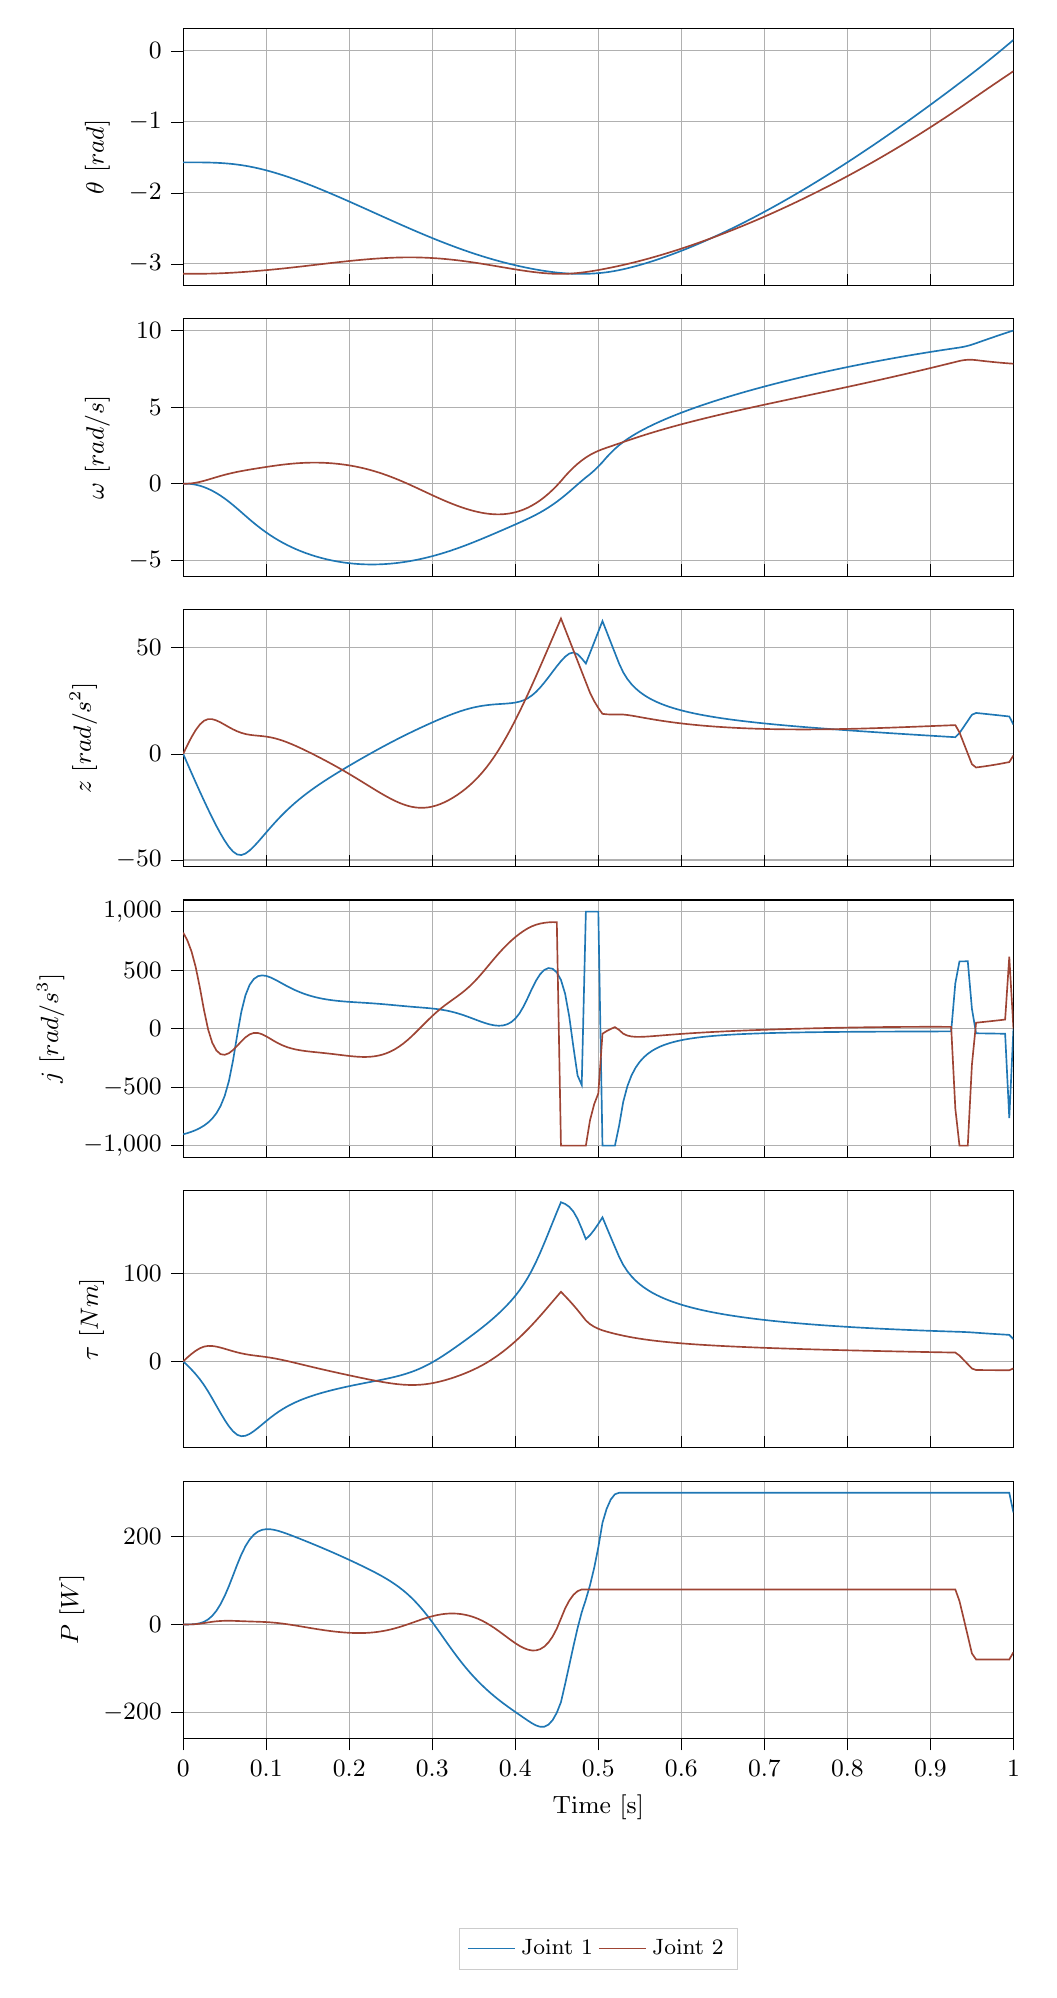
\begin{tikzpicture}

\definecolor{color0}{rgb}{0.12156862745098,0.466666666666667,0.705882352941177}
\definecolor{color1}{rgb}{0.62156862745098,0.266666666666667,0.205882352941177}

\begin{groupplot}[group style={group size=1 by 6,vertical sep=12}]
\nextgroupplot[
ytick align=outside,
xticklabels={},
tick pos=left,
%title={Minimum Mixed Objective - Joint 1},
x grid style={white!69.0196078431373!black},
xmajorgrids,
xmin=0, xmax=1,
xtick style={color=black},
y grid style={white!69.0196078431373!black},
ylabel={$\theta$ [$rad$]},
ymajorgrids,
ymin=-3.30642840851841, ymax=0.31995819991115,
ytick style={color=black}
]
\addplot [semithick, color0]
table {%
0 -1.57
0.005 -1.57
0.01 -1.57
0.015 -1.57011287918078
0.02 -1.57045026993942
0.025 -1.5711223326378
0.03 -1.57223746778105
0.035 -1.57390194110794
0.04 -1.57621938444297
0.045 -1.57929011447932
0.05 -1.58321017686492
0.055 -1.58806996312716
0.06 -1.59395214564412
0.065 -1.60092851769356
0.07 -1.60905519911862
0.075 -1.61836623946249
0.08 -1.62886868453084
0.085 -1.64054458374416
0.09 -1.65335819841688
0.095 -1.66726277482438
0.1 -1.68220531052612
0.105 -1.69812975957811
0.11 -1.71497920304232
0.115 -1.73269730996162
0.12 -1.75122928348873
0.125 -1.77052242402704
0.13 -1.79052641082816
0.135 -1.81119338452522
0.14 -1.83247789696777
0.145 -1.85433677936606
0.15 -1.87672896563498
0.155 -1.89961529590668
0.16 -1.92295831599308
0.165 -1.94672208208886
0.17 -1.97087197579456
0.175 -1.99537453204033
0.18 -2.02019728115991
0.185 -2.04530860575528
0.19 -2.0706776127782
0.195 -2.0962740212102
0.2 -2.1220680657052
0.205 -2.14803041648208
0.21 -2.17413211557597
0.215 -2.20034452926592
0.22 -2.22663931610343
0.225 -2.2529884095043
0.23 -2.27936401337583
0.235 -2.30573860878283
0.24 -2.33208496925481
0.245 -2.35837618204068
0.25 -2.38458567245349
0.255 -2.41068722843179
0.26 -2.43665502259028
0.265 -2.46246362935853
0.27 -2.48808803534227
0.275 -2.51350364182208
0.28 -2.53868625935456
0.285 -2.56361209575132
0.29 -2.58825774020805
0.295 -2.6126001478859
0.3 -2.63661663057565
0.305 -2.66028485990827
0.31 -2.68358288961734
0.315 -2.70648920238714
0.32 -2.72898278478852
0.325 -2.75104323091205
0.33 -2.77265087200629
0.335 -2.79378692630465
0.34 -2.81443366079448
0.345 -2.83457455517192
0.35 -2.85419445749282
0.355 -2.87327972066804
0.36 -2.89181830852977
0.365 -2.90979985948048
0.37 -2.9272156947735
0.375 -2.94405875750692
0.38 -2.96032346763844
0.385 -2.97600547756887
0.39 -2.99110131115904
0.395 -3.00560786465204
0.4 -3.01952173901137
0.405 -3.03283835969479
0.41 -3.04555082691889
0.415 -3.05764844294694
0.42 -3.06911492063564
0.425 -3.07992645246432
0.43 -3.09005012825174
0.435 -3.09944339475724
0.44 -3.10805490678689
0.445 -3.11582641729447
0.45 -3.122695145305
0.455 -3.12859634550488
0.46 -3.1334660569572
0.465 -3.13724423767464
0.47 -3.13987884579784
0.475 -3.14133257857002
0.48 -3.14159265358979
0.485 -3.14067885423991
0.49 -3.13864109520795
0.495 -3.13553959468075
0.5 -3.13124935269654
0.505 -3.12564536927821
0.51 -3.11860264445587
0.515 -3.10999617829033
0.52 -3.09995097061095
0.525 -3.0885920213894
0.53 -3.07604433061215
0.535 -3.06243289827115
0.54 -3.04786162525438
0.545 -3.03240870010086
0.55 -3.01613559662927
0.555 -2.99909223300056
0.56 -2.98132016457493
0.565 -2.96285467589272
0.57 -2.94372621372607
0.575 -2.92396140457621
0.58 -2.90358379880891
0.585 -2.88261442858083
0.59 -2.86107223513804
0.595 -2.83897440214129
0.6 -2.81633661989609
0.605 -2.79317329779911
0.61 -2.76949773731356
0.615 -2.74532227440267
0.62 -2.72065839800891
0.625 -2.69551684951567
0.63 -2.66990770694302
0.635 -2.64384045676503
0.64 -2.61732405559711
0.645 -2.59036698352293
0.65 -2.56297729046752
0.655 -2.53516263674416
0.66 -2.50693032868753
0.665 -2.47828735011641
0.67 -2.44924039023619
0.675 -2.4197958684858
0.68 -2.38995995674845
0.685 -2.35973859927715
0.69 -2.32913753063038
0.695 -2.29816229186762
0.7 -2.2668182452168
0.705 -2.23511058739497
0.71 -2.20304436173749
0.715 -2.17062446926941
0.72 -2.1378556788346
0.725 -2.10474263638309
0.73 -2.07128987350352
0.735 -2.03750181527723
0.74 -2.00338278752053
0.745 -1.96893702347379
0.75 -1.93416866998904
0.755 -1.89908179326153
0.76 -1.86368038414571
0.765 -1.82796836309126
0.77 -1.79194958473105
0.775 -1.75562784214918
0.78 -1.71900687085447
0.785 -1.68209035248171
0.79 -1.64488191824091
0.795 -1.60738515213247
0.8 -1.56960359394435
0.805 -1.53154074204574
0.81 -1.49320005598994
0.815 -1.45458495893825
0.82 -1.41569883991497
0.825 -1.37654505590293
0.83 -1.33712693378766
0.835 -1.29744777215767
0.84 -1.25751084296728
0.845 -1.21731939306783
0.85 -1.17687664561244
0.855 -1.13618580133869
0.86 -1.09525003973324
0.865 -1.0540725200818
0.87 -1.01265638240731
0.875 -0.971004748298821
0.88 -0.929120721633248
0.885 -0.887007389191577
0.89 -0.844667821170948
0.895 -0.802105071593653
0.9 -0.759322178613782
0.905 -0.716322164722011
0.91 -0.673108036848773
0.915 -0.629682786365809
0.92 -0.586049388985935
0.925 -0.542210804560601
0.93 -0.498169976774681
0.935 -0.453929832737599
0.94 -0.409493282469291
0.945 -0.364811844729095
0.95 -0.319813657862681
0.955 -0.274426822690785
0.96 -0.228579336236811
0.965 -0.182249991008384
0.97 -0.135443751659166
0.975 -0.0881656423698616
0.98 -0.0404207509022215
0.985 0.00778576753681837
0.99 0.0564486866167315
0.995 0.105562705389566
1 0.155122444982534
};
\addplot [semithick, color1]
table {%
0 -3.14
0.005 -3.14
0.01 -3.14
0.015 -3.13989741765331
0.02 -3.13959794763312
0.025 -3.13901908908014
0.03 -3.13809490095493
0.035 -3.13678118107675
0.04 -3.13505790376708
0.045 -3.13292589233212
0.05 -3.13040023662025
0.055 -3.12750431280825
0.06 -3.12426537715456
0.065 -3.12071137588474
0.07 -3.1168685751201
0.075 -3.11275983458486
0.08 -3.10840354087863
0.085 -3.10381329714698
0.09 -3.09899840571724
0.095 -3.09396502964681
0.1 -3.08871775679897
0.105 -3.08326120604013
0.11 -3.07760135623038
0.115 -3.07174641751002
0.12 -3.06570722670896
0.125 -3.05949726379295
0.13 -3.05313242791481
0.135 -3.04663069803092
0.14 -3.04001176665763
0.145 -3.03329669920066
0.15 -3.0265076444761
0.155 -3.01966760509174
0.16 -3.0128002667792
0.165 -3.00592988088332
0.17 -2.99908119203849
0.175 -2.99227940232721
0.18 -2.98555016318565
0.185 -2.97891958658719
0.19 -2.97241426739087
0.195 -2.96606130909507
0.2 -2.95988834556473
0.205 -2.95392355162119
0.21 -2.94819563573906
0.215 -2.94273380853805
0.22 -2.93756772133893
0.225 -2.93272736981144
0.23 -2.9282429586887
0.235 -2.92414472464418
0.24 -2.92046271568098
0.245 -2.91722652672072
0.25 -2.91446499246627
0.255 -2.91220584006703
0.26 -2.91047530573062
0.265 -2.90929772138728
0.27 -2.90869508006505
0.275 -2.90868659199192
0.28 -2.90928824761959
0.285 -2.91051240834981
0.29 -2.91236744968675
0.295 -2.91485748314769
0.3 -2.91798218061584
0.305 -2.92173671661543
0.31 -2.92611183052757
0.315 -2.93109399433441
0.32 -2.9366656556988
0.325 -2.94280551459373
0.33 -2.94948878649957
0.335 -2.95668740692152
0.34 -2.96437013993051
0.345 -2.97250256629806
0.35 -2.98104694311251
0.355 -2.98996194497546
0.36 -2.99920231510044
0.365 -3.00871847031704
0.37 -3.01845611384197
0.375 -3.02835591048755
0.38 -3.03835326922025
0.385 -3.04837825932092
0.39 -3.058355663556
0.395 -3.06820515077781
0.4 -3.07784153653832
0.405 -3.08717509660805
0.41 -3.09611190440786
0.415 -3.10455417624622
0.42 -3.1124006242105
0.425 -3.11954683214271
0.43 -3.12588567939038
0.435 -3.13130782650914
0.44 -3.1357022349957
0.445 -3.13895665048321
0.45 -3.14095799658648
0.455 -3.14159265358979
0.46 -3.14074689086929
0.465 -3.13830697363477
0.47 -3.13439793313035
0.475 -3.12914476932845
0.48 -3.12267248221591
0.485 -3.11510607178531
0.49 -3.10657053803213
0.495 -3.09719088095252
0.5 -3.08709210053616
0.505 -3.07637199812982
0.51 -3.06511133390899
0.515 -3.05337930753974
0.52 -3.04118134744322
0.525 -3.02852008048955
0.53 -3.01539582158616
0.535 -3.00180693469679
0.54 -2.98775478607834
0.545 -2.97324476970565
0.55 -2.95828429384427
0.555 -2.94288172447777
0.56 -2.92704580177562
0.565 -2.91078530814736
0.57 -2.89410887717649
0.575 -2.87702488442009
0.58 -2.85954138704782
0.585 -2.84166609312749
0.59 -2.823406349069
0.595 -2.80476913818979
0.6 -2.78576108601442
0.605 -2.76638846953852
0.61 -2.74665722869426
0.615 -2.72657297889294
0.62 -2.7061410239301
0.625 -2.68536636880433
0.63 -2.66425373217498
0.635 -2.64280755829807
0.64 -2.62103202835475
0.645 -2.59893107113555
0.65 -2.57650837307574
0.655 -2.55376738765714
0.66 -2.53071134420427
0.665 -2.50734325611
0.67 -2.48366592852967
0.675 -2.45968196558396
0.68 -2.43539377711103
0.685 -2.41080358500715
0.69 -2.38591342919357
0.695 -2.3607251732454
0.7 -2.33524050971627
0.705 -2.30946096518995
0.71 -2.28338790508858
0.715 -2.25702253826433
0.72 -2.23036592139991
0.725 -2.20341896324106
0.73 -2.1761824286824
0.735 -2.14865694272645
0.74 -2.12084299433407
0.745 -2.09274094018274
0.75 -2.06435100834835
0.755 -2.03567330192431
0.76 -2.00670780259085
0.765 -1.97745437414645
0.77 -1.94791276601187
0.775 -1.91808261671665
0.78 -1.88796345737701
0.785 -1.85755471517288
0.79 -1.82685571683156
0.795 -1.79586569212412
0.8 -1.76458377738055
0.805 -1.73300901902852
0.81 -1.70114037716022
0.815 -1.6689767291311
0.82 -1.63651687319369
0.825 -1.60375953216928
0.83 -1.57070335715949
0.835 -1.53734693129958
0.84 -1.50368877355456
0.845 -1.46972734255897
0.85 -1.43546104050059
0.855 -1.40088821704815
0.86 -1.36600717332246
0.865 -1.33081616591028
0.87 -1.29531341091973
0.875 -1.2594970880759
0.88 -1.22336534485475
0.885 -1.18691630065345
0.89 -1.15014805099478
0.895 -1.11305867176308
0.9 -1.07564622346909
0.905 -1.0379087555406
0.91 -0.999844310635966
0.915 -0.96145092897706
0.92 -0.922726652698382
0.925 -0.883669530208739
0.93 -0.844277620562001
0.935 -0.804548997833546
0.94 -0.764481755499833
0.945 -0.724161197135832
0.95 -0.683712322704384
0.955 -0.643260132177822
0.96 -0.602929625518666
0.965 -0.562759258997298
0.97 -0.52274269247031
0.975 -0.482873134486347
0.98 -0.443143330192024
0.985 -0.403545550387642
0.99 -0.364071581843231
0.995 -0.324712718985456
1 -0.285459757065662
};
\nextgroupplot[
ytick align=outside,
xticklabels={},
tick pos=left,
x grid style={white!69.0196078431373!black},
xmajorgrids,
xmin=0, xmax=1,
xtick style={color=black},
y grid style={white!69.0196078431373!black},
ylabel={$\omega$ [$rad/s$]},
ymajorgrids,
ymin=-6.03887681302138, ymax=10.7637560387153,
ytick style={color=black}
]
\addplot [semithick, color0]
table {%
0 0
0.005 0
0.01 -0.0225758361552111
0.015 -0.0674781517286859
0.02 -0.134412539676749
0.025 -0.223027028648849
0.03 -0.332894665378337
0.035 -0.463488667006789
0.04 -0.614146007270252
0.045 -0.784012477118403
0.05 -0.971957252448655
0.055 -1.17643650339168
0.06 -1.39527440988757
0.065 -1.62533628501276
0.07 -1.86220806877498
0.075 -2.10048901366958
0.08 -2.33517984266386
0.085 -2.56272293454296
0.09 -2.78091528150075
0.095 -2.98850714034799
0.1 -3.1848898103973
0.105 -3.36988869284268
0.11 -3.54362138385971
0.115 -3.70639470542186
0.12 -3.85862810766187
0.125 -4.00079736022403
0.13 -4.1333947394128
0.135 -4.256902488509
0.14 -4.37177647965888
0.145 -4.47843725378349
0.15 -4.5772660543407
0.155 -4.66860401727917
0.16 -4.75275321915627
0.165 -4.82997874114024
0.17 -4.9005112491543
0.175 -4.96454982391478
0.18 -5.02226491907566
0.185 -5.07380140458404
0.19 -5.11928168639838
0.195 -5.15880889900085
0.2 -5.19247015537512
0.205 -5.22033981877969
0.21 -5.24248273798893
0.215 -5.2589573675014
0.22 -5.26981868017512
0.225 -5.27512077430608
0.23 -5.27491908140035
0.235 -5.26927209439546
0.24 -5.25824255717386
0.245 -5.24189808256129
0.25 -5.22031119566009
0.255 -5.19355883169884
0.26 -5.16172135365046
0.265 -5.12488119674818
0.27 -5.08312129596093
0.275 -5.03652350649515
0.28 -4.98516727935264
0.285 -4.92912889134549
0.29 -4.86848153557124
0.295 -4.80329653795017
0.3 -4.73364586652394
0.305 -4.65960594181301
0.31 -4.58126255396115
0.315 -4.49871648027486
0.32 -4.4120892247073
0.325 -4.32152821884773
0.33 -4.22721085967067
0.335 -4.12934689796618
0.34 -4.02817887548851
0.345 -3.92398046418071
0.35 -3.81705263504283
0.355 -3.70771757234731
0.36 -3.59631019014031
0.365 -3.4831670586043
0.37 -3.36861254668541
0.375 -3.25294202630328
0.38 -3.13640198608535
0.385 -3.01916671803549
0.39 -2.90131069859891
0.395 -2.78277487186667
0.4 -2.66332413668319
0.405 -2.54249344482035
0.41 -2.41952320561024
0.415 -2.29329553774032
0.42 -2.16230636573614
0.425 -2.0247351574834
0.43 -1.87865330109897
0.435 -1.72230240593019
0.44 -1.55430210151673
0.445 -1.37374560210557
0.45 -1.18024003997542
0.455 -0.973942290464104
0.46 -0.75563614348896
0.465 -0.526921624640262
0.47 -0.290746554436484
0.475 -0.0520212712500388
0.48 0.182766137271944
0.485 0.407551806392695
0.49 0.620300105439345
0.495 0.858048396843142
0.5 1.1207966836663
0.505 1.40854496446759
0.51 1.72129323310795
0.515 2.00904153587541
0.52 2.27178984431108
0.525 2.50953815544996
0.53 2.72228646819866
0.535 2.91425460335451
0.54 3.09058503070482
0.545 3.25462069431738
0.55 3.4086727257418
0.555 3.55441368512555
0.56 3.69309773644274
0.565 3.82569243333025
0.57 3.95296182997108
0.575 4.07552115346134
0.58 4.19387404561577
0.585 4.30843868855742
0.59 4.41956659935033
0.595 4.52755644903916
0.6 4.63266441939752
0.605 4.73511209710987
0.61 4.83509258217703
0.615 4.93277527875247
0.62 5.02830969864861
0.625 5.1218285145293
0.63 5.21345003559694
0.635 5.30328023358549
0.64 5.39141441483495
0.645 5.47793861108291
0.65 5.56293074467224
0.655 5.64646161132454
0.66 5.72859571422512
0.665 5.80939197604461
0.67 5.88890435007671
0.675 5.96718234746991
0.68 6.04427149426104
0.685 6.12021372935306
0.69 6.19504775255207
0.695 6.26880933016491
0.7 6.34153156436541
0.705 6.413245131495
0.71 6.4839784936178
0.715 6.55375808696059
0.72 6.62260849030265
0.725 6.69055257591437
0.73 6.75761164525765
0.735 6.82380555134012
0.74 6.88915280934714
0.745 6.95367069695025
0.75 7.01737534550173
0.755 7.08028182316437
0.76 7.14240421088983
0.765 7.20375567204336
0.77 7.26434851637357
0.775 7.32419425894171
0.78 7.38330367455172
0.785 7.44168684815991
0.79 7.49935322168883
0.795 7.55631163762295
0.8 7.61257037972292
0.805 7.6681372111596
0.81 7.7230194103382
0.815 7.77722380465527
0.82 7.83075680240797
0.825 7.88362442305343
0.83 7.93583232599796
0.835 7.98738583807917
0.84 8.0382899798897
0.845 8.08854949107808
0.85 8.13816885475083
0.855 8.1871523210895
0.86 8.23550393028693
0.865 8.2832275348987
0.87 8.33032682169791
0.875 8.37680533311454
0.88 8.42266648833433
0.885 8.46791360412578
0.89 8.51254991545897
0.895 8.5565785959742
0.9 8.60000277835405
0.905 8.64282557464773
0.91 8.68505009659271
0.915 8.72667947597492
0.92 8.76771688506681
0.925 8.80816555718405
0.93 8.84802880741625
0.935 8.88731005366158
0.94 8.93628754803926
0.945 8.99963737328286
0.95 9.07736703437906
0.955 9.1694972907948
0.96 9.26586904568557
0.965 9.36124786984343
0.97 9.45562185786097
0.975 9.54897829352802
0.98 9.64130368780797
0.985 9.73258381598263
0.99 9.8228037545669
0.995 9.91194791859357
1 10
};
\addplot [semithick, color1]
table {%
0 0
0.005 0
0.01 0.020516469338524
0.015 0.0598940040370316
0.02 0.115771710597382
0.025 0.184837625040748
0.03 0.262743975636348
0.035 0.344655461934501
0.04 0.426402286991318
0.045 0.505131142374277
0.05 0.579184762400392
0.055 0.647787130738449
0.06 0.710800253962521
0.065 0.768560152928662
0.07 0.821748107048686
0.075 0.871258741245196
0.08 0.918048746330147
0.085 0.962978285947511
0.09 1.00667521408665
0.095 1.04945456956732
0.1 1.09131015176819
0.105 1.13196996195102
0.11 1.17098774407128
0.115 1.20783816021155
0.12 1.24199258320206
0.125 1.27296717562742
0.13 1.30034597677918
0.135 1.32378627465696
0.14 1.34301349139485
0.145 1.35781094491267
0.15 1.36800787687084
0.155 1.37346766250761
0.16 1.3740771791762
0.165 1.36973776896741
0.17 1.36035794225564
0.175 1.34584782831103
0.18 1.32611531969203
0.185 1.30106383926473
0.19 1.27059165916043
0.195 1.23459270606672
0.2 1.19295878870921
0.205 1.14558317642448
0.21 1.09236544020245
0.215 1.03321743982364
0.22 0.96807030549927
0.225 0.896882224547802
0.23 0.819646808903922
0.235 0.736401792638801
0.24 0.647237792053754
0.245 0.552306850888738
0.25 0.451830479848233
0.255 0.346106867281535
0.26 0.235516868669003
0.265 0.120528264445232
0.27 0.00169761462601879
0.275 -0.120331125533092
0.28 -0.244832146044246
0.285 -0.371008267388481
0.29 -0.498006692188279
0.295 -0.624939493629992
0.3 -0.750907199916919
0.305 -0.875022782429543
0.31 -0.996432761367298
0.315 -1.11433227287815
0.32 -1.22797177898493
0.325 -1.33665438116861
0.33 -1.43972408438908
0.335 -1.53654660179958
0.34 -1.62648527351018
0.345 -1.70887536288924
0.35 -1.78300037259089
0.355 -1.84807402499578
0.36 -1.90323104331853
0.365 -1.94752870498672
0.37 -1.9799593291157
0.375 -1.99947174654065
0.38 -2.00499802013432
0.385 -1.99548084701513
0.39 -1.96989744436257
0.395 -1.92727715210255
0.4 -1.86671201394579
0.405 -1.78736155996225
0.41 -1.68845436767206
0.415 -1.56928959285413
0.42 -1.42924158644235
0.425 -1.26776944953382
0.43 -1.08442942375311
0.435 -0.878881697311297
0.44 -0.650883097503069
0.445 -0.400269220652453
0.45 -0.126937666544502
0.455 0.169158809981411
0.46 0.487983446905052
0.465 0.781808100883143
0.47 1.0506327603793
0.475 1.29445742250949
0.48 1.5132820861201
0.485 1.70710675063432
0.49 1.8759314159232
0.495 2.0197560832715
0.5 2.14402048126865
0.505 2.25213284416484
0.51 2.34640527385028
0.515 2.43959201930419
0.52 2.53225339073417
0.525 2.62485178067759
0.53 2.71777737787381
0.535 2.81042972369117
0.54 2.90200327453808
0.545 2.99209517227518
0.55 3.08051387330068
0.555 3.16718454042891
0.56 3.25209872565191
0.565 3.33528619417508
0.57 3.4167985512805
0.575 3.49669947445312
0.58 3.57505878406637
0.585 3.65194881169697
0.59 3.72744217584316
0.595 3.80161043507382
0.6 3.8745232951795
0.605 3.94624816885283
0.61 4.01684996026382
0.615 4.08639099256725
0.62 4.15493102515378
0.625 4.22252732587064
0.63 4.28923477538108
0.635 4.3551059886643
0.64 4.42019144384073
0.645 4.48453961196236
0.65 4.54819708372012
0.655 4.61120869057398
0.66 4.67361761885251
0.665 4.73546551606641
0.67 4.79679258914219
0.675 4.85763769458538
0.68 4.91803842077591
0.685 4.97803116271759
0.69 5.0376511896327
0.695 5.096932705827
0.7 5.15590890526281
0.705 5.21461202027483
0.71 5.27307336485101
0.715 5.33132337288302
0.72 5.38939163176957
0.725 5.44730691173314
0.73 5.50509719118839
0.735 5.56278967847738
0.74 5.62041083026624
0.745 5.67798636687683
0.75 5.735541284809
0.755 5.79309986669094
0.76 5.85068568887954
0.765 5.90832162691788
0.77 5.96602985904343
0.775 6.02383186792863
0.78 6.08174844082408
0.785 6.1397996682645
0.79 6.19800494148849
0.795 6.25638294871426
0.8 6.31495167040621
0.805 6.37372837365958
0.81 6.43272960582405
0.815 6.49197118748086
0.82 6.55146820488243
0.825 6.61123500195776
0.83 6.67128517198205
0.835 6.73163154900398
0.84 6.7922861991194
0.845 6.85326041167584
0.85 6.91456469048764
0.855 6.97620874513761
0.86 7.03820148243665
0.865 7.10055099810893
0.87 7.16326456876611
0.875 7.2263486442301
0.88 7.28980884025997
0.885 7.35364993173463
0.89 7.41787584633914
0.895 7.4824896587983
0.9 7.54749358569767
0.905 7.6128889809275
0.91 7.67867633178133
0.915 7.74485525573547
0.92 7.81142449792859
0.925 7.87838192934767
0.93 7.94572454569101
0.935 8.01344846674253
0.94 8.06411167280031
0.945 8.08977488628949
0.95 8.09043810531255
0.955 8.06610133183115
0.96 8.03407330427352
0.965 8.00331330539772
0.97 7.97391159679249
0.975 7.94596085886458
0.98 7.9195559608764
0.985 7.89479370888234
0.99 7.8717725715549
0.995 7.85059238395886
1 7.83135402952509
};
\nextgroupplot[
ytick align=outside,
xticklabels={},
tick pos=left,
x grid style={white!69.0196078431373!black},
xmajorgrids,
xmin=0, xmax=1,
xtick style={color=black},
y grid style={white!69.0196078431373!black},
ylabel={$z$ [$rad/s^2$]},
ymajorgrids,
ymin=-53.1664811142691, ymax=68.0599458634201,
ytick style={color=black}
]
\addplot [semithick, color0]
table {%
0 0
0.005 -4.51516723104222
0.01 -8.98046311469496
0.015 -13.3868775896127
0.02 -17.7228977944199
0.025 -21.9735273458976
0.03 -26.1188003256904
0.035 -30.1314680526927
0.04 -33.97329396963
0.045 -37.5889550660505
0.05 -40.8958501886047
0.055 -43.7675812991783
0.06 -46.0123750250381
0.065 -47.3743567524444
0.07 -47.6561889789196
0.075 -46.9381657988563
0.08 -45.5086183758198
0.085 -43.6384693915585
0.09 -41.5183717694474
0.095 -39.2765340098624
0.1 -36.9997764890759
0.105 -34.7465382034061
0.11 -32.5546643124298
0.115 -30.4466804480024
0.12 -28.4338505124311
0.125 -26.5194758377534
0.13 -24.701549819242
0.135 -22.9747982299741
0.14 -21.3321548249232
0.145 -19.7657601114416
0.15 -18.2675925876937
0.155 -16.8298403754209
0.16 -15.4451043967931
0.165 -14.1065016028119
0.17 -12.8077149520955
0.175 -11.5430190321763
0.18 -10.3072971016774
0.185 -9.09605636286774
0.19 -7.9054425204932
0.195 -6.73225127485516
0.2 -5.57393268091344
0.205 -4.42858384184819
0.21 -3.29492590249269
0.215 -2.17226253474375
0.22 -1.06041882619282
0.225 0.0403385811455988
0.23 1.12939740097807
0.235 2.20590744432104
0.24 3.26889492251312
0.245 4.31737738024056
0.25 5.3504727922497
0.255 6.36749560967544
0.26 7.36803138045613
0.265 8.35198015744934
0.27 9.31955789315611
0.275 10.2712454285019
0.28 11.2076776014302
0.285 12.1294711548512
0.29 13.0369995242139
0.295 13.9301342852452
0.3 14.8079849421867
0.305 15.6686775703723
0.31 16.5092147372566
0.315 17.3254511135117
0.32 18.1122011719144
0.325 18.8634718354125
0.33 19.5727923408985
0.335 20.2336044955335
0.34 20.8396822615607
0.345 21.3855658275748
0.35 21.8670125391038
0.355 22.2814764414016
0.36 22.6286263072015
0.365 22.9109023837769
0.37 23.1341040764276
0.375 23.308008043586
0.38 23.447053609971
0.385 23.5712038873167
0.39 23.7071653464483
0.395 23.8901470366942
0.4 24.1661383725685
0.405 24.5940478420223
0.41 25.2455335739846
0.415 26.197834400835
0.42 27.5142416505486
0.425 29.216371276886
0.43 31.2701790337562
0.435 33.6000608826911
0.44 36.1112998822327
0.445 38.701112426029
0.45 41.259549902264
0.455 43.6612293950288
0.46 45.7429037697396
0.465 47.2350140407557
0.47 47.745056637289
0.475 46.9574817043965
0.48 44.9571338241503
0.485 42.5496598093299
0.49 47.5496582807596
0.495 52.5496573646321
0.5 57.5496561602579
0.505 62.5496537280706
0.51 57.5496605534932
0.515 52.5496616871338
0.52 47.5496622277764
0.525 42.5496625497403
0.53 38.3936270311702
0.535 35.2660854700602
0.54 32.807132722512
0.545 30.8104062848851
0.55 29.1481918767502
0.555 27.7368102634384
0.56 26.5189393775016
0.565 25.453879328166
0.57 24.5118646980516
0.575 23.6705784308853
0.58 22.9129285883297
0.585 22.2255821585819
0.59 21.5979699377679
0.595 21.0215940716711
0.6 20.4895355424693
0.605 19.9960970134327
0.61 19.5365393150889
0.615 19.1068839792276
0.62 18.7037631761377
0.625 18.3243042135274
0.63 17.9660395977113
0.635 17.6268362498912
0.64 17.3048392495909
0.645 16.9984267178677
0.65 16.7061733304599
0.655 16.426820580116
0.66 16.1592523638983
0.665 15.902474806419
0.67 15.65559947864
0.675 15.4178293582271
0.68 15.188447018403
0.685 14.9668046398017
0.69 14.7523155225685
0.695 14.5444468401005
0.7 14.3427134259184
0.705 14.1466724245596
0.71 13.9559186685576
0.715 13.7700806684122
0.72 13.588817122344
0.725 13.4118138686548
0.73 13.2387812164954
0.735 13.0694516014037
0.74 12.9035775206218
0.745 12.7409297102962
0.75 12.5812955325274
0.755 12.4244775450929
0.76 12.2702922307047
0.765 12.1185688660422
0.77 11.9691485136288
0.775 11.8218831220023
0.78 11.6766347216374
0.785 11.5332747057839
0.79 11.3916831868249
0.795 11.2517484199934
0.8 11.1133662873368
0.805 10.9764398357182
0.81 10.8408788634147
0.815 10.7065995505408
0.82 10.5735241290924
0.825 10.4415805889047
0.83 10.3107024162419
0.835 10.1808283621067
0.84 10.0519022376762
0.845 9.92387273455013
0.85 9.7966932677334
0.855 9.67032183948651
0.86 9.54472092235442
0.865 9.41985735984071
0.87 9.29570228332756
0.875 9.17223104395736
0.88 9.04942315829027
0.885 8.92726226663779
0.89 8.80573610304605
0.895 8.68483647596889
0.9 8.5645592587358
0.905 8.44490438899607
0.91 8.32587587644192
0.915 8.20748181837802
0.92 8.08973442344794
0.925 7.97265004643998
0.93 7.85624924906713
0.935 9.79549887553562
0.94 12.669965048721
0.945 15.5459322192384
0.95 18.4260512831481
0.955 19.2743509781556
0.96 19.0757648315717
0.965 18.8747976035074
0.97 18.6712871334094
0.975 18.4650788559903
0.98 18.2560256349311
0.985 18.0439877168543
0.99 17.8288328053349
0.995 17.6104362417684
1 13.7878019894015
};
\addplot [semithick, color1]
table {%
0 0
0.005 4.10329386770479
0.01 7.87550693970152
0.015 11.1755413120701
0.02 13.8131828886733
0.025 15.5812701191199
0.03 16.3822972596306
0.035 16.3493650113633
0.04 15.7457710765919
0.045 14.8107240052229
0.05 13.7204736676113
0.055 12.6026246448145
0.06 11.5519797932282
0.065 10.6375908240047
0.07 9.90212683930213
0.075 9.35800101699009
0.08 8.9859079234729
0.085 8.73938562782842
0.09 8.55587109613329
0.095 8.37111644017468
0.1 8.13196203656536
0.105 7.80355642405163
0.11 7.37008322805382
0.115 6.83088459810272
0.12 6.19491848507264
0.125 5.47576023035074
0.13 4.68805957555649
0.135 3.84544334757785
0.14 2.959490703565
0.145 2.03938639163307
0.15 1.09195712735432
0.155 0.121903333718381
0.16 -0.867882041758136
0.165 -1.87596534235355
0.17 -2.90202278892271
0.175 -3.94650172380071
0.18 -5.01029608545944
0.185 -6.09443602085994
0.19 -7.19979061874249
0.195 -8.32678347150202
0.2 -9.47512245694661
0.205 -10.6435472444051
0.21 -11.829600075762
0.215 -13.0294268648739
0.22 -14.2376161902936
0.225 -15.4470831287761
0.23 -16.6490032530241
0.235 -17.8328001170094
0.24 -18.9861882330032
0.245 -20.0952742081011
0.25 -21.1447225133395
0.255 -22.1179997225063
0.26 -22.9977208447542
0.265 -23.7661299638427
0.27 -24.4057480318223
0.275 -24.9002041022308
0.28 -25.2352242688469
0.285 -25.3996849599597
0.29 -25.3865602883425
0.295 -25.1935412573854
0.3 -24.8231165025248
0.305 -24.281995787551
0.31 -23.5799023021699
0.315 -22.727901221357
0.32 -21.7365204367346
0.325 -20.6139406440956
0.33 -19.3645034820993
0.335 -17.9877343421197
0.34 -16.4780178758122
0.345 -14.8250019403295
0.35 -13.0147304809795
0.355 -11.0314036645487
0.36 -8.85953233363813
0.365 -6.48612482579643
0.37 -3.90248348498941
0.375 -1.1052547187354
0.38 1.90343462383808
0.385 5.11668053051323
0.39 8.52405845200373
0.395 12.1130276313517
0.4 15.8700907967074
0.405 19.7814384580385
0.41 23.8329549635861
0.415 28.0096012823556
0.42 32.2944273817066
0.425 36.6680051561417
0.43 41.109545288363
0.435 45.5997199616455
0.44 50.1227753701234
0.445 54.66631082159
0.45 59.2192953051827
0.455 63.7649273847281
0.46 58.7649307956183
0.465 53.7649318992315
0.47 48.764932426038
0.475 43.7649327221219
0.48 38.7649329028446
0.485 33.7649330577753
0.49 28.7649334696602
0.495 24.8528795994299
0.5 21.6224725792373
0.505 18.8544859370896
0.51 18.6373490907812
0.515 18.5322742859956
0.52 18.5196779886851
0.525 18.5851194392438
0.53 18.5304691634708
0.535 18.3147101693816
0.54 18.018379547421
0.545 17.6837402050997
0.55 17.3341334256456
0.555 16.9828370445999
0.56 16.6374937046349
0.565 16.3024714210839
0.57 15.980184634523
0.575 15.6718619226504
0.58 15.3780055261205
0.585 15.0986728292371
0.59 14.8336518461331
0.595 14.5825720211357
0.6 14.344974734667
0.605 14.1203582821967
0.61 13.9082064606858
0.615 13.7080065173063
0.62 13.5192601433716
0.625 13.3414899020892
0.63 13.1742426566425
0.635 13.0170910352877
0.64 12.8696336243241
0.645 12.7314943515533
0.65 12.6023213707714
0.655 12.4817856557072
0.66 12.3695794427793
0.665 12.2654146151554
0.67 12.1690210886393
0.675 12.0801452381053
0.68 11.9985483883363
0.685 11.9240053830219
0.69 11.8563032388597
0.695 11.7952398871628
0.7 11.7406230024031
0.705 11.6922689152351
0.71 11.6500016064038
0.715 11.6136517773087
0.72 11.5830559927152
0.725 11.5580558910482
0.73 11.5384974577994
0.735 11.5242303577707
0.74 11.5151073221181
0.745 11.510983586434
0.75 11.5117163763879
0.755 11.5171644377216
0.76 11.5271876076674
0.765 11.5416464251092
0.77 11.5604017770401
0.775 11.5833145790895
0.78 11.6102454880857
0.785 11.6410546447971
0.79 11.6756014451539
0.795 11.7137443383905
0.8 11.7553406506745
0.805 11.8002464328927
0.81 11.8483163313624
0.815 11.8994034803144
0.82 11.9533594150659
0.825 12.0100340048579
0.83 12.0692754043851
0.835 12.1309300230848
0.84 12.1948425112877
0.845 12.2608557623606
0.85 12.328810929994
0.855 12.3985474598074
0.86 12.4699031344559
0.865 12.5427141314362
0.87 12.6168150927985
0.875 12.6920392059734
0.88 12.7682182949327
0.885 12.8451829209008
0.89 12.9227624918336
0.895 13.0007853798732
0.9 13.0790790459654
0.905 13.157470170767
0.91 13.2357847908272
0.915 13.3138484386242
0.92 13.3914862838165
0.925 13.4685232686674
0.93 13.5447842103036
0.935 10.1326412115557
0.94 5.13264269783651
0.945 0.132643804611892
0.95 -4.8673546962793
0.955 -6.40560551152696
0.96 -6.15199977515932
0.965 -5.8803417210451
0.97 -5.59014758558312
0.975 -5.28097959763668
0.98 -4.95245039881114
0.985 -4.60422746548883
0.99 -4.23603751920801
0.995 -3.84767088675325
1 -0.773250069206286
};
\nextgroupplot[
ytick align=outside,
xticklabels={},
tick pos=left,
x grid style={white!69.0196078431373!black},
xmajorgrids,
xmin=0, xmax=1,
xtick style={color=black},
y grid style={white!69.0196078431373!black},
ylabel={$j$ [$rad/s^3$]},
ymajorgrids,
ymin=-1099.99992322631, ymax=1099.99980439359,
ytick style={color=black}
]
\addplot [semithick, color0]
table {%
0 -903.033446208443
0.005 -893.059176730549
0.01 -881.282894983545
0.015 -867.204040961453
0.02 -850.125910295529
0.025 -829.054595958553
0.03 -802.533545400471
0.035 -768.36518338746
0.04 -723.132219284094
0.045 -661.379024510848
0.05 -574.346222114716
0.055 -448.958745171954
0.06 -272.396345481268
0.065 -56.3664452950326
0.07 143.604636012663
0.075 285.909484607299
0.08 374.029796852256
0.085 424.019524422212
0.09 448.367551917015
0.095 455.351504157292
0.1 450.647657133959
0.105 438.374778195253
0.11 421.596772885493
0.115 402.565987114257
0.12 382.874934935538
0.125 363.585203702284
0.13 345.350317853569
0.135 328.528681010178
0.14 313.278942696327
0.145 299.633504749574
0.15 287.550442454566
0.155 276.947195725564
0.16 267.720558796232
0.165 259.757330143274
0.17 252.939183983848
0.175 247.14438609978
0.18 242.248147761933
0.185 238.122768474907
0.19 234.638249127608
0.195 231.663718788345
0.2 229.069767813049
0.205 226.731587871101
0.21 224.532673549787
0.215 222.368741710187
0.22 220.151481467683
0.225 217.811763966495
0.23 215.302008668594
0.235 212.597495638415
0.24 209.696491545489
0.245 206.619082401828
0.25 203.404563485146
0.255 200.10715415614
0.26 196.789755398642
0.265 193.515547141352
0.27 190.337507069159
0.275 187.286434585669
0.28 184.358710684195
0.285 181.505673872527
0.29 178.626952206278
0.295 175.570131388296
0.3 172.138525637113
0.305 168.107433376863
0.31 163.247275251019
0.315 157.350011680528
0.32 150.254132699629
0.325 141.864101097196
0.33 132.162430927014
0.335 121.215553205424
0.34 109.176713202836
0.345 96.2893423057942
0.35 82.8927804595544
0.355 69.4299731599868
0.36 56.4552153150648
0.365 44.6403385301411
0.37 34.7807934316893
0.375 27.8091132769965
0.38 24.8300554691502
0.385 27.1922918263148
0.39 36.5963380491762
0.395 55.1982671748562
0.4 85.5818938907602
0.405 130.297146392468
0.41 190.460165370081
0.415 263.281449942722
0.42 340.425925267479
0.425 410.761551374043
0.43 465.976369786978
0.435 502.247799908314
0.44 517.962508759262
0.445 511.687495246998
0.45 480.335898552962
0.455 416.33487494215
0.46 298.422054203234
0.465 102.008519306651
0.47 -157.514986578498
0.475 -400.069576049238
0.48 -481.49480296408
0.485 999.999694285935
0.49 999.999816774508
0.495 999.999759125155
0.5 999.999513562536
0.505 -999.998634915478
0.51 -999.999773271874
0.515 -999.999891871484
0.52 -999.999935607219
0.525 -831.207103714017
0.53 -625.508312222001
0.535 -491.790549509643
0.54 -399.34528752538
0.545 -332.442881626972
0.55 -282.276322662367
0.555 -243.574177187366
0.56 -213.012009867107
0.565 -188.402926022874
0.57 -168.257253433267
0.575 -151.529968511114
0.58 -137.469285949563
0.585 -125.522444162806
0.59 -115.275173219359
0.595 -106.411705840368
0.6 -98.68770580732
0.605 -91.9115396687502
0.61 -85.9310671722588
0.615 -80.624160617977
0.62 -75.8917925220736
0.625 -71.6529231632114
0.63 -67.8406695640303
0.635 -64.3994000600418
0.64 -61.2825063446577
0.645 -58.4506774815576
0.65 -55.8705500687771
0.655 -53.5136432435271
0.66 -51.3555114958724
0.665 -49.3750655557988
0.67 -47.5540240825802
0.675 -45.8764679648189
0.68 -44.3284757202614
0.685 -42.897823446628
0.69 -41.5737364936142
0.695 -40.3466828364113
0.7 -39.2082002717664
0.705 -38.1507512004003
0.71 -37.1676000290737
0.715 -36.2527092136452
0.72 -35.4006507378292
0.725 -34.6065304318934
0.73 -33.8659230183405
0.735 -33.1748161563717
0.74 -32.5295620651321
0.745 -31.9268355537508
0.75 -31.3635974868971
0.755 -30.8370628776465
0.76 -30.3446729325019
0.765 -29.8840704826682
0.77 -29.4530783253166
0.775 -29.0496800729802
0.78 -28.67200317069
0.785 -28.3183037918031
0.79 -27.9869533663062
0.795 -27.6764265313102
0.8 -27.3852903237305
0.805 -27.1121944606945
0.81 -26.8558625747797
0.815 -26.6150842896802
0.82 -26.3887080375389
0.825 -26.1756345325528
0.83 -25.9748108270514
0.835 -25.7852248860938
0.84 -25.605900625214
0.845 -25.4358933633462
0.85 -25.2742856493768
0.855 -25.1201834264176
0.86 -24.9727125027437
0.865 -24.8310153026299
0.87 -24.694247874039
0.875 -24.561577133418
0.88 -24.4321783304952
0.885 -24.3052327183489
0.89 -24.1799254154325
0.895 -24.0554434466168
0.9 -23.9309739479459
0.905 -23.8057025108306
0.91 -23.6788116127804
0.915 -23.5494789860153
0.92 -23.416875401593
0.925 -23.2801594745695
0.93 387.849925293699
0.935 574.89323463708
0.94 575.193434103479
0.945 576.023812781933
0.95 169.659939001499
0.955 -39.7172293167687
0.96 -40.1934456128655
0.965 -40.7020940196074
0.97 -41.2416554838074
0.975 -41.8106442118376
0.98 -42.4075836153615
0.985 -43.0309823038905
0.99 -43.6793127133072
0.995 -764.52685047338
1 0
};
\addplot [semithick, color1]
table {%
0 820.658773540958
0.005 754.442614399346
0.01 660.006874473718
0.015 527.528315320634
0.02 353.617446089331
0.025 160.205428102138
0.03 -6.58644965345756
0.035 -120.718786954286
0.04 -187.009414273795
0.045 -218.050067522329
0.05 -223.569804559366
0.055 -210.128970317245
0.06 -182.877793844708
0.065 -147.092796940513
0.07 -108.825164462408
0.075 -74.418618703437
0.08 -49.3044591288973
0.085 -36.7029063390247
0.09 -36.9509311917231
0.095 -47.8308807218631
0.1 -65.6811225027469
0.105 -86.6946391995616
0.11 -107.839725990219
0.115 -127.193222606016
0.12 -143.831650944381
0.125 -157.54013095885
0.13 -168.523245595726
0.135 -177.190528802571
0.14 -184.020862386386
0.145 -189.48585285575
0.15 -194.010758727187
0.155 -197.957075095303
0.16 -201.616660119082
0.165 -205.211489313833
0.17 -208.895786975599
0.175 -212.758872331746
0.18 -216.8279870801
0.185 -221.070919576511
0.19 -225.398570551905
0.195 -229.667797088919
0.2 -233.684957491706
0.205 -237.210566271376
0.21 -239.965357822375
0.215 -241.637865083938
0.22 -241.893387696497
0.225 -240.384024849604
0.23 -236.759372797065
0.235 -230.677623198752
0.24 -221.81719501959
0.245 -209.889661047681
0.25 -194.655441833366
0.255 -175.944224449576
0.26 -153.681823817689
0.265 -127.923613595916
0.27 -98.8912140817068
0.275 -67.004033323214
0.28 -32.8921382225709
0.285 2.62493432344642
0.29 38.6038061914217
0.295 74.0849509721113
0.3 108.224142994755
0.305 140.418697076237
0.31 170.400216162577
0.315 198.276156924467
0.32 224.515958527798
0.325 249.887432399259
0.33 275.353827995921
0.335 301.943293261513
0.34 330.603187096528
0.345 362.054291870011
0.35 396.665363286165
0.355 434.374266182105
0.36 474.681501568341
0.365 516.728268161403
0.37 559.445753250802
0.375 601.737868514697
0.38 642.64918133503
0.385 681.475584298099
0.39 717.793835869594
0.395 751.412633071142
0.4 782.269532266215
0.405 810.303301109524
0.41 835.32926375389
0.415 856.965219870201
0.42 874.715554887037
0.425 888.308026444248
0.43 898.034934656509
0.435 904.611081695574
0.44 908.70709029333
0.445 910.596896718536
0.45 909.126415909076
0.455 -999.999317821966
0.46 -999.999779277352
0.465 -999.999894638712
0.47 -999.999940783207
0.475 -999.999963855458
0.48 -999.999969013862
0.485 -999.999917623026
0.49 -782.410774046057
0.495 -646.081404038521
0.5 -553.59732842955
0.505 -43.4273692616795
0.51 -21.01496095711
0.515 -2.51925946209455
0.52 13.0882901117306
0.525 -10.9300551546071
0.53 -43.1517988178376
0.535 -59.266124392103
0.54 -66.9278684642714
0.545 -69.9213558908209
0.55 -70.2592762091399
0.555 -69.0686679930028
0.56 -67.0044567101939
0.565 -64.4573573121799
0.57 -61.6645423745224
0.575 -58.7712793059718
0.58 -55.8665393766778
0.585 -53.0041966207997
0.59 -50.2159649994879
0.595 -47.5194572937366
0.6 -44.9232904940582
0.605 -42.4303643021809
0.61 -40.0399886759076
0.615 -37.7492747869394
0.62 -35.5540482564722
0.625 -33.4494490893403
0.63 -31.4303242709588
0.635 -29.4914821927219
0.64 -27.6278545541745
0.645 -25.8345961563664
0.65 -24.1071430128398
0.655 -22.4412425855931
0.66 -20.8329655247713
0.665 -19.2787053032131
0.67 -17.7751701068057
0.675 -16.3193699538053
0.68 -14.9086010628849
0.685 -13.5404288324283
0.69 -12.2126703393787
0.695 -10.9233769519489
0.7 -9.67081743359033
0.705 -8.45346176626293
0.71 -7.26996581902248
0.715 -6.11915691869314
0.72 -5.00002033340325
0.725 -3.91168664975579
0.73 -2.85342000573885
0.735 -1.82460713053207
0.74 -0.824747136808028
0.745 0.146557990780015
0.75 1.089612266729
0.755 2.00463398917214
0.76 2.8917634883554
0.765 3.75107038617125
0.77 4.5825604098841
0.775 5.38618179924354
0.78 6.16183134228388
0.785 6.90936007134768
0.79 7.62857864733012
0.795 8.31926245680268
0.8 8.98115644363917
0.805 9.6139796939304
0.81 10.2174297904111
0.815 10.7911869502963
0.82 11.334917958396
0.825 11.8482799054364
0.83 12.3309237399451
0.835 12.7824976405845
0.84 13.2026502145632
0.845 13.5910335266879
0.85 13.9473059626876
0.855 14.2711349296859
0.86 14.5621993960754
0.865 14.8201922724563
0.87 15.0448226349722
0.875 15.2358177918597
0.88 15.3929251936252
0.885 15.5159141865562
0.89 15.6045776079318
0.895 15.6587332184367
0.9 15.6782249603159
0.905 15.6629240120388
0.91 15.6127295593945
0.915 15.5275690384645
0.92 15.4073969701729
0.925 15.2521883272448
0.93 -682.428599749583
0.935 -999.999702743833
0.94 -999.999778644923
0.945 -999.999700178239
0.95 -307.650163049532
0.955 50.7211472735289
0.96 54.3316108228435
0.965 58.0388270923966
0.97 61.833597589287
0.975 65.7058397651075
0.98 69.6445866644633
0.985 73.6379892561639
0.99 77.673326490951
0.995 614.884163509393
1 0
};
\nextgroupplot[
ytick align=outside,
xticklabels={},
tick pos=left,
x grid style={white!69.0196078431373!black},
xmajorgrids,
xmin=0, xmax=1,
xtick style={color=black},
y grid style={white!69.0196078431373!black},
ylabel={$\tau$ [$N\-m$]},
ymajorgrids,
ymin=-98.7262071918525, ymax=194.874694553455,
ytick style={color=black}
]
\addplot [semithick, color0]
table {%
0 0
0.005 -4.5537041292354
0.01 -9.36580657911386
0.015 -14.5710706053145
0.02 -20.3529953424618
0.025 -26.907734285519
0.03 -34.3051007219487
0.035 -42.353541847906
0.04 -50.7006138663444
0.045 -58.9865185572077
0.05 -66.8647565020973
0.055 -73.95252454349
0.06 -79.7689013254123
0.065 -83.7275611884355
0.07 -85.3807116579749
0.075 -84.8628865093029
0.08 -82.7580638288481
0.085 -79.6467458608121
0.09 -75.9689538506134
0.095 -72.0442731687871
0.1 -68.0998133430044
0.105 -64.2878470970223
0.11 -60.6999784534673
0.115 -57.3813660543564
0.12 -54.3444833280555
0.125 -51.5809263745944
0.13 -49.0704678589061
0.135 -46.7873855695034
0.14 -44.7045379988243
0.145 -42.7957697878868
0.15 -41.0371725680784
0.155 -39.4076131579099
0.16 -37.8888248410348
0.165 -36.4652594567697
0.17 -35.1238235197984
0.175 -33.8535688721423
0.18 -32.6453732718618
0.185 -31.491624375064
0.19 -30.3859080064483
0.195 -29.3226956294401
0.2 -28.2970245423772
0.205 -27.3041661215292
0.21 -26.3392812579425
0.215 -25.397066922682
0.22 -24.471402497808
0.225 -23.5550082201921
0.23 -22.6391302813698
0.235 -21.7132679716204
0.24 -20.7649587954587
0.245 -19.779639574707
0.25 -18.7406073520204
0.255 -17.6291148173273
0.26 -16.4246500849123
0.265 -15.1054649295339
0.27 -13.6494187531566
0.275 -12.0351830571467
0.28 -10.2437895254767
0.285 -8.26040189122203
0.29 -6.0760687547117
0.295 -3.68911894738221
0.3 -1.10584909485839
0.305 1.65974634653326
0.31 4.58726481769919
0.315 7.65206126655151
0.32 10.8279869203148
0.325 14.0903165050818
0.33 17.4184703787027
0.335 20.7981869159891
0.34 24.2228916645214
0.345 27.6941293938605
0.35 31.2210639880765
0.355 34.8192077739269
0.36 38.508711422691
0.365 42.3126945942961
0.37 46.2561597758668
0.375 50.3659600321251
0.38 54.6721252794573
0.385 59.2106923810009
0.39 64.0280696168343
0.395 69.1868046870163
0.4 74.7721913191331
0.405 80.8978897594293
0.41 87.7055603304175
0.415 95.3480652071613
0.42 103.944614975945
0.425 113.518172609585
0.43 123.96571058983
0.435 135.093342276121
0.44 146.669135592722
0.445 158.447431036401
0.45 170.16821012163
0.455 181.529199019578
0.46 179.575137626416
0.465 176.303862810597
0.47 170.839498406335
0.475 162.478384999903
0.48 151.41027720134
0.485 139.432599839645
0.49 143.971911295743
0.495 149.9471171251
0.5 156.823483358987
0.505 164.313433527482
0.51 152.878262354283
0.515 141.595000679193
0.52 130.436707458271
0.525 119.383108682368
0.53 110.053246433373
0.535 102.803805712194
0.54 96.9384312212506
0.545 92.0526515664998
0.55 87.8924112494013
0.555 84.2885752183772
0.56 81.1233514073224
0.565 78.311696732057
0.57 75.7903766009685
0.575 73.5112037549291
0.58 71.4366866490925
0.585 69.5371311535674
0.59 67.7886529186179
0.595 66.1717793512368
0.6 64.6704443292005
0.605 63.2712511053695
0.61 61.9629224235826
0.615 60.7358839024284
0.62 59.581943966143
0.625 58.494044835264
0.63 57.4660665732345
0.635 56.492671267045
0.64 55.5691779316228
0.645 54.6914611931447
0.65 53.8558685628627
0.655 53.0591523812264
0.66 52.2984134391993
0.665 51.5710539692657
0.67 50.8747382110555
0.675 50.2073591433622
0.68 49.5670102690725
0.685 48.9519615660737
0.69 48.3606388927469
0.695 47.7916062737303
0.7 47.2435505994379
0.705 46.7152683581944
0.71 46.2056540878748
0.715 45.7136902884961
0.72 45.2384385811996
0.725 44.779031934737
0.73 44.3346678096543
0.735 43.9046020941819
0.74 43.4881437254494
0.745 43.0846499058442
0.75 42.6935218377923
0.755 42.3142009114559
0.76 41.9461652892315
0.765 41.5889268388184
0.77 41.2420283732798
0.775 40.9050411621404
0.78 40.5775626823451
0.785 40.2592145819651
0.79 39.9496408330146
0.795 39.6485060527153
0.8 39.3554939751019
0.805 39.0703060570658
0.81 38.792660204833
0.815 38.5222896085237
0.82 38.2589416738665
0.825 38.0023770413874
0.83 37.7523686844774
0.835 37.5087010786903
0.84 37.2711694354561
0.845 37.0395789941213
0.85 36.8137443668711
0.855 36.5934889316543
0.86 36.3786442687301
0.865 36.1690496368987
0.87 35.9645514858709
0.875 35.7650030015772
0.88 35.5702636815297
0.885 35.3801989376249
0.89 35.1946797240233
0.895 35.0135821879611
0.9 34.8367873415488
0.905 34.6641807527892
0.91 34.4956522542042
0.915 34.3310956676042
0.92 34.1704085436565
0.925 34.0134919150061
0.93 33.8602500617426
0.935 33.7105902879695
0.94 33.5258312107804
0.945 33.2898377528303
0.95 33.0047762594034
0.955 32.6731617336529
0.96 32.3333371671799
0.965 32.0039029164909
0.97 31.6844806729585
0.975 31.3747145295867
0.98 31.0742693843284
0.985 30.7828294806378
0.99 30.500097070188
0.995 30.2257911843876
1 25.4698897119929
};
\addplot [semithick, color1]
table {%
0 0
0.005 4.43069444553649
0.01 8.50370884266897
0.015 12.0652411011788
0.02 14.9068889919546
0.025 16.8005426377143
0.03 17.6353254503515
0.035 17.5485063798044
0.04 16.8174204156109
0.045 15.693277804567
0.05 14.3597724266259
0.055 12.9494581811213
0.06 11.5623597227532
0.065 10.2756468242886
0.07 9.14378025868641
0.075 8.19098532693991
0.08 7.40611022250757
0.085 6.74743539090893
0.09 6.15496725319723
0.095 5.56594967779831
0.1 4.92857271526172
0.105 4.20979488806246
0.11 3.39624887076561
0.115 2.49022110338242
0.12 1.50383310768824
0.125 0.453784152239416
0.13 -0.642371528140243
0.135 -1.76842209356853
0.14 -2.91056535387169
0.145 -4.05776301894793
0.15 -5.20169295072953
0.155 -6.33649719780601
0.16 -7.45844005142135
0.165 -8.56553732241026
0.17 -9.65718694898232
0.175 -10.7338137522732
0.18 -11.7965320444264
0.185 -12.8468254684983
0.19 -13.8862419850557
0.195 -14.9161022351897
0.2 -15.9372209432334
0.205 -16.9496430741714
0.21 -17.9523986514373
0.215 -18.9432819795886
0.22 -19.9186620627104
0.225 -20.8733310095212
0.23 -21.800396267295
0.235 -22.6912212001556
0.24 -23.5354178736356
0.245 -24.3208972796118
0.25 -25.033986885809
0.255 -25.6596338132036
0.26 -26.1817229426172
0.265 -26.5835488894998
0.27 -26.8484816327066
0.275 -26.9608474225529
0.28 -26.9070002457439
0.285 -26.6764842564618
0.29 -26.263101755994
0.295 -25.6656419017708
0.3 -24.8880347316877
0.305 -23.9387913166521
0.31 -22.8297464394664
0.315 -21.574274718422
0.32 -20.1852511048526
0.325 -18.6730557396567
0.33 -17.0438979176695
0.335 -15.2986804249021
0.34 -13.4325612488816
0.345 -11.4352986374184
0.35 -9.29237999253216
0.355 -6.98682223784999
0.36 -4.50138973908427
0.365 -1.82083858992102
0.37 1.06626774803265
0.375 4.16655647624506
0.38 7.48184720251941
0.385 11.0101040627303
0.39 14.7470734239746
0.395 18.6882130161507
0.4 22.8304839817879
0.405 27.1735556221433
0.41 31.7197693266531
0.415 36.471751082119
0.42 41.4266569780463
0.425 46.5688998213928
0.43 51.867985894351
0.435 57.2849376220764
0.44 62.7799692517938
0.445 68.3149228648713
0.45 73.8513744372727
0.455 79.3409731012757
0.46 74.4431334503856
0.465 69.4024526036998
0.47 64.1248796963045
0.475 58.5350938520839
0.48 52.654060169051
0.485 46.6757264216985
0.49 42.475138999658
0.495 39.4505297076802
0.5 37.1640327780006
0.505 35.3799944419042
0.51 33.9585187841163
0.515 32.6613823069192
0.52 31.4662221195349
0.525 30.3561701813112
0.53 29.3182393248601
0.535 28.3516954494217
0.54 27.4570495206343
0.545 26.6303185689849
0.55 25.865959677734
0.555 25.1581322851187
0.56 24.5012388510997
0.565 23.8901380601019
0.57 23.3202064612333
0.575 22.7873308064647
0.58 22.2878706253808
0.585 21.8186102181612
0.59 21.3767092556546
0.595 20.9596561830239
0.6 20.5652261170526
0.605 20.1914436830967
0.61 19.8365506425356
0.615 19.4989779010552
0.62 19.177321398415
0.625 18.8703213754233
0.63 18.5768445482816
0.635 18.2958687705818
0.64 18.0264698169189
0.645 17.7678099734592
0.65 17.5191281672857
0.655 17.2797314071209
0.66 17.0489873431164
0.665 16.8263177832598
0.67 16.6111930291722
0.675 16.4031269152919
0.68 16.2016724532525
0.685 16.0064179981989
0.69 15.816983866317
0.695 15.6330193433606
0.7 15.4542000328009
0.705 15.2802254996551
0.71 15.1108171723223
0.715 14.9457164700525
0.72 14.7846831281603
0.725 14.6274936968992
0.73 14.4739401931539
0.735 14.3238288868667
0.74 14.1769792064731
0.745 14.0332227496459
0.75 13.892402387381
0.755 13.7543714509531
0.76 13.6189929925615
0.765 13.4861391115987
0.77 13.3556903394447
0.775 13.2275350765294
0.78 13.1015690761388
0.785 12.9776949700796
0.79 12.8558218318775
0.795 12.7358647736746
0.8 12.617744573424
0.805 12.5013873293583
0.81 12.386724139046
0.815 12.2736908006455
0.82 12.1622275342291
0.825 12.0522787212837
0.83 11.9437926607018
0.835 11.8367213397592
0.84 11.7310202187451
0.845 11.6266480280502
0.85 11.5235665766557
0.855 11.4217405710791
0.86 11.3211374439376
0.865 11.2217271913851
0.87 11.123482218758
0.875 11.0263771938421
0.88 10.9303889072343
0.885 10.8354961393293
0.89 10.7416795335092
0.895 10.6489214751413
0.9 10.5572059760104
0.905 10.466518563778
0.91 10.3768461759505
0.915 10.2881770574717
0.92 10.2005006599042
0.925 10.1138075359924
0.93 10.0280892041373
0.935 6.64006985846648
0.94 1.73283569575195
0.945 -3.19985797785178
0.95 -8.16263564181518
0.955 -9.87843205078907
0.96 -9.91781316101061
0.965 -9.95593164373436
0.97 -9.99264170989967
0.975 -10.0277919825009
0.98 -10.0612261221836
0.985 -10.0927835219177
0.99 -10.1223000990295
0.995 -10.149609192014
1 -8.07722973443069
};
\nextgroupplot[
legend cell align={left},
legend entries={{\footnotesize{Joint 1}},{\footnotesize{Joint 2}}},
legend style={at={(0.5,-0.9)}, anchor=south, draw=white!80.0!black},
legend columns=2,
tick align=outside,
tick pos=left,
x grid style={white!69.0196078431373!black},
xlabel={Time [s]},
xmajorgrids,
xmin=0, xmax=1,
xtick style={color=black},
y grid style={white!69.0196078431373!black},
ylabel={$P$ [$W$]},
ymajorgrids,
ymin=-259.512844394694, ymax=326.220720989964,
ytick style={color=black}
]
\addlegendimage{no markers, color0}
\addlegendimage{no markers, color1}
\addplot [semithick, color0]
table {%
0 0
0.005 -0
0.01 0.211440914791473
0.015 0.983228913154807
0.02 2.73569779400934
0.025 6.00115202537206
0.03 11.4199850256033
0.035 19.6303866541022
0.04 31.1375795721662
0.045 46.2461665306271
0.05 64.9896850154268
0.055 87.0004493909307
0.06 111.299506724194
0.065 136.08544325519
0.07 158.996650167231
0.075 178.253560781079
0.08 193.254962471015
0.085 204.112542279218
0.09 211.263224682796
0.095 215.304824786101
0.1 216.890401606093
0.105 216.642889019455
0.11 215.097741647531
0.115 212.67799133374
0.12 209.695150865997
0.125 206.364834077387
0.13 202.827613708527
0.135 199.169338061649
0.14 195.438247757277
0.145 191.658169722414
0.15 187.838056961987
0.155 183.978541100401
0.16 180.076234233276
0.165 176.126427966361
0.17 172.124692272082
0.175 168.067729383081
0.18 163.953712953402
0.185 159.782247986833
0.19 155.554022381997
0.195 151.270183155849
0.2 146.931455422211
0.205 142.537025622795
0.21 138.083227325799
0.215 133.562092205964
0.22 128.959854013032
0.225 124.255513201286
0.23 119.419580307506
0.235 114.41311700099
0.24 109.187190036242
0.245 103.68285476041
0.25 97.8318023732219
0.255 91.5578449545629
0.26 84.7794670695288
0.265 77.4137131855076
0.27 69.3816511416591
0.275 60.6154823722917
0.28 51.0670043589817
0.285 40.7165856161475
0.29 29.5812285411752
0.295 17.7199322680473
0.3 5.23469799687567
0.305 -7.73376393820879
0.31 -21.0154645344287
0.315 -34.4244541279082
0.32 -47.7740444163925
0.325 -60.8917003892068
0.33 -73.631547143704
0.335 -85.8829286248604
0.34 -97.5741405062718
0.345 -108.671222714001
0.35 -119.172444564528
0.355 -129.099788518601
0.36 -138.489271298596
0.365 -147.382183971636
0.37 -155.81908018247
0.375 -163.837548083611
0.38 -171.473762309997
0.385 -178.766951788556
0.39 -185.765323389957
0.395 -192.531301547776
0.4 -199.142581892941
0.405 -205.682354413148
0.41 -212.205638480494
0.415 -218.661292471756
0.42 -224.760102646479
0.425 -229.844235095897
0.43 -232.888591422664
0.435 -232.671588427313
0.44 -227.96814567941
0.445 -217.666461551181
0.45 -200.839335116499
0.455 -176.798963879242
0.46 -135.693464462524
0.465 -92.8983178225138
0.47 -49.670995523299
0.475 -8.45233213834819
0.48 27.6726715073631
0.485 56.8260079346772
0.49 89.3057917570532
0.495 128.661883460443
0.5 175.76724006975
0.505 231.442859389516
0.51 263.148318479729
0.515 284.470237636806
0.52 296.324787329077
0.525 299.596466354633
0.53 299.596463546903
0.535 299.596464039124
0.54 299.596464432405
0.545 299.596464755117
0.55 299.596465025516
0.555 299.596465255934
0.56 299.596465455032
0.565 299.596465629084
0.57 299.596465782762
0.575 299.59646591962
0.58 299.596466042415
0.585 299.596466153321
0.59 299.596466254076
0.595 299.596466346089
0.6 299.596466430516
0.605 299.596466508311
0.61 299.596466580275
0.615 299.596466647079
0.62 299.596466709295
0.625 299.59646676741
0.63 299.596466821845
0.635 299.596466872963
0.64 299.596466921079
0.645 299.59646696647
0.65 299.596467009376
0.655 299.596467050014
0.66 299.596467088571
0.665 299.596467125216
0.67 299.596467160098
0.675 299.596467193353
0.68 299.5964672251
0.685 299.596467255447
0.69 299.596467284494
0.695 299.596467312328
0.7 299.59646733903
0.705 299.596467364673
0.71 299.596467389324
0.715 299.596467413043
0.72 299.596467435887
0.725 299.596467457907
0.73 299.596467479149
0.735 299.596467499658
0.74 299.596467519472
0.745 299.596467538629
0.75 299.596467557163
0.755 299.596467575107
0.76 299.596467592488
0.765 299.596467609334
0.77 299.596467625671
0.775 299.596467641523
0.78 299.596467656912
0.785 299.596467671857
0.79 299.59646768638
0.795 299.596467700496
0.8 299.596467714225
0.805 299.596467727581
0.81 299.59646774058
0.815 299.596467753235
0.82 299.59646776556
0.825 299.596467777567
0.83 299.596467789269
0.835 299.596467800675
0.84 299.596467811798
0.845 299.596467822646
0.85 299.596467833229
0.855 299.596467843557
0.86 299.596467853637
0.865 299.596467863477
0.87 299.596467873086
0.875 299.59646788247
0.88 299.596467891636
0.885 299.596467900591
0.89 299.596467909341
0.895 299.596467917891
0.9 299.596467926249
0.905 299.596467934418
0.91 299.596467942405
0.915 299.596467950213
0.92 299.596467957848
0.925 299.596467965315
0.93 299.596467972616
0.935 299.596467981138
0.94 299.596467986563
0.945 299.596467990895
0.95 299.596467994164
0.955 299.596467998431
0.96 299.596468001088
0.965 299.596468003676
0.97 299.5964680062
0.975 299.596468008662
0.98 299.596468011063
0.985 299.596468013408
0.99 299.596468015697
0.995 299.596468017934
1 254.698897119929
};
\addplot [semithick, color1]
table {%
0 0
0.005 0
0.01 0.174466081734353
0.015 0.722635599221762
0.02 1.72579603828387
0.025 3.10537240055095
0.03 4.63357552046624
0.035 6.04818857259203
0.04 7.17098652651096
0.045 7.92716334501782
0.05 8.31696138103902
0.055 8.38849235976612
0.06 8.21852822733899
0.065 7.89745269471615
0.07 7.5138841188447
0.075 7.13646756550753
0.08 6.79917020495595
0.085 6.49763376727906
0.09 6.19605297730866
0.095 5.84121132334719
0.1 5.37860143789284
0.105 4.76536135926166
0.11 3.97696580348244
0.115 3.00778407602939
0.12 1.8677495661225
0.125 0.577652330620694
0.13 -0.835305232214658
0.135 -2.34101289526615
0.14 -3.9089285378361
0.145 -5.5096750389894
0.15 -7.11595692966152
0.155 -8.70297399475665
0.16 -10.2484722669119
0.165 -11.7325399820053
0.17 -13.1372309658957
0.175 -14.4460799279919
0.18 -15.6435618633518
0.185 -16.7145400664083
0.19 -17.6437432432952
0.195 -18.4153110225107
0.2 -19.0124477918307
0.205 -19.4172259521704
0.21 -19.6105798555672
0.215 -19.5725293088079
0.22 -19.2826652681848
0.225 -18.720919549542
0.23 -17.8686252333293
0.235 -16.7098559689582
0.24 -15.2330118995943
0.245 -13.4325981872909
0.25 -11.3111183071294
0.255 -8.88097547467925
0.26 -6.16623740380462
0.265 -3.20406901044639
0.27 -0.0455783751060796
0.275 3.24422911568176
0.28 6.58769861377856
0.285 9.89719620400596
0.29 13.0792004321068
0.295 16.0394732537813
0.3 18.6886044718066
0.305 20.9469877858971
0.31 22.7483072859927
0.315 24.0409105826767
0.32 24.7869187084834
0.325 24.9594217642177
0.33 24.5385103239377
0.335 23.507135418901
0.34 21.8478630568294
0.345 19.5415001087652
0.35 16.5683169889409
0.355 12.9121646950335
0.36 8.56718468950068
0.365 3.54613542101872
0.37 -2.11116677505244
0.375 -8.33091195461796
0.38 -15.001088827999
0.385 -21.9704517808219
0.39 -29.0502222497147
0.395 -36.0173659596527
0.4 -42.6179387330004
0.405 -48.5689687665151
0.41 -53.5573830611377
0.415 -57.2347394063358
0.42 -59.2087009403061
0.425 -59.0386284919628
0.43 -56.2471700546456
0.435 -50.3466832076623
0.44 -40.862420847755
0.445 -27.3443609340545
0.45 -9.37452114217171
0.455 13.421224592579
0.46 36.3270168595319
0.465 54.2593996667309
0.47 67.371699364319
0.475 75.7711867141197
0.48 79.6804460153148
0.485 79.6804476652423
0.49 79.6804476451632
0.495 79.6804473653703
0.5 79.6804474425728
0.505 79.6804475089819
0.51 79.6804475671944
0.515 79.6804476154033
0.52 79.6804476557866
0.525 79.6804473549669
0.53 79.6804475961951
0.535 79.6804476080942
0.54 79.6804476180347
0.545 79.6804476264098
0.55 79.6804476334956
0.555 79.6804476394934
0.56 79.6804476445544
0.565 79.6804476487944
0.57 79.680447652304
0.575 79.6804476551543
0.58 79.6804476574022
0.585 79.6804476590933
0.59 79.6804476602639
0.595 79.6804476609431
0.6 79.6804476611543
0.605 79.6804476609154
0.61 79.6804476602405
0.615 79.6804476591397
0.62 79.68044765762
0.625 79.6804476556857
0.63 79.6804476533381
0.635 79.6804476505767
0.64 79.6804476473983
0.645 79.6804476437978
0.65 79.680447639768
0.655 79.6804476352999
0.66 79.6804476303821
0.665 79.6804476250018
0.67 79.6804476191436
0.675 79.6804476127902
0.68 79.6804476059223
0.685 79.6804475985181
0.69 79.6804475905532
0.695 79.6804475820008
0.7 79.6804475728312
0.705 79.6804475630115
0.71 79.6804475525057
0.715 79.6804475412738
0.72 79.6804475292721
0.725 79.680447516452
0.73 79.6804475027603
0.735 79.6804474881382
0.74 79.6804474725205
0.745 79.6804474558352
0.75 79.6804474380026
0.755 79.6804474189339
0.76 79.6804473985304
0.765 79.6804473766818
0.77 79.680447353265
0.775 79.6804473281416
0.78 79.680447301156
0.785 79.6804472721325
0.79 79.6804472408721
0.795 79.6804472071483
0.8 79.680447170703
0.805 79.6804471312396
0.81 79.6804470884169
0.815 79.6804470418395
0.82 79.6804469910474
0.825 79.6804469355018
0.83 79.6804468745677
0.835 79.6804468074916
0.84 79.6804467333728
0.845 79.6804466511251
0.85 79.6804465594271
0.855 79.6804464566551
0.86 79.680446340791
0.865 79.6804462092957
0.87 79.6804460589292
0.875 79.6804458854909
0.88 79.6804456834357
0.885 79.6804454452901
0.89 79.6804451607332
0.895 79.6804448151002
0.9 79.6804443868276
0.905 79.6804438428584
0.91 79.6804431298067
0.915 79.6804421554966
0.92 79.680440745912
0.925 79.6804385284628
0.93 79.6804345356931
0.935 53.2098576263915
0.94 13.9737805611583
0.945 -25.8861307089184
0.95 -66.0392984363238
0.955 -79.6804339212732
0.96 -79.6804379536479
0.965 -79.6804401919294
0.97 -79.6804416131614
0.975 -79.6804425937879
0.98 -79.6804433096641
0.985 -79.6804438539472
0.99 -79.6804442805875
0.995 -79.680444622984
1 -63.2556456281337
};
\end{groupplot}

\end{tikzpicture}
 \caption{SCARA motion profiles}
\label{fig:SCARA_trajectories}
\end{figure}
\begin{figure}
\centering{}% This file was created by tikzplotlib v0.9.8.
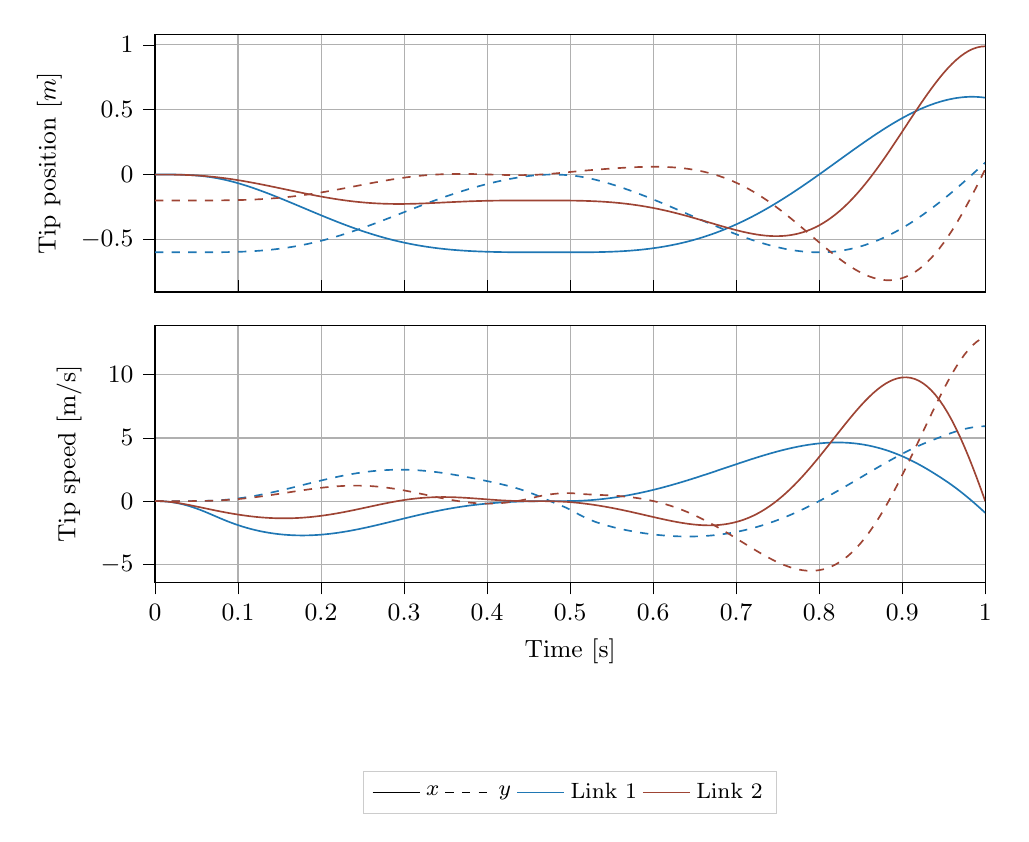
\begin{tikzpicture}

\definecolor{color0}{rgb}{0.12156862745098,0.466666666666667,0.705882352941177}
\definecolor{color1}{rgb}{0.62156862745098,0.266666666666667,0.205882352941177}

\begin{groupplot}[group style={group size=1 by 2,vertical sep=12}]
\nextgroupplot[
ytick align=outside,
xticklabels={},
tick pos=left,
%title={Minimum Mixed Objective - Tip},
x grid style={white!69.0196078431373!black},
xmajorgrids,
xmin=0, xmax=1,
xtick style={color=black},
y grid style={white!69.0196078431373!black},
ylabel={Tip position [$m$]},
ymajorgrids,
ymin=-0.905789645398886, ymax=1.07965007631472,
ytick style={color=black}
]
\addplot [semithick, color0]
table {%
0 0.000477796026439958
0.005 0.000477796026439958
0.01 0.000477796026439958
0.015 0.00041006853654841
0.02 0.000207634109141991
0.025 -0.00019560350227917
0.03 -0.000864684292381848
0.035 -0.00186336559251155
0.04 -0.00325381863989863
0.045 -0.00509621133293122
0.05 -0.00744811874149606
0.055 -0.0103636663988564
0.06 -0.0138922497464608
0.065 -0.0180765788143499
0.07 -0.02294972369488
0.075 -0.0285311842391278
0.08 -0.0348238336290432
0.085 -0.0418150311550916
0.09 -0.0494808641595295
0.095 -0.0577901410653986
0.1 -0.0667071956265104
0.105 -0.0761937710563357
0.11 -0.0862102996700035
0.115 -0.096716772038635
0.12 -0.107673311007187
0.125 -0.119040528238622
0.13 -0.130779722898645
0.135 -0.142852970958714
0.14 -0.155223144131062
0.145 -0.167853888373859
0.15 -0.180709583517588
0.155 -0.193755298459357
0.16 -0.206956750887514
0.165 -0.220280276620865
0.17 -0.23369281112228
0.175 -0.247161884230735
0.18 -0.260655628315419
0.185 -0.274142799618887
0.19 -0.287592812325162
0.195 -0.300975784731617
0.2 -0.314262596741366
0.205 -0.327424957686403
0.21 -0.340435483230617
0.215 -0.353267779796807
0.22 -0.365896534638646
0.225 -0.378297609371749
0.23 -0.390448134525593
0.235 -0.402326602514741
0.24 -0.41391295638046
0.245 -0.425188671736623
0.25 -0.436136829567852
0.255 -0.446742177862637
0.26 -0.456991180501784
0.265 -0.466872052341789
0.27 -0.476374780011312
0.275 -0.485491128551254
0.28 -0.494214634641188
0.285 -0.502540587719016
0.29 -0.510466000753328
0.295 -0.517989572695497
0.3 -0.525111644651273
0.305 -0.531834151523411
0.31 -0.538160570286004
0.315 -0.544095865220312
0.32 -0.549646429503025
0.325 -0.554820021679067
0.33 -0.559625694973294
0.335 -0.564073717251678
0.34 -0.568175479778803
0.345 -0.571943393652956
0.35 -0.575390773758196
0.355 -0.578531711062928
0.36 -0.581380934980298
0.365 -0.583953668236613
0.37 -0.586265477286621
0.375 -0.5883321218046
0.38 -0.590169407175497
0.385 -0.591793044165136
0.39 -0.593218519974288
0.395 -0.594460984610377
0.4 -0.595535156012221
0.405 -0.596455246931125
0.41 -0.597234916674393
0.415 -0.597887251933353
0.42 -0.598424783202909
0.425 -0.598859545362858
0.43 -0.599203186851238
0.435 -0.599467110893425
0.44 -0.599662597488906
0.445 -0.599800841338953
0.45 -0.599892868442443
0.455 -0.599949329506059
0.46 -0.599980187637188
0.465 -0.599994327392647
0.47 -0.599999118859071
0.475 -0.599999979708295
0.48 -0.6
0.485 -0.599999749491242
0.49 -0.599997386492833
0.495 -0.599989008176914
0.5 -0.599967905124127
0.505 -0.599923706853826
0.51 -0.599841444827761
0.515 -0.599700523740698
0.52 -0.599479866238742
0.525 -0.599157477148874
0.53 -0.598711486655913
0.535 -0.598121101388857
0.54 -0.597366277360901
0.545 -0.596427210715572
0.55 -0.595284348084627
0.555 -0.593918390780774
0.56 -0.592310300558431
0.565 -0.590441309135237
0.57 -0.58829293188889
0.575 -0.585846985567363
0.58 -0.583085609685625
0.585 -0.579991291260135
0.59 -0.576546892556764
0.595 -0.572735681562956
0.6 -0.568541364928225
0.605 -0.563948123144589
0.61 -0.558940647759747
0.615 -0.553504180431288
0.62 -0.54762455364091
0.625 -0.541288232894355
0.63 -0.534482360236468
0.635 -0.527194798911938
0.64 -0.51941417900156
0.645 -0.511129943861629
0.65 -0.502332397190666
0.655 -0.493012750543462
0.66 -0.483163171107514
0.665 -0.472776829551624
0.67 -0.461847947750843
0.675 -0.450371846186225
0.68 -0.438344990812155
0.685 -0.425765039178406
0.69 -0.412630885588741
0.695 -0.39894270507277
0.7 -0.38470199594319
0.705 -0.369911620706321
0.71 -0.354575845090329
0.715 -0.338700374952537
0.72 -0.322292390825089
0.725 -0.30536057985676
0.73 -0.287915164908207
0.735 -0.26996793055831
0.74 -0.251532245780638
0.745 -0.232623083051481
0.75 -0.213257033654429
0.755 -0.193452318951108
0.76 -0.173228797393602
0.765 -0.152607967061127
0.77 -0.131612963511956
0.775 -0.110268552751212
0.78 -0.0886011191261832
0.785 -0.0666386479731188
0.79 -0.0444107028531716
0.795 -0.0219483972301776
0.8 0.000715639540647482
0.805 0.0235473020263004
0.81 0.0465110544260477
0.815 0.0695699822518262
0.82 0.0926858500313193
0.825 0.115819165063314
0.83 0.138929247231095
0.835 0.161974304854712
0.84 0.184911516537087
0.845 0.207697118932134
0.85 0.230286500335536
0.855 0.25263429997057
0.86 0.274694512812593
0.865 0.296420599766608
0.87 0.317765602982803
0.875 0.338682266065368
0.88 0.359123158900224
0.885 0.379040806797935
0.89 0.398387823618933
0.895 0.417117048519664
0.9 0.435181685930449
0.905 0.452535448348849
0.91 0.469132701506534
0.915 0.484928611443043
0.92 0.499879292996708
0.925 0.513941959201593
0.93 0.527075071059665
0.935 0.539238487139901
0.94 0.550393612440701
0.945 0.560514543912218
0.95 0.5695764111642
0.955 0.577548410441114
0.96 0.584393575040822
0.965 0.590063032718495
0.97 0.594504905382456
0.975 0.597669556018687
0.98 0.599509915600908
0.985 0.599981814639023
0.99 0.599044317544076
0.995 0.596660057847661
1 0.592795572179525
};
\addplot [semithick, color0,dashed]
table {%
0 -0.599999809759101
0.005 -0.599999809759101
0.01 -0.599999809759101
0.015 -0.599999859869813
0.02 -0.599999964073396
0.025 -0.599999968116057
0.03 -0.599999376933905
0.035 -0.599997106550247
0.04 -0.599991177155347
0.045 -0.599978356801352
0.05 -0.599953769491627
0.055 -0.599910488672079
0.06 -0.599839149603443
0.065 -0.599727635930152
0.07 -0.599560931167407
0.075 -0.599321259030508
0.08 -0.598988564674967
0.085 -0.598541145761508
0.09 -0.597956222546455
0.095 -0.597210431586423
0.1 -0.596280261329894
0.105 -0.595142427702995
0.11 -0.593774186228071
0.115 -0.59215358312386
0.12 -0.590259653116109
0.125 -0.588072574293913
0.13 -0.585573790464151
0.135 -0.582746109972661
0.14 -0.579573787818314
0.145 -0.57604259578418
0.15 -0.572139883616673
0.155 -0.567854633087488
0.16 -0.563177505997961
0.165 -0.558100886696873
0.17 -0.552618919355614
0.175 -0.546727539989996
0.18 -0.540424502985842
0.185 -0.533709401657043
0.19 -0.526583682142643
0.195 -0.519050649749316
0.2 -0.511115466689645
0.205 -0.502785140078798
0.21 -0.494068499054065
0.215 -0.484976159988751
0.22 -0.47552047899058
0.225 -0.46571549119996
0.23 -0.455576836818428
0.235 -0.445121674274513
0.24 -0.434368581437916
0.245 -0.423337446284694
0.25 -0.412049348858243
0.255 -0.400526436728648
0.26 -0.388791796394402
0.265 -0.376869323164098
0.27 -0.364783591968134
0.275 -0.352559731248522
0.28 -0.340223301533679
0.285 -0.327800179522566
0.29 -0.315316447517257
0.295 -0.302798286948154
0.3 -0.290271873683337
0.305 -0.27776327200221
0.31 -0.265298323759203
0.315 -0.252902529544803
0.32 -0.240600919646156
0.325 -0.228417914236252
0.33 -0.216377174225143
0.335 -0.204501446219517
0.34 -0.192812406701766
0.345 -0.181330511654106
0.35 -0.170074858441641
0.355 -0.159063067035061
0.36 -0.148311187849852
0.365 -0.137833643763065
0.37 -0.127643214241458
0.375 -0.117751069858823
0.38 -0.10816686569427
0.385 -0.098898902308173
0.39 -0.089954363760274
0.395 -0.0813396445533221
0.4 -0.0730607825957231
0.405 -0.065124023281203
0.41 -0.0575365475583234
0.415 -0.0503073948399588
0.42 -0.0434485770601431
0.425 -0.0369762752016924
0.43 -0.0309118240697771
0.435 -0.0252820678958445
0.44 -0.0201188760336566
0.445 -0.0154580312162988
0.45 -0.0113378301230114
0.455 -0.00779756533993152
0.46 -0.0048759043104134
0.465 -0.00260904132680093
0.47 -0.001028284171802
0.475 -0.000156045010102346
0.48 -7.34788079488412e-17
0.485 -0.000548279533622229
0.49 -0.00177093245779821
0.495 -0.00363181316734528
0.5 -0.00620586987990541
0.505 -0.0095679650273493
0.51 -0.0137927903973277
0.515 -0.0189547309433017
0.52 -0.0249777896215725
0.525 -0.0317854931784384
0.53 -0.0393008364575904
0.535 -0.0474462651151831
0.54 -0.0561563057187641
0.545 -0.0653802899813259
0.55 -0.075076926718271
0.555 -0.0852111793861326
0.56 -0.0957523255716584
0.565 -0.106672679101389
0.57 -0.117946709532629
0.575 -0.129550412973616
0.58 -0.14146084892133
0.585 -0.153655790852154
0.59 -0.166113457260811
0.595 -0.17881230121168
0.6 -0.191730843542584
0.605 -0.204847539408447
0.61 -0.218140670856938
0.615 -0.231588260162487
0.62 -0.245168000052197
0.625 -0.25885719794919
0.63 -0.272632732070186
0.635 -0.28647101773164
0.64 -0.300347982600408
0.645 -0.314239049909473
0.65 -0.328119128873461
0.655 -0.341962611701294
0.66 -0.355743376727285
0.665 -0.369434797277022
0.67 -0.383009755957122
0.675 -0.396440664113573
0.68 -0.40969948624558
0.685 -0.422757769193436
0.69 -0.435586675942058
0.695 -0.448157023898121
0.7 -0.460439327509419
0.705 -0.472403845101225
0.71 -0.484020629806705
0.715 -0.495259584467591
0.72 -0.506090520377776
0.725 -0.516483219736656
0.73 -0.526407501671357
0.735 -0.535833291677611
0.74 -0.544730694318347
0.745 -0.553070069007195
0.75 -0.560822108691262
0.755 -0.567957921233993
0.76 -0.57444911328469
0.765 -0.580267876406638
0.77 -0.585387075220832
0.775 -0.589780337307165
0.78 -0.593422144589826
0.785 -0.596287925918607
0.79 -0.598354150543044
0.795 -0.599598422161889
0.8 -0.599999573216555
0.805 -0.599537759083848
0.81 -0.598194551810845
0.815 -0.595953033023141
0.82 -0.59279788562711
0.825 -0.588715483917348
0.83 -0.583693981692292
0.835 -0.57772339797418
0.84 -0.570795699924198
0.845 -0.562904882539929
0.85 -0.554047044720221
0.855 -0.544220461282356
0.86 -0.533425650518094
0.865 -0.521665436878853
0.87 -0.508945008385951
0.875 -0.495271968369731
0.88 -0.480656381151363
0.885 -0.465110811293363
0.89 -0.448650356059337
0.895 -0.431292670740234
0.9 -0.413057986523359
0.905 -0.393969120601737
0.91 -0.374051478244882
0.915 -0.353333046577761
0.92 -0.331844379842587
0.925 -0.309618575947937
0.93 -0.286691244141583
0.935 -0.263100463677035
0.94 -0.23888673337897
0.945 -0.214064116710106
0.95 -0.188633803559465
0.955 -0.162597151257157
0.96 -0.135956424824304
0.965 -0.108745654713429
0.97 -0.0810180071107489
0.975 -0.0528308793077023
0.98 -0.0242458469885549
0.985 0.00467141332633128
0.99 0.0338512277200049
0.995 0.0632200551188162
1 0.0927006451129062
};
\addplot [semithick, color1]
table {%
0 -0.000477795218472657
0.005 -0.000477795218472657
0.01 -0.000477795218472657
0.015 -0.000541403986433626
0.02 -0.000728670160688234
0.025 -0.0010946262120739
0.03 -0.00168732837194933
0.035 -0.00254570854158072
0.04 -0.00369849541816139
0.045 -0.00516540076188399
0.05 -0.00695954562278916
0.055 -0.00908955033312515
0.06 -0.0115608459812914
0.065 -0.0143762663158506
0.07 -0.0175359714482617
0.075 -0.0210367853126378
0.08 -0.0248715627276789
0.085 -0.0290296490115531
0.09 -0.0334980706344668
0.095 -0.0382623766289466
0.1 -0.043306928679478
0.105 -0.0486148742397135
0.11 -0.0541680362044324
0.115 -0.0599468564378339
0.12 -0.0659304390552466
0.125 -0.0720966804923586
0.13 -0.0784224505307817
0.135 -0.0848837900834984
0.14 -0.0914561029115525
0.145 -0.0981143298795708
0.15 -0.10483310231253
0.155 -0.111586875464983
0.16 -0.118350045159151
0.165 -0.125097051349501
0.17 -0.131802472430765
0.175 -0.138441113906313
0.18 -0.144988094751229
0.185 -0.151418934505042
0.19 -0.157709643825268
0.195 -0.163836820915084
0.2 -0.169777755888981
0.205 -0.175510544741202
0.21 -0.181014214117606
0.215 -0.186268857552147
0.22 -0.191255783212067
0.225 -0.195957672508474
0.23 -0.200358748189651
0.235 -0.204444949770953
0.24 -0.208204113400863
0.245 -0.211626152548606
0.25 -0.214703235244871
0.255 -0.217429953013694
0.26 -0.219803476077665
0.265 -0.221823688858652
0.27 -0.223493299192005
0.275 -0.224817914020633
0.28 -0.225806073724563
0.285 -0.226469236904571
0.29 -0.226821707774023
0.295 -0.226880499817523
0.3 -0.226665132447769
0.305 -0.226197362051006
0.31 -0.2255008544727
0.315 -0.224600811521901
0.32 -0.223523568157922
0.325 -0.222296178707285
0.33 -0.22094600945932
0.335 -0.219500351681119
0.34 -0.217986064261173
0.345 -0.216429249758551
0.35 -0.214854962490523
0.355 -0.213286943216942
0.36 -0.211747372621017
0.365 -0.210256635615841
0.37 -0.208833090714939
0.375 -0.207492843011879
0.38 -0.206249524820591
0.385 -0.20511409334466
0.39 -0.204094658464938
0.395 -0.203196354996848
0.4 -0.202421272541899
0.405 -0.201768453104871
0.41 -0.201233963258244
0.415 -0.20081104522962
0.42 -0.200490351127546
0.425 -0.200260267633699
0.43 -0.200107345057517
0.435 -0.200016851597515
0.44 -0.199973473257647
0.445 -0.199962167934116
0.45 -0.199969167112868
0.455 -0.199983109835353
0.46 -0.199996288175648
0.465 -0.20000598321999
0.47 -0.200014991129221
0.475 -0.200032277719453
0.48 -0.200071592441246
0.485 -0.200149896274425
0.49 -0.200285751820929
0.495 -0.200498038182391
0.5 -0.200808555582433
0.505 -0.201240630488141
0.51 -0.201818722716633
0.515 -0.202567969898359
0.52 -0.20350889457707
0.525 -0.204660872811021
0.53 -0.206042225910189
0.535 -0.207670287211928
0.54 -0.209561868302229
0.545 -0.211733370310918
0.55 -0.214200562358669
0.555 -0.216978388999283
0.56 -0.220080789671
0.565 -0.223520522555436
0.57 -0.227308989213006
0.575 -0.231456058294306
0.58 -0.235969887678393
0.585 -0.240856745020331
0.59 -0.246120827104022
0.595 -0.251764078689346
0.6 -0.257786011764772
0.605 -0.26418352629466
0.61 -0.270950733699718
0.615 -0.278078784437894
0.62 -0.28555570116658
0.625 -0.29336621906798
0.63 -0.301491635009407
0.635 -0.309909667289692
0.64 -0.318594327791766
0.645 -0.327515808419656
0.65 -0.336640383744754
0.655 -0.345930331820794
0.66 -0.355343875148361
0.665 -0.364835143777115
0.67 -0.374354162526206
0.675 -0.383846864279472
0.68 -0.393255131270909
0.685 -0.402516866216594
0.69 -0.41156609507058
0.695 -0.420333103083427
0.7 -0.428744605721971
0.705 -0.436723955866898
0.71 -0.444191388539872
0.715 -0.451064304223862
0.72 -0.457257591628251
0.725 -0.46268399051415
0.73 -0.467254494934731
0.735 -0.470878796960488
0.74 -0.473465770650265
0.745 -0.474923995696171
0.75 -0.475162319814827
0.755 -0.474090458579744
0.76 -0.471619630991285
0.765 -0.467663228663209
0.77 -0.462137516070246
0.775 -0.454962358851585
0.78 -0.446061976703531
0.785 -0.435365716923635
0.79 -0.422808844192017
0.795 -0.408333341697082
0.8 -0.391888718236746
0.805 -0.37343281545724
0.81 -0.352932608934785
0.815 -0.330364996366305
0.82 -0.305717565719879
0.825 -0.278989335810095
0.83 -0.250191461414446
0.835 -0.219347894741394
0.84 -0.186495994805846
0.845 -0.151687076071027
0.85 -0.114986887584485
0.855 -0.0764760137779825
0.86 -0.0362501881236845
0.865 0.00557948905008587
0.87 0.0488864370741001
0.875 0.0935285939667874
0.88 0.1393485357417
0.885 0.186173723228664
0.89 0.233816882993618
0.895 0.282076528169496
0.9 0.330737624112102
0.905 0.379572402769372
0.91 0.428341328499475
0.915 0.476794216794559
0.92 0.524671505965806
0.925 0.571705680327155
0.93 0.617622841786785
0.935 0.662144425026879
0.94 0.704989049634976
0.945 0.745872804535964
0.95 0.784509188370044
0.955 0.820611929174799
0.96 0.853898167817772
0.965 0.884095685161213
0.97 0.91094604674972
0.975 0.934205541518811
0.98 0.953647305295577
0.985 0.969063385566799
0.99 0.980266731505675
0.995 0.987093093443344
1 0.989402816236824
};
\addplot [semithick, color1,dashed]
table {%
0 -0.200000951204014
0.005 -0.200000951204014
0.01 -0.200000951204014
0.015 -0.200000991496366
0.02 -0.200001059907004
0.025 -0.200000978419624
0.03 -0.200000222863902
0.035 -0.199997688540546
0.04 -0.199991424327219
0.045 -0.199978362785323
0.05 -0.199954067871354
0.055 -0.199912517891913
0.06 -0.199845943965543
0.065 -0.199744751687071
0.07 -0.199597568737031
0.075 -0.199391472712046
0.08 -0.199112393462045
0.085 -0.198745530473592
0.09 -0.198275662209659
0.095 -0.197687382919497
0.1 -0.196965313567094
0.105 -0.196094304727359
0.11 -0.195059635011285
0.115 -0.193847201921261
0.12 -0.192443699889992
0.125 -0.190836781396576
0.13 -0.189015199546999
0.135 -0.186968932676324
0.14 -0.184689292738918
0.145 -0.182169019644549
0.15 -0.179402363636803
0.155 -0.176385157569131
0.16 -0.17311488064151
0.165 -0.169590714851989
0.17 -0.165813595088576
0.175 -0.161786253427923
0.18 -0.157513257813834
0.185 -0.153001044864709
0.19 -0.148257946115568
0.195 -0.143294206553291
0.2 -0.138121993872947
0.205 -0.132755396491185
0.21 -0.127210408023763
0.215 -0.121504895692491
0.22 -0.115658549993971
0.225 -0.109692812955024
0.23 -0.103630782425962
0.235 -0.0974970901217418
0.24 -0.0913177515015997
0.245 -0.0851199860641016
0.25 -0.0789320072123822
0.255 -0.0727827815119105
0.26 -0.0667017579423922
0.265 -0.0607185686904826
0.27 -0.0548627042263844
0.275 -0.049163166953089
0.28 -0.0436481096738975
0.285 -0.0383444674360916
0.29 -0.033277593704045
0.295 -0.0284709137457588
0.3 -0.0239456088246794
0.305 -0.0197203435561844
0.31 -0.0158110453108948
0.315 -0.0122307392114753
0.32 -0.0089894361051136
0.325 -0.00609406518879158
0.33 -0.00354843880589661
0.335 -0.00135323495646347
0.34 0.000494016521624174
0.345 0.00199895540187103
0.35 0.00317042661270375
0.355 0.00402052981370821
0.36 0.00456467544317057
0.365 0.00482163237640992
0.37 0.00481354688006511
0.375 0.00456591068206563
0.38 0.00410745876415319
0.385 0.00346998452945931
0.39 0.00268806930391335
0.395 0.00179873174419411
0.4 0.0008410077945087
0.405 -0.000144528214283887
0.41 -0.00111629504646744
0.415 -0.00203228666012457
0.42 -0.00285069818872601
0.425 -0.0035305610697885
0.43 -0.0040322953729819
0.435 -0.00431804279497177
0.44 -0.00435169584033187
0.445 -0.00409866284213442
0.45 -0.00352546077349781
0.455 -0.00259918844664379
0.46 -0.00128700872257545
0.465 0.000444567360645285
0.47 0.00253507999577519
0.475 0.00492700188766781
0.48 0.00756761703041431
0.485 0.0104105015341072
0.49 0.0134148868455636
0.495 0.0165415577169321
0.5 0.0197134988132443
0.505 0.022863572395251
0.51 0.0259301586780875
0.515 0.0288546267041503
0.52 0.0316524991054945
0.525 0.0343388530633444
0.53 0.0369281059816609
0.535 0.0394338920472729
0.54 0.0418627756616206
0.545 0.0442128172595875
0.55 0.0464761409385018
0.555 0.0486403617218038
0.56 0.0506894417780427
0.565 0.0526042381705765
0.57 0.0543628756046313
0.575 0.0559410171964677
0.58 0.0573120756317849
0.585 0.0584473905165428
0.59 0.0593163882996653
0.595 0.0598867355453751
0.6 0.0601244928715119
0.605 0.0599942746530783
0.61 0.0594594181194483
0.615 0.0584821644620894
0.62 0.0570238538465938
0.625 0.0550451356838594
0.63 0.0525061950950609
0.635 0.0493669961618194
0.64 0.0455875422594655
0.645 0.0411281535096061
0.65 0.0359497611463255
0.655 0.0300142183603235
0.66 0.0232846269617649
0.665 0.0157256789821042
0.67 0.00730401211552084
0.675 -0.00201142231942553
0.68 -0.0122489804381891
0.685 -0.023433937630708
0.69 -0.0355880931681281
0.695 -0.0487293697817016
0.7 -0.0628714106400192
0.705 -0.0780231763680954
0.71 -0.0941885449647266
0.715 -0.111365917681189
0.72 -0.129547834122735
0.725 -0.148720600022354
0.73 -0.168863931311551
0.735 -0.189950618272991
0.74 -0.211946213702224
0.745 -0.234808749127524
0.75 -0.258488483235475
0.755 -0.282927686722322
0.76 -0.308060467834325
0.765 -0.333812642871532
0.77 -0.360101655905373
0.775 -0.3868365518984
0.78 -0.413918007311413
0.785 -0.441238422136231
0.79 -0.468682077098885
0.795 -0.496125359535391
0.8 -0.523437061148309
0.805 -0.550478750504846
0.81 -0.5771052227348
0.815 -0.603165028427652
0.82 -0.628501083211886
0.825 -0.652951358925721
0.83 -0.676349656657141
0.835 -0.698526461243236
0.84 -0.719309876076002
0.845 -0.738526636266312
0.85 -0.756003197372798
0.855 -0.771566896012107
0.86 -0.785047177736353
0.865 -0.796276886598598
0.87 -0.80509360983502
0.875 -0.811341070081021
0.88 -0.814870556517294
0.885 -0.815542385320995
0.89 -0.813227378788005
0.895 -0.807808351507391
0.9 -0.799181591021822
0.905 -0.78725831951237
0.91 -0.771966122217932
0.915 -0.753250327554344
0.92 -0.731075323252657
0.925 -0.70542579230677
0.93 -0.676307852124802
0.935 -0.643750080033235
0.94 -0.607804408204549
0.945 -0.568524714264389
0.95 -0.525982141753953
0.955 -0.480276432704342
0.96 -0.43153598174956
0.965 -0.379937098711022
0.97 -0.32569126688832
0.975 -0.269033401178889
0.98 -0.21022087009716
0.985 -0.149532328526726
0.99 -0.0872663642858299
0.995 -0.02373996279482
1 0.0407132046943376
};

\nextgroupplot[
legend cell align={left},
legend entries={{\footnotesize{$x$}},{\footnotesize{$y$}},{\footnotesize{Link 1}},{\footnotesize{Link 2}}},
legend style={at={(0.5,-0.9)}, anchor=south, draw=white!80.0!black},
legend columns=4,
tick align=outside,
tick pos=left,
x grid style={white!69.0196078431373!black},
xlabel={Time [s]},
xmajorgrids,
xmin=0, xmax=1,
xtick style={color=black},
y grid style={white!69.0196078431373!black},
ylabel={Tip speed [m/s]},
ymajorgrids,
ymin=-6.44191173366682, ymax=13.9258052172039,
ytick style={color=black}
]
\addlegendimage{no markers, black}
\addlegendimage{no markers, black,dashed}
\addlegendimage{no markers, color0}
\addlegendimage{no markers, color1}
\addplot [semithick, color0]
table {%
0 0
0.005 0
0.01 -0.0135454973982793
0.015 -0.0404868815814855
0.02 -0.0806475189770636
0.025 -0.133816210078329
0.03 -0.199736591811623
0.035 -0.278091859122904
0.04 -0.368482185847335
0.045 -0.470390517733257
0.05 -0.583129417391296
0.055 -0.705756597641375
0.06 -0.836940215490406
0.065 -0.974759087802198
0.07 -1.11650720374219
0.075 -1.2588677202522
0.08 -1.39874602221514
0.085 -1.53389512151064
0.09 -1.6628655969479
0.095 -1.78476763908633
0.1 -1.89908692845062
0.105 -2.00556373774727
0.11 -2.10411090350169
0.115 -2.19475490528686
0.12 -2.27759248833257
0.125 -2.35275920285524
0.13 -2.42040762504253
0.135 -2.48069336571156
0.14 -2.53376705381091
0.145 -2.57977062072602
0.15 -2.61883646761303
0.155 -2.65108842126283
0.16 -2.67664370458821
0.165 -2.69561541815741
0.17 -2.70811523079768
0.175 -2.71425611238669
0.18 -2.71415502275469
0.185 -2.70793551176721
0.19 -2.69573020034906
0.195 -2.67768311095895
0.2 -2.65395180673661
0.205 -2.62470928704408
0.21 -2.59014557767504
0.215 -2.55046894963538
0.22 -2.50590670299038
0.225 -2.45670546254507
0.23 -2.40313094957754
0.235 -2.34546721686528
0.24 -2.28401536041609
0.245 -2.21909174795613
0.25 -2.15102582900914
0.255 -2.08015761280094
0.26 -2.00683491757311
0.265 -1.9314105079149
0.27 -1.85423924475035
0.275 -1.77567537387679
0.28 -1.69607007047903
0.285 -1.61576933547292
0.29 -1.53511230259968
0.295 -1.45442996339531
0.3 -1.37404425502929
0.305 -1.29426739263892
0.31 -1.2154012762667
0.315 -1.1377367775664
0.32 -1.06155272502547
0.325 -0.987114462062306
0.33 -0.914671940669376
0.335 -0.844457412576159
0.34 -0.776682863608154
0.345 -0.711537385290604
0.35 -0.649184686569202
0.355 -0.589760928757353
0.36 -0.533373036176236
0.365 -0.480097607522909
0.37 -0.429980532993031
0.375 -0.383037403785939
0.38 -0.339254772392136
0.385 -0.298592274299079
0.39 -0.260985557963341
0.395 -0.226349918949551
0.4 -0.194584545732153
0.405 -0.165577402292787
0.41 -0.139211011988061
0.415 -0.115369724101818
0.42 -0.0939491347593246
0.425 -0.074867164393648
0.43 -0.0580726003316771
0.435 -0.0435433663639033
0.44 -0.031270811299267
0.445 -0.021235402400601
0.45 -0.0133813610776175
0.455 -0.00759437864721636
0.46 -0.00368440952914194
0.465 -0.00137476029467151
0.47 -0.000298970079932998
0.475 -8.11765979774801e-06
0.48 1.34294379001572e-17
0.485 0.000223452314335887
0.49 0.0010985095902982
0.495 0.00311627146587445
0.5 0.00695551838066261
0.505 0.0134769089594749
0.51 0.0237414367765965
0.515 0.0380808417664362
0.52 0.0567442887956272
0.525 0.0797669079210856
0.53 0.106988135277387
0.535 0.138270496523901
0.54 0.173555837834096
0.545 0.212788044773694
0.55 0.255912672437086
0.555 0.302875782135758
0.56 0.353622696827821
0.565 0.408096861281251
0.57 0.466238840753168
0.575 0.527985448513624
0.58 0.593268982761938
0.585 0.662016554028307
0.59 0.734149487412487
0.595 0.809582787518476
0.6 0.888224656980803
0.605 0.969976061916127
0.61 1.0547303395315
0.615 1.14237284457881
0.62 1.23278063246074
0.625 1.32582217764732
0.63 1.4213571267162
0.635 1.51923608583132
0.64 1.61930044285844
0.645 1.72138222460911
0.65 1.82530398992525
0.655 1.93087875947964
0.66 2.0379099832839
0.665 2.1461915469728
0.67 2.25550781797772
0.675 2.36563373271776
0.68 2.47633492592755
0.685 2.58736790320834
0.69 2.69848025783647
0.695 2.80941093279148
0.7 2.91989052887616
0.705 3.02964165969495
0.71 3.13837935413402
0.715 3.24581150684922
0.72 3.35163937711555
0.725 3.45555813622564
0.73 3.55725746344535
0.735 3.65642219034253
0.74 3.75273299310086
0.745 3.84586713221558
0.75 3.93549923874235
0.755 4.02130214603526
0.76 4.1029477656665
0.765 4.18010800596887
0.77 4.25245573138471
0.775 4.31966576054184
0.78 4.38141590071042
0.785 4.43738801602505
0.79 4.48726912658586
0.795 4.53075253528224
0.8 4.56753897891474
0.805 4.5973377999261
0.81 4.61986813479371
0.815 4.63486011488408
0.82 4.64205607532755
0.825 4.64121176724052
0.83 4.63209756840415
0.835 4.61449968730594
0.84 4.5882213552648
0.845 4.55308400119371
0.85 4.50892840340885
0.855 4.45561581277224
0.86 4.39302904135763
0.865 4.32107351075988
0.87 4.23967825412675
0.875 4.1487968659817
0.88 4.04840839392764
0.885 3.93851816637705
0.89 3.81915855054355
0.895 3.69038963505643
0.9 3.55229983172222
0.905 3.40500639115817
0.91 3.24865582726135
0.915 3.08342424575384
0.92 2.90951757236037
0.925 2.72717167652899
0.93 2.53665238699873
0.935 2.33825539595994
0.94 2.13476054088627
0.945 1.92649942502305
0.95 1.71229827000022
0.955 1.49093413794346
0.96 1.2597544283416
0.965 1.01799502854082
0.97 0.766075638916732
0.975 0.504480919737248
0.98 0.233761573984782
0.985 -0.0454649217376173
0.99 -0.332513966744763
0.995 -0.626633893748321
1 -0.927006451129062
};
\addplot [semithick, color0,dashed]
table {%
0 0
0.005 0
0.01 -1.07866448085194e-05
0.015 -2.76706669283738e-05
0.02 -2.79086279332944e-05
0.025 4.36248679066317e-05
0.03 0.00028784878817036
0.035 0.000863648834619496
0.04 0.00199831972607527
0.045 0.00399549327105028
0.05 0.00723925302789584
0.055 0.0121921954605884
0.06 0.0193835005670039
0.065 0.0293805194558559
0.07 0.042737160640762
0.075 0.0599294390412706
0.08 0.0813199143348216
0.085 0.107160339349782
0.09 0.137602091283099
0.095 0.172706249215661
0.1 0.212455067631052
0.105 0.25676452754779
0.11 0.305496661419578
0.115 0.35847053180949
0.12 0.415471264297352
0.125 0.476257031136754
0.13 0.540564218651121
0.135 0.608111167565052
0.14 0.678600890610875
0.145 0.751723106885905
0.15 0.827155842329103
0.155 0.904566764756477
0.16 0.983614364006754
0.165 1.06394905317127
0.17 1.14521424975123
0.175 1.22704748883614
0.18 1.30908161804815
0.185 1.39094612176291
0.19 1.47226861727601
0.195 1.55267655665723
0.2 1.63179915453023
0.205 1.70926954427259
0.21 1.78472714423543
0.215 1.85782019326328
0.22 1.92820839325008
0.225 1.99556557806724
0.23 2.05958231510622
0.235 2.11996833946386
0.24 2.17645472220538
0.245 2.22879568310299
0.25 2.27676997423276
0.255 2.32018178333087
0.26 2.35886113482599
0.265 2.39266380233367
0.27 2.4214707891342
0.275 2.44518748114325
0.28 2.46374262559047
0.285 2.47708732999954
0.29 2.48519429920447
0.295 2.48805752122257
0.3 2.48569256616709
0.305 2.47813757249756
0.31 2.46545486866965
0.315 2.44773303571603
0.32 2.42508908900914
0.325 2.3976703800678
0.33 2.36565581514186
0.335 2.32925605455747
0.34 2.28871246521552
0.345 2.24429470331142
0.35 2.19629686915306
0.355 2.14503219126818
0.36 2.09082618082295
0.365 2.03400818095291
0.37 1.97490124247622
0.375 1.91381028444236
0.38 1.85100850079204
0.385 1.78672186290829
0.39 1.72111123860841
0.395 1.65425109027887
0.4 1.58610315525074
0.405 1.51648355545109
0.41 1.44502374009439
0.415 1.37113216693058
0.42 1.29397771813392
0.425 1.2125319758907
0.43 1.1256950450071
0.435 1.03246364736776
0.44 0.932056835477987
0.445 0.823973767928603
0.45 0.708017583031476
0.455 0.58431602414153
0.46 0.453366715155943
0.465 0.31614998576467
0.47 0.174447676473196
0.475 0.0312127616944185
0.48 -0.10965968236317
0.485 -0.244530981740323
0.49 -0.372178442104838
0.495 -0.514819606589711
0.5 -0.672442038369343
0.505 -0.845019516353691
0.51 -1.03250301991972
0.515 -1.2048232612813
0.52 -1.36189227199014
0.525 -1.50360855002824
0.53 -1.6298641784785
0.535 -1.74307717308595
0.54 -1.84621127465946
0.545 -1.94114434264889
0.55 -2.02912952137706
0.555 -2.11103165603893
0.56 -2.18745983026406
0.565 -2.25884684868428
0.57 -2.32549950459856
0.575 -2.38763178237135
0.58 -2.44538760483259
0.585 -2.49885691829154
0.59 -2.5480873893031
0.595 -2.5930931286552
0.6 -2.63386135225869
0.605 -2.67035758004435
0.61 -2.70252977986037
0.615 -2.73031173791761
0.62 -2.7536258542907
0.625 -2.77238550581749
0.63 -2.78649708000075
0.635 -2.79586175631876
0.64 -2.80037709193867
0.645 -2.79993845476025
0.65 -2.79444033637686
0.655 -2.78377756983718
0.66 -2.76784647127792
0.665 -2.74654592005702
0.67 -2.71977838858394
0.675 -2.68745093035988
0.68 -2.64947613261802
0.685 -2.60577303825822
0.69 -2.5562680404001
0.695 -2.50089575176141
0.7 -2.43959985014811
0.705 -2.37233390057824
0.71 -2.29906215392205
0.715 -2.21976032140177
0.72 -2.13441632383817
0.725 -2.04303101414335
0.73 -1.94561887122998
0.735 -1.8422086632276
0.74 -1.73284407766108
0.745 -1.61758431604931
0.75 -1.49650465022142
0.755 -1.36969693751853
0.76 -1.23727009195144
0.765 -1.0993505083156
0.77 -0.956082436223607
0.775 -0.807628301002239
0.78 -0.654168968413743
0.785 -0.495903950200716
0.79 -0.333051547519397
0.795 -0.165848929417563
0.8 0.00544785636969154
0.805 0.180563942890288
0.81 0.359205776127662
0.815 0.541061322058347
0.82 0.725800350619718
0.825 0.913074798350801
0.83 1.10251921120309
0.835 1.29375126872925
0.84 1.48637239054627
0.845 1.67996842563689
0.85 1.87411042470023
0.855 2.06835549539087
0.86 2.26224773989637
0.865 2.45531927389795
0.87 2.64709132554066
0.875 2.83707541260769
0.88 3.02477459565368
0.885 3.20968480440305
0.89 3.39129623426723
0.895 3.56909480937929
0.9 3.74256370809066
0.905 3.91118494642411
0.91 4.07444101453412
0.915 4.23181656079302
0.92 4.3828001177025
0.925 4.52688586343116
0.93 4.66357541240688
0.935 4.7923796280797
0.94 4.91847558537418
0.945 5.044427637661
0.95 5.17025413826184
0.955 5.29582858484263
0.96 5.41491433746829
0.965 5.52372630810937
0.97 5.62141357793992
0.975 5.70713361712497
0.98 5.78005716016048
0.985 5.83937329903964
0.99 5.88429477152392
0.995 5.91406341849104
1 5.92795572179526
};
\addplot [semithick, color1]
table {%
0 0
0.005 0
0.01 -0.0127217530222582
0.015 -0.0374532310872467
0.02 -0.0731912077725636
0.025 -0.118540487217979
0.03 -0.1716763752574
0.035 -0.230558646253762
0.04 -0.293384744140728
0.045 -0.358837985504424
0.05 -0.426020538567339
0.055 -0.494297921325874
0.06 -0.563155203685649
0.065 -0.632063299340569
0.07 -0.700361338975957
0.075 -0.767261920065333
0.08 -0.832069065306444
0.085 -0.894324225421868
0.09 -0.95373633263184
0.095 -1.0100714444826
0.1 -1.06308927642788
0.105 -1.11252646881293
0.11 -1.1581073466116
0.115 -1.19956388953407
0.12 -1.23665313292426
0.125 -1.26916741658771
0.13 -1.29693779973296
0.135 -1.31983290991108
0.14 -1.3377555104751
0.145 -1.35063837665565
0.15 -1.3584403700184
0.155 -1.36114312069894
0.16 -1.35874845820465
0.165 -1.35127660343384
0.17 -1.33876508296772
0.175 -1.32126831051424
0.18 -1.29885777731269
0.185 -1.27162279266579
0.19 -1.2396717130542
0.195 -1.20313359196977
0.2 -1.16216017251403
0.205 -1.11692813149145
0.21 -1.06764146825725
0.215 -1.01453391553515
0.22 -0.9578712348215
0.225 -0.897953248064902
0.23 -0.835115452028264
0.235 -0.769730063198671
0.24 -0.702206348901327
0.245 -0.63299011210708
0.25 -0.562562209268338
0.255 -0.491435987495254
0.26 -0.420153525582966
0.265 -0.349280552715073
0.27 -0.279399906439079
0.275 -0.211103395948435
0.28 -0.144981987465395
0.285 -0.0816143600355939
0.29 -0.0215541138402937
0.295 0.03468376827067
0.3 0.0866362775750025
0.305 0.133904411226118
0.31 0.176162747968475
0.315 0.213165715083181
0.32 0.244750171301666
0.325 0.270834472186695
0.33 0.291414657177997
0.335 0.306558717108216
0.34 0.316400037564319
0.345 0.321131071489284
0.35 0.320998093057741
0.355 0.316297548279526
0.36 0.307374077604357
0.365 0.294619796261645
0.37 0.278473974301255
0.375 0.259421989459707
0.38 0.237992440076711
0.385 0.214751614818196
0.39 0.190295016362692
0.395 0.165236158600079
0.4 0.140193236331803
0.405 0.115774389630959
0.41 0.0925621200095679
0.415 0.0710969909314482
0.42 0.0518600939641037
0.425 0.0352530034706262
0.43 0.0215736668019622
0.435 0.0109879224684422
0.44 0.00349874109333075
0.445 -0.0010837145276648
0.45 -0.0031692060288338
0.455 -0.00341081079817551
0.46 -0.00272383194729906
0.465 -0.00215308385283936
0.47 -0.00300672135762586
0.475 -0.00632347888413465
0.48 -0.0128350434197458
0.485 -0.0229506278451239
0.49 -0.0368088112324695
0.495 -0.0549387456439134
0.5 -0.0776664814330105
0.505 -0.105244500383271
0.51 -0.137839543869448
0.515 -0.174605470915602
0.52 -0.215310066662299
0.525 -0.259741269955738
0.53 -0.307702178510724
0.535 -0.359090977515277
0.54 -0.413832162936649
0.545 -0.471808957097299
0.55 -0.532867865273748
0.555 -0.596820499063077
0.56 -0.663444147672212
0.565 -0.732481739158231
0.57 -0.803641513101308
0.575 -0.876596585321637
0.58 -0.950984516450684
0.585 -1.02640695970326
0.59 -1.10242944255922
0.595 -1.17858132470806
0.6 -1.25435596681186
0.605 -1.32921113944308
0.61 -1.40256969786394
0.615 -1.47382054550256
0.62 -1.54231990666397
0.625 -1.60739292695184
0.63 -1.66833561791468
0.635 -1.724417160465
0.64 -1.77488257958075
0.645 -1.81895580063796
0.65 -1.85584309540573
0.655 -1.88473692323777
0.66 -1.90482017030014
0.665 -1.9152707867733
0.67 -1.91526681885112
0.675 -1.9039918290282
0.68 -1.88064069462126
0.685 -1.84442577071479
0.69 -1.79458339976366
0.695 -1.73038074593714
0.7 -1.65112292796386
0.705 -1.55616041975334
0.71 -1.44489668344813
0.715 -1.31679599482523
0.72 -1.17139141614541
0.725 -1.00829286667571
0.73 -0.827195236220312
0.735 -0.627886482127652
0.74 -0.41025564544221
0.745 -0.174300717185394
0.75 0.0798637187651123
0.755 0.351999144017552
0.76 0.641736147052121
0.765 0.948567933123021
0.77 1.27184439137671
0.775 1.61076681061969
0.78 1.96438333733103
0.785 2.33158527102641
0.79 2.71110429285938
0.795 3.10151072330949
0.8 3.50121290387097
0.805 3.90845779573526
0.81 4.32133288547397
0.815 4.73776948359344
0.82 5.15554749647155
0.825 5.57230174552948
0.83 5.98552989947035
0.835 6.39260207597608
0.84 6.79077215834691
0.845 7.17719086016159
0.85 7.54892055710959
0.855 7.9029518896989
0.86 8.23622212358891
0.865 8.54563523587659
0.87 8.82808367583602
0.875 9.08047172746397
0.88 9.29974037883132
0.885 9.4828935798268
0.89 9.62702574557997
0.895 9.729350337873
0.9 9.78722933143569
0.905 9.79820334644026
0.91 9.7600222030802
0.915 9.67067562917079
0.92 9.52842382762256
0.925 9.33182758781259
0.93 9.07977760374318
0.935 8.77152264288054
0.94 8.40650829254497
0.945 7.98402270640256
0.95 7.50382880432197
0.955 6.96632672369135
0.96 6.37326372297498
0.965 5.72711544803901
0.97 5.03061640566903
0.975 4.28693088446748
0.98 3.49964285295583
0.985 2.67274265165305
0.99 1.81061050943856
0.995 0.917996929153323
1 4.06327671509388e-09
};
\addplot [semithick, color1,dashed]
table {%
0 0
0.005 0
0.01 -8.8187319084296e-06
0.015 -2.04545587895271e-05
0.02 -1.04551400731074e-05
0.025 7.79580090238312e-05
0.03 0.000345557837764182
0.035 0.000944733834215861
0.04 0.00208180499874797
0.045 0.00401478891134681
0.05 0.00704735494749069
0.055 0.0115186348017522
0.06 0.0177877149427191
0.065 0.0262101800258892
0.07 0.0371043681854498
0.075 0.0507170970072043
0.08 0.0672162417613611
0.085 0.0867069926854081
0.09 0.109244778621726
0.095 0.13484088738356
0.1 0.163464744744254
0.105 0.195045197784542
0.11 0.2294721092262
0.115 0.266598818518277
0.12 0.306245382654926
0.125 0.348202186273388
0.13 0.392233512954476
0.135 0.438080823236237
0.14 0.485465636294119
0.145 0.534092005879594
0.15 0.583648624544132
0.155 0.633810606933467
0.16 0.684241010380768
0.165 0.734592157223739
0.17 0.784506830291435
0.175 0.833619420299576
0.18 0.881557110203181
0.185 0.927941185686728
0.19 0.972388561964401
0.195 1.01451361416618
0.2 1.0539303912302
0.205 1.09025528105463
0.21 1.12311017765445
0.215 1.15212617965487
0.22 1.17694782464862
0.225 1.19723783733196
0.23 1.21268234286784
0.235 1.22299647247902
0.24 1.22793026699911
0.245 1.22727476570496
0.25 1.22086814987071
0.255 1.20860178852196
0.26 1.19042600150944
0.265 1.16635530598079
0.27 1.13647284392794
0.275 1.10093360734532
0.28 1.05996600622492
0.285 1.01387130508602
0.29 0.963020540059861
0.295 0.907848762706453
0.3 0.84884683249278
0.305 0.786551418298318
0.31 0.721534236485856
0.315 0.654391722915606
0.32 0.585736256324093
0.325 0.5161897576743
0.33 0.446380070459546
0.335 0.37694006237883
0.34 0.308508931929175
0.345 0.241734786270035
0.35 0.177277214903865
0.355 0.11580837909592
0.36 0.0580111633577993
0.365 0.00457328903275611
0.37 -0.0438230053575686
0.375 -0.0865151887284723
0.38 -0.122877184735326
0.385 -0.152336796279943
0.39 -0.174392084196546
0.395 -0.188625670339895
0.4 -0.19471694818397
0.405 -0.192453034119117
0.41 -0.181739295537554
0.415 -0.162608484796105
0.42 -0.13522287648766
0.425 -0.0998579823862875
0.43 -0.0568589493721712
0.435 -0.0065800171484458
0.44 0.0506682945140299
0.445 0.114654034596523
0.45 0.185246236344527
0.455 0.262429817799438
0.46 0.346309945874919
0.465 0.418101605349068
0.47 0.478390097731184
0.475 0.528147093981527
0.48 0.568638182760868
0.485 0.601014931890618
0.49 0.625594339818521
0.495 0.634837296625876
0.5 0.630740257558654
0.505 0.614430773975482
0.51 0.586533412547168
0.515 0.561873943595898
0.52 0.540369395695412
0.525 0.521890845120531
0.53 0.506281670368322
0.535 0.492130483314943
0.54 0.477740891787165
0.545 0.461928773987287
0.55 0.443794274068207
0.555 0.422607591076035
0.56 0.397747251838544
0.565 0.368665062001113
0.57 0.334865654402158
0.575 0.295894507471425
0.58 0.251331123568214
0.585 0.200785484500239
0.59 0.143896665493052
0.595 0.0803329167403302
0.6 0.00979277041248228
0.605 -0.0679931198090462
0.61 -0.153259607798526
0.615 -0.246204296109112
0.62 -0.346984495808278
0.625 -0.455713987955278
0.63 -0.572459654286801
0.635 -0.697238034758727
0.64 -0.830011863270281
0.645 -0.970686628976321
0.65 -1.11910720828154
0.655 -1.27505461137426
0.66 -1.43824288662703
0.665 -1.60831622610659
0.67 -1.78484631560836
0.675 -1.96732997291829
0.68 -2.15518711830141
0.685 -2.34775912143482
0.69 -2.54430756907311
0.695 -2.74401349759773
0.7 -2.94597713420672
0.705 -3.14921818980159
0.71 -3.35267674558319
0.715 -3.55521477393957
0.72 -3.75561833236126
0.725 -3.95260046682022
0.73 -4.14480485826854
0.735 -4.33081024262332
0.74 -4.5091356307814
0.745 -4.67824635082935
0.75 -4.83656092966265
0.755 -4.98245882568887
0.76 -5.11428901815326
0.765 -5.23037945188656
0.77 -5.32904732893518
0.775 -5.40861023060039
0.78 -5.46739804489966
0.785 -5.50376566539285
0.79 -5.51610641771815
0.795 -5.50286616009778
0.8 -5.46255799355175
0.805 -5.39377750665931
0.81 -5.29521846850469
0.815 -5.16568887201957
0.82 -5.00412721838709
0.825 -4.80961892160867
0.83 -4.58141270087958
0.835 -4.31893681720663
0.84 -4.02181499988128
0.845 -3.68988189815457
0.85 -3.32319788392161
0.855 -2.92206302259772
0.86 -2.48703002185178
0.865 -2.01891596165897
0.87 -1.51881260445758
0.875 -0.988095081257917
0.88 -0.428428748575726
0.885 0.15822598773572
0.89 0.769611082086371
0.895 1.40317068632294
0.9 2.0560535996321
0.905 2.72511850437871
0.91 3.40694214600885
0.915 4.09783059681907
0.92 4.79383372171449
0.925 5.49076293899163
0.93 6.18421234067184
0.935 6.8695832050313
0.94 7.54665973539709
0.945 8.21209136917745
0.95 8.86017817546453
0.955 9.48517383353956
0.96 10.0773282555587
0.965 10.6294742889694
0.97 11.1368350378294
0.975 11.5948102060401
0.98 11.99901415694
0.985 12.3453134872538
0.99 12.6298638725958
0.995 12.8491459487072
1 12.9999999012552
};
\end{groupplot}

\end{tikzpicture}

\caption{SCARA tip trajectories}
\label{fig:SCARA_tip_position-trajectories}
\end{figure}


\section{CONCLUSIONS AND FUTURE WORK\label{sec:conclusions}}

This paper provides a straight forward analysis tool for optimizing
servo movement trajectories that motion systems engineers can use
to tailor the performance of their systems. Multiple objectives were
proposed to minimize different aspects of the trajectory profile.
Results showed that minimization of the \textit{$\mathcal{L}_{2}$
and $\mathcal{L}_{\infty}$}-norms resulted in the traditional trapezoidal
and S-curve profiles that are used in many off-the-shelf motion control
systems. It was shown that trapezoidal profiles are the natural extension
of S-curves when the allowable jerk in the system in increased. Also
noted is that a trapezoidal profile is both the solution of the minimal
time trajectory under motion rate constraints as well as for all other
optimization problems considered when under a time constraint that
approaches the minimal time. This suggests that the trapezoidal velocity
profile is equivalent to the minimum move time profile given specific
bounds. Further comparison of total energy and peak power between
the results clearly demonstrate the trade off that must be considered
with selection a motion profile.

A key distinction between the trajectory optimization formulation
presented here and other optimization problem formulations of dynamic
systems is the independence of the kinematic variables. Whereas in
most other formulations the kinematics are constrained implicitly
through the use of a time integration solver or algorithm (e.g., Runge-Kutta
or forward Euler), here the kinematic variables are allowed to fall
out of dynamic equilibrium within the context of the optimization
program (i.e., the kinematic constraints may not be satisfied for
a given optimization iteration). This unique feature affords the present
formulation with additional freedom to explore the optimal solution
landscape by not being required to strictly follow the laws of physics
every step of the way. It is only within the scope of the final solution
that physical laws must be upheld, so it can be envisioned that this
relaxation may bring algorithmic benefits in terms of improved solution
convergence rate and avoidance of local minima, although these suppositions
are not investigated here.

There exist many extensions and/or other use cases of this work, including:
\begin{itemize}
\item Adding friction - Including friction within trajectory optimization
will enable improved power and energy estimates as well as the ability
to derive system friction requirements from system performance specifications.
\item Multi-objective/norm regularization - Exploring other cost function
formulations that allow for more tailored trajectories to balance
the trade offs between power, energy, and actuator limits.
\item Complex profiles - Creating trajectories with varying bounds across
the trajectory, thereby enabling optimization of complex profiles
with specific movement requirements.
\end{itemize}
\bibliographystyle{IEEEtran}
\bibliography{references}

\end{document}
